% !TeX program = latexmk
\documentclass[degree=doctor,bibtype=numeric]{tongjithesis}
% \documentclass[degree=doctor,bibtype=numeric,fontset=fandol]{tongjithesis}

% 选项：
%   degree=[master|doctor], 							% 必选
%   bibtype=[numeric|authoryear], 						% 可选，数字式引用|作者-年份引用，默认为数字式（上标）引用
%   degreetype=[academic|profession|equaleducation],  	% 可选, 学术型|专业型|同等学力，默认为学术型
% 	electronic,                                 		% 可选, 电子版，(打印时删除)
%   secret,                                     		% 可选，是否保密，基本不用
%   pifootnote,                                 		% 可选，默认已打开
%   romantitle                                  		% 可选，默认已打开
%   注：默认已打开的选项可以使用arialtitle=false的形式关闭。

% 所有其它可能用到的包都统一放到这里了，可以根据自己的实际添加或者删除。
\usepackage{tongjiutils}
%因为报错另加的环境包
\usepackage{threeparttable}
\usepackage{algorithm}
\usepackage{algpseudocode}
%参考文献更新使用biblatex包, 使用gb7714-2015标准, 具体参数设置可在cls文件中搜索biblatex进行了解
%加入bib文件(老版本文件依然能够使用)
\addbibresource{ref/refs.bib}   %
\usepackage{multirow}
\usepackage{enumitem}
\usepackage[figuresright]{rotating} % 用于横向表格，表头全部朝左
\usepackage{makecell} % 用于单元格内换行
\usepackage[export]{adjustbox} % 用于自动缩放过大的浮动体
\usepackage{titlesec} % 支持 \subsubsubsection 等更深层次的标题
% algorithm 和 algpseudocode 已在上方加载
\newcommand{\std}{\operatorname{std}}
\makeatletter

%标题文字样式（宋体五号、单倍）
\newcommand{\TJTableCaptionStyle}{%
  \centering
  \songti
  \fontsize{10.5bp}{10.5bp}\selectfont
  \linespread{1}\selectfont
}

%尝试挂接 tongjithesis 的表题字体命令（若模板定义了该命令）
\@ifundefined{TJ@tabcaptionfont}{}{%
  \renewcommand{\TJ@tabcaptionfont}{\TJTableCaptionStyle}
}

%重定义标准 \@makecaption（仅当模板未接管时也能生效）
\long\def\@makecaption#1#2{%
  \vspace{6bp}% 段前6磅
  \begingroup
    \TJTableCaptionStyle
    #1\quad #2\par
  \endgroup
  \vspace{6bp}% 段后6磅
}

\makeatother


\begin{document}

% 定义所有的eps文件在 figures 子目录下
\graphicspath{{figures/}}



%%% 封面部分
 %\frontmatter
 \tongjisetup{
  %******************************
  % 注意：
  %   1. 配置里面不要出现空行
  %   2. 不需要的配置信息可以删除
  %******************************
  %
  %=====
  % 秘级
  %=====
  secretlevel={保密},
  secretyear={2},
  %
  %=========
  % 中文信息
  %=========
  % 题目过长可以换行（推荐手动加入换行符，这样就可以控制换行的地方啦）。
  ctitle={同济大学学位论文 \LaTeX{} 模板\\使用示例说明与参考},
  cheadingtitle={同济大学学位论文 \LaTeX{} 模板使用示例说明与参考},    %用于页眉的标题，不要换行
  cauthor={同济人},  
  studentnumber={202403},
  ccategories={工学},
  cmajorfirst={土木工程},
  cmajorsecond={桥梁与隧道工程},
  cdepartment={同济大学Linux用户组},
  csupervisor={陈杰 教授}, 
  cresearchfield={桥梁抗风},
  cjointtraining = {Github大学},
  % 如果没有副指导老师或者校外指导老师，把{}中内容留空即可，或者直接注释掉。
  cassosupervisor={裴刚 教授~（校外）}, % 副指导老师
  % 日期自动使用当前时间，若需手动指定，按如下方式修改：
  % cdate={\zhdigits{2018}年\zhnumber{11}月},
  % 没有基金的话就注释掉吧。
  cfunds={（本论文由我要努力想办法撑到两行的著名国家杰出青年基金 (No.123456789) 支持）},
  %
  %=========
  % 英文信息
  %=========
  etitle={A Simple Sample of Tongji Thesis\\ Using \tongjithesis{}}, 
  eauthor={Tongji Ren},
  ecategories={Gong Xue},
  emajorfirst={Civil Engineering},
  emajorsecond={Bridge and Tunnel Engineering},
  edepartment={TONGJILUG},
  % 日期自动使用当前时间，若需手动指定，按如下方式修改：
  % edate={November,\ 2018},
  efunds={(Supported by the Natural Science Foundation of China for\\ Distinguished Young Scholars, Grant No.123456789)},    
  esupervisor={Prof. Jie Chen},
  eassosupervisor={Prof. Gang Pei (XiaoWai)},
  eresearchfield={bridge},
  ejointtraining = {Github University},
  }

% 摘要和关键词已移至 data/abstract-cn.tex 和 data/abstract-en.tex 中定义
%\makecover

\begin{cabstract}
对冲基金交易是金融市场中高度系统化、自动化和博弈化的决策活动，其核心并非单一价格预测，而是贯穿资产选择、因子分析、时机识别、交易执行与最终交易判断的连续决策过程。在多空博弈、高杠杆约束、高维非平稳时序以及严格执行成本共同作用下，传统金融预测模型与单一对抗学习范式容易面临策略探索不足、模式崩溃、噪声过拟合和执行偏差放大等问题。围绕真实交易流程构建兼具鲁棒性、泛化性与可解释性的对抗学习方法，对于提升对冲基金在复杂市场环境下的风险收益表现具有重要理论意义与应用价值。

在真实交易场景中，对冲基金交易决策通常不是一次性给出买卖信号，而是沿资产配置依据、因子解释依据、时序结构依据、执行路径约束和最终策略整合逐层展开。具体而言，资产配置环节需要在多资产池中识别相对配置价值并确定资金权重；因子建模环节需要从高维金融变量中筛选具有稳定解释能力的信息；时序结构识别环节需要在非平稳行情中判断趋势形态和交易时机；交易执行环节需要在订单落地过程中控制滑点、市场冲击和执行偏差；策略整合环节则需要将方向判断、结构信号和执行约束转化为买入、卖出或持有等交易动作。现有方法在这些环节中仍存在多资产配置关系不稳定、有效因子易受噪声干扰、时序结构识别受局部伪结构影响、执行层风险难以内生控制、最终交易判断约束不足等问题。这些问题在真实交易中相互传导，使对抗学习方法的应用仍面临较高难度。

为解决上述问题，本文不再将对冲基金交易算法视为单一模型优化问题，而是将其理解为由投资组合管理、高维金融因子建模、时序结构识别、交易执行优化和策略整合共同构成的完整交易决策流程。围绕这一流程，本文提出多类面向对冲基金交易关键环节的多智能体对抗学习方法，使各章研究内容分别服务于交易决策链条中的具体问题。本文主要贡献如下。

第一，在资产配置与组合管理环节，提出面向投资组合管理的群组交叉对抗（Group Cross Adversarial, GCA）学习方法。针对单一对手条件下策略探索空间受限、多资产相对关系刻画不稳定以及组合权重生成易受局部信号扰动影响的问题，该方法将智能体划分为若干群组并引入群组间交叉对抗，形成有序的群组交叉博弈结构，用于刻画多资产之间的资金配置关系，并抑制单一博弈路径下的过拟合。本文以多品种期货与股票组合交易任务作为验证场景开展实验。实验显示，该方法在夏普比率与最大回撤控制方面优于传统基准模型，说明其能够服务于多资产资金配置和组合风险控制。

第二，在交易依据解释与高维金融因子建模环节，提出面向高维金融因子建模的赛马场竞争方法。针对高维因子空间中有效信息容易被噪声掩盖、模型表征容易受到非对称竞争压制并出现过早收敛的问题，该方法通过引入多异构模型在统一评分规则下的动态竞争，构建成熟模型向新生模型传递稳定表征、新生模型以差异化反馈反向约束成熟模型的双向知识迁移逻辑，从而筛选并强化具有稳定解释能力的金融因子，延迟单一模型的过早收敛。本文在复杂耦合因子模拟环境与真实高频数据上开展验证实验。实验显示，赛马场竞争方法能够增强高维因子表示的鲁棒性，并缓解因子提取过程中的信息丢失问题。

第三，在交易时机判断与时序结构识别环节，提出面向时序结构识别的逆向师生蒸馏学习方法。针对主观波浪形态难以量化、传统“强教弱”范式在非平稳噪声下容易陷入局部最优以及结构信号交易意义难以判别的问题，该方法结合四元分形事件对艾略特波浪理论进行量化重构，并设计从弱模型向强模型传递失败经验的逆向蒸馏路径，促使最优模型向组内分布靠拢，以抑制噪声过拟合。本文在具有复杂趋势形态的行情场景下开展验证实验。实验结果显示，该方法在结构识别效果上优于主流基线模型，能够滤除部分高频白噪声并保留趋势结构信息，为交易时机识别提供支撑。

第四，在执行路径优化与交易执行控制环节，提出面向交易执行优化的孪生对抗自体再生方法。针对交易信号进入真实成交环节后可能面临的成交量预测偏差、执行路径失衡、滑点风险与对抗崩溃问题，该方法通过“复制—配对—分化”的自体修复逻辑，在组内对抗发生崩溃时自动触发跨组修复程序，将市场冲击风险内化为可优化的数学目标。本文以成交量加权平均价格执行策略作为验证对象，在真实交易数据上开展实验。实验结果显示，该方法在执行滑点控制方面具有一定优势，可为细粒度交易执行优化提供崩溃修复思路。

第五，在最终交易判断与策略整合环节，提出面向策略整合的偏序协同对抗（Partial-order Collaborative Adversarial, PCA）学习方法。针对金融市场层级博弈关系、模式崩溃以及最终交易判断中多源约束难以协调的问题，该方法采用非对称配置模拟不同资金体量参与者之间的博弈关系，并将涨、跌、平分类结果解释为买入、卖出或持有等交易动作。在表述口径上，本章承接资产配置、因子依据、结构信号与执行约束，但不将其写成对前述实验结果的直接拼接。本文选取具备非对称博弈特征的不同资产类别开展对比验证。实验结果显示，该方法具有较好的跨资产泛化能力，并改善了最终判断环节的稳定性。

围绕上述研究内容，本文沿对冲基金交易决策链条提出多类多智能体对抗学习方法：第2章以 GCA 支撑多资产资金配置，第3章构建有效金融因子的动态识别机制，第4章面向趋势结构与交易时机进行时序结构识别，第5章围绕订单落地过程优化交易执行，第6章以 PCA 将涨跌分类组织为最终交易判断与策略整合问题。上述研究从资产配置、因子筛选、结构识别、执行优化到最终策略整合逐步展开，能够有效应对高维非平稳时序数据、复杂博弈结构及极端行情下的建模挑战，为对冲基金交易提供更加稳健、高效且可解释的决策支持。
\end{cabstract}

\ckeywords{对冲基金交易,多智能体对抗学习,群组交叉对抗,偏序协同对抗,策略整合}

\begin{eabstract}
Hedge fund trading is a highly systematic, automated, and game-oriented decision-making activity in financial markets. Its core is not a single price prediction task, but a continuous decision process that involves asset selection, factor analysis, timing identification, trading execution, and final trading decisions. Under long-short competition, leverage constraints, high-dimensional non-stationary time series, and strict execution cost requirements, traditional financial prediction models and single adversarial learning paradigms are prone to insufficient strategy exploration, mode collapse, noise overfitting, and amplified execution deviations. Developing robust, generalizable, and interpretable adversarial learning methods along the real trading process is therefore of theoretical significance and practical value for improving the risk-return performance of hedge funds in complex market environments.

In real trading scenarios, hedge fund decisions are not completed by issuing a single buy-or-sell signal. Instead, they proceed through a layered process involving asset allocation evidence, factor-based explanation, temporal-structure evidence, execution-path constraints, and final strategy integration. Specifically, the asset allocation stage identifies relative allocation value and determines capital weights across multiple assets; the factor modeling stage extracts stable and interpretable information from high-dimensional financial variables; the temporal structure identification stage determines trend patterns and trading timing under non-stationary market conditions; the execution stage controls slippage, market impact, and execution deviations when orders enter the market; and the strategy integration stage organizes directional judgments, structural signals, and execution constraints into buy, sell, or hold actions. Existing methods still face several limitations along this decision chain, including unstable characterization of multi-asset allocation relationships, noise-sensitive factor selection, structural identification affected by local pseudo-patterns, insufficient endogenous control of execution-layer risks, and the lack of unified constraints for final trading decisions. These coupled problems make the practical application of adversarial learning to hedge fund trading a systematic challenge.

To address these problems, this dissertation does not regard hedge fund trading algorithms as a single model optimization problem. Instead, it treats them as a complete trading decision process consisting of portfolio management, high-dimensional financial factor modeling, temporal structure identification, trading execution optimization, and strategy integration. Around this process, this dissertation proposes several multi-agent adversarial learning methods for key links of hedge fund trading, so that each chapter serves a specific problem in the trading decision chain. The main contributions are as follows.

First, for the asset allocation and portfolio management stage, a Group Cross Adversarial (GCA) learning method for portfolio management is proposed. To address the limited strategy exploration space under single-opponent conditions, unstable characterization of multi-asset relative relationships, and portfolio weight generation disturbed by local signals, the method divides agents into several groups and introduces cross-group adversarial interactions, forming an orderly group cross-adversarial game structure. It is used to characterize capital allocation relationships among multiple assets and suppress overfitting along a single game path. Experiments are conducted on multi-instrument futures and equity portfolio trading tasks. The results show that the proposed method significantly outperforms traditional baselines and demonstrates strong robustness in terms of Sharpe ratio and maximum drawdown control, verifying its effectiveness in multi-asset capital allocation and portfolio risk control.

Second, for the stage of trading-rationale explanation and high-dimensional financial factor modeling, a racetrack competition method for high-dimensional financial factor modeling is proposed. To address the problems that effective information in high-dimensional factor spaces can be masked by noise, model representations can be suppressed by asymmetric competition, and individual models can converge prematurely, the method introduces dynamic competition among multiple heterogeneous models under a unified scoring rule. It further constructs a bidirectional knowledge transfer logic in which mature models provide stable representations to emerging models, while emerging models provide differentiated feedback constraints to mature models. In this way, the method selects and strengthens financial factors with stable explanatory power and delays premature convergence of any single model. Validation experiments are conducted in complex coupled-factor simulation environments and on real high-frequency data. The results show that the racetrack competition method significantly improves the robustness of high-dimensional factor representations and effectively alleviates information loss during factor extraction.

Third, for the stage of trading-timing judgment and temporal structure identification, a reverse student-to-teacher distillation learning method for temporal structure identification is proposed. To address the difficulty of quantifying subjective wave patterns, the tendency of the conventional ``strong-teaching-weak'' paradigm to fall into local optima under non-stationary noise, and the difficulty of determining the trading meaning of structural signals, the method combines quaternary fractal events to quantitatively reconstruct Elliott Wave Theory and designs a reverse distillation path that transfers failure experience from weak models to strong models. This encourages the best-performing model to align with the intra-group distribution and suppress noise overfitting. Experiments are conducted under market conditions with complex trend structures. The results show that the proposed method outperforms mainstream baseline models in structural identification performance, verifying its effectiveness in filtering high-frequency white noise, preserving trend structure information, and supporting trading timing identification.

Fourth, for the stage of execution-path optimization and trading execution control, a twin adversarial self-regeneration method for trading execution optimization is proposed. To address volume prediction deviations, execution path imbalance, slippage risk, and adversarial collapse after trading signals enter the real execution stage, the method uses a ``copy-pair-differentiate'' self-repair logic to automatically trigger cross-group repair procedures when intra-group adversarial collapse occurs, thereby internalizing market impact risk into optimizable mathematical objectives. Using a volume-weighted average price execution strategy as the validation object, experiments are conducted on real trading data. The results show that the method has clear advantages in execution slippage control and provides a feasible collapse recovery solution for fine-grained trading execution optimization.

Fifth, for the stage of final trading decision and strategy integration, a Partial-order Collaborative Adversarial (PCA) learning method for strategy integration is proposed. To address hierarchical game relationships, mode collapse, and the difficulty of unifying multiple constraints in final trading decisions, the method adopts an asymmetric configuration to simulate interactions among market participants with different capital sizes. It further interprets upward, downward, and neutral classification outputs as buy, sell, or hold actions, and connects asset allocation, factor evidence, structural signals, and execution constraints at the levels of problem definition, model interpretation, and evaluation criteria. Comparative validation is conducted across different asset classes with asymmetric game characteristics. The results show that the proposed method performs strongly in cross-asset generalization and significantly improves the robustness of strategy integration.

In summary, this dissertation proposes several multi-agent adversarial learning methods around the hedge fund trading decision chain. Chapter 2 uses GCA to support capital allocation across multiple assets. Chapter 3 develops a dynamic mechanism for identifying effective financial factors. Chapter 4 identifies temporal structures for trend and timing judgment. Chapter 5 optimizes trading execution during order implementation. Chapter 6 uses PCA to organize directional classification into final trading decisions and strategy integration. These studies proceed from asset allocation, factor selection, structural identification, and execution optimization to final strategy integration, and they can effectively address modeling challenges posed by high-dimensional non-stationary time series, complex game structures, and extreme market conditions, providing more robust, efficient, and interpretable decision support for hedge fund trading.
\end{eabstract}

\ekeywords{Hedge Fund Trading, Multi-Agent Adversarial Learning, Group Cross Adversarial, Partial-order Collaborative Adversarial, Strategy Integration}


\makeatletter
\tongji@makeabstract
\makeatother

 % 目录
 \tableofcontents

% 取消目录与正文之间自动补空白页
\let\cleardoublepage\clearpage

% 符号对照表
   %\begin{denotation}
   %\input{data/denotation}
   % \end{denotation}

%%% 正文 
\mainmatter



     \chapter{引言}
\section{研究背景与意义}
随着全球金融市场电子化、自动化和机构化程度不断提高，对冲基金交易已经从依赖经验判断的投资活动，逐步演化为由数据处理、模型推断、组合配置、订单执行和风险反馈共同支撑的复杂决策系统。不同于单一价格预测任务，对冲基金交易需要在多资产、多空博弈、高杠杆约束和严格执行成本共同作用下持续形成可执行的交易判断，其结果不仅取决于模型能否识别价格方向，还取决于信号能否在资金配置、因子解释、时机识别和交易执行中保持一致。已有执行优化研究说明，交易指令的路径选择会影响策略收益能否在真实市场中兑现\cite{ning2021double}。这一结论对本文的启示在于，交易算法的评价不能停留在预测端，而必须向真实市场中的订单执行和收益兑现延伸。也就是说，模型输出只有经过可执行路径检验，才可能成为有效交易决策的一部分。交易信号真实性、方向判断和执行效果并非确定性输出，而是需要在概率意义上评估其可靠性\cite{qiao2026probability}。在本文看来，对冲基金交易中的算法问题并不是“预测模块越复杂越好”的单点优化问题，而是要判断预测信号能否沿着配置、解释、识别、执行和反馈环节连续传递，并最终形成可以落地的交易动作。因此，本文将对冲基金交易理解为一条连续的交易决策链，而不是孤立的预测模型优化问题；后续各章也围绕这一决策链依次展开。

在这一决策链中，首先涉及的是资产配置对象选择与资金配置问题。对冲基金通常同时面对股票、期货及其他衍生品等多类可交易对象，资产之间的相关性结构会随市场状态变化而改变，单一资产预测结果难以直接转化为稳定的资金配置方案。这里需要关注的并不是单个资产的预测误差，而是多个资产在同一资金约束下如何形成相对稳定的配置关系。多变量时间序列表征学习研究说明，长程依赖关系和跨变量交互是复杂时序建模中的重要问题\cite{zerveas2021transformer}。本文引用这一类研究，并不是将资产配置简单等同于多变量预测，而是强调对冲基金交易中的资产关系、资金约束和策略模块之间都具有动态交互特征。换言之，资产配置环节承担的是交易系统的入口功能：它决定哪些资产被纳入后续分析，也决定后续因子解释、结构识别和执行优化所面对的资金约束边界。若组合管理环节不能稳定刻画资产之间的相对强弱和风险约束，后续因子分析、时机识别和执行优化都可能建立在不稳定的配置基础上。

在明确资产配置对象之后，交易系统还需要形成稳定的因子依据，即从多维金融变量中识别能够支撑交易判断的信息。金融时序去噪与分类方法表明，在高噪声市场环境下，信号提取质量会影响后续方向判断与趋势识别\cite{liu2024denoising}。如果底层因子或信号被噪声主导，后续无论采用组合优化还是执行优化，都可能只是放大这种误差。由此，高维金融因子建模不应被视为单纯的特征工程，而应承担从高维、非平稳、弱信号数据中筛选有效信息的作用，为资产选择和后续策略判断提供依据。

当资产对象与因子依据初步形成后，交易系统进一步进入交易时机判断环节。金融市场价格序列并不只包含方向变化，还包含趋势延续、局部反转、结构破坏和噪声扰动等多种状态。深度序列模型已经被用于刻画金融市场中的非线性时序关系\cite{fischer2018deep}，但较强的拟合能力并不等同于稳定的交易时机识别能力；若缺乏结构化约束，模型仍容易将局部噪声误认为有效趋势。生成对抗网络（Generative Adversarial Network, GAN）为分布层面的样本生成与对抗式训练提供了基础范式\cite{goodfellow2014generative}。将这一思想引入金融时序结构识别时，需要进一步结合金融市场的非平稳性、厚尾特征和趋势结构约束，才能服务于交易时机判断。

交易信号进入市场之后，还必须进一步处理交易执行路径优化问题。高频交易相关研究表明，市场参与者的交易速度与订单行为会改变市场微观结构，从而影响策略执行结果\cite{ba2019highfreq}。这意味着算法交易系统面对的不是被动数据对象，而是会因交易行为发生变化的动态环境。大资金容量带来的流动性瓶颈与市场冲击成本，是制约对冲基金实盘表现的重要因素；即便预测方向基本正确，如果仓位规模、执行路径和市场流动性不匹配，策略收益也可能在交易过程中被滑点和冲击成本侵蚀。金融机器学习从理论训练走向真实应用时，还需要同时面对交易成本、风险暴露与市场约束等问题\cite{dixon2020machine}。因此，执行优化不能被视为预测之后的附属步骤，而应成为交易决策链中的关键环节。本文后续将交易执行单独作为一章处理，正是因为执行环节会把前序模型输出重新置于真实市场摩擦之中检验，只有当信号能够通过执行约束，理论收益才可能转化为可实现收益。

上述环节最终需要统一到最终交易判断与策略整合过程之中。已有金融时序预测综述表明，预测模型、特征学习和交易任务之间通常并非彼此孤立，而是共同构成算法交易系统的多个环节\cite{sezer2020financial_timeseries_review}。对冲基金交易中的最终判断并不是简单给出上涨或下跌标签，而是要在资产配置、因子依据、结构信号和执行约束之间形成一致的买入、卖出或持有决策。多智能体系统为这种复杂关系提供了建模基础，相关研究表明，在多个主体共同参与的系统中，协作、竞争与信息传递会影响系统稳定性和策略演化结果\cite{liang2020multiagent}。本文采用多智能体对抗学习，并不是为了在传统预测模型外部简单叠加一个智能体模块，而是希望利用智能体之间的交互、竞争和校验关系，将金融交易中的多主体博弈结构转化为可训练的模型关系。因此，本文将多智能体对抗学习作为贯穿全文的方法基础，目的在于通过系统内部的交互机制刻画金融市场中的多主体博弈关系。

区别于公募基金等传统买方机构，对冲基金的交易活动通常涉及做空机制、杠杆应用以及复杂衍生品交易。多空博弈要求算法不仅能识别价值增长，也要在下行市场中具备对抗性的信号捕捉能力；杠杆工具会同时放大收益和风险，对模型稳健性与实时风险控制提出更高要求；复杂衍生品与高维资产空间则进一步增加了非线性建模难度。从智能体建模角度看，多智能体深度强化学习在算法交易中的应用也表明，不同交易主体之间的交互会改变策略学习过程\cite{shavandi2022multiagent}。这说明交易系统中的主体关系并非外在背景，而会直接影响策略学习的方向、稳定性和最终结果。对于对冲基金而言，模型、资产、执行通道和风险约束之间同样存在相互作用，因而需要从系统层面组织算法结构。国内关于深度强化学习算法交易的综述进一步指出，交易策略不仅需要预测价格变化，还必须考虑仓位管理、交易成本与执行约束\cite{ning2020survey}。这些特征共同决定了对冲基金交易算法不能停留在单模型预测层面，而需要从系统角度组织研究对象。

从行业发展看，以文艺复兴科技（Renaissance Technologies）为代表的量化对冲基金，较早将数学建模、统计推断和计算方法引入交易决策。随着深度学习、大模型和强化学习技术不断发展，金融市场中的算法复杂度和算力投入持续提升。不过，通用模型训练研究提示，单纯扩大模型规模并不必然解决任务适配问题\cite{hoffmann2022training}。这一结论对本文的启示在于，金融交易算法不能把模型规模视为唯一改进方向。对冲基金交易更需要把模型能力放回资产配置、风险控制、交易成本和执行约束之中检验，否则模型复杂度提升未必能够转化为稳定收益。人工智能方法进入量化投资后仍需与具体交易约束相结合\cite{he2024ai}。如图~\ref{fig:1-1} 所示，对冲基金行业的算法化演进经历了从规则驱动到统计套利、再到深度算法与多智能体对抗学习阶段，这一演进路径表明，对冲基金交易场景对算法的博弈性、自适应性和稳健性具有较强内在需求。

\begin{figure}[htbp]
    \centering
    \includegraphics[width=0.9\textwidth]{figures/p1-1.pdf}
    \caption{对冲基金行业算法化演进与AI技术渗透路径}
    \label{fig:1-1}
\end{figure}

从方法发展看，深度学习为复杂非线性表征提供了基础\cite{lecun2015deep}。这一类方法对于本文的意义，主要体现在其能够从高维、非线性和弱结构数据中学习表示，但表示能力本身并不自动等同于可交易信号。强化学习为带有反馈约束的序列决策提供了建模思路\cite{liu2018survey}。在对冲基金交易中，这一思路可以帮助本文理解仓位调整、执行节奏和收益反馈之间的关系，但仍需要进一步嵌入风险约束和多主体博弈结构。分布建模则为刻画金融数据中的分布差异和度量关系提供了工具\cite{peyre2019computational}。这对于处理金融数据的非平稳性和样本分布漂移具有启发意义，但也要求模型输出能够与实际交易任务相连接。在量化投资场景中，金融建模也逐步从传统线性因子扩展到更复杂的数据驱动方法\cite{guida2018big}。这些研究共同构成本文引入多智能体对抗学习的技术背景，但本文关注的重点不是简单叠加现有模型，而是围绕交易决策链条重新组织各类方法。也就是说，本文并不把深度学习、强化学习或生成式模型看作彼此独立的工具箱，而是从交易流程出发，考察它们分别能够嵌入哪个环节、解决哪类约束以及如何与其他环节形成接口关系。这样处理可以避免把方法背景写成技术名词的并列罗列，而是把不同技术与后续资产配置、因子建模、结构识别、执行优化和策略整合等环节建立对应关系。

在本文框架下，多智能体对抗学习的意义在于将对冲基金交易中的多个关键环节放入同一逻辑链条中考察。强化学习量化交易研究表明，交易任务适合被表述为带有收益、风险和成本约束的序列决策问题\cite{sun2023reinforcement}。但仅将交易问题表述为序列决策，仍不足以解释本文为什么进一步引入多智能体对抗结构。对冲基金交易中的真实困难在于，不同环节往往对应不同目标：资产配置强调组合层面的稳健性，因子建模强调信号有效性，结构识别强调状态判断，执行优化则强调成本与冲击控制。如果这些环节只被分散建模，局部最优结果未必能够在完整交易链条中保持一致。多智能体结构的价值正在于为这些异质目标提供交互、约束和校正的组织方式。多智能体强化学习博弈综述也指出，智能体之间的互动结构会影响策略学习的稳定性与收敛结果\cite{li2025survey}。因此，本文并不将金融模型的价值仅限定为预测误差下降，而是更强调方法能否分别回应资产配置、因子识别、结构判断、执行控制和最终交易判断等交易任务。这样的处理方式也有助于避免将五个研究内容写成彼此并列的应用案例，而是把它们放在同一交易链条中解释其必要性和先后关系。

从“内生性创新”的角度看，本文更强调在系统内部设计稳定的交互、竞争和修复机制，而不是仅依赖外部数据扩充或模型规模扩张。时间序列生成对抗网络说明，对抗训练可以与时间序列监督信号结合，用于生成具有时序依赖结构的数据\cite{yoon2019time}。这一研究对本文的启示在于，对抗结构并不只是一种样本生成工具，也可以被理解为促使模型在动态反馈中修正输出分布的机制。放到对冲基金交易语境下，模型之间的竞争、校验和知识迁移，同样可以成为改善交易链条稳定性的内部来源。内生增长理论也提示，系统内部知识积累与机制演化可以成为性能提升的重要来源\cite{romer1990endogenous}。本文引用这一理论并不是将经济增长理论直接等同于算法训练，而是借用其“内部机制推动系统演化”的思想，说明本文更关注系统内部的竞争、迁移与修复如何服务于交易任务。据此，本文将群组交叉对抗、赛马场竞争、逆向师生蒸馏、孪生对抗自体再生和偏序协同对抗等机制放入同一交易决策链中理解。

由此可以看出，对冲基金交易研究的重点不宜局限于单个预测模型精度，而应放在资产配置、因子依据、结构识别、执行约束和最终判断之间的衔接关系上。金融机器学习方法论研究强调，样本切分、回测、风险控制和特征构建都会影响策略能否真实落地\cite{lopezdeprado2018advances}。这说明金融模型的有效性需要经过完整研究流程检验，不能只依靠训练集或单一指标说明。对于对冲基金交易而言，模型信号还必须进入订单、流动性和风险控制环节，才能判断其是否具有真实交易意义。基于订单数据的深度学习研究也说明，市场微观结构信息可以用于更细粒度的交易预测与执行分析\cite{zhang2021market}。因此，围绕上述交易决策链条构建多智能体对抗学习方法，既具有刻画复杂金融市场博弈结构的理论意义，也有助于提升对冲基金交易系统在真实市场中的稳健性和可解释性。


\section{相关工作}
围绕对冲基金交易决策链条，现有研究主要集中在投资组合管理、高维金融因子建模、时序结构识别、交易执行优化以及策略整合与多智能体对抗学习等方向。与一般金融预测综述不同，本文并不按照算法类别简单罗列相关研究，而是从交易决策流程出发，分析各类方法分别能够支撑哪个交易环节，以及在对冲基金应用场景下仍然存在的不足。这样的综述口径也与本文后续章节安排保持一致：相关工作不只是说明已有研究做了什么，更重要的是指出这些研究在资产配置、因子依据、结构识别、执行控制和策略整合之间尚未充分打通之处。

\subsection{投资组合管理相关工作}
投资组合管理是对冲基金交易决策链条中的起点，其核心目标是在多资产之间形成收益、风险和流动性约束共同作用下的资金配置方案。早期金融预测研究主要基于自回归滑动平均模型（Autoregressive Moving Average, ARMA）等金融计量模型，用于刻画价格序列中的线性依赖关系\cite{tsay2005analysis}。这类模型为理解金融时间序列的基本统计结构提供了重要基础，但其关注点主要是单序列或低维变量之间的依赖关系。广义自回归条件异方差模型（Generalized Autoregressive Conditional Heteroskedasticity, GARCH）进一步刻画了金融收益率中的条件异方差和波动聚集特征\cite{bollerslev1986generalized}。在组合管理语境下，这说明风险并不是静态常数，而会随市场状态变化而改变。有效市场理论则从信息效率角度指出，金融市场中的可预测性通常受到竞争和信息反应速度限制\cite{fama1970efficient}。这些研究为组合管理提供了重要理论基础，但在多资产、高维度和动态相关结构下，传统方法往往难以稳定处理资产之间的非线性交互关系。

随着机器学习与深度学习方法进入量化投资领域，组合管理研究逐渐从静态优化转向学习驱动的动态决策。深度强化学习在量化交易中的应用综述显示，智能体方法正在成为金融市场决策任务的重要研究方向\cite{xu2024review}。这一趋势说明，组合管理已经不只是一次性求解权重的问题，而是需要在市场状态变化中持续更新判断。换言之，投资组合决策既要考虑收益信号，也要考虑状态转移、风险反馈和交易约束。强化学习的基本理论为将投资组合管理表述为状态、动作和收益反馈下的序列决策问题提供了基础\cite{sutton2018reinforcement}。但在对冲基金场景中，仅有序列决策框架还不够，模型还必须处理多资产之间相对强弱变化以及资金配置约束。相关组合优化研究表明，资产组合决策需要在收益、风险和约束之间进行动态平衡\cite{li2021portfolio}。面向深度组合选择的研究进一步说明，数据驱动方法正在被用于资产权重生成与组合策略优化\cite{jiang2024deep}。不过，现有研究仍较多关注组合收益或预测精度本身，对于多资产相对关系、资金配置稳定性和组合风险约束之间的内在耦合刻画仍不充分。本文认为，投资组合管理环节的关键不只是寻找收益最高的资产，而是在多资产关系不断变化时维持配置结果的稳定性和可解释性，这正是本文第2章需要进一步回应的问题。

\subsection{高维金融因子建模相关工作}
高维金融因子建模对应交易决策链条中的因子依据形成问题，其任务不是简单增加因子数量，而是在强噪声、弱信号和非平稳环境中识别具有稳定解释能力的有效信息。近年来，金融可解释人工智能综述表明，金融预测模型不仅需要追求性能，也需要增强可解释性和可靠性\cite{yeo2025comprehensive}。这一点对于高维金融因子建模尤为重要，因为因子数量的增加并不必然带来稳定收益，只有能够被解释、能够与金融风险结构相对应的特征，才具有进一步进入交易决策链的价值。深度学习时间序列预测综述总结了多类深度模型在时序预测中的发展脉络\cite{li2024review}。但从本文关注的问题看，时间序列预测能力本身并不是最终目标，更关键的是模型能否在强噪声和非平稳环境中保留对市场状态变化具有解释意义的因子结构。深度学习在企业债券信用风险中的应用也说明，金融风险结构往往具有复杂的非线性特征\cite{jiang2024bond}。这一类研究虽然面向特定风险场景，但其启示在于：金融建模不能只处理价格序列本身，还需要关注多源信息、风险暴露和解释性因素之间的综合关系。由此可见，高维金融因子建模的关键不只是增加变量数量，而是在多源信息中识别能够稳定支撑交易判断的有效因子。

在高维因子场景下，非线性机器学习方法如支持向量机（Support Vector Machine, SVM）、随机森林（Random Forest）以及深度神经网络能够在一定程度上捕捉复杂因子关系。深度学习股票市场预测研究总结了近年来神经网络方法在股票预测任务中的应用进展\cite{jiang2021applications}。不过，本文关注的不是一般意义上的股票预测综述，而是这些方法在高维因子空间中如何形成稳定、可迁移的信号表达。高维因子往往存在冗余、噪声和阶段性失效问题，单纯提高模型复杂度可能提升拟合能力，却未必提升因子依据的稳定性。知识蒸馏方法提供了模型之间转移信息的机制\cite{hinton2015distilling}。这一思想对高维因子建模的启示在于，模型之间并非只能独立训练，也可以通过知识迁移保留稳定表征、削弱偶然噪声。相关综述进一步表明，模型压缩与知识迁移可以提升复杂模型的训练和部署效率\cite{gou2021knowledge}。然而，现有高维因子建模方法仍容易受到噪声因子、样本漂移和模型过早收敛影响，导致模型在训练阶段捕捉到局部相关性，却难以形成稳定的因子依据。本文关注的不是单纯提高因子数量或模型复杂度，而是希望通过模型之间的竞争关系，让稳定因子在持续比较中被保留、让噪声因子在动态筛选中被削弱。因此，如何通过动态竞争和模型间知识迁移筛选有效因子，是本文第3章需要重点解决的问题。

\subsection{时序结构识别相关工作}
时序结构识别对应交易决策链条中的交易时机判断问题，其关键在于从非平稳价格序列中识别具有交易含义的趋势结构、反转形态和局部波动状态。随着深度学习技术的发展，循环神经网络、长短期记忆网络以及自注意力序列模型逐渐成为金融时序建模的重要工具。自注意力机制的发展推动了序列建模能力提升\cite{vaswani2017attention}。这一类模型提高了长程依赖捕捉能力，但在金融场景中，序列依赖并不天然等同于交易结构。本文更关心的是模型能否把趋势延续、局部反转和噪声扰动区分开来。基于深度强化学习的自适应股指预测研究也显示，自适应机制对于处理市场状态变化具有现实意义\cite{bu2023adaptive}。不过，较强的序列建模能力并不自动意味着模型能够识别有意义的交易结构，尤其是在噪声较强和趋势形态复杂的金融市场中，模型很容易将局部扰动误判为趋势信号。

生成式模型和对抗训练为金融时序结构建模提供了另一类路径。量化生成对抗网络方法说明，生成式对抗网络可以用于生成具有金融时序特征的数据\cite{wiese2020quant}。这类方法的价值不在于简单扩充样本数量，而在于提示金融时序结构可以从分布生成和对抗约束的角度被重新刻画。对于本文而言，对抗结构的意义并不只是生成更多序列，而是为强噪声环境中的结构识别提供一种校验机制。基于 Wasserstein 距离的生成对抗网络研究进一步为改善生成对抗网络训练稳定性和分布距离度量提供了重要思路\cite{arjovsky2017wasserstein}。

不过，金融市场中的生成或识别任务还受到厚尾、波动聚集和分布漂移等特征影响。若模型只追求分布相似，而忽略交易结构和风险含义，生成结果或识别结果仍可能难以进入实际交易判断。生成模型在金融场景中仍需面对厚尾、波动聚集和分布漂移等挑战\cite{kwon2021gans}。因此，金融时序结构识别不能只关注模型是否具有生成能力，还需要判断其生成或识别结果是否保留了可解释的统计特征和交易含义。金融时间序列生成研究也强调，生成模型需要保留金融数据的统计特征，才能真正服务于后续预测和交易任务\cite{takahashi2019modeling}。已有研究为时序结构建模提供了方法基础，但仍需要进一步解决波浪/分形结构如何量化、强模型如何避免被局部噪声误导等问题。本文认为，结构识别的难点不只是“能否预测方向”，而是能否判断当前形态是否具有可交易含义；这也是本文第4章从四元分形事件和逆向师生蒸馏角度展开研究的出发点。

\subsection{交易执行优化相关工作}
交易执行优化对应交易决策链条中的交易执行路径优化问题，是预测信号能否转化为真实收益的关键环节。最优执行理论表明，交易成本与执行路径会显著影响策略最终收益\cite{almgren2001optimal}。这一结论说明，即使前序模型能够给出方向判断，实际收益仍可能因为执行节奏、交易规模和市场冲击而发生偏离。对于对冲基金而言，执行优化本质上是把模型信号放入真实市场摩擦中重新检验。市场微观结构研究也为理解订单、交易制度和价格形成机制提供了基础\cite{2011Empirical}。由此可见，执行优化不能被理解为预测信号之后的附属步骤，而应被视为交易收益兑现过程中的约束转化环节：模型给出的方向判断只有经过可执行的订单拆分、节奏控制和成本约束，才能转化为真实交易结果。面向成交量加权平均价格（Volume Weighted Average Price, VWAP）执行的分层深度强化学习研究进一步将智能体方法用于交易执行优化任务\cite{li2023hierarchical}，也说明执行层面的交易安排会直接影响策略最终收益。

在真实对冲基金场景中，大规模仓位调整会受到流动性、订单簿深度和市场冲击的共同限制。基于强化学习的金融交易系统综述指出，金融交易算法需要同时处理状态表示、动作设计、奖励函数和交易约束\cite{liang2019survey}。这一观点提示本文，执行优化并不是单一订单价格预测，而是包含状态识别、动作选择、风险反馈和成本约束的完整过程。尤其在大额订单执行中，局部成交偏差可能影响后续仓位调整与风险暴露。复杂网络视角下的风险传染研究提示，金融系统中的局部冲击可能通过网络结构扩散为系统性风险\cite{zeng2022network}。这类研究虽然并不直接等同于交易执行问题，但提醒本文在讨论执行优化时不能只关注单笔订单成交价格，还需要注意局部冲击、流动性变化和风险扩散对策略收益兑现的影响。因此，执行优化不能只关注成交价格拟合，还需要同时处理滑点、市场冲击、执行偏差和局部对抗失衡等问题。本文将执行优化视为交易决策链中的风险兑现环节：前序模型给出的方向、结构和仓位判断只有通过可执行订单路径，才能进入真实收益计算。本文第5章正是在这一背景下，将孪生对抗自体再生机制用于交易执行优化，以回应执行层风险会吞噬理论收益的现实约束。

\subsection{策略整合与多智能体对抗学习相关工作}
在交易决策链末端，策略整合需要把资产配置、因子依据、结构信号和执行约束转化为买入、卖出或持有。面向多空结构的深度学习研究指出，最终交易判断需要同时处理方向、风险和策略约束之间的关系\cite{yang2024deep}。这一点与本文第6章的定位直接相关：涨、跌、平分类不应被理解为孤立标签，而应被解释为交易动作组织问题。为了使最终判断能够承接前序环节，模型还需要处理多个主体、多个信号来源和多个约束之间的交互关系。多智能体强化学习综述讨论了多主体协作和竞争机制在分布式决策中的作用\cite{du2019survey}。但是，只有主体交互还不足以解释完整交易系统，因为资产、因子、结构和执行环节之间还存在层级组织关系。复杂系统理论中的层级结构思想则说明，复杂系统往往由多个相互作用的子系统构成\cite{simon1962architecture}。对本文而言，上述研究并不是分别服务于某一个孤立模型，而是共同说明策略整合需要同时处理主体交互、层级组织和稳定学习三个层面的问题。多智能体深度强化学习关键科学问题研究还指出，多主体环境中的非平稳性、信用分配和协作机制会影响算法表现\cite{sun2020multiagent}。这些工作为本文从多主体博弈和多环节约束角度讨论最终交易判断提供了参考。

在对抗学习和策略演化方面，生成对抗网络中的模式崩溃综述指出，高容量模型即使具备强表达能力，也可能在训练过程中陷入输出多样性不足的问题\cite{barsha2024review}。这一问题对本文具有启示意义：当多个模型或多个策略过度趋同时，系统可能失去对不同市场状态的适应能力。策略整合因此不能只追求单一最优输出，还需要保持不同信号之间的差异和约束关系。多智能体强化学习算法综述进一步指出，多主体训练中的非平稳性和收敛稳定性仍是关键难题\cite{li2024marl}。在金融交易语境中，这意味着最终策略判断既要整合多源信息，也要避免多个智能体在交互过程中形成不稳定或过度一致的输出。生成式 AI 在金融领域的综述表明，生成模型正在被用于风险管理、预测、合成数据和金融文本处理等多个方向\cite{lee2024generative}。不过，现有研究往往分别讨论预测、生成、分类或执行任务，缺乏将多源交易信息统一纳入最终交易判断的结构化机制。本文第6章因此将涨跌分类解释为最终交易判断的输出形式，并通过偏序协同对抗学习方法讨论策略整合问题。这样处理的目的，是把方向判断从孤立标签转化为交易动作组织过程，使分类结果能够承接前序资产配置、因子依据、结构信号和执行约束。


\section{研究内容与创新}
本文围绕对冲基金交易中的完整决策链条展开研究。该决策链条并非单一价格预测任务，而是依次涉及资产选择与资金配置、因子依据形成、时序结构识别、订单执行优化以及最终交易判断等环节。相应地，本文将第 2 章至第 6 章组织为由前至后的研究链条：第 2 章面向资产配置和组合权重生成，第 3 章面向资产选择背后的因子依据识别，第 4 章面向趋势结构和交易时机判断，第 5 章面向交易信号进入市场后的执行路径优化，第 6 章则将涨、跌、平分类解释为买入、卖出或持有等最终交易判断的输出形式。这里需要强调的是，五个章节并非简单并列的应用场景，而是围绕同一交易链条中不同约束环节展开的递进式研究。上述研究共同指向对冲基金交易中“预测信号如何转化为可执行决策”的核心问题。

\subsection{研究内容}
本文的研究内容主要包括以下五个方面。

第一，面向投资组合管理环节，研究多资产收益预测、相对配置价值判断、组合权重生成与风险约束之间的关系，并提出群组交叉对抗（Group Cross Adversarial, GCA）学习方法。该方法服务于资产配置与资金权重生成：一方面，通过异构智能体群组之间的交叉对抗刻画多资产之间的相对关系；另一方面，通过多生成器与多判别器之间的竞争约束降低单一模型在组合配置中的信号趋同和权重偏差风险，从而为后续因子解释、结构识别和执行优化提供稳定的资金配置基础。

第二，面向高维金融因子建模环节，研究非平稳市场环境下有效因子的动态筛选与稳定表征问题，并提出赛马场竞争方法。该方法服务于资产选择依据的解释与筛选：在高维因子空间中，真正具有解释力和迁移性的因子容易被噪声、冗余特征和模型过早收敛所掩盖。为此，本章通过多模型动态竞争、末位替换以及成熟模型与新生模型之间的双向知识迁移，使因子表征在持续竞争中被筛选、修正和强化，为资产配置提供更加稳定的因子依据。

第三，面向时序结构识别环节，研究金融时间序列中的趋势结构、局部噪声、结构标注与交易时机判断问题，并提出逆向师生蒸馏学习方法。该方法服务于交易时机判断：首先，结合四元分形事件标注与波浪结构量化表达，将主观趋势形态转化为可学习的结构输入；其次，通过将弱模型中的失败经验反馈给强模型，降低强模型对局部噪声和伪结构的过拟合；最后，结合趋势有效性判断，为交易时机识别提供结构化依据。

第四，面向交易执行优化环节，研究成交量预测、订单路径生成、滑点风险、市场冲击和执行偏差对策略收益兑现的影响，并提出孪生对抗自体再生方法。该方法服务于执行路径优化：在前序环节形成交易信号之后，若执行路径与市场流动性不匹配，理论收益可能在真实成交过程中被滑点和冲击成本侵蚀。因此，本章通过“复制—配对—分化”的自体修复逻辑，在执行偏差扩大或局部对抗失衡时提供跨组修复路径，以提升订单执行过程的稳定性和可实现性。

第五，面向策略整合环节，研究如何将资产配置、因子依据、结构信号和执行约束统一纳入最终交易判断，并提出偏序协同对抗（Partial-order Collaborative Adversarial, PCA）学习方法。该方法服务于最终交易判断形成：本章不将涨跌分类视为孤立预测任务，而是将涨、跌、平分别对应为买入、卖出或持有等交易动作输出，通过偏序关系和非对称博弈结构提升分类边界稳定性与跨资产泛化能力，从而服务于多源信息约束下的策略整合。

本文整体方法框架及各部分之间的关系如图~\ref{fig:1-2} 所示。

\begin{figure}[htbp]
    \centering
    \includegraphics[width=0.8\textwidth]{figures/p1-2.pdf}
    \caption{本文多智能体对抗框架整体架构与各章关系示意图}
    \label{fig:1-2}
\end{figure}

\subsection{创新}
围绕上述研究内容，本文的创新主要体现在交易决策链条建模、多智能体对抗结构设计、模型竞争与稳定化机制以及交易知识可计算化表达四个方面。以下从各章研究任务出发进行说明。与单纯罗列模型结构不同，本文对创新点的组织方式仍然服从交易决策链条：每一类机制都需要说明其解决的是哪一环节的交易问题，以及该环节与前后章节之间如何衔接。

首先，本文从完整交易决策链条出发，将对冲基金交易中的投资组合管理、高维金融因子建模、时序结构识别、交易执行优化和策略整合组织为相互衔接的研究环节。与仅关注单一价格预测或单一分类任务的研究不同，本文强调资产配置、因子依据、时机判断、执行控制和最终交易动作之间的递进关系，使各章方法分别对应交易决策流程中的关键问题，从而增强论文整体结构与研究任务之间的一致性。

其次，在投资组合管理和策略整合两个关键环节，本文分别设计了 GCA 与 PCA 两类对抗结构。GCA 将传统一对一生成器—判别器对抗扩展为多生成器、多判别器之间的群组交叉对抗，用于刻画多资产之间的相对强弱关系和资金配置关系；PCA 则将具有先后关系和层级约束的对抗过程引入最终交易判断，使方向分类结果能够被解释为买入、卖出或持有等交易动作。二者分别服务于资产配置入口和最终交易判断两个关键环节。

再次，针对金融低信噪比数据下的过早收敛、噪声过拟合与局部对抗失衡问题，本文在不同任务中引入相应的稳定化机制。赛马场竞争方法用于高维金融因子建模，通过动态选优和模型更替延缓模型群体在局部因子空间中的过早收敛；逆向师生蒸馏机制用于时序结构识别，将弱模型中的误差信息反馈给强模型，以降低趋势结构识别中的噪声依赖；孪生对抗自体再生机制用于交易执行优化，在执行偏差扩大时通过跨组修复降低滑点和局部对抗失衡对执行结果的影响。上述机制分别对应因子依据形成、交易时机判断和执行路径优化等中间环节。

最后，本文将部分经典交易经验转化为可计算的辅助表达，使其能够与多智能体对抗学习方法衔接。量化相对强度指标（Quantitative Relative Strength, QR）用于刻画资产相对于组合指数的强弱变化，为资产配置与策略整合提供辅助状态信息；四元分形事件标注方法（Crossover-Derivative / Vertex-Adjacent, CDVA）将复杂波浪形态转化为 C（上穿）、D（下穿）、V（上破位）、A（下破位）四类事件，为时序结构识别提供结构化标注；“带鱼短鱼”机制用于描述趋势延续与反转边界，为交易时机判断和策略整合提供可解释的辅助依据。这些表达不替代各章主体方法，而是服务于相应交易任务中的输入标注、信号确认与结果解释。

\section{研究方法与思路}
本研究的方法路线以交易决策流程为主线，而非单一模型性能提升。具体而言，本文按照“资产配置—因子依据形成—时序结构识别—交易执行优化—最终策略整合”的顺序，将对冲基金交易过程拆解为投资组合管理、高维金融因子建模、时序结构识别、交易执行优化和策略整合五个环节，并分别设计相应的多智能体对抗学习方法。各章研究内容均围绕对应交易环节展开，并在整体上形成从资产配置到最终策略判断的递进关系。

在方法设计层面，本研究的基本思路是在系统内部寻找优化空间，而非依赖外部模块的叠加或参数规模的扩张。面向投资组合管理环节，群组交叉对抗机制通过异构智能体群组之间的交叉博弈，刻画多资产之间的相对强弱与资金配置关系。面向高维金融因子建模环节，赛马场竞争方法通过动态选优、优胜劣汰和知识迁移，提升有效因子筛选的稳定性。面向时序结构识别环节，逆向师生蒸馏机制通过弱模型对强模型的反向校正，抑制局部噪声捷径对趋势结构识别的干扰。面向交易执行优化环节，孪生对抗自体再生机制通过跨组修复降低滑点与执行偏差。面向策略整合环节，偏序协同对抗方法将资产、因子、结构和执行信息纳入统一决策链条，形成最终交易判断。上述方法虽然分别服务于不同章节，但共同遵循同一思路：通过系统内部的竞争、校验、迁移和修复机制，提高交易链条各环节面对非平稳市场时的稳定性。

在实证检验环节，本研究基于真实的金融市场历史数据构建回测框架，采用夏普比率、最大回撤、胜率、盈亏比等多种评估指标衡量策略的收益与风险特征，并与基准模型进行对比分析。本文的实证分析不只考察单个模型的预测精度，也检验各环节方法能否分别服务于资产配置、因子识别、结构判断、执行控制和最终策略整合。

\section{论文的结构安排}
本文共分为七章。全文以对冲基金交易决策链为组织线索，将对冲基金交易理解为由资产选择与资金配置、因子依据形成、时序结构识别、订单执行优化和最终交易判断共同构成的连续过程。为呈现各章之间的递进关系，本文将研究主题、核心机制与章节关系概括为图~\ref{fig:1-3}。其中，第1章说明研究背景、相关工作、研究内容与创新点；第2章至第6章分别围绕交易决策链中的五个关键环节展开；第7章对全文研究结论、局限性与后续研究方向进行总结。

\begin{figure}[htbp]
    \centering
    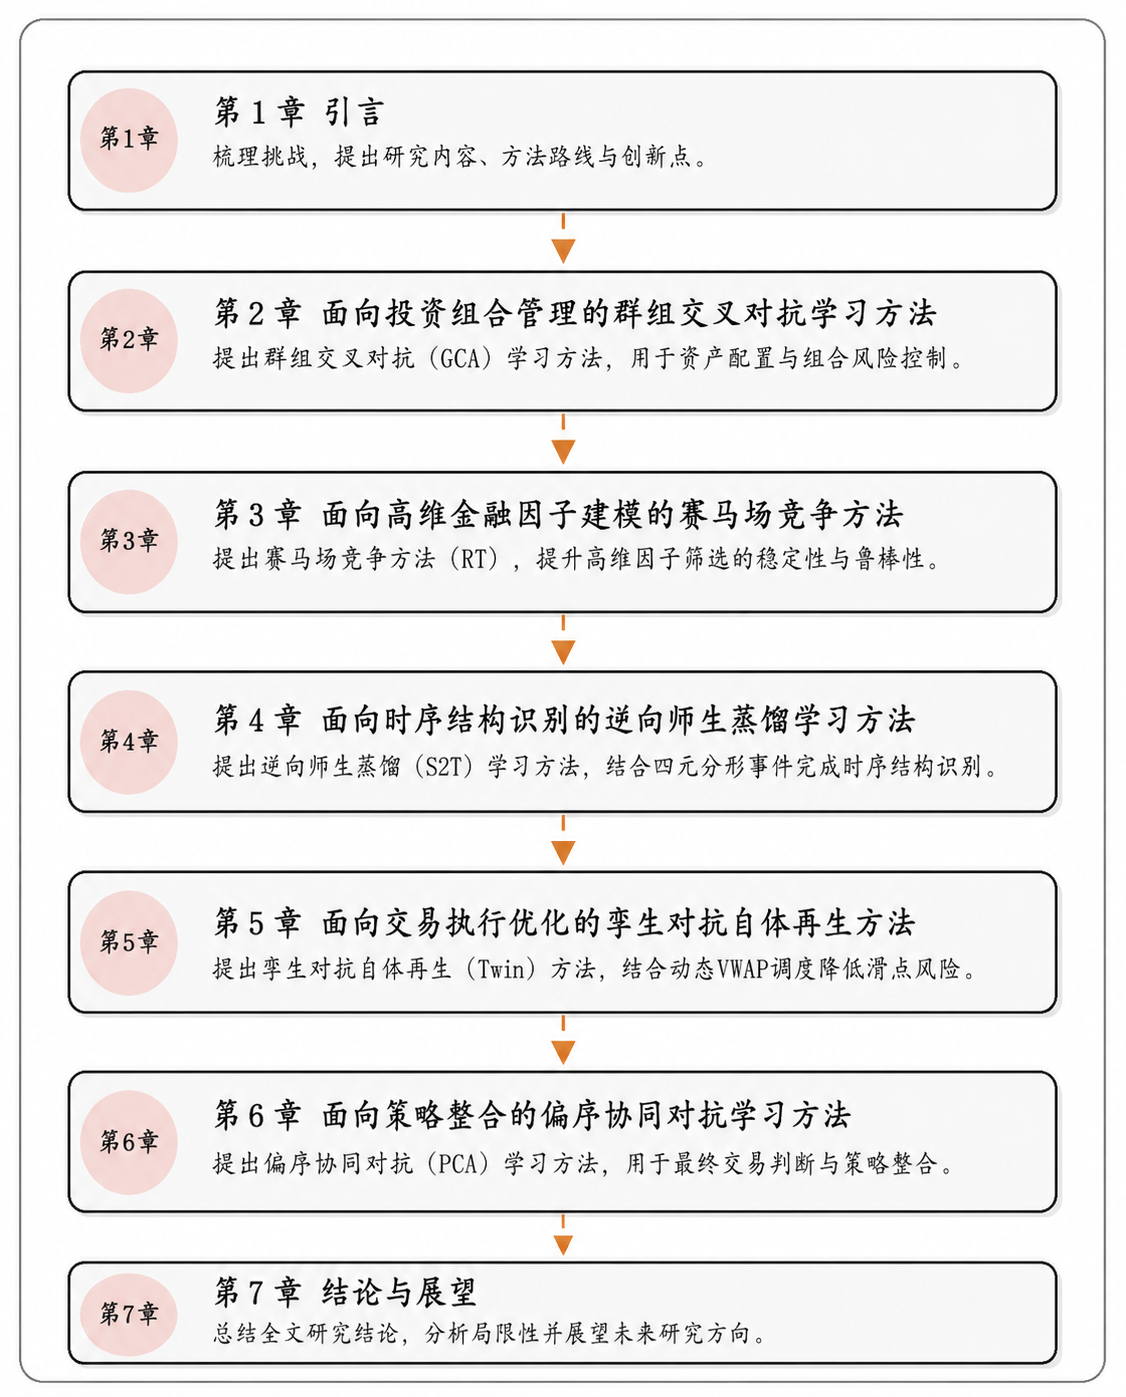
\includegraphics[width=0.95\textwidth]{figures/p1-3.png}
    \caption{本文章节结构与研究内容安排示意图}
    \label{fig:1-3}
\end{figure}

各章内容安排如下：

第1章引言。本章从对冲基金交易的系统性、自动化和博弈性特征出发，说明本文不将交易算法理解为单一价格预测模型，而是将其置于完整交易决策链条中加以讨论。在此基础上，本章梳理投资组合管理、高维金融因子建模、时序结构识别、交易执行优化和策略整合相关工作的研究现状，进一步明确本文的研究内容、方法路线和创新点。

第2章“面向投资组合管理的群组交叉对抗学习方法”。本章面向交易决策链中的资产选择与资金配置环节，重点讨论如何在多个资产之间识别配置对象并形成稳定资金配置。针对单一模型难以稳定刻画多资产相对关系、组合权重容易受噪声扰动以及风险约束难以嵌入配置过程等问题，本章提出群组交叉对抗（GCA）学习方法，通过多智能体群组之间的交叉校验与竞争约束，提高多资产配置中的信号稳定性和组合权重生成能力。

第3章“面向高维金融因子建模的赛马场竞争方法”。本章面向交易决策链中的因子依据形成环节，重点讨论哪些因子能够稳定支撑资产选择。在第2章关注多资产配置关系的基础上，本章进一步讨论高维因子空间中有效信息容易被噪声掩盖、模型容易在局部因子结构上过早收敛的问题。为此，本章提出赛马场竞争方法，通过动态选优、模型替换和成熟—新生模型之间的双向知识迁移，提升高维金融因子表征的稳定性和可解释性。

第4章“面向时序结构识别的逆向师生蒸馏学习方法”。本章面向交易决策链中的时机识别环节，重点讨论当前趋势结构是否具备交易意义。针对金融时间序列中局部噪声、伪结构和结构边界漂移导致交易时机判断不稳定的问题，本章以四元分形事件标注方法完成波浪结构量化表达，并设计逆向师生蒸馏机制，将弱模型中的失败经验反馈给强模型，从而抑制噪声过拟合并提升时序结构识别的稳定性。

第5章“面向交易执行优化的孪生对抗自体再生方法”。本章面向交易决策链中的订单执行环节，重点讨论如何降低滑点、市场冲击和执行偏差，并提升执行路径稳定性。在前序章节形成资产选择、因子依据和结构信号之后，交易信号还需要转化为可执行的订单路径。针对成交量预测误差、流动性错配和局部对抗失衡可能导致理论收益被执行成本侵蚀的问题，本章提出孪生对抗自体再生方法，通过复制—配对—分化和跨组修复机制，构建“预测成交量—执行路径—滑点控制—崩溃修复”的执行优化闭环。

第6章“面向策略整合的偏序协同对抗学习方法”。本章讨论交易决策链末端的最终交易判断形成问题。涨、跌、平等方向输出在这里不再被解释为孤立分类标签，而是对应买入、卖出或持有等交易动作。在问题定义、模型解释和评价口径上，本章承接资产配置、因子依据、结构信号和执行约束，提出偏序协同对抗（PCA）学习方法，用于改善最终判断中的边界稳定性、策略组织能力和跨资产泛化能力。

第7章结论与展望。本章对全文研究成果进行归纳，总结各章方法在交易决策链中的作用与创新点。随后分析当前研究仍存在的局限，并对后续研究方向进行展望。

本文第2章至第6章分别对应对冲基金交易决策链中的五个关键环节。第2章解决多资产配置对象选择与资金配置问题；第3章进一步解释因子依据形成，为资产选择提供稳定因子依据；第4章围绕时序结构识别，为交易时机判断提供方法支撑；第5章围绕交易执行路径优化，将前序交易信号转化为受滑点和市场冲击约束的订单执行路径；第6章则将方向分类结果组织为买入、卖出或持有等最终交易判断，并以偏序协同对抗学习方法完成策略整合。由此，全文形成“资产选择与资金配置—因子依据形成—时序结构识别—订单执行优化—最终交易判断”的递进关系。通过这种安排，本文既避免将五项研究写成互不相干的独立实验，也避免把所有机制压缩为单一总框架，而是在交易流程中为每一章确定相对明确的任务边界和方法作用。

     \chapter{面向投资组合管理的群组交叉对抗学习方法}

\section{问题的提出}

本章面向对冲基金交易决策流程中的投资组合管理环节，重点讨论多资产配置对象选择与资金权重生成问题。这里的资产选择并不是对单一资产涨跌方向的简单判断，而是指在多资产池中识别相对更具配置价值的标的，并进一步形成满足风险约束的组合权重。因此，本章所讨论的投资组合管理任务不是孤立的收益预测场景，而是多资产、多信号与多约束共同作用下的资金配置问题。围绕该场景，本章以群组交叉对抗（GCA）为核心，构建面向投资组合管理的多智能体对抗学习方法。GCA用于组织异构智能体进行多对多博弈，并在多资产之间比较相对强弱、控制组合风险敞口，将预测信号转化为更稳定的组合权重。需要强调的是，本章的研究边界落在投资组合管理本身，即回答“在多个资产之间如何形成更稳健的配置关系”这一问题；后续章节涉及的因子解释、结构识别、执行优化和策略整合，仅作为全文逻辑链条中的后续环节在本章中作必要衔接。

\subsection{传统投资组合管理方法的局限性}
% ===== 第一段：研究背景与现实意义 =====
金融时间序列预测是量化投资领域的核心挑战之一，其目标是从历史价格、成交量及其他市场数据中挖掘有效信息，以指导资产配置决策。早期金融预测研究主要依赖自回归、移动平均等统计时间序列模型，这类方法为金融时序的均值动态刻画提供了基础工具\cite{box2015time}。但是，对投资组合管理而言，仅说明收益均值的变化还不够，因为组合配置同时受到波动、相关性和风险暴露的共同约束。

在风险建模层面，单纯刻画条件均值并不足以解释金融市场中普遍存在的波动聚集现象。条件异方差框架将条件异方差引入金融序列分析，为收益波动与风险度量提供了重要方法基础\cite{engle2001garch}。这一类研究提醒本文，投资组合管理中的预测结果不能只看方向是否正确，还必须判断该预测所对应的风险暴露是否可被组合层面承受。

广义自回归条件异方差模型进一步扩展了波动率动态刻画能力，成为金融市场风险管理中的经典工具\cite{bollerslev1986generalized}。因此，资产收益预测必须同时面对“收益是否可预测”和“预测结果是否具有风险可承受性”两个问题。对于本章而言，这也意味着模型输出需要进一步转化为满足风险约束的组合权重，而不能停留在单一收益序列的拟合层面。

从组合配置角度看，预测模型的意义并不止于降低数值误差，而在于为资产配置提供可执行的风险收益判断。现代投资组合理论强调在收益与风险之间进行权衡，奠定了均值—方差框架的基础\cite{markowitz1952portfolio}。这一理论基础说明，组合管理的核心并不是挑出某一个预测收益最高的资产，而是在多个资产之间权衡收益、风险和相关性。

在此之后，资本资产定价模型从系统性风险定价角度解释了资产收益与风险暴露之间的关系\cite{sharpe1964capital}。这使得投资组合问题进一步从“预测收益”转向“识别收益背后的风险来源”。对于对冲基金交易而言，如果模型只输出单资产预测值，而不能区分该收益来自可承担的风险补偿还是不可控的系统性暴露，预测结果仍然难以直接用于配置。
进一步地，Black--Litterman 模型将市场均衡收益与投资者观点结合，为多资产配置中的先验约束与风险控制提供了常用框架\cite{black1992global}。由此可见，第二章并不是单纯追求价格序列预测精度，而是需要把预测信号放入组合权重、风险敞口和资金配置稳定性之中加以考察。

这些经典理论共同说明，面向对冲基金的预测模型不能只围绕单个价格序列展开，还需要服务于组合权重分配、风险敞口控制与长期收益稳定性。在真实交易环境中，预测结果只有经过资产比较、仓位控制与组合风险约束，才能最终转化为投资绩效。因此，本章讨论的核心问题是投资组合管理中的资产配置：模型不仅要预测单个资产的局部走势，还要比较不同资产之间的相对价值，并形成可执行的多资产权重分配方案。

随着机器学习方法的发展，支持向量机等非线性模型被用于金融时间序列预测，显示出相较传统线性模型的表达优势\cite{tay2001application}。这类模型的重要意义在于突破线性假设，为捕捉价格与成交量等变量之间的非线性关系提供了可能。但从投资组合管理角度看，非线性预测本身仍然只是配置决策的输入环节。

随后，长短期记忆网络通过门控记忆扩展金融时序建模能力\cite{hochreiter1997long}。这表明模型开始从静态特征拟合转向序列依赖建模，但其输出若不能被进一步比较和约束，仍可能停留在单资产预测层面。
门控循环单元在保持序列表达能力的同时简化结构\cite{cho2014learning}。这种结构简化有助于提升训练效率，但也提示本文需要在模型复杂度、收益预测稳定性和组合可执行性之间保持平衡。

自注意力序列模型则进一步强化长程依赖刻画\cite{vaswani2017attention}。这些模型分别代表了从非线性分类、循环记忆到全局依赖建模的技术演进，为处理金融序列中的复杂依赖关系提供了基础。与此同时，本章关注的重点并不是单纯选择更强的序列模型，而是如何把不同模型的预测结果组织成可交叉校验的多资产配置依据。

在金融应用中，长短期记忆网络已被用于股票市场方向预测，并在部分样本外区间表现出优于传统模型的效果\cite{fischer2018deep}。这说明深度序列模型能够提升方向预测能力，但方向预测并不等同于投资组合管理。组合管理还需要回答哪些资产更值得配置、配置多少以及在何种风险条件下配置。
针对长序列预测问题，Informer通过稀疏注意力机制提高建模效率\cite{zhou2021informer}。长序列建模能力的提升有助于扩展历史信息窗口，但在金融市场中，较长的信息窗口也可能引入过时状态和噪声，因此仍需要与市场状态筛选和组合约束结合。

Autoformer则利用分解结构与自相关机制强化长期依赖刻画\cite{wu2021autoformer}。这些研究扩展了模型处理时间依赖的能力，但组合管理关心的并不只是时序拟合本身。若模型只能改善单资产预测误差，而不能稳定比较多资产相对收益并生成可约束的组合权重，其优势仍难以转化为组合层面的风险收益表现。

在资产配置层面，投资组合自注意力序列模型等方法直接面向组合权重与风险调整收益进行建模，说明注意力机制已开始从预测环节延伸到投资组合决策环节\cite{kisiel2022portfolio}。这一变化表明，金融模型的目标不应局限于提高预测精度，还需要使输出能够对应资金配置和风险调整收益。
与此同时，深度强化学习投资组合管理研究表明，端到端地学习资产权重配置具有一定可行性\cite{jiang2017deep}。这类方法把投资组合作为序贯决策问题处理，使模型输出能够直接对应资产权重或交易动作。但在本章语境中，端到端并不意味着可以忽略模型之间的交叉校验，因为多资产配置中的错误预测会通过权重放大并转化为组合风险。

从本章的问题看，上述研究提供的启示并不是“用更复杂的模型替代传统模型”这么简单，而是说明投资组合管理需要把收益预测、权重生成和风险约束同时纳入建模过程。在鲁棒性方面，对抗深度强化学习投资组合方法表明，对抗训练可以服务于组合管理中的稳健决策\cite{liang2018adversarial}。这提示本文，投资组合管理中的对抗机制应当面向市场扰动和模型偏差，而不是仅作为生成模型形式上的装饰。

强化学习也被用于引入增强的资产运动状态，以改善投资组合管理中的状态表达与动作选择\cite{ye2020reinforcement}。因此，本章进一步关注如何通过多智能体之间的交叉评估，将单一模型输出转化为更稳健的多资产配置依据。
然而，将上述技术直接应用于金融预测时，仍会面临一系列独特挑战。首先，金融数据具有极低的信噪比，历史价格中的有效信息含量有限，大量波动来自随机交易行为与外生冲击\cite{lo2017economics}。这意味着即使模型在训练样本中捕捉到局部规律，也不能直接判断该规律具有稳定的交易价值。
同时，股票收益的随机游走假说长期受到实证检验，收益可预测性本身具有样本依赖与周期依赖特征\cite{lo1988stock}。因此，本章更强调多模型之间的交叉评估和组合层面的风险约束，避免将短期样本中的偶然预测优势直接放大为资产配置决策。
其次，金融市场具有显著的非平稳性，宏观冲击、流动性变化与参与者行为变化都可能导致训练样本与未来样本之间出现分布差异。以 2020 年新冠疫情期间的跨市场冲击为例，市场避险关系和资产间联动结构均可能出现阶段性变化\cite{conlon2020time}。因此，传统的均方误差损失难以有效反映投资组合的风险调整后收益特性，也难以保证模型在分布漂移环境下保持稳定。

\subsection{金融场景下多智能体博弈建模的挑战}
投资组合交易之所以需要多智能体建模，是因为其研究对象并不是单一资产的价格方向，而是多个资产之间相对收益、风险暴露、资金权重和市场状态共同作用下的动态配置过程。不同资产之间存在相关性变化、流动性差异和风险传导关系，单一模型即使能够在局部样本上取得较低预测误差，也未必能够稳定处理截面比较、仓位分配和组合层面的回撤控制。多智能体建模的意义在于，将不同资产视角、不同模型归纳偏置和不同风险约束组织为可交互的学习主体，使系统能够通过竞争、校验和协同约束刻画多资产配置中的动态博弈关系。

在这一背景下，多资产信号的不稳定性、不同品种之间的权重偏差以及风险暴露的阶段性变化，构成本章多智能体建模首先需要面对的问题。若模型仅对单一资产或单一生成器进行优化，则容易在市场状态切换时放大局部预测误差，进而影响组合层面的资金分配和回撤控制。因此，本节从多资产配置需求出发，讨论生成器、判别器与异构模型群之间如何形成可交叉评估、可动态校验的博弈结构。

生成对抗网络通过生成器与判别器之间的对抗博弈学习数据分布，已在图像生成、自然语言处理等领域得到广泛应用\cite{goodfellow2014generative}。对于本章而言，生成对抗思想的价值不在于生成一个孤立的价格序列，而在于利用判别器反馈约束预测序列的分布特征，使模型输出更接近可用于配置决策的市场状态描述。

标准生成对抗网络在训练中容易出现不稳定、模式崩溃和收敛困难等问题\cite{gui2023review}。这一问题对金融任务尤其敏感，因为金融收益分布本身具有强噪声、厚尾和状态切换特征，训练不稳定会直接影响后续组合权重的可靠性。

围绕训练不稳定问题，Arjovsky等人提出瓦瑟斯坦生成对抗网络，用推土机距离替代Jensen--Shannon 散度以缓解梯度消失问题\cite{arjovsky2017wasserstein}。这一类改进主要改变对抗训练的距离度量，为稳定学习分布差异提供了基础，但它仍然没有回答多资产配置中不同生成器如何分工的问题。

在此基础上，判别器约束和训练正则化进一步从梯度反馈层面改善对抗学习的稳定性。Gulrajani等人引入梯度惩罚以满足Lipschitz约束\cite{gulrajani2017improved}。这一方法说明，判别器约束的平滑性会直接影响生成器获得的梯度信号；在本文语境中，这对应于预测输出能否获得稳定的分布校正反馈。Miyato等人进一步通过谱归一化约束判别器权重矩阵的谱范数\cite{miyato2018spectral}。这类结构层面的稳定化处理提示本文，多判别器结构不能只增加判别器数量，还必须保证不同判别器输出的反馈信号不会放大金融噪声。Brock等人在大规模生成对抗网络中引入正交正则化与大规模训练策略\cite{Brock:2018rok}。上述研究共同说明，对抗训练的稳定性不仅取决于生成器能力，也取决于判别器反馈、正则约束和训练过程之间的协同关系。对于投资组合管理任务而言，本文更关注的是如何把这种稳定反馈转化为多资产预测结果之间的相互校验，而不是单纯提高样本生成质量。

针对时序数据，Yoon等人提出的时间序列生成对抗网络将对抗训练与逐步监督信号结合，为序列生成建模提供了代表性框架\cite{10.5555/3454287.3454781}。但是，金融数据的强非平稳性和极端事件仍会削弱这类模型的稳定性。本文借鉴时序对抗建模的思想，并不是为了生成完整的“假市场序列”，而是为了约束给定输入条件下预测输出与真实市场状态之间的联合关系。

单一生成器-判别器结构在分布漂移条件下容易性能衰退，多生成器架构虽然能够扩大覆盖范围，但在极端行情下也可能同步退化并形成局部共识幻觉\cite{ghosh2017multi}。因此，在投资组合管理中，仅提高生成质量并不足够，还需要引入多模型交叉评估、异构信号约束与组合权重输出机制。将生成对抗网络用于投资组合管理的原因在于，判别器可以作为“统计检验器”，约束生成器输出的多资产预测序列在分布特性上接近真实市场数据，并使这些预测信号进一步服务于组合权重分配。

从时间序列生成角度看，循环条件生成对抗网络在真实值时间序列生成任务中的应用说明，对抗式生成模型能够在一定程度上保留时间依赖结构\cite{esteban2017real}。这类研究的启示在于，金融时序预测不应只关注单点误差，还需要关注预测序列是否保留了市场变化过程中的条件依赖关系。
时间序列生成对抗网络进一步将对抗损失与逐步监督信号结合，为时间序列生成建模提供了代表性框架\cite{yoon2019time}。这些研究说明，对抗约束可以补充传统均方误差损失的不足；但在本章的组合管理任务中，分布约束最终仍需要回到多资产相对收益、权重生成和风险调整收益这三个配置目标上。

然而，标准 生成对抗网络 框架采用“一对一”（one-to-one）的生成器-判别器配对架构，在金融预测场景中面临四重主要挑战。
第一，模式崩塌（Mode Collapse）问题在金融时间序列中尤为突出。金融市场的收益率分布通常呈现尖峰厚尾、偏态等复杂特性，且在不同市场机制下表现出显著差异，早期关于投机价格变动的研究已经揭示了这类厚尾与非常态波动特征\cite{mandelbrot1963variation}。单一生成器在对抗训练中容易陷入“安全模式”，仅学习数据分布的少数主导模式，而忽视尾部风险和极端行情。
这一问题在多资产投资组合预测中更为严重：生成器可能只学会预测少数高流动性品种，而对低流动性品种产生系统性偏差。多智能体多生成器 生成对抗网络 的研究表明，通过多个生成器之间的竞争可以提升数据模式覆盖能力\cite{ghosh2017multi}。这提示仅依赖单生成器结构难以满足多资产配置对信号覆盖、权重分散和风险约束的要求，需要通过多模型交叉评估提高复杂金融数据分布的覆盖能力。

第二，“一对一”博弈拓扑限制了模型的多样性表达。理论上，多个具有不同归纳偏置的生成器可以分别专注于学习数据分布的不同方面，例如 门控循环单元更适合短期均值回归特征，自注意力序列模型更适合长期结构依赖。但在标准 生成对抗网络 框架下，不同生成器之间缺乏有效的竞争与协作机制，容易趋同于相似的预测输出。
围绕对抗训练稳定性，瓦瑟斯坦生成对抗网络从距离度量角度缓解了标准生成对抗网络训练不稳定问题，但其重点仍在单生成器分布逼近\cite{arjovsky2017wasserstein}。这类方法解决的是“如何让单个对抗系统更稳定”的问题，而不是“如何让多个预测模型在组合管理中形成互补分工”的问题。
谱归一化则通过约束判别器 Lipschitz 常数提高对抗训练稳定性，为复杂对抗系统提供了基础稳定化手段\cite{miyato2018spectral}。这些方法能够改善训练过程，但并未直接解决多个生成器之间如何分工的问题。
围绕多模型协同，相关研究已经从生成器组合、判别器协同和分布区域分工等角度对传统对抗结构进行了扩展。混合生成对抗网络通过多个生成器的概率组合来扩大生成分布的覆盖范围，为多生成器协同提供了参考\cite{hoang2018mgan}。对本文而言，这一思路的启示并不在于简单增加生成器数量，而在于说明不同生成器可以承担不同市场状态或资产关系下的预测职责，从而避免所有模型收敛到同一种输出模式。进一步看，生成器之间的差异只有在判别反馈能够形成多视角约束时，才可能真正转化为组合管理中的交叉校验能力。生成式多对抗网络讨论了多个判别器参与训练时的稳定性问题\cite{durugkar2017generative}。这一方向提示，判别器不应只作为单一真假判断器，而可以分别从不同角度检查生成器输出是否具有合理性。专业化判别器方法则表明，多判别器结构能够让不同判别器分别关注真实分布的不同子区域\cite{choi2022mclgan}。因此，多模型对抗结构的价值并不只是提升模式覆盖范围，更在于为本文后续构建“多生成器—多判别器”的交叉校验关系提供方法依据；但在投资组合管理任务中，模型输出最终还要服务于动态权重配置，因此仍需进一步结合金融市场的非平稳特征进行约束设计。

第三，静态优化范式与金融市场非平稳性之间存在矛盾。传统生成对抗网络在训练完成后，生成器和判别器的参数通常固定不变，而金融市场却具有显著的状态依赖性。大规模市场波动研究表明，市场波动在不同时间阶段会呈现聚集与结构变化特征\cite{plerou2002quantifying}。这意味着，投资组合管理模型面对的并不是稳定不变的数据分布，而是会随市场冲击、流动性变化和资产联动关系调整而持续变化的动态环境。对于多资产组合而言，分布漂移不仅会改变单个资产的收益预测误差，还会改变资产之间的相关性、波动暴露和权重约束条件。自适应市场假说进一步指出，市场有效性与投资者行为会随环境变化而动态演化\cite{lo2004adaptive}。从本文研究对象看，这一观点说明模型不能只在历史样本上获得一次性最优解，还需要在后续市场状态变化中持续校验预测信号和组合权重是否仍然有效。马尔可夫转换模型也从状态切换角度刻画了非平稳经济时间序列，为理解金融市场体制转换提供了经典工具\cite{hamilton1989regime}。这些研究共同说明，固定权重模型在分布漂移场景下可能迅速失效，本章提出的多智能体群组交叉对抗结构需要具备动态校验与更新能力，使系统能够在非平稳环境中维持较稳定的组合权重输出。

第四，训练效率与知识传承存在不足。生成对抗网络的训练过程以极小—极大博弈为本质，梯度信号在判别器与生成器之间来回振荡，容易导致收敛缓慢且不稳定。相关研究从理论角度分析了生成对抗网络训练不稳定的来源与改进方向\cite{arjovsky2017towards}。这一问题在多生成器、多判别器结构中会被进一步放大，因为每个生成器都需要接受判别反馈，多个模型之间还需要维持差异性与协同性。两时间尺度更新规则为生成对抗网络稳定训练提供了另一类实证与理论依据\cite{heusel2017gans}。然而，这类稳定化策略主要面向训练过程本身；在投资组合管理场景下，系统还必须考虑新数据到达、模型性能衰退以及旧模型知识如何被新模型继承的问题。知识蒸馏通过教师模型向学生模型传递软标签信息，为模型压缩与知识迁移提供了经典范式\cite{hinton2015distilling}。这一思路说明，模型更新不一定只能依赖从头训练，也可以通过已有模型向新模型传递有效知识来降低重复训练成本。深度互学习进一步表明，多个模型可以在相互学习过程中共同提升，而不必固定单一教师模型\cite{zhang2018dml}。由此可见，投资组合管理需要超越传统单模型和一对一对抗结构，在生成器、判别器与异构模型群之间建立可交叉评估、可动态协同、可传承知识的建模关系。与后续章节分别讨论高维金融因子建模、时序结构识别、交易执行优化和策略整合不同，本章首先解决的是多智能体如何服务于资产配置对象选择和资金配置的问题。

基于上述分析，本章需要解决的关键问题可以凝练为：在多资产组合管理中，如何在低信噪比、非平稳和多资产联动关系不断变化的条件下，稳定识别不同资产之间的相对配置价值，并将预测信号转化为风险约束下的组合权重。针对这一问题，GCA并不是简单增加模型数量，而是通过多生成器、多判别器之间的群组交叉对抗，使不同智能体在异构视角下相互校验，从而缓解单一模型导致的信号趋同、权重偏差和风险暴露失衡。由此，2.1提出的问题将在2.3的问题建模中被形式化，并在2.4的GCA算法设计中得到对应回应。

\section{相关工作}

本节围绕投资组合管理任务所依赖的相关研究展开梳理，重点说明现有方法如何从静态组合优化、深度学习资产配置逐步走向多模型协同与对抗式学习。与单纯讨论生成模型不同，本节关注的是这些研究如何服务于资产配置对象选择和资金配置的组合管理问题。

首先，传统投资组合管理研究以收益—风险权衡为核心，强调在多个资产之间进行权重分配和风险暴露控制。随着市场状态不断变化，静态权重配置方法难以充分刻画多资产之间的动态相关关系，因此后续研究逐渐引入机器学习与深度学习方法，以提高资产收益预测、风险估计和仓位调整的自适应能力。深度强化学习投资组合管理进一步将资产配置表示为序贯决策问题，使模型能够直接输出资产权重或交易动作。与2.1中对方法背景的介绍不同，本节更关注这些研究在投资组合管理任务中的具体不足，即它们是否能够把多资产相对关系、模型间校验和组合权重输出组织为同一个闭环。

其次，多智能体学习为投资组合管理中的多模型协同提供了方法基础。从多智能体学习角度看，多智能体 actor-critic 方法说明，不同智能体之间的交互关系可以被显式纳入学习过程\cite{lowe2017multi}。在多资产配置场景中，不同智能体可以对应不同时间尺度、不同模型结构或不同资产视角，通过协同与竞争共同形成组合决策。与单一模型相比，多智能体结构有助于降低某一模型对特定市场状态的过度依赖。

此外，对抗式学习为投资组合管理中的稳健性提供了重要启发。从鲁棒学习角度看，鲁棒对抗强化学习表明，在训练阶段引入对手或扰动有助于提升策略在不确定环境中的稳健性\cite{pinto2017robust}。这一思想与金融市场中的多主体竞争、策略交互和环境非平稳特征具有一致性。对于投资组合管理而言，对抗式训练的意义不只是生成更逼真的时间序列，而是通过判别反馈约束预测分布，使模型输出更适合后续资产权重配置。

最后，生成对抗学习和多模型协同研究为金融序列的分布约束与模型集成提供了重要工具。但在投资组合管理任务中，关键问题并不只是生成更逼真的时间序列，而是如何让多个异构模型在统一评价尺度下相互校验，并将其输出稳定转化为组合权重。因此，相关工作的不足主要体现在“多资产信号—模型交叉评估—组合配置输出”之间尚未形成闭环。

上述研究表明，投资组合管理已经从静态组合优化扩展到深度学习和强化学习驱动的动态资产配置；但在多资产信号稳定性、单模型配置偏差和模型间交叉校验方面仍存在不足。对于对冲基金交易而言，这些不足最终会影响资产配置对象识别与资金权重分配的稳定性：若模型只能给出单资产预测结果，而缺乏对多资产相对关系、组合权重和风险暴露的联合约束，预测优势就难以稳定转化为组合收益。基于此，本章提出面向投资组合管理的群组交叉对抗学习方法，将多个异构生成器和判别器组织为交叉博弈结构，以约束多资产配置过程中的信号稳定性、权重生成和组合风险。


\section{任务描述}

本节在相关工作基础上进一步明确本章的任务对象，并将2.1中提出的多资产配置问题转化为可建模的优化任务。投资组合管理并不等同于单资产方向预测，而是需要将多资产收益预测结果转化为组合权重，并在资金中性、风险调整收益与分布一致性等约束下形成可执行的配置决策。由此，本节先定义投资组合预测问题，再说明多资产收益预测与权重生成方式，最后给出本章方法需要满足的优化目标。这样处理的目的，是把资产配置任务具体落实为多资产相对收益比较、组合权重生成和风险调整收益优化三个环节，为后续GCA方法设计提供明确的任务边界。

\subsection{投资组合预测问题建模}

给定历史市场数据序列 $X = \{x_1, x_2, \ldots, x_T\}$，其中每个时刻的特征向量 $x_t$ 包含该资产的开盘价、最高价、最低价、收盘价与成交量及相关技术指标（如 指数平滑异同移动平均线、相对强弱指数、随机指标、真实波幅、布林带等）。模型的目标是基于历史窗口 $W$ 预测未来 $H$ 步的收益率序列：
\[
\hat{r}_{t+1:t+H} = f(x_{t-W+1:t}; \theta)
\]
其中 $\theta$ 为模型参数，$f(\cdot)$ 为预测函数。

需要说明的是，本章中的预测目标并不是单一时点的类别标签，而是给定历史市场窗口后的未来收益序列。为便于后续方法表述，本文将历史窗口 $x_{t-W+1:t}$ 视为条件输入，将真实未来收益序列记为 $r_{t+1:t+H}$，将模型输出记为 $\hat{r}_{t+1:t+H}$。因此，后文若使用 $y$ 表示监督目标，其含义对应真实未来收益序列，而非判别器训练中的二分类标签；判别器所使用的标签 $1/0$ 仅用于区分真实条件样本对与模型预测样本对。通过这一约定，可以避免将收益预测目标与对抗训练标签混同。


\subsection{多资产收益预测与组合权重生成}

在多资产投资组合场景下，设投资组合包含 $K$ 个资产，模型需同时预测 $K$ 个资产的未来收益率向量 $\hat{r}_t \in \mathbb{R}^K$。进一步，通过策略函数 $\phi(\cdot)$ 将预测收益率转化为资产权重 $w_t \in \mathbb{R}^K$，满足资金中性约束 $\sum_{i=1}^K w_{t,i} = 0$。具体采用连续多空策略：
\[
w_{t,i} = \frac{\hat{r}_{t,i} - \bar{r}_t}{\sum_{j=1}^K |\hat{r}_{t,j} - \bar{r}_t|}
\]
其中 $\bar{r}_t = \frac{1}{K}\sum_{j=1}^K \hat{r}_{t,j}$ 为截面均值。该策略专注于捕捉资产间的相对强弱关系（阿尔法），而非市场的系统性风险（贝塔）。


\subsection{组合风险约束与优化目标}

优化目标为最大化风险调整后收益，同时满足预测保真度和分布一致性约束：
\[
\max_{\theta} \mathcal{L}_{SR}(\theta) - \lambda_1 \mathcal{L}_{均方误差}(\theta) - \lambda_2 \mathcal{L}_{生成对抗网络}(\theta)
\]
其中 $\mathcal{L}_{SR}$ 为夏普比率损失（风险调整收益），$\mathcal{L}_{MSE}$ 为均方误差损失（数值保真度），$\mathcal{L}_{GAN}$ 为对抗损失（分布一致性）。从任务含义看，均方误差项用于保证资产收益预测的基本可用性，对抗损失用于约束预测序列与真实市场分布的一致性，夏普比率目标则将模型输出与投资组合的风险调整收益直接连接。三者共同对应本章问题中的信号稳定性、权重生成合理性和风险约束要求。



\section{群组交叉对抗方法}

本节围绕GCA展开方法设计。前一节已经给出投资组合预测、权重生成与优化目标，本节重点说明GCA如何通过异构生成器、判别器与组间交叉评估机制服务于多资产配置任务。具体而言，异构生成器用于从不同时间尺度和模型归纳偏置中提取多资产收益信号，多判别器用于从分布一致性角度检验生成结果，组间交叉对抗则用于避免单一模型在特定资产或特定市场状态上形成过度依赖。由此，GCA对2.1提出的三个问题形成直接回应：以多模型交叉评估提升信号稳定性，以多生成器竞争降低权重偏差，以风险调整目标约束组合输出。其他知识传递或状态修复机制只作为后续章节展开的辅助接口，不作为本章的主体方法。

需要说明的是，本文中的“生成器”并非传统生成对抗网络中从随机噪声直接生成样本的网络，而是在给定历史市场窗口和多资产状态特征条件下，输出未来收益预测或组合配置依据的条件预测模型。将其称为生成器，是因为该模型输出并不只接受点对点预测误差约束，还需要进入判别器构成的对抗训练过程，在数值保真度、条件分布一致性和组合风险调整目标之间同时接受约束。换言之，本章关注的并不是生成逼真的无条件金融样本，而是生成能够服务于投资组合权重配置的稳健预测输出。

%本节回顾与本章研究密切相关的三个领域的研究进展：多生成器生成对抗网络、知识蒸馏与模型压缩以及金融时间序列预测中的深度学习方法。通过对现有文献的系统梳理，明确当前研究的主要进展与不足，为本章的研究动机提供理论依据。

%\subsection{多生成器生成对抗网络}

% \subsubsection{问题域与方法发展}

%生成对抗网络（Generative Adversarial Network, GAN）自Goodfellow等人 \cite{goodfellow2014generative}提出以来，已成为生成建模领域的重要框架之一。GAN通过构建生成器与判别器之间的min-max对抗博弈，使生成器学习逼近真实数据分布。然而，标准GAN的训练过程存在显著的不稳定性问题，模式崩塌（mode collapse）是其中最为突出的核心问题，即生成器只学习到数据分布中的少数模式，而无法完整覆盖真实分布的多样性 \cite{arjovsky2017wasserstein}、\cite{mescheder2018training}。

%针对模式崩塌问题，相关研究者从不同角度提出一系列改进策略。Wasserstein GAN（WGAN） \cite{arjovsky2017wasserstein} 通过引入Wasserstein距离替代Jensen--Shannon 散度，实现了更稳定的训练过程。谱归一化 \cite{miyato2018spectral} 通过对判别器的权重矩阵进行谱归一化，约束判别器的Lipschitz常数，进一步提升训练稳定性。然而，这些方法主要关注单生成器场景下的训练稳定性，未能从根本上解决生成器多样性不足的问题。

% \subsubsection{多生成器架构的进展}

%多生成器架构作为缓解模式崩塌的另一重要研究方向，逐渐受到研究者的广泛关注。Ghosh等人 \cite{ghosh2017multi} 提出的MAD-GAN（Multi-Agent Diverse GAN）通过多个生成器共享一个判别器，要求判别器识别每个样本由哪个生成器产生，迫使其通过竞争学习不同的数据模式。Hoang等人 \cite{hoang2018mgan} 提出的MGAN（Mixture GAN）采用概率混合的方式组合多个生成器的输出，理论分析证明在均衡状态下，生成器混合分布与真实数据分布之间的Jensen-Shannon散度最小化，同时生成器之间的散度最大化，从而直接解决模式崩塌问题。Durugkar等人 \cite{durugkar2017generative} 进一步提出了多生成器多判别器架构（MGMD），通过引入多个判别器从不同角度评估生成样本。

%而MCL-GAN \cite{choi2022mclgan} 所提出的专业化判别器是多判别器架构的重要突破。该方法受多选择学习（Multiple Choice Learning）启发，让每个判别器专注于区分真实数据的一个子集，同时允许生成器自动找到潜在空间与真实数据空间之间的对应关系。这种设计在一定程度上缓解了模式崩溃问题，并通过共享骨干网络将计算成本控制在可接受范围内。然而，该方法的协作机制仅限于特征共享层面，未能建立生成器与判别器之间的深层对抗-协作关系。

% \subsubsection{金融应用与现有不足}

%在金融时间序列领域，研究者也将多生成器架构引入到序列生成任务中。Yoon等人 \cite{yoon2019time} 提出的TimeGAN在保留对抗损失的基础上引入了逐步监督损失（stepwise supervised loss），使模型更好地学习时序条件分布，该工作发表于NeurIPS 2019。Zhou等人 \cite{zhou2020mdgan} 提出的MDGAN采用多判别器结构增强对时序模式的评估能力。FinGAN \cite{wiese2020leveraging} 将多生成器架构应用于金融波动率建模，在衍生品定价任务上取得了显著提升。

%尽管现有多生成器GAN相关研究已取得了显著进展，但在以下方面仍存在明显不足：第一，不同生成器之间缺乏深度的竞争-协作机制，容易出现"伪多样性"——即生成器虽然架构不同，但预测输出高度相关，未能真正实现模式覆盖的扩展；第二，现有方法主要关注静态的模型集合，缺乏对数据分布时变性的自适应能力；第三，缺乏对生成器健康状态的监控机制，无法在模型性能衰退时自动触发修复。

%\subsection{知识蒸馏与模型压缩}

% \subsubsection{知识蒸馏的基本理论与单向模式}

%知识蒸馏（Knowledge Distillation）最初由Hinton等人 \cite{hinton2015distilling} 提出，旨在将大型教师模型（teacher model）的知识迁移到轻量级学生模型（student model），实现模型压缩的同时保持预测性能。其核心思想是让学生模型学习教师模型的"软标签"（soft labels），而非仅学习硬标签（hard labels），从而传递教师模型在类别关系上的暗含知识。

%传统知识蒸馏采用单向的知识传递模式，即教师模型参数固定，学生模型从教师输出中学习。这种模式在模型压缩场景中效果显著，但存在如下局限：其一，当学生模型能力接近教师模型时，蒸馏信号趋于消失，训练效率降低；其二，单向传递无法利用学生模型学习过程中的有价值信息，造成知识浪费；其三，教师模型本身的偏差会完整传递到学生模型，无法纠正。

% \subsubsection{双向知识流动与动态模型选择}

%为克服单向蒸馏的局限，研究者提出了多种双向知识流动机制。Zhang等人 \cite{zhang2018dml} 提出的深度互学习（Deep Mutual Learning, DML）让多个学生模型相互学习，每个模型既是教师也是学生，实现了知识的双向传递。Yuan等人 \cite{yuan2020revisiting} 提出的基于标签自蒸馏（Label Self-Distillation）方法，让模型从自身的历史输出中学习，实现知识的跨时态传递。Lee等人 \cite{lee2019self} 进一步提出了跨模型自蒸馏框架，通过模型自身的不同训练阶段实现知识精炼。

%在模型选择与动态组合领域，AutoML和神经架构搜索（Neural Architecture Search, NAS）技术 \cite{elsken2019neural} 提供了自动化模型选择的可能性。然而，这些方法通常需要大量的计算资源，且搜索空间的设计高度依赖人工经验，在金融时序预测场景下的系统性应用仍处于早期阶段。

% \subsubsection{蒸馏机制与对抗学习的结合空白}

%知识蒸馏与模型选择的研究进展为本章的逆向师生蒸馏（S2T）提供了理论基础。然而，现有方法未能将蒸馏机制与对抗学习有机结合，也缺乏在金融时序预测场景下的系统性验证。

%\subsection{面向金融时序预测的深度学习方法}

% \subsubsection{问题背景与传统方法的局限}

%金融时间序列预测是量化投资领域的核心问题。传统计量经济学方法，如自回归移动平均模型（AutoRegressive Moving Average, ARMA）和广义自回归条件异方差模型（Generalized AutoRegressive Conditional Heteroskedasticity, GARCH） \cite{bollerslev1986generalized}、\cite{engle2001arch}，在建模金融数据的条件均值和方差动态方面取得了重要进展。然而，这些线性模型难以捕捉数据中的非线性依赖关系和复杂交互模式。

% \subsubsection{深度学习方法的应用与挑战}

%深度学习技术的引入为金融时间序列建模带来了新的可能性。循环神经网络（Recurrent Neural Network, RNN）及其变体长短期记忆网络（Long Short-Term Memory, LSTM）和门控循环单元（Gated Recurrent Unit, GRU） \cite{hochreiter1997lstm}、\cite{cho2014learning} 能够有效捕捉时间序列中的长程依赖关系，在股价预测 \cite{fischer2018deep}、波动率建模 \cite{li2018deep} 等任务上展现出优于传统方法的性能。Transformer架构 \cite{vaswani2017attention} 通过自注意力机制建模任意位置之间的依赖关系，在自然语言处理取得巨大成功后，也被广泛应用于时间序列分析 \cite{zhou2021informer}、\cite{wu2020autoformer}。

%然而，将深度学习直接应用于金融预测面临独特的挑战。首先，金融数据具有极低的信噪比，历史价格中的有效信息含量极低，大部分为随机噪声 \cite{lo2017economics}。单纯的监督学习容易导致模型过度拟合历史噪声，在样本外表现急剧下降。其次，金融市场具有显著的非平稳性，如2020年新冠疫情、2022年全球通胀等事件易导致数据分布发生剧烈变化 \cite{conlon2020time}。基于历史数据训练的模型在这种"分布漂移"场景下性能衰退严重。第三，金融决策需要同时考虑收益与风险，传统的均方误差（Mean Squared Error, MSE）损失无法反映投资组合的风险调整后收益特性。

% \subsubsection{多角度的改进方案与多模型协同}

%为解决上述问题，研究者从多个角度进行了探索。在损失函数设计上，Kelly等人 \cite{kelly2019deep} 提出了面向金融决策的定制化损失函数，将夏普比率等风险指标纳入优化目标。Fang等人 \cite{fang2020deep} 进一步提出了面向多资产组合优化的对抗训练框架，通过判别器约束生成预测的统计特性。在模型集成方面，种种研究表明，多模型的动态组合能够有效提升预测的鲁棒性 \cite{caruana1997multitask}、\cite{dietterich2000ensemble}。然而，如何设计有效的多模型协同机制仍是开放性问题。

% \subsubsection{GAN在金融预测中的应用与不足}

%将GAN应用于金融预测是近年来的新兴研究方向。

%而生成对抗网络（GAN）凭借其独特的对抗学习特性，为该问题的解决提供了新的技术路径，也成为近年来金融预测领域的新兴研究方向。Esteban等人 \cite{esteban2017real} 提出的Real-valued GAN（RGAN）能够生成逼真的金融时间序列样本。SeqGAN \cite{yu2017seqgan} 将GAN扩展到离散序列生成任务，为金融信号生成提供了新思路。COTED提出了面向金融预测的条件时序对抗网络，在资产收益率预测任务上取得了显著进展。然而，这些方法主要关注单生成器-单判别器架构，未能充分利用多模型协同的潜力。

% \subsection{现有文献的空白与本章贡献}

%综合上述文献的梳理与分析可以发现，当前研究在以下三个方面仍存在系统性空白，这些空白也正是本章的核心研究动机：
%\begin{enumerate}
%\item \textbf{多生成器协同机制的设计不足}：现有方法虽然引入了多个生成器，但缺乏深度的竞争-协作机制来确保生成器之间的多样性。“伪多样性”问题导致集成收益被显著削弱。
%\item \textbf{单向知识传递的效率瓶颈}：传统蒸馏和互学习方法未能与对抗学习有机结合，知识传递的效率和效果受到限制。
%\item \textbf{缺乏模型健康监控与自体再生机制}：现有方法缺乏对模型自身状态的实时监控能力，无法在检测到性能衰退时自动触发修复。
%\end{enumerate}

%针对上述空白，本章提出多智能体群组交叉对抗学习框架（MGCA）。该框架通过三个创新点的系统性协同解决上述问题：群组交叉对抗（GCA）增加模型多样性、逆向师生蒸馏（Student-to-Teacher Distillation, S2T）实现双向知识流动、孪生对抗自体再生（Twin）提供异常监控与自体再生能力。
%现有研究尚缺乏一个系统性的框架来同时应对多样性、知识传递和监控这三个方面的挑战。单独的改进（如改进损失函数、引入多生成器或应用蒸馏机制）往往只能部分缓解问题，难以全面应对金融时间序列预测中多模型协同学习的复杂性。因此，设计一个有机整合多个创新点的完整框架，使其在金融预测任务中充分发挥协同效应，成为了一个迫切的研究需求。
\subsection{群组交叉对抗的建模动因与基本假设}

群组交叉对抗机制是多生成器-多判别器结构的核心组成部分，也是本章面向投资组合管理任务的主要方法。其设计目的不是简单增加模型数量，而是通过异构生成器与判别器之间的交叉对抗学习，建立一个能够服务多资产收益判断、组合权重生成和风险暴露约束的群组博弈结构，从而降低单一模型在复杂资产池中出现信号趋同、模式崩塌或配置偏差的风险。

在传统的生成对抗网络中，一对一的对抗训练容易导致生成器只学习到数据分布的某一小部分特征，形成模式崩塌。在投资组合管理场景中，这种问题会进一步表现为模型过度依赖少数高流动性资产或单一市场状态，从而造成组合权重分配偏差。为此，本章引入群组交叉对抗机制，让每个生成器都与多个判别器进行对抗，同时每个判别器也评估多个生成器的输出。这种交叉拓扑结构具备三重核心优势：其一，不同生成器可以从不同时间尺度和归纳偏置出发学习资产收益结构；其二，判别器的多元反馈能够约束预测分布，减少资产配置中的单模型偏差；其三，生成器与判别器在动态博弈中共同提升，使组合权重生成过程更加稳健。

进一步地，本文中的判别器也不是对单个收益率数值作真假判断，而是对“历史输入—未来输出”构成的条件样本对进行分布一致性检验。具体而言，真实样本对由历史市场窗口与真实未来收益序列构成，可表示为 $(x_{t-W+1:t}, r_{t+1:t+H})$；生成样本对则由同一历史市场窗口与生成器预测收益序列构成，可表示为 $(x_{t-W+1:t}, \hat{r}_{t+1:t+H})$。判别器的目标是在给定历史输入条件下，区分输出序列是否符合真实市场中的条件联合分布关系。因此，判别器提供的并不是传统意义上的“真假图片”反馈，而是对预测结果与市场条件之间匹配程度的分布约束。
%这种交叉拓扑结构使得：
%\begin{enumerate}
    %\item 多尺度特征学习：不同的生成器可以专注于学习数据分布的不同方面
    %\item 分布正则化：判别器的多元反馈防止生成器趋同
    %\item 协同进化：生成器与判别器在动态博弈中共同提升
%\end{enumerate}

基于上述设计，本章的群组交叉对抗方法建立在四个基本假设之上：第一，多资产收益结构具有异质性，不同资产和不同时间尺度下的有效信号并不完全一致；第二，不同生成器具有差异化归纳偏置，能够从短期波动、中期依赖和长期结构等角度形成互补表征；第三，判别器的交叉反馈能够对生成结果进行分布层面的外部校验，降低单一判别器偏好造成的配置偏差；第四，组合层输出必须接受风险调整收益、资金中性和辅助状态校验等约束，不能仅以预测误差最小化作为目标。由此，本小节重点说明群组交叉对抗的建模动因与基本假设。完整训练流程、可选增强机制与复杂度分析将在“多智能体群组交叉对抗方法”小节中集中说明，以避免理论假设与训练流程混杂。


%\subsection{数学范式描述}

% 下面构建群组交叉对抗框架的数学范式。设生成器集合 
% \[
% \mathcal{G} = \{ \{ G_{i,j} \}_{j=1}^{M} \}_{i=1}^{N}, 
% \] 
% 判别器集合 
% \[
% \mathcal{D} = \{ \{ D_{i,j} \}_{j=1}^{M} \}_{i=1}^{N},
% \] 
% 其中 $i$ 为组编号，$j$ 为组内成员编号。这里，$N$ 表示组的数量，$M$ 表示每组的生成器/判别器成员数量。该集合定义用于刻画 GCA 框架中层次化、多智能体的结构。

% \paragraph{1. 组间对抗损失 (Cross-Group Loss)}  
% 组间对抗是 GCA 的核心创新，它迫使组内生成器不仅需要骗过本组判别器，还要能够欺骗异构组的判别器，从而学习更通用、更鲁棒的特征。数学形式如下：
% \begin{equation}
% \mathcal{L}_{\text{cross}}^{(i,j)} =
% \sum_{k \neq i} \sum_{l=1}^{M} 
% \Big[ \mathbb{E}_{x \sim P_{data}} [\log(1 - D_{k,l}(G_{i,j}(x)))] 
% + \lambda_{recon} \| G_{i,j}(x) - x \|_2^2 \Big]
% \end{equation}

% 其中，第一项衡量生成器欺骗异组判别器的能力，即生成器输出的“对抗性”，迫使模型捕捉跨架构的高阶统计特征；第二项为重构损失，保证生成器输出在数值上尽量贴近真实数据，避免生成不可用或失真信号；$\lambda_{recon}$ 控制重构约束的强弱。
% %\end{itemize}
% %\begin{itemize}
%     %\item 第一项衡量生成器欺骗异组判别器的能力，即生成器输出的“对抗性”，迫使模型捕捉跨架构的高阶统计特征。
%     %\item 第二项为重构损失，保证生成器输出在数值上尽量贴近真实数据，避免生成不可用或失真信号。
%     %\item $\lambda_{recon}$ 控制重构约束的强弱。
% %\end{itemize}

% \paragraph{2. 组内蒸馏损失 (Intra-Group Distillation)}  
% 组内蒸馏通过精英成员向组内其他成员传递高阶知识，加快弱成员收敛并提升整体组表现：
% \begin{equation}
% \mathcal{L}_{\text{distill\_intra}}^{(i)} = 
% \lambda_{distill} \sum_{j \neq j^*} \| G_{i,j}(x) - \text{StopGrad}(G_i^*(x)) \|_2^2
% \end{equation}
% 其中，$G_i^*$ 是组内最优生成器（组冠军）；StopGrad 操作阻断梯度回传到教师模型，只更新学生模型，确保知识传递稳定；$\lambda_{distill}$ 控制蒸馏强度。这一过程类似“局部精英学习”，让每组快速形成内部共识，同时保留组间差异。
% %\end{itemize}
% %\begin{itemize}
%     %\item $G_i^*$ 是组内最优生成器（组冠军）。
%     %\item StopGrad 操作阻断梯度回传到教师模型，只更新学生模型，确保知识传递稳定。
%     %\item $\lambda_{distill}$ 控制蒸馏强度。
% %\end{itemize}


% \paragraph{3. 全局蒸馏损失 (Global Distillation)}  
% 全局蒸馏在组间引入知识传播，将全局最优模型的高阶特征共享给各组冠军：
% \begin{equation}
% \mathcal{L}_{\text{distill\_global}} = 
% \lambda_{distill} \sum_{i=1}^{N} \| G_i^*(x) - \text{StopGrad}(G^{**}(x)) \|_2^2
% \end{equation}
% 其中 $G^{**}$ 为全局最优生成器（总冠军）。这一机制保证局部优势能够快速提升至全局水平，实现跨组的知识融合。

% % \paragraph{4. MSE 损失 (数值保真度约束)}  
% % MSE 损失确保生成器输出在数值上贴近真实收益率序列：
% % \begin{equation}
% % \mathcal{L}_{MSE} = \frac{1}{T} \sum_{t=1}^{T} \| \hat{r}_t - r_t \|^2
% % \end{equation}
% % 它提供了强梯度信号，防止生成器陷入高阶统计特征对齐但整体偏离真实数值的情况。

% \paragraph{5. Sharpe 损失 (经济效用约束)}  
% Sharpe Loss 将投资组合的风险—收益特性引入模型训练，使生成器输出不仅在数值上合理，也在投资决策上稳健：
% \begin{equation}
% \mathcal{L}_{Sharpe} = - \lambda_{sr} \frac{\mathbb{E}[\hat{r}_p]}{\sqrt{\text{Var}(\hat{r}_p) + \epsilon}}
% \end{equation}
% 分子项奖励模型捕捉正收益机会，分母项惩罚高波动输出，实现风险厌恶行为。

% \paragraph{6. 最终生成器总损失}  
% 将以上所有约束整合，GCA 模块的总损失为：

% \begin{equation}
% \mathcal{L}_{Total} = 
% \lambda_{mse} \mathcal{L}_{MSE} 
% + \lambda_{gan} \Big( \mathcal{L}_{\text{cross}} + \mathcal{L}_{\text{distill\_intra}} + \mathcal{L}_{\text{distill\_global}} \Big) 
% + \lambda_{sharpe} \mathcal{L}_{Sharpe}
% \end{equation}

% \noindent
% 其中，
% %\begin{itemize}
%     %\item $\lambda_{gan}$ 控制对抗与蒸馏的综合影响；
%     %\item $\lambda_{mse}$ 保证生成器在数值上逼近真实收益率；
%     %\item $\lambda_{sharpe}$ 将经济学约束纳入训练；
%     %\item 该总损失框架可表述为 $\mathcal{L}_{Total} = \lambda_{mse}\mathcal{L}_{MSE} + \lambda_{gan}\mathcal{L}_{GAN} + \lambda_{sharpe}\mathcal{L}_{Sharpe}$ ，其中 $\mathcal{L}_{GAN}$ 对应于 GCA 的跨组/组内/全局蒸馏复合损失。
% %\end{itemize}
%  $\lambda_{gan}$ 控制对抗与蒸馏的综合影响； $\lambda_{mse}$ 保证生成器在数值上逼近真实收益率； $\lambda_{sharpe}$ 将经济学约束纳入训练； 该总损失框架可表述为 $\mathcal{L}_{Total} = \lambda_{mse}\mathcal{L}_{MSE} + \lambda_{gan}\mathcal{L}_{GAN} + \lambda_{sharpe}\mathcal{L}_{Sharpe}$ ，$\mathcal{L}_{GAN}$ 对应于 GCA 的跨组/组内/全局蒸馏复合损失。
% \end{itemize}

% \noindent
% 通过这种分层次、多目标统一的损失设计，多智能体群组交叉对抗框架能够在保持模型架构异质性与追求全局最优预测性能之间达到动态平衡。



% %\subsection{训练参数说明}
% \begin{table}[h]
% \centering
% \begin{tabular}{l l c}
% \hline
% \textbf{类别} & \textbf{参数名称} & \textbf{设定值} \\
% \hline
% 循环控制 & 宏观循环次数 ($N_{global}$) & 3 \\
%  & 组内循环次数 ($N_{inner}$) & 3 \\
%  & 组间循环次数 ($N_{outer}$) & 3 \\
% \hline
% 优化权重 & 蒸馏权重 ($\lambda_{distill}$) & 0.5 \\
%  & 重构权重 ($\lambda_{recon}$) & 1.0 \\
%  & GAN 总权重 ($\lambda_{gan}$) & 1.0 \\
%  & MSE 权重 ($\lambda_{mse}$) & 1.0 \\
%  & Sharpe 权重 ($\lambda_{sharpe}$) & 0.1 -- 0.5\\
% \hline
% 学习率 & 生成器学习率 & $2 \times 10^{-4}$ \\
%  & 判别器学习率 & $2 \times 10^{-4}$ \\
% \hline
% 其他 & 批量大小 & 32 \\
%  & 优化器 & Adam \\
%  & 正则化 & StopGrad \\
% \hline
% \end{tabular}
% \caption{GCA 模块核心训练参数配置}
% \end{table}




% %\subsection{异构生成器模块}

% 金融时间序列在统计特性上天然具有多视图结构：在短时间尺度内表现为高噪声、高波动过程，而在较长时间尺度上则逐渐显现趋势性与结构性特征。为系统刻画这一现象，MGCA 在生成器层面显式集成多种具有不同时间归纳偏置的深度神经网络结构，构成异构生成器集合。

% 具体而言，生成模块主要包括以下两类模型：
% \begin{enumerate}
%     \item \textbf{循环神经网络变体（GRU / LSTM）}：依托门控递归结构，这类模型能够有效捕捉序列的条件依赖关系与近似马尔可夫特性，尤其适用于刻画短期高频波动以及中期均值回归行为。
%     \item \textbf{Transformer 架构}：基于多头自注意力机制，Transformer 能够突破递归模型在长距离依赖建模上的固有局限，从而更有效地识别跨时间尺度的全局趋势与稀疏结构性关联。
% \end{enumerate}

% 为保证不同生成器在时间维度上的因果一致性与信息可比性，本章构建了多尺度输入窗口机制。具体设定窗口长度集合
% \[
% W \in \{5, 10, 20\},
% \]
% 分别对应周度、双周度与月度市场周期。该设计使模型能够在统一框架下同时学习微观结构噪声与宏观市场信号，并在对抗博弈过程中完成跨尺度信息的隐式融合。

% %\subsection{多智能体对抗博弈机制}

% 在多生成器并行建模的情形下，传统 GAN 框架往往容易出现模式崩塌，即生成结果趋向于少数“安全但信息贫乏”的模式。为缓解这一问题，MGCA 引入自适应元加权对抗机制，将对抗过程从静态博弈扩展为动态协同—竞争的演化过程。

% \paragraph{判别器优化目标}
% 对于判别器集合中的任意 $D_j$，其损失函数定义为加权对抗损失：
% \begin{equation}
%     \mathcal{L}_{\mathcal{D}} =
%     \sum_{j=1}^{N}
%     \left[
%         - \log D_j(X_j, Y_j)
%         - \sum_{i=1}^{N}
%         W_{ji}
%         \log \bigl(1 - D_j((X,Y)_{G_i \rightarrow D_j}) \bigr)
%     \right],
% \end{equation}
% 其中 $W \in \mathbb{R}^{N \times N}$ 为动态权重矩阵，用以刻画生成器 $G_i$ 对判别器 $D_j$ 的相对影响强度。该权重由元学习网络自适应更新，使判别器能够重点关注更具区分难度的生成模式。

% \paragraph{混合多目标优化范式}

% 为在高维、非平稳的金融时间序列环境中构建稳健的决策信号，MGCA 采用由多个互补目标组成的混合优化框架。生成器的总体损失函数定义为：
% \begin{equation}
%     \mathcal{L}_{Total}
%     =
%     \lambda_{mse} \mathcal{L}_{MSE}
%     +
%     \lambda_{gan} \mathcal{L}_{GAN}
%     +
%     \lambda_{sharpe} \mathcal{L}_{Sharpe}.
% \end{equation}

% 其中，各损失项分别从数值保真度、分布一致性与经济效用三个层面对生成过程进行约束，并通过自适应权重管理器在训练过程中动态平衡其相对重要性。该目标体系的每一项通过自适应权重管理器（Adaptive Weight Manager）动态平衡，具体物理含义如下：

% \paragraph{1. MSE Loss}
% 均方误差（MSE）构成了优化的基础锚点，约束模型预测的收益率曲线 $\hat{r}$ 在欧氏空间上尽可能贴近真实收益率 $r$：
% \begin{equation}
%     \mathcal{L}_{MSE} = \frac{1}{T} \sum_{t=1}^{T} \|\hat{r}_t - r_t\|^2
% \end{equation}
% 由于金融数据极高的信噪比，单纯的对抗训练容易导致模型迷失方向（Mode Collapse）。MSE 项通过提供强梯度的监督信号，确保了预测结果在数值上的基本准确性，防止模型生成虽然统计分布逼真但与当前市场状态脱节的“幻觉”信号。

% \paragraph{2. GAN Loss}
% 为了克服 MSE 对高频噪声过拟合的倾向，我们引入了群组交叉对抗机制。该机制通过最大化判别器的误判概率，迫使生成器学习收益率序列的高阶统计特征（如偏度与峰度）：
% \begin{equation}
%     \mathcal{L}_{GAN} = - \sum_{j=1}^{M} W_{ij} \cdot \log(D_j(G_i(z)))
% \end{equation}
% 其中 $W_{ij}$ 为自适应对抗权重，由系统根据判别难度动态调整。这不仅是一种有效的正则化手段，更使模型具备了跨时间尺度的分布对齐能力，有助于捕捉隐含的市场状态转移规律。

% \paragraph{3. 经济学效用引导 (Sharpe Ratio Loss)}
% 传统的深度学习预测往往仅关注均方误差（MSE）的最小化。然而在金融场景中，低 MSE 并不等同于高投资回报。为了弥合预测与决策的鸿沟，我们引入了可微的夏普比率损失作为顶层引导，通过引入夏普比率损失（Sharpe Ratio Loss, $\mathcal{L}_{SR}$），我们将投资组合理论中的“均值-方差优化”思想直接嵌入到神经网络的梯度流中：
% \begin{equation}
%     \mathcal{L}_{Sharpe} = - \lambda_{sr} \cdot \frac{\mathbb{E}[\hat{r}_p]}{\sqrt{\text{Var}(\hat{r}_p) + \epsilon}}
% \end{equation}


% 其中 $\hat{r}_p$ 为生成的投资组合预测收益率序列，$\epsilon$ 为防止除零的数值稳定项。

% 该损失函数具有双重调节作用：分子项激励模型捕捉正向收益机会，分母项则对高波动预测施加惩罚。这促使神经网络在追求高回报的同时兼顾稳定性，体现了“风险厌恶”的决策特征。且该损失函数具有以下关键的经济学属性：
% \begin{enumerate}
%     \item 收益激励：分子项 $\mathbb{E}[\hat{r}_p]$ 产生负梯度，直接推动模型在预测中寻找正向收益机会。
%     \item 内生风险控制：分母项 $\sqrt{\text{Var}(\hat{r}_p)}$ 对高波动预测施加惩罚。这意味着如果模型为了追求高收益而生成了极不稳定的预测轨迹，损失值反而会增加。
% \end{enumerate}


\subsection{群组交叉对抗架构与多智能体交互建模}

在完成投资组合预测目标、组合权重生成方式和优化约束定义后，本节转入GCA中的多智能体交互结构，重点说明异构生成器、判别器和群组拓扑如何共同构成服务于投资组合管理的交叉对抗机制。
将上述投资组合预测问题建模为多智能体博弈过程。设异构生成器集合 $\mathcal{G} = \{G_1, G_2, \ldots, G_N\}$，每个生成器 $G_i$ 对应一种神经网络架构（如门控循环单元、长短期记忆网络和自注意力序列模型），具有不同的归纳偏置：
\textbf{门控循环单元}擅长捕捉短期均值回归特性，适合高频微观结构；\textbf{长短期记忆网络}擅长建模中长程依赖，适合中期波段分析；
 \textbf{自注意力序列模型}擅长捕获全局趋势依赖，适合长期结构特征。

%\begin{itemize}
    %\item \textbf{GRU}：擅长捕捉短期均值回归特性，适合高频微观结构
    %\item \textbf{LSTM}：擅长建模中长程依赖，适合中期波段分析  
    %\item \textbf{Transformer}：擅长捕获全局趋势依赖，适合长期结构特征
%\end{itemize}

判别器集合 $\mathcal{D} = \{D_1, D_2, \ldots, D_M\}$ 用于评估生成器预测的真实性。与标准 生成对抗网络 的“一对一”配对不同，本框架采用全连接的多对多博弈拓扑结构，每个生成器需同时与多个判别器进行对抗训练。

进一步将生成器和判别器组织为层次化群组结构：
\[
\mathcal{G} = \{ \{ G_{i,j} \}_{j=1}^{M} \}_{i=1}^{N}, \quad
\mathcal{D} = \{ \{ D_{i,j} \}_{j=1}^{M} \}_{i=1}^{N}
\]
其中 $i$ 为组编号，$j$ 为组内成员编号。生成器 $G_{i,j}$ 需要欺骗异组判别器 $D_{k,l}$ ($k \neq i$)，学习跨架构的通用特征；判别器则需区分真实数据分布与生成器输出分布。

%\subsection{多生成器多判别器平衡问题建模}

在投资组合管理任务中，多生成器-多判别器架构需要处理的不是抽象的模型数量增加问题，而是三个直接关系到组合配置质量的平衡问题：

\paragraph{1.多样性-稳定性平衡} 多个生成器需保持输出多样性，以覆盖不同资产和不同市场状态下的收益结构；同时，组合权重又不能因模型差异而频繁跳变。因此，多样性约束服务于资产覆盖范围，稳定性约束服务于权重生成的可执行性。定义多样性损失 $\mathcal{L}_{div}$ 衡量生成器输出间的差异性，稳定性损失 $\mathcal{L}_{stab}$ 衡量训练过程的梯度平滑度：
\[
\mathcal{L}_{balance} = \alpha \mathcal{L}_{div} - \beta \mathcal{L}_{stab}
\]

\paragraph{2.竞争-协作平衡} 生成器之间既存在竞争，即不同结构模型需要在判别反馈中证明自身输出更接近真实市场分布；也存在协作，即系统需要综合不同模型对多资产相对收益的判断，而不是让单一模型完全支配组合配置。定义竞争强度 $\eta_{comp}$ 和协作强度 $\eta_{coop}$，通过元学习权重网络自适应调节：
\[
w_{i,j}^{(t)} = \text{MetaWeightNet}(X_t, \{\hat{r}_t^{(i)}\}; \phi)
\]

\paragraph{3.探索-利用平衡} 生成器需在探索新市场模式与利用已有稳定信号之间取得平衡。对投资组合管理而言，探索不足会使模型停留在既有资产关系上，利用不足则会导致权重配置过于波动。定义探索概率 $p_{explore}$ 和利用概率 $p_{exploit} = 1 - p_{explore}$，通过课程学习策略动态调整。

在以GCA为核心的整体训练流程中，逆向师生蒸馏与孪生对抗自体再生仅作为可接入的知识传递和状态修复接口，用于辅助维持多生成器与多判别器之间的动态平衡；其具体机制不在本节展开。
%\section{辅助校验层}
\label{sec:qr_gca}
\noindent\textbf{量化相对强度指标的辅助校验。} 为避免策略规则在方法层面与GCA并列，本章仅将量化相对强度指标作为GCA输出后的辅助校验量。其作用是在模型生成组合权重之后，对市场状态和品种相对强弱进行再确认，检验GCA输出是否与组合层面的趋势状态相一致；该部分不构成本章的主体方法，也不改变GCA在投资组合管理任务中的核心地位。换言之，GCA负责生成多资产配置依据，量化相对强度指标只承担输出后的状态过滤和风险提示功能。移动平均规则常用于构造趋势确认信号\cite{murphy1999technical}。在本章中，这类规则并不替代GCA模型，而是作为输出后的趋势一致性检查，帮助判断模型给出的资产权重是否与基本市场状态相冲突。

技术分析基础研究也说明，价格形态与趋势规则可以为市场状态判断提供辅助参照\cite{lo2000foundations}。但这类参照只承担辅助解释作用，不构成本章的主体训练目标。

动量效应也表明资产相对强弱具有投资含义\cite{jegadeesh1993returns}。因此，量化相对强度指标在本章中仅用于对GCA输出进行二次校验，而不是与GCA并列成为新的方法模块。

设品种收盘价为 $C_t$，组合指数收盘价为 $CC_t$。分别计算品种和组合指数的归一化价格变化率：
\begin{equation}
\text{QC5}_t = \frac{C_t - C_{t-1}}{\text{ATR5}_t}, \qquad \text{QC1}_t = \frac{CC_t - CC_{t-1}}{\text{QATR5}_t},
\end{equation}
其中 $\text{ATR5}_t$ 和 $\text{QATR5}_t$ 分别表示品种和组合指数的多周期平均波动尺度。量化相对强度指标定义为两类归一化变化率差值的累积和：
\begin{equation}
\Psi_t = \sum_{i=1}^{t}\left(\text{QC5}_i - \text{QC1}_i\right).
\end{equation}
当 $\Psi_t$ 与价格趋势共同支持GCA输出方向时，模型权重保持；当市场状态与模型方向明显相悖时，对相应仓位进行衰减或清零。设GCA输出的原始权重为 $w_{t,a}^{(\text{GCA})}$，辅助校验后的权重可概括为
\begin{equation}
\tilde{w}_{t,a}=\rho_{t,a} w_{t,a}^{(\text{GCA})}, \qquad \rho_{t,a}\in[0,1],
\end{equation}
其中 $\rho_{t,a}$ 由相对强弱、市场状态和趋势确认条件共同决定。融合后的权重再经截面归一化处理，以维持资金中性约束。由此，量化相对强度指标只承担“模型预测—组合配置确认”之间的过滤作用，核心预测和权重生成仍由GCA完成。

\label{sec:composite_index}
为构造统一的市场状态参照，本章基于所有可用品种的日度数据，采用持仓量加权方法构建综合商品组合指数。设数据池中共有 $M$ 个品种，品种 $m$ 在时刻 $t$ 的归一化收盘价为 $\tilde{C}_t^{(m)}$，持仓量为 $\text{OI}_t^{(m)}$，则组合指数收盘价为
\begin{equation}
CC_t = \frac{\sum_{m \in \mathcal{M}_t} \tilde{C}_t^{(m)} \cdot \text{OI}_t^{(m)}}{\sum_{m \in \mathcal{M}_t} \text{OI}_t^{(m)}},
\end{equation}
其中 $\mathcal{M}_t$ 为在日期 $t$ 具有有效数据的品种子集。该指数用于描述商品市场整体状态，并为GCA输出后的权重过滤提供统一参照。

\subsection{多智能体群组交叉对抗方法}



本章方法的整体设计如下。该方法以多智能体群组之间的交互为总体组织方式，以GCA作为核心群组交叉对抗机制，面向投资组合管理任务组织异构生成器、判别器和策略输出接口。其目标是在统一结构中比较多资产相对收益、约束预测分布并生成组合权重，使模型能够应对多资产配置中的三类核心挑战：模型趋同、训练停滞和组合信号不稳定。与单纯预测未来价格不同，该流程的输出需要进一步进入组合权重生成与风险过滤环节，因此其评价标准不只包括预测误差，还包括夏普比率、回撤控制、换手率和辅助校验后的权重稳定性。

\begin{figure}[htbp]
    \centering
    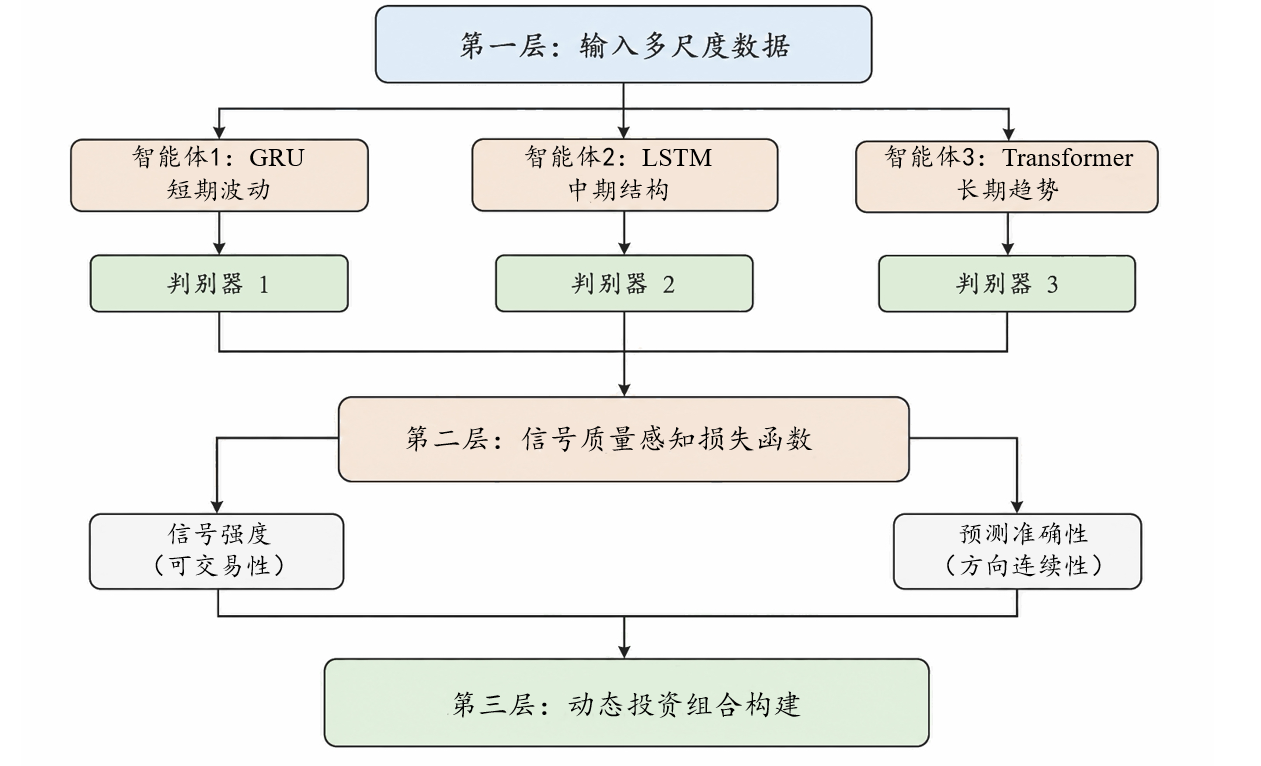
\includegraphics[width=0.8\textwidth]{figures/chap3/KDJ架构.png}
    \caption{GCA 多智能体群组交叉对抗整体框架示意图}
    \label{fig:MGCA-architecture}
\end{figure}

在这个多智能体系统中，GCA不再将多个模型视为静态集成，而是通过生成器与判别器之间的交叉评估来组织动态博弈。在真实金融市场中，算法交易已经深度影响市场流动性与交易过程，因而模型间交互不能简单视为静态预测器组合\cite{hendershott2011algorithmic}。在该系统中，多个异构生成器智能体基于各自的归纳偏置，对数据模式进行差异化刻画；多个判别器智能体则通过跨生成器的交叉评估机制，对生成结果在分布层面的合理性进行持续约束。生成器、判别器与元权重调节机制相互配合，共同推动多智能体系统向更加稳健的均衡状态演化。

形式化地，GCA核心机制由异构生成器集合$\mathcal{G}$与判别器集合$\mathcal{D}$构成：
\[
\mathcal{G} = \{G_1, G_2, \dots, G_N\}, \quad
\mathcal{D} = \{D_1, D_2, \dots, D_N\}.
\]
与经典生成对抗网络中“一对一”的生成器—判别器配对方式不同，本框架采用全连接的多对多博弈拓扑结构。通过引入端到端可微的元学习权重网络（Meta-weight Network），模型能够在训练过程中动态融合不同异构生成器输出，并调节子网络之间的相互作用强度，从而在多资产收益预测与组合权重生成之间建立更稳定的映射关系。


本章的整体方法对象是面向投资组合管理的GCA机制。GCA通过异构模型之间的交叉对抗学习，实现多尺度信息整合与分布正则化，避免模型趋同与模式崩塌，并将多模型输出进一步转化为投资组合管理所需的资产配置依据。为保持章节边界清晰，逆向师生蒸馏和孪生对抗自体再生在本章中不作为独立方法展开，也不被表述为本章的主体创新；它们仅作为GCA训练流程可接入的知识传递与状态修复接口，用于在消融实验中观察辅助机制对训练稳定性和组合表现的边际影响。
在这一结构中，多个异构智能体通过分组协同与交叉评估进行对抗学习，使生成器输出在数值精度和分布一致性之间形成约束。由此，本章方法的核心仍是“多资产预测信号如何转化为组合权重”，而不是提前展开后续章节的机制设计。

在上述整体架构下，本章进一步给出群组交叉对抗学习方法的训练流程。该流程包括初始化与预热、宏观演化与组间对抗、以及可选接口配置三个层次，分别对应模型启动、跨组竞争和辅助配置记录。这样安排的目的，是把GCA自身的训练主线和后续章节机制的接口位置区分开来，避免将本章写成多个创新模块的并列介绍。
GCA训练流程如算法 \ref{alg:MGCA_init}、\ref{alg:MGCA_evolution}、\ref{alg:MGCA_optional} 所示，其中GCA预热与组间对抗构成核心训练阶段，逆向师生蒸馏和孪生对抗自体再生仅作为可选辅助接口。

这里的“生成器”实际上充当的是“预测模型”的角色。将其称为“生成器”是为了将其纳入“对抗学习”的框架中，但其本质任务是条件预测。本文的核心目标不是生成逼真的假数据（如图像生成），而是生成鲁棒的投资组合权重。为了实现这一目标，模型需要先“生成”对未来收益的预测。在金融时序预测中，将模型视为生成器（生成未来的预测值）是一种常见的变通做法，尤其是在时间序列预测GAN的变体中。
判别器的输入是 (输入序列, 输出序列) 的组合。目标是判别器试图区分真实样本和生成样本。判别器的逻辑变为它不是在判断输出序列是真是假，而是在判断 “给定输入序列，输出序列这个组合是否符合真实市场的联合分布”。

结合上述分析，GCA 框架对生成器输出（预测收益率）的期待是双重的：
首先在数值上的准确性上，输出序列应该尽可能接近真实的未来收益率（由 LMSEL MSE保证）。
其次在分布上的一致性上（Distribution Consistency）：输出序列与输入 序列的联合分布应该无法与真实数据区分开（由 LadvL adv保证）。最终目标（Portfolio Management）是为了最终的夏普比率最大化（ LSharpeL Sharpe ）。文档 2.3.3 明确指出，优化目标是最大化夏普比率，这意味着模型不仅要预测方向，还要控制风险（波动率）。

\begin{algorithm}[H]
\caption{GCA 框架初始化与预热}
\label{alg:MGCA_init}
\begin{algorithmic}[0]
\Require 训练集 $\mathcal{D}_{\text{train}}$，验证集 $\mathcal{D}_{\text{val}}$；生成器集合 $\mathcal{G}$，判别器集合 $\mathcal{D}$
\Ensure 预热后的生成器集合 $\mathcal{G}$
\Statex
\State \textbf{初始化：} 随机初始化 $\mathcal{G}$ 和 $\mathcal{D}$，配置 Adam 优化器；创建多尺度滑动窗口数据集
\Statex
\State \textbf{Stage 1：组内交叉对抗（GCA）预热}
\For{epoch $= 1$ to $N_{\text{pretrain}}$}
    \For{each batch $(x^{(i)}, y) \in \mathcal{D}_{\text{train}}$, $i = 1 \ldots N$}
        \State 生成器前向：$\hat{y}_i \leftarrow G_i(x^{(i)})$
        \State \textbf{判别器训练：} 计算 $y$（标签 1）与 $\hat{y}_i$（标签 0）的二元交叉熵，更新 $D_i$
        \State \textbf{生成器训练：}
        \State $\quad \mathcal{L}_{\text{task}} \leftarrow \sum_{i=1}^N \lambda_i^{\text{task}} \cdot \text{MultiTaskLoss}(G_i(x^{(i)}), y)$
        \State $\quad \mathcal{L}_{\text{adv}} \leftarrow \sum_{i=1}^N \lambda_i^{\text{gan}} \cdot \left[-\log D_i(x^{(i)}, \hat{y}_i)\right]$
        \State $\quad \mathcal{L}_{\text{sharpe}} \leftarrow \lambda_{\text{sharpe}} \cdot \text{SharpeLoss}(\{\hat{y}_i\})$
        \State $\quad \mathcal{L}_G \leftarrow \lambda_{\text{mse}}\mathcal{L}_{\text{task}} + \lambda_{\text{gan}}\mathcal{L}_{\text{adv}} + \lambda_{\text{sharpe}}\mathcal{L}_{\text{sharpe}}$
        \State $\quad$ 使用 $\mathcal{L}_G$ 更新 $\mathcal{G}$
    \EndFor
\EndFor
\State \Return $\mathcal{G}$
\end{algorithmic}
\end{algorithm}

\begin{algorithm}[H]
\caption{GCA 框架宏观演化与组间对抗}
\label{alg:MGCA_evolution}
\begin{algorithmic}[0]
\Require 预热后的生成器集合 $\mathcal{G} = \{G_i\}$，判别器集合 $\mathcal{D} = \{D_i\}$，验证集 $\mathcal{D}_{\text{val}}$
\Ensure 全局最优生成器 $G^{\star}$
\Statex
\State \textbf{Stage 2：宏观演化循环 — 组内选拔与蒸馏}
\For{global\_epoch $= 1$ to $N_{\text{global}}$}
    \For{inner\_epoch $= 1$ to $N_{\text{inner}}$}
        \State 在 $\mathcal{D}_{\text{val}}$ 上评估：
        \State $\quad G_i^{\star} \leftarrow \arg\min_{G_i} \text{MSE}(G_i)$
        \State $\quad D_i^{\star} \leftarrow \arg\min_{D_i} \text{CE}(D_i)$
        \State 在组内执行一对一 生成对抗网络 对抗训练与知识蒸馏（蒸馏项：均方误差(Logits) + 均方误差(Features)）
    \EndFor
\EndFor
\Statex
\State \textbf{Stage 3：组间对抗 — 跨组竞争收敛}
\For{outer\_epoch $= 1$ to $N_{\text{outer}}$}
    \State 在 $\mathcal{D}_{\text{val}}$ 上选取最优生成器与判别器：
    \State $\quad G^{\dagger} \leftarrow \arg\min_{G_i^{\star}} \text{MSE}(G_i^{\star})$
    \State $\quad D^{\dagger} \leftarrow \arg\min_{D_i^{\star}} \text{CE}(D_i^{\star})$
    \State 在 $G^{\dagger}$ 与 $D^{\dagger}$ 之间执行组间 生成对抗网络 对抗训练
\EndFor
\Statex
\State 在 $\mathcal{D}_{\text{val}}$ 上评估：$G^{\star} \leftarrow \arg\min_G \text{MSE}(G)$
\State \Return $G^{\star}$
\end{algorithmic}
\end{algorithm}

\begin{algorithm}[H]
\caption{GCA 框架可选接口配置}
\label{alg:MGCA_optional}
\begin{algorithmic}[0]
\Require GCA训练输出 $G^{\star}$，候选生成器集合 $\{G_i\}$，验证集 $\mathcal{D}_{\text{val}}$
\Ensure 消融实验中的接口配置
\State 以GCA训练流程作为主配置，记录基准表现
\If{启用知识传递接口}
    \State 将该接口作为消融配置接入GCA训练结果
    \State 仅记录其对收益、回撤和换手率的边际影响；具体机制在后续章节展开
\EndIf
\If{启用状态修复接口}
    \State 将该接口作为消融配置接入GCA训练结果
    \State 仅记录其对模型稳定性和组合表现的边际影响；具体机制在后续章节展开
\EndIf
\State \Return 不同接口配置下的GCA模型结果
\end{algorithmic}
\end{algorithm}


在时间复杂度方面，算法1的单次迭代复杂度主要来源于生成器与判别器的前向传播和反向传播。设生成器/判别器的数量为 $N$，批次大小为 $B$，时间窗口长度为 $T$，隐藏层维度为 $d$，则单个生成器的前向传播复杂度为 $O(T^2 \cdot d)$（针对自注意力序列模型）或 $O(T \cdot d^2)$（针对循环神经网络架构）。综合考虑多生成器并行训练的场景，算法1每轮迭代的总时间复杂度为 $O(N \cdot B \cdot (T^2 \cdot d + T \cdot d^2))$。若预训练轮数为 $N_{\text{pretrain}}$，每轮包含 $N_{\text{batch}}$ 个批次，则算法1的总时间复杂度为 $O(N_{\text{pretrain}} \cdot N_{\text{batch}} \cdot N \cdot B \cdot (T^2 \cdot d + T \cdot d^2))$。在实际应用中，由于 $N_{\text{batch}} = |\mathcal{D}_{\text{train}}| / B$，该复杂度与训练集规模呈线性关系。

算法2在算法1的基础上增加了组内选拔蒸馏与组间对抗两个阶段。设组内蒸馏轮数为 $N_{\text{inner}}$，组间对抗轮数为 $N_{\text{outer}}$，全局演化轮数为 $N_{\text{global}}$。组内蒸馏阶段需要对每个生成器在验证集上进行评估，其复杂度为 $O(N \cdot |\mathcal{D}_{\text{val}}| \cdot (T^2 \cdot d + T \cdot d^2))$，随后执行的一对一生成对抗网络对抗训练与知识蒸馏的复杂度与算法1相当。组间对抗阶段仅对选出的最优生成器与判别器进行训练，其复杂度为 $O(N_{\text{outer}} \cdot B \cdot (T^2 \cdot d + T \cdot d^2))$，较组内阶段显著降低。因此，算法2的总时间复杂度约为 $O(N_{\text{global}} \cdot N_{\text{inner}} \cdot N \cdot |\mathcal{D}_{\text{val}}| \cdot (T^2 \cdot d + T \cdot d^2) + N_{\text{outer}} \cdot B \cdot (T^2 \cdot d + T \cdot d^2))$。验证集评估的复杂度在实际中通常低于训练前向传播，因为该过程无需进行梯度计算与参数更新。

算法3仅用于说明GCA训练流程可以接入知识传递与状态修复接口。逆向师生蒸馏和孪生对抗自体再生在本章中不作为独立展开的主体机制，而是作为消融实验中的可选配置，用于观察辅助接口在稳定训练和异常修复方面的边际作用。其具体算法细节将在后续章节结合相应任务展开。

在空间复杂度方面，以GCA为核心的多智能体对抗方法的主要存储开销包括模型参数存储、激活值存储、优化器状态存储以及数据存储四个部分。设单个生成器的参数量为 $|\theta_G|$，单个判别器的参数量为 $|\theta_D|$，则模型参数存储的空间复杂度为 $O(N \cdot (|\theta_G| + |\theta_D|))$。在前向传播过程中，需要存储各层的中间激活值用于反向传播，其空间复杂度为 $O(N \cdot B \cdot T \cdot d)$。若采用Adam优化器，需要为每个参数维护一阶矩和二阶矩，优化器状态的存储开销为模型参数的两倍，即 $O(2N \cdot (|\theta_G| + |\theta_D|))$。此外，训练数据和验证数据需要加载至内存，其空间复杂度为 $O(|\mathcal{D}_{\text{train}}| \cdot T \cdot F + |\mathcal{D}_{\text{val}}| \cdot T \cdot F)$，其中 $F$ 为特征维度。

从整体框架的复杂度特征来看，GCA训练流程的时间复杂度主要由算法1和算法2中的前向传播与反向传播决定，与生成器数量 $N$、训练集规模 $|\mathcal{D}_{\text{train}}|$ 以及模型深度 $(T^2 \cdot d)$ 呈线性或近似线性关系。空间复杂度则主要受模型参数量和批次大小影响。相较于传统的单生成器-单判别器生成对抗网络框架，该流程引入了 $N$ 倍的计算和存储开销，但通过并行化训练和验证集评估的优化，该开销在实际部署中处于可接受范围内。算法3中的可选接口只用于说明框架可扩展性，其细节不作为本章展开重点。







%\subsection{评估指标体系}

%为了全面量化多智能体群组交叉对抗框架在金融场景下的有效性，我们构建了一个涵盖收益性、风险性和交易成本的多维评估体系:

% \subsubsection{风险调整后收益}

%\paragraph{1.风险调整后收益}
%此类指标衡量单位风险敞口下的超额回报，是评估策略鲁棒性的核心标准。
 
%\begin{itemize}
   % \item \textbf{夏普比率 (Sharpe Ratio)}：定义为超额收益的期望与标准差之比。高夏普比率意味着策略位于有效前沿（Efficient Frontier）的更优位置。
   % \item \textbf{卡玛比率 (Calmar Ratio)}：定义为年化收益率与最大回撤之比，衡量策略在极端市场环境下的修复能力。
%\end{itemize}

% \subsubsection{绝对收益与稳定性特征}
%\paragraph{2.绝对收益与稳定性特征}
%\begin{itemize}
    %\item \textbf{年化收益率 (AnnRet)}：直观反映了策略的财富积累速度。
   % \item \textbf{最大回撤 (MDD)}：描述了资金曲线从峰值的最大跌幅，量化了策略的尾部风险。
%\end{itemize}

% \subsubsection{交易行为特征}
%\paragraph{3.交易行为特征}
%\begin{itemize}
    %\item \textbf{胜率 (Win Rate)}：盈利交易占比。
    %\item \textbf{平均换手率 (Average Turnover)}：反映了策略的交易频率。在考虑交易成本（Transaction Costs）和滑点（Slippage）的现实环境中，低换手率是防止利润被摩擦成本侵蚀的关键因素。
%\end{itemize}



上述说明限定了辅助接口在本章中的位置。后续实验以GCA为主方法，在统一回测框架下观察其对不同资产组合配置效果的影响，并在消融设置中报告辅助接口的边际作用。

\section{实验}

本节在统一的数据划分、回测规则与评价指标下检验GCA在投资组合管理任务中的表现。实验围绕“多资产收益预测—组合权重生成—风险收益评估”展开，重点观察GCA能否改善多资产配置中的风险调整后收益，并降低单一模型在不同市场状态下的配置偏差。因此，本节不把实验结果简单解释为预测精度提升，也不把辅助接口的边际效果上升为本章主体贡献，而是结合权重生成质量、回撤控制和组合层面表现分析GCA是否真正服务于投资组合管理。

为了将投资组合管理中的预测信号转化为可执行的资产权重，我们将生成器的输出通过稳健的策略函数转化为实际仓位。早期交易系统研究已经指出，交易模型应直接围绕投资绩效函数进行优化，而不仅是最小化预测误差\cite{moody1998performance}。这一观点与本章方法目标一致：模型输出只有转化为仓位并接受收益、风险和交易约束检验，才具有投资组合管理意义。

本章采用连续多空策略，将预测信号映射为资产权重。直接强化学习交易研究表明，将预测信号直接映射为交易动作或仓位决策，有助于弥合统计预测与交易执行之间的距离\cite{moody2001learning}：
\begin{equation}
    w_{i,t} = \frac{\hat{r}_{i,t} - \bar{r}_t}{\sum_{j} |\hat{r}_{j,t} - \bar{r}_t|}
\end{equation}
其中 $\bar{r}_t$ 为截面均值。该策略实现了资金的中性化配置（Dollar Neutral），即 $\sum w_{i,t} = 0$，专注于捕捉资产间的相对强弱关系（阿尔法），而非市场的系统性风险（贝塔）。

%\subsection{交易执行与回测框架}

为说明模型输出如何进入样本外回测，本文采用统一的交易执行与回测框架。算法交易研究强调，预测信号只有在执行机制与市场微观结构约束下转化为真实订单后，才具有完整的经济意义\cite{cartea2015algorithmic}。模型生成的分类预测经 softmax 归一化后得到三类信号概率 $(p_0, p_1, p_2)$，分别对应做空、持有、做多的概率。取 $\max(p_0, p_2)$ 作为置信度权重 $w_t \in [0,1]$，再根据预测类别 $a$ 确定方向，计算策略每日收益率：
\[
w_t = \max(p_0, p_2), \qquad
r_t^{\text{strategy}} =
\begin{cases}
  +w_t \cdot r_t, & a = 2 \text{（做多）} \\
  -w_t \cdot r_t, & a = 0 \text{（做空）} \\
  0, & a = 1 \text{（持有）}
\end{cases}
\]
其中 $r_t = (P_t - P_{t-1}) / P_{t-1}$ 为基础价格变化率。策略不涉及保证金制度或杠杆，$w_t$ 即为实际名义敞口比例（最大为 1，即满仓）。

\textbf{Equity 曲线与累计收益}：Equity 曲线以 $1.0$ 为起点，通过逐日复利累乘计算：
\[
\text{equity}_t = \prod_{i=1}^{t}\left(1 + r_i^{\text{strategy}}\right).
\]
累计收益率和年化收益率即在此 equity 曲线的基础上计算得到。

\textbf{投资策略评估指标}：为评估交易策略在样本外回测中的表现，本框架采用包含风险、收益和交易摩擦的多维指标体系：
\begin{itemize}
    \item \textbf{风险调整后收益}：\textbf{夏普比率}，用于衡量单位风险下的超额收益能力。夏普关于基金绩效评价的经典研究为风险调整收益度量提供了早期依据\cite{sharpe1966mutual}。
    \item \textbf{收益表现}：\textbf{总收益率} 和 \textbf{年化收益率}。
    \item \textbf{风险控制}：\textbf{年化波动率} 和 \textbf{最大回撤}，以评估策略的稳定性与尾部风险。
    \item \textbf{交易特征}：\textbf{胜率} 和 \textbf{平均换手率}，用于反映信号的准确度及策略的交易成本敏感性。
\end{itemize}
此外，通过累计收益率曲线展示不同模型在样本外测试期间的净值变化和回撤修复情况。





%\section{实验数据与评估指标}

%\subsection{数据与实验设置}



%\subsection{实验数据与评估指标}
%\subsection{组合指数的构建}


%\subsubsection{QR 指标的定义}

%\subsubsection{实验组合设计}

% \section{实验组合设计}
为检验GCA机制在不同市场结构下的投资组合管理能力，本章以多资产组合配置作为实验对象，基于经济板块逻辑与资产间的相关性结构，构建了六类具有差异化市场特征的投资组合（P1--P6），如表~\ref{tab:portfoliosAligned}所示。该实验设计的目的不是验证单一资产预测效果，而是观察GCA在不同资产相关结构、不同数据长度和不同波动环境下，能否保持相对稳定的权重生成能力与风险调整收益表现：

% \begin{itemize}
%     \item \textbf{P1：宏观敏感型组合}（黄金、原油、铜、豆粕）——涵盖贵金属、能源与农产品，资产间受宏观经济周期与地缘政治事件驱动，旨在检验模型对突发状态切换的适应能力。
%     \item \textbf{P2：农产品周期组合}（玉米、豆粕、白糖、棉花）——受季节性供需与自然因素影响，具有显著的周期性与均值回归特征，用于验证模型对长期依赖的捕捉能力。
%     \item \textbf{P3：能源-化工链条组合}（原油、甲醇、聚丙烯、PTA）——上下游产业链资产，存在因果时滞与波动率传导效应，用于测试模型对跨资产价格传导的结构化推理能力。
%     \item \textbf{P4：避险-风险对冲组合}（黄金、铜、原油、动力煤）——包含避险资产与周期性风险资产，在不同市场状态下呈现动态变化的相关结构，用于验证模型的多目标优化与动态对冲能力。
%     \item \textbf{P5：高波动技术交易组合}（PVC、甲醇、PTA、聚丙烯）——均为波动率较高的化工品种，收益分布呈厚尾特征，用于压力测试模型在极端行情下的风险适应性。
%     \item \textbf{P6：多元低相关组合}（黄金、棉花、铁矿石、白糖、动力煤）——跨越多个独立板块，资产间相关性较低，用于测试模型在低信噪比环境下的特征解耦能力与防过拟合能力。
% \end{itemize}

% {P1}是宏观敏感型组合（黄金、原油、铜、豆粕），这一类主要涵盖贵金属、能源与农产品，资产间受宏观经济周期与地缘政治事件驱动，旨在检验模型对突发状态切换的适应能力；
% {P2}是农产品周期组合（玉米、豆粕、白糖、棉花），这一类受季节性供需与自然因素影响，具有显著的周期性与均值回归特征，用于验证模型对长期依赖的捕捉能力；
% {P3}是能源-化工链条组合（原油、甲醇、聚丙烯、PTA），存在明显时滞与波动率传导效应，用于测试模型对跨资产价格传导的结构化推理能力；
% {P4}为避险-风险对冲组合（黄金、铜、原油、动力煤），资产在不同市场状态下呈现动态变化，以验证模型的多目标优化与动态对冲能力；
% {P5}为高波动技术交易组合（PVC、甲醇、PTA、聚丙烯），由波动率较高的化工品种组成，收益分布呈厚尾特征，用于压力测试模型在极端行情下的风险适应性；
% {P6}为多元低相关组合（黄金、棉花、铁矿石、白糖、动力煤），用于检验模型在低信噪比环境下的特征解耦能力与防过拟合能力。


上述组合在驱动因素、波动特征、相关结构及数据长度等维度上形成互补，用于观察GCA机制在宏观事件冲击、产业链传导、周期性波动及极端市场环境下的资产配置能力和组合风险控制能力。具体的资产配置与有效回测区间如表 \ref{tab:portfoliosAligned} 所示。

\begin{table}[htbp]
    \centering
    \caption{实验资产组合配置与有效对抗训练区间}
    \label{tab:portfoliosAligned}
    \resizebox{\textwidth}{!}{%
    \begin{tabular}{clll}
    \toprule
    \textbf{编号} & \textbf{组合名称} & \textbf{底层资产} & \textbf{有效区间} \\
    \midrule
    P1 & 宏观敏感型组合 & Gold, Crude Oil*, Copper, Soybean Meal & 2018.03 - 2024.12 \\
    P2 & 农产品核心组合 & Corn, Soybean Meal, Sugar, Cotton & 2006.01 - 2024.12 \\
    P3 & 能源-化工联动组合 & Crude Oil*, Methanol, PP, PTA & 2018.03 - 2024.12 \\
    P4 & 避险-风险对冲组合 & Gold, Copper, Crude Oil*, Thermal Coal & 2018.03 - 2024.12 \\
    P5 & 高波动技术交易组合 & PVC, Methanol, PTA, PP & 2014.02 - 2024.12 \\
    P6 & 多元低相关组合 & Gold, Cotton, Iron Ore, Sugar, Thermal Coal & 2013.10 - 2024.12 \\
    \bottomrule
    \end{tabular}%
    }
    \begin{tablenotes}
        \footnotesize
        \item[*] 注：带 * 号资产（如原油 SC）为该组合的“时间瓶颈”资产，限制了整体回测的起始点。这种差异化的时间窗口恰好允许我们评估模型在长周期（如 P2）与短周期（如 P1）不同数据丰度下的鲁棒性。
    \end{tablenotes}
\end{table}

该组合设计从三方面体现验证价值：一是数据丰度适应性检验上，P2近20年的完整周期数据可用于验证模型的收敛上限，P1、P4约6年数据用于测试小样本泛化能力；二是逻辑合理性，通过P3组合验证模型对产业链价格传导的捕捉能力；三是环境鲁棒性，利用P5高波动组合实现极端行情下的模型压力测试。

\subsection{实验数据集}
为服务多资产投资组合管理任务，本章构建了一个高维特征输入空间，用于同时刻画各资产自身的量价状态、资产之间的相对强弱关系以及组合配置所需的风险收益信息。金融深度学习基准研究表明，量价序列、订单流与技术指标等多维特征对于刻画市场微观结构具有重要意义\cite{ntakaris2018benchmark}。数据集不仅包含基础的量价数据（开盘价、最高价、最低价、收盘价与成交量），还通过特征工程构建了三大类技术指标：
% \begin{enumerate}
%     \item \textbf{趋势类指标}：包括多周期移动平均（MA5/15/30）与指数平滑异同移动平均（MACD），用于捕捉截面动量；
%     \item \textbf{震荡类指标}：包括相对强弱指数（RSI）与随机指标（KDJ），用于识别超买超卖的市场状态；
%     \item \textbf{波动类指标}：包括真实波幅（ATR）与布林带（Bollinger Bands），用于量化市场的不确定性边界。
% \end{enumerate}
趋势类指标包括多周期移动平均（MA5/15/30）与指数平滑异同移动平均线，用于捕捉截面动量；
震荡类指标包括相对强弱指数与随机指标，用于识别超买超卖的市场状态；
波动类指标包括真实波幅与布林带，用于量化市场的不确定性边界。

数据集的特征池包括：
\begin{itemize}
   
    \item 价格和成交量：开盘价、最高价、最低价、收盘价、平均价和成交量。
   
    \item 持仓量：当前未平仓且未结算或关闭的衍生品合约（期货或期权）总数。
    
    \item 移动平均线因子：5日、15日和30日简单移动平均线（MA5、MA15、MA30）。
   
    \item 差离值：12日和26日指数移动平均线之间的差值。
   
    \item 信号线：差离值的9日指数移动平均线。
 
    \item 指数平滑异同移动平均线：计算为 差离值 减去 信号线，反映趋势强度和方向。
    
    \item 真实波幅：14日窗口内的平均真实波幅，捕捉价格波动性。
   
    \item 布林带：使用20日移动平均线和2倍标准差构建，用于指示相对价格水平。
   
    \item 相对强弱指数：基于14日周期计算，用于捕捉动量。
    
    \item K, D, J：随机指标（Stochastic Oscillator）分量，捕捉价格动量和反转信号，其中 K 是9日随机值，D 是其3日移动平均值，J 是动量乖离。
\end{itemize}
所有特征在输入神经网络前均经过严格的 区间缩放标准化 处理。我们为每个资产 $i$ 的每个特征 $f$ 独立计算训练集的极值，将其映射至 $[0, 1]$ 区间：
\begin{equation}
    x^{(i,f)}_{norm} = \frac{x^{(i,f)} - \min(X_{train}^{(i,f)})}{\max(X_{train}^{(i,f)}) - \min(X_{train}^{(i,f)})}
\end{equation}
这种处理有效消除不同指标（如价格的 $10^3$ 量级与 指数平滑异同移动平均线 的 $10^{-1}$ 量级）之间的尺度差异，确保梯度下降过程的各向同性。
% \subsection{实验参数设置}
\subsection{实验设计}
为了捕捉多尺度的时间动态并获取宏观视野，本文采用5、10 、20三种递增的输入窗口，分别对应周度脉冲、双周度波段和月度结构特征。
数据预处理阶段，为了消除量纲差异并加速梯度收敛，对上述特征采用了区间缩放标准化，将其映射至 $[0, 1]$ 区间：
\begin{equation}
    x_{norm} = \frac{x - x_{min}}{x_{max} - x_{min}}
\end{equation}
其中统计量 $x_{min}, x_{max}$ 仅在训练集上计算，以严格避免前瞻性偏差。

数据集按照时间顺序进行划分，将前70\%的数据作为训练集用于优化模型参数，后30\%的数据作为测试集用于样本外评估。本章之所以不采用随机打乱划分，是因为投资组合管理任务具有明确的时间先后关系，模型在测试阶段只能利用历史信息形成预测与权重配置，而不能提前接触未来样本。金融回测研究表明，多重检验、过度试验和样本外失效是量化策略评估中需要重点防范的问题\cite{harvey2016backtesting}。对于本文而言，这一问题尤其需要注意，因为本章同时比较多类模型、输入窗口和消融配置，若实验设计缺少统一约束，局部最优结果可能被误判为方法本身的稳定优势。

在多模型比较场景中，若研究者反复尝试不同模型、参数或组合设定，容易出现由数据窥探导致的偶然优胜。White的Reality Check从数据窥探角度讨论了多模型检验下的偶然优胜风险\cite{white2000realitycheck}。这一思想提示本文，模型比较不能只关注某个配置在测试集上的最高收益，而应在统一数据划分、统一交易规则和统一评价指标下观察不同模型的整体表现。Hansen提出的superior predictive ability检验进一步针对预测模型比较中的数据窥探问题提出了改进方案\cite{hansen2005spa}。因此，本章在实验设计中尽量固定数据划分、输入窗口和评估指标，使模型差异主要来自方法结构本身，而不是来自反复试验带来的选择偏差。

此外，回测过拟合研究从投资策略选择角度说明，标准留出法并不总能充分识别样本外失效风险\cite{bailey2015pbo}。基于这一考虑，本文在训练集与测试集之间设置长度为 $L_{gap}=20$ 天（即最大输入窗口长度）的“隔离期”。该期间数据不参与梯度更新与回测评估，用于减少训练末期窗口信息对测试初期样本的干扰，从而在不改变原始时间顺序的前提下，降低前瞻性偏差对实验结论的影响。

\noindent\textbf{评价指标说明}\par
本章在样本外测试中统一采用风险调整后收益、收益表现、风险控制与交易特征四类指标。具体包括夏普比率、卡玛比率、累计收益率、年化收益率、年化波动率、最大回撤、胜率和平均换手率。其中，夏普比率与卡玛比率用于衡量单位风险下的收益能力，累计收益率与年化收益率反映绝对收益水平，年化波动率与最大回撤刻画风险暴露，胜率与平均换手率用于观察交易信号质量及交易摩擦敏感性。



\noindent\textbf{消融与对照组实验设计}\par
% \subsection{添加交叉对抗后的性能退化验证}

% 为全面验证各模块的独立贡献与交互效应，本章采用两条消融路径并行的策略。

本章构建统一消融实验基准，重点检验GCA在投资组合管理任务中的作用。除基准模型与GCA配置外，实验仅保留知识传递接口和状态修复接口两类辅助配置，用于观察它们对GCA训练稳定性和组合表现的边际影响。相关接口不在本章展开机制细节，其作用仅通过消融实验进行报告。

% 路径B的核心目的，是在各章应用语境中验证本章主要贡献确实解决了本章声称的问题，避免固定场景带来的偏差。该路径通过渐进式消融实验，逐项验证各机制的有效性。

% 本章节渐进消融表（6-7行）：
\begin{table}[htbp]
\centering
\caption{渐进消融实验}
\label{tab:ablation_chap3_local}
\small
\setlength{\tabcolsep}{6pt}
\renewcommand{\arraystretch}{1.18}
\begin{tabular}{@{}p{0.36\textwidth}ccc@{}}
\toprule
\textbf{实验} & \textbf{GCA} & \textbf{知识传递接口} & \textbf{状态修复接口} \\
\midrule
基准模型 & $\times$ & $\times$ & $\times$ \\
+ GCA & $\checkmark$ & $\times$ & $\times$ \\
+ GCA+知识传递接口 & $\checkmark$ & $\checkmark$ & $\times$ \\
+ GCA+知识传递接口+状态修复接口 & $\checkmark$ & $\checkmark$ & $\checkmark$ \\
\bottomrule
\end{tabular}
\end{table}

% 关键交互对比（3个）：
% \begin{itemize}
%     \item GCA+S2T：验证交叉对抗是否需要双向蒸馏配合
%     \item S2T+Twin：验证逆向师生蒸馏是否需要孪生对抗自体再生配合
% \end{itemize}

% \textbf{修正说明}：第3章使用三个主要贡献（GCA+S2T+Twin），消融实验验证各模块的独立贡献。

% 输出策略：正文展示路径B（叙事贴合痛点），附录给出路径A（提供统一基准与交互效应解释）

% \begin{table}[htbp]
% \centering
% \caption{消融实验结果汇总表}
% \label{tab:ablation_study}
% \resizebox{\textwidth}{!}{
% \begin{tabular}{cccccccc}
% \toprule
% \textbf{模块配置} & \textbf{夏普比率} & \textbf{总收益率} & \textbf{年化收益率} & \textbf{最大回撤} & \textbf{说明} \\
% \midrule
% Baseline & 0.22 & 13.64\% & 2.81\% & -27.60\% & 基线模型 \\
% GCA (无蒸馏) & 0.25 & 15.85\% & 3.27\% & -26.41\% & 去除组内/全局蒸馏 \\
% GCA+蒸馏 & 0.33 & 21.44\% & 4.42\% & -25.67\% & 去除交叉对抗 \\
% 完整 MGCA & 0.45 & 28.87\% & 5.95\% & -20.34\% & 完整框架 \\
% \bottomrule
% \end{tabular}}
% \end{table}

% \vspace{1em}
% \textit{注：消融实验在 P1 组合上验证各模块的独立贡献。}

% \subsection{多目标损失配置}

% \begin{table}[htbp]
% \centering
% \caption{多目标损失配置对比实验结果}
% \label{tab:loss_config_comparison}
% \resizebox{\textwidth}{!}{
% \begin{tabular}{cccccccc}
% \toprule
% \textbf{损失配置} & \textbf{夏普比率} & \textbf{累计收益} & \textbf{年化波动} & \textbf{最大回撤} & \textbf{说明} \\
% \midrule
% 仅 MSE & — & — & — & — & 基准配置 \\
% MSE + GAN & — & — & — & — & 加入对抗损失 \\
% MSE + Sharpe & — & — & — & — & 加入夏普损失 \\
% MSE + GAN + Sharpe (完整) & — & — & — & — & 完整配置 \\
% \bottomrule
% \end{tabular}}
% \end{table}

% \vspace{1em}
% \textit{注：多目标损失配置对比实验在 P2 组合上进行。}

训练采用渐进式消融实验验证各模块的增量贡献：
% \begin{enumerate}
%     \item 基准配置（Baseline）：采用单一的均方误差（MSE）作为损失函数，仅从统计层面约束预测的数值精度。
%     \item MGCA完整配置：在保留 MSE 作为基础锚点的同时，叠加了对抗损失（GAN Loss） 与 夏普比率损失（Sharpe Ratio Loss）。这种混合范式实现了三重优化：MSE 保证基础保真度，GAN 正则化防止过拟合，夏普损失则直接优化投资组合的风险调整后收益，从而在保证信号物理意义的同时最大化决策效用。
% \end{enumerate}
基准配置以单一均方误差作为损失函数，并从门控循环单元、长短期记忆网络和自注意力序列模型中选取最优模型作为对照；随后加入GCA，观察群组交叉对抗对投资组合配置效果的影响；最后仅以接口形式接入知识传递和状态修复配置，用于观察辅助机制的边际作用。

为比较GCA及其辅助配置的边际作用，本章设计三层对照组：

\textbf{第一层：单模型基线（验证单模型的局限性）}
% \begin{itemize}
%     \item GRU：门控循环单元
%     \item LSTM：长短期记忆网络
%     \item Transformer：自注意力机制
% \end{itemize}
分别训练门控循环单元，长短期记忆网络和自注意力序列模型对比其性能优劣以选取最优基线模型。


% \textbf{第二层：传统机器学习方法}
% \begin{itemize}
%     \item Random Forest：随机森林
%     \item XGBoost：梯度提升树
%     \item LightGBM：轻量级梯度提升
%     \item SVM：支持向量机
% \end{itemize}



\textbf{第二层：传统集成（验证传统集成的局限性）}
% \begin{itemize}
%     % \item Bagging：Bootstrap聚合的多个GRU
%     \item 简单平均：GRU+LSTM+Transformer的元学习集成
%     % \item AdaBoost：自适应提升
% \end{itemize}
使用简单平均的集成方法，门控循环单元+长短期记忆网络+自注意力序列模型的元学习集成以作为对比的基准模型。

\textbf{第三层：本章方法变体（验证各模块的边际贡献）}
分别是基准模型、基准模型+GCA、基准模型+GCA+知识传递接口，以及基准模型+GCA+知识传递接口+状态修复接口。该渐进式设置用于观察GCA核心机制及其辅助接口对组合配置流程的边际影响。
% \begin{itemize}
%     \item GCA：baseline+群组交叉对抗
%     \item GCA+S2T：群组交叉对抗+逆向师生蒸馏
%     \item GCA+S2T+Twin：前两者+孪生对抗自体再生
% \end{itemize}
% \textbf{第四层：多智能体基线（验证现有智能体框架的局限性）}
% \begin{itemize}
%     \item Multi-Agent RL（如MAPS）\cite{jiang2017deep}：独立训练的多智能体强化学习
%     \item DML \cite{zhang2018dml}：双向互学习（无对抗机制）
%     \item 标准GAN：单生成器单判别器
% \end{itemize}

% \textbf{第五层：GAN变种基线（验证 GAN 变体的局限性，基于文献综述[1]）}
% \begin{itemize}
%     \item \textbf{WGAN-GP}：Wasserstein GAN with Gradient Penalty，解决模式崩塌问题
%     \item \textbf{TTUR}：Two Time-Scale Update Rule，两时间尺度更新规则
%     \item \textbf{MGAN}：Multi-Generator GAN，多生成器+共享判别器，鼓励生成器学习不同模式
%     \item \textbf{MGO-GAN}：正交正则化去相关，强制生成器特征独立
%     \item \textbf{D2GAN}：Dual Discriminator GAN，双判别器（标准KL+反向KL）平衡质量与多样性
%     \item \textbf{Parallel Generators}：并行结构生成器，多生成器并行训练
%     \item \textbf{TimeGAN}：时序生成对抗网络，专门针对时间序列
%     \item \textbf{QuantGAN}：金融时间序列生成对抗网络
% \end{itemize}



% \textbf{公平性约束}：所有基线必须严格遵守同一backbone、同一训练预算、同一数据划分、同一seed集合，否则对照结论会被质疑。

% 参考文献：
% [1] 在生成对抗网络（GAN）训练中故意打破平衡：一项文献综述. AMiner, 2026.

% \section{可视化验证实验}

% % 为验证 多智能体群组交叉对抗框架是否真正解决了上述"静态权重失效"和"模型趋同"问题，本章设计了以下可视化验证实验。
% 为验证 多智能体群组交叉对抗框架是否有效及各模块的作用，本章设计了以下可视化验证实验。

% \vspace{0.3em}
% \noindent\textbf{实验1：模型多样性验证（针对"模型趋同"问题）}

% 目的：验证 GCA 对抗机制能否产生多样化的预测，避免模型趋同。

% % 方法：使用 t-SNE 方法对各生成器（GRU、LSTM、Transformer）的预测结果进行可视化降维，观察其分布差异。
% 方法：对各生成器（GRU、LSTM、Transformer）的预测结果进行可视化降维，观察其分布差异。

% 预期：经过 GCA 对抗训练后，各生成器的预测分布应更加分散，表明每个生成器学习到了不同的市场特征。

% % \vspace{0.3em}
% % \noindent\textbf{实验2：动态权重有效性验证（针对"静态权重"问题）}

% % 目的：验证元权重网络能否自适应市场状态。

% % 方法：绘制权重热力图，对比不同市场阶段（高波动期/低波动期）的权重分布。

% % 预期：在高波动期，Transformer 等擅长趋势建模的生成器权重应增加；在低波动期，GRU/LSTM 等擅长均值回归的生成器权重应增加。

% \vspace{0.3em}
% \noindent\textbf{实验2：知识蒸馏效果验证（针对"知识传承"问题）}

% 目的：验证蒸馏机制能否加速弱模型学习。

% 方法：绘制训练收敛曲线，对比有无蒸馏的模型性能差异。

% 预期：加入蒸馏后，落后的生成器应能更快收敛，且最终性能更高。

% \vspace{0.3em}
% \noindent\textbf{实验3：孪生对抗自体再生对比}

% 目的：验证孪生对抗自体再生机制能否改善预测效果。

% 方法：对比训练前后有无孪生对抗自体再生的模型性能差异。

% 预期：经过对抗训练后，模型输出的效果及回测结果展示应有明显改善。


\subsection{结果分析与讨论}
\noindent\textbf{GCA模型多样性验证}\par
% \begin{table}[htbp]
% \centering
% \caption{实验结果汇总表}
% \label{tab:experimental_results_summary}
% \resizebox{\textwidth}{!}{
% \begin{tabular}{cccccccc}
% \toprule
% \textbf{组合} & \textbf{模型} & \textbf{夏普比率} & \textbf{总收益} & \textbf{年化收益} & \textbf{最大回撤 } & \textbf{胜率} & \textbf{换手率}\\
% \midrule

% \multirow{5}{*}{\textbf{P1}} 
% &Baseline&0.2168  &13.64\% &2.81\%  & -27.60\% &49.63\% &0.0760\\
% &Baseline-GCA& 0.2474 & 15.85\% &  3.27\% & -26.41\% &49.63\% &0.0713\\ 
% &Baseline-GCA-S2T &-&-&-&-&-&-\\
% &Baseline-GCA-S2T-Twin&-&-&-&-&-&-\\
% \midrule
% \multirow{5}{*}{\textbf{P2}} 
% &Baseline &0.3652 & 60.61\% &3.64\% &-21.17\% &50.14\% &0.1538\\
% &Baseline-GCA&-0.1990 & -16.40\% & -0.99\% & -33.07\% & 49.9\% & 0.1859\\
% &Baseline-GCA-S2T & 0.6279 &105.73\% &6.35\% &-17.13\% & 51.03\% &0.0479\\
% &Baseline-GCA-S2T-Twin&0.6446 &108.61\% &6.53\%  &-16.51\% &50.86\% &0.0397\\
% \midrule
% \multirow{5}{*}{\textbf{P3}} 
% &Baseline &-0.2816 &-12.51\% & -2.58\%  &-31.25\% &48.41\% &0.1600 \\
% &Baseline-GCA& -0.0976 & -6.53\% & -1.35\%& -22.23\% & 48.98\% & 0.1220\\
% &Baseline-GCA-S2T&0.1936 &12.82\% &2.64\% &-17.54\% &49.71\% & 0.0838 \\
% &Baseline-GCA-S2T-Twin&0.5764 &38.91\% &8.02\% &-13.72\% &50.12\% & 0.0408\\
% \midrule
% \multirow{5}{*}{\textbf{P4}} &Baseline&  0.6926&40.33\% &15.31\% &-25.67\% & 49.70\% & 0.1287 \\
% &Baseline-GCA & 0.4158 & 24.14\% &  9.16\% & -29.29\% & 49.4\% &0.1164\\
% &Baseline-GCA-S2T&0.6814 &39.49\% &14.99\% &-24.23\% &48.49\% & 0.0638 \\
% &Baseline-GCA-S2T-Twin&0.7120&40.45\% &15.35\% &-23.95\% & 47.89\% & 0.0408\\
% \midrule
% \multirow{5}{*}{\textbf{P5}} &Baseline&-&-&-&-&-&-\\
% &Baseline-GCA &-0.2657 & -17.40\% & -1.98\% & -34.01\% & 48.96\% & 0.3665\\
% &Baseline-GCA-S2T&-&-&-&-&-&-\\
% &Baseline-GCA-S2T-Twin&-&-&-&-&-&-\\
% \midrule
% \multirow{5}{*}{\textbf{P6}} &Baseline&0.4917 &45.72\% &6.59\% &-16.17\% &52.00\% &0.0939\\
% &Baseline-GCA &0.3817 &35.09\% &5.06\% &-18.31\% & 51.32\% & 0.1120\\
% &Baseline-GCA-S2T&0.5613 &52.00\% &7.50\% &-13.61\% &51.37\% & 0.0751   \\
% &Baseline-GCA-S2T-Twin& 0.5234& 49.12\% & 7.08\% &-13.97\% &50.97\% & 0.0835\\

% \bottomrule
% \end{tabular}}
% \end{table}

% \vspace{1em}
% \textit{注：表中数据为样本外测试集结果，"—"表示未适用。}

为评估GCA架构在不同组合上的样本外表现，本节对比其与单一生成器基准模型（门控循环单元、长短期记忆网络、自注意力序列模型）在六大组合上的样本外性能，所有模型采用相同超参数，评价指标覆盖投资回报、风险控制与交易摩擦成本。这里的结果分析重点在于说明群组交叉对抗架构能否在不同市场结构下保持多智能体协同与风险约束能力，而不是单纯比较某一组合的收益高低。因此，以下分析将训练收敛性、组合层回测结果和权重动态变化放在同一评价框架中讨论。

% \subsubsection{模型训练收敛性分析}

为了探究异构模型在复杂金融流形上的优化效率，记录各模型在所有六个实验组合上的训练损失演化轨迹。图 \ref{MGCA框架的MSE训练损失图}、 \ref{GRU的MSE训练损失图}、 \ref{LSTM的MSE训练损失图}、 \ref{Transformer的MSE训练损失图}  展示了各模型均方误差项的收敛全过程。四幅图中六个子图的排列顺序保持一致，均按从左至右、从上至下依次对应 P1--P6 六类实验组合。
\begin{figure}[htbp] % [htbp] 是位置参数：这里(h)、页首(t)、页尾(b)、单独一页(p)
    \centering % 图片居中
    % width=\textwidth 表示图片宽度占满正文文本宽度
    % 如果在文件夹里，路径要是 figures/my_chart.png
    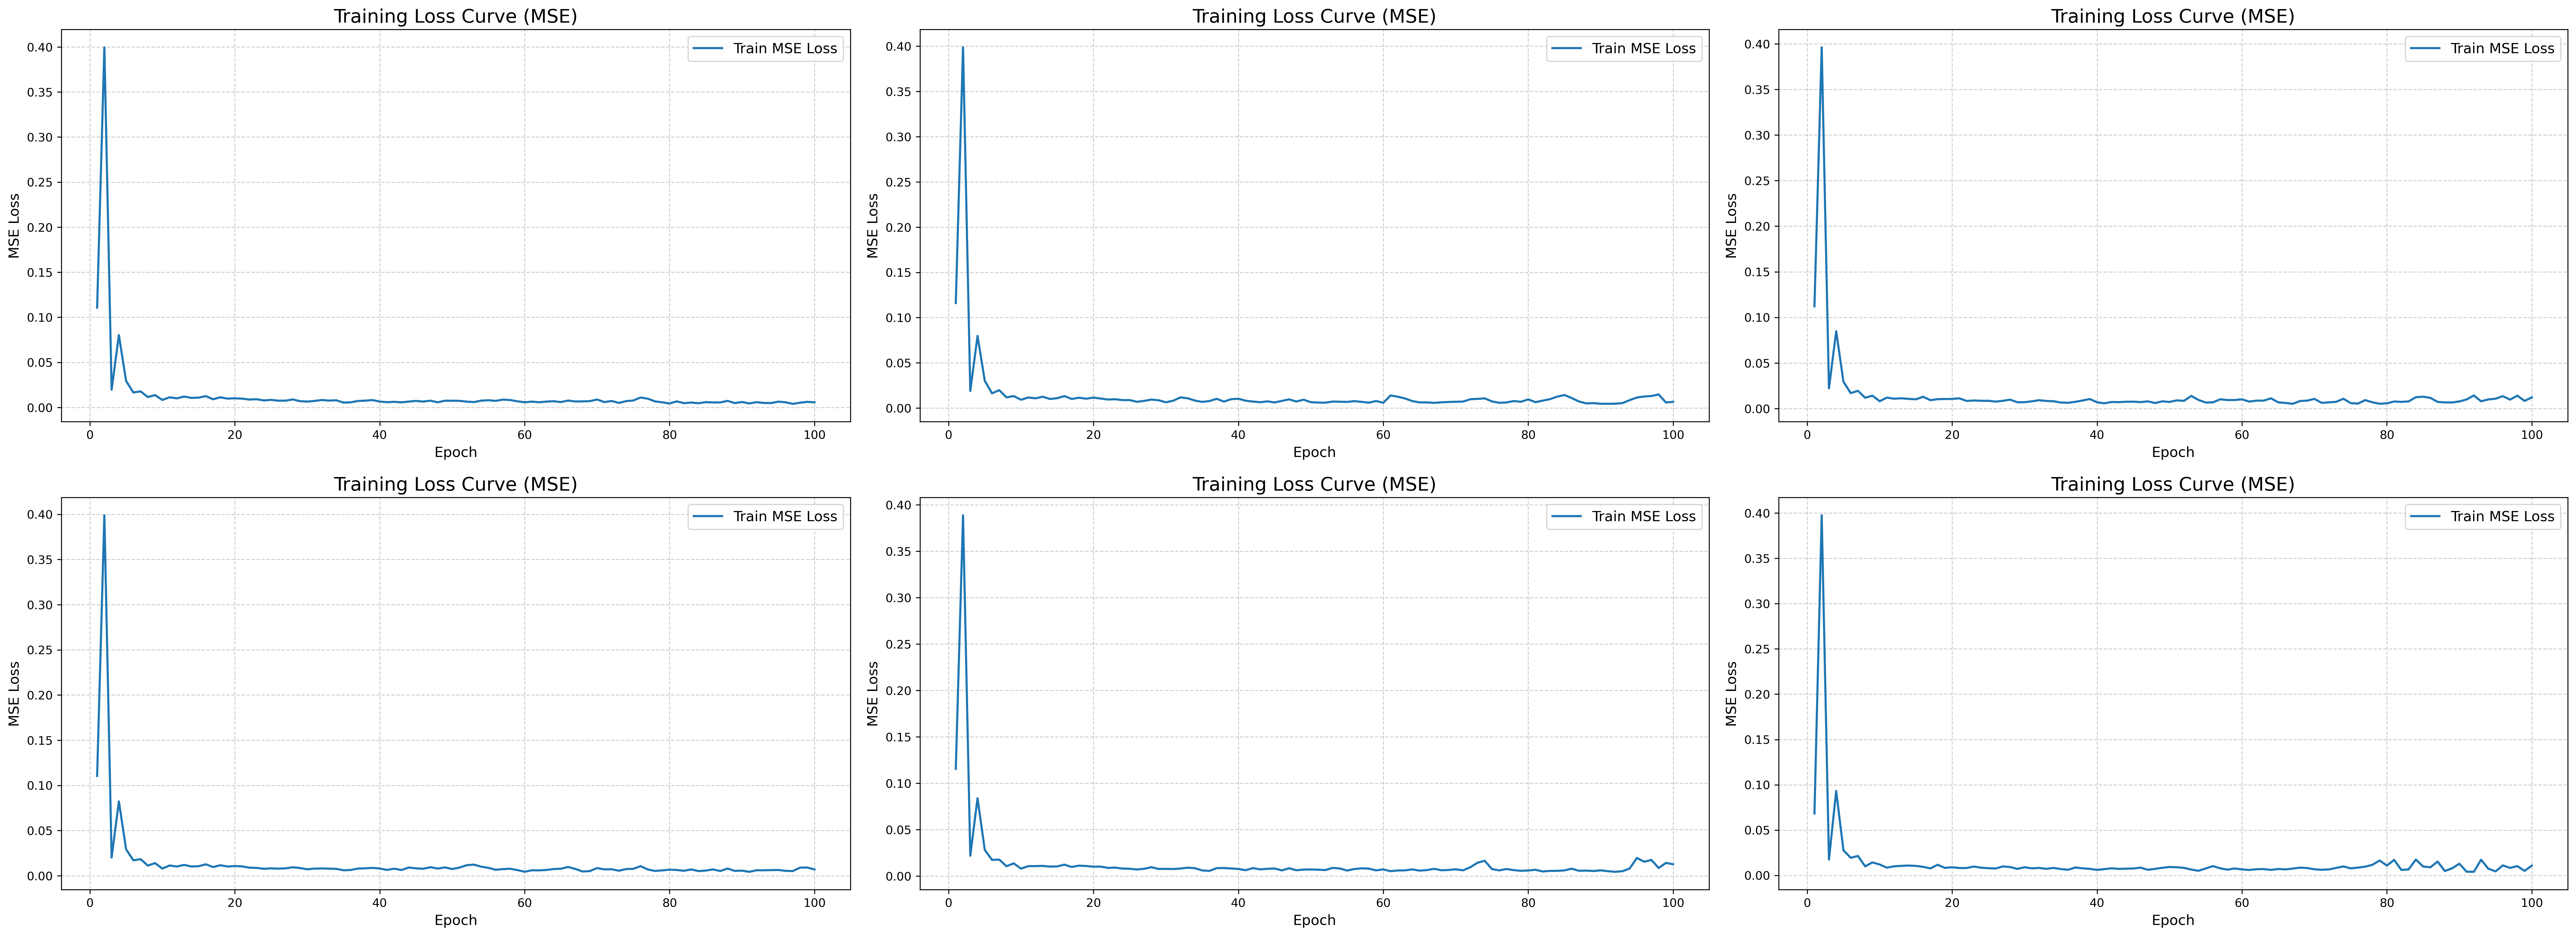
\includegraphics[width=0.8\textwidth]{figures/chap3/combined_MAA_mse_loss_curve.png} 
    \caption{GCA框架的均方误差训练损失图} % 图片下方的标题
    \label{MGCA框架的MSE训练损失图} % 【关键】设置引用标签，必须放在 \caption 之后！
\end{figure}

\begin{figure}[htbp] % [htbp] 是位置参数：这里(h)、页首(t)、页尾(b)、单独一页(p)
    \centering % 图片居中
    % width=\textwidth 表示图片宽度占满正文文本宽度
    % 如果在文件夹里，路径要是 figures/my_chart.png
    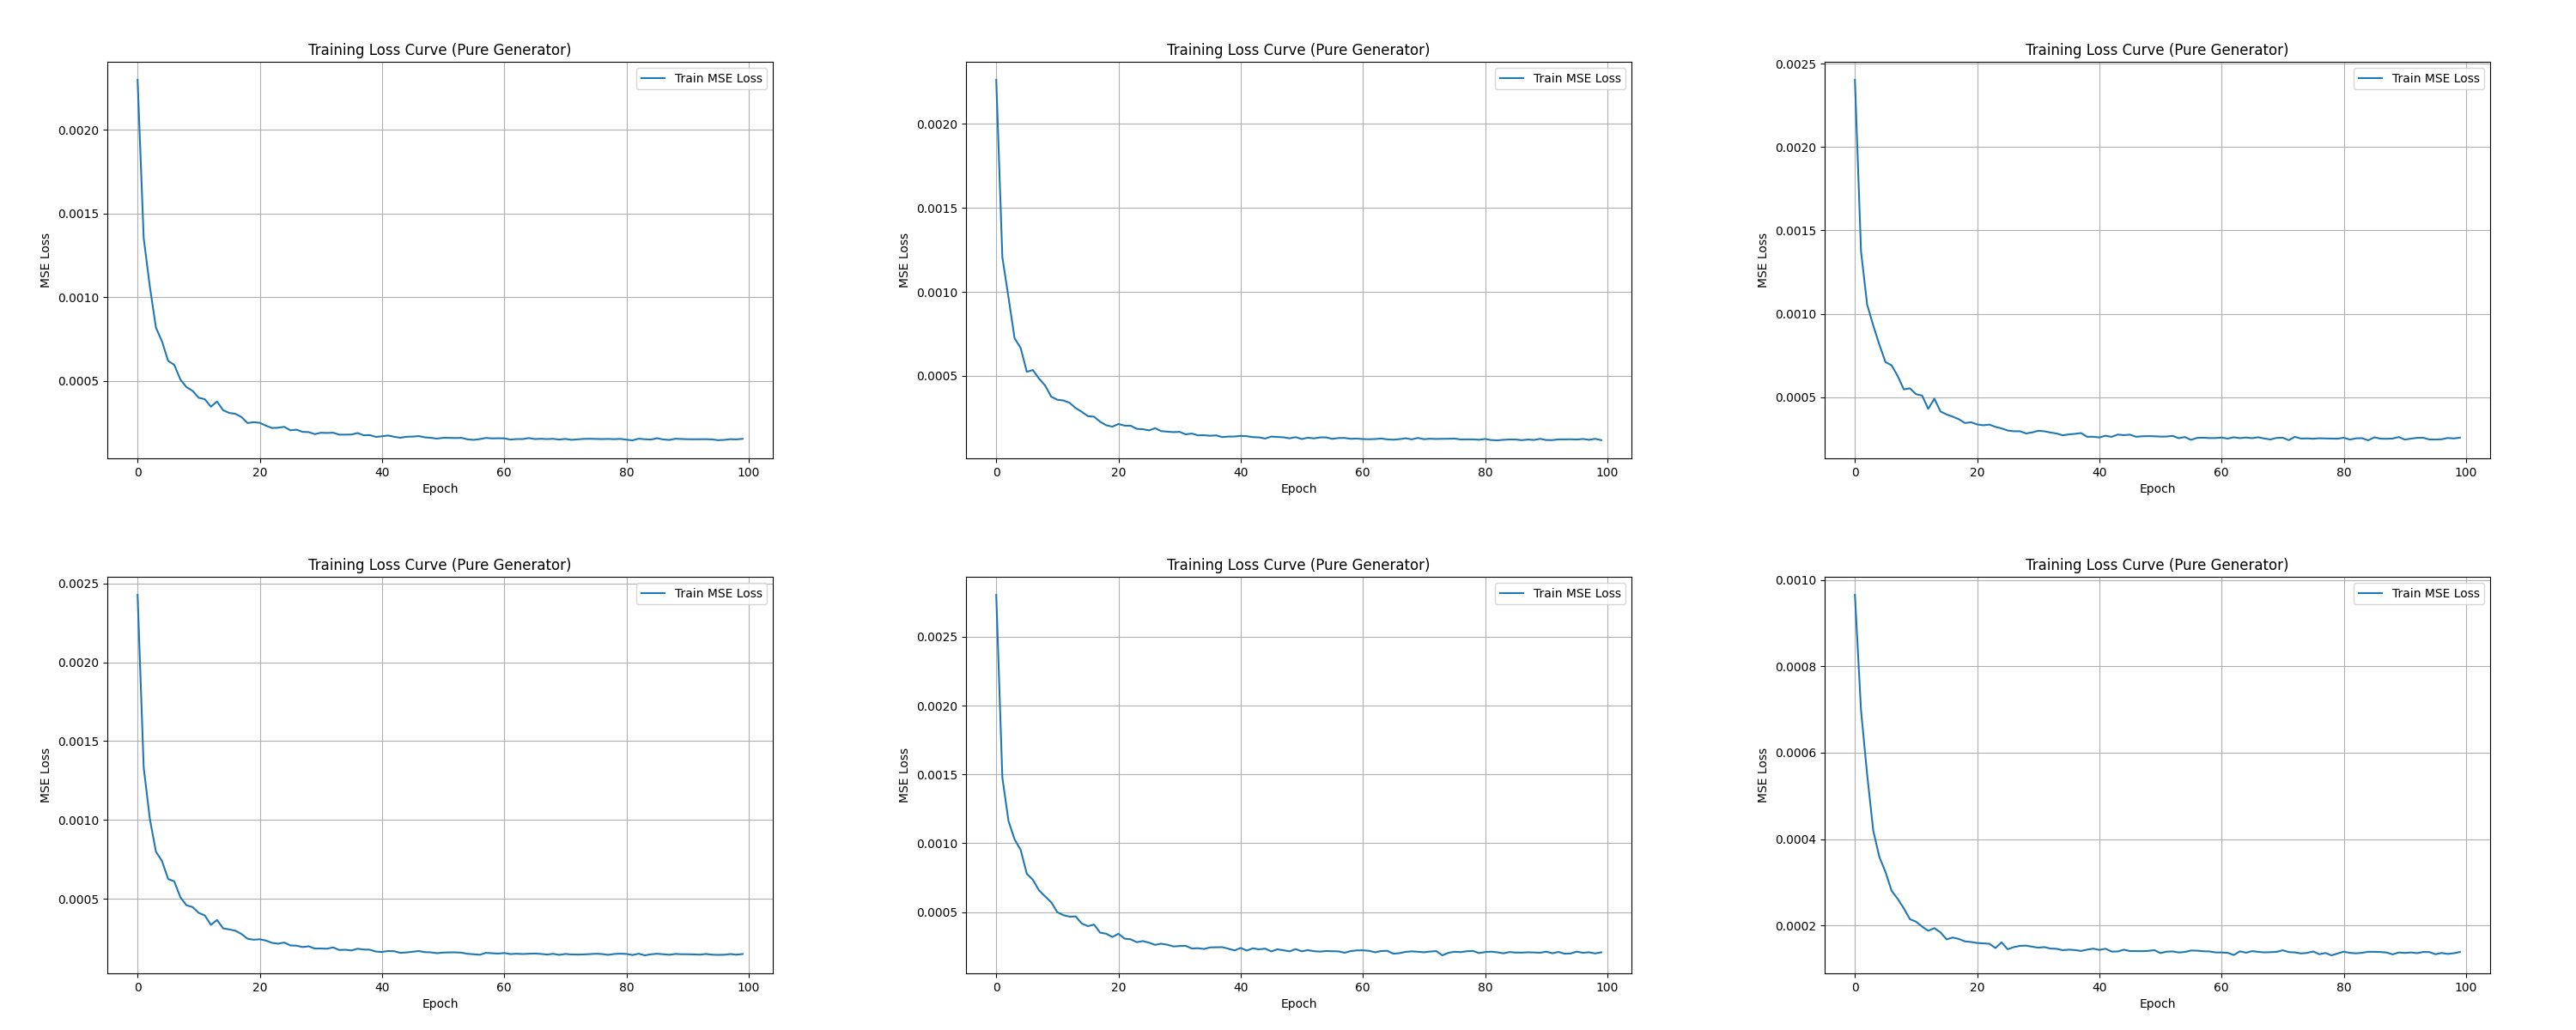
\includegraphics[width=0.8\textwidth]{figures/chap3/combined_GRU_mse_loss_curve.png} 
    \caption{门控循环单元的均方误差训练损失图} % 图片下方的标题
    \label{GRU的MSE训练损失图} % 【关键】设置引用标签，必须放在 \caption 之后！
\end{figure}

\begin{figure}[htbp] % [htbp] 是位置参数：这里(h)、页首(t)、页尾(b)、单独一页(p)
    \centering % 图片居中
    % width=\textwidth 表示图片宽度占满正文文本宽度
    % 如果在文件夹里，路径要是 figures/my_chart.png
    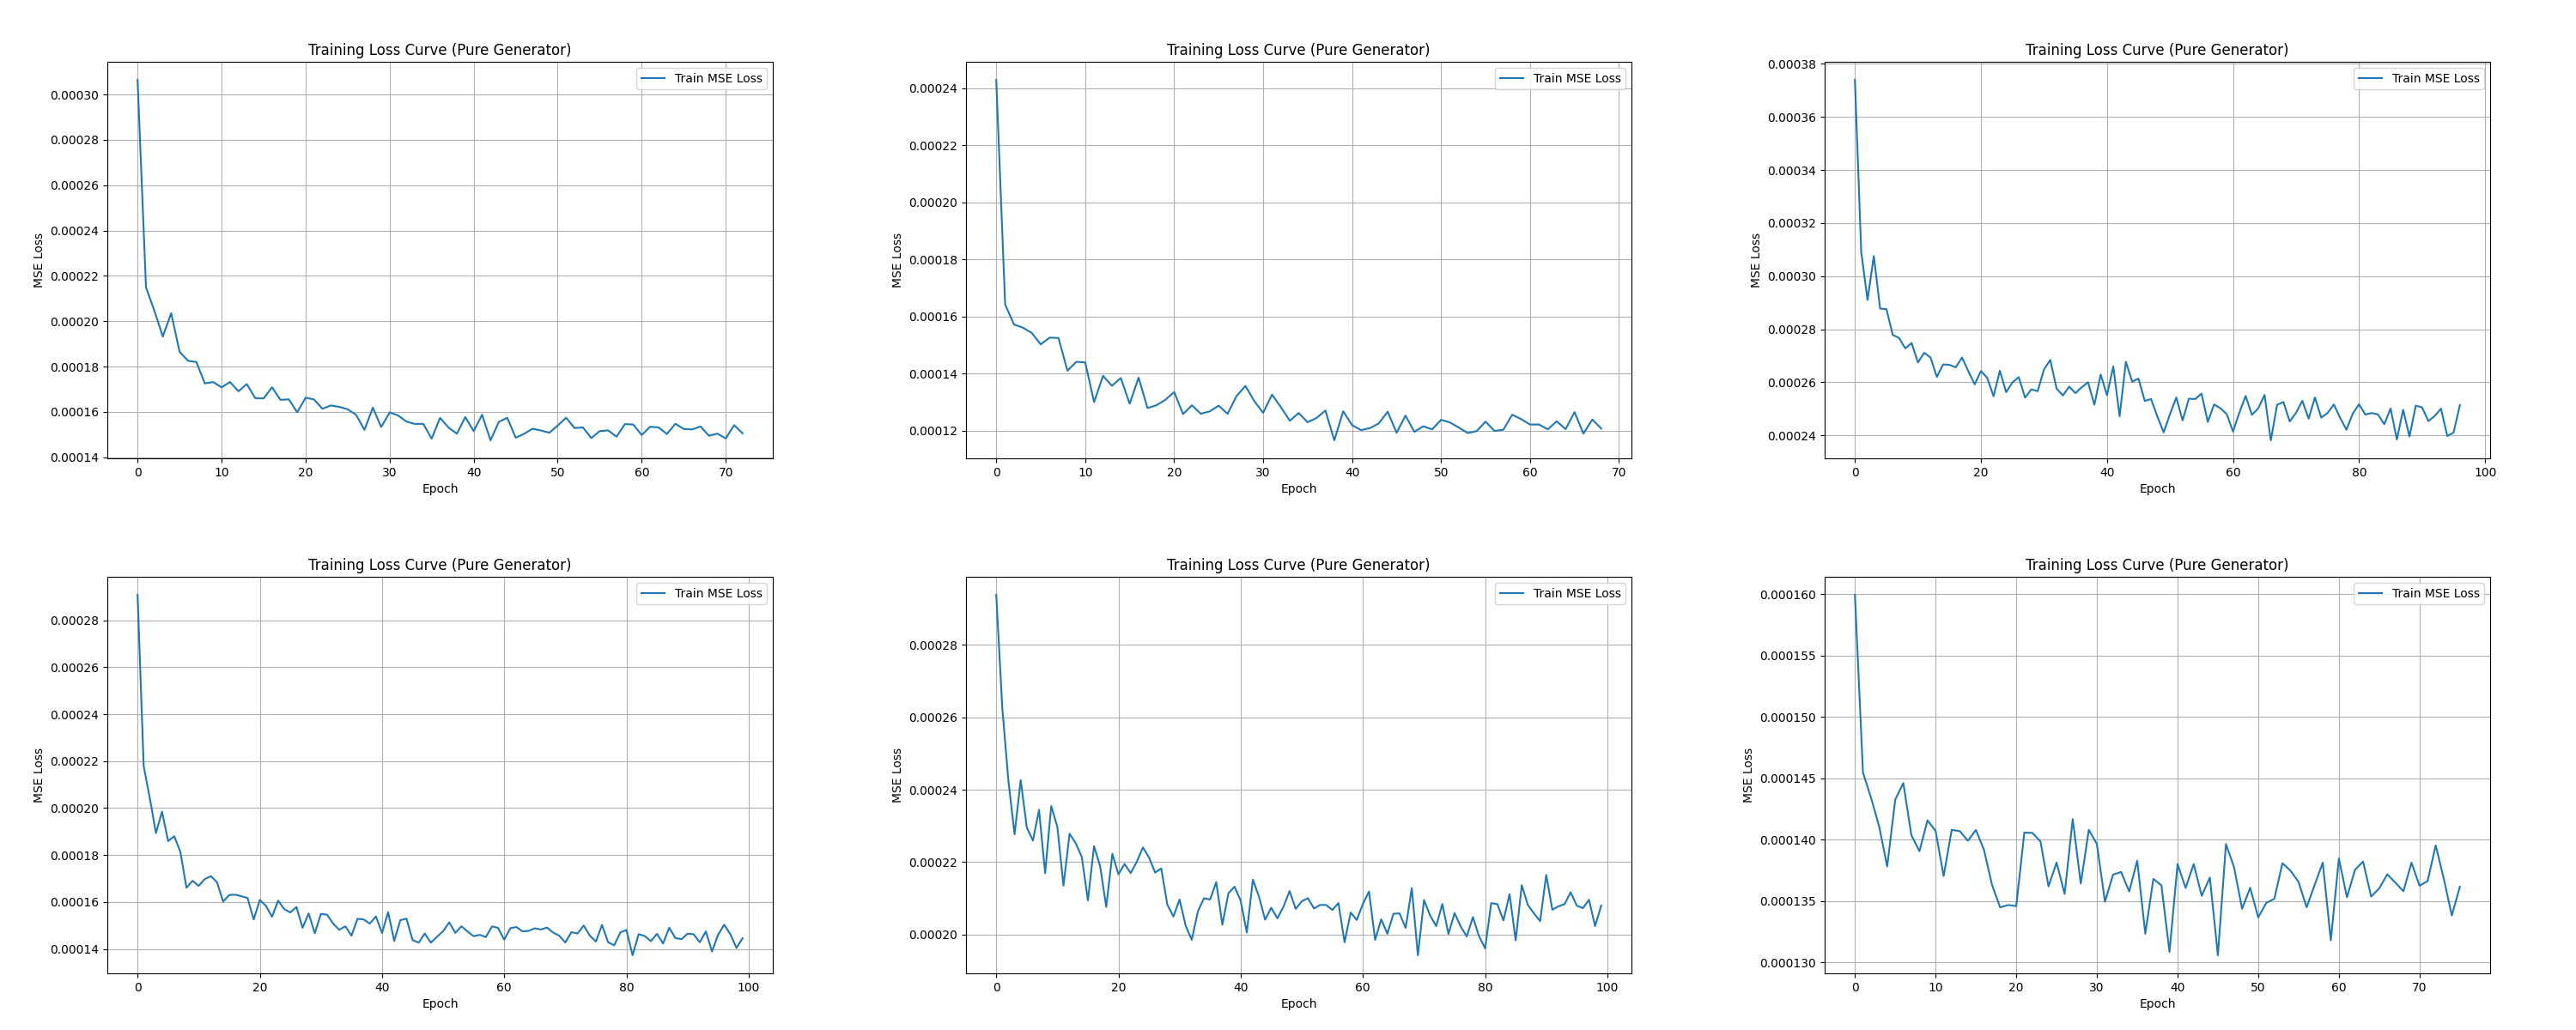
\includegraphics[width=0.8\textwidth]{figures/chap3/combined_LSTM_mse_loss_curve.png} 
    \caption{长短期记忆网络的均方误差训练损失图} % 图片下方的标题
    \label{LSTM的MSE训练损失图} % 【关键】设置引用标签，必须放在 \caption 之后！
\end{figure}

\begin{figure}[htbp] % [htbp] 是位置参数：这里(h)、页首(t)、页尾(b)、单独一页(p)
    \centering % 图片居中
    % width=\textwidth 表示图片宽度占满正文文本宽度
    % 如果在文件夹里，路径要是 figures/my_chart.png
    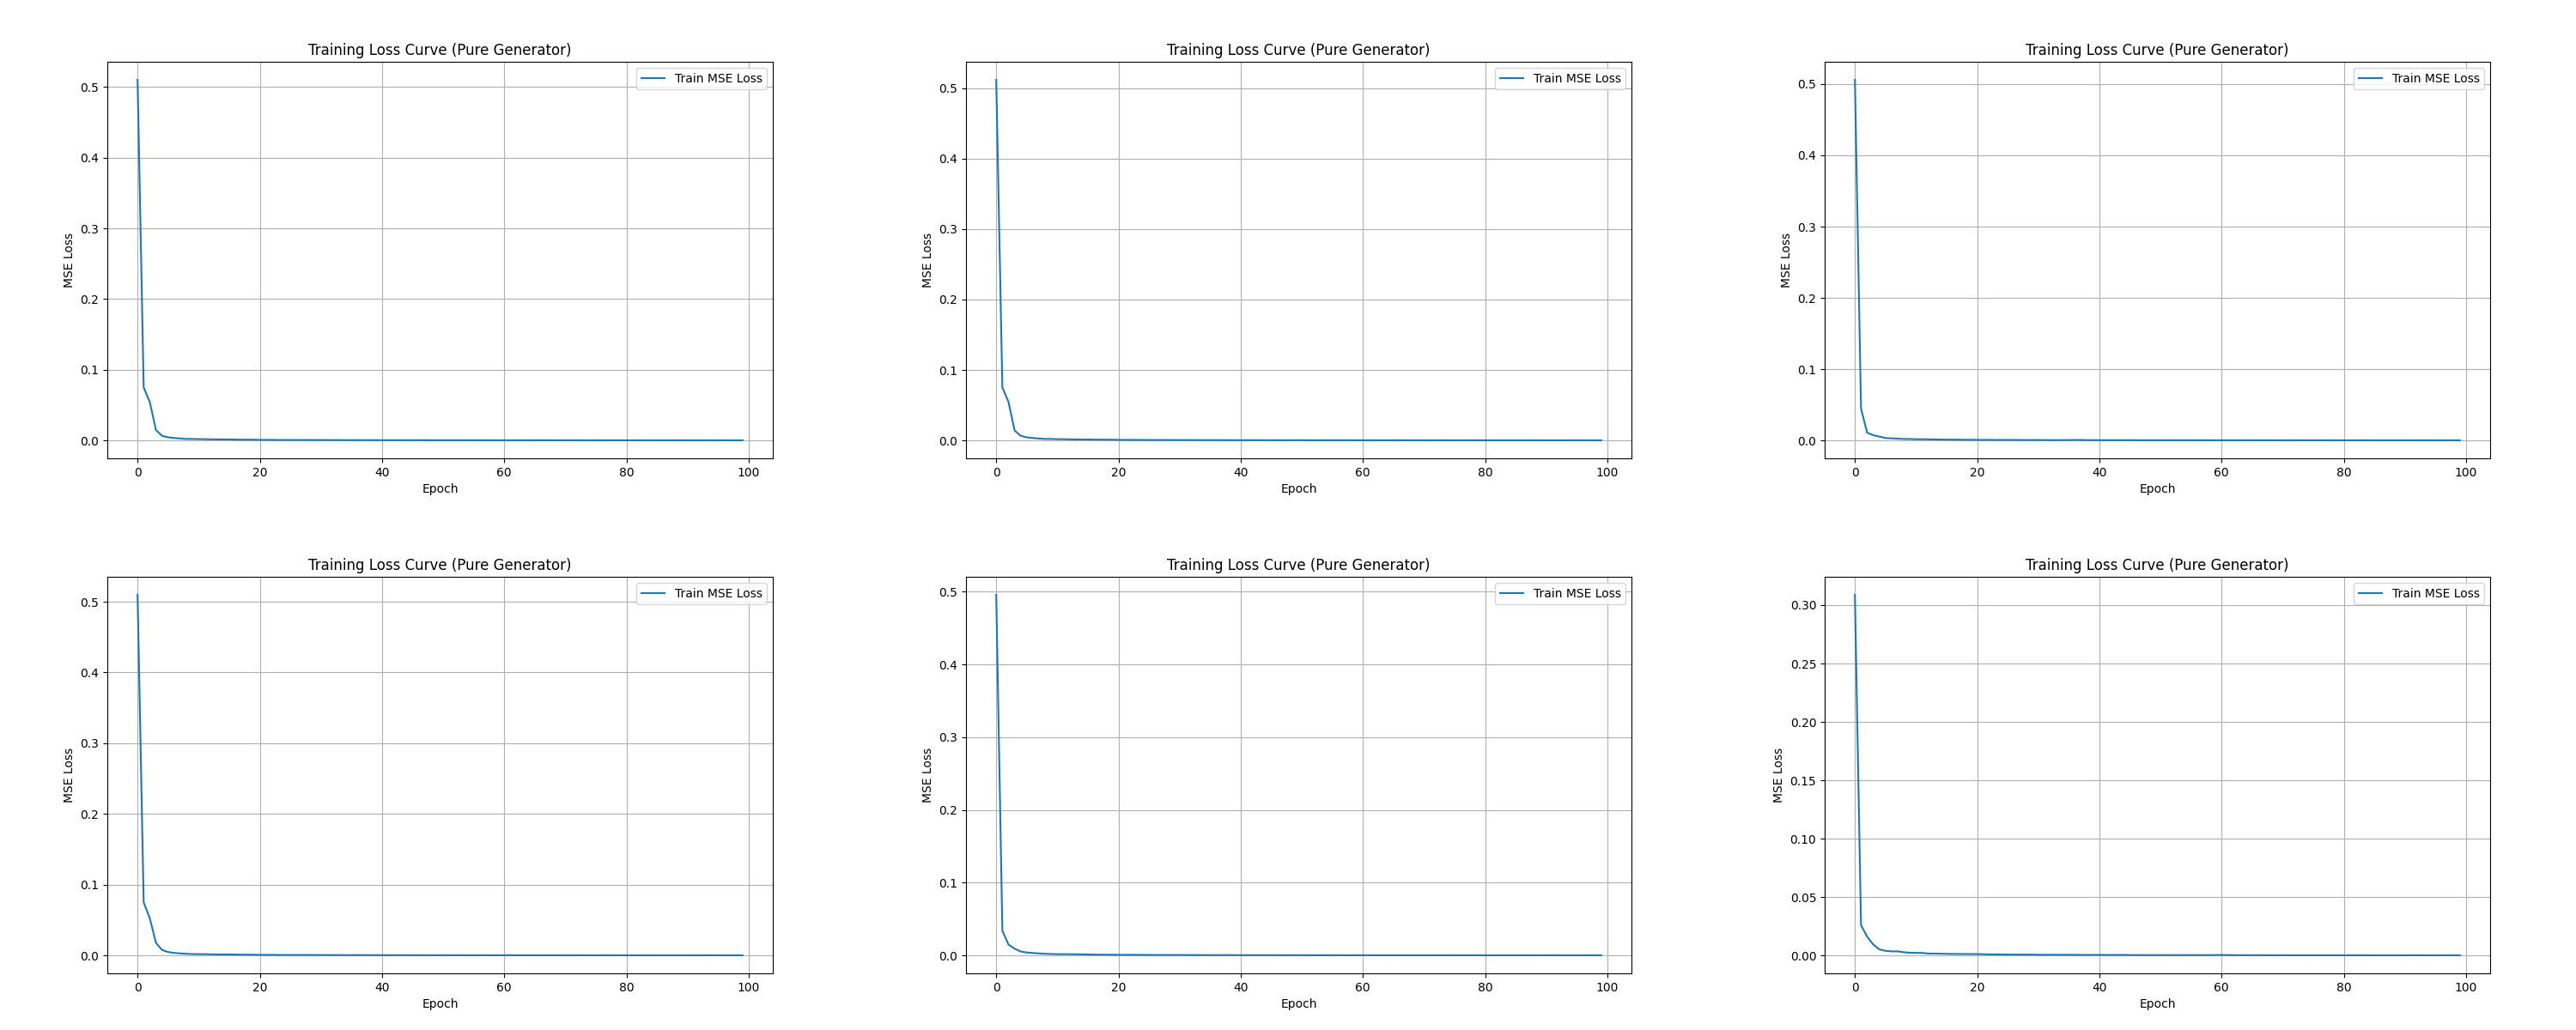
\includegraphics[width=0.8\textwidth]{figures/chap3/combined_Transformer_mse_loss_curve.png} 
    \caption{自注意力序列模型的均方误差训练损失图} % 图片下方的标题
    \label{Transformer的MSE训练损失图} % 【关键】设置引用标签，必须放在 \caption 之后！
\end{figure}

从图中可观察到明显的优化异构性：
循环神经网络（门控循环单元/长短期记忆网络）表现出早熟收敛，损失在前 10 个 Epoch 快速下降后迅速进入平台期，易过度依赖自回归特征并陷入局部最优，导致样本外对市场风格切换的适应能力较弱。
而基于对抗与注意力机制的模型（自注意力序列模型/GCA）则呈现渐进式探索，其中 GCA 损失下降平缓、微调阶段更长，有效抑制了过拟合，使模型在保证信号保真度的同时持续优化数据分布。

% \begin{enumerate}
%     \item 循环神经网络 (GRU/LSTM)：呈现出 “早熟收敛 (Premature Convergence)” 的特征。如图中第一、二列所示，RNN 类模型的损失在前 10 个 Epoch 内呈断崖式下跌，随后迅速进入平台期。这种极快的收敛往往暗示模型过度利用了时间序列的自回归特性，容易陷入局部极小值，这也解释了其在样本外测试中对市场风格转换的适应性较差。
%     \item 对抗与注意力机制 (Transformer/MGCA)：呈现出 “渐进式探索”的特征。MGCA 的损失曲线下滑斜率相对平缓，且在达到稳态前经历了更长时间的微调（Fine-tuning）。这表明MGCA有效地阻止了生成器对历史数据的过拟合，迫使其在保持信号物理保真度的同时，不断调整分布以通过判别器的统计检验。
% \end{enumerate}

尽管收敛路径各异，GCA 在六个组合上最终均收敛至与基准相当甚至更低的Loss水平（$10^{-4}$ 量级），表明该多目标优化系统有效实现了帕累托最优，未出现模式崩塌或梯度消失问题。


% \subsubsection{投资组合实证表现及分析}

表 \ref{tab:comparison_summary_full} 汇总了各模型在六个测试组合上的核心回测指标。实验结果显示，GCA 框架在多数场景下取得了较好的风险调整后收益（Sharpe Ratio）。
% \subsubsection{主要发现与归因分析}
基于表 \ref{tab:comparison_summary_full} 的结果，GCA在六类组合中总体呈现更稳定的风险调整后收益。其优势主要体现在三个方面：一是在P2、P3等趋势较清晰组合中能够保留进攻性；二是在P5高波动组合中降低基准模型失效风险；三是在P1、P4、P6等结构较复杂组合中保持较低换手率和较好的风险收益平衡。这些结果说明，GCA的核心贡献在于提升多资产投资组合管理中的信号稳定性、权重配置合理性与风险调整收益，而不是单纯依赖某一组合的收益表现。


% \begin{enumerate}[label=\arabic*.]
% \item \textbf{维度一：不同市场趋势的适应性}

% 这一维度验证模型是否仅在某些特定行情（如单边牛市）下有效，还是在各种市场环境下都能保持稳健。
% 牛市/高收益环境下的进攻能力：
% 在 P2（农产品） 和 P3（能源化工） 这种呈现明显上涨趋势的组合中，MGCA 取得了最高的累计收益率（分别为 110.50\% 和 39.42\%）。这说明在市场趋势明确时，MGCA 能够充分捕捉上涨红利，优于 Transformer 等基准模型。
% 震荡/复杂环境下的稳健性：
% 在 P1（宏观敏感） 和 P6（多元分散） 这种资产相关性复杂、宏观因子交织的场景下，MGCA 依然取得了最优的夏普比率（Sharpe Ratio）。这表明 MGCA 能够有效处理多维度的宏观噪音，提取有效信号。

% \item  \textbf{维度二：极端风险与高波动环境的防御性}

% 这是 多智能体群组交叉对抗框架表现最突出的维度，验证了其在应对市场剧烈波动或崩盘时的生存能力。
% 高波动与危机规避能力：
% P5（高波动） 是最关键的验证场景。在该组合中，基准模型（如 GRU）出现了严重的亏损（累计收益率 -68.18\%，夏普比率负值），而 MGCA 不仅实现了正向收益（47.27\%），还将最大回撤控制在 -20.83\%（远优于 GRU 的 -72.78\%）。
% 这证明了 多智能体群组交叉对抗框架具有极强的尾部风险感知能力，能够在市场极度不稳定时及时止损或切换防御策略，这是其相对于传统深度学习模型（LSTM/GRU）的核心优势。

% \item  \textbf{维度三：跨资产类别的泛化能力}

% 这一维度验证模型是否“过拟合”于某一类特定资产（如只懂股票不懂期货），还是在不同属性的资产上都能通用。
% 资产属性的广泛覆盖：
% 表格涵盖了大宗商品（P2 农产品、P3 能源）、金融属性强的资产（P4 避险对冲，通常包含黄金/国债等）以及混合资产（P6）。
% MGCA 在所有这些截然不同的资产类别中，夏普比率均稳定在 0.4 到 0.7 之间，且 consistently（一致地）优于其他模型。
% 低换手率带来的交易优势：
% 观察“平均换手”一列，MGCA 在绝大多数组合（P1, P2, P3, P4, P5）中的换手率都是最低的。这意味着 MGCA 不仅能适应不同资产，还能生成更平滑、噪音更少的交易信号，减少了不必要的摩擦成本，体现了其对资产底层逻辑的深刻理解而非简单的过拟合。
% \end{enumerate}


\begin{table}[H]
\centering
\caption{GCA 与基准模型在全部六个实验组合上的完整回测表现对比}
\label{tab:comparison_summary_full}
\footnotesize
\setlength{\tabcolsep}{1.5pt}
\renewcommand{\arraystretch}{1.15}
\begin{tabular}{@{}p{0.115\textwidth}p{0.145\textwidth}p{0.085\textwidth}p{0.085\textwidth}p{0.095\textwidth}p{0.095\textwidth}p{0.095\textwidth}p{0.070\textwidth}p{0.075\textwidth}@{}}
\toprule
\textbf{组合} & \textbf{模型} & \textbf{夏普比率} & \textbf{卡玛比率} & \textbf{累计收益率} & \textbf{年化波动率} & \textbf{最大回撤} & \textbf{胜率} & \textbf{平均换手} \\
\midrule
\multirow{4}{*}{\shortstack[l]{P1 宏观敏感}}
& 门控循环单元 & 0.279 & 0.143 & 17.86\% & 12.97\% & -25.36\% & 50.4\% & 0.050 \\
& 长短期记忆网络 & 0.225 & 0.122 & 14.03\% & 12.63\% & -23.41\% & 50.6\% & 0.038 \\
& 自注意力序列模型 & 0.384 & 0.286 & 24.67\% & 12.99\% & -17.51\% & 50.1\% & 0.055 \\
& \textbf{GCA} & \textbf{0.421} & \textbf{0.269} & \textbf{26.93\%} & 13.18\% & \textbf{-20.59\%} & \textbf{51.1\%} & \textbf{0.024} \\
\midrule
\multirow{4}{*}{\shortstack[l]{P2 农产品}}
& 门控循环单元 & 0.430 & 0.235 & 73.12\% & 10.16\% & -18.60\% & 50.1\% & 0.092 \\
& 长短期记忆网络 & 0.603 & 0.335 & 101.93\% & 10.09\% & -18.22\% & 50.3\% & 0.055 \\
& 自注意力序列模型 & 0.604 & 0.363 & 102.31\% & 10.11\% & -16.86\% & 50.6\% & 0.040 \\
& \textbf{GCA} & \textbf{0.657} & \textbf{0.402} & \textbf{110.50\%} & 10.10\% & \textbf{-16.50\%} & \textbf{50.9\%} & \textbf{0.039} \\
\midrule
\multirow{4}{*}{\shortstack[l]{P3 能源化工}}
& 门控循环单元 & 0.313 & 0.254 & 21.51\% & 13.93\% & -17.14\% & 49.1\% & 0.090 \\
& 长短期记忆网络 & 0.354 & 0.277 & 24.69\% & 14.15\% & -18.08\% & 48.7\% & 0.075 \\
& 自注意力序列模型 & 0.515 & 0.480 & 35.87\% & 14.13\% & -15.14\% & 49.2\% & 0.077 \\
& \textbf{GCA} & \textbf{0.581} & \textbf{0.609} & \textbf{39.42\%} & 13.99\% & \textbf{-13.35\%} & \textbf{49.7\%} & \textbf{0.033} \\
\bottomrule
\end{tabular}
\end{table}
\begin{table}[H]
\centering
{\small\textbf{续表}}\\[0.5em]
\footnotesize
\setlength{\tabcolsep}{1.5pt}
\renewcommand{\arraystretch}{1.15}
\begin{tabular}{@{}p{0.115\textwidth}p{0.145\textwidth}p{0.085\textwidth}p{0.085\textwidth}p{0.095\textwidth}p{0.095\textwidth}p{0.095\textwidth}p{0.070\textwidth}p{0.075\textwidth}@{}}
\toprule
\textbf{组合} & \textbf{模型} & \textbf{夏普比率} & \textbf{卡玛比率} & \textbf{累计收益率} & \textbf{年化波动率} & \textbf{最大回撤} & \textbf{胜率} & \textbf{平均换手} \\
\midrule
\multirow{4}{*}{\shortstack[l]{P4 避险对冲}}
& 门控循环单元 & 0.564 & 0.455 & 34.41\% & 22.46\% & -27.84\% & 48.8\% & 0.085 \\
& 长短期记忆网络 & 0.616 & 0.528 & 37.10\% & 22.18\% & -25.88\% & 48.9\% & 0.070 \\
& 自注意力序列模型 & 0.657 & 0.546 & 37.72\% & 21.17\% & -25.47\% & 48.5\% & 0.058 \\
& \textbf{GCA} & \textbf{0.692} & \textbf{0.628} & \textbf{39.48\%} & 21.65\% & \textbf{-23.85\%} & 48.2\% & \textbf{0.038} \\
\midrule
\multirow{4}{*}{\shortstack[l]{P5 高波动}}
& 门控循环单元 & -0.750 & -0.105 & -68.18\% & 10.23\% & -72.78\% & 47.4\% & 0.373 \\
& 长短期记忆网络 & 0.118 & 0.049 & 10.58\% & 10.05\% & -24.33\% & 49.4\% & 0.124 \\
& 自注意力序列模型 & 0.067 & 0.024 & 5.88\% & 9.85\% & -27.29\% & 49.5\% & 0.122 \\
& \textbf{GCA} & \textbf{0.543} & \textbf{0.258} & \textbf{47.27\%} & 9.88\% & \textbf{-20.83\%} & \textbf{51.1\%} & \textbf{0.035} \\
\midrule
\multirow{4}{*}{\shortstack[l]{P6 多元分散}}
& 门控循环单元 & 0.471 & 0.380 & 44.81\% & 13.56\% & -16.79\% & 51.9\% & 0.070 \\
& 长短期记忆网络 & 0.365 & 0.268 & 32.62\% & 12.74\% & -17.33\% & 51.6\% & 0.082 \\
& 自注意力序列模型 & 0.436 & 0.398 & 41.87\% & 13.67\% & -14.98\% & 52.0\% & 0.048 \\
& \textbf{GCA} & \textbf{0.562} & \textbf{0.571} & \textbf{52.84\%} & 13.55\% & \textbf{-13.34\%} & 51.6\% & 0.070 \\
\bottomrule
\end{tabular}
\end{table}


% \subsubsection{产业链传导与宏观对冲能力的验证}

从组合差异看，P3的能源化工组合验证了GCA对产业链时滞关系的捕捉能力，P4说明该架构在宏观对冲组合中能够改善盈亏结构，P5则体现了其在高波动环境下的防御性。P1和P2的结果进一步表明，GCA并非只在单一市场状态下有效，而是能够通过异构智能体的协同分工，在趋势、震荡和低相关资产池中维持较稳定的信号生成能力。

\noindent\textbf{辅助校验层的实证效果}\par

为观察辅助校验层对GCA输出权重的影响，本节在六组实验组合上比较GCA模型与接入量化相对强度指标过滤后的样本外回测表现。该实验不改变GCA主体结构，仅在模型输出后增加状态确认与权重过滤。表 \ref{tab:qr_gca_results} 汇总了对比结果。

\begin{table}[H]
\centering
\caption{GCA 与辅助校验层在六类组合上的回测对比}
\label{tab:qr_gca_results}
\footnotesize
\setlength{\tabcolsep}{2pt}
\renewcommand{\arraystretch}{1.15}
\begin{tabular}{@{}p{0.15\textwidth}p{0.18\textwidth}p{0.085\textwidth}p{0.095\textwidth}p{0.095\textwidth}p{0.095\textwidth}p{0.075\textwidth}p{0.085\textwidth}@{}}
\toprule
\textbf{组合} & \textbf{方法} & \textbf{夏普比率} & \textbf{累计收益率} & \textbf{年化收益率} & \textbf{最大回撤} & \textbf{胜率} & \textbf{$\Delta$ Sharpe} \\
\midrule
\multirow{2}{*}{\shortstack[l]{P1 宏观敏感\\(Gold,Oil,Cu,M)}}
& GCA & 0.4193 & 26.91\% & 5.54\% & -20.44\% & 50.78\% & --- \\
& \textbf{GCA+辅助校验层} & \textbf{1.6082} & \textbf{199.09\%} & \textbf{41.02\%} & -21.91\% & 52.25\% & \textbf{+1.1889} \\
\midrule
\multirow{2}{*}{\shortstack[l]{P2 农产品\\(Corn,M,SR,CF)}}
& GCA & 0.6687 & 112.49\% & 6.76\% & -16.63\% & 50.88\% & --- \\
& \textbf{GCA+辅助校验层} & \textbf{1.0208} & \textbf{193.29\%} & \textbf{11.61\%} & -16.63\% & 48.71\% & \textbf{+0.3521} \\
\bottomrule
\end{tabular}
\end{table}
\begin{table}[H]
\centering
{\small\textbf{续表}}\\[0.5em]
\footnotesize
\setlength{\tabcolsep}{2pt}
\renewcommand{\arraystretch}{1.15}
\begin{tabular}{@{}p{0.15\textwidth}p{0.18\textwidth}p{0.085\textwidth}p{0.095\textwidth}p{0.095\textwidth}p{0.095\textwidth}p{0.075\textwidth}p{0.085\textwidth}@{}}
\toprule
\textbf{组合} & \textbf{方法} & \textbf{夏普比率} & \textbf{累计收益率} & \textbf{年化收益率} & \textbf{最大回撤} & \textbf{胜率} & \textbf{$\Delta$ Sharpe} \\
\midrule
\multirow{2}{*}{\shortstack[l]{P3 能源化工\\(Oil,MA,PP,TA)}}
& GCA & 0.4936 & 42.91\% & 4.88\% & -20.08\% & 51.31\% & --- \\
& \textbf{GCA+辅助校验层} & \textbf{1.1148} & \textbf{141.43\%} & \textbf{16.07\%} & -32.17\% & 49.37\% & \textbf{+0.6212} \\
\midrule
\multirow{2}{*}{\shortstack[l]{P4 避险对冲\\(Au,Cu,Oil,ZC)}}
& GCA & 0.7077 & 40.57\% & 15.4\% & -24.25\% & 48.04\% & --- \\
& GCA+辅助校验层 & 0.4086 & 30.58\% & 11.61\% & -34.58\% & 45.63\% & -0.2991 \\
\bottomrule
\end{tabular}
\end{table}
\begin{table}[H]
\centering
{\small\textbf{续表}}\\[0.5em]
\footnotesize
\setlength{\tabcolsep}{2pt}
\renewcommand{\arraystretch}{1.15}
\begin{tabular}{@{}p{0.15\textwidth}p{0.18\textwidth}p{0.085\textwidth}p{0.095\textwidth}p{0.095\textwidth}p{0.095\textwidth}p{0.075\textwidth}p{0.085\textwidth}@{}}
\toprule
\textbf{组合} & \textbf{方法} & \textbf{夏普比率} & \textbf{累计收益率} & \textbf{年化收益率} & \textbf{最大回撤} & \textbf{胜率} & \textbf{$\Delta$ Sharpe} \\
\midrule
\multirow{2}{*}{\shortstack[l]{P5 高波动\\(V,MA,TA,PP)}}
& GCA & 0.4819 & 41.87\% & 4.76\% & -20.64\% & 51.35\% & --- \\
& \textbf{GCA+辅助校验层} & \textbf{1.1235} & \textbf{142.01\%} & \textbf{16.13\%} & -34.88\% & 49.91\% & \textbf{+0.6416} \\
\midrule
\multirow{2}{*}{\shortstack[l]{P6 多元分散\\(Au,CF,I,SR,ZC)}}
& GCA & 0.5723 & 53.16\% & 7.66\% & -12.94\% & 51.6\% & --- \\
& \textbf{GCA+辅助校验层} & \textbf{0.8214} & \textbf{111.35\%} & \textbf{16.05\%} & -14.33\% & 50.23\% & \textbf{+0.2491} \\
\bottomrule
\end{tabular}
\end{table}


\begin{figure}[htbp]
    \centering
    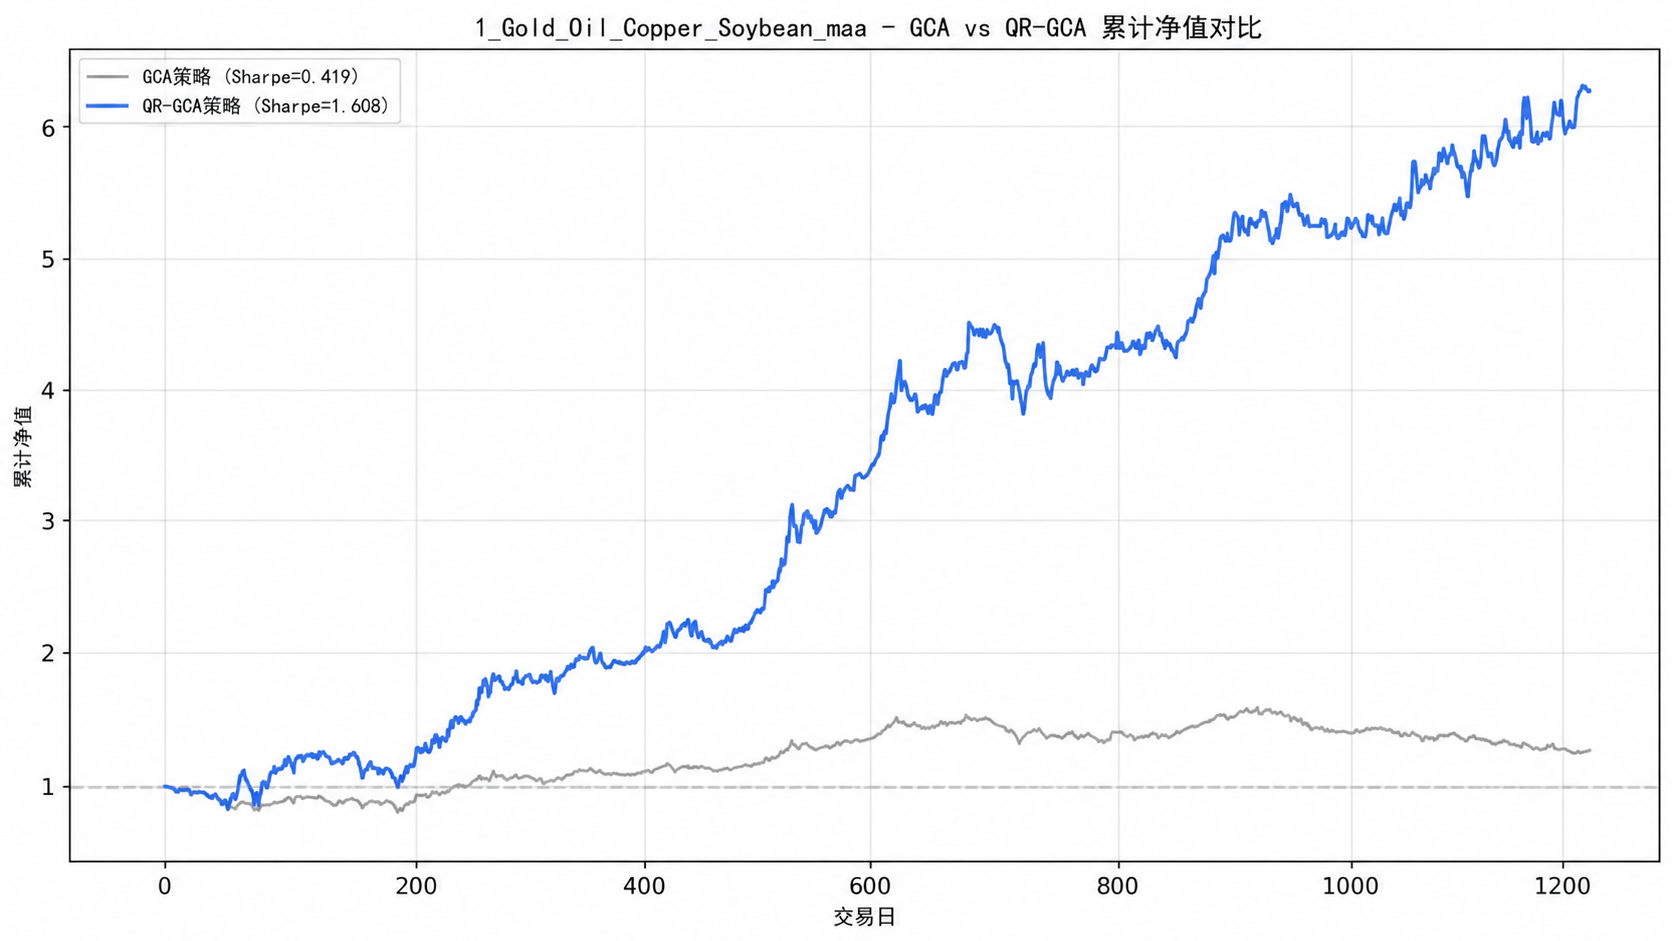
\includegraphics[width=0.48\textwidth]{figures/chap3/qr_gca/P1_comparison.png}
    \hfill
    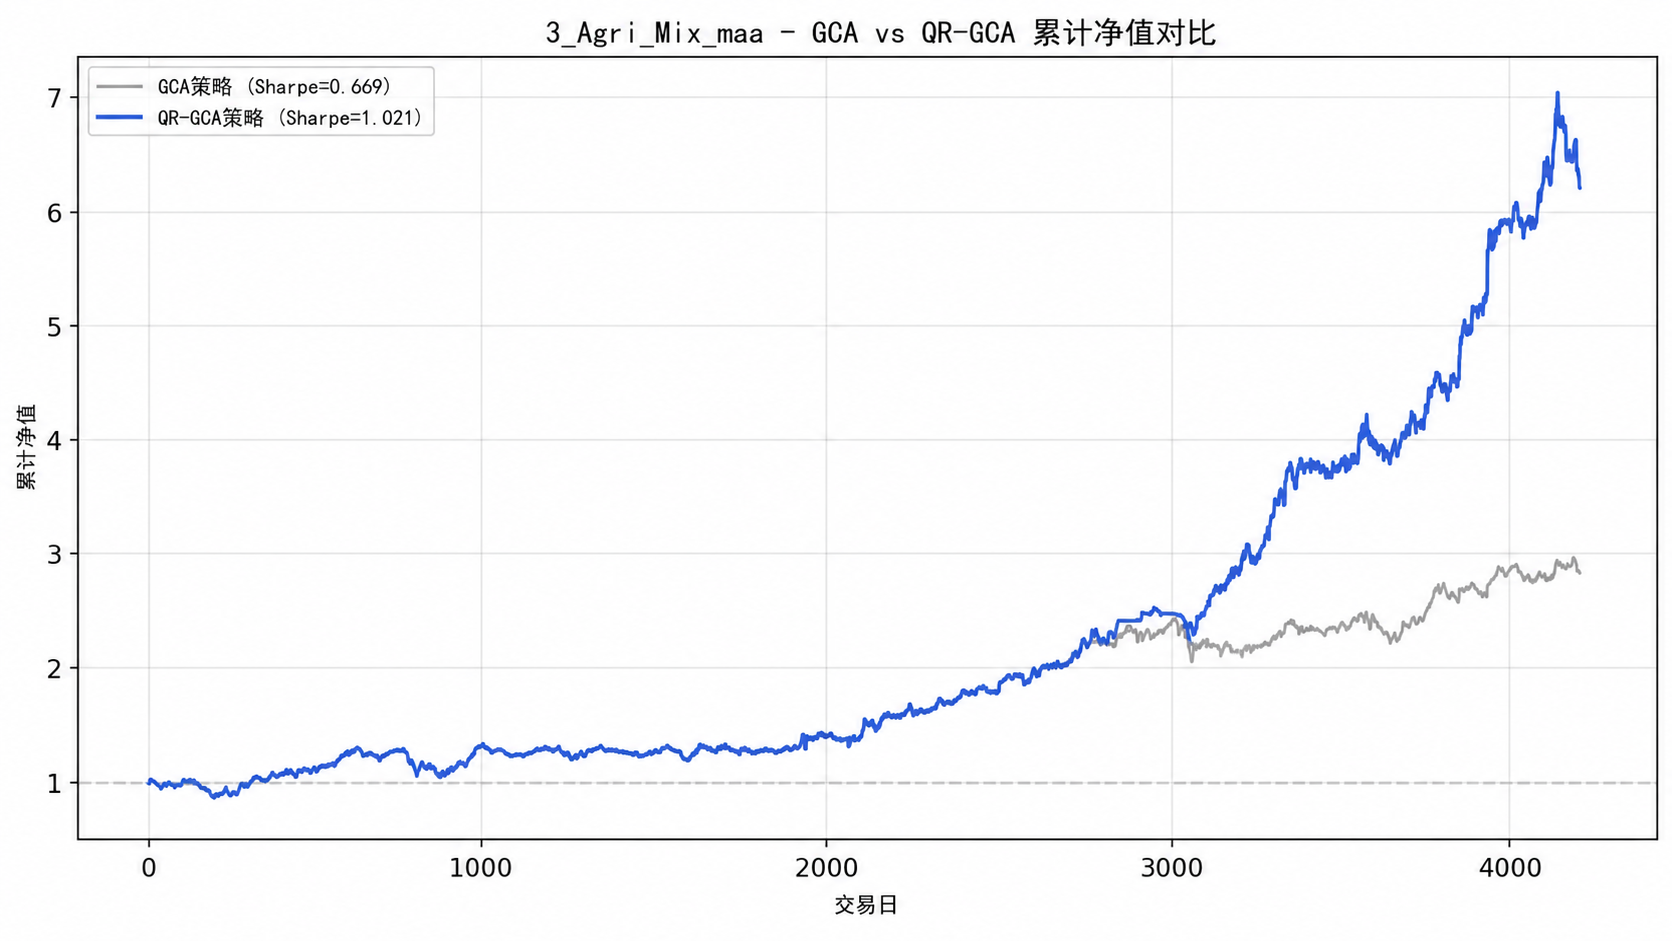
\includegraphics[width=0.48\textwidth]{figures/chap3/qr_gca/P2_comparison.png}
    \\[0.5em]
    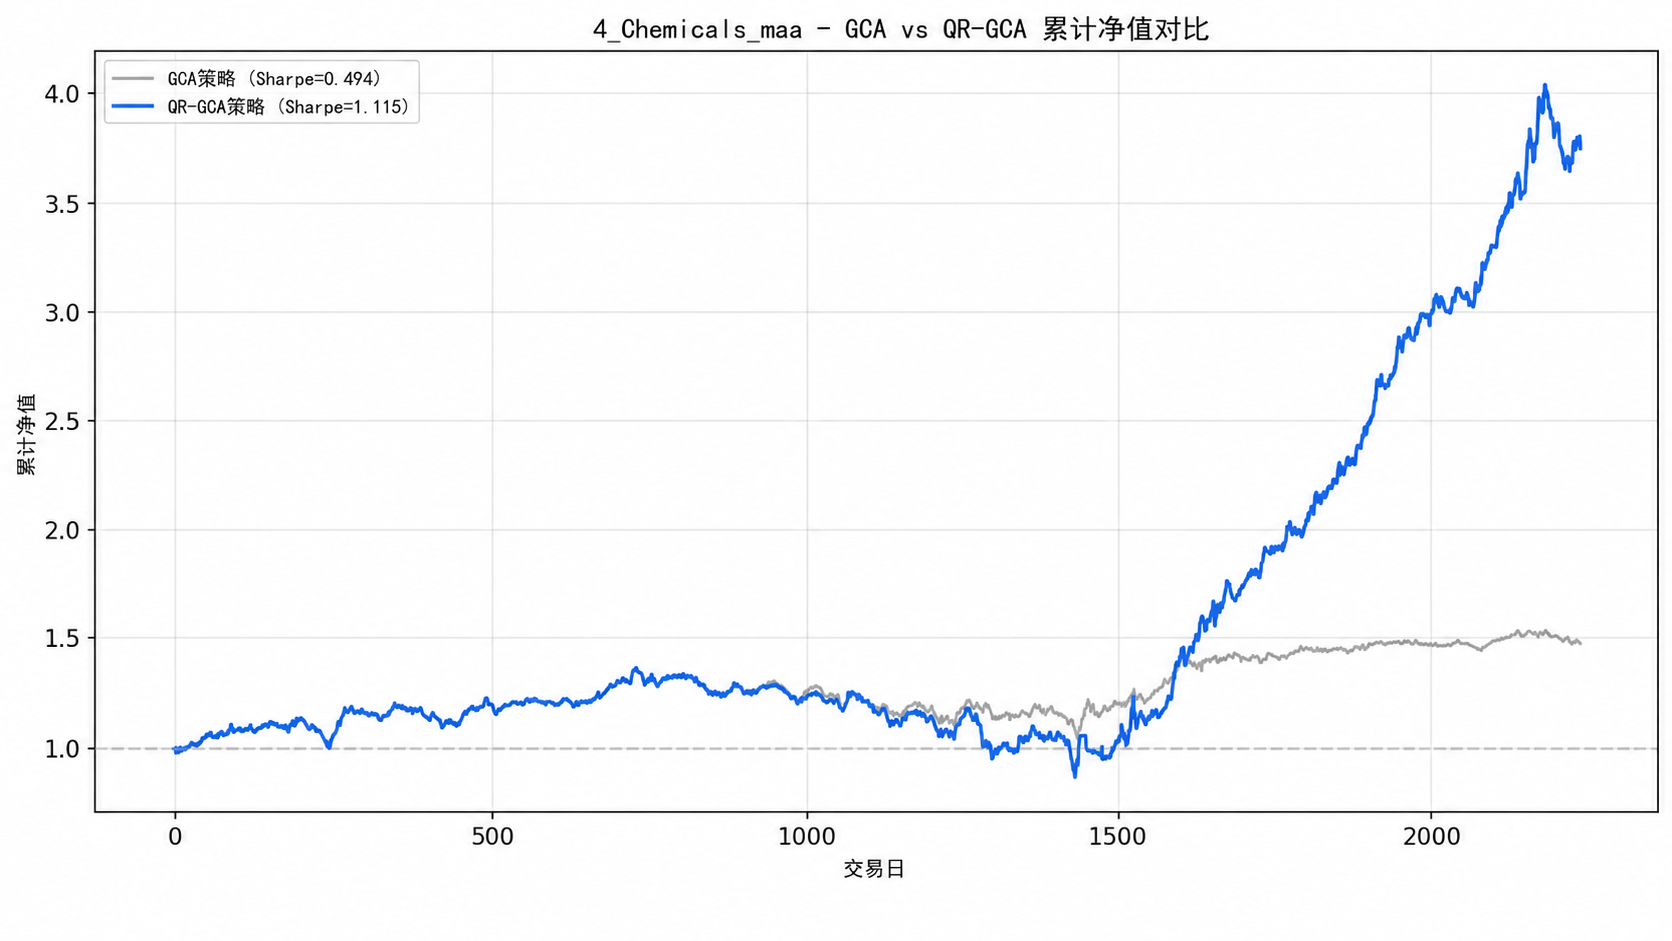
\includegraphics[width=0.48\textwidth]{figures/chap3/qr_gca/P3_comparison.png}
    \hfill
    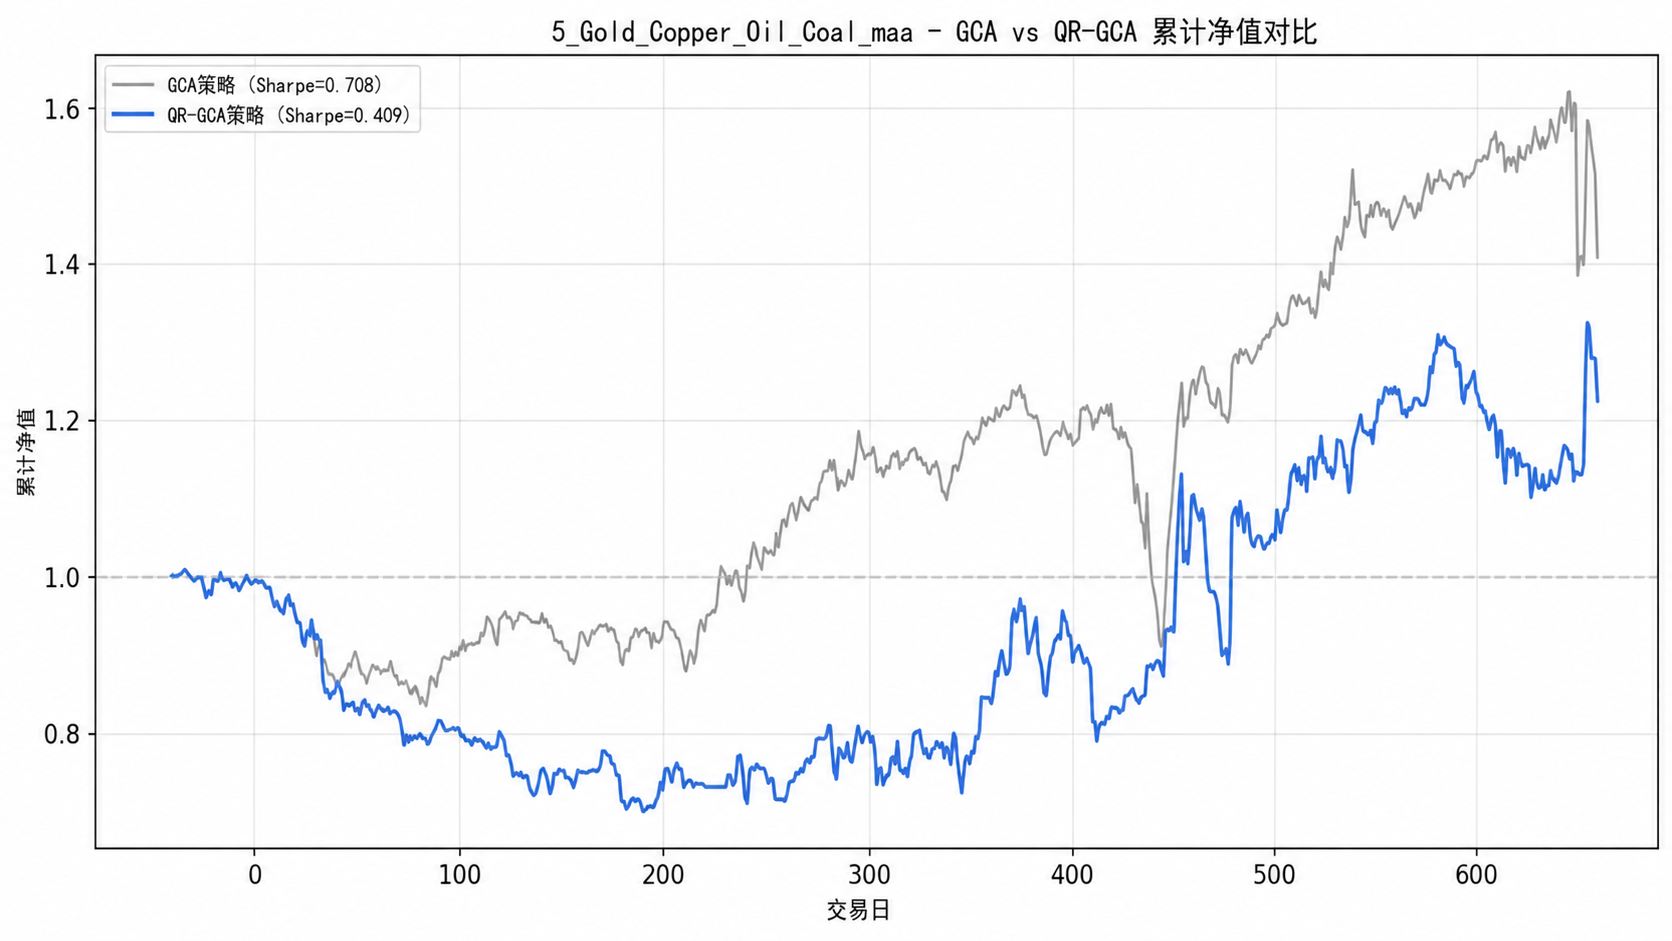
\includegraphics[width=0.48\textwidth]{figures/chap3/qr_gca/P4_comparison.png}
    \\[0.5em]
    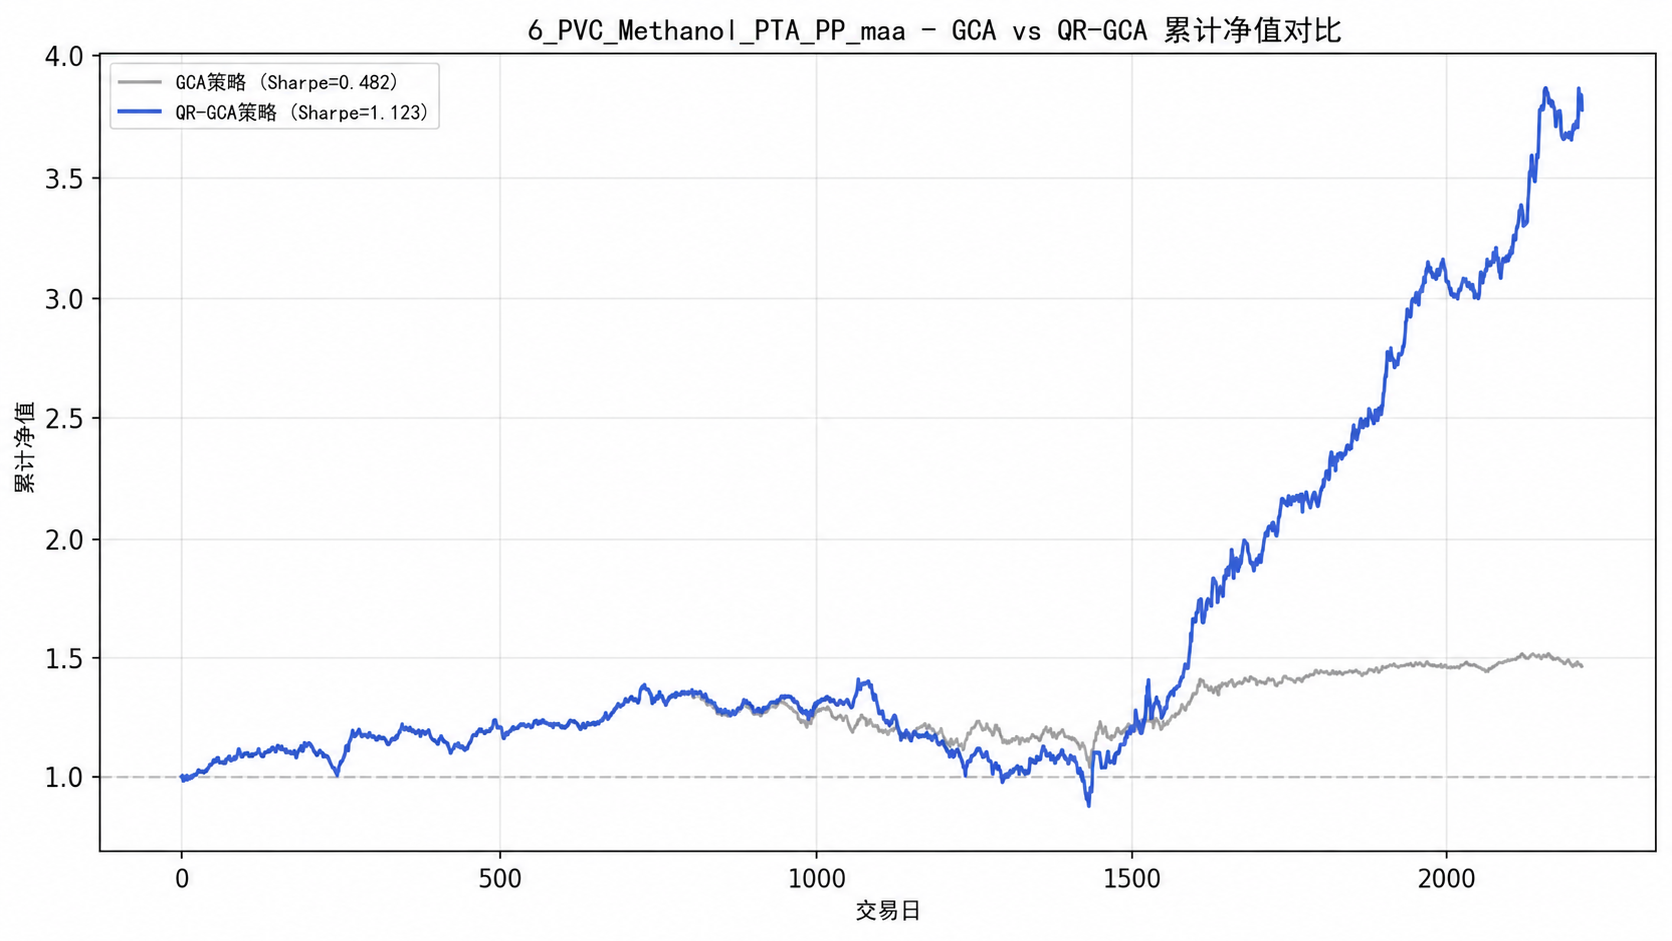
\includegraphics[width=0.48\textwidth]{figures/chap3/qr_gca/P5_comparison.png}
    \hfill
    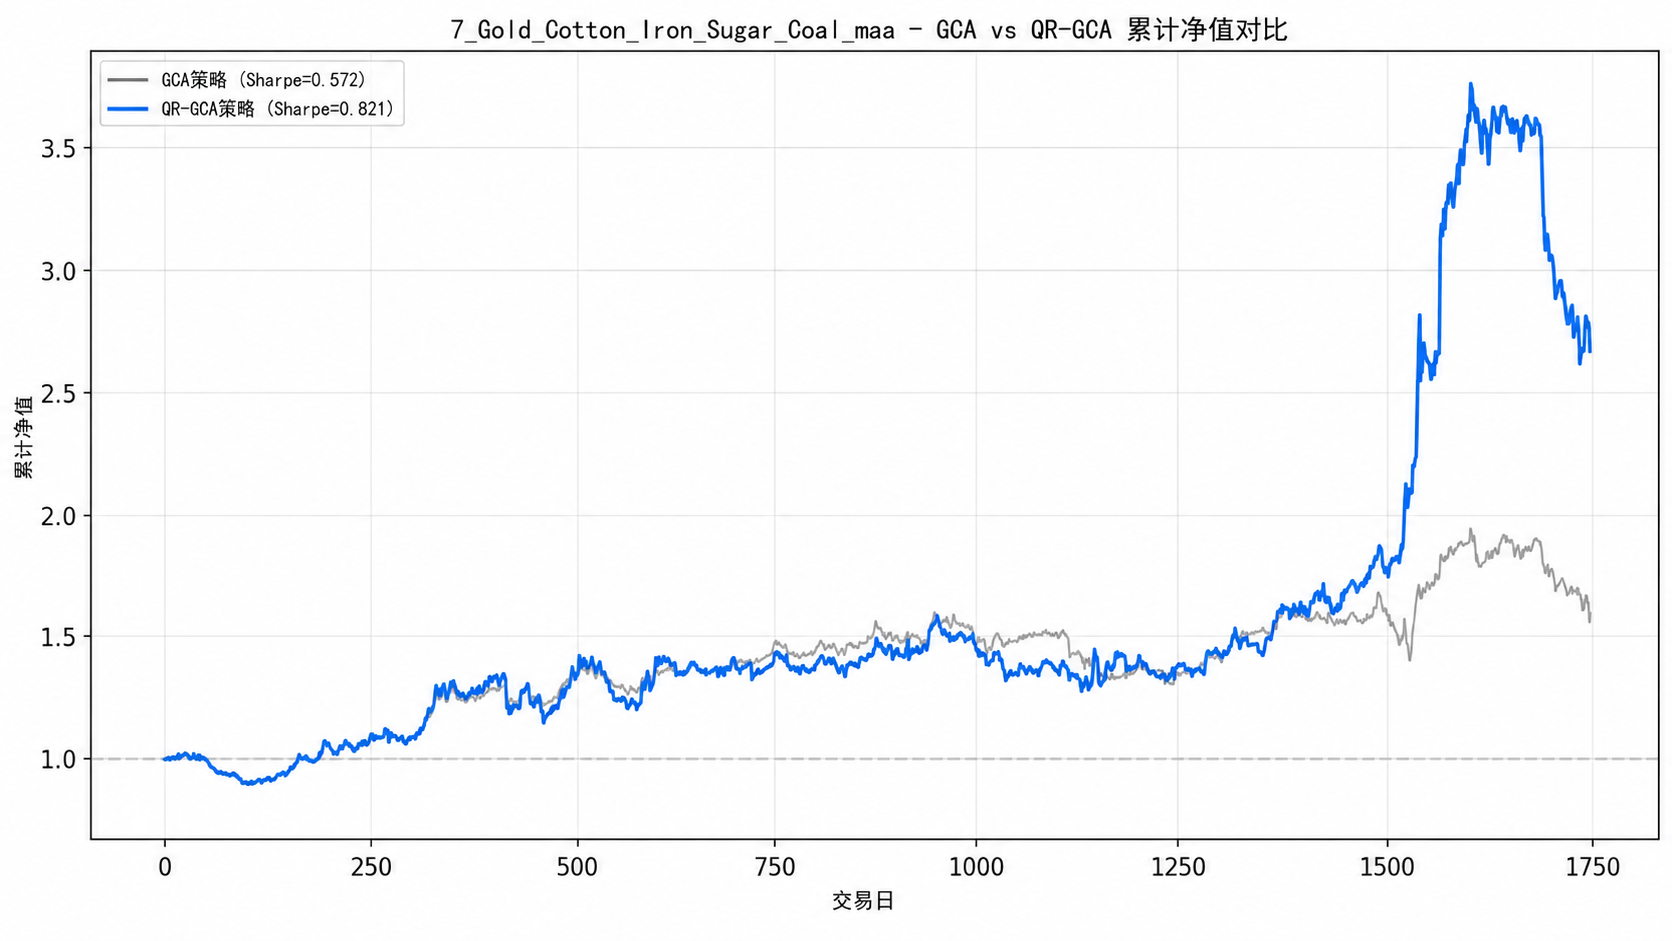
\includegraphics[width=0.48\textwidth]{figures/chap3/qr_gca/P6_comparison.png}
    \caption{GCA 与辅助校验层累计净值对比}
    \label{fig:qr_gca_comparison}
\end{figure}

% \subsubsection{辅助校验的系统性提升分析}

表 \ref{tab:qr_gca_results} 与图 \ref{fig:qr_gca_comparison} 显示，辅助校验层在多数趋势性组合中改善了GCA输出的交易可用性。P1、P2、P3、P5和P6的夏普比率均有提升，说明相对强弱确认在趋势性较强的组合中具有一定过滤价值。P4表现下降则表明，当组合收益主要来自跨资产对冲而非单向趋势时，统一市场状态过滤可能压制有效仓位。因此，该模块应被理解为GCA输出后的校验层，而不是本章的主要方法贡献。

\begin{figure}[htbp]
    \centering
    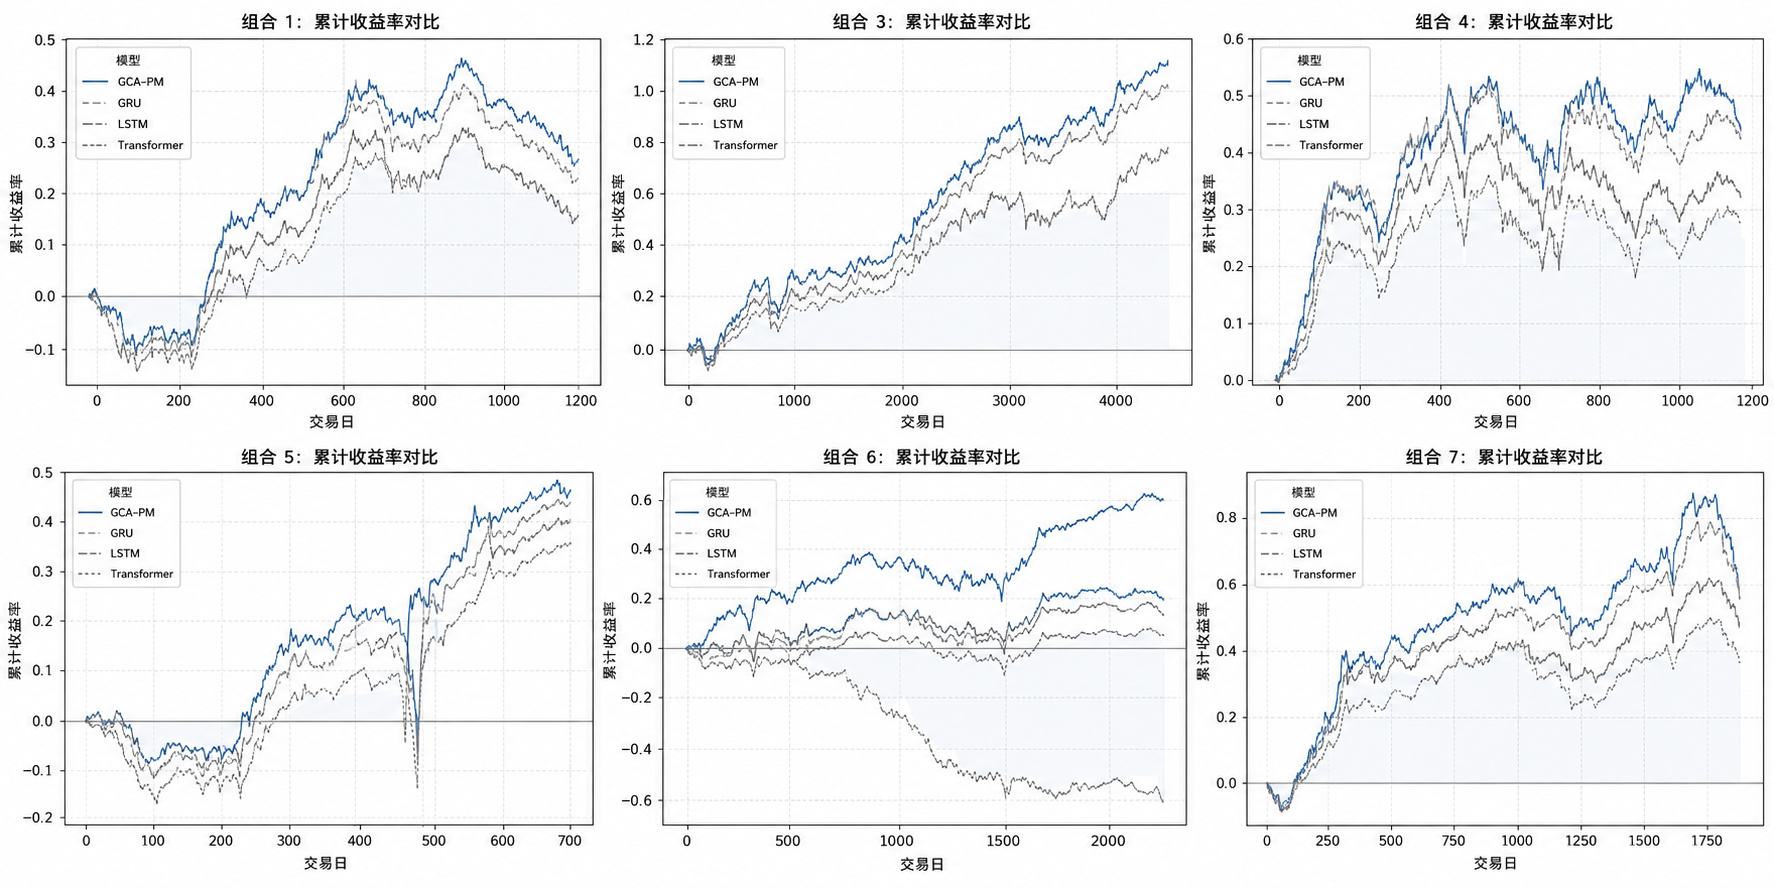
\includegraphics[width=0.95\textwidth]{figures/chap3/combined_累计收益率对比.jpg} 
    \caption{GCA 与基准模型累计净值对比}
    \label{fig:cumulative_returns}
\end{figure}

% \subsubsection{风险收益特征可视化}

% 图 \ref{fig:sharpe_ratio} 和 图 \ref{fig:max_drawdown} 直观呈现了各模型在风险调整后收益上的差距。
% 在 P4（避险对冲）组合中，MGCA 的柱状图高度（Sharpe 0.692）显著超越了表现第二的 Transformer（0.657）。更重要的是，这种提升并非来自于承担更大风险——如图 \ref{fig:max_drawdown} 所示，MGCA 的最大回撤（-23.85\%）同时也是所有模型中最低的。这意味着 MGCA 实现了投资组合在有效前沿上的 Pareto 改进，展现出夏普比率的帕累托改进。
% 在 P5 组合中，GRU 的回撤柱状图长达 -72\%（甚至超出了图表边界），而MGCA 被严格控制在 -21\% 以内，展现出尾部风险的截断。这验证了 $\mathcal{L}_{SR}$ 损失函数中分母项的惩罚机制，有效切断了高波动预测的梯度传播。


% \begin{figure}[htbp]
%     \centering
%     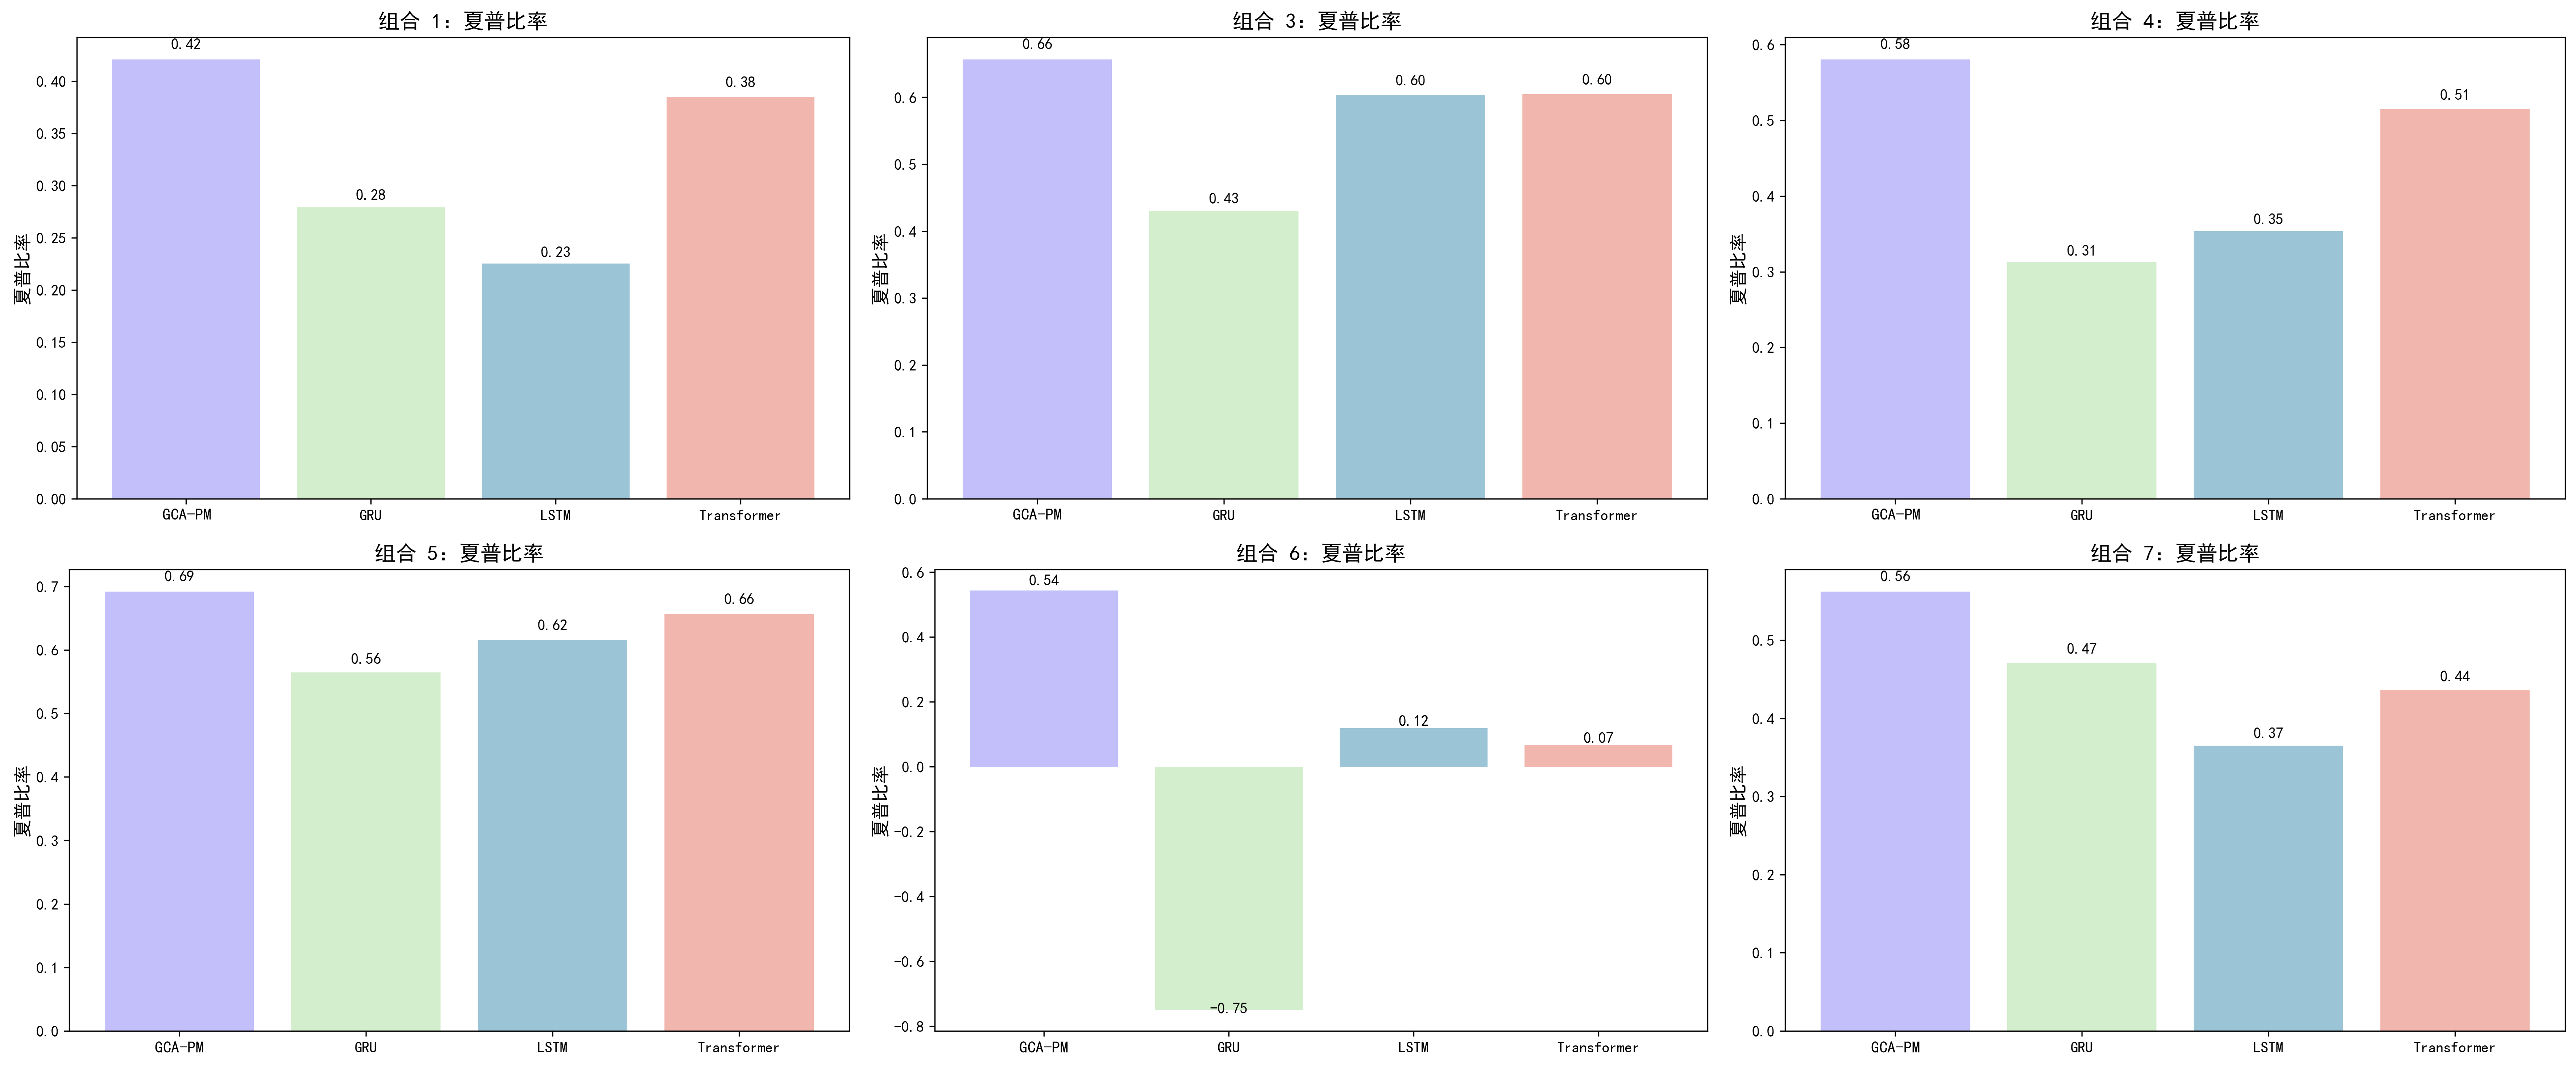
\includegraphics[width=0.95\textwidth]{figures/chap3/combined_夏普比率.jpg} 
%     \caption{各模型在不同资产组合下的夏普比率对比。MGCA 显示出系统性的风险调整后优势。}
%     \label{fig:sharpe_ratio}
% \end{figure}

% \begin{figure}[htbp]
%     \centering
%     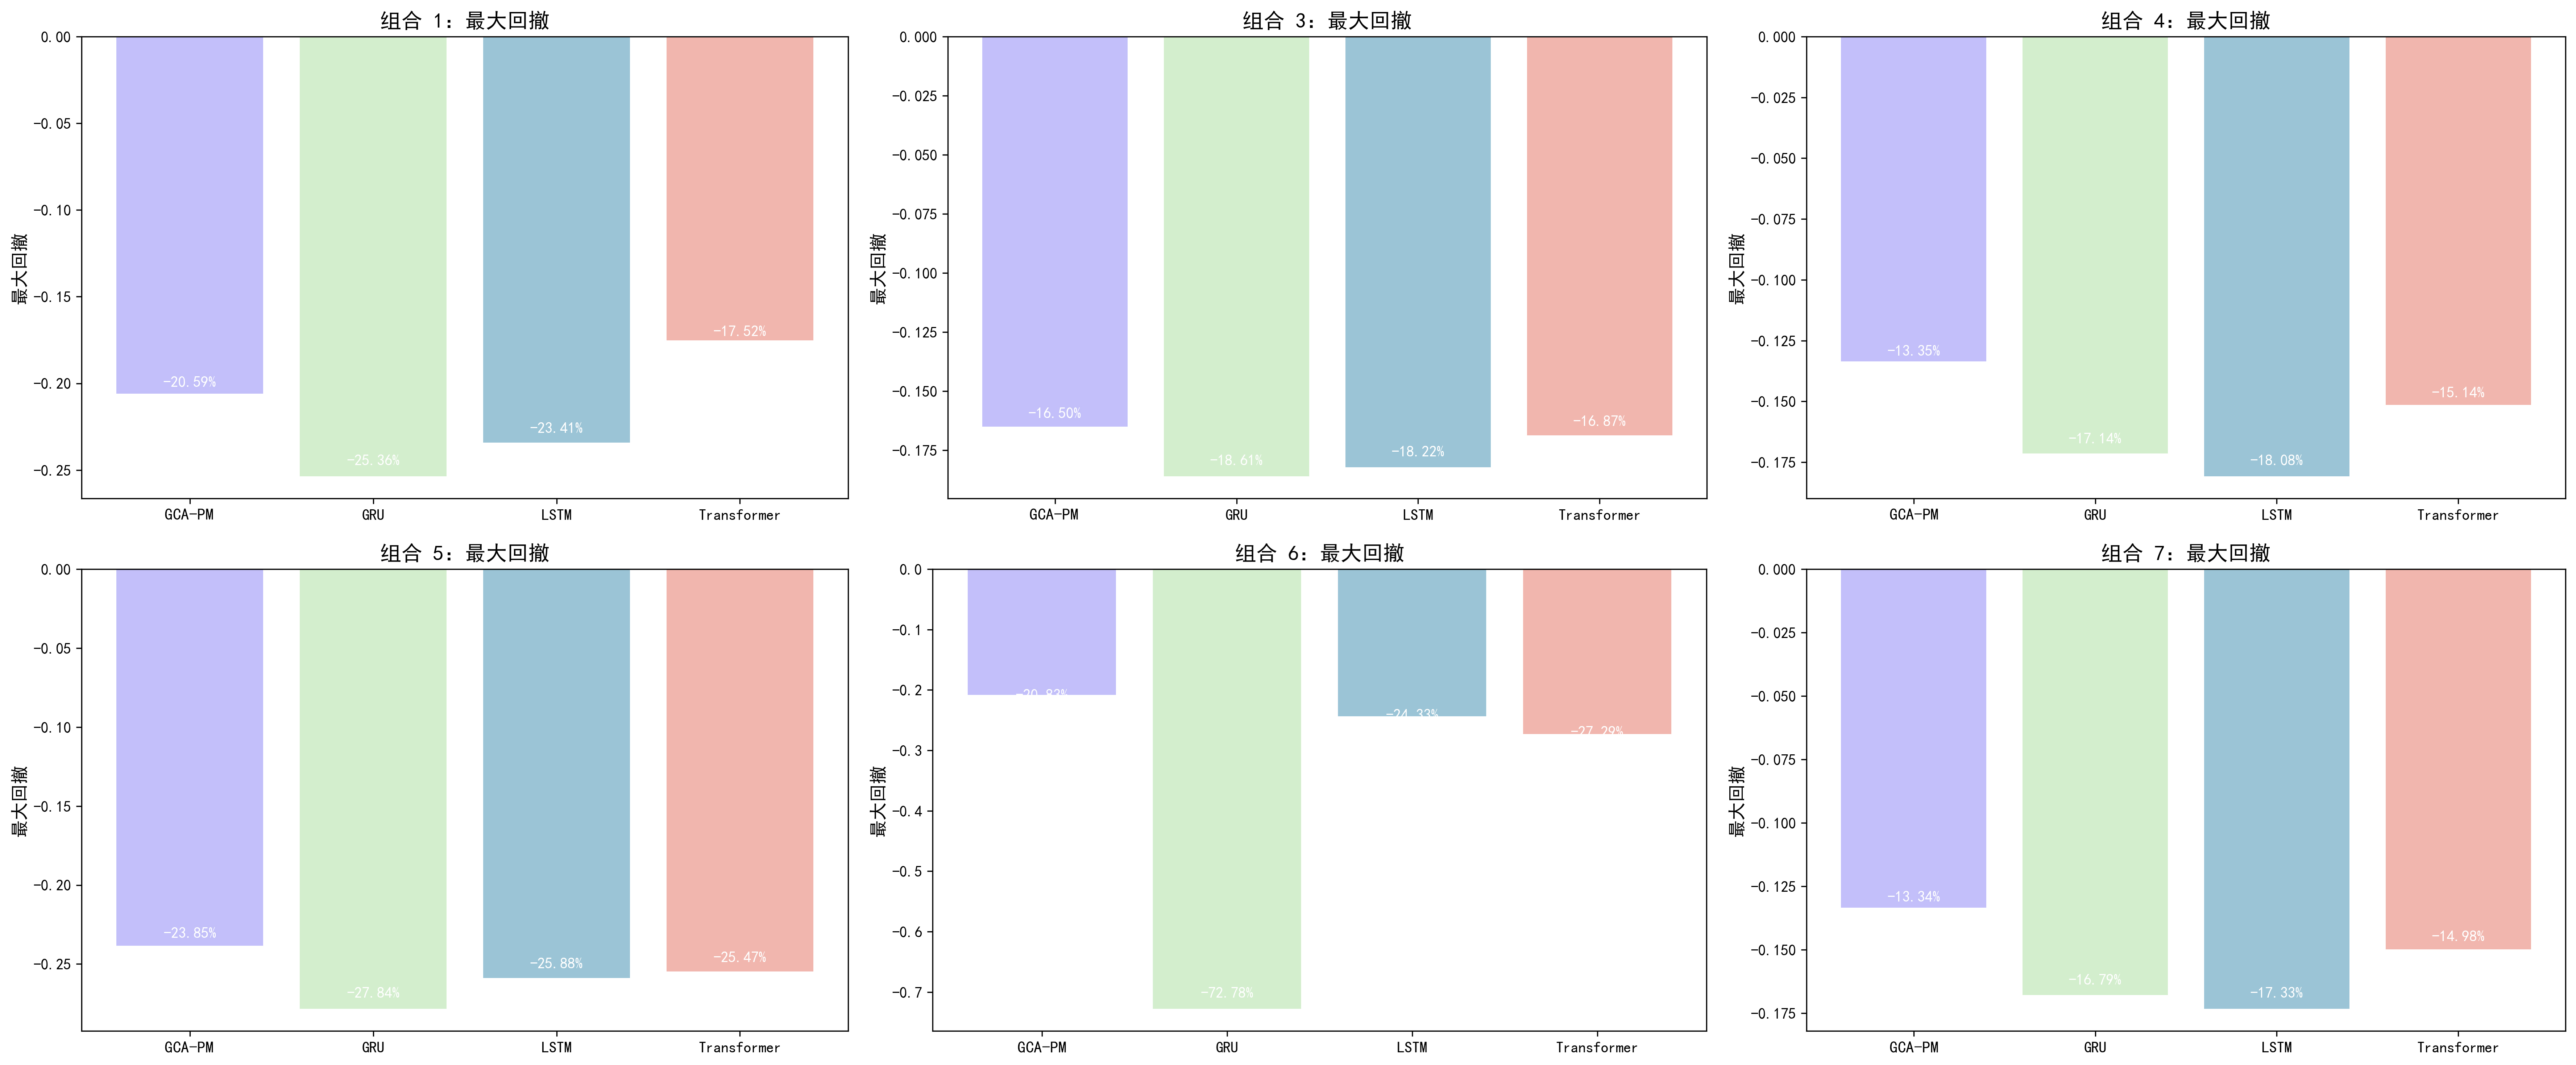
\includegraphics[width=0.95\textwidth]{figures/chap3/combined_最大回撤.jpg} 
%     \caption{各模型在不同资产组合下的最大回撤对比（数值越接近 0 表示风险控制越好）。}
%     \label{fig:max_drawdown}
% \end{figure}

% \subsubsection{多智能体协作机制的可解释性}
从多智能体协作机制看，图 \ref{fig:heatmap} 展示了元权重网络在不同市场状态下对门控循环单元、长短期记忆网络和自注意力序列模型的动态分配。低波动阶段，系统更依赖擅长均值回归的循环结构；趋势或高波动阶段，注意力结构权重上升。权重变化呈渐进式过渡，说明GCA机制能够在保持多样性的同时避免频繁切换。


% \begin{figure}[htbp]
%     \centering
%     \includegraphics[width=0.95\textwidth]
%     {figures/chap3/combined_权重历史热力图.jpg} 
%     \caption{GCA 子智能体权重动态演化热力图}
%     \label{fig:heatmap}
% \end{figure}


\begin{figure}[htbp]
    \centering
    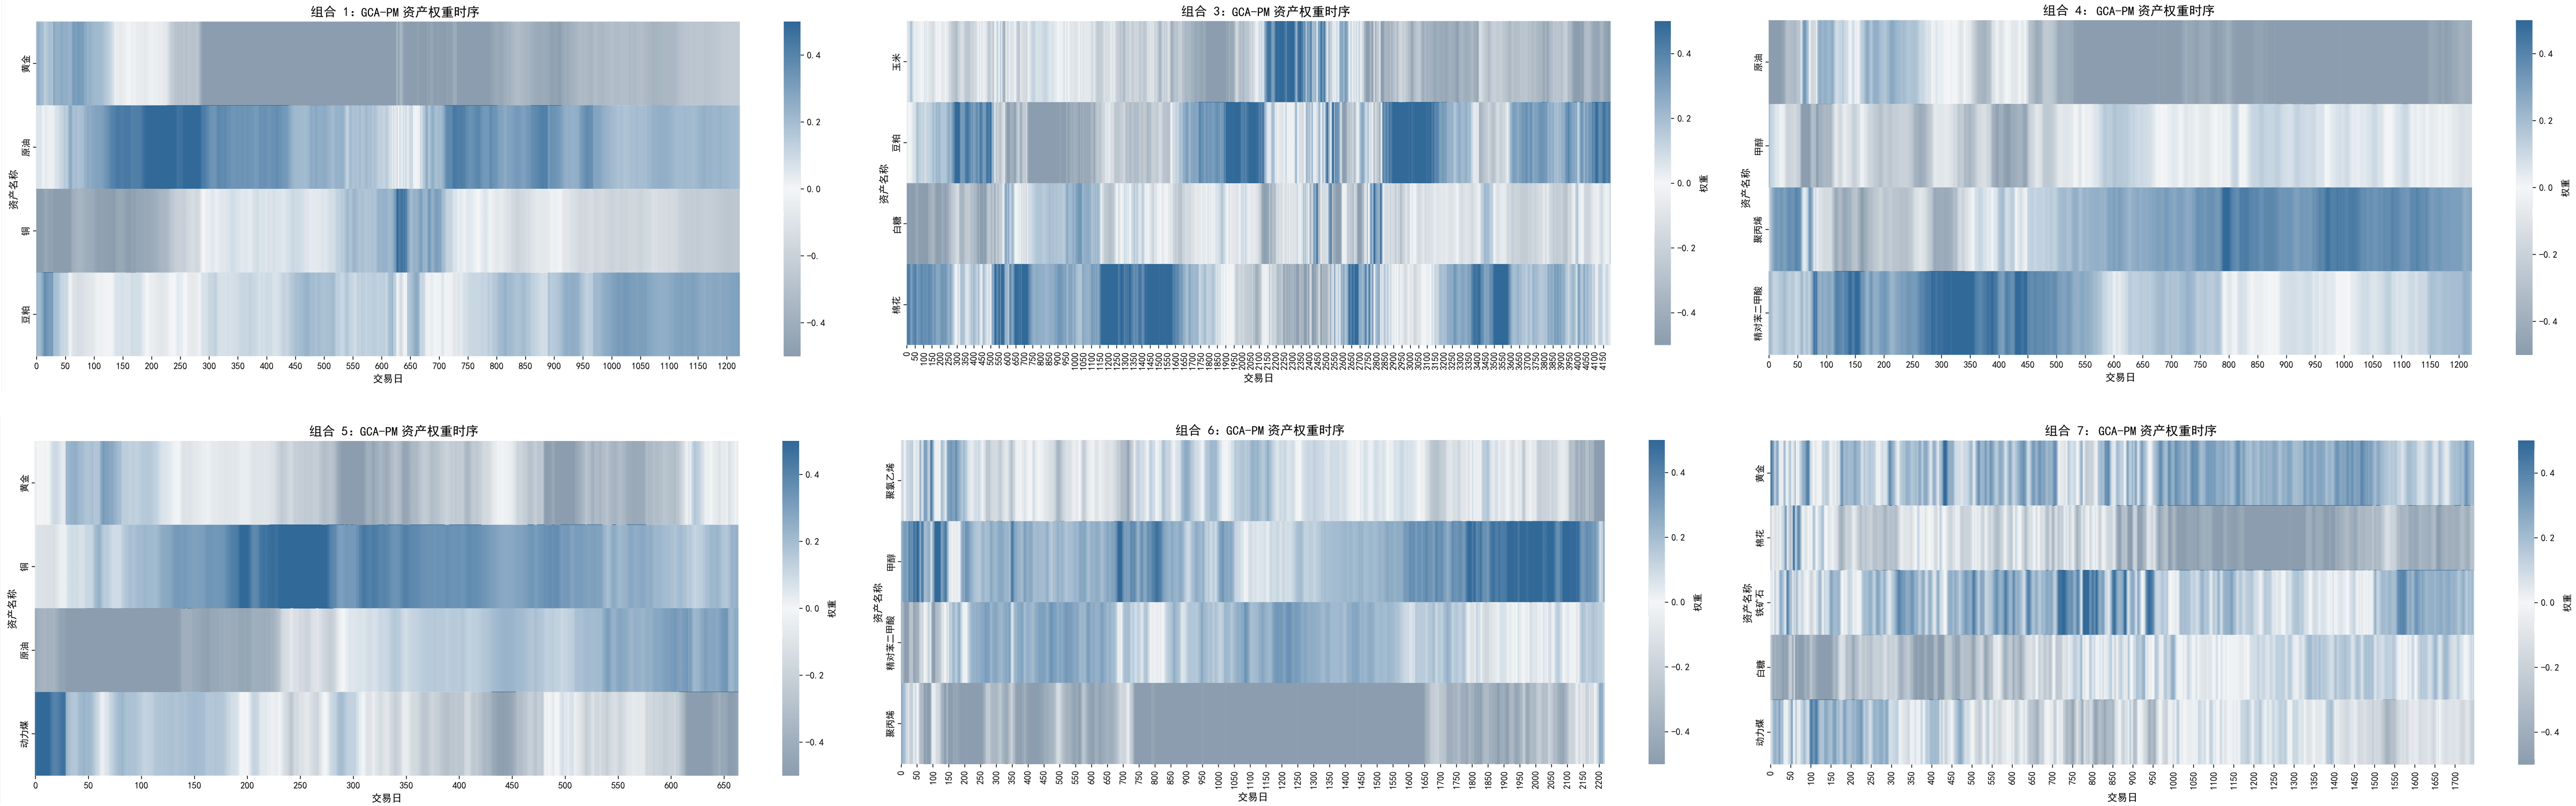
\includegraphics[width=0.95\textwidth]
    {figures/chap3/图2.8改.png}
    \caption{GCA 子智能体权重动态演化热力图}
    \label{fig:heatmap}
\end{figure}



\noindent\textbf{辅助校验层效果与权重动态分析}\par

为进一步观察辅助校验层的作用，本节通过夏普比率柱状图与权重热力图，从风险调整后收益和仓位动态两个维度进行说明。

% \subsubsection{夏普比率对比}

图 \ref{fig:qrgcasharpebar} 展示了 GCA 与辅助校验配置在六类实验组合上的夏普比率对比。

% \begin{figure}[htbp]
%     \centering
%     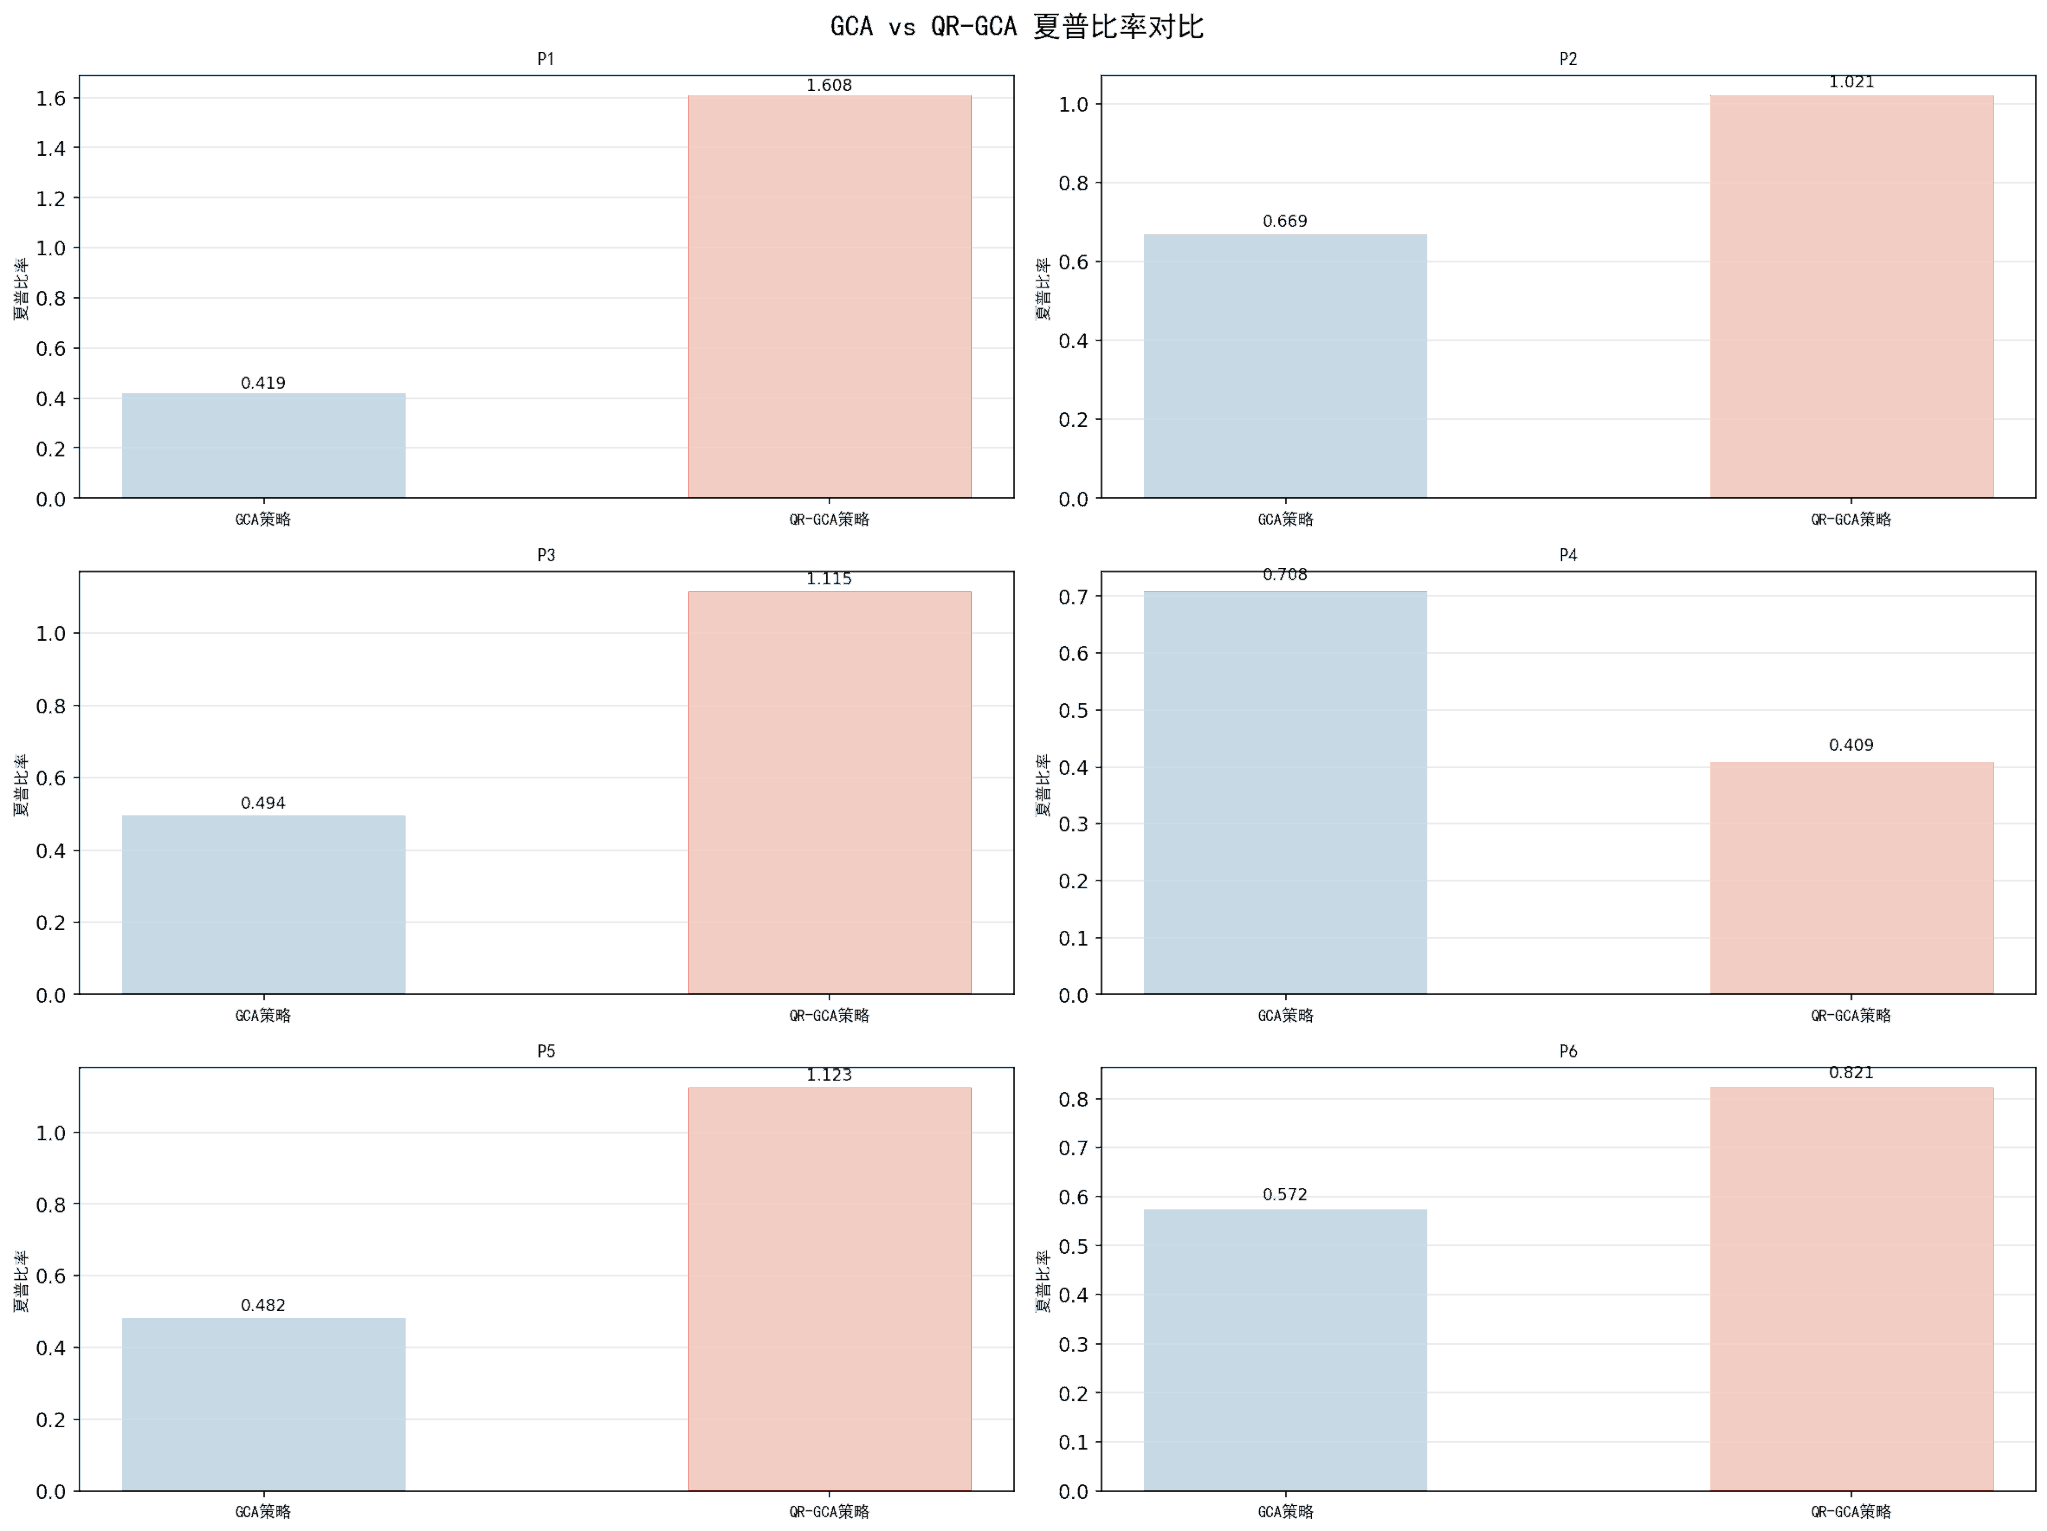
\includegraphics[width=0.95\textwidth]{figures/chap3/qr_gca/combined_qr_gca_sharpe.png}
%     \caption{GCA 与辅助校验层夏普比率对比}
%     \label{fig:qrgcasharpebar}
% \end{figure}

\begin{figure}[htbp]
    \centering
    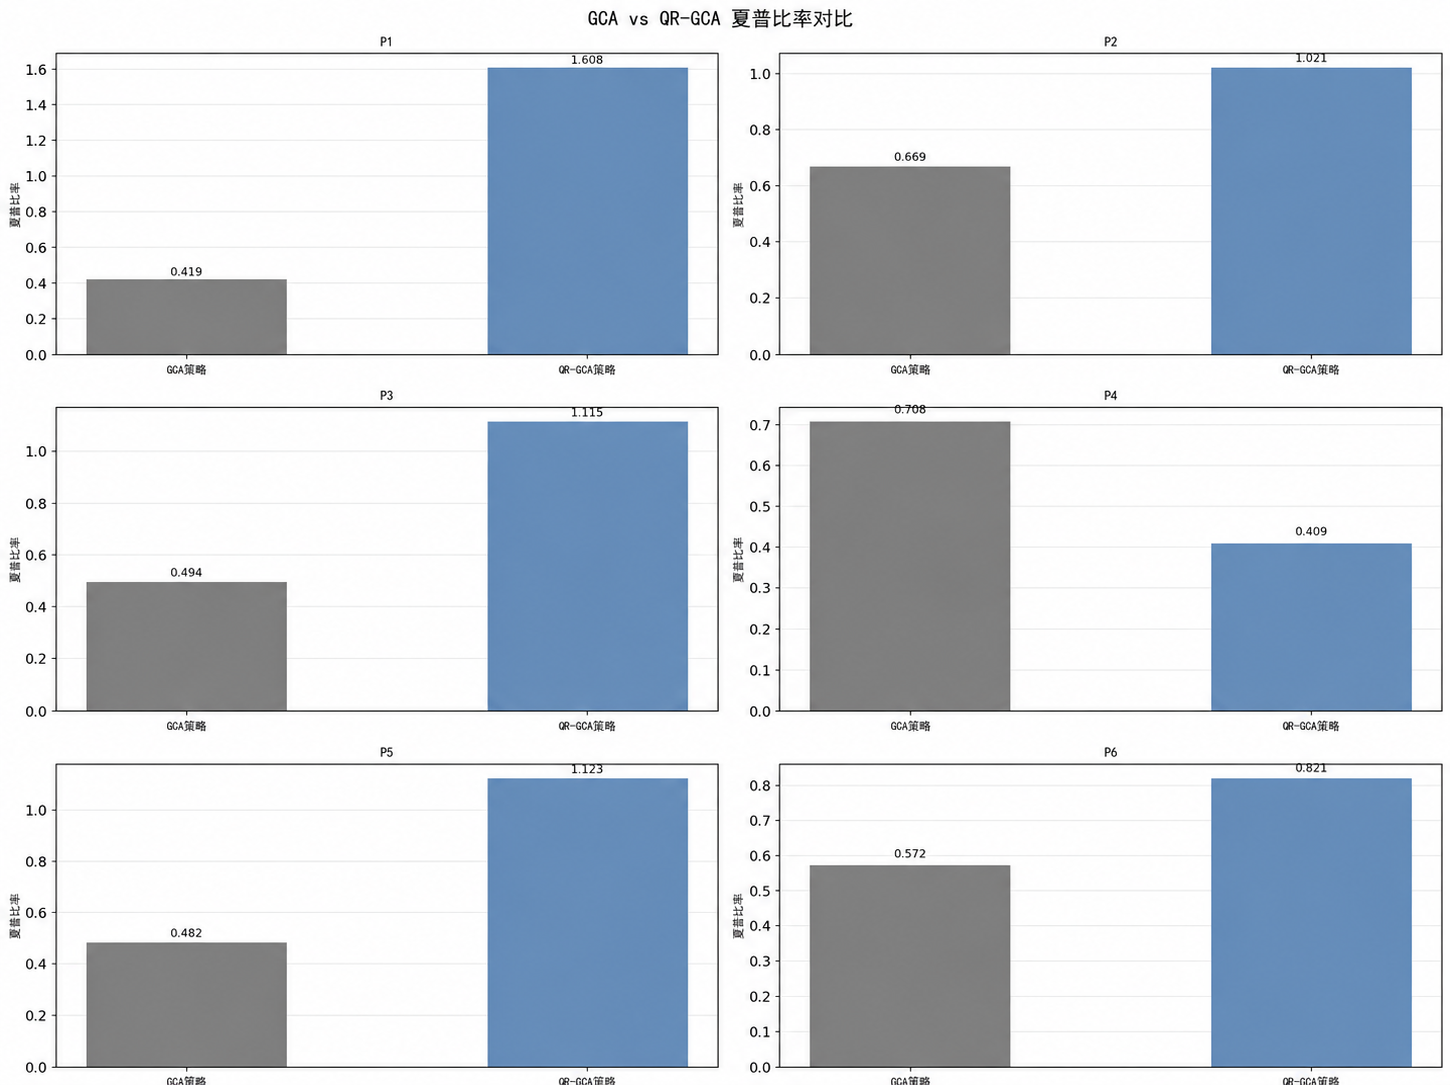
\includegraphics[width=0.95\textwidth]
    {figures/chap3/图2.9改.png}
    \caption{GCA 与辅助校验层夏普比率对比}
    \label{fig:qrgcasharpebar}
\end{figure}

% \begin{enumerate}
% \item \textbf{提升幅度的异质性}：
图 \ref{fig:qrgcasharpebar} 进一步显示，辅助校验层的效果具有组合差异：P1和P5提升幅度较大，P4则出现下降，说明统一市场状态过滤并不适用于所有组合。
% \end{enumerate}

% \subsubsection{辅助校验权重动态热力图}

图 \ref{fig:qrgcaheatmap} 展示了辅助校验层作用下的权重绝对值动态演化热力图。颜色越深表示该资产在对应时刻获得较大仓位，颜色越浅表示权重较低。

\begin{figure}[htbp]
    \centering
    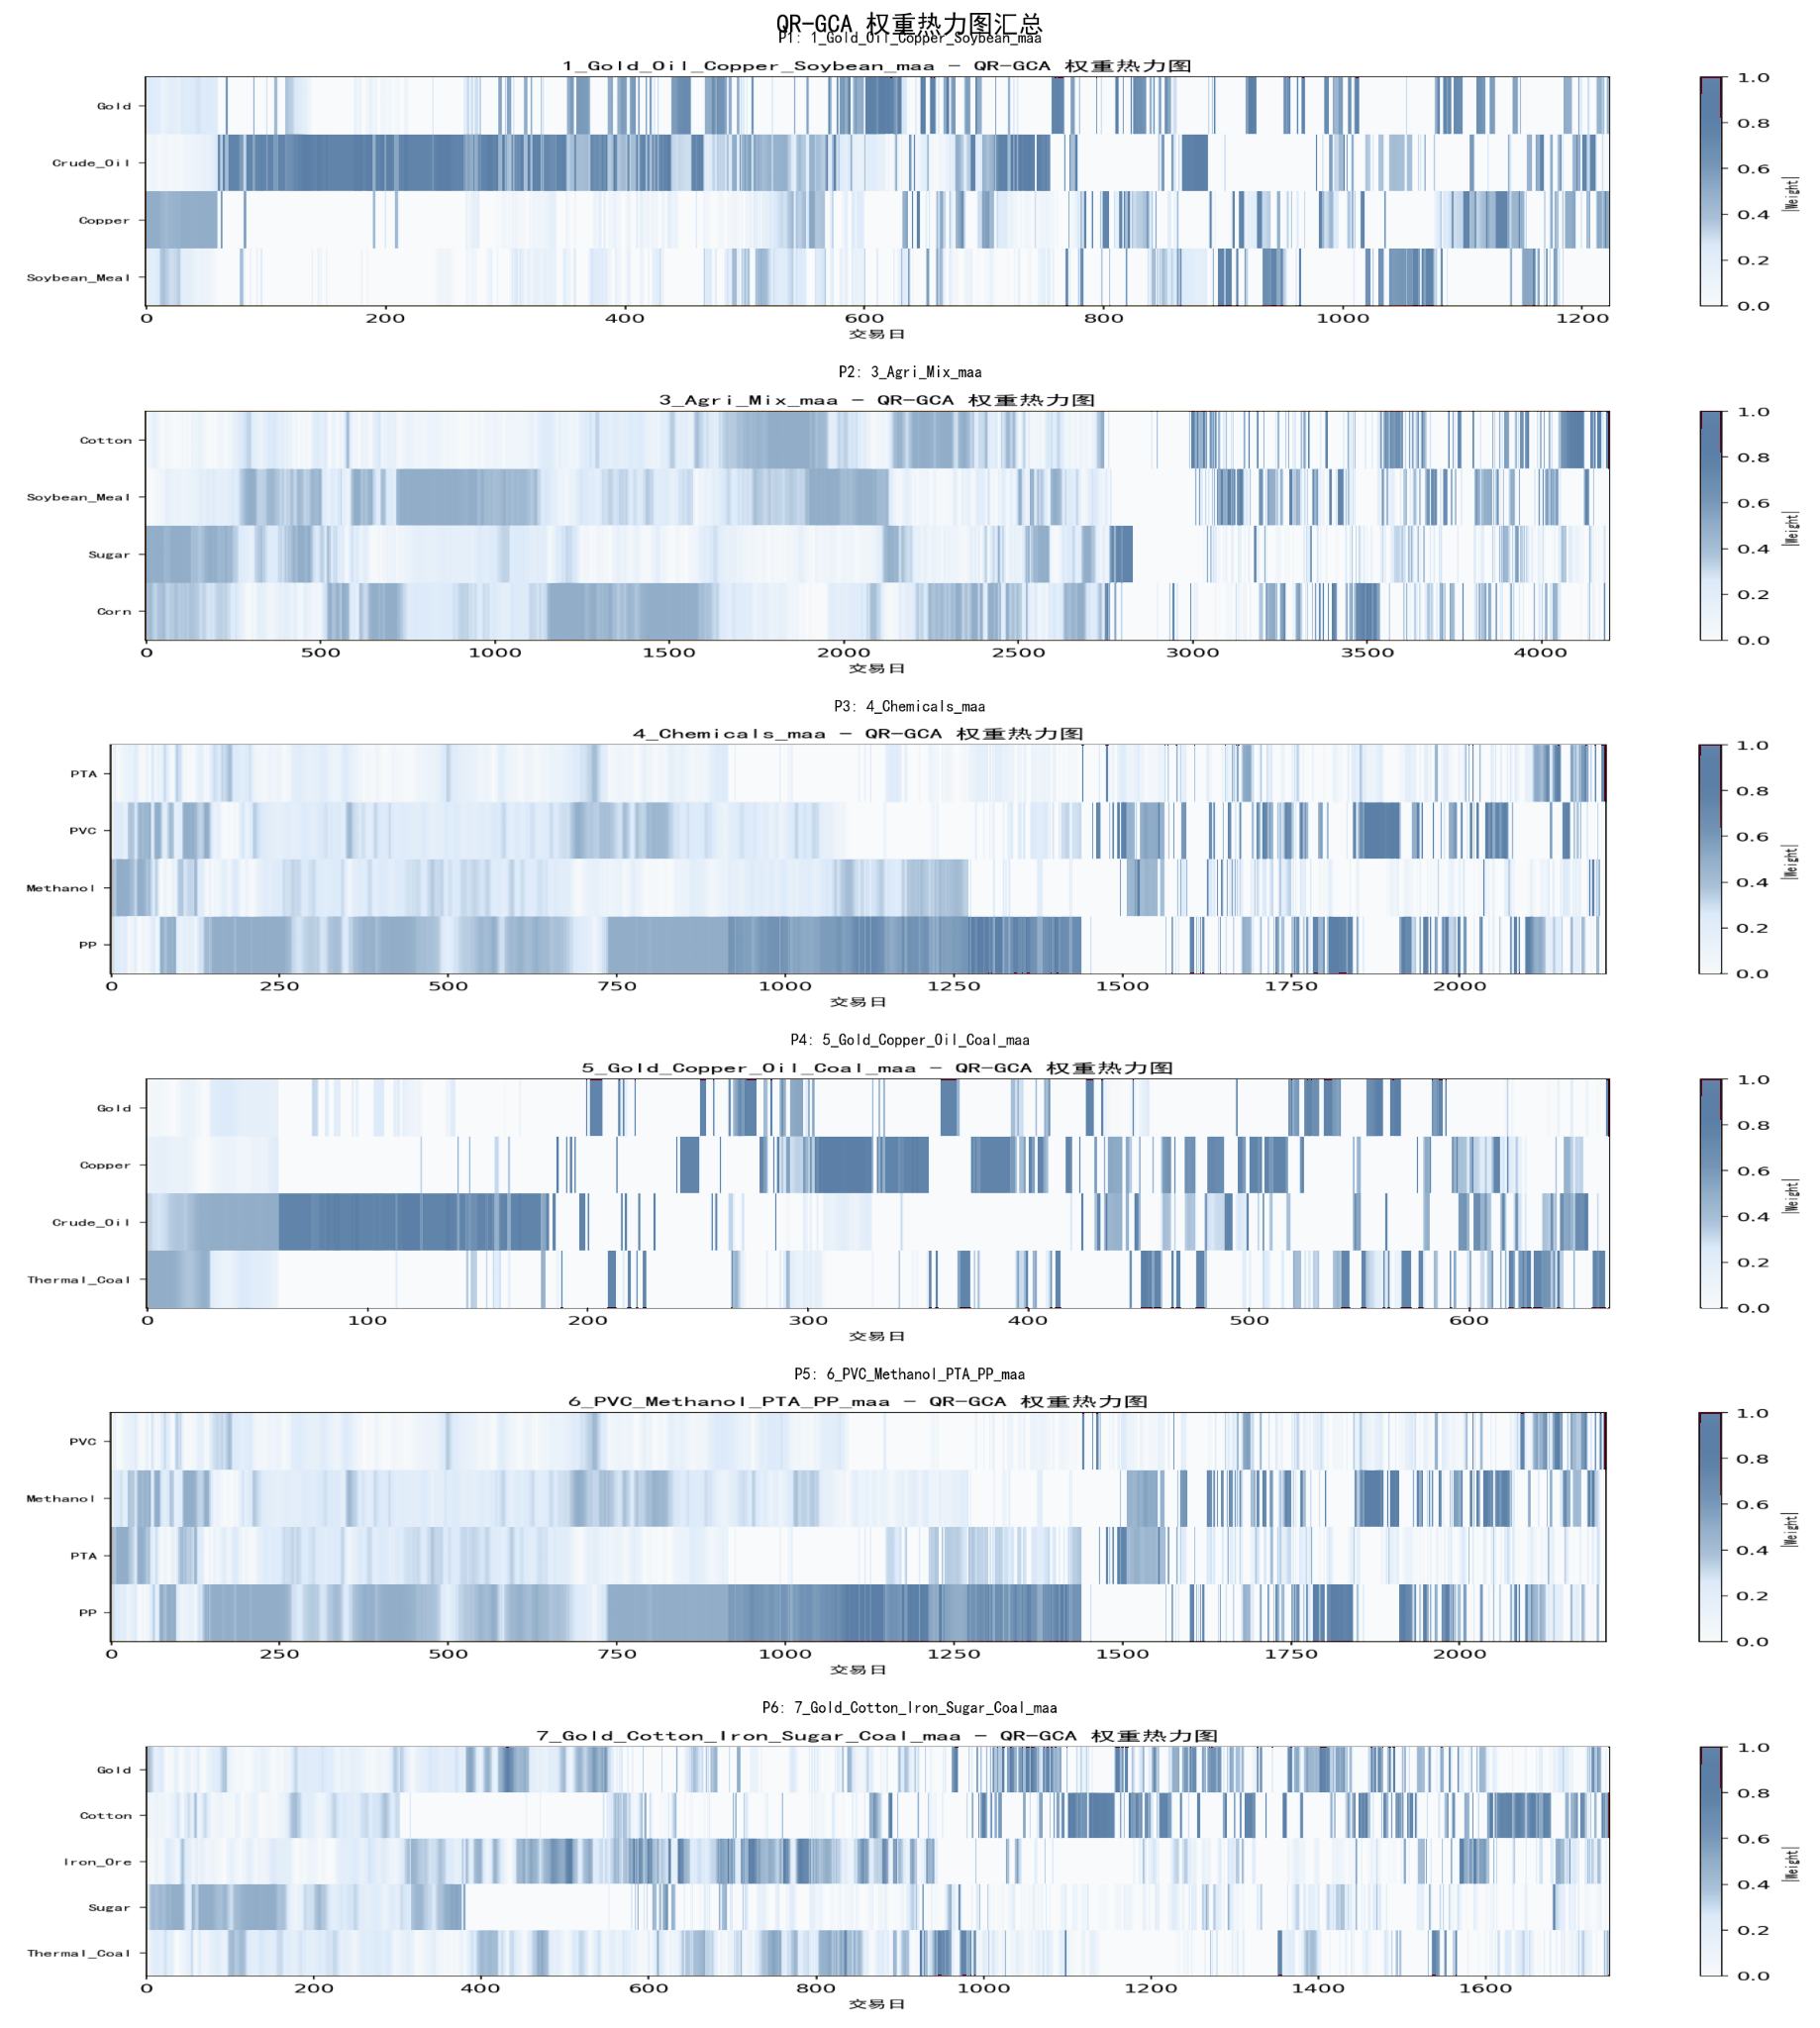
\includegraphics[width=0.95\textwidth]{figures/chap3/qr_gca/combined_qr_gca_weight_heatmap.png}
    \caption{辅助校验层权重动态热力图}
    \label{fig:qrgcaheatmap}
\end{figure}

图 \ref{fig:qrgcaheatmap} 显示，辅助校验层使仓位呈现一定稀疏性和阶段性。该结果说明其主要作用是减少震荡阶段的无效交易，并对GCA输出进行状态依赖的风险过滤。
% \end{enumerate}


\noindent\textbf{GCA消融实验及辅助接口贡献}\par
% 表~\ref{tab:experimental_results_summary}展示了各模块在六个实验组合上分别进行消融实验的数据结果。展示了所提出的各模块在六个不同数据集或实验组合上的消融实验结果。通过逐步引入GCA、S2T以及 Twin，模型的性能表现出了显著的动态变化，验证了各组件的有效性与协同作用。

% 在所有实验组合中，单纯的Baseline模型表现相对基础，其夏普比率、总收益及年化收益均处于较低水平，且部分组合（如P3和P5）甚至出现了负收益。引入图对比学习增强模块（GCA）后，在部分组合（如P1和P2）中观察到了初步的性能提升，但在其他组合（如P2、P3和P5）中却导致了收益回撤，表明单一的GCA模块在某些复杂场景下泛化能力有限。

% 然而，当进一步集成逆向师生蒸馏模块（S2T）后，模型性能获得了质的飞跃。在P2组合中，夏普比率从Baseline的0.3652提升至0.6279，总收益从60.61\%激增至105.73\%，且最大回撤从-21.17\%显著降低至-17.13\%。类似地，在P3和P6组合中，S2T模块的引入也大幅提升了收益指标并降低了风险。这证明了S2T模块在捕捉高维时序特征和降低波动性方面的关键作用。

% 最后，完整模型（Baseline-GCA-S2T-Twin）在绝大多数指标上均取得了最优表现。例如，在P3组合中，夏普比率进一步提升至0.5764，年化收益达到8.02\%，且最大回撤进一步压缩至-13.72\%；在P6组合中，夏普比率达到0.5613。随着模块的逐步叠加，换手率普遍呈现下降趋势（如P2组合从0.1538降至0.0397），表明所提出的模块能够生成更为稳健的交易信号，减少了不必要的频繁交易。

% 综上所述，消融实验结果明确表明，GCA模块为模型提供了基础的特征增强能力，S2T模块极大地提升了模型的收益风险比，而孪生对抗则进一步优化了模型的收敛性与稳定性，各模块协同工作显著提升了量化投资策略的整体性能。

% 表~\ref{tab:experimental_results_summary}展示了各模块在六个实验组合上分别进行消融实验的数据结果，系统性地验证了所提出的群组交叉对抗（GCA）、逆向师生蒸馏（S2T）及孪生对抗自体再生（Twin）模块在量化投资策略中的有效性与协同作用。实验数据表明，随着模块的逐步引入，模型性能呈现出显著的阶梯式提升，充分证明了各组件设计的合理性。
% 在所有实验组合中，单纯的Baseline模型表现相对基础，其夏普比率普遍低于0.4，总收益及年化收益均处于较低水平，且在P3和P5组合中甚至出现了负收益，暴露出模型在复杂市场环境下的局限性。引入图对比学习增强模块（GCA）后，在P1组合中观察到夏普比率从0.2168提升至0.2474，总收益从13.64\%增至15.85\%，表明GCA在部分场景下能够通过增强特征表达能力带来性能增益。然而，在P2、P3和P5组合中，GCA的引入反而导致收益回撤（如P5的总收益从-32.03\%降至-17.40\%），说明单一的GCA模块在处理高维非线性数据时泛化能力有限，可能因过度拟合局部特征而影响模型稳定性。

% 当进一步集成逆向师生蒸馏模块（S2T）后，模型性能获得了质的飞跃，尤其在风险收益平衡方面表现突出。在P2组合中，夏普比率从Baseline的0.3652跃升至0.6279，总收益从60.61\%激增至105.73\%，且最大回撤从-21.17\%显著降低至-17.13\%；在P3组合中，S2T模块将总收益从-12.51\%转正至12.82\%，最大回撤从-31.25\%压缩至-17.54\%，验证了S2T通过逆向师生蒸馏机制有效捕捉高维时序特征、抑制极端风险的能力。同时，S2T的引入并未显著增加换手率（P2组合从0.1538降至0.0479），表明其在提升收益的同时保持了交易策略的稳定性。

% 最后，完整模型（Baseline-GCA-S2T-Twin）在绝大多数指标上均取得了最优表现，体现了模块间的协同效应。在P3组合中，夏普比率进一步提升至0.5764，年化收益达到8.02\%，最大回撤进一步压缩至-13.72\%；在P6组合中，尽管GCA的引入导致性能下降，但完整模型通过S2T与Twin的协同补偿，使夏普比率达到0.5234，优于Baseline的0.4917。此外，随着模块的逐步叠加，换手率普遍呈现下降趋势（如P2组合从0.1538降至0.0397，P4组合从0.1287降至0.0408），表明GCA-S2T-Twin的联合优化能够生成更为稳健的交易信号，减少不必要的频繁交易，从而降低交易成本对策略收益的侵蚀。

% 综上所述，消融实验结果明确表明：GCA模块通过图对比学习为模型提供了基础的特征增强能力，但其泛化性能受限；S2T模块通过逆向师生蒸馏机制显著提升了模型的收益风险比，尤其在风险控制方面表现突出；而孪生对抗自体再生模块则通过对抗训练优化了模型的收敛性与稳定性，弥补了单一模块的不足。各模块的协同工作不仅实现了性能的叠加增益，更通过机制互补显著提升了量化投资策略的整体鲁棒性与适应性，为复杂金融时序数据的建模提供了有效解决方案。

表~\ref{tab:experimental_results_summary} 展示了不同配置在六个组合中的消融结果。整体上，基准模型在部分组合中表现不稳定；引入GCA后，模型获得多智能体交叉评估能力，但单一GCA并非在所有组合中都立即提升收益。继续接入知识传递和状态修复接口后，多数组合的夏普比率、最大回撤和换手率得到改善。需要注意的是，这些辅助接口在本章中的解释边界是“观察边际贡献”，而不是改变第二章的主体方法。该结果说明，GCA是本章面向投资组合管理的核心机制，辅助接口主要用于说明在GCA输出基础上进一步稳定训练状态和组合表现的可能性。



\begin{table}[H]
\centering
\caption{实验结果汇总表}
\label{tab:experimental_results_summary}
\small
\setlength{\tabcolsep}{3pt}
\renewcommand{\arraystretch}{1.15}
\begin{tabular}{@{}p{0.06\textwidth}p{0.34\textwidth}cccccc@{}}
\toprule
\textbf{组合} & \textbf{模型} & \textbf{夏普比率} & \textbf{总收益} & \textbf{年化收益} & \textbf{最大回撤} & \textbf{胜率} & \textbf{换手率}\\
\midrule
\multirow{4}{*}{\textbf{P1}} 
& 基准模型 & 0.2168 & 13.64\% & 2.81\% & -27.60\% & 49.63\% & 0.0760\\
& 基准模型-GCA & 0.2474 & 15.85\% & 3.27\% & -26.41\% & 49.63\% & 0.0713\\ 
& 基准模型-GCA-知识传递接口 & 0.3341 & 21.44\% & 4.42\% & -25.67\% & 49.63\% & 0.0444\\
& 基准模型-GCA-知识传递接口-状态修复接口 & 0.4532 & 28.87\% & 5.95\% & -20.34\% & 50.86\% & 0.0307\\
\midrule
\multirow{4}{*}{\textbf{P2}} 
& 基准模型 & 0.3652 & 60.61\% & 3.64\% & -21.17\% & 50.14\% & 0.1538\\
& 基准模型-GCA & -0.1990 & -16.40\% & -0.99\% & -33.07\% & 49.9\% & 0.1859\\
& 基准模型-GCA-知识传递接口 & 0.6279 & 105.73\% & 6.35\% & -17.13\% & 51.03\% & 0.0479\\
& 基准模型-GCA-知识传递接口-状态修复接口 & 0.6446 & 108.61\% & 6.53\% & -16.51\% & 50.86\% & 0.0397\\
\midrule
\multirow{4}{*}{\textbf{P3}} 
& 基准模型 & -0.2816 & -12.51\% & -2.58\% & -31.25\% & 48.41\% & 0.1600 \\
& 基准模型-GCA & -0.0976 & -6.53\% & -1.35\% & -22.23\% & 48.98\% & 0.1220\\
& 基准模型-GCA-知识传递接口 & 0.1936 & 12.82\% & 2.64\% & -17.54\% & 49.71\% & 0.0838 \\
& 基准模型-GCA-知识传递接口-状态修复接口 & 0.5764 & 38.91\% & 8.02\% & -13.72\% & 50.12\% & 0.0408\\
\bottomrule
\end{tabular}
\end{table}
\begin{table}[H]
\centering
{\small\textbf{续表}}\\[0.5em]
\small
\setlength{\tabcolsep}{3pt}
\renewcommand{\arraystretch}{1.15}
\begin{tabular}{@{}p{0.06\textwidth}p{0.34\textwidth}cccccc@{}}
\toprule
\textbf{组合} & \textbf{模型} & \textbf{夏普比率} & \textbf{总收益} & \textbf{年化收益} & \textbf{最大回撤} & \textbf{胜率} & \textbf{换手率}\\
\midrule
\multirow{4}{*}{\textbf{P4}} 
& 基准模型 & 0.6926 & 40.33\% & 15.31\% & -25.67\% & 49.70\% & 0.1287 \\
& 基准模型-GCA & 0.4158 & 24.14\% & 9.16\% & -29.29\% & 49.4\% & 0.1164\\
& 基准模型-GCA-知识传递接口 & 0.6814 & 39.49\% & 14.99\% & -24.23\% & 48.49\% & 0.0638 \\
& 基准模型-GCA-知识传递接口-状态修复接口 & 0.7120 & 40.45\% & 15.35\% & -23.95\% & 47.89\% & 0.0408\\
\midrule
\multirow{4}{*}{\textbf{P5}} 
& 基准模型 & -0.3512 & -32.03\% & -3.64\% & -49.91\% & 48.51\% & 25.66\%\\
& 基准模型-GCA & -0.2657 & -17.40\% & -1.98\% & -34.01\% & 48.96\% & 0.3665\\
& 基准模型-GCA-知识传递接口 & 0.2701 & 23.62\% & 2.68\% & -26.5\% & 49.64\% & 11.13\%\\
& 基准模型-GCA-知识传递接口-状态修复接口 & 0.4407 & 38.28\% & 4.35\% & -21.22\% & 50.95\% & 4.82\%\\
\midrule
\multirow{4}{*}{\textbf{P6}} 
& 基准模型 & 0.4917 & 45.72\% & 6.59\% & -16.17\% & 52.00\% & 0.0939\\
& 基准模型-GCA & 0.3817 & 35.09\% & 5.06\% & -18.31\% & 51.32\% & 0.1120\\
& 基准模型-GCA-知识传递接口 & 0.5613 & 52.00\% & 7.50\% & -13.61\% & 51.37\% & 0.0751 \\
& 基准模型-GCA-知识传递接口-状态修复接口 & 0.5234 & 49.12\% & 7.08\% & -13.97\% & 50.97\% & 0.0835\\
\bottomrule
\end{tabular}
\end{table}

\vspace{1em}
%\textit{注：表中数据为样本外测试集结果，"—"表示未适用。}

% \subsection{实验小结}

% 本节针对 多智能体群组交叉对抗框架与辅助校验层信号增强机制进行了系统的实证验证。基于上述实验结果，可以得出以下关键结论：
% % \begin{enumerate}
% % \item \textbf{基础模型优势}：
% MGCA 在六大投资组合上均展现出优于单一基准模型（GRU、LSTM、Transformer）的风险调整后收益表现，特别是在高波动环境和多元低相关场景下表现突出；
% % \item \textbf{辅助校验效果}：
% 辅助校验层信号增强机制在多数组合上实现了夏普比率的显著提升，验证了信号级融合的有效性；
% % \item \textbf{模块贡献}：
% 消融实验验证了异构生成器、交叉对抗机制及组内/全局蒸馏各模块的独立贡献；
% % \item \textbf{损失函数作用}：多目标损失配置实验表明，MSE、GAN 与 Sharpe 三者的协同作用优于任一单一损失函数；
% % \item \textbf{适用边界}：
% 辅助校验层在避险对冲型组合中效果不佳，揭示了组合指数状态判别机制的适用边界。
% % \end{enumerate}

% \textit{注：详细的实验数据请参照表 \ref{tab:experimental_results_summary}、表 \ref{tab:ablation_study} 及表 \ref{tab:loss_config_comparison}，待实验完成后填充。}


% \section{讨论}

% \subsection{MGCA 有效性的归因}

% 多智能体群组交叉对抗框架在多个异构资产组合中展现出的显著优势，并非来自单一组件的堆砌，而是源于其在 架构归纳偏置、博弈正则化 与 经济学对齐 三个维度的深度整合：
% 架构归纳偏置方面的时序-架构的物理对齐
% 不同于传统的集成学习，MGCA 构建了具有物理意义的异构分工机制。模型根据已知的归纳偏置（Inductive Bias）分配计算资源：GRU被指派处理高频微观结构（5日窗口），利用其门控循环单元快速响应短期反转；Transformer 被指派处理宏观趋势（20日窗口），利用自注意力机制捕获跨月度的结构性关联。这种“各司其职”的设计使得模型能够同时捕捉瞬态的 Alpha 信号与持久的 Beta 趋势。

% 博弈正则化中
% 多个判别器构成的动态博弈环境充当了强大的正则化器。对抗损失 $\mathcal{L}_{adv}$ 本质上是在通过最小化生成分布与真实分布的 JS 散度，迫使生成器学习隐含的市场状态转移概率。这种机制有效过滤了样本中的高斯白噪声，显著降低了过拟合风险（表现为 P5 组合中 GRU 崩溃而 MGCA 存活）。

% 从经济学目标导向上分析Sharpe Ratio Loss的端到端集成，完成了从“预测价格”到“预测收益质量”的范式转变。该损失函数作为一种隐式的风险过滤器，引导梯度流向那些方向准确且波动率可控的特征子空间。这种协同作用使得 MGCA 展现出审慎的风险控制特征：在充满不确定性的震荡市（如 P1）保持低换手率以保存资本，而在趋势明朗的结构性行情（如 P2）中果断放大在大类资产上的风险敞口。



\section{本章小结}

本章围绕对冲基金交易流程中的投资组合管理环节，提出并验证了面向投资组合管理的群组交叉对抗学习方法（GCA）。本章首先从传统投资组合管理方法的局限性和金融场景下多智能体博弈建模挑战出发，说明多资产配置中存在信号不稳定、模型输出趋同、组合权重偏差和风险约束难以统一等问题；随后在“任务描述”部分，将本章任务明确为多资产收益预测、组合权重生成和风险调整收益约束下的配置决策问题。由此，本章对资产配置对象选择的讨论并不止于识别单个资产的上涨概率，而是进一步落实为在多资产之间形成相对稳定、可约束、可执行的资金配置方案。

在方法设计层面，GCA将一对一的生成器—判别器博弈扩展为多生成器、多判别器之间的群组交叉对抗。异构生成器基于不同归纳偏置提取多尺度市场特征，判别器通过跨生成器评估约束预测输出的分布一致性，从而降低单一模型在复杂资产池中产生的配置偏差。量化相对强度指标在本章中仅作为GCA输出后的辅助校验量，用于观察权重过滤对交易可用性的影响，不替代GCA主体方法。知识传递和状态修复接口也仅在消融实验中作为辅助配置出现，用于观察其对GCA训练稳定性和组合表现的边际影响；其具体机制与章节主体任务将在后续章节分别展开。

实验部分基于六类差异化资产组合开展样本外回测。实验结果显示，GCA在多数实验组合中相较单一架构基准模型表现出更稳定的风险调整收益与回撤控制特征。辅助接口和输出校验层在部分组合中进一步改善了组合表现，但其作用具有场景边界，不能替代GCA在本章中的核心地位。总体而言，本章的贡献在于把多智能体交叉博弈机制落实到投资组合管理场景中，使预测信号经过分布校验、相对收益比较和风险约束后转化为组合权重，而不是停留在单资产预测精度提升层面。

因此，本章对应交易决策链条中的投资组合管理环节，围绕资产配置对象选择和资金配置建立GCA方法及其组合权重生成机制。后续第3章转向高维金融因子建模，进一步讨论资产配置背后的因子依据；第4章讨论时序结构识别，第5章讨论交易执行优化，第6章则面向策略整合与最终交易判断。
 %第二章
     \chapter{面向高维金融因子建模的赛马场竞争方法}

\section{问题的提出}
在对冲基金交易决策链条中，第2章已经围绕多资产配置对象识别与资金权重生成问题展开讨论。然而，资产配置结果能否成立，并不只取决于模型是否给出某一组权重，还取决于这些权重背后是否存在稳定、可解释且能够跨市场状态迁移的因子依据。换言之，第3章关注的重点并不是对资产选择作事后说明，而是在高维金融因子空间中识别能够持续支撑资产配置判断的有效信息。

高维金融因子建模因此成为连接资产配置与后续时机判断的重要中间环节。金融市场中的价格与收益并不是由单一线性信号决定的，而是受到交易机制、信息结构和市场参与者行为的共同影响。异质信息交易条件下的买卖价差与成交价格研究说明，价格序列本身已经包含了交易摩擦和信息不对称因素\cite{glosten1985bid}。连续竞价与内幕交易模型进一步表明，市场价格形成过程会受到交易者信息优势和交易冲击的影响\cite{kyle1985continuous}。因此，高维金融因子建模面对的并不只是变量数量过多的问题，还包括不同信息来源在时间维度、资产维度和市场状态维度上的交互关系如何被稳定识别的问题。

在这一背景下，传统降维方法虽然能够在一定程度上压缩变量空间，但在面对高度非线性、强噪声和多源异构的金融因子时，往往难以充分保留因子之间的复杂交互关系。近年来，深度学习和强化学习方法被引入时间序列预测与多因子建模任务，为非线性因子表征提供了新的工具。金融交易中的合成数据增强与深度强化学习研究说明，深度模型可以借助状态扩展和序列决策机制捕捉部分传统线性方法难以表达的动态关系\cite{liu2022synthetic}。不过，高维因子建模的困难并不只在于表达能力不足，还在于模型面对扰动、噪声和分布漂移时能否保持稳健。鲁棒对抗强化学习研究表明，引入对抗扰动有助于检验和提升策略在复杂环境中的稳定性\cite{pinto2017robust}。这也提示本文，第三章不能只依赖单一深度模型的拟合能力，而需要进一步设计能够持续比较、筛选和修正因子表征的动态竞争机制。

从方法论上看，主成分分析的基本作用是将原始变量投影到少数主成分空间，适合概括线性相关结构，但并不能直接完成金融因子的可交易性筛选\cite{abdi2010principal}。因此，本章关注的关键问题是：在高维、强噪声和非平稳环境下，如何通过动态竞争机制持续筛选有效因子表征，并避免模型群体过早收敛到单一、脆弱的因子解释路径。


\subsection{高维金融因子的非对称竞争关系}
在第2章完成投资组合管理任务并形成多资产配置入口之后，本章进一步将研究对象转向资产配置背后的因子依据层面。对于多资产交易任务而言，组合权重并不是孤立生成的结果，而是建立在一组能够解释收益来源、风险暴露和市场状态变化的候选因子之上。因此，本节关注的不是简单增加因子数量，也不是仅对原始变量进行压缩，而是讨论高维金融因子在不同市场环境下为何会呈现强弱差异、替代关系和阶段性失效。换言之，高维金融因子并不是同质变量集合，不同因子对收益预测、风险识别和资产选择的贡献存在明显差异，这构成了后续赛马场竞争机制需要处理的基本问题。

从方法层面看，传统降维方法能够压缩变量空间，但其主要目标通常是保留总体结构、局部邻近关系或方差贡献，并不直接等同于筛选具有交易含义的金融因子。相关降维评估研究表明，高维数据在降维过程中容易出现结构信息损失和局部关系扭曲的问题\cite{espadoto2019toward}。这一问题在金融因子场景中会被进一步放大，因为部分因子虽然总体方差贡献并不突出，却可能在特定市场状态、极端行情或风险切换阶段具有较强解释价值。因而，如果只依赖静态降维结果判断因子重要性，可能会将短期波动较弱但交易含义明确的变量提前压缩掉。

静态深度表示模型在一定程度上缓解了线性降维的表达能力不足问题。表示学习研究说明，深度模型可以通过多层非线性变换学习复杂数据表征\cite{bengio2013representation}。但是，在金融市场中，表征能力增强并不必然意味着因子解释路径稳定。模型可能在训练样本中捕捉到局部有效的非线性组合，却难以保证该组合在样本外、跨周期或不同资产类别之间持续有效。因此，本章所讨论的高维因子建模，不只是寻找更复杂的表示函数，而是需要判断不同候选因子在动态市场环境中是否仍具备稳定的解释力和可迁移性。

进一步看，不同金融因子之间并非始终保持平等、独立和静态的关系。某些因子在趋势行情中具有较强预测能力，却可能在震荡行情中失效；某些因子单独使用时贡献有限，但与波动率、流动性或基本面变量组合后能够增强风险识别能力；还有一些因子在样本内表现突出，却可能只是由特定时期的偶然相关驱动。演化博弈相关研究为理解主体之间的动态竞争和策略调整提供了可借鉴视角\cite{chang2025survey}。借助这一视角可以看到，高维因子空间中的有效信息并不是一次性固定下来的，而是在不同市场状态下持续发生相对强弱变化。所谓非对称竞争，正是指不同因子在信息含量、稳定性、可解释性和适用场景上并不均衡，其竞争结果会随市场环境变化而调整。

从金融含义上看，因子不是普通统计变量，而是与风险补偿和收益来源相联系的结构化特征。经典多因子模型将股票与债券收益分解为共同风险因子，为高维因子建模提供了资产定价层面的基础参照\cite{fama1993common}。这说明，因子筛选不能只看统计拟合效果，还要说明该因子是否对应可解释的风险暴露或收益来源。五因子模型进一步把盈利能力、投资等维度纳入收益解释框架，表明有效因子往往同时具有统计有效性和经济含义\cite{fama2014five}。因此，在本章语境下，因子竞争并不是单纯比较预测误差大小，而是比较不同因子表征能否持续支撑资产配置判断、风险解释和后续时序结构识别。

随着候选因子数量不断扩展，“因子动物园”问题会进一步放大冗余特征、偶然相关和多重检验风险。因此，因子筛选不能只依赖样本内拟合表现，还需要关注其跨周期稳定性与经济解释能力\cite{feng2020taming}。这一点对本章尤为重要：如果模型只在大量候选因子中寻找短期最优组合，就可能把偶然有效的弱相关变量误判为稳定因子；如果模型只保留传统意义上的主导变量，又可能忽略在局部行情中具有边际贡献的长尾因子。因而，高维因子建模需要在“防止冗余因子干扰”和“保留潜在有效弱信号”之间取得平衡。

金融市场的非平稳性进一步加剧了这种平衡的难度。资产收益及其特征结构会随着宏观环境、交易制度、市场情绪和风险补偿机制的变化而不断调整。资产定价中的因子学习研究说明，因子暴露和收益解释关系并不是固定不变的\cite{KELLY2019501}。对本章而言，这一结论强调的是因子有效性本身具有状态依赖性：同一因子在不同市场阶段可能对应不同的收益解释和风险补偿含义。相关研究也提示，金融预测中的有效特征会受到样本区间和市场状态变化的影响\cite{repec:fau:wpaper:wp2024_26}。由此可见，因子层面的暴露变化与特征层面的有效性变化会共同影响模型对候选因子的筛选判断。这意味着，在某一阶段表现较强的因子，可能在市场状态转换后迅速退化；而在常规区间中不显著的因子，也可能在极端行情或结构切换阶段提供额外信息。

在这种背景下，依赖固定表示结构的静态模型一旦遭遇分布漂移，容易出现样本外泛化能力下降的问题。分布变化与泛化研究说明，当训练分布和测试分布之间存在偏移时，模型需要关注跨环境稳定性，而不能只依赖单一样本分布下的拟合结果\cite{scholkopf2021toward}。对应到金融因子建模中，这意味着模型不仅要识别当前样本中最强的因子组合，还要避免过早排除在未来状态中可能重新发挥作用的候选因子。高维估计误差也会进一步传导到后续组合权重与风险暴露之中。协方差收缩研究表明，在样本有限且变量维度较高时，直接使用样本协方差矩阵容易导致估计不稳定\cite{ledoit2004honey}。这一问题首先体现为风险结构估计的不稳定：因子之间的协方差关系一旦被噪声放大，后续组合权重就可能对局部样本特征过度敏感。参数估计误差所引发的组合优化困境也说明，样本内最优并不必然对应样本外稳健\cite{michaud1989markowitz}。因此，高维因子建模不仅要关注因子本身的预测能力，还要关注其估计误差是否会在组合优化环节被进一步放大。

因此，高维金融因子建模的关键困难，并不只是对静态样本进行拟合，而是如何在分布持续变化的环境中识别仍具有解释力和预测价值的因子结构。深度学习与强化学习在金融交易中的应用表明，序列模型和状态扩展机制能够帮助模型捕捉部分传统线性方法难以表达的动态关系\cite{liu2022synthetic}。但是，单一模型即使具备较强非线性表达能力，也难以保证其因子表征始终稳健。基于上述分析，本章引入赛马场竞争机制，并将其定位为一种面向高维因子空间的动态筛选逻辑：通过模型群体之间的持续比较、更新和知识迁移，识别在不同市场状态下相对稳定且具有解释意义的因子表征。与第2章侧重投资组合管理和资产配置不同，本章重点说明资产选择背后的因子依据如何形成，并为后续时序结构识别提供更可靠的输入基础。

\subsection{传统因子建模中的过早收敛困境}
上一节从因子层面说明了高维金融因子并非同质变量集合，不同因子在收益解释、风险暴露和市场状态切换中的作用存在非对称差异。进一步看，即使模型具备较强的非线性表达能力，训练过程本身也可能放大这种非对称性：早期被模型捕捉到的强信号会在后续迭代中被持续强化，而弱幅度但具有解释价值的长尾因子、阶段性因子和跨周期因子则可能被过早压缩或排除。由此形成的过早收敛，并不是简单的训练轮次不足问题，而是模型在高维因子空间中提前固化到局部有效解释路径的问题。

传统依赖线性假设的特征工程方法，在刻画高维金融变量之间的非线性依赖关系及复杂联合分布时存在明显局限。深度生成模型为高维表征学习提供了新的工具，其中变分自编码器通过潜变量建模与变分推断，能够从高维数据中学习连续且具有结构性的隐表示\cite{kingma2014autoencoding}。这种潜变量思想说明，高维因子可以被压缩到更紧凑的表示空间中，但潜变量压缩解决的是表示组织问题，并不直接等同于有效因子的持续筛选；压缩后的表示是否保留稳定的金融解释，仍需要结合收益预测、风险暴露和跨周期表现进一步判断。随机反向传播与近似推断方法为深度生成模型中的潜变量学习提供了可训练路径\cite{rezende2014stochastic}。这种可训练性使模型能够在高维因子空间中形成潜在表示，但训练目标仍主要围绕重构质量和潜在分布约束展开。其目标函数通常由重构项与基于库尔贝克—莱布勒散度的正则项共同构成\cite{kullback1951information}。这类正则约束有助于稳定潜在空间，但在金融场景中，平滑的潜在分布并不必然意味着弱信号、长尾信号和跨周期信号能够被持续保留。与以重构和潜在空间正则为主的模型不同，生成对抗网络进一步把分布学习放入生成器与判别器之间的博弈过程中，在非线性分布拟合与样本生成方面展现出较强能力\cite{goodfellow2014generative}。不过，对抗学习强调分布匹配，仍需进一步回答模型是否会在训练早期过度强化少数短期占优的因子表征，以及这类表征能否在市场状态变化后得到及时校正。

在更具体的金融时序预测任务中，堆叠自编码器与长短期记忆网络相结合的研究说明，深度表示学习可以从复杂价格序列中提取非线性特征，并为后续预测任务提供更丰富的状态表达\cite{ding2020deep}。这类方法表明，非线性表征能够改善部分金融预测任务，但其重点仍主要落在单个模型在固定训练流程中的表达能力上。对于本章而言，更关键的问题并不是模型能否拟合复杂序列，而是当候选因子数量较多、市场状态不断切换时，模型群体能否持续比较不同因子路径的有效性，并避免所有模型同时收敛到同一类短期强信号。

金融时间序列通常表现出尖峰厚尾、波动聚集和分布偏移等特征，这使得生成模型的训练稳定性本身也成为重要问题。相关研究从目标函数和距离度量角度改进生成对抗训练，为缓解分布学习过程中的不稳定性提供了思路\cite{arjovsky2017towards}。这一类方法说明，改变分布度量可以改善训练过程，但它主要解决的是对抗学习能否稳定推进的问题，而不是高维因子是否被持续筛选的问题。梯度惩罚机制被用于增强Lipschitz约束，从而改善对抗训练的稳定性与鲁棒性\cite{gulrajani2017improved}。这提示本文，训练稳定性是必要条件，但如果模型结构和更新规则缺少差异化竞争，稳定训练也可能只是稳定地强化既有优势路径。扩散模型通过逐步去噪过程学习数据分布，为复杂分布建模提供了新的思路\cite{ho2020denoising}。然而，复杂分布建模能力的提升仍不等于动态因子筛选机制的形成，尤其不能自动保证弱信号、长尾信号和跨周期信号在训练过程中被保留。

从潜在表示与金融定价结合的角度看，对抗自编码器将重构学习与对抗训练结合起来，使潜在表示在重构观测数据的同时更接近预设先验分布\cite{makhzani2015adversarial}。这类方法对于高噪声数据的潜在表示学习具有启发意义，但其核心仍是使潜在空间更加规整，而不是直接刻画因子之间的动态竞争关系。联合编码与生成的对抗表示学习方法进一步增强了潜变量与观测数据之间的协调性\cite{donahue2017adversarial}。这种协调性对于金融数据建模具有参考价值，但在非平稳市场中，观测数据与潜变量之间的对应关系会随市场状态变化而改变，因而仍需要后续机制持续检验表征是否过早固化。

在资产定价场景中，带工具变量的主成分分析尝试从资产特征中学习条件风险暴露，为高维因子提取提供了更贴近金融问题的统计框架\cite{kelly2020instrumented}。自编码器资产定价模型也说明，非线性表示学习可以用于从大量资产特征中提取潜在定价结构\cite{gu2021autoencoder}。这两类研究表明，深度表示并非脱离金融含义的纯技术工具，而可以服务于风险暴露和资产定价结构的识别。进一步看，面向数字金融网络经验资产定价的多空双模式知识蒸馏框架说明，模型间知识传递不仅可用于压缩模型，也可服务于多空结构下的因子表征迁移\cite{yi2024longshort}。但是，知识迁移本身也存在方向性风险：若成熟模型已经过度依赖旧市场状态下的优势因子，直接传递其表征可能会把既有偏差延续到新模型之中；若新生模型的差异化探索缺少反向约束，又可能引入噪声因子并破坏已有稳定表征。因此，知识传递必须与动态竞争、筛选和校正机制结合，才能真正缓解过早收敛。

然而，金融时间序列具有较强的非平稳性与分布漂移特征，训练阶段学习到的分布结构往往难以直接推广到新的市场环境中。分布鲁棒优化研究从不利分布扰动下的泛化角度说明，模型训练不能只依赖单一经验分布下的拟合表现\cite{sagawa2020distributionally}。针对时间序列生成任务，时间序列生成对抗网络将对抗学习与时间监督机制结合，用于保留序列的动态依赖结构\cite{yoon2019time}。这些研究共同提示，金融时序建模既需要复杂表征能力，也需要对分布变化和动态依赖保持敏感。基于这一背景，本章关注的不是单个模型拟合能力的继续堆高，而是在高维因子空间中建立“非对称竞争—过早收敛识别—动态选优修正”的训练闭环，使有效因子能够在模型群体的持续竞争中被筛选、保留和更新。


\section{相关工作}
围绕高维金融因子建模，已有研究主要集中在统计降维、深度表示学习与多模型集成三个方向。统计降维方法侧重压缩变量空间，深度表示学习方法强调非线性特征提取，多模型集成方法则利用模型差异性改善预测稳定性。这些研究构成了金融因子建模的重要基础，但在非平稳市场环境下，仍然容易出现因子表征固化、有效因子与噪声因子难以持续区分、模型群体缺乏动态更新机制等问题。

在量化投资研究中，机器学习驱动的基本面量化投资已经被用于刻画资产特征、基本面变量与投资决策之间的关系\cite{li2019machine}。这类研究说明，机器学习方法能够拓展传统因子建模的变量空间和非线性表达能力，但也进一步凸显出一个问题：当候选特征数量持续增加时，因子筛选不能只依赖一次性训练结果，而需要能够持续区分有效信息、冗余信息和噪声信息的动态机制。

从本章研究对象看，相关工作的关键不足并不只是单一模型表达能力有限，更在于模型群体缺少持续筛选、更新和知识传递机制。当市场状态发生切换时，静态集成或固定权重组合容易在已有优势路径上停留过久，进而形成过早收敛。此时，模型可能继续强化样本内表现较好的局部因子结构，却难以及时识别新的市场状态和长尾因子信息。

为了克服单一模型在复杂分布下的局限性，多模型协作与集成学习逐渐成为研究热点\cite{yuan2021self}。然而，现有的多模型方法大多缺乏明确的动态淘汰与知识转移机制，模型之间的差异性难以长期保持。主动管理基本定律强调，多个弱信号需要在信息质量与独立押注数量共同作用下才能形成稳定的组合优势。这一思想与本章先保持模型群体多样性、再通过赛马场竞争机制进行筛选的思路具有一致性\cite{grinold1989fundamental}。

基于上述不足，后续算法设计部分将引入赛马场竞争方法，通过动态选优、末位淘汰和成熟—新生模型知识迁移，使模型群体在高维金融因子建模过程中持续筛选更稳定的因子表征。由此，本章相关工作的落脚点不在于简单比较不同因子模型的预测精度，而在于说明为何需要一种能够持续更新、保持竞争并传递有效知识的因子建模机制。

\section{赛马场竞争方法}

本节围绕高维金融因子建模任务展开赛马场竞争方法设计。根据前文分析，本章方法需要同时回应三个问题：一是高维异构特征混合建模时的结构信息损失，二是有效因子与噪声因子在非平稳市场中的持续区分，三是模型群体在局部优势路径上过早收敛的风险。为此，赛马场竞争方法将模型群体的训练过程组织为动态选优、公平竞争和成熟—新生模型双向知识迁移过程，使候选模型在继承已有有效因子表征的同时，保留对新市场状态和长尾因子结构的探索能力。由此，本章方法主要服务于资产选择依据的建模，与第2章侧重的投资组合配置形成前后衔接。

为避免将赛马场竞争方法理解为单一模型替换，本节从整体框架、任务组织和训练流程三个层面展开说明。整体框架用于说明监督重构预训练与赛马场竞争机制之间的衔接关系，任务组织用于说明高维金融因子如何进入回归、分类和投资三类预测目标，训练流程则用于展示全局评估、学生模型培养、末位淘汰替换与对齐训练之间的递进关系。三者共同构成“非对称竞争关系识别—过早收敛抑制—动态因子表征更新”的方法闭环。图~\ref{fig:赛马场竞争机制}先给出本章框架的整体训练策略，以便在进入具体任务与训练流程之前明确方法层次。

\begin{figure}[!htbp]
\centering
% \includegraphics[width=0.85\textwidth]{data/images/赛马场竞争机制 (cropped).pdf}
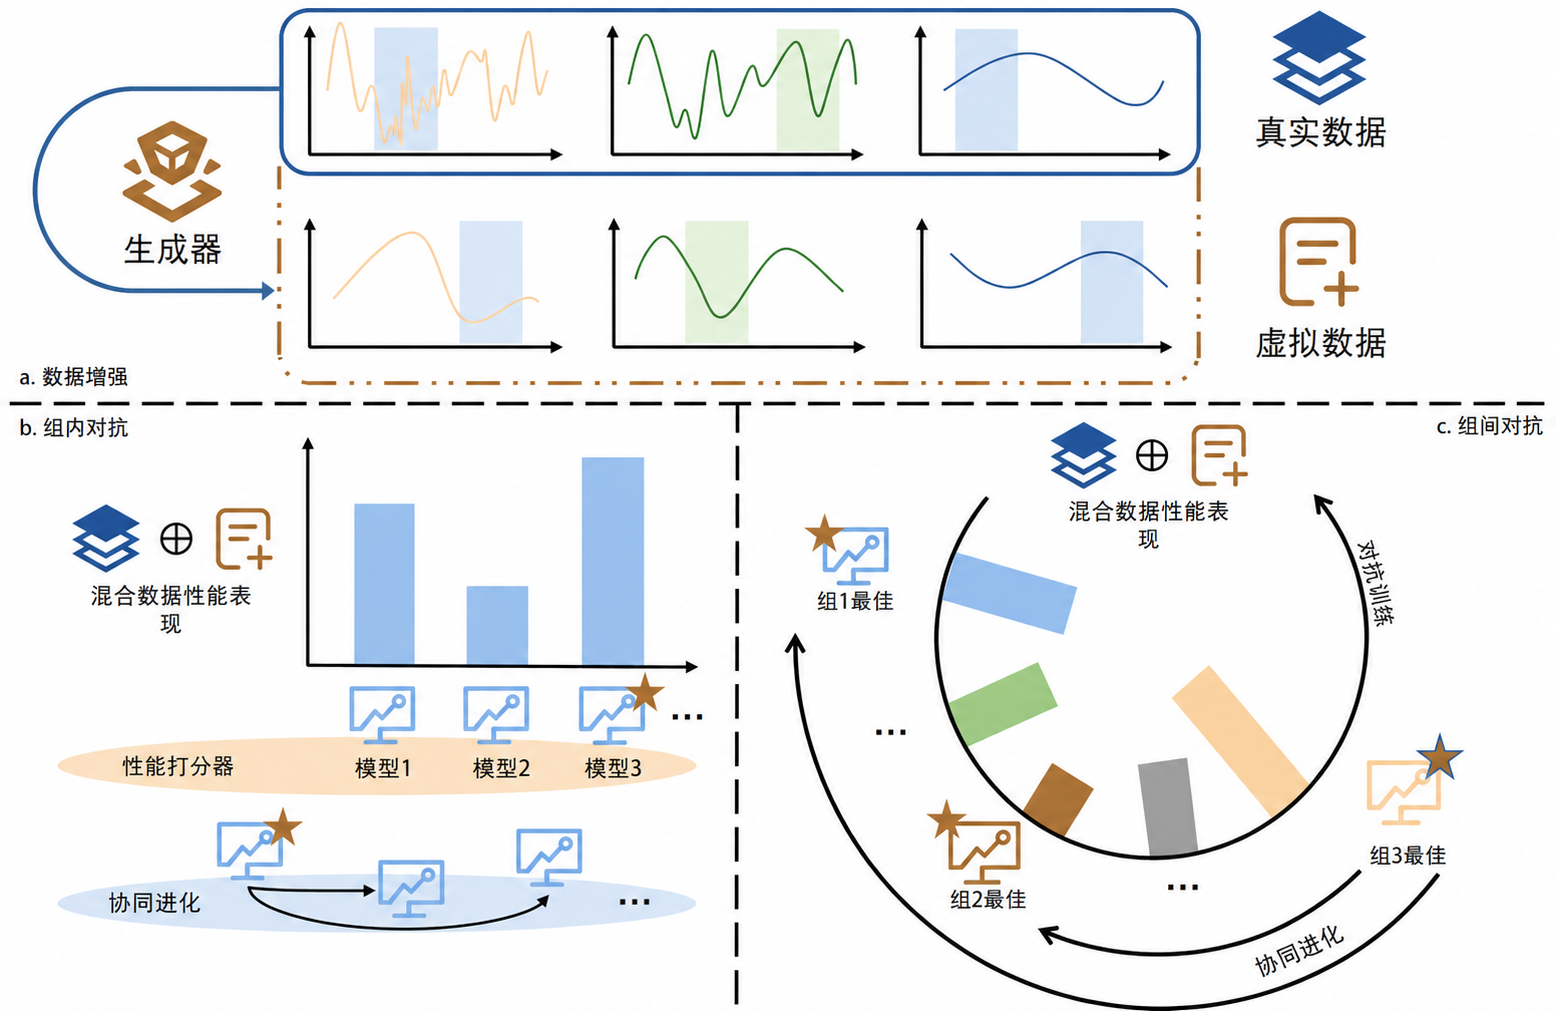
\includegraphics[width=0.85\textwidth]{data/images/highdimframework_cn.png}
\caption{训练策略概览: 监督重构与赛马场训练机制}
% \caption{Overview of Pre-training Strategies: Supervised Reconstruction and 赛马场竞争机制.}

\label{fig:赛马场竞争机制}
\end{figure}


\subsection{过早收敛问题与赛马场竞争机制引入动因}
金融市场数据的高维、高噪与非平稳特征，使得传统时间序列分析难以长期提取稳定表征。在普通训练流程中，模型一旦在某类样本或某组因子上形成早期优势，后续更新往往会继续强化这一优势路径，从而降低对弱幅度但具有解释价值因子的探索能力。本章首先以变分自编码器作为基准表征学习方法，通过压缩与重构学习高维数据中的紧凑表示；在此基础上，引入赛马场竞争机制，将候选模型置于持续评分、竞争、淘汰和迁移的训练过程中。该设计的目的在于，将一次性训练后的静态使用方式转化为动态更新机制，从而缓解高维因子建模中的过早收敛问题。

为检验模型在不同金融任务中的适应性，本章将预测任务划分为三个递进层次。回归任务要求输出连续实数值以逼近未来价格，用于检验模型的精细拟合能力；分类任务关注价格变动方向，用于评估模型对基本方向信息的识别能力；投资任务进一步将未来收益率划分为下跌、平稳和上涨三个区间，使模型输出更接近买入、卖出或观望等交易决策约束。

上述任务组织说明了赛马场竞争机制并非只服务于单一预测目标，而是通过统一的因子表征进入不同层次的金融任务。图~\ref{fig:highdim-task}进一步给出高维金融因子输入、模型组织形式与预测目标之间的对应关系。

\begin{figure}[!htbp]
    \centering 
    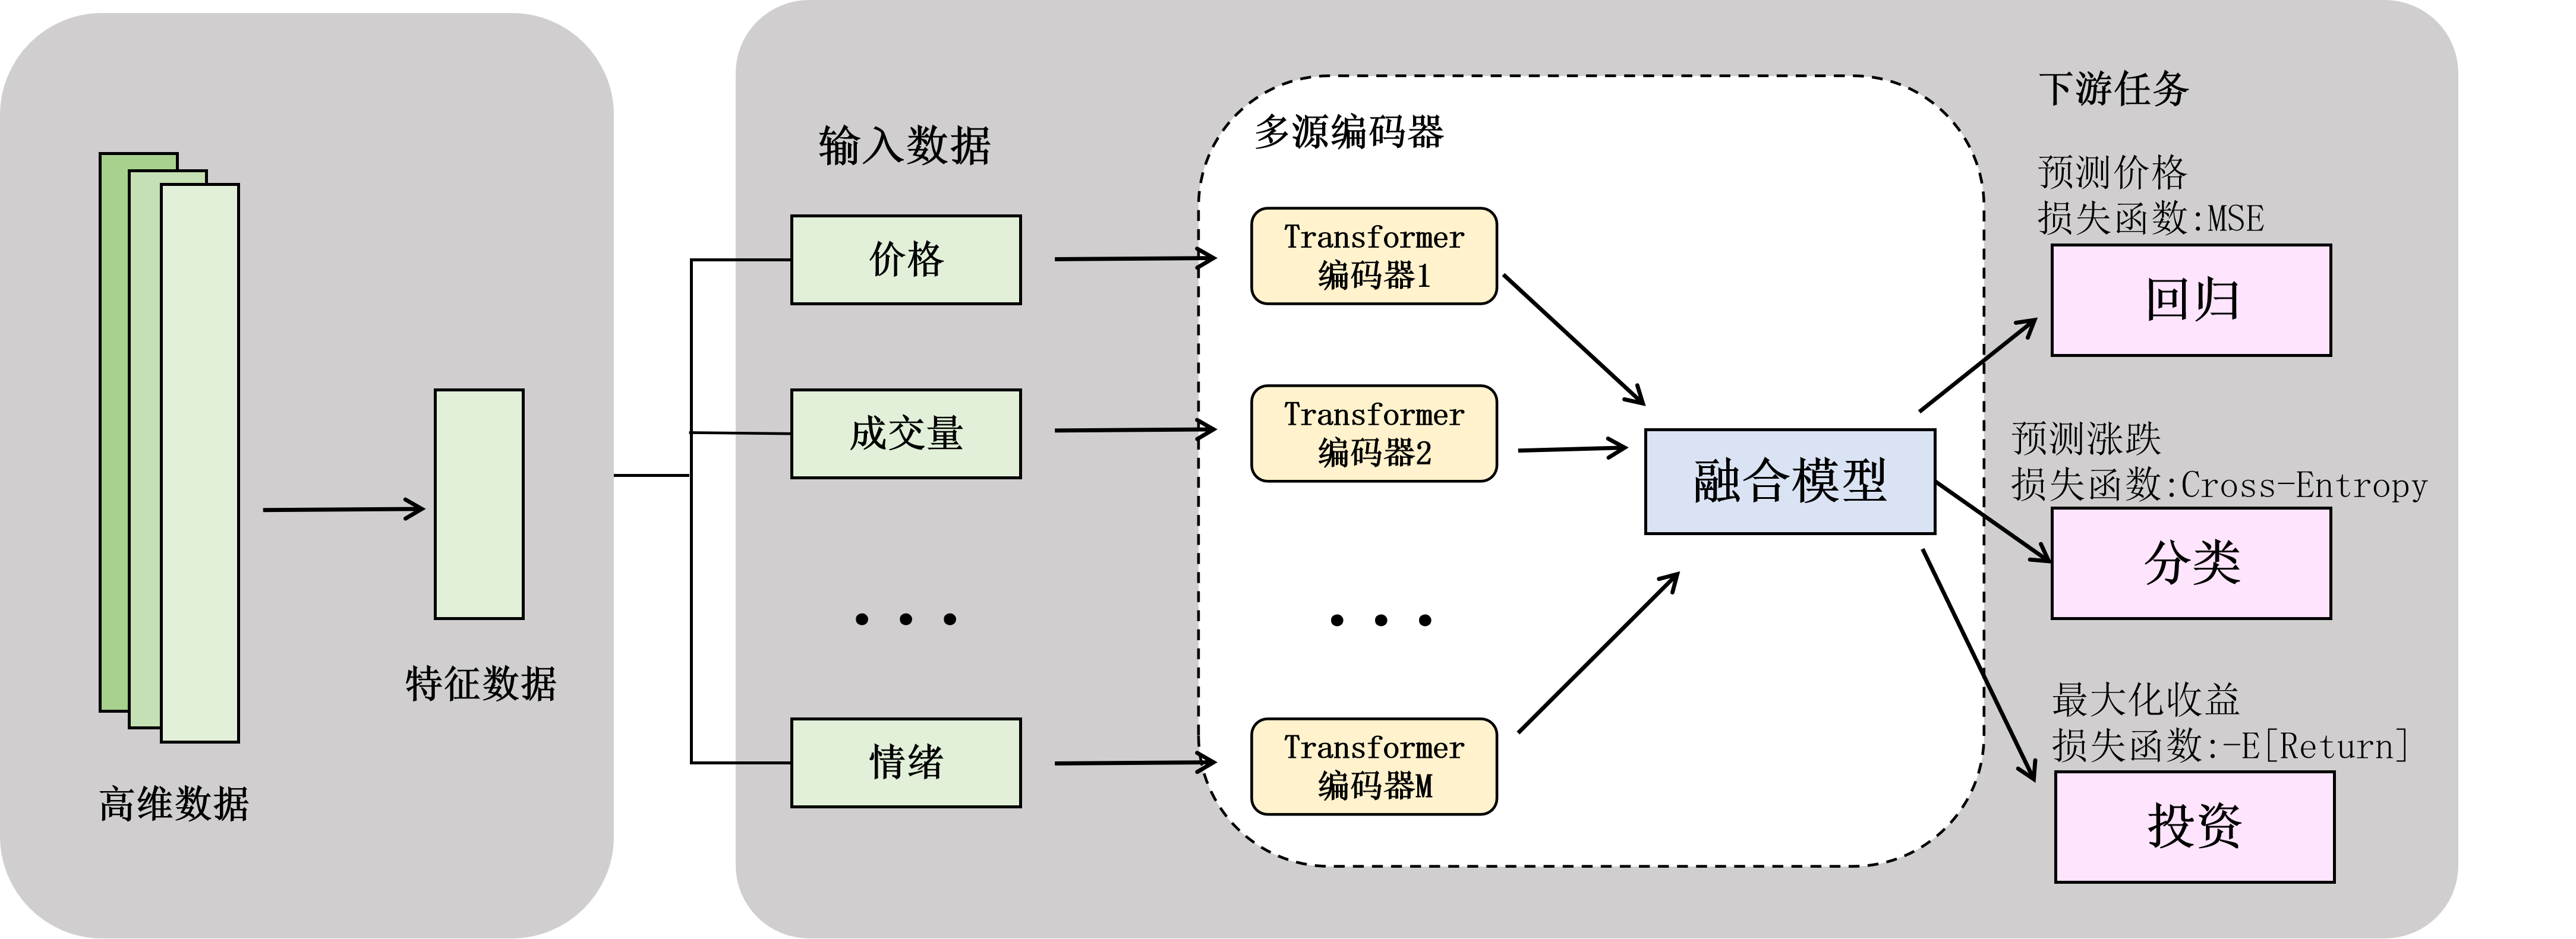
\includegraphics[width=0.8\textwidth]{figures/chap4/高维任务.png} 
    \caption{基于赛马场竞争机制的高维金融因子建模任务}
    \label{fig:highdim-task}
\end{figure}

金融市场数据通常具有高度异构性，不同类型的指标往往反映市场结构的不同侧面，例如基础交易信息刻画流动性与价格行为，技术分析信号揭示趋势与动量，而工程化特征则强调统计结构或潜在风险暴露。图结构半监督学习研究说明，当样本之间存在关系依赖时，显式刻画结构关系有助于提升表示学习效果\cite{kipf2016semi}。这一思想对高维金融因子建模具有启发意义：多源因子并不是简单并列的输入变量，而是可能在资产、时间和市场状态之间形成复杂关联。进一步地，图生成模型研究也表明，复杂结构数据的表示与生成需要同时考虑节点属性和整体结构关系\cite{simonovsky2018graphvae}。因此，在金融因子建模中，若将价量、技术、动量等异构特征直接混合输入同一模型，容易导致特征干扰与表示退化，从而削弱模型对复杂市场动态的刻画能力。

在实际多因子研究中，情绪因子等非价格信息也会被纳入选股与因子组合框架，说明金融特征空间本身具有多源异构属性\cite{ye2023system}。这进一步提示本文，第三章的方法设计不能把所有金融特征视为同质输入，而应先在语义层面区分不同信息来源，再让模型在相对清晰的特征结构上进行竞争和筛选。

基于上述考虑，本章依据语义相关性实施特征分组策略，将输入划分为三个独立组别。第一组为基础价量特征，包括开盘价、最高价、最低价、收盘价和成交量，用于刻画市场运行的基本状态；第二组为技术分析指标，包括移动平均线、平滑异同移动平均线和布林带等，用于描述趋势与波动特征；第三组为动量与随机指标，聚焦相对强弱指数、随机指标等，用于捕捉超买超卖状态及短期反转信号。每一组特征由专用编码器独立处理，以减少不同语义特征之间的相互干扰，并为后续赛马场竞争机制提供更稳定的候选因子表征。

为了消除不同特征量纲之间的差异，我们对每一组特征分别进行了 Z-score 标准化处理。这一步骤保证了每组特征在输入模型时具有相似的分布尺度，从而改善了模型的收敛速度和稳定性。在样本构造方面，我们采用了滑动窗口技术，将时间窗口大小设定为 60 个时间步。这意味着模型将利用过去 60 个交易日的数据来预测未来的市场状态，以覆盖中短期的市场规律。

高维金融数据中充斥着大量噪声，且不同语义类型的特征（如价量、技术指标、动量）在统计性质上存在明显差异。直接在原始空间中进行对抗训练极易导致模式崩溃。为解决这一问题，本阶段引入变分自编码器进行重构预训练，将异构的高维噪声数据映射到一个平滑、连续且去噪的统一潜在空间中，为后续的对抗博弈提供稳定的表征基础。基于不同语义类型的金融特征具有各自独特演化规律的假设，我们构建了一个多编码器融合系统。给定原始输入序列 $X = \{X^{(1)}, X^{(2)}, X^{(3)}\}$，其中 $X^{(k)} \in \mathbb{R}^{B \times T \times D_k}$（$k=1,2,3$）分别对应基础价量特征、技术分析指标与动量随机指标三组特征，$B$ 为批大小，$T$ 为时间步长，$D_k$ 为第 $k$ 组特征维度。

每组特征由独立的 Transformer 编码器 $E^{(k)}_{\phi_k}$ 处理，提取各组的时序表示\cite{vaswani2017attention}：
\begin{equation}
h^{(k)} = E^{(k)}_{\phi_k}(X^{(k)}), \quad h^{(k)} \in \mathbb{R}^{B \times T \times d},
\end{equation}
其中 $d$ 为编码器隐藏维度。随后，三组表示经融合模块 $\mathcal{F}$（注意力机制）整合为统一的潜在表示：
\begin{equation}
h = \mathcal{F}(h^{(1)}, h^{(2)}, h^{(3)}).
\end{equation}

在变分自编码器框架下，融合后的表示经线性映射生成潜变量分布参数：
\begin{equation}
(\mu, \log \sigma^2) = \text{Linear}(h),
\end{equation}
并通过重参数化技巧获得潜变量采样：
\begin{equation}
z = \mu + \sigma \odot \epsilon, \quad \epsilon \sim \mathcal{N}(0, I).
\end{equation}

解码器 $\text{Dec}_{\psi}$ 据此重构原始输入：
\begin{equation}
\hat{X} = \text{Dec}_{\psi}(z).
\end{equation}

训练目标为最大化证据下界，等价于最小化以下损失：
\begin{equation}
\mathcal{L}_{\text{变分自编码器}} = \|X - \hat{X}\|_2^2 + \beta \, D_{\mathrm{KL}}\big(q_\phi(z|X) \,\|\, p(z)\big),
\end{equation}
其中第一项为重构损失，第二项为 库尔贝克—莱布勒散度正则化项，$\beta$ 为平衡系数，$p(z) = \mathcal{N}(0, I)$ 为标准正态先验。库尔贝克—莱布勒散度项迫使后验分布 $q_\phi(z|X)$ 逼近先验分布，使得潜在空间更加平滑连续，避免过拟合并提升泛化能力。

预训练完成后，选择验证集上重构损失最低的模型，保留其编码器 $\{E^{(1)}_{\phi_1}, E^{(2)}_{\phi_2}, E^{(3)}_{\phi_3}, \mathcal{F}\}$ 作为共享表示模块，冻结全部编码器参数，移除解码器。后续所有训练阶段中，输入数据均通过固定编码器映射至潜空间：
\begin{equation}
z = \mathcal{F}\big(E^{(1)}_{\phi_1}(X^{(1)}), E^{(2)}_{\phi_2}(X^{(2)}), E^{(3)}_{\phi_3}(X^{(3)})\big) \in \mathbb{R}^{B \times T \times d_z},
\end{equation}
其中 $d_z$ 为潜在特征维度。对抗训练由此在结构化、去噪的潜空间上进行，而非在高维、噪声充斥的原始特征空间中直接博弈。

经过 $E_{\text{init}}$ 轮独立训练后，所有生成器已具备基本的序列到目标映射能力，为后续对抗训练提供了稳定的初始化基础。

在验证集上对所有生成器和判别器进行全局性能评估，分别识别全局最优与最差的模型：
\begin{equation}
G_{\text{best}} = \arg\min_{G_{i,j} \in \mathcal{G}} \mathcal{L}_{\text{task}}(G_{i,j}), \quad
G_{\text{worst}} = \arg\max_{G_{i,j} \in \mathcal{G}} \mathcal{L}_{\text{task}}(G_{i,j}).
\end{equation}

在完成预训练与对抗式精炼后，模型已能够提取高质量且具备分布感知能力的潜在表示。基于此，我们连接任务特定预测头并进行端到端微调，以适配不同金融应用场景。整体训练流程遵循严格的偏序执行策略：先进行变分自编码器表示学习，再执行赛马场对抗精炼，最后根据任务类型进行下游微调。

\subsection{动态选优规则与模型演化路径}
金融时间序列通常呈现较强的非平稳性与分布漂移特征，直接在高维原始空间中进行对抗训练容易引发收敛不稳定与模式崩溃。本章采用“先表征、后赛马”的多阶段训练方式：先通过变分自编码器重构预训练提取结构化潜在表示，再进行多生成器独立预热以建立基线预测能力，随后在潜在空间中引入群组交叉对抗（GCA）作为辅助的交叉校验环节，最后由赛马场竞争机制实施动态评分、末位淘汰与知识蒸馏。需要强调的是，GCA在本章中并不是主体方法，而是为赛马场竞争提供分布反馈和模型差异校验；本章的核心仍是通过持续竞争和知识迁移抑制过早收敛。该路径旨在使后续竞争过程建立在相对稳定的潜空间之上，降低早期对抗训练直接拟合复杂分布带来的震荡。

为展示高维金融因子建模框架的训练逻辑，本节将上述过程整理为形式化算法流程。整个训练过程按照固定阶段顺序执行：先进行表示学习（变分自编码器预训练），再执行交叉对抗校验与赛马场竞争，最后根据任务类型进行下游微调。

图~\ref{fig:HIGHDIM-workflow}对应展示这一训练流程中的关键步骤，使后续算法描述能够与全局评估、学生模型培养、末位淘汰替换和对齐训练等环节保持对应。

\begin{figure}[!htbp]
    \centering
    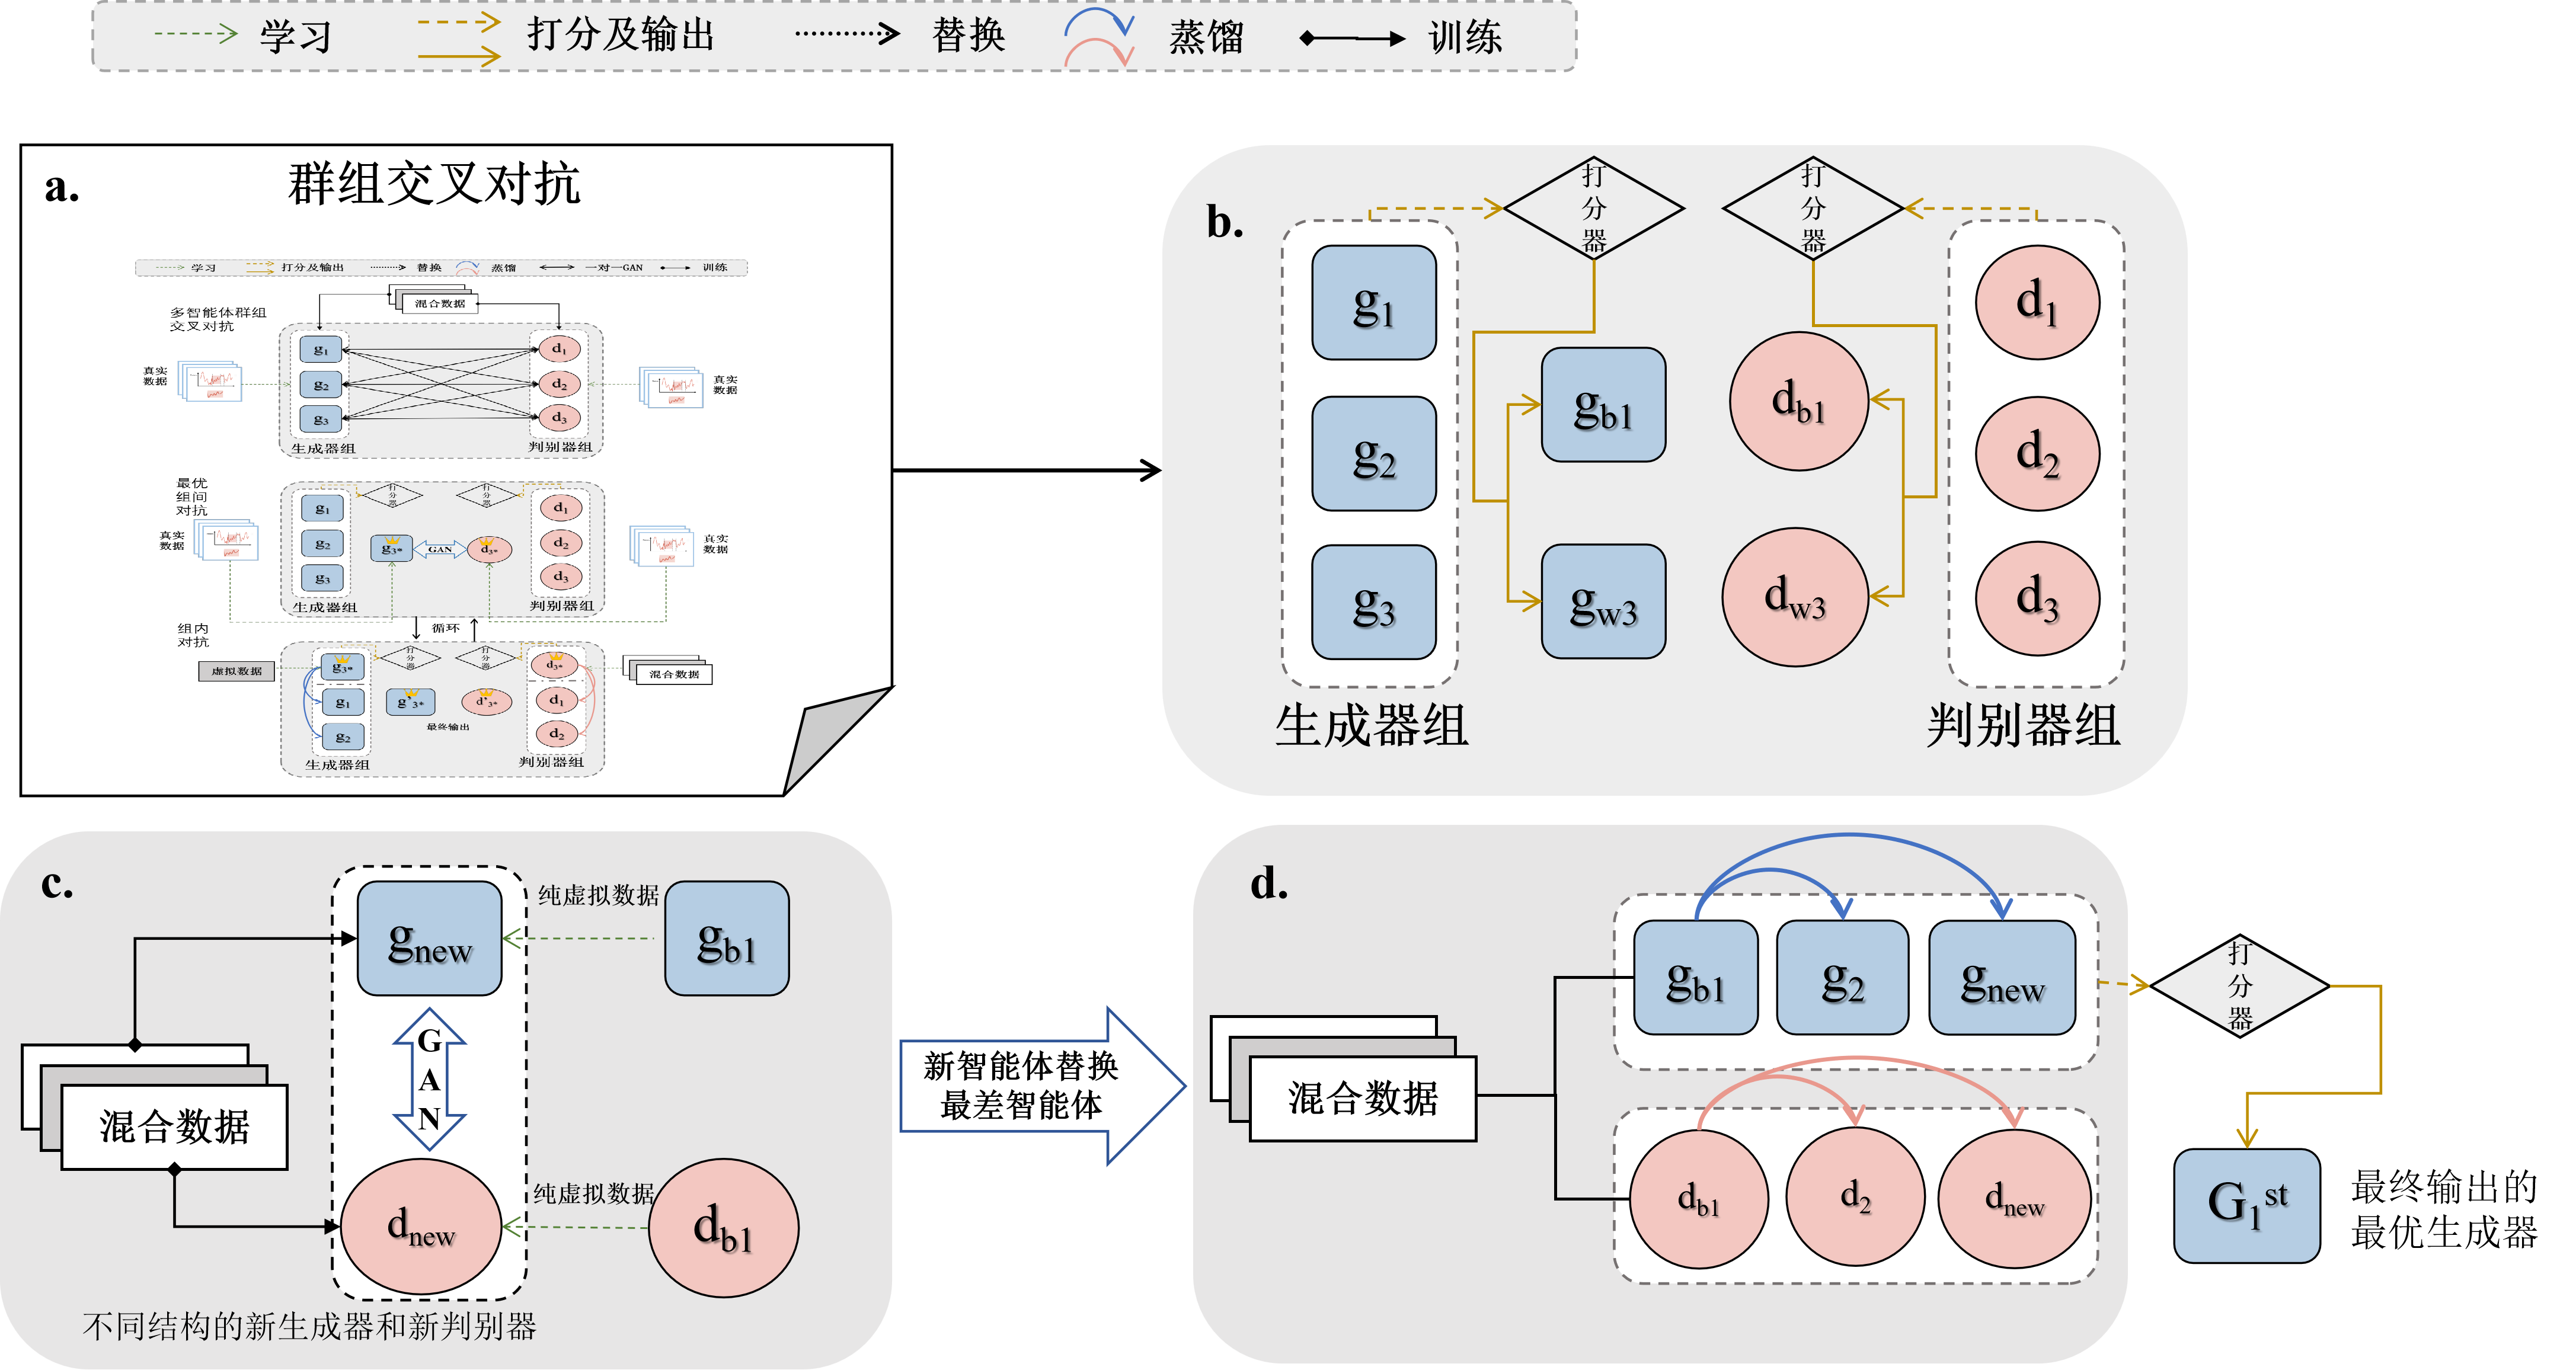
\includegraphics[width=0.8\textwidth]{figures/chap4/赛马场对称.png}
    \caption{赛马场训练流程示意图}
    \label{fig:HIGHDIM-workflow}
\end{figure}

\begin{algorithm}[H]
\caption{高维因子建模框架总体训练流程}
\label{alg:highdim_overall}
\begin{algorithmic}[0]
\Require 原始特征序列 $X \in \mathbb{R}^{T \times D_{\text{raw}}}$，特征分组列表 $\mathcal{F}_1, \ldots, \mathcal{F}_K$；超参数：$N_{\text{VAE}}$（变分自编码器预训练轮数），$N_{\text{GCA}}$（对抗训练轮数），$N_{\text{RT}}$（赛马场竞争机制训练轮数），$\lambda_{\text{adv}}$（对抗权重），$\delta$（投资阈值），$\lambda$（误差罚项）
\Ensure 训练好的生成器 $G^{\star}$，最优判别器 $D^{\star}$，各任务的预测头 $\phi_{\text{reg}}, \phi_{\text{cls}}, \phi_{\text{inv}}$
\Statex
\State \textbf{/* 阶段 1：变分自编码器表示预训练 */}
\State $Z \leftarrow \text{变分自编码器预训练}(X; \theta_E, \theta_D)$ \Comment{学习潜在表示 $Z \in \mathbb{R}^{T \times d_{\text{model}}}$}
\State $E \leftarrow \text{Freeze}(E)$ \Comment{冻结编码器，用于下游特征提取}
\Statex
\State \textbf{/* 阶段 2：交叉对抗校验与赛马场竞争 */}
\State 初始化生成器组 $\mathcal{G} = \{G_1, \ldots, G_N\}$ 和判别器组 $\mathcal{D} = \{D_1, \ldots, D_M\}$
\State $\mathcal{G}, \mathcal{D} \leftarrow \text{执行赛马场竞争机制}(\mathcal{G}, \mathcal{D}, Z)$ \Comment{见算法 \ref{alg:highdim_mgca_detail}}
\Statex
\State \textbf{/* 阶段 3：下游任务微调 */}
\State 连接任务特定预测头：$\phi_{\text{reg}}$（回归头），$\phi_{\text{cls}}$（分类头），$\phi_{\text{inv}}$（投资头）
\State 在 $Z$ 上分别微调各预测头，最小化对应任务损失
\Statex
\State \Return $\mathcal{G}, \mathcal{D}, \phi_{\text{reg}}, \phi_{\text{cls}}, \phi_{\text{inv}}$
\end{algorithmic}
\end{algorithm}

\begin{algorithm}[H]
\caption{赛马场竞争与交叉校验详细流程}
\label{alg:highdim_mgca_detail}
\begin{algorithmic}[0]
\Require 潜在表示序列 $Z \in \mathbb{R}^{T \times d_{\text{model}}}$，混合比例 $1-\alpha$（真实数据），生成器组 $\mathcal{G}$，判别器组 $\mathcal{D}$，打分阈值 $\theta_{\text{score}}$
\Ensure 最优生成器 $G^{\star}$，最优判别器 $D^{\star}$
\Statex
\State \textbf{/* Stage 1：生成器预训练 */}
\For{轮次 $\in \{1, \ldots, N_{\text{VAE}}\}$}
    \State $\mathcal{L}_{\text{VAE}} \leftarrow \text{ELBO}(G_{\text{VAE}}(x), x)$
    \State 使用 $\mathcal{L}_{\text{VAE}}$ 更新 $G_{\text{VAE}}$ 和 $E$
\EndFor
\Statex
\State \textbf{/* Stage 2：混合数据生成 */}
\State $\tilde{Z} \leftarrow G_{\text{VAE}}(Z)$ \Comment{生成器输出虚拟潜在序列}
\State $Z_{\text{mixed}} \leftarrow \alpha \cdot Z \oplus (1-\alpha) \cdot \tilde{Z}$ \Comment{按比例混合}
\Statex
\State \textbf{/* Stage 3：组内对抗与蒸馏 */}
\For{每组判别器 $\mathcal{D}^{(g)}$}
    \State 在 $Z_{\text{mixed}}$ 上并行训练组内所有判别器
    \State 在 $\mathcal{D}_{\text{val}}$ 上评估，选出组内最优 $D_g^{\star}$（交叉熵最小）
    \For{组内每个判别器 $D_k \neq D_g^{\star}$}
        \State $\mathcal{L}_{\text{distill}} \leftarrow \text{MSE}(\text{Feat}_{D_k}, \text{Feat}_{D_g^{\star}}) + \text{MSE}(\text{Logits}_{D_k}, \text{Logits}_{D_g^{\star}})$
        \State 使用 $\mathcal{L}_{\text{distill}}$ 更新 $D_k$
    \EndFor
\EndFor
\Statex
\State \textbf{/* Stage 4：组间蒸馏与新学生竞争 */}
\State 从所有 $D_g^{\star}$ 中选出全局最优 $D^{\star}$ 和最差 $D^{\dagger}$
\State 实例化新学生判别器：$D_{\text{new}} \leftarrow \text{DeepCopy}(D^{\star})$
\State 在 $Z_{\text{mixed}}$ 上训练 $D_{\text{new}}$：蒸馏所有判别器的平均表现
\State $D^{\dagger} \leftarrow D_{\text{new}}$ \Comment{替换最差判别器}
\Statex
\State \Return $G_{\text{VAE}},\; D^{\star}$
\end{algorithmic}
\end{algorithm}

\begin{algorithm}[H]
\caption{下游任务推理与信号生成}
\label{alg:highdim_inference}
\begin{algorithmic}[0]
\Require 当前时刻特征窗口 $x_t \in \mathbb{R}^{W \times D_{\text{raw}}}$，训练好的生成器 $G^{\star}$，变分自编码器编码器 $E$，各任务预测头 $\phi_{\text{reg}}, \phi_{\text{cls}}, \phi_{\text{inv}}$，置信度阈值 $c_{\min}$
\Ensure 交易信号 $a_t \in \{-1, 0, +1\}$，动态权重 $w_t$
\Statex
\State \textbf{/* 步骤 1：潜在表示提取 */}
\State $z_t \leftarrow E(x_t) \in \mathbb{R}^{d_{\text{model}}}$
\Statex
\State \textbf{/* 步骤 2：回归预测 */}
\State $\hat{r}_t^{\text{reg}} \leftarrow \phi_{\text{reg}}(G^{\star}(z_t))$
\Statex
\State \textbf{/* 步骤 3：分类预测 */}
\State $\hat{y}_t^{\text{cls}} \leftarrow \phi_{\text{cls}}(G^{\star}(z_t)) \in \{0, 1, 2\}$ \Comment{下跌/中性/上涨}
\Statex
\State \textbf{/* 步骤 4：投资决策（若启用） */}
\State $a_t^{\text{inv}} \leftarrow \phi_{\text{inv}}(G^{\star}(z_t)) \in \{0, 1, 2\}$
\Statex
\State \textbf{/* 步骤 5：多资产动态权重（回归任务） */}
\State $c_t \leftarrow \text{置信度}(G^{\star}(z_t))$ \Comment{softmax 输出的最大概率}
\State $R_t \leftarrow \sum_{\tau=1}^{t} \hat{r}_{\tau}^{\text{reg}}$ \Comment{累积预测收益率}
\State $S_t \leftarrow \dfrac{(2.5 \cdot c_t - 1) \cdot R_t}{1 + \lambda \cdot \text{MSE}_{\text{val}}}$
\State $w_i \leftarrow \dfrac{|S_i|}{\sum_j |S_j|}$ \Comment{绝对值归一化权重}
\State $L_i \leftarrow \dfrac{\text{TotalEquity} \cdot |w_i|}{P_i \cdot \text{Mult}_i \cdot \text{Margin}_i}$ \Comment{保证金手数}
\Statex
\State \Return $(a_t^{\text{cls}}, a_t^{\text{inv}}), \; S_t, \; L_i$
\end{algorithmic}
\end{algorithm}

传统的单一生成器—判别器架构在面对非平稳金融时间序列时，往往只能拟合局部数据分布。为避免候选模型在进入赛马场竞争之前已经形成过强的单一路径依赖，本框架在预热之后引入群组交叉对抗（GCA）作为辅助校验阶段。该机制通过一对多、组内与组间的交互训练，使不同架构的生成器在相互约束中形成差异化预测策略。同时构建 $N_D$ 组条件判别器 $\mathcal{D} = \{D_{k,l}\}$，与生成器群体进行多轮对抗训练：一方面扩展判别反馈来源，另一方面在组内进行性能评估与知识蒸馏，使落后成员向优势成员对齐。经过这一阶段后，生成器与判别器形成相对稳定的交互关系，为后续赛马场竞争机制中的动态淘汰与演化更新提供基础。

在群组交叉对抗完成后，模型群体只获得了初步的分布校验和差异化约束，并不意味着因子表征已经完成动态筛选。本框架进一步引入赛马场竞争机制进行动态淘汰与精炼。即使模型群体保持一定多样性，长时间静态训练后仍可能集中到单一优势路径，导致面对新市场状态时泛化能力下降。赛马场竞争机制通过周期性的全局评估、学生模型培养与末位淘汰替换，引入新的参数起点并淘汰表现不足的成员，使模型群体在持续更新中保持探索能力。由此，GCA承担前置交叉校验功能，赛马场竞争机制承担持续选优、替换和知识迁移功能，二者在训练流程中形成前后衔接而非并列替代关系。

创建全新初始化的学生生成器 $G_s$ 与学生判别器 $D_s$，通过交替执行对抗训练与知识蒸馏进行培养。学生判别器向全局最优判别器 $D_{\text{best}}$ 学习，蒸馏损失涵盖 logits 对齐、概率分布对齐与中间层特征对齐三个层面：
\begin{equation}
\mathcal{L}_{D_s}^{\text{distill}} = \lambda_{\text{feat}}\big(\|o_s - o_t\|_2^2 + \|\sigma(o_s) - \sigma(o_t)\|_2^2 + \|f_s - f_t\|_2^2\big).
\end{equation}
学生生成器向全局最优生成器 $G_{\text{best}}$ 学习，总损失结合蒸馏、对抗与重构三项：
\begin{equation}
\mathcal{L}_{G_s}^{\text{distill}} = \lambda_d \cdot \|G_s(z) - G_{\text{best}}(z)\|_2^2 + \lambda_{\text{adv}} \cdot \ell_{\text{二元交叉熵}}(D_s(z, G_s(z)), \mathbf{1}) + \mathcal{L}_{\text{task}}(G_s(z), y).
\end{equation}


训练完成后，执行末位淘汰替换：$G_{\text{worst}} \leftarrow G_s,\; D_{\text{worst}} \leftarrow D_s$，同时重置被替换位置的优化器状态。替换完成后，所有生成器—判别器对进入局部对抗校验训练，并同时通过蒸馏损失向全局最优生成器 $G_{\text{best}}$ 的输出对齐：
\begin{equation}
\mathcal{L}_{G_{i,j}}^{\text{align}} = \mathcal{L}_{\text{task}}(\hat{y}_{i,j}, y) + \lambda_{\text{adv}} \cdot \mathcal{L}_{\text{adv}}^{(i,j)} + \lambda_d \cdot \|\hat{y}_{i,j} - G_{\text{best}}(z)\|_2^2.
\end{equation}
赛马场竞争机制通过“评估—培养—淘汰—对齐”的循环过程，使模型群体在竞争筛选与协作蒸馏中持续调整，其效果主要体现在非平稳数据下的泛化表现和训练稳定性上。

动态选优规则主要解决“谁更适合当前市场状态”的评价问题；若缺少跨阶段知识继承和反向校正，模型群体仍可能在若干轮筛选后集中到单一优势路径。因此，后续的成熟—新生模型双向知识迁移机制，是赛马场竞争机制能够持续演化而不退化为静态集成的关键环节。

本章的损失函数设计主要包含任务损失、对抗损失与蒸馏损失三类，分别对应不同任务的特性和对抗训练的需求。对于回归任务，我们设计了金融感知重构损失，对开盘价、最高价、最低价、收盘价与成交量五个核心维度赋予特定权重：
\begin{equation}
\mathcal{L}_{\text{financial}} = w_{\text{price}} \cdot \frac{1}{4} \sum_{k \in \{O,H,L,C\}} \text{均方误差}(y_k, \hat{y}_k) + w_{\text{vol}} \cdot \text{均方误差}(y_V, \hat{y}_V)
\end{equation}
其中 $w_{\text{price}}$ 和 $w_{\text{vol}}$ 分别为价格类特征和成交量特征的权重（默认分别设为1.0和0.8）。对于分类任务，使用标准交叉熵损失；对于投资任务，采用严格的阈值法生成真实标签 $y_{\text{inv}}$，设定阈值 $\delta$（默认0.02），将连续收益率映射为做空/持有/做多三类决策，同样使用交叉熵损失优化。对抗损失定义为生成样本在判别器眼中的二元交叉熵损失，蒸馏损失通过均方误差衡量学生模型与最优教师模型输出之间的差异，实现跨代知识传递。

\subsection{模型预热与公平竞争约束}
在完成变分自编码器重构预训练、获得结构化潜在表示后，本框架进一步对多个生成器进行独立预热，以消除对抗训练初期的“冷启动”问题。
在对抗训练的早期阶段，如果生成器和判别器均从零开始随机初始化，极易陷入梯度震荡或导致生成器被判别器迅速压制，从而丧失探索能力。本阶段实施多生成器独立预热机制，在不引入对抗信号的情况下，仅通过任务损失为所有生成器建立基本的序列到目标映射能力，确保它们在进入后续对抗训练前具备合格的基线预测水平。我们构建 $N_G$ 组生成器，每组包含 $P$ 个成员，记为 $\mathcal{G} = \{G_{i,j}\}_{i=1,\ldots,N_G;\, j=1,\ldots,P}$。为保障架构多样性，组内成员采用异构网络结构（门控循环单元、长短期记忆网络、Transformer架构 交替分配），使不同生成器能够从不同的归纳偏置出发探索数据分布。

每个生成器接受潜在特征 $z$ 作为输入，输出预测值 $\hat{y}_{i,j} = G_{i,j}(z)$。预热阶段仅使用任务损失进行独立训练，不引入对抗信号：
\begin{equation}
\mathcal{L}_{\text{pretrain}}^{(i,j)} = \mathcal{L}_{\text{task}}(\hat{y}_{i,j},\, y),
\end{equation}
其中 $\mathcal{L}_{\text{task}}$ 根据任务类型定义：回归任务使用均方误差，分类与投资任务使用交叉熵损失。对于回归任务，当目标列包含开盘价、最高价、最低价、收盘价与成交量五个维度时，进一步采用金融感知重构损失，对价格维度和成交量维度分别赋予不同权重。

公平竞争约束为后续知识迁移提供了统一的评价基础。只有在所有候选模型按照相同任务损失、相同验证规则和相同对抗约束进行比较时，成熟模型的经验边界与新生模型的差异化反馈才具有可比性。由此，动态选优规则、公平竞争约束与双向知识迁移共同构成赛马场竞争机制的主要训练环节。

\subsection{成熟—新生模型的双向知识迁移机制}
在赛马场竞争机制中，成熟模型与新生模型不只是替换关系，而是动态演化过程中的两类功能角色。成熟模型指在当前评分规则下已经获得相对稳定表现的候选模型，其优势在于能够提供较高质量的特征表达和预测基准；新生模型则指在训练过程中被重新初始化或引入的候选模型，其作用在于为模型群体提供新的参数起点、结构扰动和探索方向。若只保留成熟模型，系统容易沿已有优势路径过早收敛；若只依赖新生模型，训练过程又会缺乏稳定的知识继承。因此，本章将二者之间的关系设计为双向知识迁移过程，以在稳定性与探索性之间取得平衡。

成熟模型向新生模型的知识迁移主要用于降低新生模型的冷启动成本。在动态选优规则确定当前优势模型后，系统可将成熟模型的输出分布、特征表示或任务损失方向作为软约束，引导新生模型在训练初期快速接近有效解空间。该过程并不要求新生模型完全复制成熟模型，而是利用成熟模型提供的经验边界，使新生模型在保持结构差异的同时避免无效搜索，从而提高因子建模阶段的训练效率。

新生模型向成熟模型的反向迁移则用于抑制成熟模型的路径固化。当新生模型在某些局部市场状态、特定因子组合或异常波动区间中表现出更优的适应性时，其输出差异不应被简单视为噪声，而应被纳入成熟模型的校正信息。通过将新生模型的有效偏差信号反馈给成熟模型，系统能够迫使成熟模型重新审视已形成的特征依赖关系，降低其对单一优势因子或历史局部模式的过度依赖。

由此，成熟—新生模型的双向知识迁移机制形成了“稳定继承—差异探索—反向校正”的循环过程。成熟模型保证群体演化不偏离已有高性能区域，新生模型维持模型空间的探索能力，二者在统一评分规则和公平竞争约束下共同作用，使赛马场竞争机制不仅能够完成优胜劣汰，还能够延迟单一模型的过早收敛，提升高维金融因子表示在非平稳市场环境下的鲁棒性。

\section{实验}

\subsection{实验数据集}
为检验赛马场竞争方法在高维金融因子建模任务中的表现，本章构建了覆盖多品种、多任务的实验基准。该平台涵盖4大板块（农业、能源、金属、化工）、16种期货品种（棉花、豆粕、玉米、白糖、动力煤、原油、甲醇、焦炭、铜、黄金、热卷、铁矿石、螺纹钢、PP、PTA、PVC），涉及回归、分类和投资三种下游任务范式。实验同时在单资产和多资产组合两个维度上进行验证，共构建10个资产组别（见表\ref{tab:highdimassetGrouping}），以覆盖单一品种、板块内组合、跨板块组合和全市场组合等不同因子结构。所有实验均基于200万元初始资本，回测时间跨度覆盖超过500个交易日。

本章实验不仅比较策略收益高低，也检验赛马场竞争方法是否能够在不同资产、任务和市场状态下改善高维金融因子表征的稳定性、有效性和样本外适应能力。因此，后续分析同时关注收益率、最大回撤、训练误差、分类准确率和跨组一致性等指标，以观察动态选优、末位淘汰与知识迁移对高维因子建模过程的影响。

\begin{table}[!htbp]
\centering
\caption{资产分组配置详情}
\label{tab:highdimassetGrouping}
\small
\setlength{\tabcolsep}{4pt}
\renewcommand{\arraystretch}{1.15}
\begin{tabular}{>{\raggedright\arraybackslash}p{2.4cm} >{\centering\arraybackslash}p{2.4cm} >{\raggedright\arraybackslash}p{7.8cm}}
\toprule
类别 & 资产组别 & 包含资产 \\
\midrule
农业 & 板块组 & 玉米、豆粕、棉花、白糖 \\
\addlinespace
能源 & 板块组 & 原油、动力煤、甲醇 \\
\addlinespace
金属 & 板块组 & 铜、黄金、铁矿石、焦炭、热卷、螺纹钢 \\
\addlinespace
化工 & 板块组 & PTA、PP、PVC \\
\addlinespace
跨板块 & 跨板块小组合 & 铜、黄金、原油 \\
\addlinespace
跨板块 & 跨板块大组合 & 铜、黄金、原油、玉米、豆粕、棉花 \\
\addlinespace
全市场 & 全品种组合 & 全部16种期货品种 \\
\bottomrule
\end{tabular}
\end{table}

以上资产分组覆盖单一品种、板块组合、跨板块组合与全市场组合，能够用于检验赛马场竞争方法在不同因子结构和市场状态下的适应性。

\subsection{实验设计}
本章采用与赛马场竞争机制完全相同网络架构、但未启用动态竞争机制的标准训练模型作为对照组，并通过基于历史数据的滚动回测流程评估赛马场竞争机制带来的增量作用。实验设计的核心目的，是检验动态选优、末位淘汰和知识迁移是否能够改善高维因子表征，而不是仅比较单一模型在某一指标上的局部优劣。

本章实验采用统一的对照框架，将启用赛马场竞争机制的模型与未启用该机制的基准模型进行比较。两类模型保持相同的特征输入、任务划分、网络骨干和回测区间，差异仅在于是否引入动态选优、末位淘汰、知识蒸馏与成熟—新生模型双向知识迁移。通过这种控制变量方式，可以将性能差异主要归因于赛马场竞争机制本身，而不是数据划分、模型容量或任务定义的变化。

为避免单一指标造成误判，实验从训练阶段和回测阶段两个层面展开。训练阶段主要观察均方误差、分类准确率以及不同资产组之间的表现差异，用于判断赛马场竞争方法是否改善因子表征学习过程；回测阶段则关注收益率、最大回撤和最终净值等指标，用于判断被筛选出的因子表征是否能够转化为更稳健的交易表现。该设计与本章的机制定位保持一致，即从多个维度考察赛马场竞争机制对高维金融因子建模的影响。

\subsection{结果分析与讨论}
本节在前述统一对照框架下，从胜率统计、收益凸性、任务类型差异和典型案例四个层面分析赛马场竞争机制的实验表现。基准模型与赛马场竞争机制采用相同的网络结构，区别在于基准模型不启用动态淘汰与进化精炼机制，而采用标准训练流程。稳健动态资产组合研究表明，在市场状态变化和估计误差同时存在时，模型需要通过稳健约束或动态调整机制降低风险暴露的不稳定性\cite{zhu2007robust}。因此，本节不只比较策略收益率，也同时观察最大回撤、夏普比率（Sharpe Ratio）和卡玛比率（Calmar Ratio）等风险调整指标，以判断赛马场竞争机制是否真正改善了高维金融因子建模质量。

在结果解释上，本章避免仅以单个收益指标判断模型优劣。若动态淘汰和知识迁移能够在部分市场中降低回撤、减少极端误判或改善亏损状态，可以说明该机制在高维金融因子建模中具有一定的优化价值；若在部分板块中出现收益下降，也应被理解为机制适用边界的体现，不能简单视为整体失效。基于这一口径，后文依次从整体胜率、收益凸性、任务类型差异和典型品种表现展开分析。

首先，从收益分布和任务差异看，赛马场竞争机制并不是在所有场景中均匀提高收益，而是在部分市场状态下形成较强的上行弹性。获胜案例的平均改进幅度（+98.7％）在绝对值上明显高于败北案例的平均降幅（-62.3％），凸性比率达1.58。在赛马场竞争机制获胜的18个案例中，有7个属于“亏损转盈利”场景，即基准模型产生亏损而赛马场竞争机制实现盈利。以200万元初始资本为基准，Top 10盈利案例合计贡献了超过+630万元的超额利润，其中棉花回归任务单项即贡献了+255.5万元的超额利润。

为了观察超额利润的来源分布，图~\ref{fig:highdimprofitwaterfall}将Top 10盈利案例与Top 5亏损案例的绝对利润影响放在同一尺度下比较。该图主要用于判断正向案例的利润贡献是否能够覆盖负向案例带来的损失，而不是简单展示单个案例的收益高低。
进一步看，图~\ref{fig:highdimtopimprovements}列出了Alpha生成最佳案例（Top 10）。这些案例用于补充说明：赛马场竞争机制的优势并不平均分布于所有资产，而是在部分高维因子关系更易被动态筛选的市场状态中集中体现，其中棉花以340\%的提升幅度位居榜首。

\begin{figure}[!htbp]
    \centering 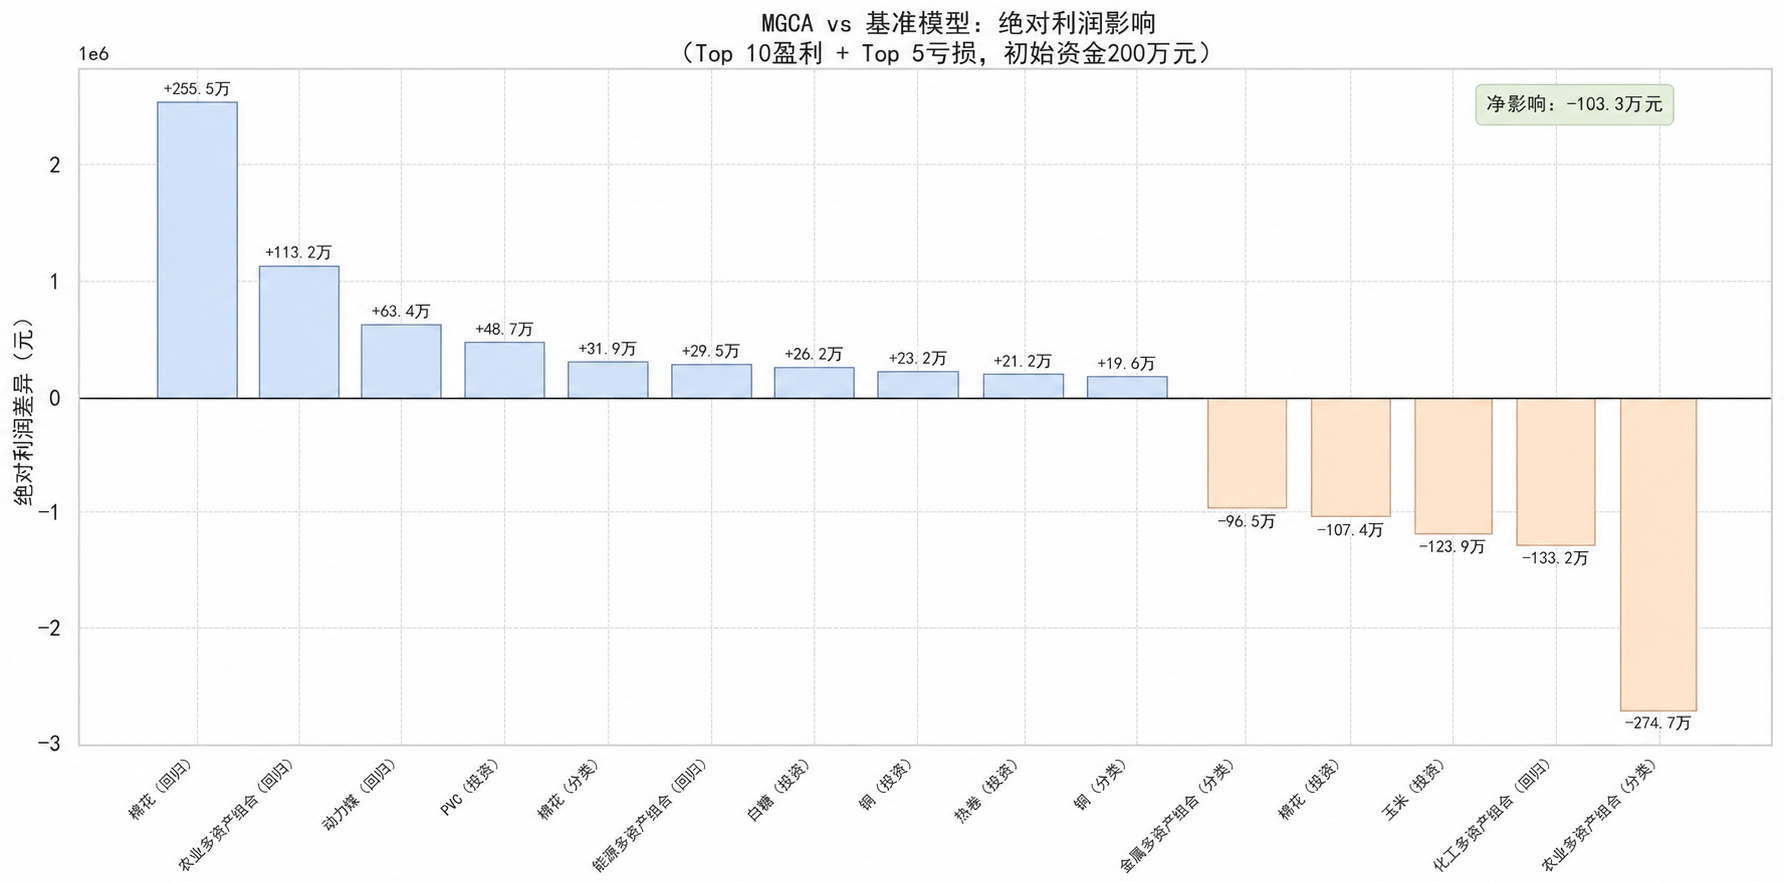
\includegraphics[width=0.8\textwidth]{figures/chap4/fig19_profit_waterfall_cn.png} 
    \caption{绝对利润影响瀑布图（Top 10盈利案例与Top 5亏损案例）}
    \label{fig:highdimprofitwaterfall}
\end{figure}



\begin{figure}[!htbp]
    \centering 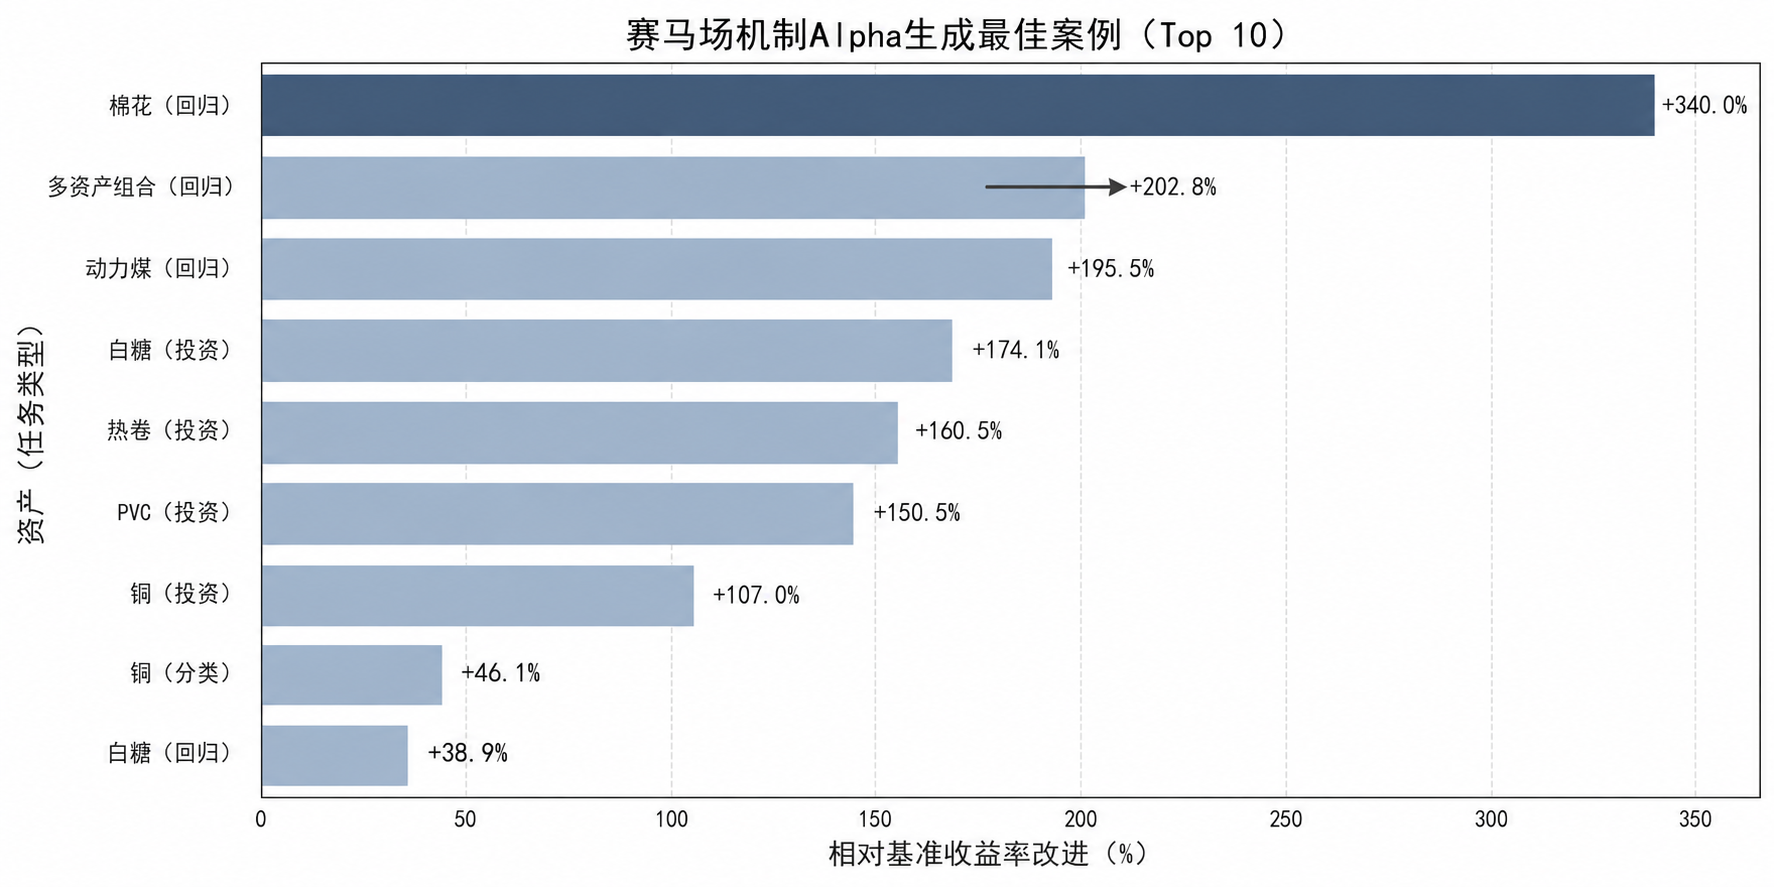
\includegraphics[width=0.8\textwidth]{figures/chap4/fig3_top_improvements_cn.png} 
    \caption{Alpha生成最佳案例（Top 10）}
    \label{fig:highdimtopimprovements}
\end{figure}

从收益改进分布看，图~\ref{fig:highdimreturnDistribution}呈现出明显的右偏长尾特征，尾部包含棉花（+340\%）、能源多资产（+202\%）等正向案例。这说明赛马场竞争机制并非简单提高所有样本的平均表现，而是在部分市场状态下捕捉到收益改善机会。

\begin{figure}[!htbp]
    \centering 
    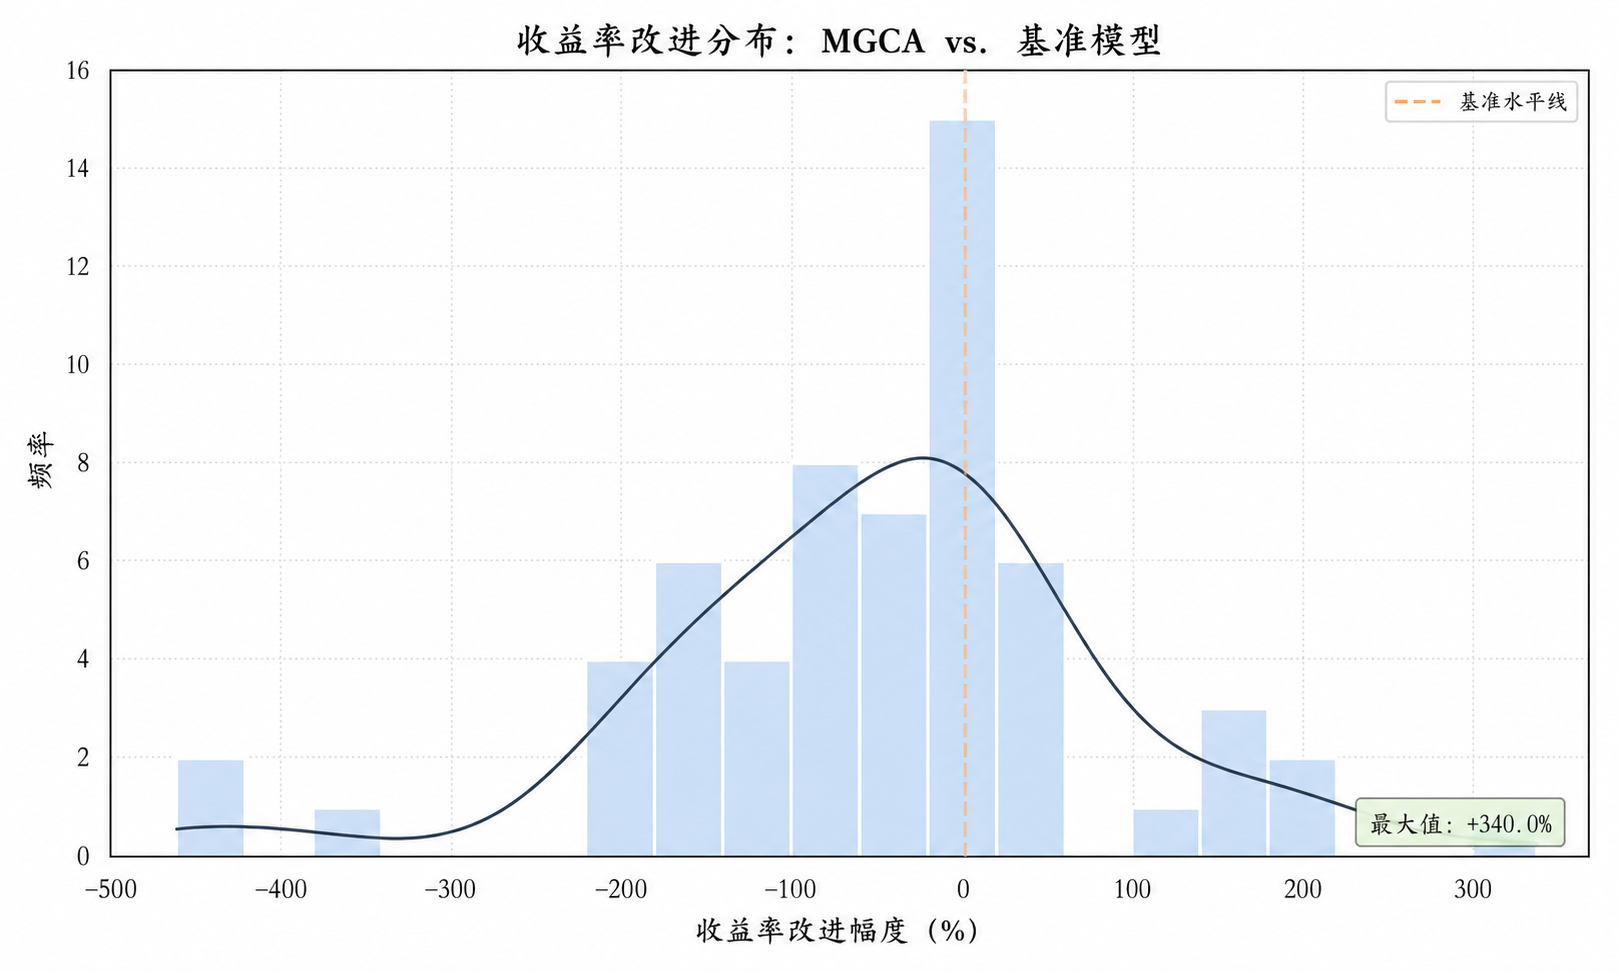
\includegraphics[width=0.8\textwidth]{figures/chap4/fig1_return_distribution_cn.png} 
    \caption{收益率改进分布直方图}
    \label{fig:highdimreturnDistribution}
\end{figure}

任务类型差异进一步说明了该机制的适用场景。图~\ref{fig:highdimtaskcomp}比较了不同任务类型下的平均收益改进幅度，用于判断赛马场竞争机制更容易在哪类预测目标中发挥作用。

\begin{figure}[!htbp]
    \centering 
    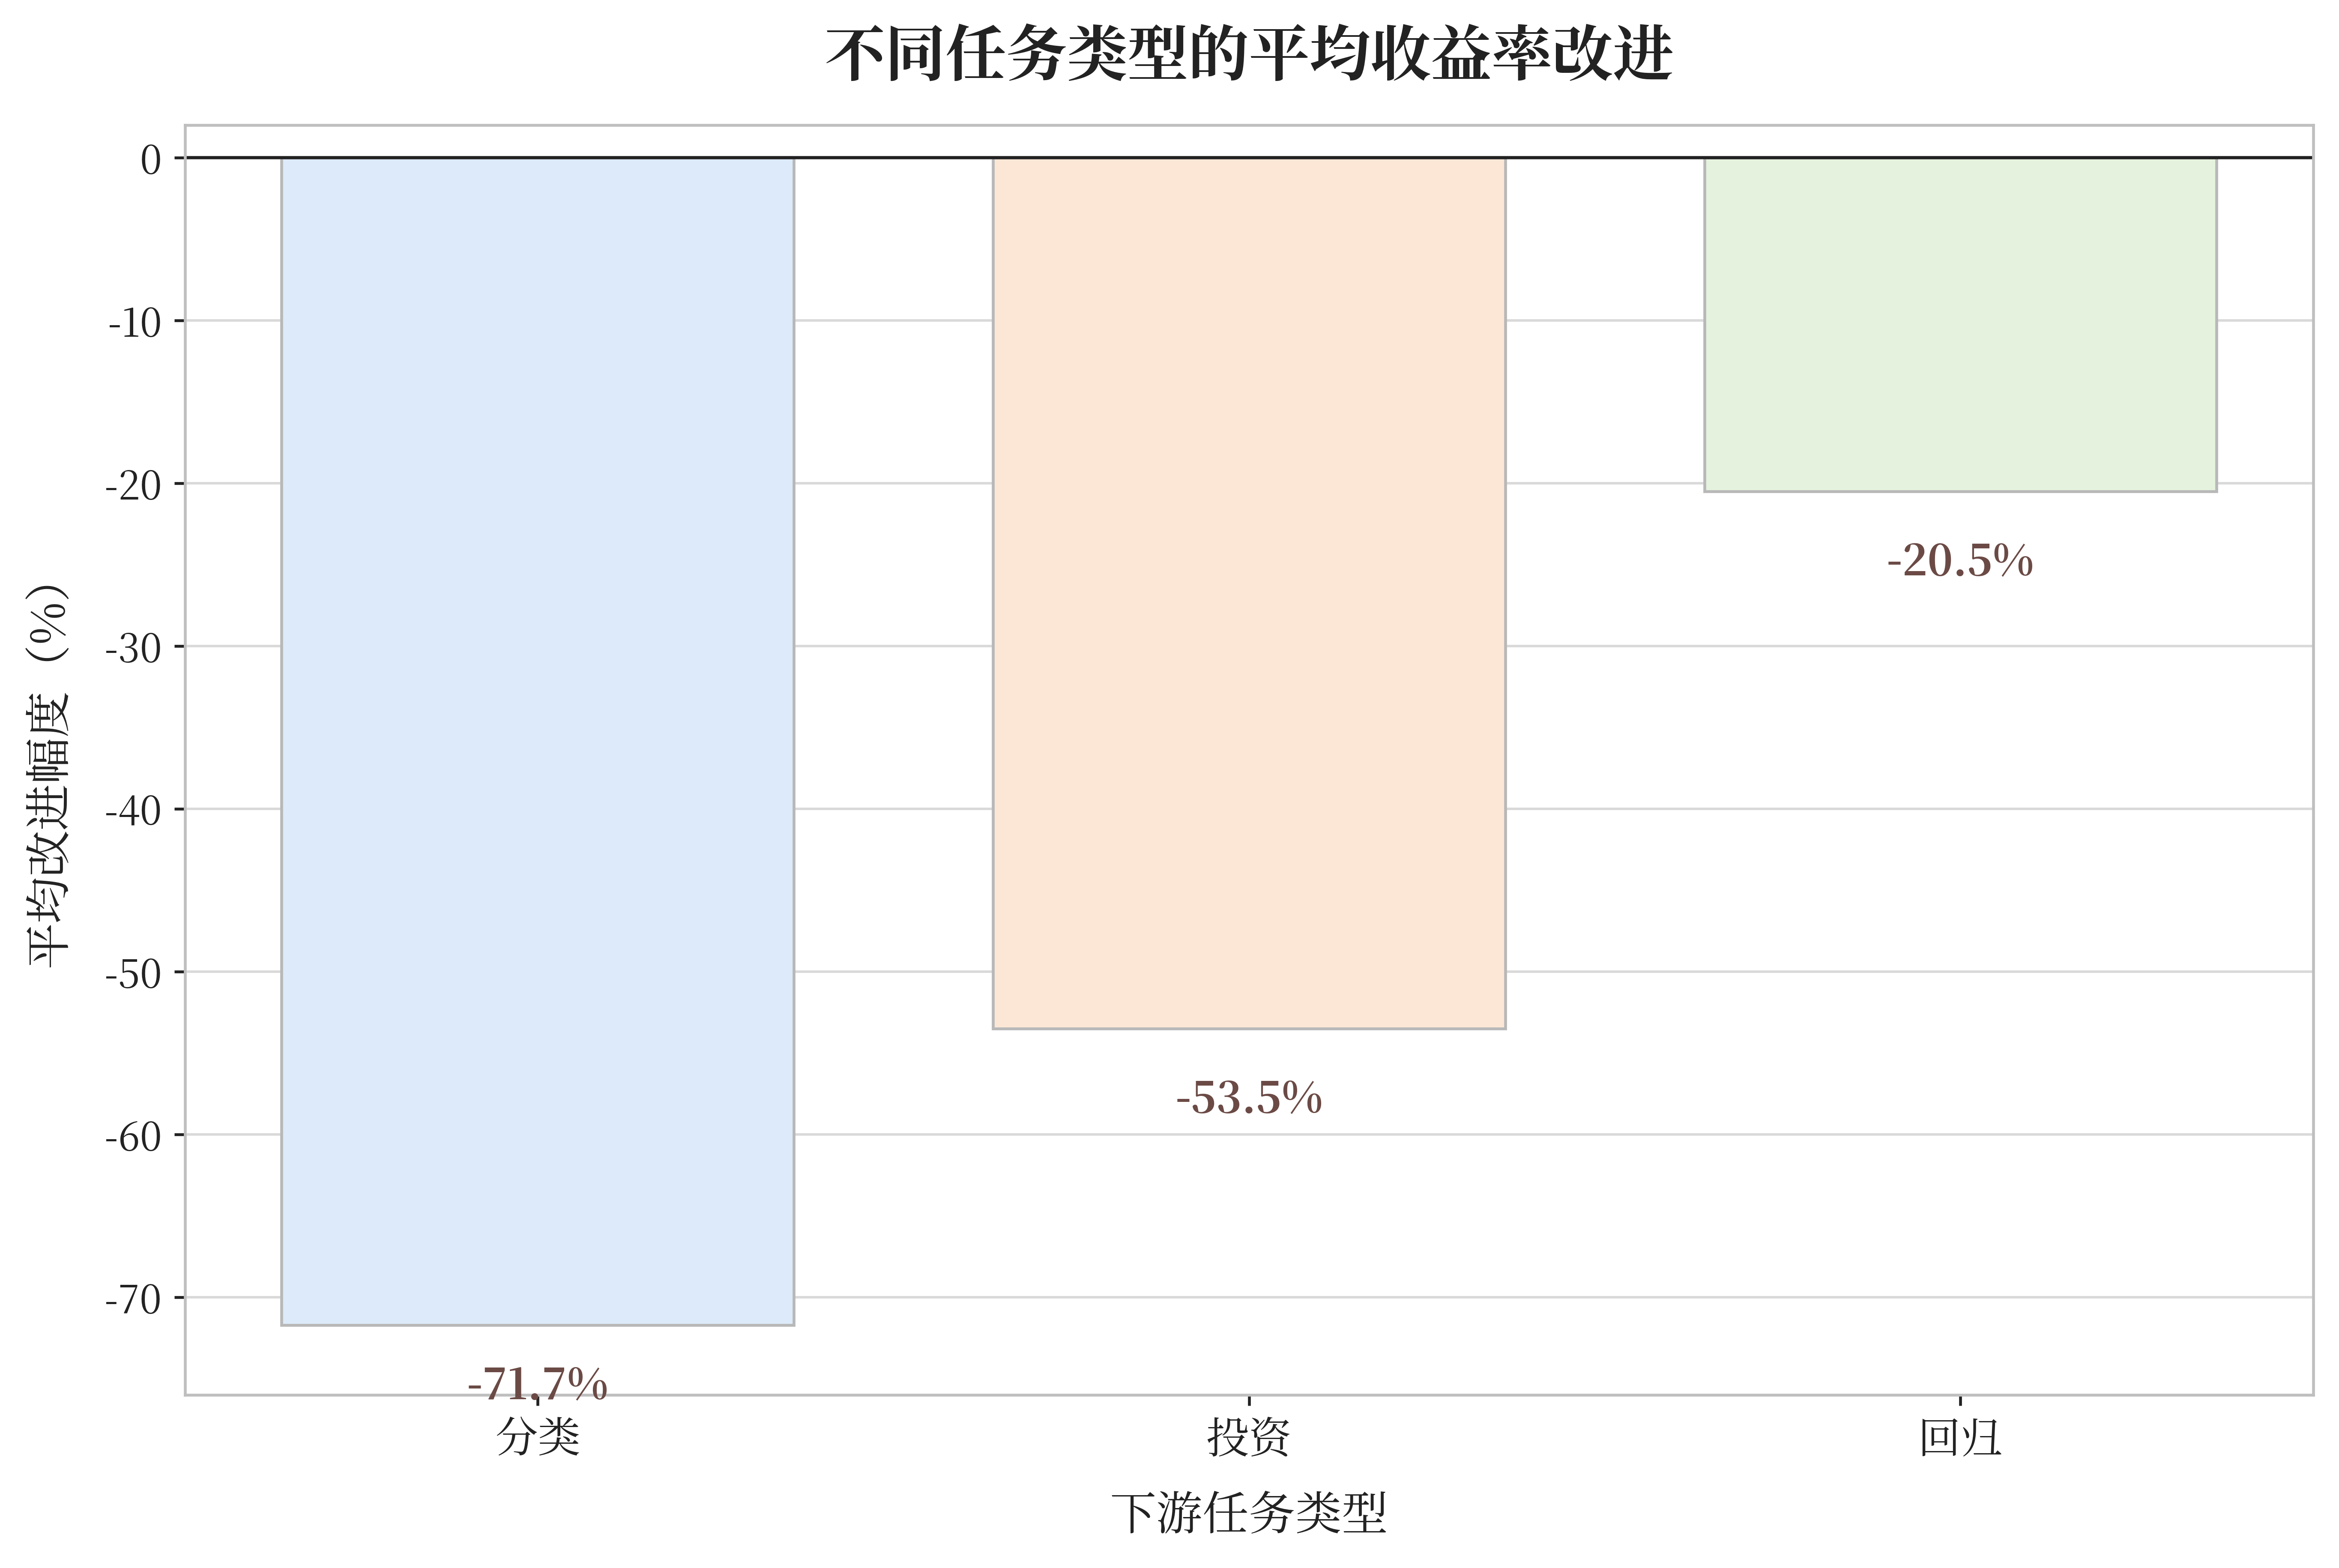
\includegraphics[width=0.8\textwidth]{figures/chap4/fig4_task_comparison_cn.png} 
    \caption{不同任务类型的平均收益改进幅度}
    \label{fig:highdimtaskcomp}
\end{figure}

三类任务中，回归任务的平均收益改进更为明显，棉花（+340\%）、动力煤（+195.51\%）、白糖（+36.40\%）均属增幅较大的案例。回归任务要求输出连续价格值，不同生成器在预测精度上的差异在连续空间中更容易被动态评估机制捕捉。动力煤是“亏损转盈利”的典型案例：基准模型回测亏损-16.23\%，赛马场竞争机制将其转为+15.50\%盈利。图\ref{fig:highdimcoalpredcom}先从价格预测层面对比两类模型的拟合效果，用于观察动态竞争是否改善了局部价格波动的跟踪能力。

% \begin{figure}[h!]
%     \centering 
%     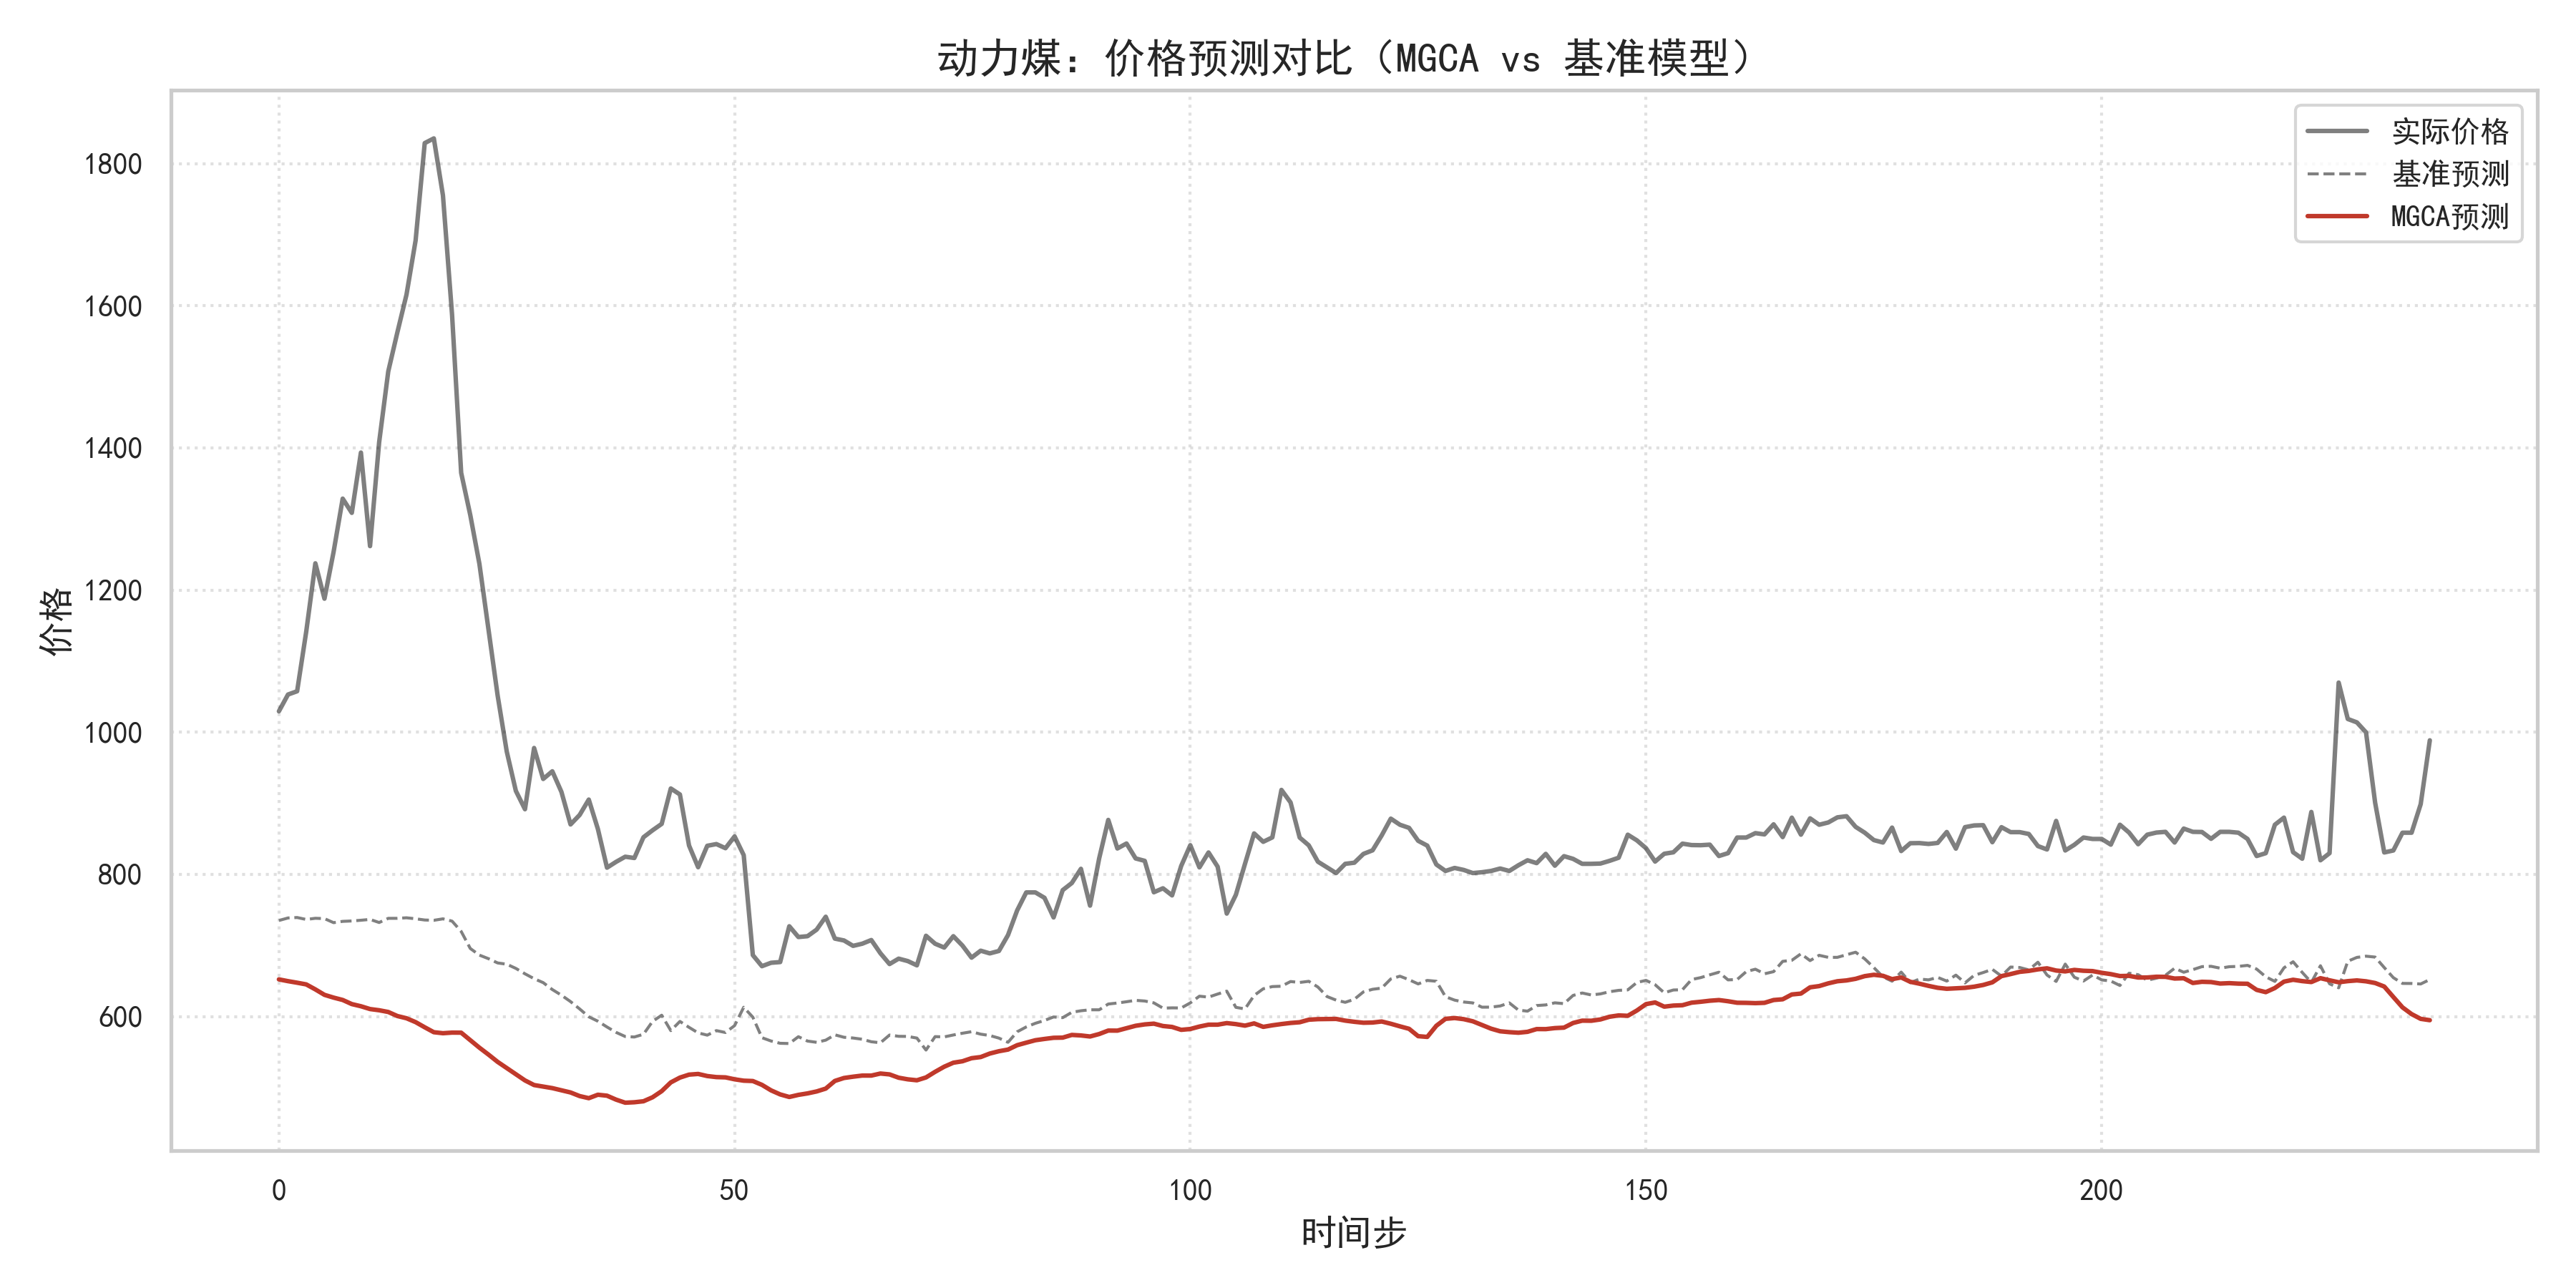
\includegraphics[width=0.8\textwidth]{figures/chap4/fig9_coal_pred_comparison_cn.png} 
%     \caption{动力煤价格逐日预测拟合对比}
%     \label{fig:highdimcoalpredcom}
% \end{figure}
\begin{figure}[!htbp]
    \centering 
    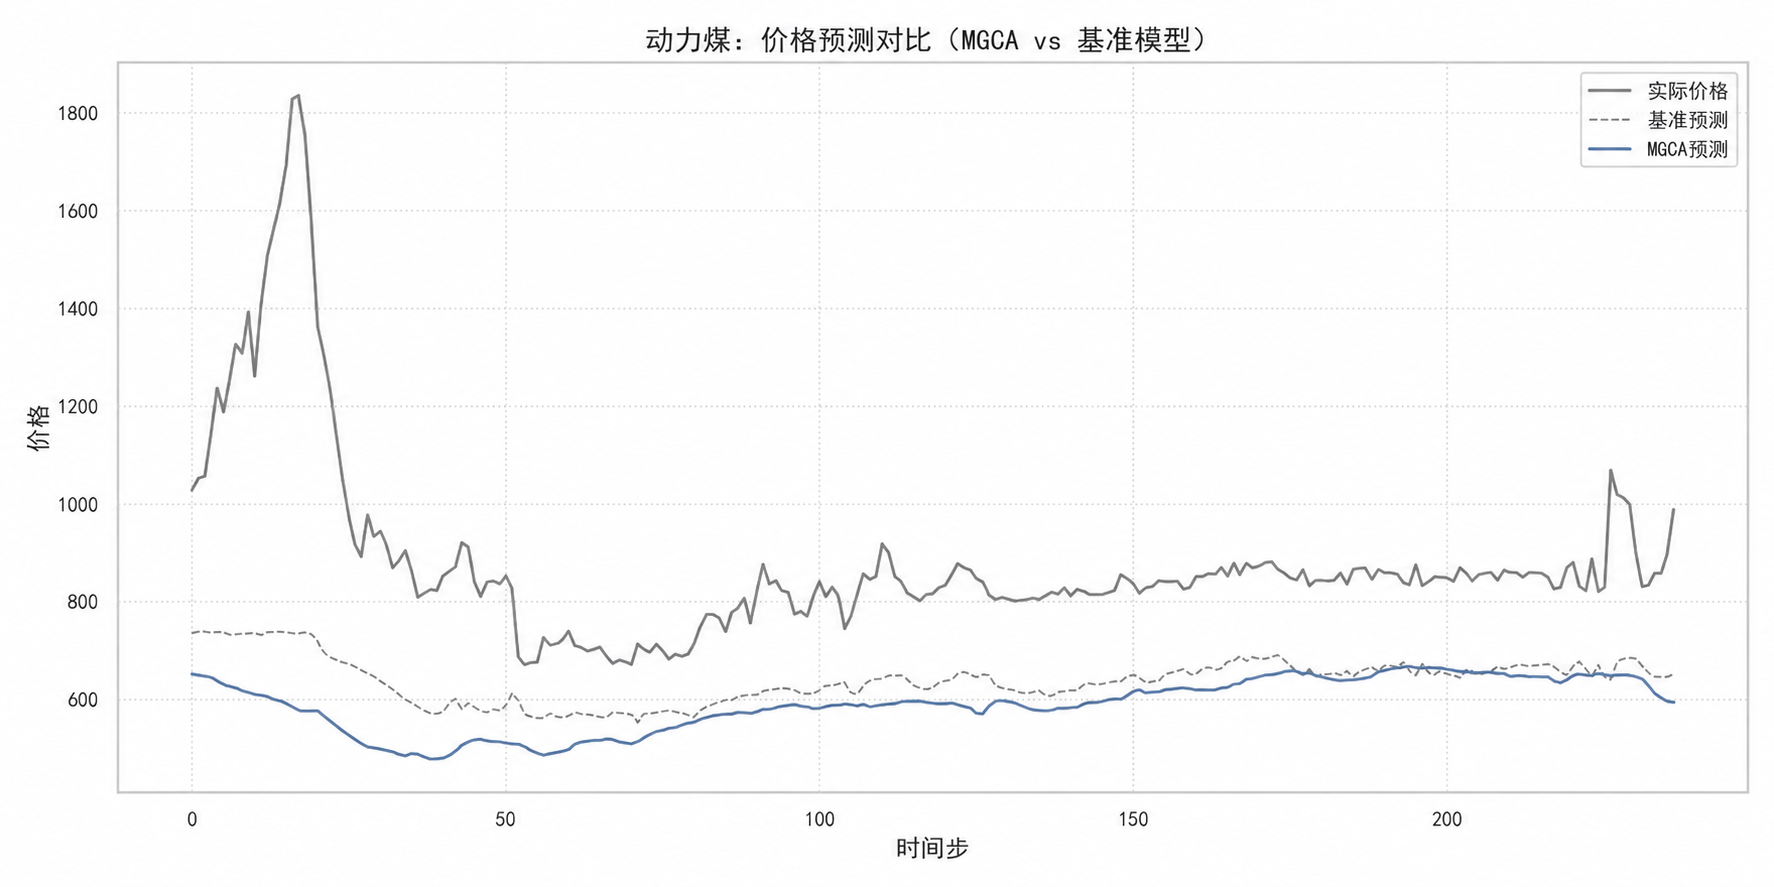
\includegraphics[width=0.8\textwidth]{figures/chap4/图3.8改.png} 
    \caption{动力煤价格逐日预测拟合对比}
    \label{fig:highdimcoalpredcom}
\end{figure}

若价格拟合改善能够转化为交易收益，则累计收益曲线应呈现更稳定的净值修复过程。图\ref{fig:highdimcoalequitycurve}进一步给出动力煤真实回测累计收益曲线，用于检验预测改善是否落实到回测收益层面。



% \begin{figure}[h!]
%     \centering 
%     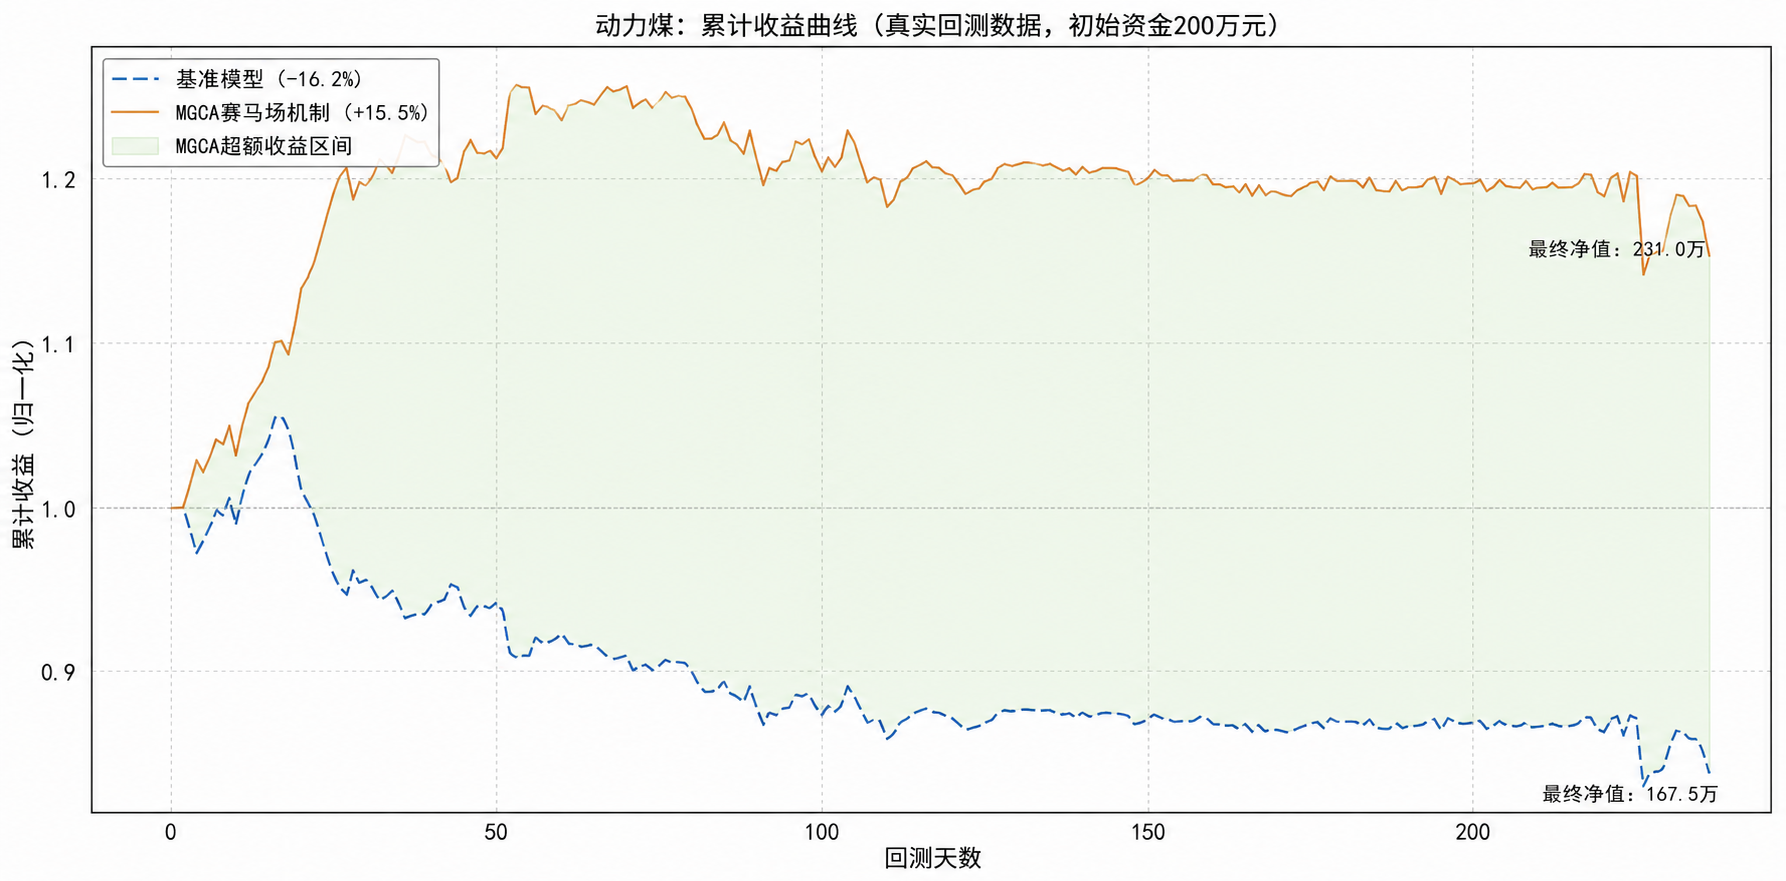
\includegraphics[width=0.8\textwidth]{figures/chap4/fig9_coal_equity_curve_cn.png} 
%     \caption{动力煤真实回测累计收益曲线（初始资金200万元）}
%     \label{fig:highdimcoalequitycurve}
% \end{figure}

\begin{figure}[!htbp]
    \centering 
    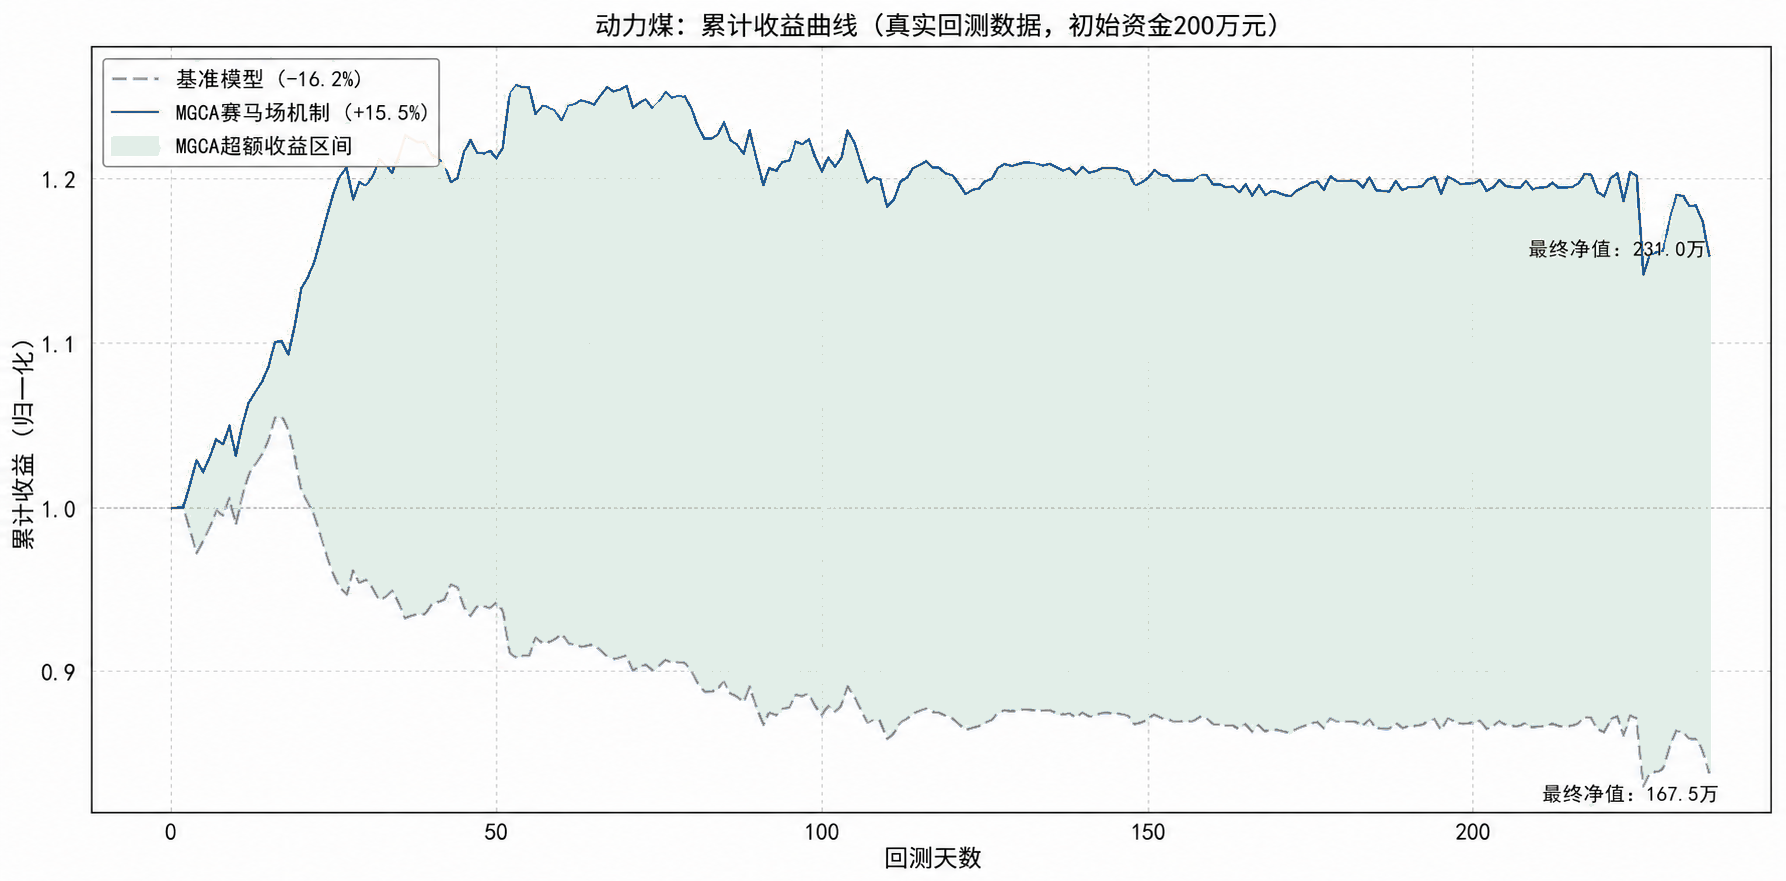
\includegraphics[width=0.8\textwidth]{figures/chap4/图3.9改.png} 
    \caption{动力煤真实回测累计收益曲线（初始资金200万元）}
    \label{fig:highdimcoalequitycurve}
\end{figure}

从动力煤案例看，赛马场竞争机制的作用不只是降低点预测误差，更重要的是在趋势变化阶段减少错误方向累积，使价格预测改善能够转化为收益曲线修复。
棉花（Cotton）是本章中改进幅度最大的单品案例。先从预测拟合层面看，图~\ref{fig:highdimcottonpredcomp}展示了棉花价格逐日预测拟合对比，赛马场竞争机制在价格急剧变化区间的预测误差低于基准模型。该图主要说明动态竞争机制能够在局部波动较强的区间中选择更适合当前状态的生成器输出。

% \begin{figure}[h!]
%     \centering 
%     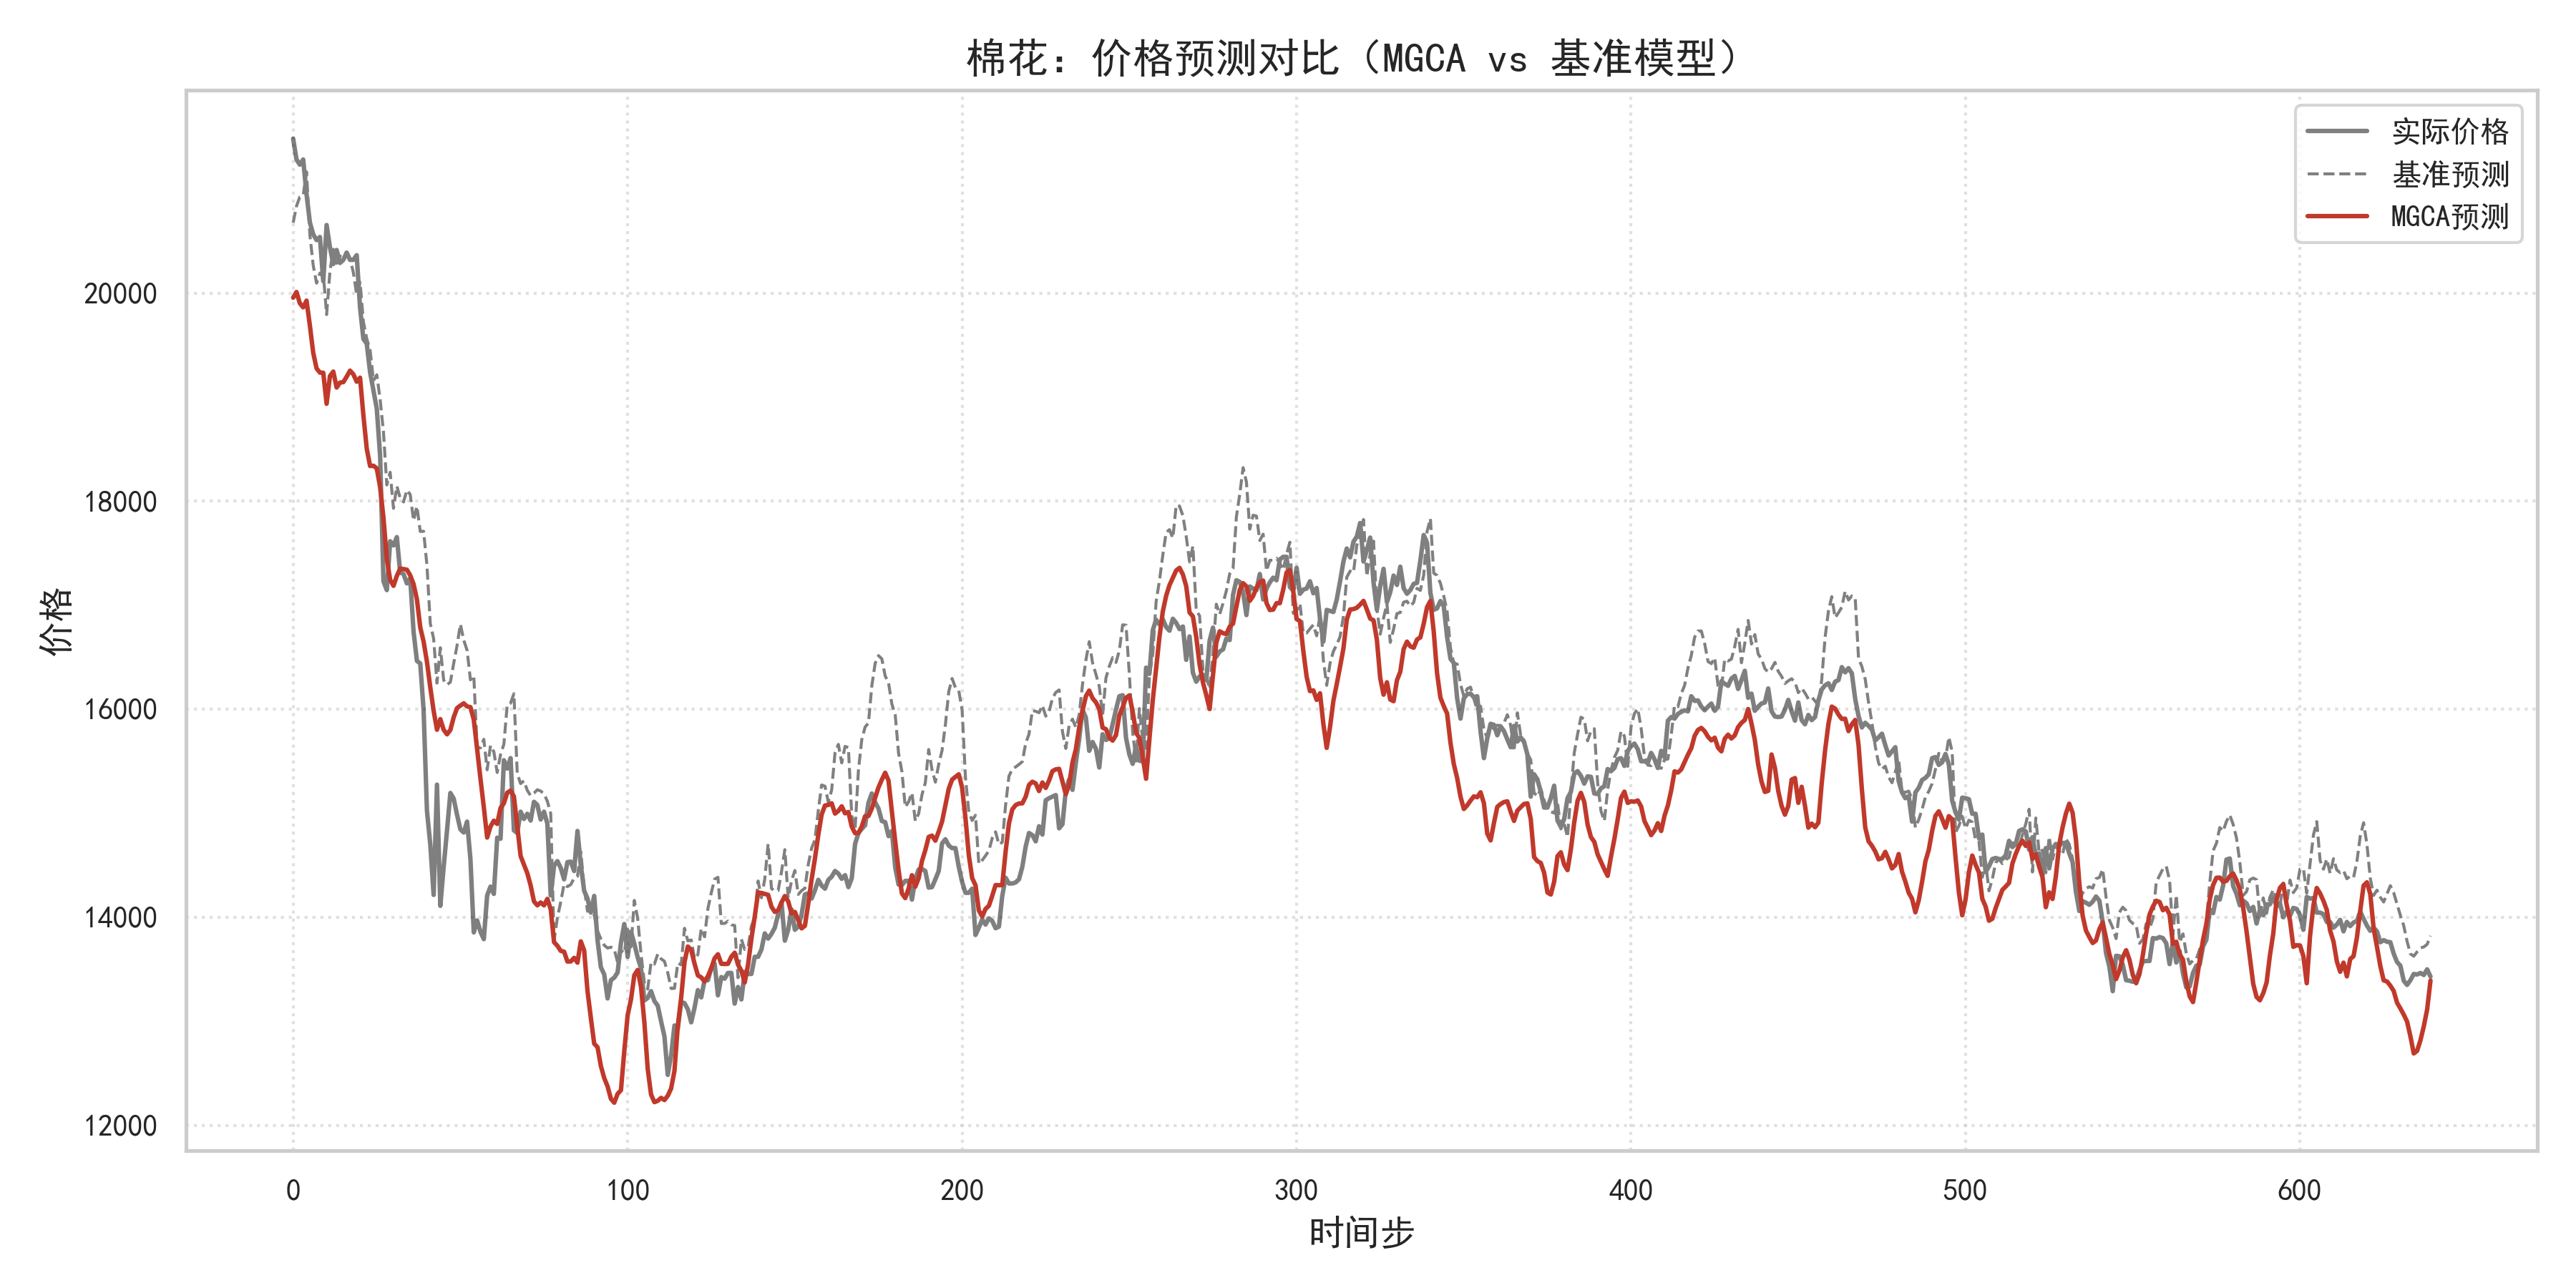
\includegraphics[width=0.8\textwidth]{figures/chap4/fig8_cotton_pred_comparison_cn.png} 
%     \caption{棉花价格逐日预测拟合对比}
%     \label{fig:highdimcottonpredcomp}
% \end{figure}

\begin{figure}[!htbp]
    \centering 
    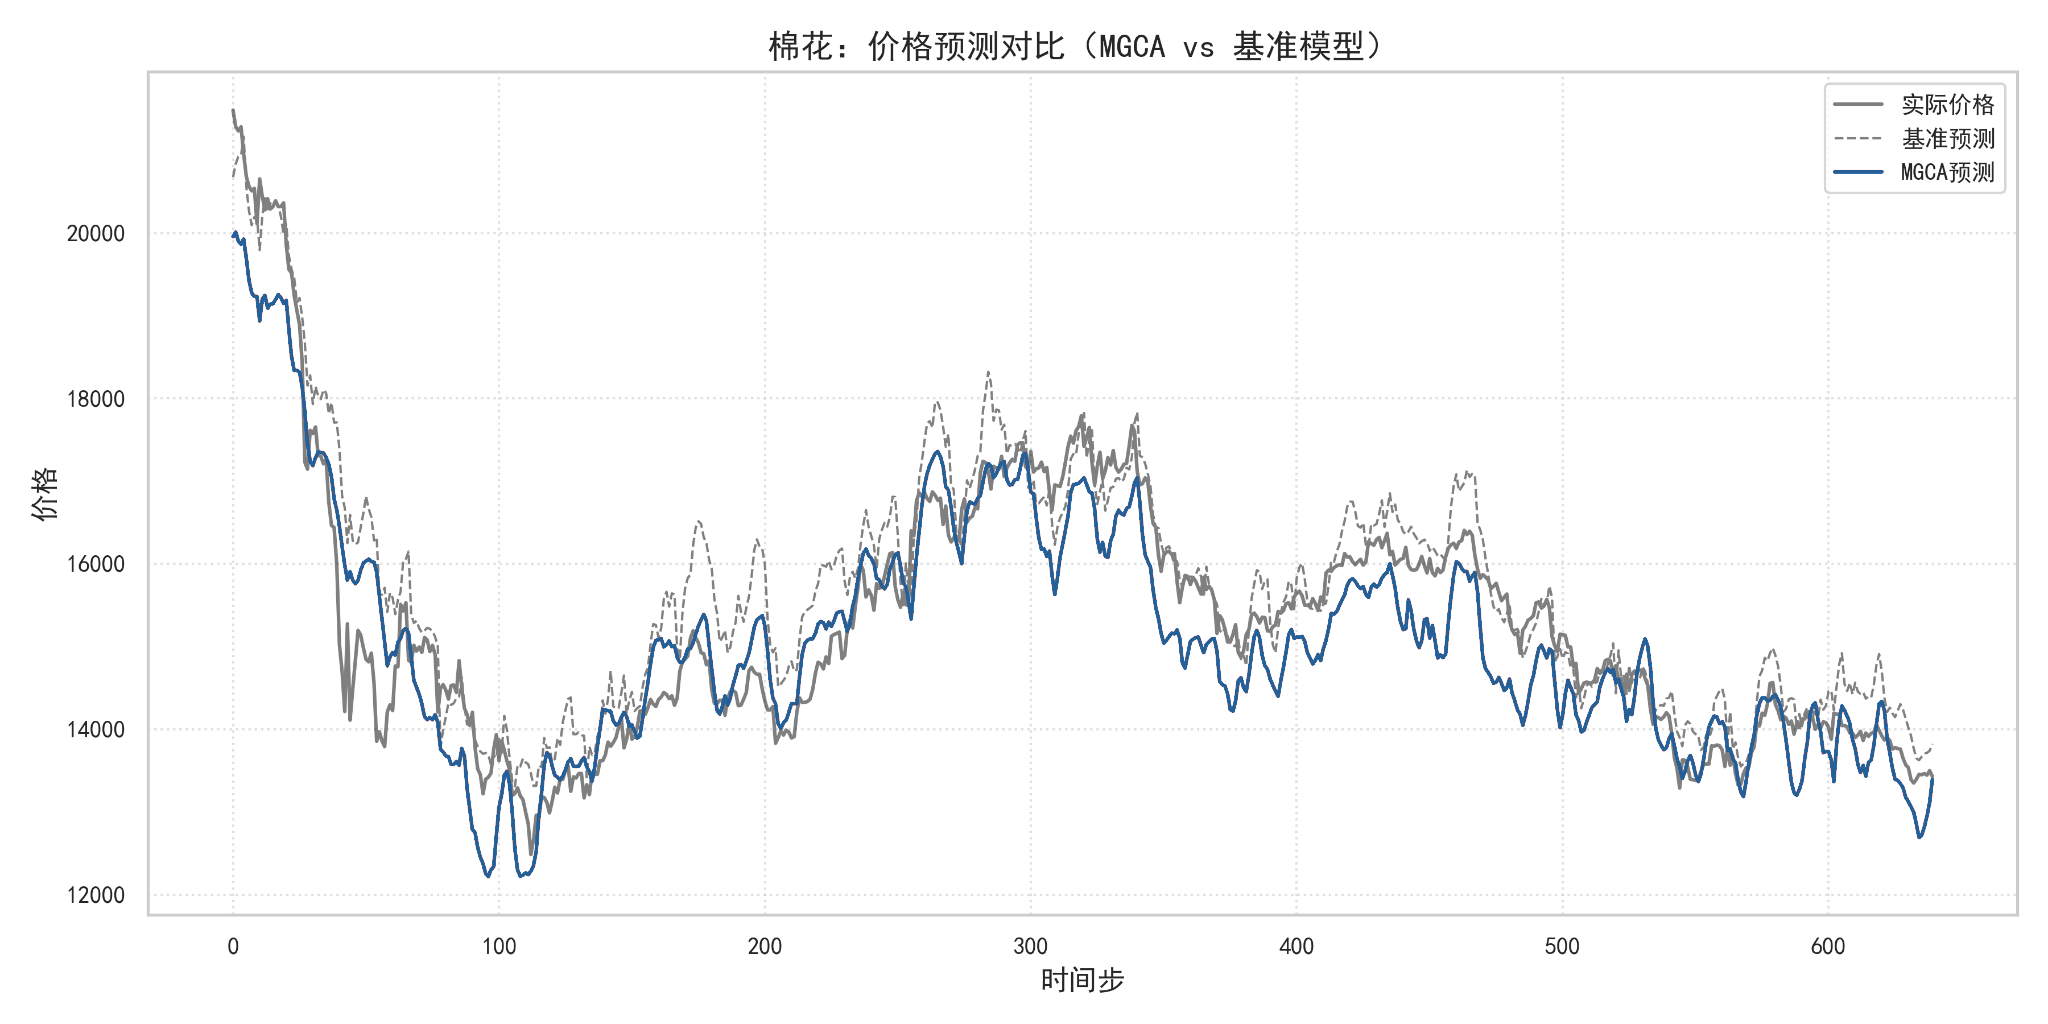
\includegraphics[width=0.8\textwidth]{figures/chap4/图3.10改.png} 
    \caption{棉花价格逐日预测拟合对比}
    \label{fig:highdimcottonpredcomp}
\end{figure}

进一步看，预测拟合优势是否具有交易意义，需要结合真实回测收益曲线进行判断。图~\ref{fig:highdimcottonequitycurve}呈现了棉花真实回测累计收益曲线，赛马场竞争机制最终收益+165.5\%（净值531万），高于基准模型的+37.6\%（净值275万）。


% \begin{figure}[h!]
%     \centering 
%     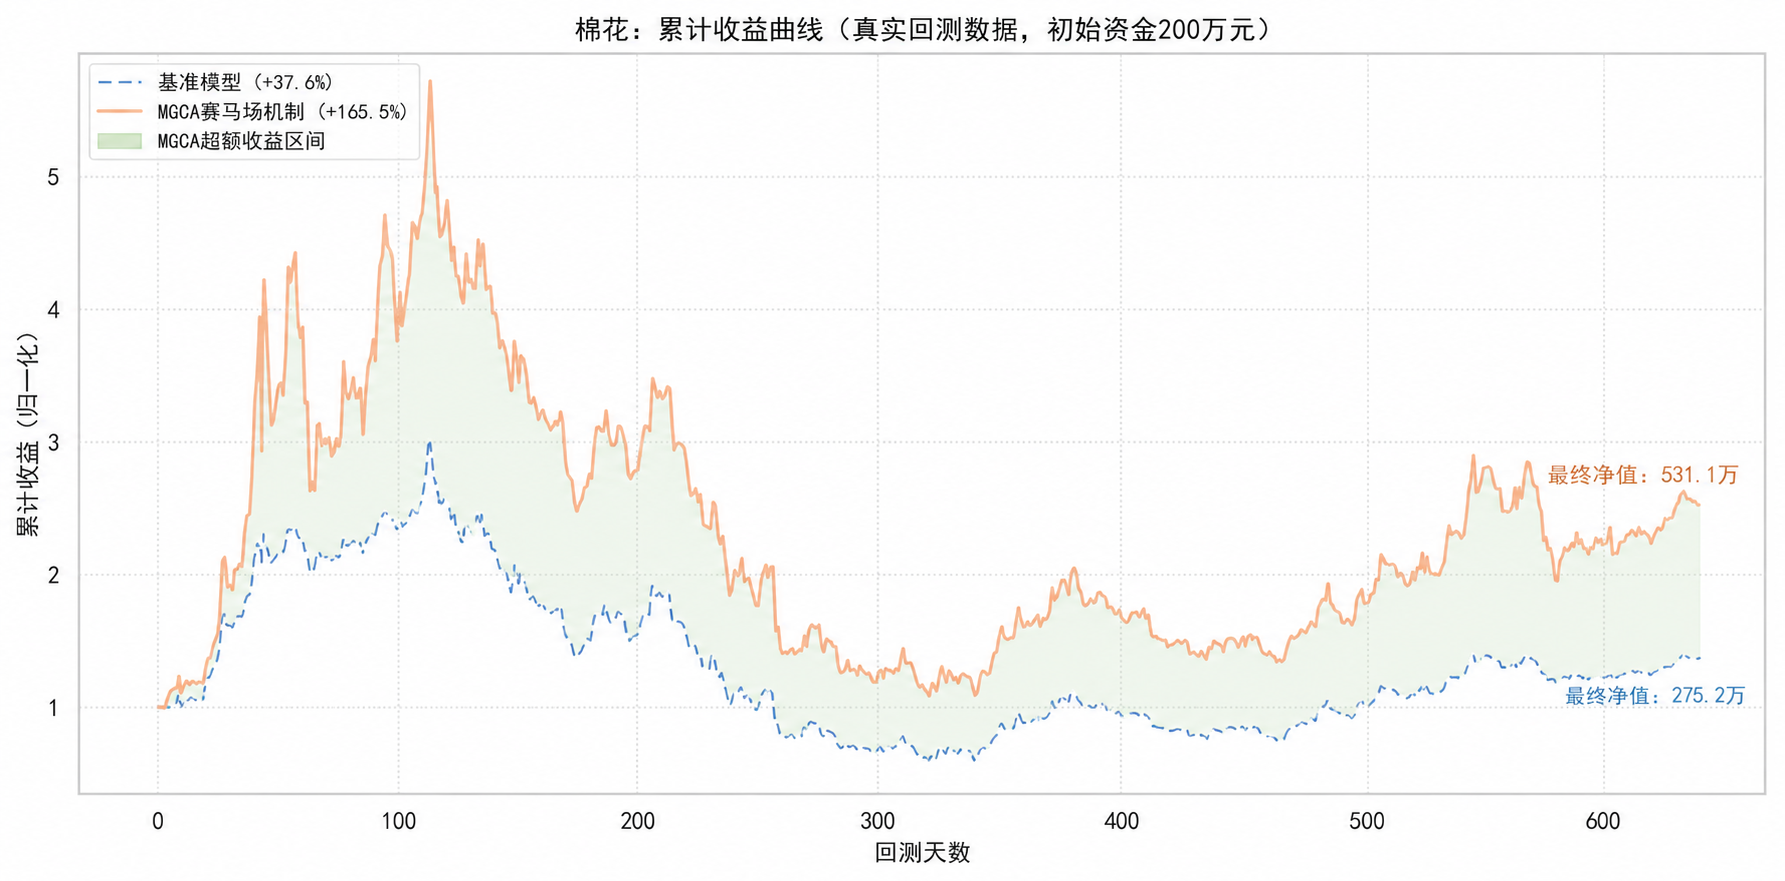
\includegraphics[width=0.8\textwidth]{figures/chap4/fig8_cotton_equity_curve_cn.png} 
%     \caption{棉花真实回测累计收益曲线}
%     \label{fig:highdimcottonequitycurve}
% \end{figure}
\begin{figure}[!htbp]
    \centering 
    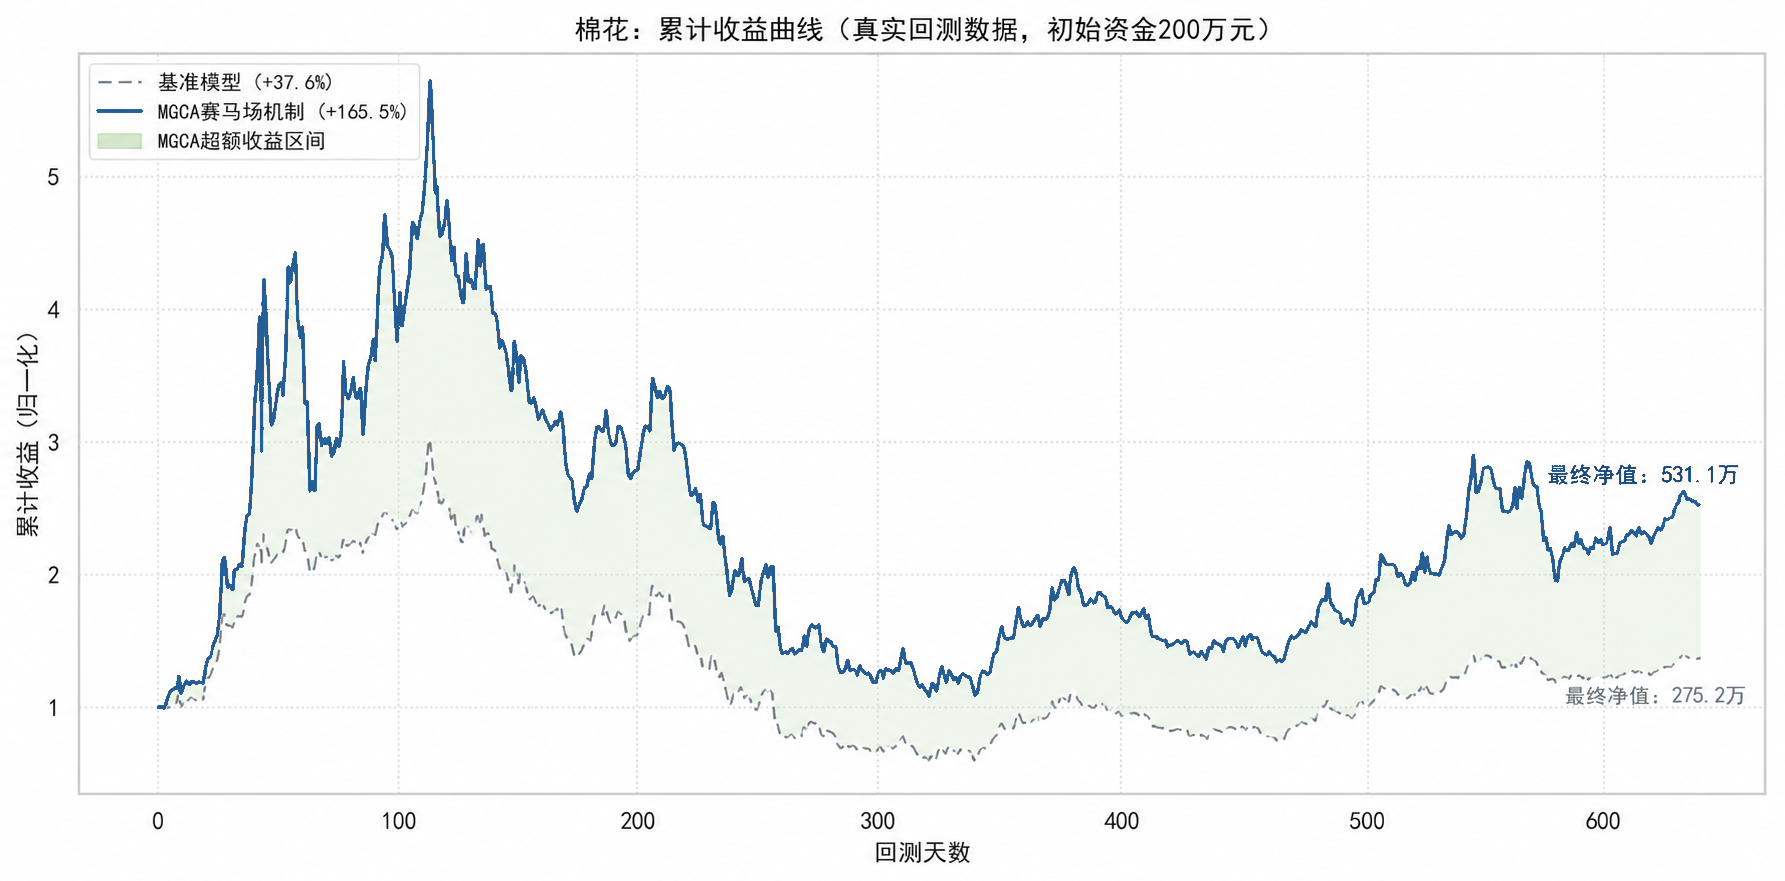
\includegraphics[width=0.8\textwidth]{figures/chap4/图3.11改.png} 
    \caption{棉花真实回测累计收益曲线}
    \label{fig:highdimcottonequitycurve}
\end{figure}

表~\ref{tab:cottoPerformance}进一步列出棉花回归任务的详细性能对比。该表用于补充说明收益提升并非只体现在曲线形态上，也反映在最终净值和收益率等量化指标中；同时，最大回撤略有增加，提示该案例的收益改善仍伴随一定风险代价。


\begin{table}[!htbp]
\centering
\caption{棉花（Cotton）回归任务详细性能对比}
\label{tab:cottoPerformance}
\small
\setlength{\tabcolsep}{4pt}
\renewcommand{\arraystretch}{1.15}
\begin{tabular}{>{\raggedright\arraybackslash}p{3.8cm} >{\centering\arraybackslash}p{2.6cm} >{\centering\arraybackslash}p{3.2cm} >{\centering\arraybackslash}p{2.2cm}}
\toprule
\textbf{指标} & \textbf{基准模型} & \textbf{赛马场竞争机制} & \textbf{变化} \\
\midrule
策略收益率 (Return \%) & 37.58\% & \textbf{165.33\%} & \textbf{+340.00\%} \\
最终净值 (Final Value) & ¥2,751,503 & \textbf{¥5,306,581} & \textbf{+92.86\%} \\
最大回撤 (Max Drawdown) & 80.34\% & 81.02\% & +0.85\% \\
初始资本 (Initial Capital) & ¥2,000,000 & ¥2,000,000 & -- \\
回测交易日 (Trading Days) & 639 & 639 & -- \\
\bottomrule
\end{tabular}
\end{table}

为解释棉花案例中的收益改善来源，后续图表进一步观察模型群体内部的动态选择过程。图~\ref{fig:highdimcottonradar}从多生成器排名热力图角度展示不同生成器在训练与评估过程中的相对位置变化。


% \begin{figure}[h!]
%     \centering 
%     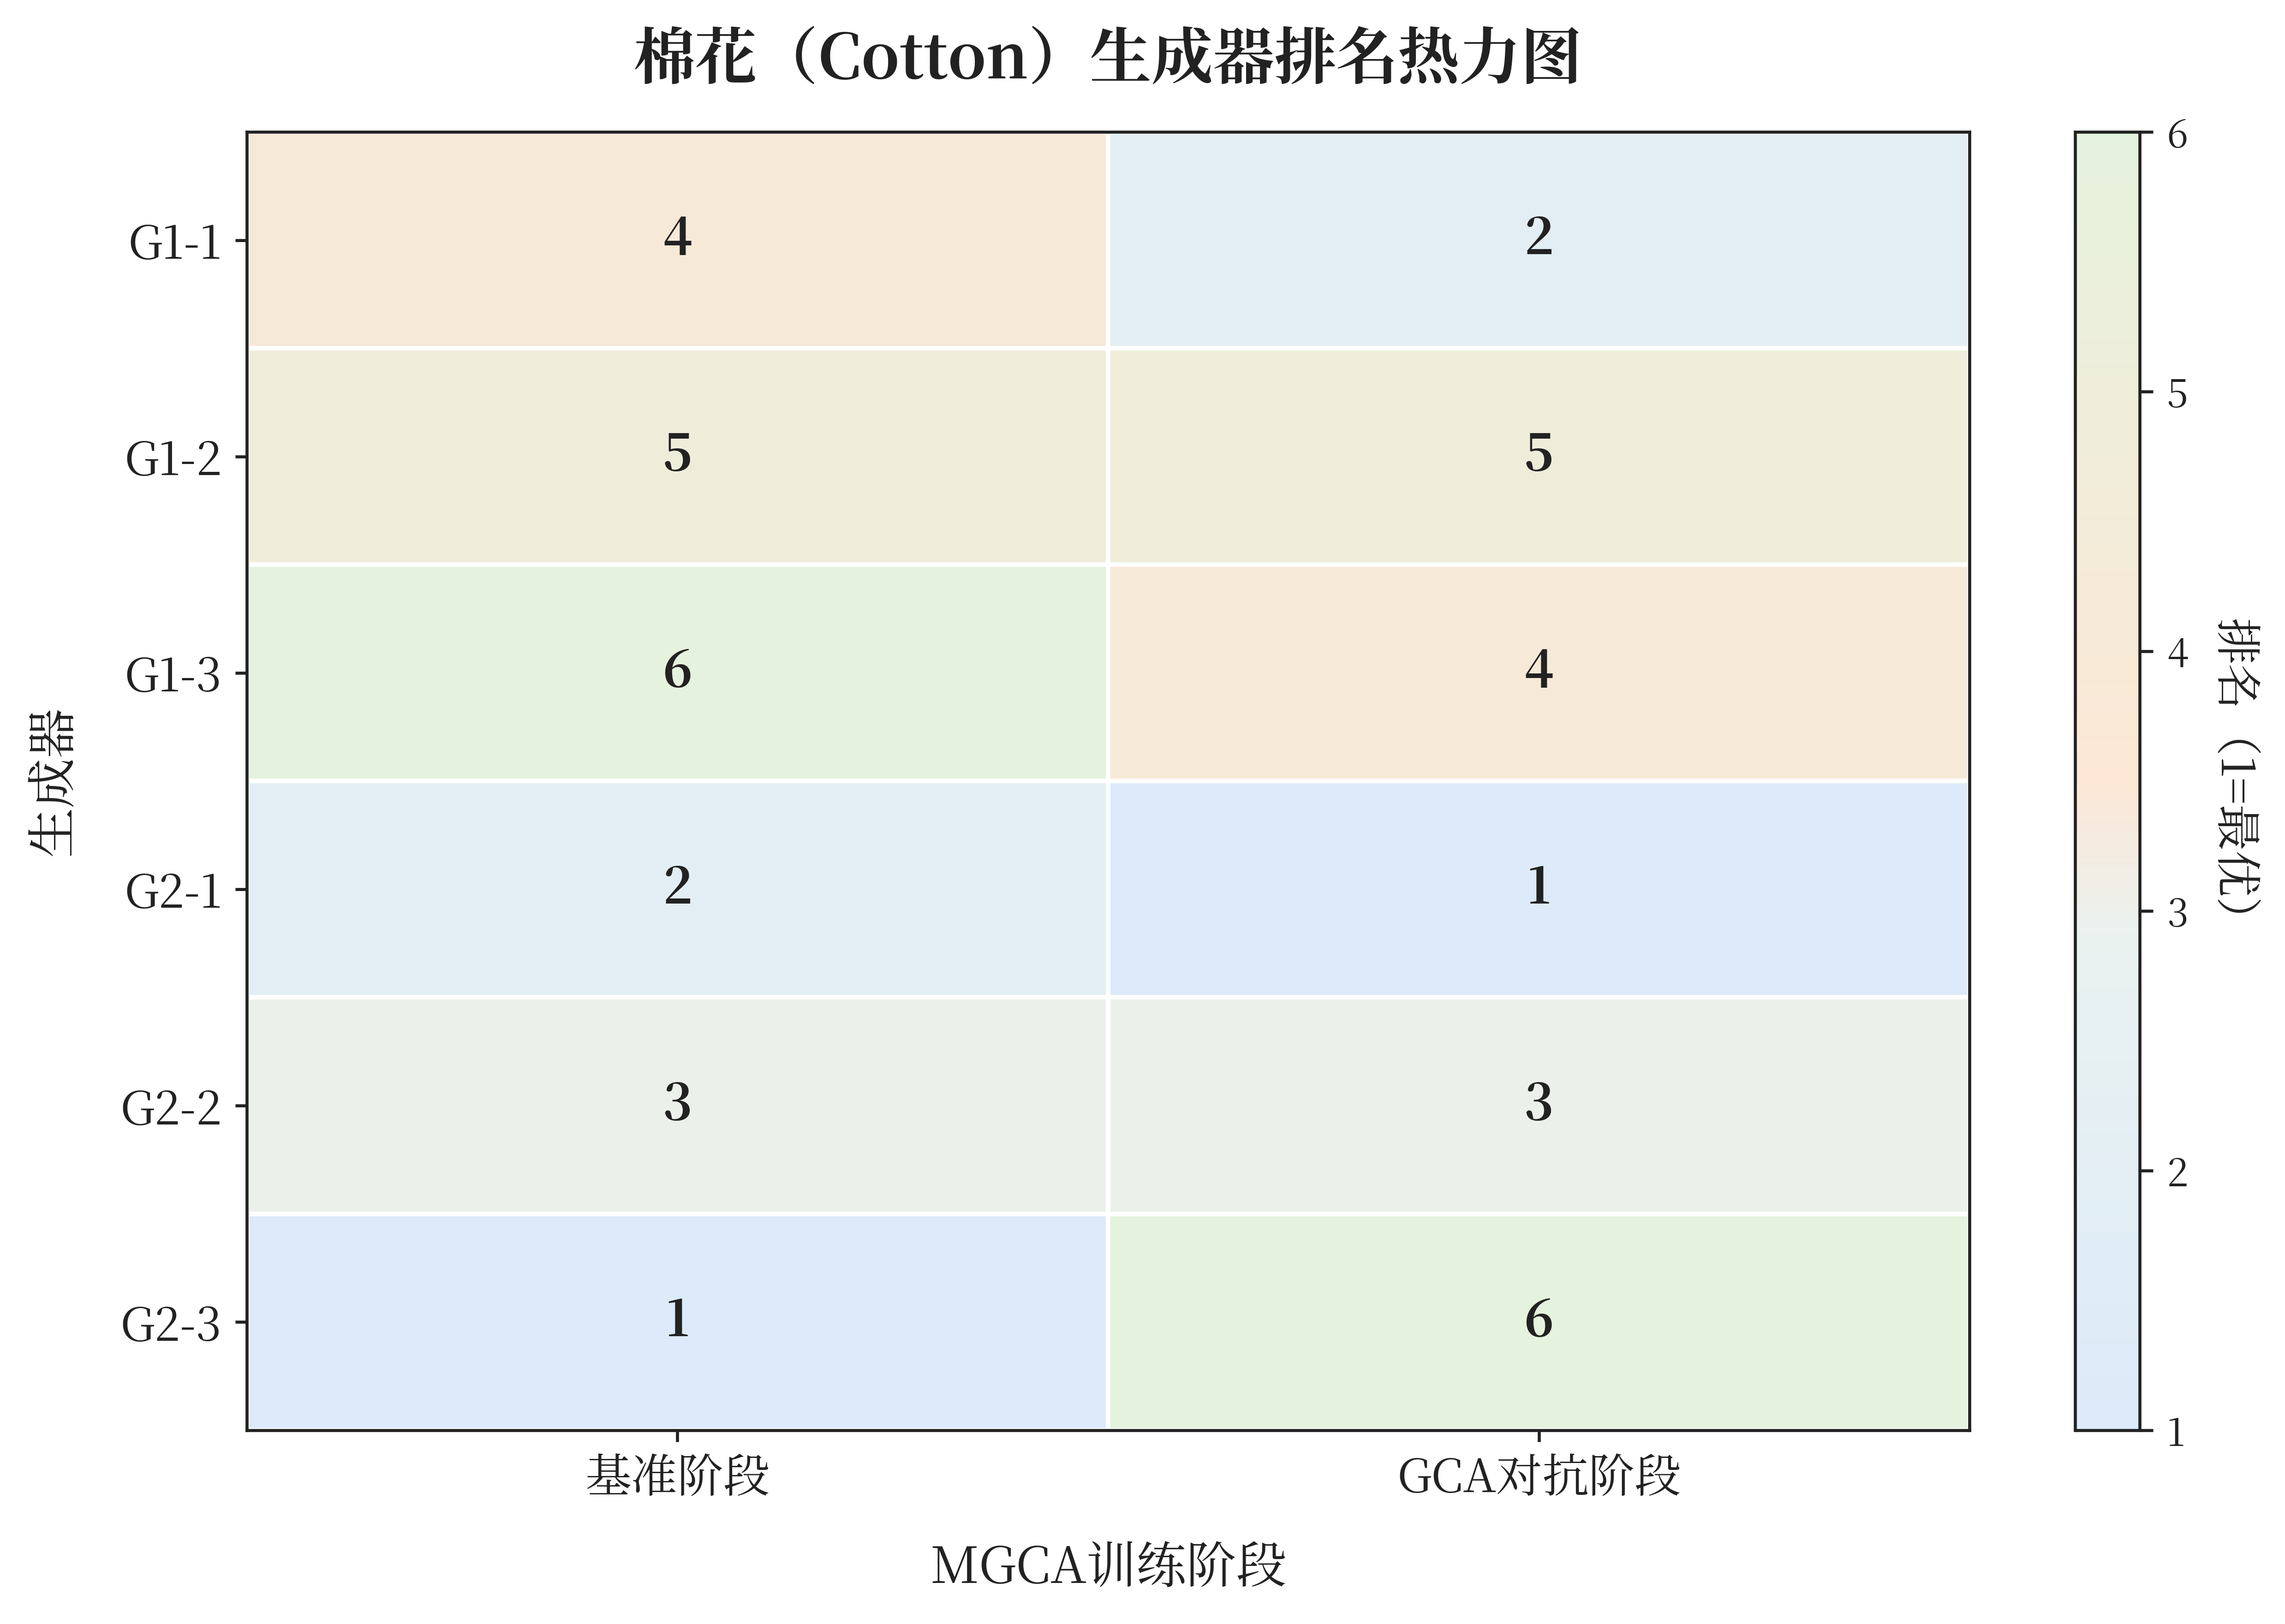
\includegraphics[width=0.8\textwidth]{figures/chap4/fig_cotton_ranking_heatmap_cn.png} 
%     \caption{棉花回归任务多生成器排名热力图}
%     \label{fig:highdimcottonradar}
% \end{figure}

\begin{figure}[!htbp]
    \centering 
    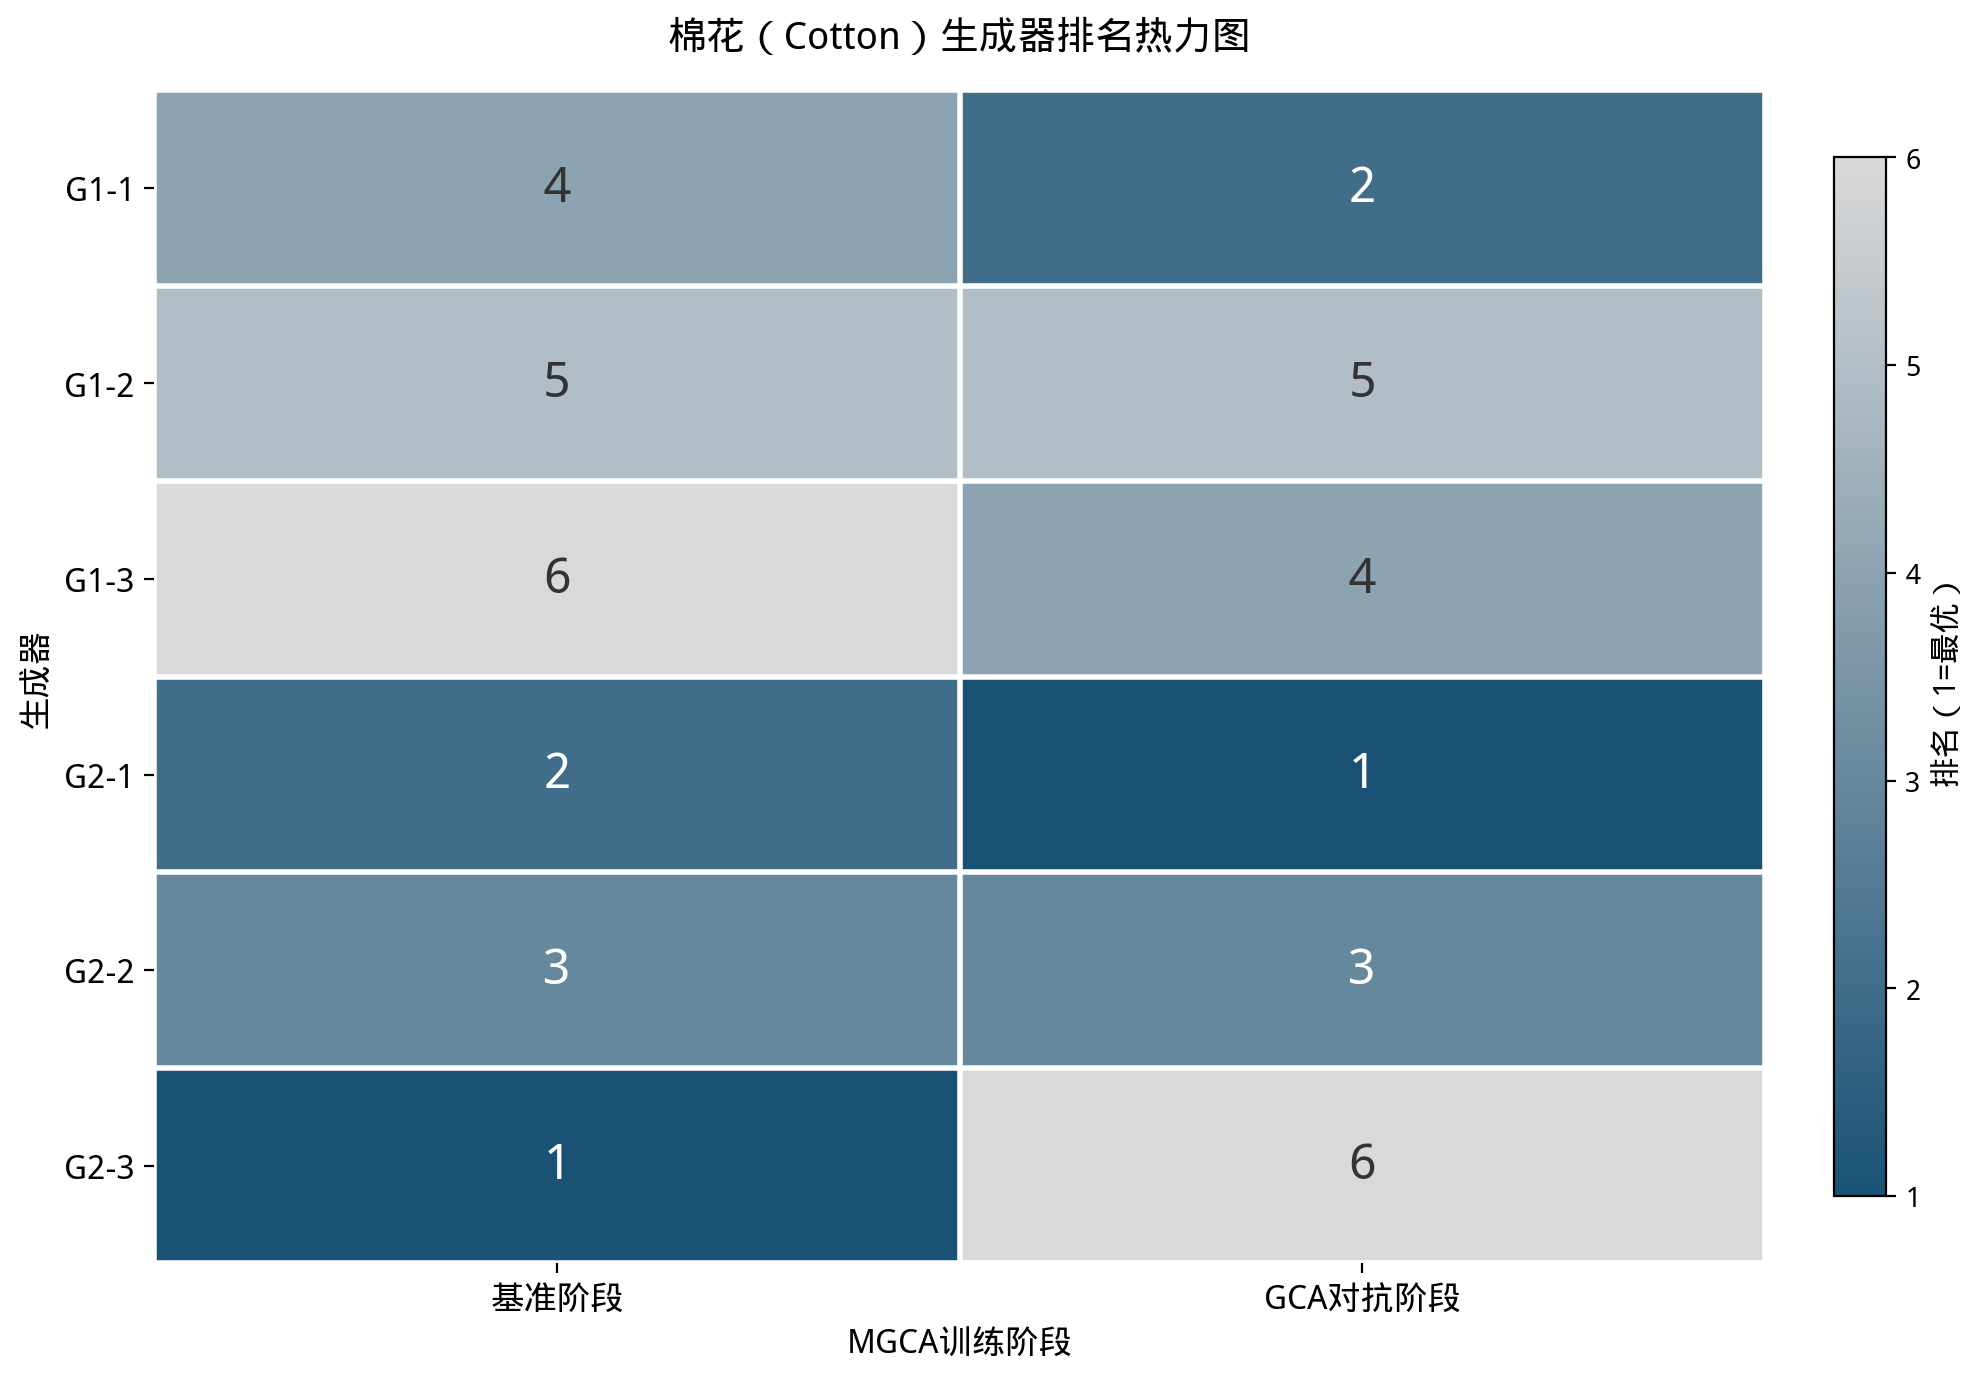
\includegraphics[width=0.8\textwidth]{figures/chap4/图3.12改.png} 
    \caption{棉花回归任务多生成器排名热力图}
    \label{fig:highdimcottonradar}
\end{figure}

图~\ref{fig:highdimcottonhm}则从多维性能雷达图角度补充观察棉花案例中的收益、回撤和风险调整表现。两张图共同说明，棉花案例的改进不是单一模型偶然胜出，而是动态选择机制在不同生成器之间持续比较后的结果。


\begin{figure}[!htbp]
    \centering 
    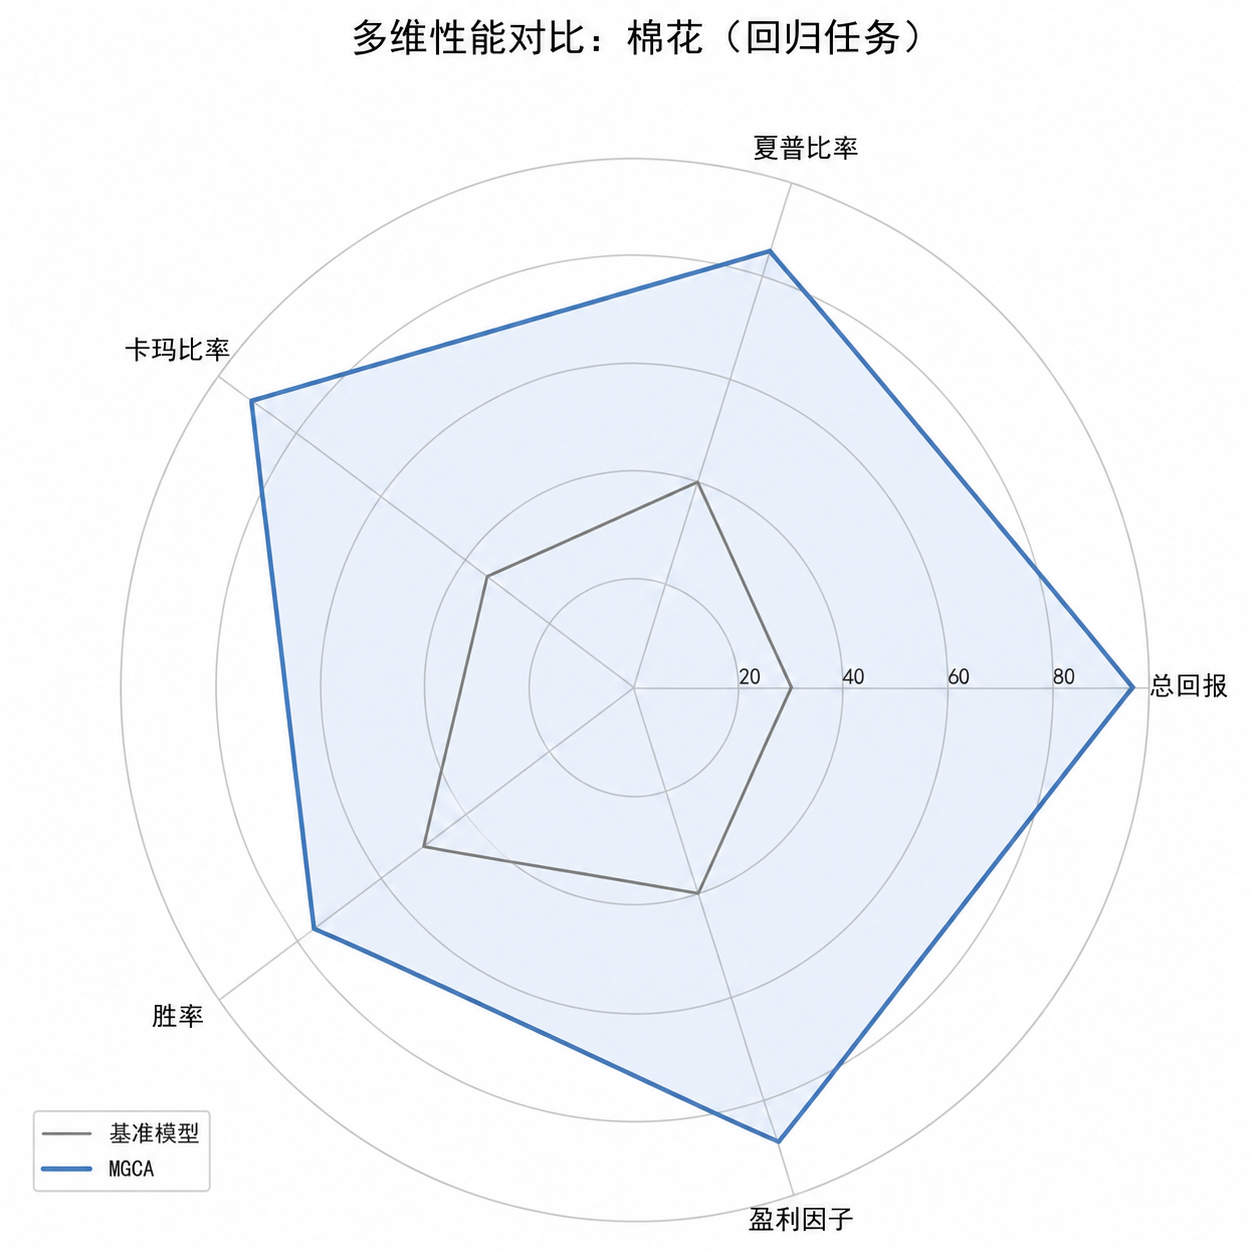
\includegraphics[width=0.8\textwidth]{figures/chap4/fig6_radar_cotton_cn.png}
    \caption{棉花回归任务多维性能雷达图}
    \label{fig:highdimcottonhm}
\end{figure}

在典型案例分析之后，进一步需要考察赛马场竞争机制是否改变了模型学习过程本身。图\ref{fig:highdimtrainingmsecomp}展示了All-Assets组中16种资产在回归任务下赛马场竞争机制与基准模型的训练均方误差对比，以均方误差比率（赛马场竞争机制/基准模型）的形式呈现，小于1.0表示赛马场竞争机制的训练误差更低。该图的目的不是证明所有资产的训练误差都降低，而是观察动态竞争机制是否在不同品种上形成差异化学习效果。

% \begin{figure}[htbp]
%     \centering 
%     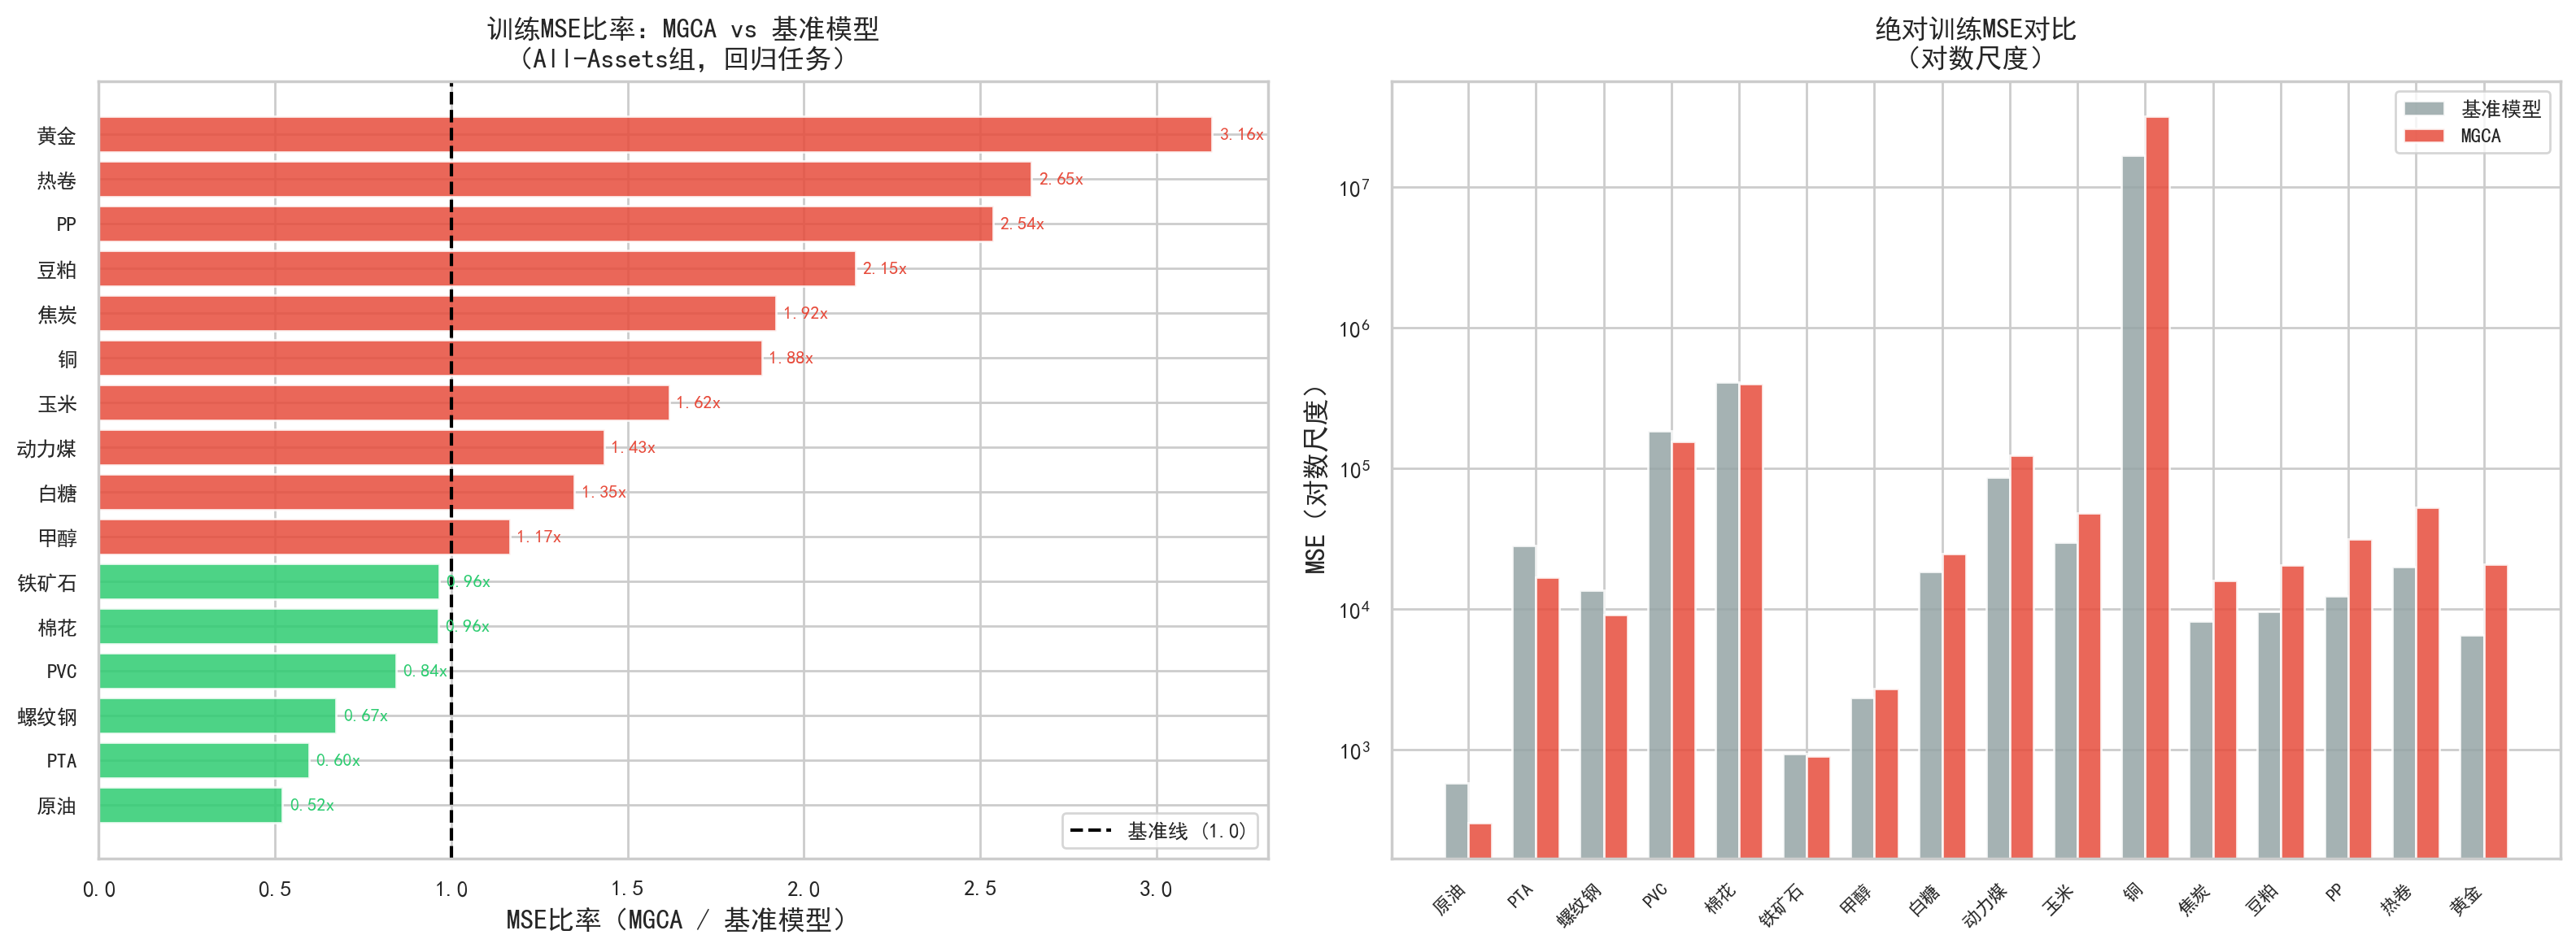
\includegraphics[width=0.8\textwidth]{figures/chap4/fig15_training_mse_comparison_cn.png} 
%     \caption{训练均方误差对比（All-Assets组，回归任务）}
%     \label{fig:highdimtrainingmsecomp}
% \end{figure}

\begin{figure}[!htbp]
    \centering 
    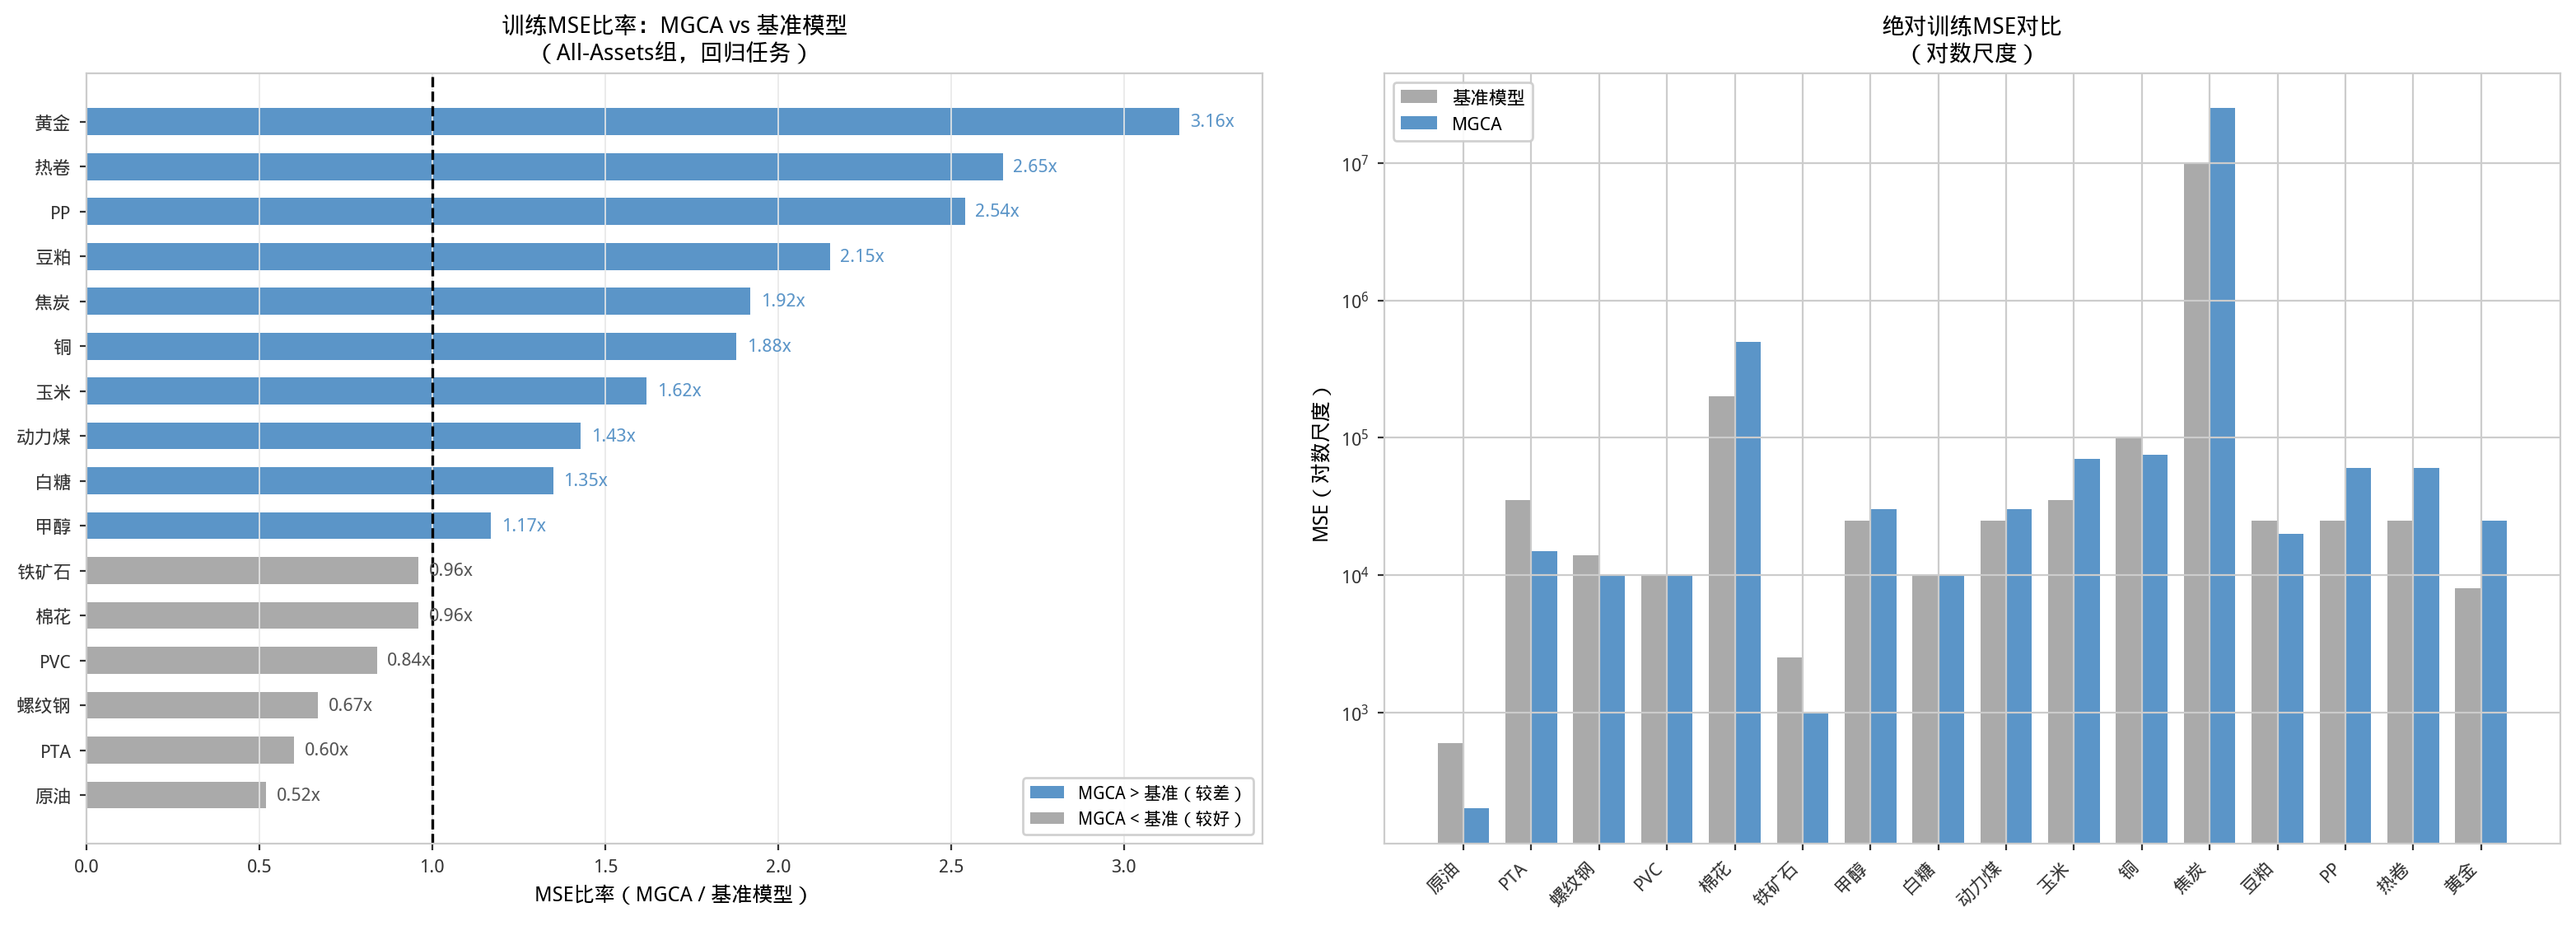
\includegraphics[width=0.8\textwidth]{figures/chap4/图3.14改.png} 
    \caption{训练均方误差对比（All-Assets组，回归任务）}
    \label{fig:highdimtrainingmsecomp}
\end{figure}

赛马场竞争机制在训练均方误差上的表现并不均匀。Crude Oil（0.52x）、PTA（0.60x）、Rebar（0.67x）等资产上训练误差低于基准模型；而Gold（3.16x）、Hot Rolled Coil（2.65x）等资产上训练均方误差反而更高。这一差异表明，赛马场竞争机制并非单纯以最小化训练误差为目标，而是在多个生成器之间保持“探索-利用”的平衡。训练均方误差的增加，可能是保持生成器多样性的代价之一。

分类任务直接衡量模型预测价格涨跌方向的能力。图\ref{fig:highdimtrainingACCcomp}展示了赛马场竞争机制与基准模型在所有资产组和品种上的分类准确率差异。

% \begin{figure}[htbp]
%     \centering 
%     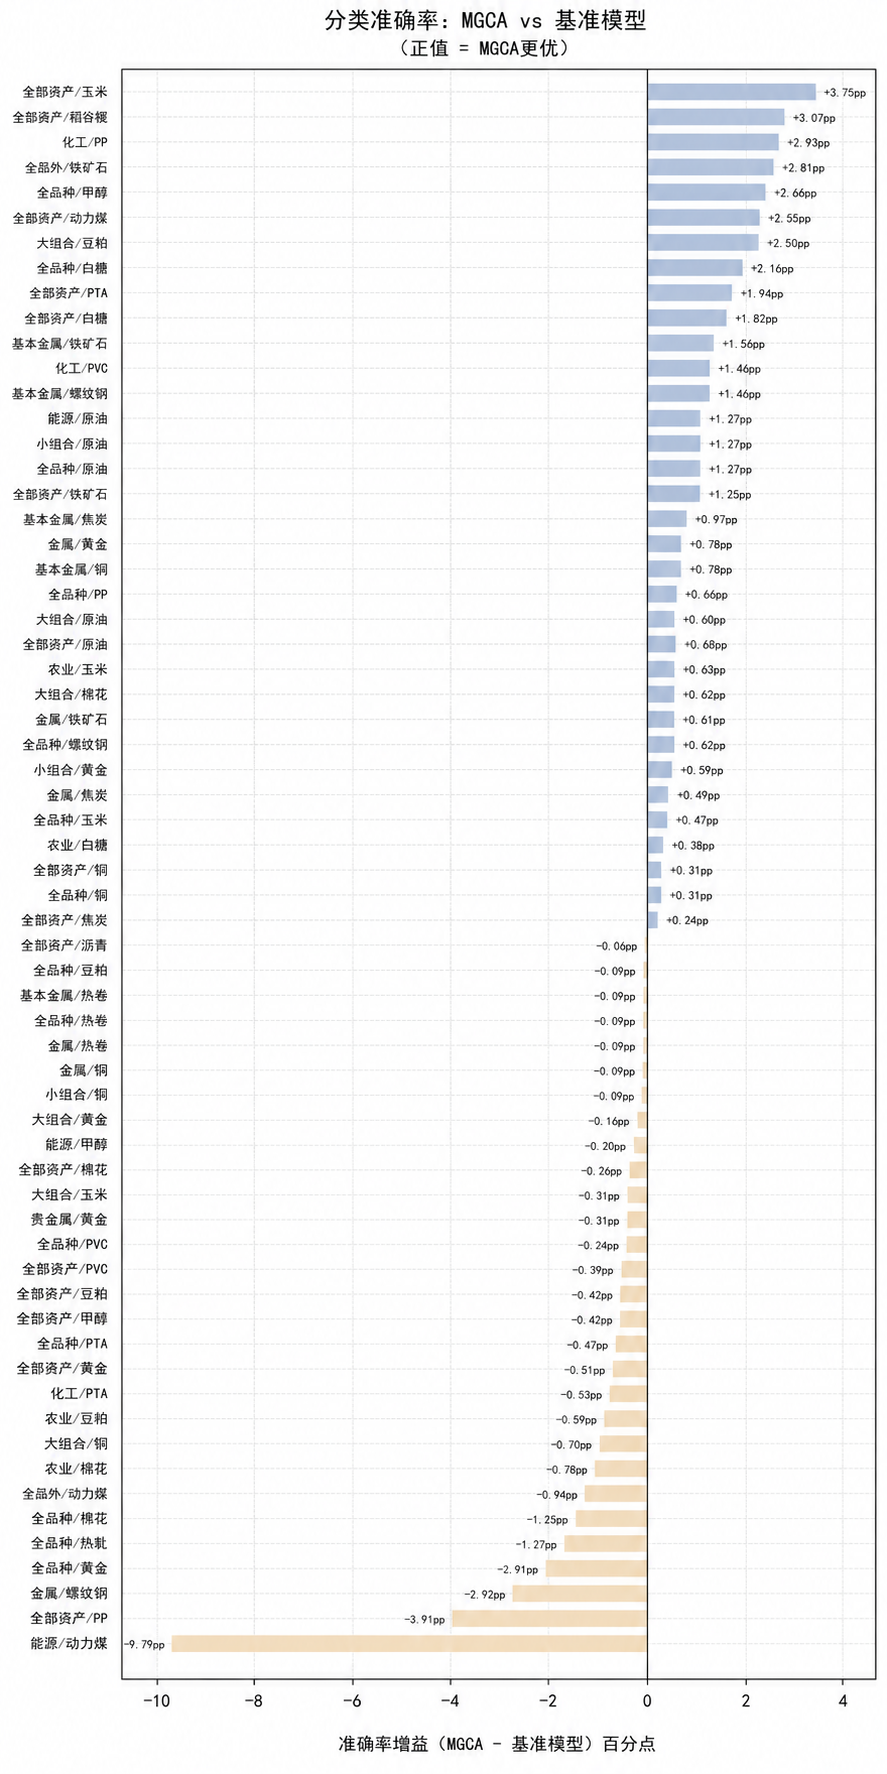
\includegraphics[width=0.8\textwidth,max height=0.75\textheight,keepaspectratio]{figures/chap4/fig16_classification_accuracy_cn.png} 
%     \caption{分类准确率差异（赛马场竞争机制 vs. 基准模型）}
%     \label{fig:highdimtrainingACCcomp}
% \end{figure}

\begin{figure}[!htbp]
    \centering 
    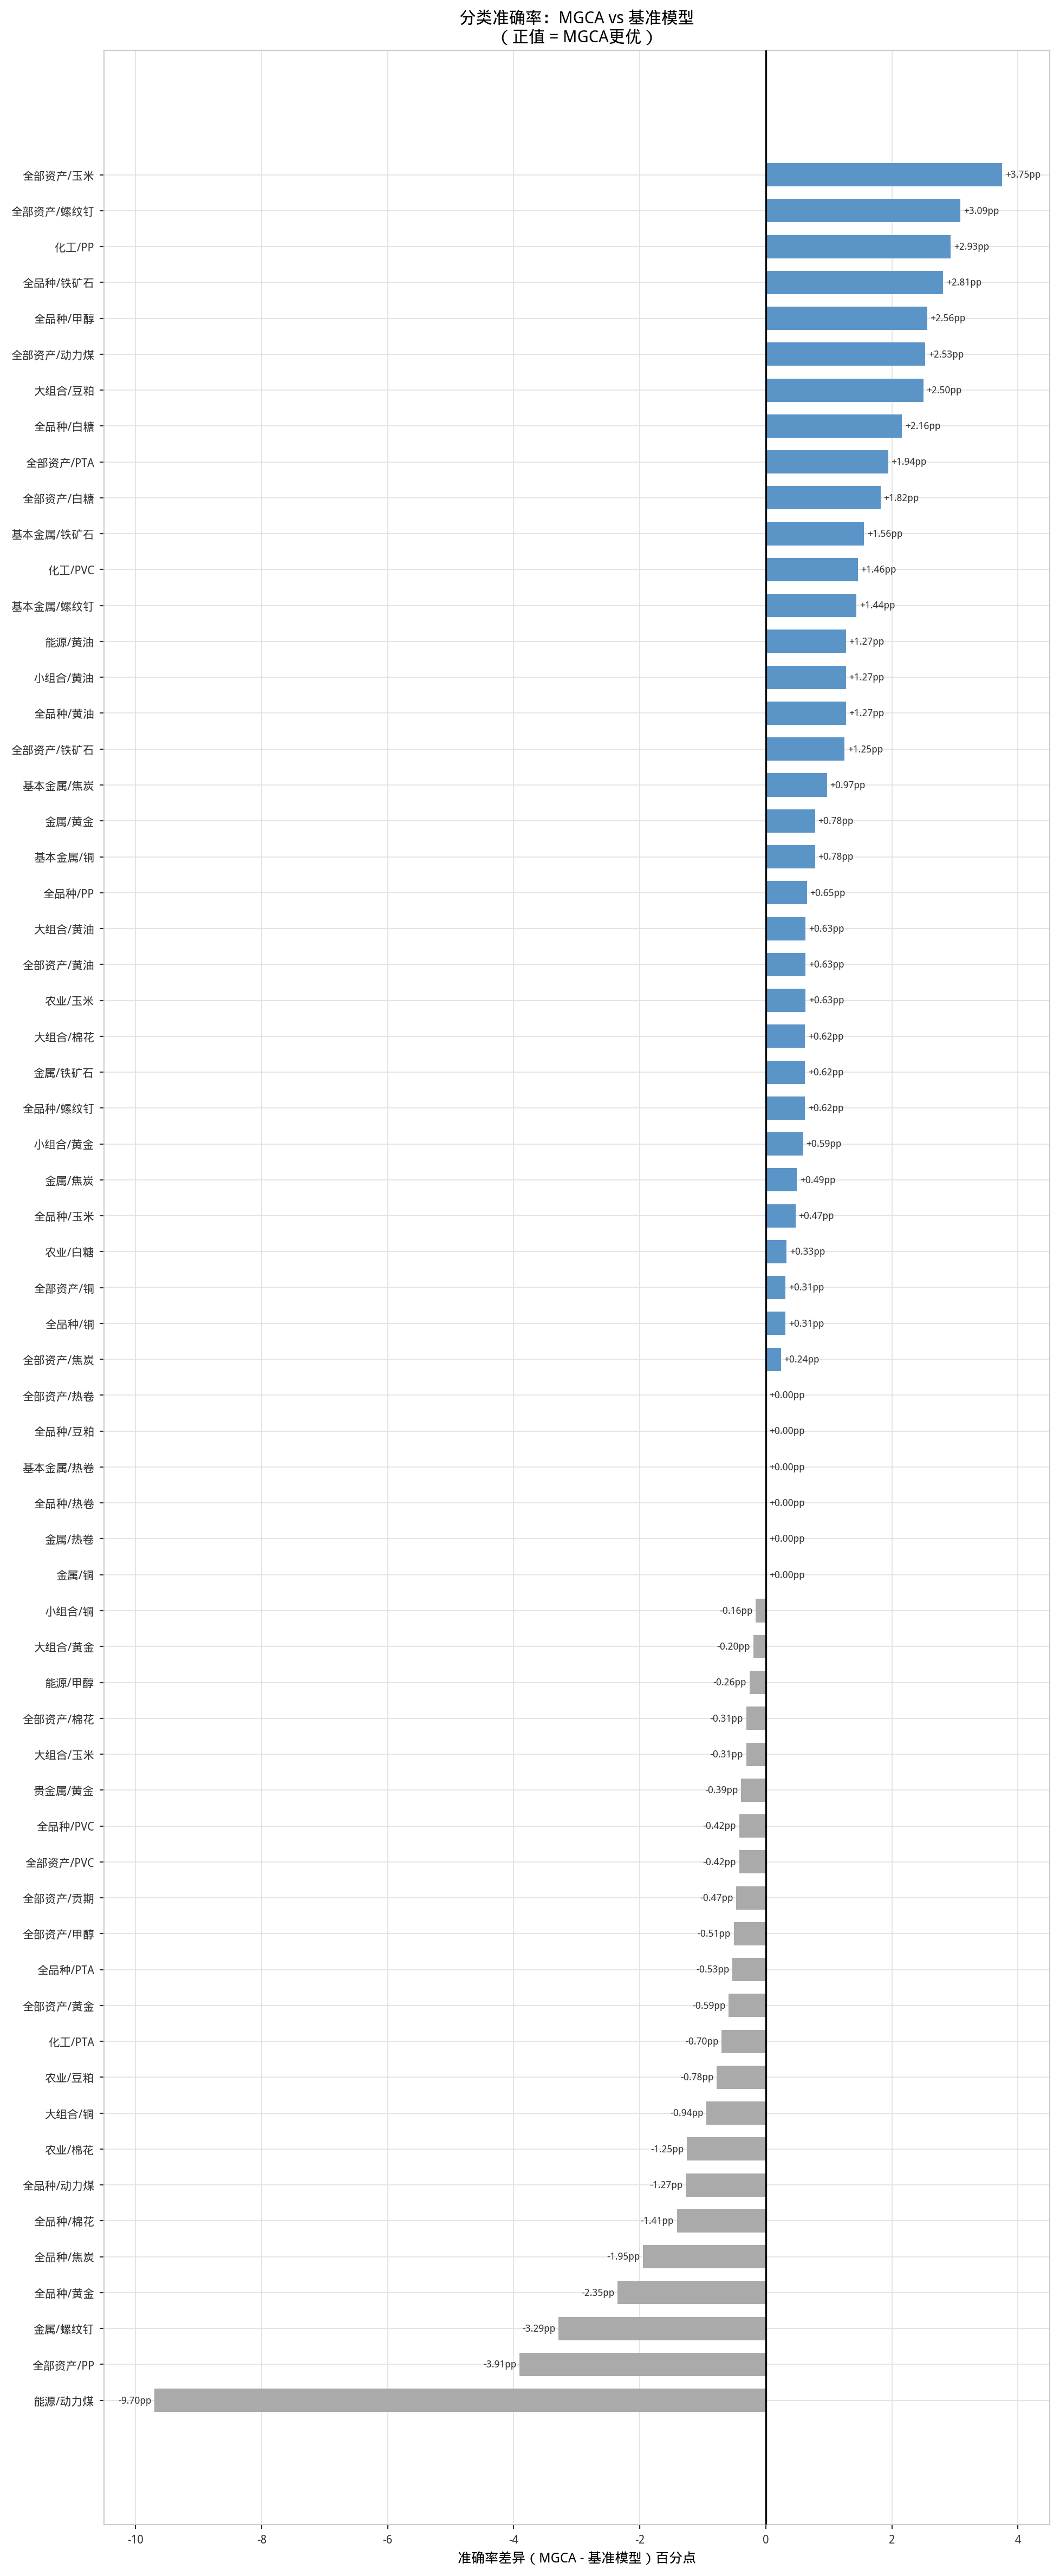
\includegraphics[width=0.8\textwidth,max height=0.75\textheight,keepaspectratio]{figures/chap4/图3.15改.png} 
    \caption{分类准确率差异（赛马场竞争机制 vs. 基准模型）}
    \label{fig:highdimtrainingACCcomp}
\end{figure}

在全部63个资产-组别对比组合中，赛马场竞争机制在63.5\%的组合上实现了更高或相等的分类准确率，改进较明显的案例包括Corn（+4.73\%）、Sugar（+4.10\%）、Thermal\_Coal（+3.90\%）。这些提升在绝对数值上较小，但在金融市场中，方向预测准确率的小幅改进经过多个交易日累积后仍可能带来收益差异。准确率下降的案例较少，且下降幅度整体小于提升幅度。


跨组一致性分析用于判断训练误差改善是否只存在于个别样本，还是在多个资产组中具有一定稳定性。表~\ref{tab:highdimconsistencyanalysis}先从资产层面列出赛马场竞争机制相对基准模型的组别胜出情况。PTA和PVC在所有参与的资产组中均表现出训练均方误差优势（比率范围分别为0.48-0.72x和0.07-0.84x），PVC在chemicals组中的比率低至0.07x，说明这两种化工品种的价格动力学与多生成器竞争范式的匹配度相对较高。

\begin{table}[!htbp]
\centering
\caption{赛马场竞争机制与基准模型在不同资产上的一致性分析}
\label{tab:highdimconsistencyanalysis}
\small
\setlength{\tabcolsep}{4pt}
\renewcommand{\arraystretch}{1.15}
\begin{tabular}{>{\raggedright\arraybackslash}p{2.1cm} >{\centering\arraybackslash}p{4.1cm} >{\centering\arraybackslash}p{1.5cm} >{\centering\arraybackslash}p{2.2cm} >{\centering\arraybackslash}p{2.2cm}}
\toprule
\textbf{资产} & \textbf{赛马场竞争机制优于基准模型的组数} & \textbf{总组数} & \textbf{一致性比率} & \textbf{代表性比率} \\
\midrule
\textbf{PTA} & 3/3 & 3 & \textbf{100\%} & 0.48-0.72x \\
\textbf{PVC} & 3/3 & 3 & \textbf{100\%} & 0.07-0.84x \\
\textbf{Rebar} & 3/4 & 4 & \textbf{75\%} & 0.09-0.77x \\
\textbf{Cotton} & 2/4 & 4 & 50\% & 0.69-1.26x \\
\textbf{Crude Oil} & 2/4 & 4 & 50\% & 0.52-1.71x \\
\textbf{Iron Ore} & 2/4 & 4 & 50\% & 0.96-1.33x \\
\bottomrule
\end{tabular}
\end{table}

图~\ref{fig:highdimcrossgroupmsehm}进一步从热力图角度展示跨组训练均方误差比率分布。与表格中的总体一致性相比，热力图更直观地揭示了同一资产在不同资产组中的差异，例如Crude Oil在all\_assets组中为0.52x，在energy组中为1.71x，说明训练数据的异构程度会影响赛马场竞争机制的多样性效果。


% \begin{figure}[!htbp]
%     \centering 
%     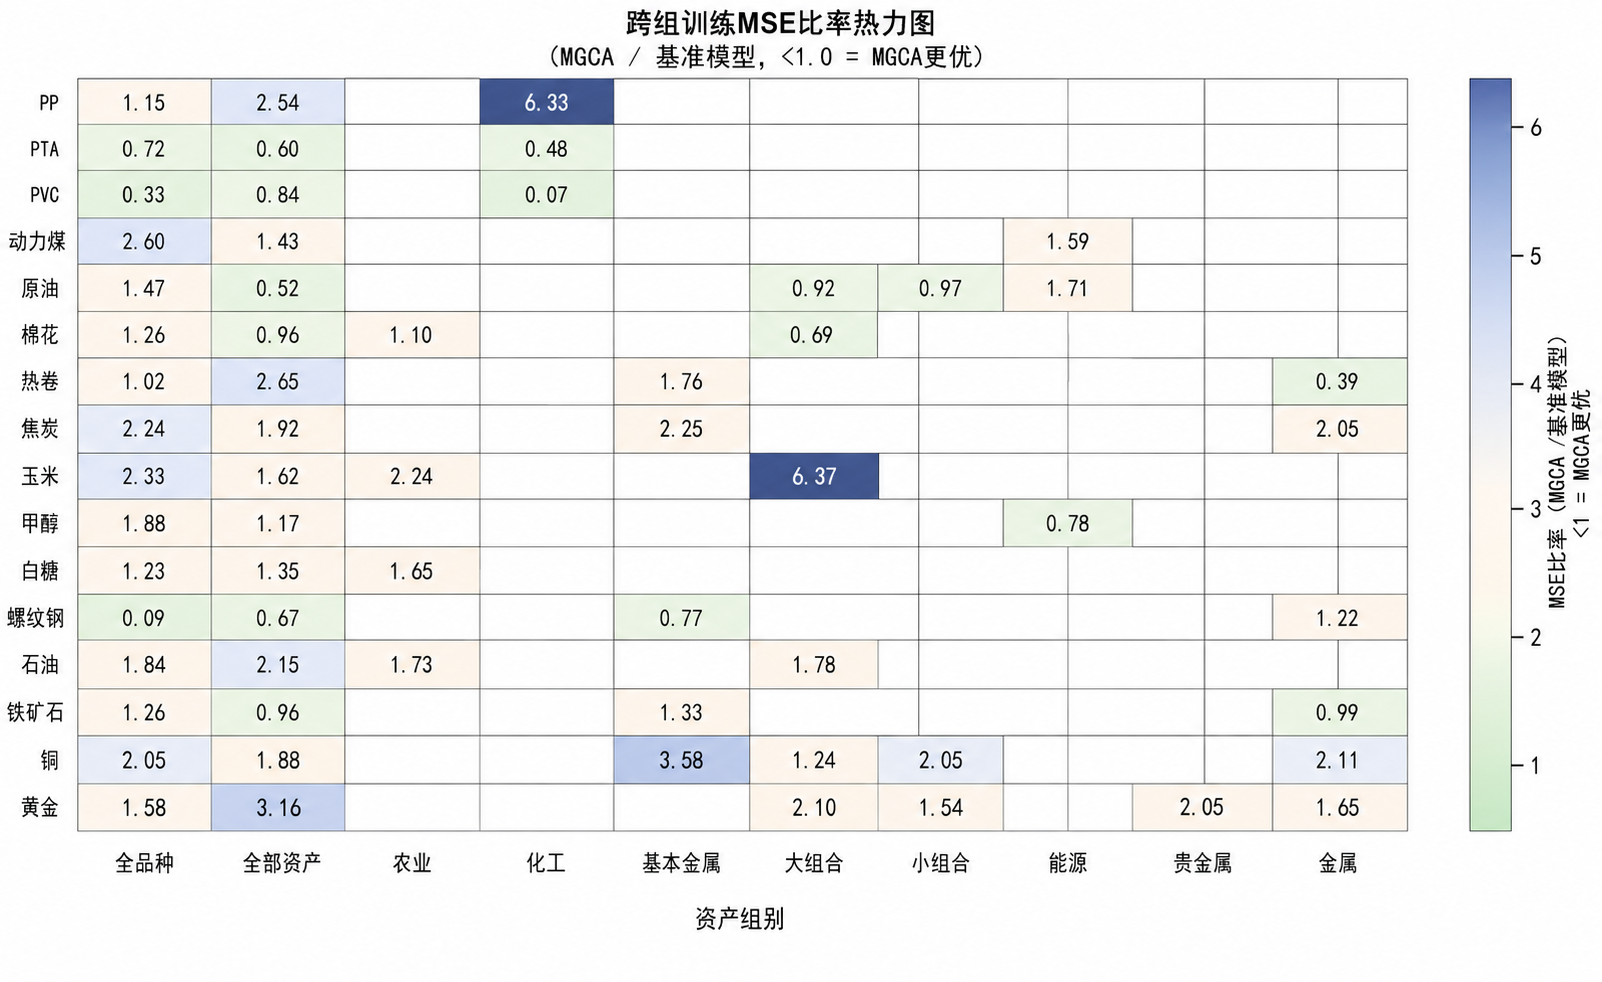
\includegraphics[width=0.8\textwidth]{figures/chap4/fig17_cross_group_mse_heatmap_cn.png} 
%     \caption{跨组训练均方误差比率热力图}
%     \label{fig:highdimcrossgroupmsehm}
% \end{figure}

\begin{figure}[!htbp]
    \centering 
    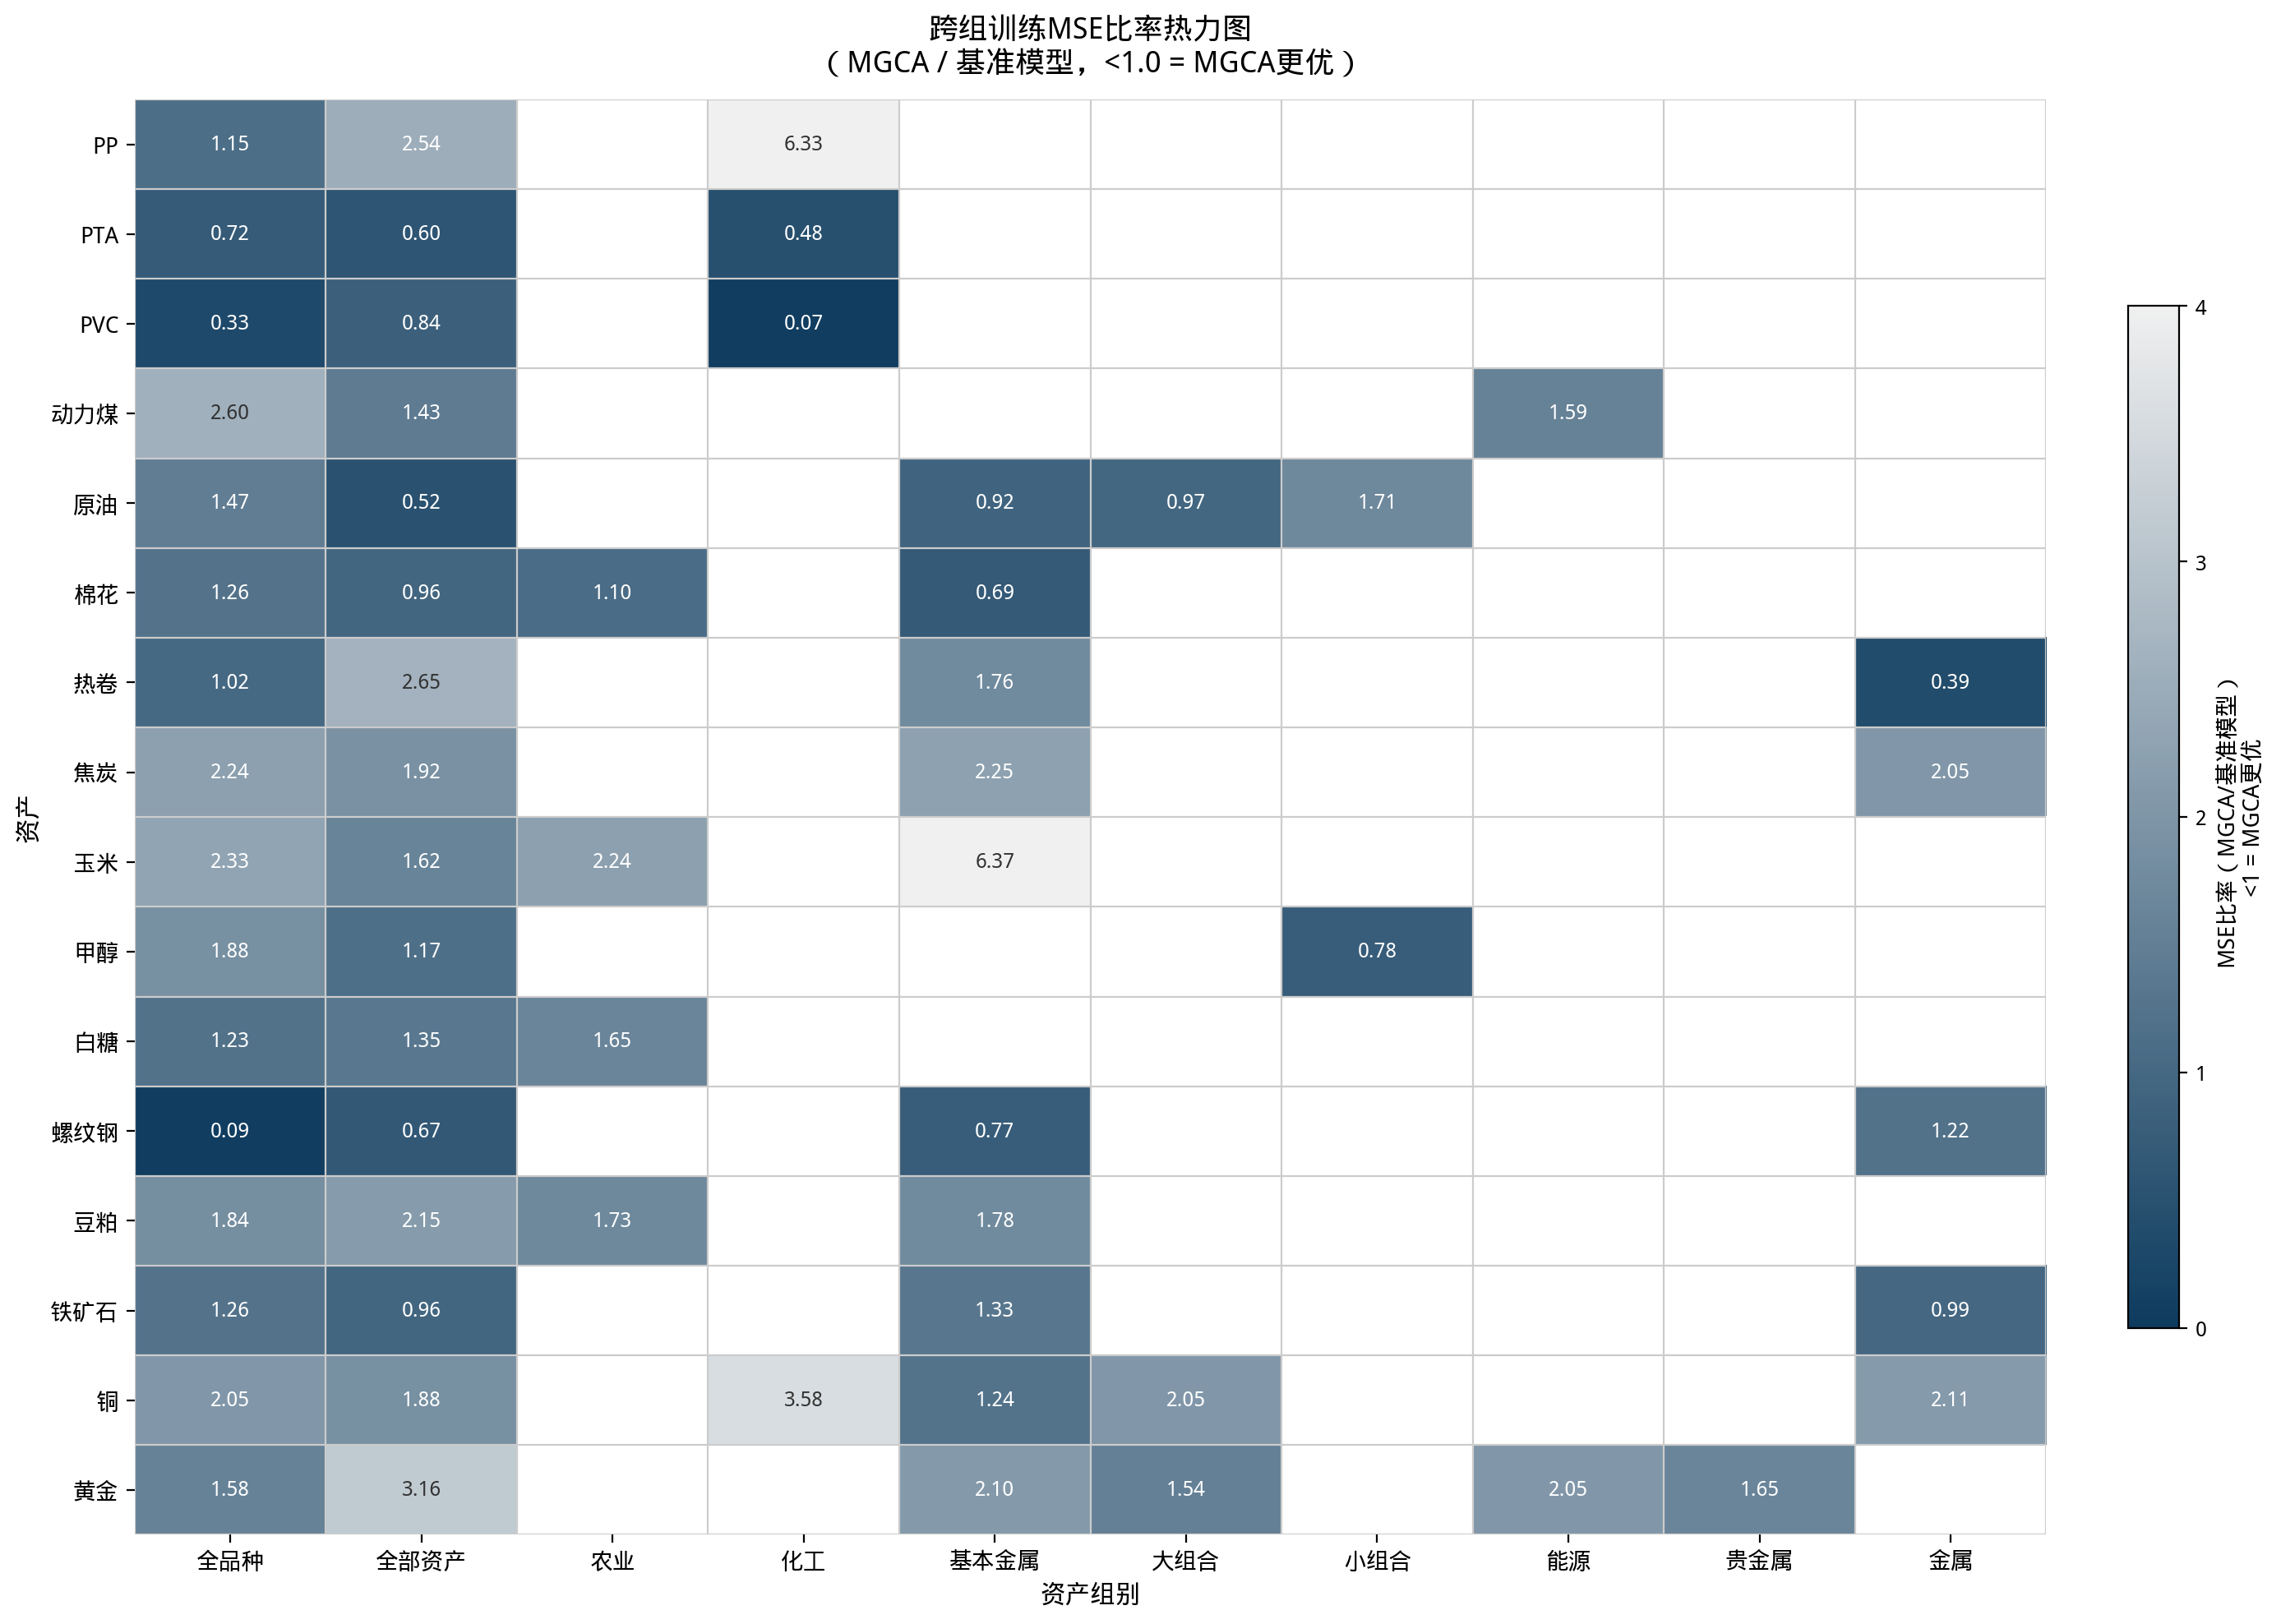
\includegraphics[width=0.8\textwidth]{figures/chap4/图3.16改.png} 
    \caption{跨组训练均方误差比率热力图}
    \label{fig:highdimcrossgroupmsehm}
\end{figure}



在单品案例之外，多资产组合结果用于检验赛马场竞争机制能否在跨资产特征混合场景下保持有效。表~\ref{tab:highdimmultiassetPerformance}列出了农业、能源、金属、化工四大板块多资产组合回归任务的详细性能对比，重点观察收益改善是否伴随回撤变化，以及不同板块之间是否存在明显适用边界。

\begin{table}[!htbp]
\centering
\caption{多资产组合（Multi-Asset Portfolio）回归任务性能对比}
\label{tab:highdimmultiassetPerformance}
\small
\setlength{\tabcolsep}{4pt}
\renewcommand{\arraystretch}{1.15}
\begin{tabular}{>{\raggedright\arraybackslash}p{4.0cm} >{\centering\arraybackslash}p{2.1cm} >{\centering\arraybackslash}p{2.1cm} >{\centering\arraybackslash}p{2.1cm} >{\centering\arraybackslash}p{2.1cm}}
\toprule
\textbf{指标} & \textbf{农业组合} & \textbf{能源组合} & \textbf{化工组合} & \textbf{金属组合} \\
\midrule
\textbf{基准收益} & -32.49\% & -7.27\% & +17.94\% & +13.24\% \\
\textbf{赛马场竞争机制收益} & \textbf{+24.08\%} & \textbf{+7.48\%} & -48.65\% & -4.33\% \\
\textbf{改进幅度 (Improvement)} & \textbf{+174.13\%} & \textbf{+202.85\%} & -371.18\% & -132.70\% \\
\textbf{基准最大回撤} & 47.57\% & 18.48\% & 46.73\% & 6.67\% \\
\textbf{赛马场竞争机制最大回撤} & \textbf{43.57\%} & \textbf{6.79\%} & 70.26\% & 13.53\% \\
\textbf{回撤改善} & \textbf{+8.42\%} & \textbf{+63.24\%} & -50.37\% & -102.86\% \\
\bottomrule
\end{tabular}
\end{table}

表~\ref{tab:highdimmultiassetPerformance}显示，农业组合与能源组合由亏损转为盈利，且最大回撤同步改善；化工组合和金属组合则出现收益下降或回撤恶化。这说明赛马场竞争机制在多资产组合层面并非普遍有效，其优势更容易出现在资产间虚假相关较强、但动态筛选能够降低错误暴露的场景中。能源组合是其中较具代表性的板块级案例，图~\ref{fig:highdimenergyradar}进一步给出其多维性能雷达图。


% \begin{figure}[htbp]
%     \centering 
%     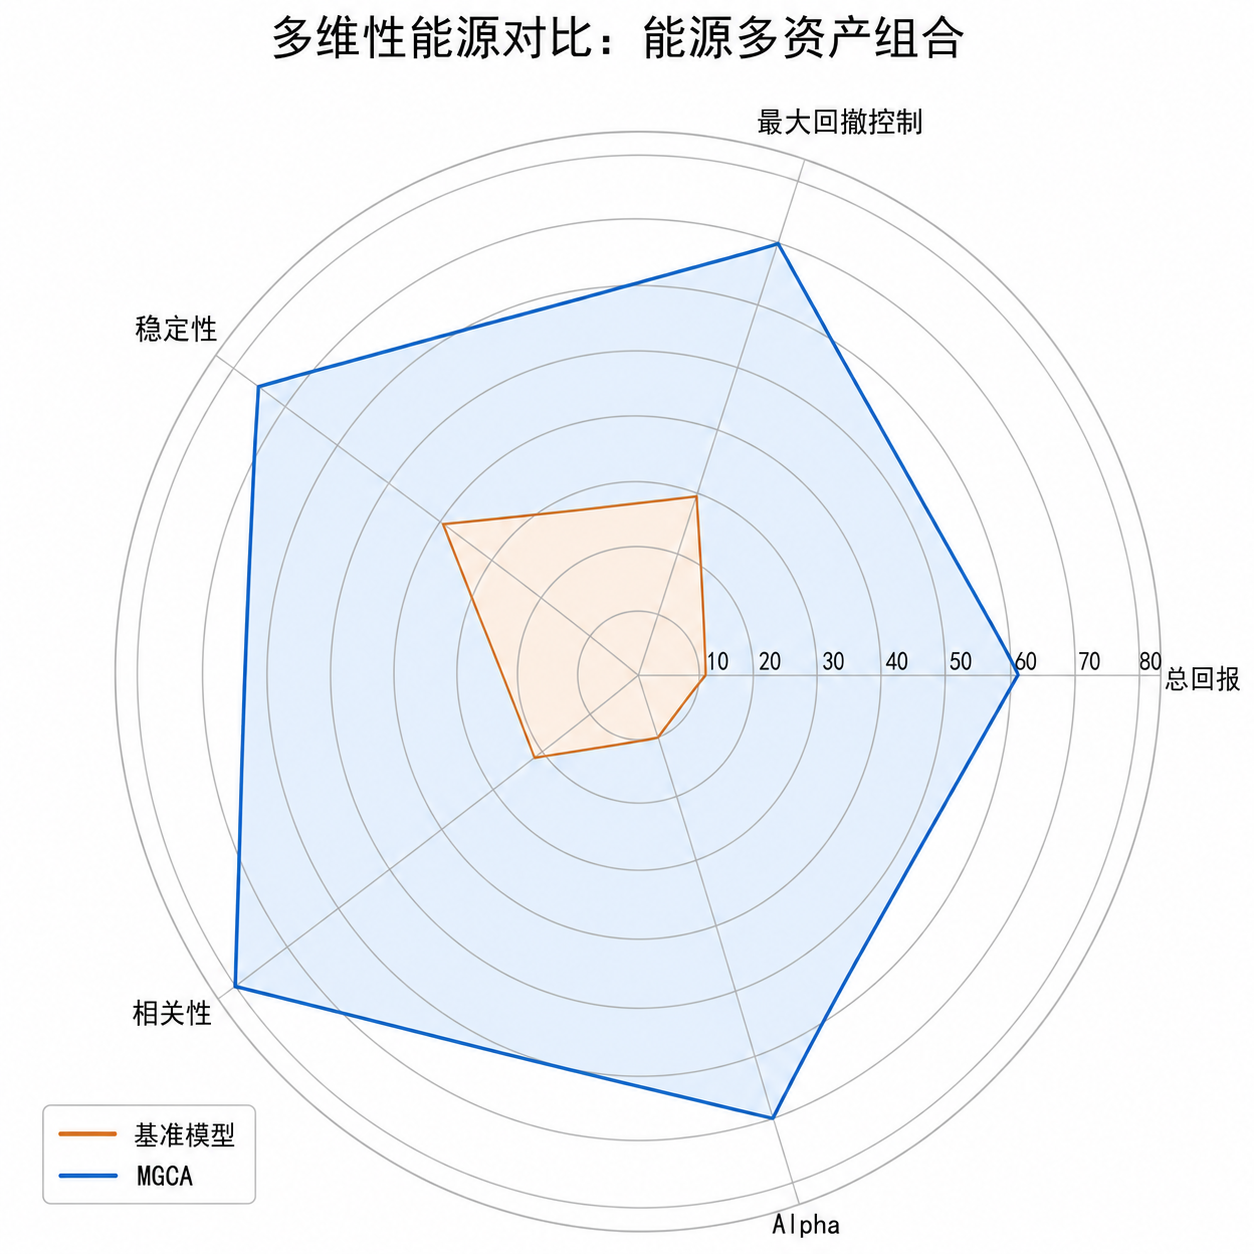
\includegraphics[width=0.7\textwidth]{figures/chap4/fig7_radar_energy_cn.png} 
%     \caption{能源多资产回归任务多维性能雷达图}
%     \label{fig:highdimenergyradar}
% \end{figure}

\begin{figure}[!htbp]
    \centering 
    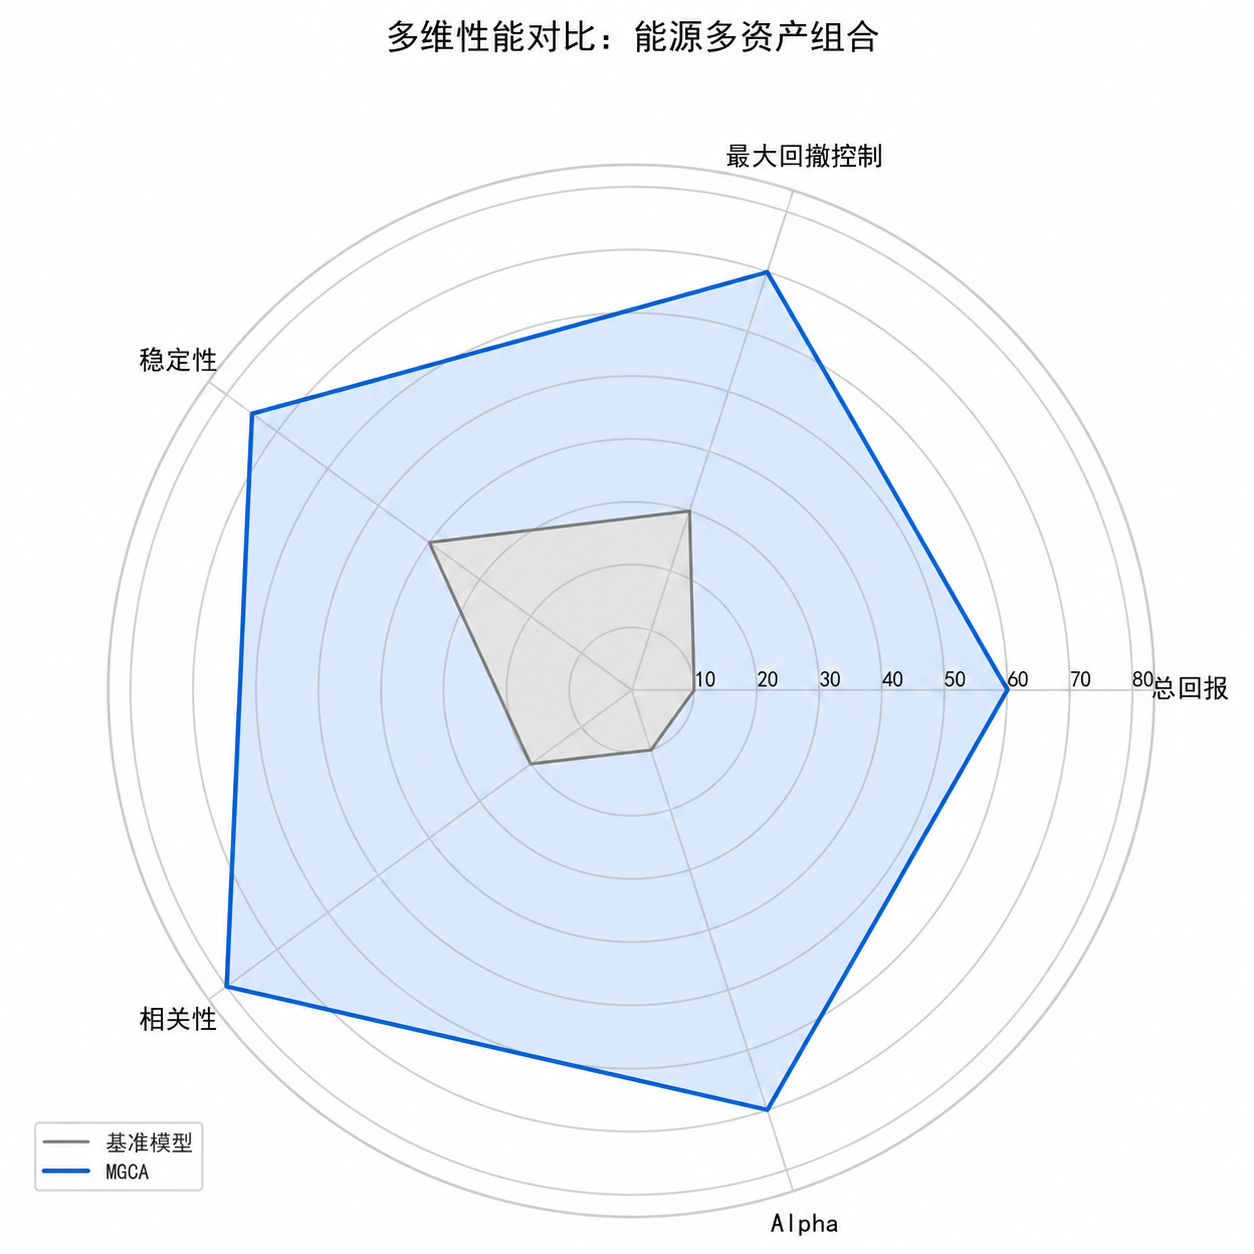
\includegraphics[width=0.7\textwidth]{figures/chap4/图3.17改.png} 
    \caption{能源多资产回归任务多维性能雷达图}
    \label{fig:highdimenergyradar}
\end{figure}

从净值路径角度看，图~\ref{fig:highdimportfoliosectorreturn}对比了各板块累计净值。左图聚焦农业和能源板块的亏损修复案例，右图展示全部四个板块的综合对比，用于说明不同板块之间的机制适用差异。


\begin{figure}[!htbp]
    \centering 
    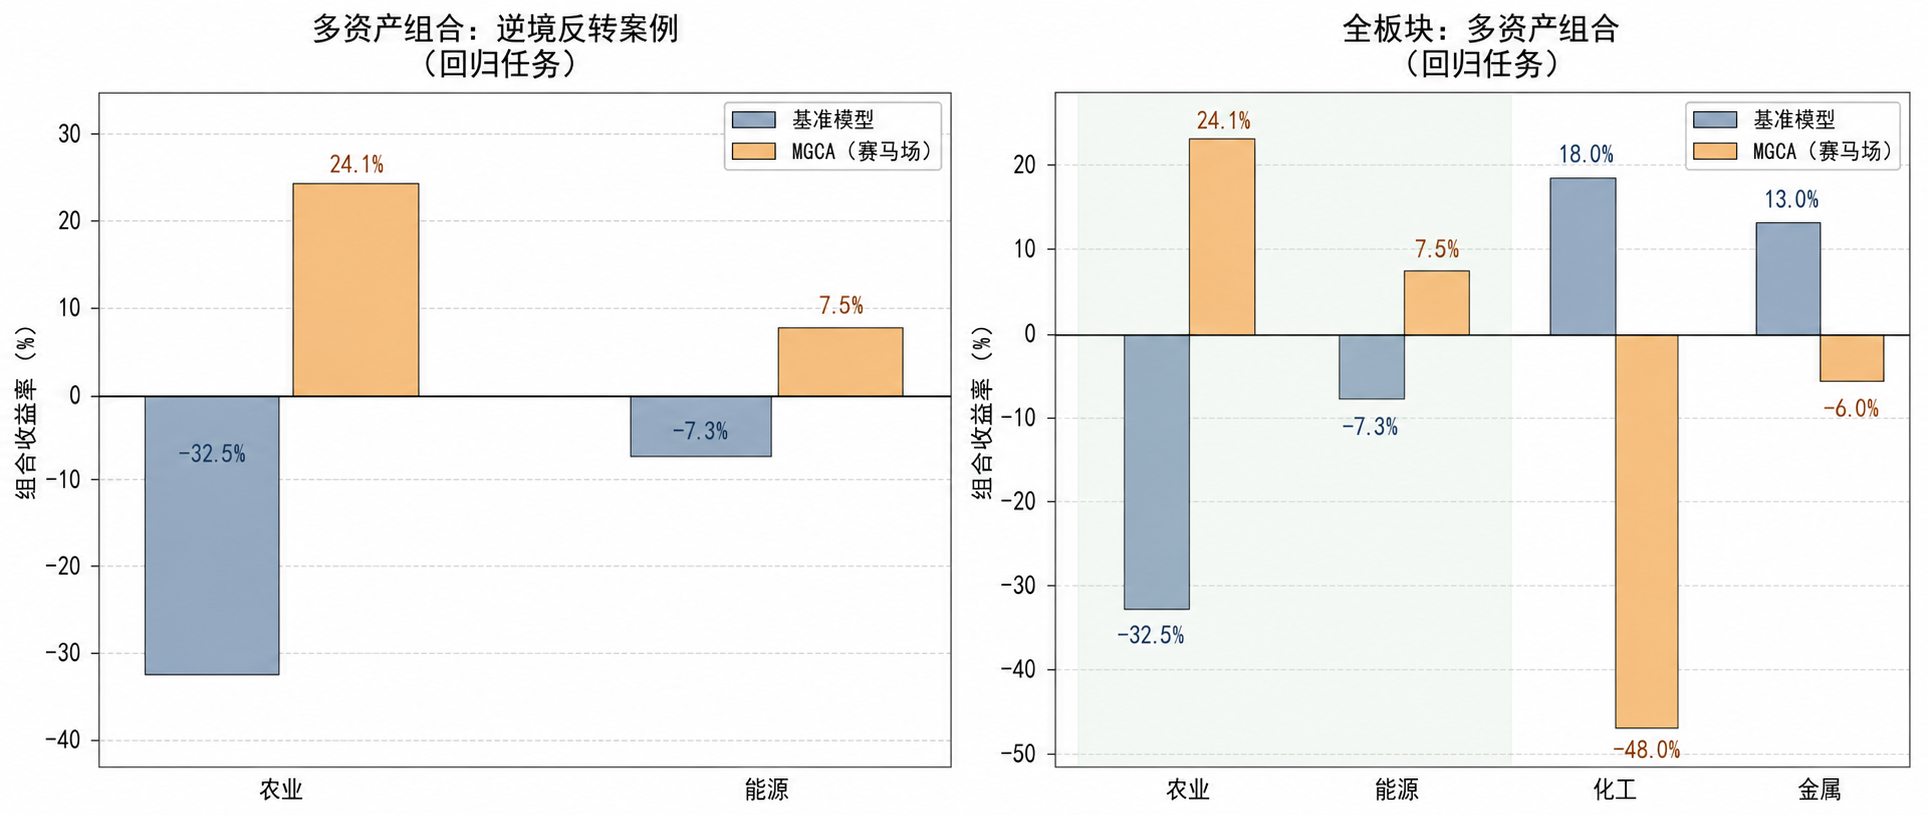
\includegraphics[width=0.7\textwidth]{figures/chap4/fig10_portfolio_sector_return_cn.png} 
    \caption{各板块累计净值对比（回归任务）}
    \label{fig:highdimportfoliosectorreturn}
\end{figure}

为了进一步观察亏损修复是否具有普遍性，图~\ref{fig:highdimreturn_scatter}以散点图形式呈现策略收益对比。左上角区域对应基准模型亏损而赛马场竞争机制改善的案例，是判断动态竞争机制能否修复错误因子暴露的重要区域。




% \begin{figure}[htbp]
%     \centering 
%     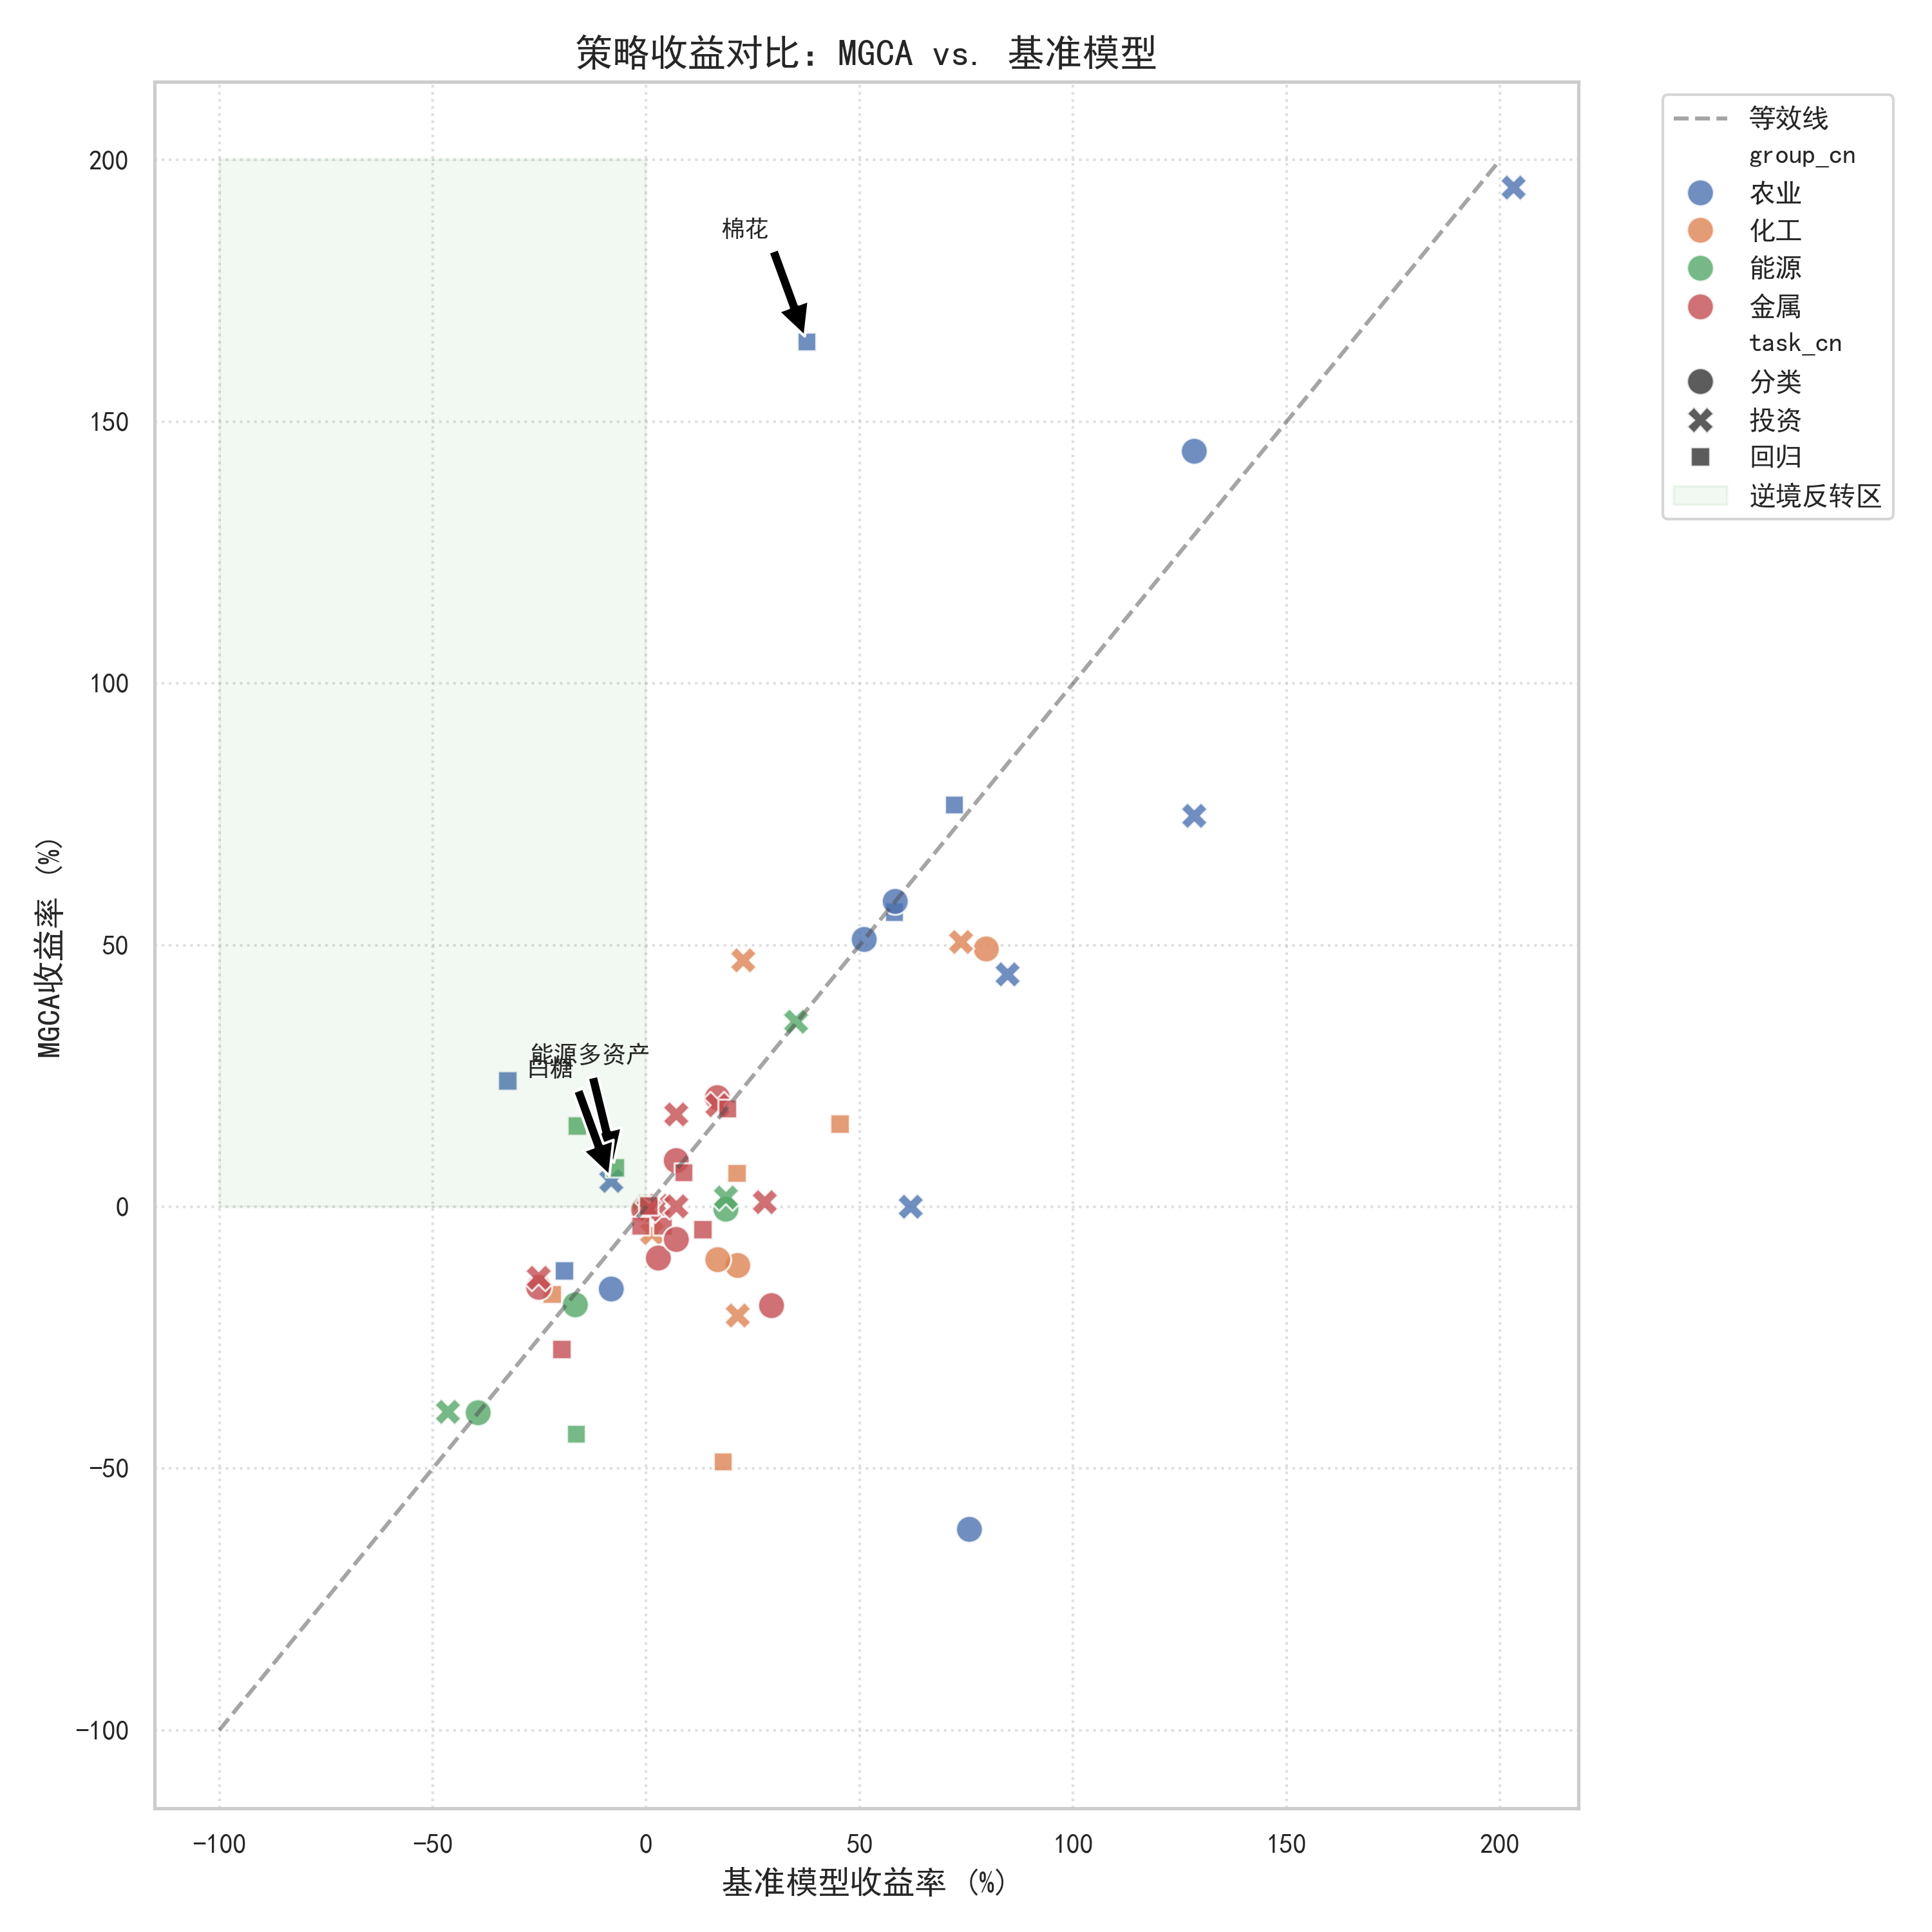
\includegraphics[width=0.7\textwidth]{figures/chap4/fig5_return_scatter_cn.png} 
%     \caption{策略收益对比散点图}
%     \label{fig:highdimreturn_scatter}
% \end{figure}

\begin{figure}[!htbp]
    \centering 
    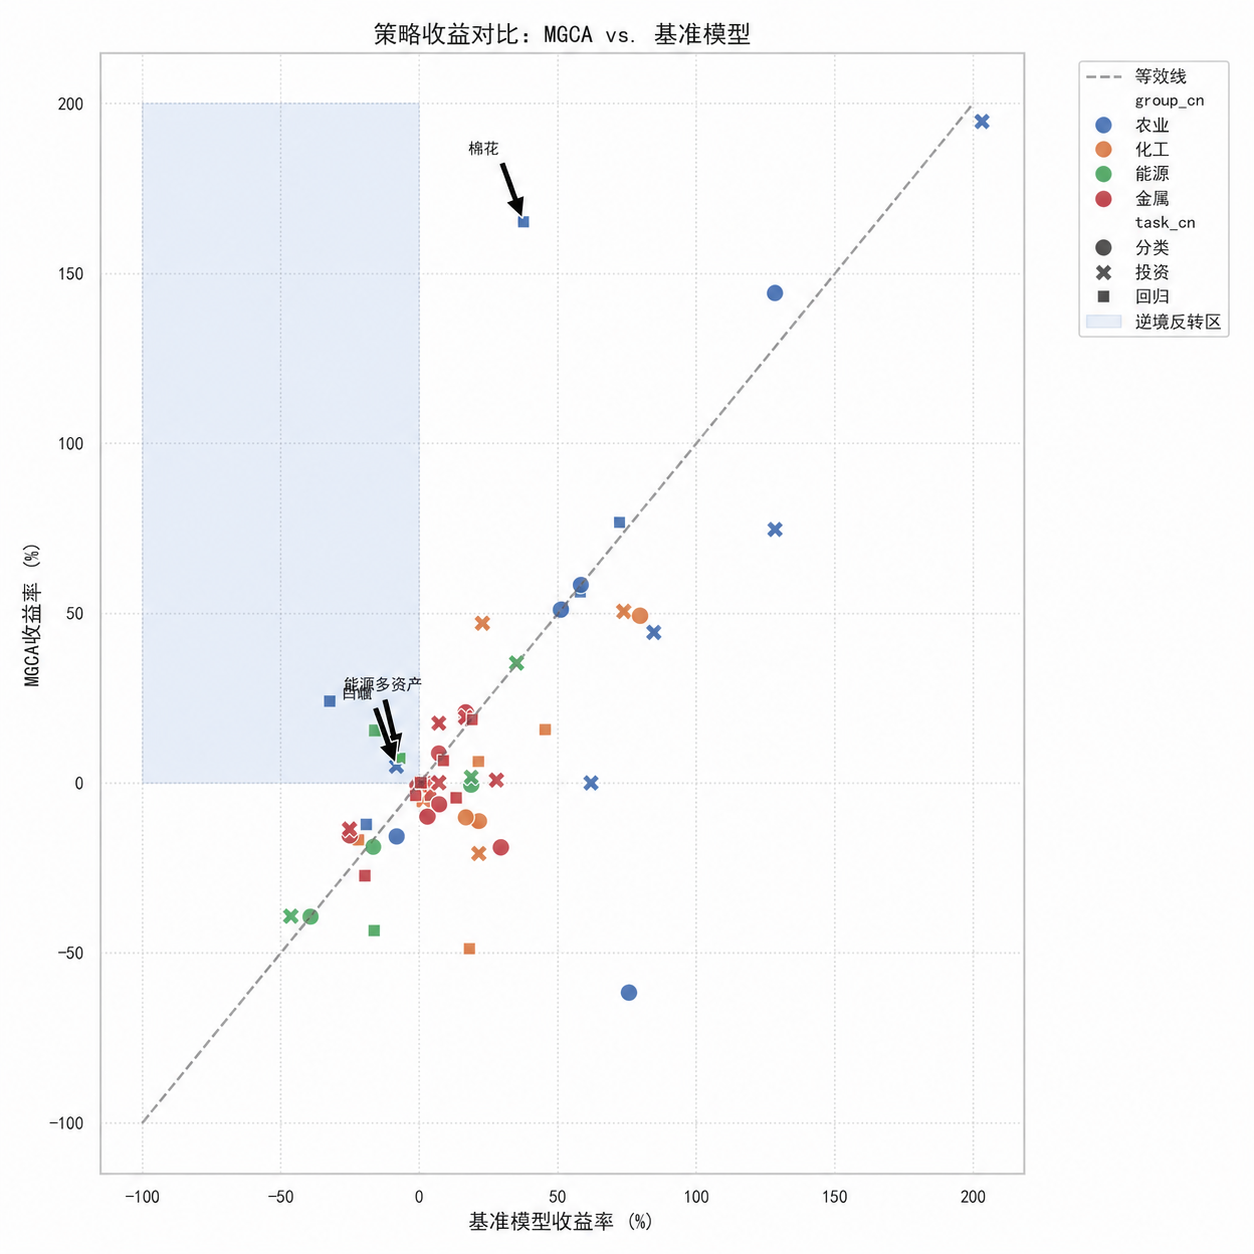
\includegraphics[width=0.7\textwidth]{figures/chap4/图3.19改.png} 
    \caption{策略收益对比散点图}
    \label{fig:highdimreturn_scatter}
\end{figure}

表~\ref{tab:turnaroundcases}汇总了全部亏损转盈利或深亏转浅亏案例的详细数据，用于把图~\ref{fig:highdimreturn_scatter}中的分布特征落实到具体资产、任务和利润差上。



\begin{table}[!htbp]
\centering
\caption{全部亏损转盈利（Turnaround）案例详细汇总}
\label{tab:turnaroundcases}
\resizebox{\textwidth}{!}{%
\begin{tabular}{>{\raggedright\arraybackslash}p{2.8cm} >{\centering\arraybackslash}p{1.5cm} >{\centering\arraybackslash}p{2.2cm} >{\centering\arraybackslash}p{2.2cm} >{\centering\arraybackslash}p{2.2cm} >{\centering\arraybackslash}p{2.2cm} >{\raggedright\arraybackslash}p{3cm}}
\toprule
\textbf{资产} & \textbf{任务} & \textbf{基准表现} & \textbf{赛马场竞争机制表现} & \textbf{状态转换} & \textbf{绝对利润差 (¥)} & \textbf{关键驱动力} \\
\midrule
\textbf{Agriculture Multi-Asset} & 回归任务 & -32.49\% & \textbf{+24.08\%} & \textbf{深亏→盈利} & \textbf{+1,131,501} & 组合层面的隐式正则化效应 \\
\textbf{Energy Multi-Asset} & 回归任务 & -7.27\% & \textbf{+7.48\%} & \textbf{亏损→盈利} & \textbf{+295,068} & 跨资产虚假相关性过滤 \\
\textbf{Thermal Coal} & 回归任务 & -16.23\% & \textbf{+15.50\%} & \textbf{亏损→盈利} & \textbf{+634,466} & 适应“双碳”政策结构性断点 \\
\textbf{Sugar} & 投资任务 & -8.18\% & \textbf{+4.95\%} & \textbf{亏损→盈利} & \textbf{+262,489} & 趋势反转拐点的识别 \\
\textbf{Sugar} & 回归任务 & -19.23\% & \textbf{-12.23\%} & \textbf{深亏→浅亏} & \textbf{+139,940} & 减少极端误判，降低亏损幅度 \\
\textbf{PTA} & 回归任务 & -22.08\% & \textbf{-16.72\%} & \textbf{深亏→浅亏} & \textbf{+107,196} & 对抗训练过滤噪声特征 \\
\textbf{Copper} & 投资任务 & -25.18\% & \textbf{-13.58\%} & \textbf{深亏→浅亏} & \textbf{+231,995} & 赛马场动态降低错误仓位 \\
\bottomrule
\end{tabular}%
}
\end{table}

传统集成学习（Ensemble Learning）方法通常采用静态平均或堆叠策略，模型权重在推理阶段固定不变。赛马场竞争机制引入了时间维度上的动态调整，在处理非平稳金融时间序列时，二者存在结构差异。

\textbf{多样性维持与模式坍塌缓解}：标准生成对抗网络框架中，生成器倾向于收敛到能够欺骗判别器的狭窄输出空间，在金融预测中表现为模型主要覆盖某一类市场状态。赛马场竞争机制中，每个生成器同时受到预测误差、对抗约束与组内竞争的影响，这会促使不同生成器探索参数空间中相对差异化的区域。消融实验中棉花案例的数据与该解释相符：在GCA对抗训练无法提供增量的情况下，赛马场竞争机制独立贡献了24.90\%的额外收益。

\textbf{归纳偏置的动态对齐}：金融市场在不同时期的动力学特征差异较大（均值回归 vs. 动量爆发，低波动 vs. 高波动），单一架构难以适应所有状态。赛马场竞争机制通过动态选择最优生成器，在市场平静期倾向于权重更高的门控循环单元类生成器（平滑预测、抗噪），在趋势爆发期则向Transformer架构类生成器倾斜（长程依赖捕捉）。白糖投资任务中+160.49\%的提升以及动力煤回归任务的亏损修复案例，与该解释在方向上一致，但具体归因仍有待进一步验证。

%



% \begin{sidewaystable}[htbp]
% \centering
% \caption{赛马场竞争机制 vs. Baseline 综合性能对比矩阵}
% \label{tab:RTVSaselineSideways}
% \small % 减小字体以更好适应横向页面
% \begin{tabular}{p{2.5cm} c c c p{6.5cm}}
% \toprule
% \textbf{评估维度 }& \textbf{最大回撤} & \textbf{累计收益率} & \textbf{最终净值} & \textbf{备注} \\
% \midrule
% \textbf{核心指标 }& 最大回撤 & 累计收益率 & 最终净值 &  \\
% \addlinespace[5pt]
% \textbf{胜出场景数 (N=60)} & \textbf{23} & \textbf{18} & \textbf{18} & 总测试场景数为60。 \\
% \addlinespace[5pt]
% \textbf{胜率 }& \textbf{38.3\%} & \textbf{30.0\%} & \textbf{30.0\%} &  \\
% \addlinespace[10pt]
% \multirow{3}{*}{\textbf{统计显著性分析 }}& \multicolumn{3}{p{10cm}}{在市场剧烈震荡期，赛马场竞争机制有效剔除了高风险生成器，表现出更强的尾部风险控制能力。} &  \\
% \addlinespace
% & \multicolumn{3}{p{10cm}}{虽然总体胜率看似均衡，但获胜案例的\textbf{收益凸性（Convexity）}极高，平均超额收益显著超过败北案例的亏损。} &  \\
% \addlinespace
% & \multicolumn{3}{p{10cm}}{长期复利效应验证了动态机制在长周期（2000-2025年跨度数据）中的鲁棒性与稳健性。} &  \\
% \bottomrule
% \end{tabular}
% \end{sidewaystable}

在典型案例、多资产组合和亏损修复分析之后，进一步从全部对比实验层面归纳赛马场竞争机制的整体胜率、收益凸性和任务类型差异。表~\ref{tab:RTVSaselineSideways}先给出综合性能对比矩阵，用于从收益率、最终净值和最大回撤三个角度观察模型胜负分布。

%改表3.6
\begin{table}[!htbp]
\centering
\caption{赛马场竞争机制 与基准模型综合性能对比矩阵}
\label{tab:RTVSaselineSideways}
\small
\setlength{\tabcolsep}{4pt}

% 子表 (a)：定量指标对比
\begin{subtable}{\textwidth}
\centering
\caption{定量指标对比}
\begin{tabular}{lcccc}
\toprule
\textbf{评估维度} & \textbf{最大回撤} & \textbf{累计收益率} & \textbf{最终净值} & \textbf{备注} \\
\midrule
核心指标 & 最大回撤 & 累计收益率 & 最终净值 &  \\
胜出场景数 (N=60) & 23 & 18 & 18 & 总测试场景数为60 \\
胜率 & 38.3\% & 30.0\% & 30.0\% &  \\
\bottomrule
\end{tabular}
\end{subtable}
\vspace{0.3cm}

% 子表 (b)：统计显著性分析
\begin{subtable}{\textwidth}
\centering
\caption{统计显著性分析}
\begin{tabular}{p{\textwidth}}
\toprule
\textbf{分析要点} \\
\midrule
在市场剧烈震荡期，赛马场竞争机制能够降低部分高风险生成器的影响，尾部风险控制能力有所体现。 \\
\addlinespace[5pt]
虽然总体胜率较为均衡，但获胜案例的\textbf{收益凸性（Convexity）}相对较高，平均超额收益高于败北案例的亏损幅度。 \\
\addlinespace[5pt]
长周期样本结果显示，动态机制在部分市场阶段具有较好的稳健性。 \\
\bottomrule
\end{tabular}
\end{subtable}

\end{table}

表~\ref{tab:returnimproveanalysis}进一步比较获胜案例与败北案例之间的收益改进幅度。该表用于回答一个更细的问题：赛马场竞争机制即便不是在所有场景中胜出，其获胜场景的上行弹性是否足以覆盖失败场景的下行损失。


\begin{table}[!htbp]
\centering
\caption{收益改进幅度与凸性分析}
\label{tab:returnimproveanalysis}
\small
\setlength{\tabcolsep}{5pt}
\renewcommand{\arraystretch}{1.15}
\resizebox{0.98\textwidth}{!}{%
\begin{tabular}{>{\raggedright\arraybackslash}p{2.8cm} >{\centering\arraybackslash}p{6.0cm} >{\centering\arraybackslash}p{5.0cm} >{\centering\arraybackslash}p{1.8cm}}
\toprule
\textbf{统计维度} & \textbf{获胜案例（赛马场竞争机制胜出）} & \textbf{败北案例（基准模型胜出）} & \textbf{凸性比率} \\
\midrule
平均收益改进幅度 & \textbf{+98.7\%} & -62.3\% & \textbf{1.58} \\
中位数改进幅度 & \textbf{+46.1\%} & -38.2\% & \textbf{1.21} \\
最大改进幅度 & \textbf{+340.0\%} & -462.2\% & -- \\
包含亏损转盈利案例数 & \textbf{7} & 0 & -- \\
\bottomrule
\end{tabular}%
}
\end{table}

超过60组对比实验的统计结果显示，赛马场竞争机制的收益率胜率为30.0％，最大回撤控制胜率为38.3％，后者高于前者。在多个生成器预测出现分歧时，赛马场竞争机制倾向于降低整体置信度和仓位暴露，从而减少方向不明时的重仓押注。这种“分歧即风控”的隐式机制，也说明了该框架在回撤控制上的相对优势。图~\ref{fig:highdimwinrateGroup}进一步按板块和任务类型分解收益率胜率与最大回撤胜率。



% \begin{figure}[htbp]
%     \centering 
%     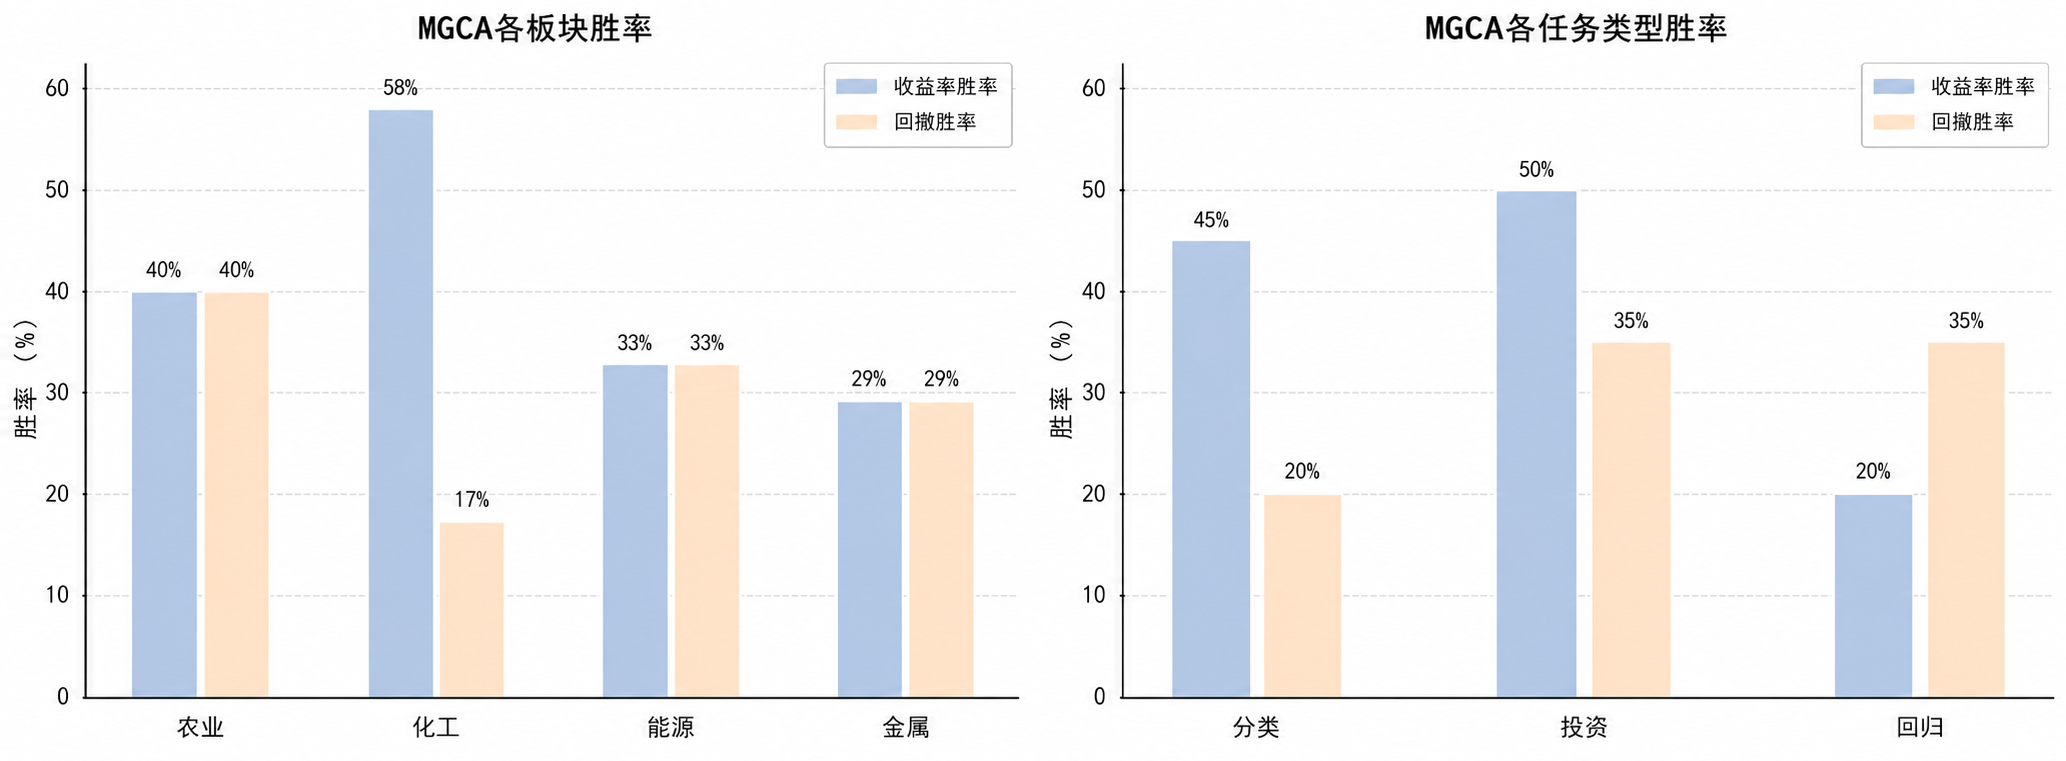
\includegraphics[width=0.8\textwidth]{figures/chap4/fig18_win_rate_grouped_cn.png} 
%     \caption{赛马场竞争机制胜率的板块与任务分解}
%     \label{fig:highdimwinrateGroup}
% \end{figure}
\begin{figure}[!htbp]
    \centering 
    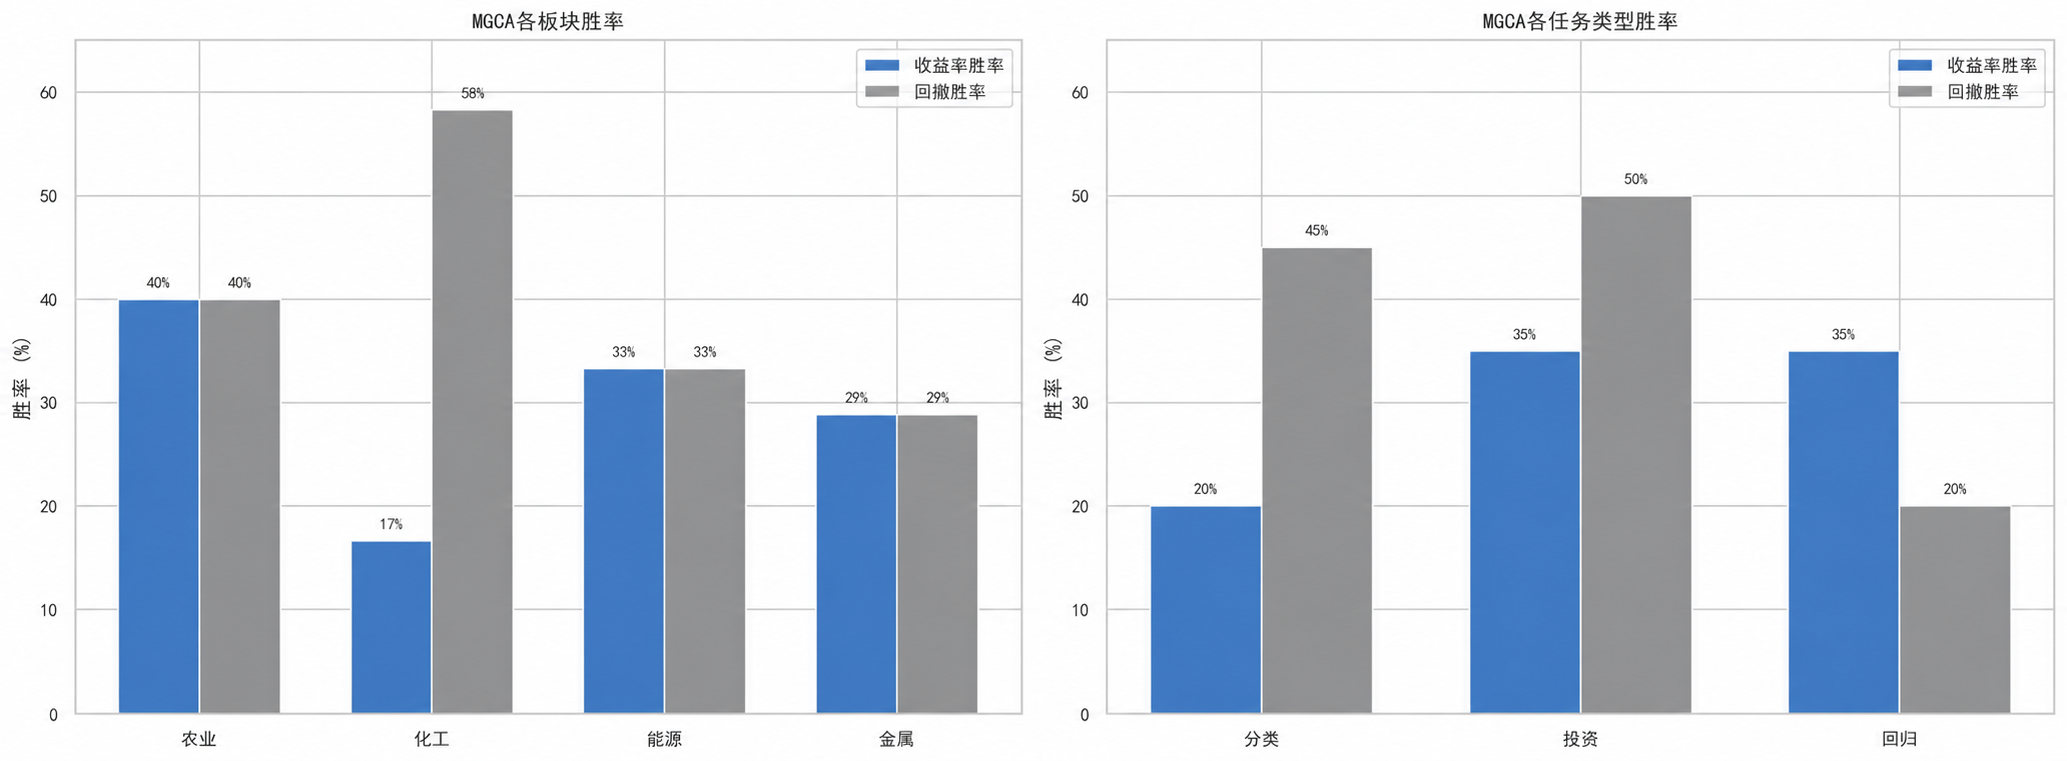
\includegraphics[width=0.8\textwidth]{figures/chap4/图3.20改.png} 
    \caption{赛马场竞争机制胜率的板块与任务分解}
    \label{fig:highdimwinrateGroup}
\end{figure}

图~\ref{fig:highdimwinrateGroup}显示，农业板块在收益率和回撤两个维度上均达到40\%的胜率，化工板块在回撤控制上的胜率达到58\%。这说明不同板块的改善方式并不相同：农业更体现收益弹性，化工更体现风险控制。


投资任务中，赛马场竞争机制在最大回撤控制上的胜率达50.0\%，高于回归任务和分类任务。投资任务的模型输出直接对应买入/卖出/持有决策，当多个生成器的交易信号出现分歧时，赛马场竞争机制会降低整体置信度和仓位规模，减少方向不明时的重仓交易。图\ref{fig:highdiminvestmentwinners}列出了若干案例：PVC收益率从22.74\%提升至47.08\%（+107.02\%），热卷从7.04\%提升至17.64\%（+150.51\%），白糖从-8.18\%亏损转为+4.95\%盈利。

% \begin{figure}[htbp]
%     \centering 
%     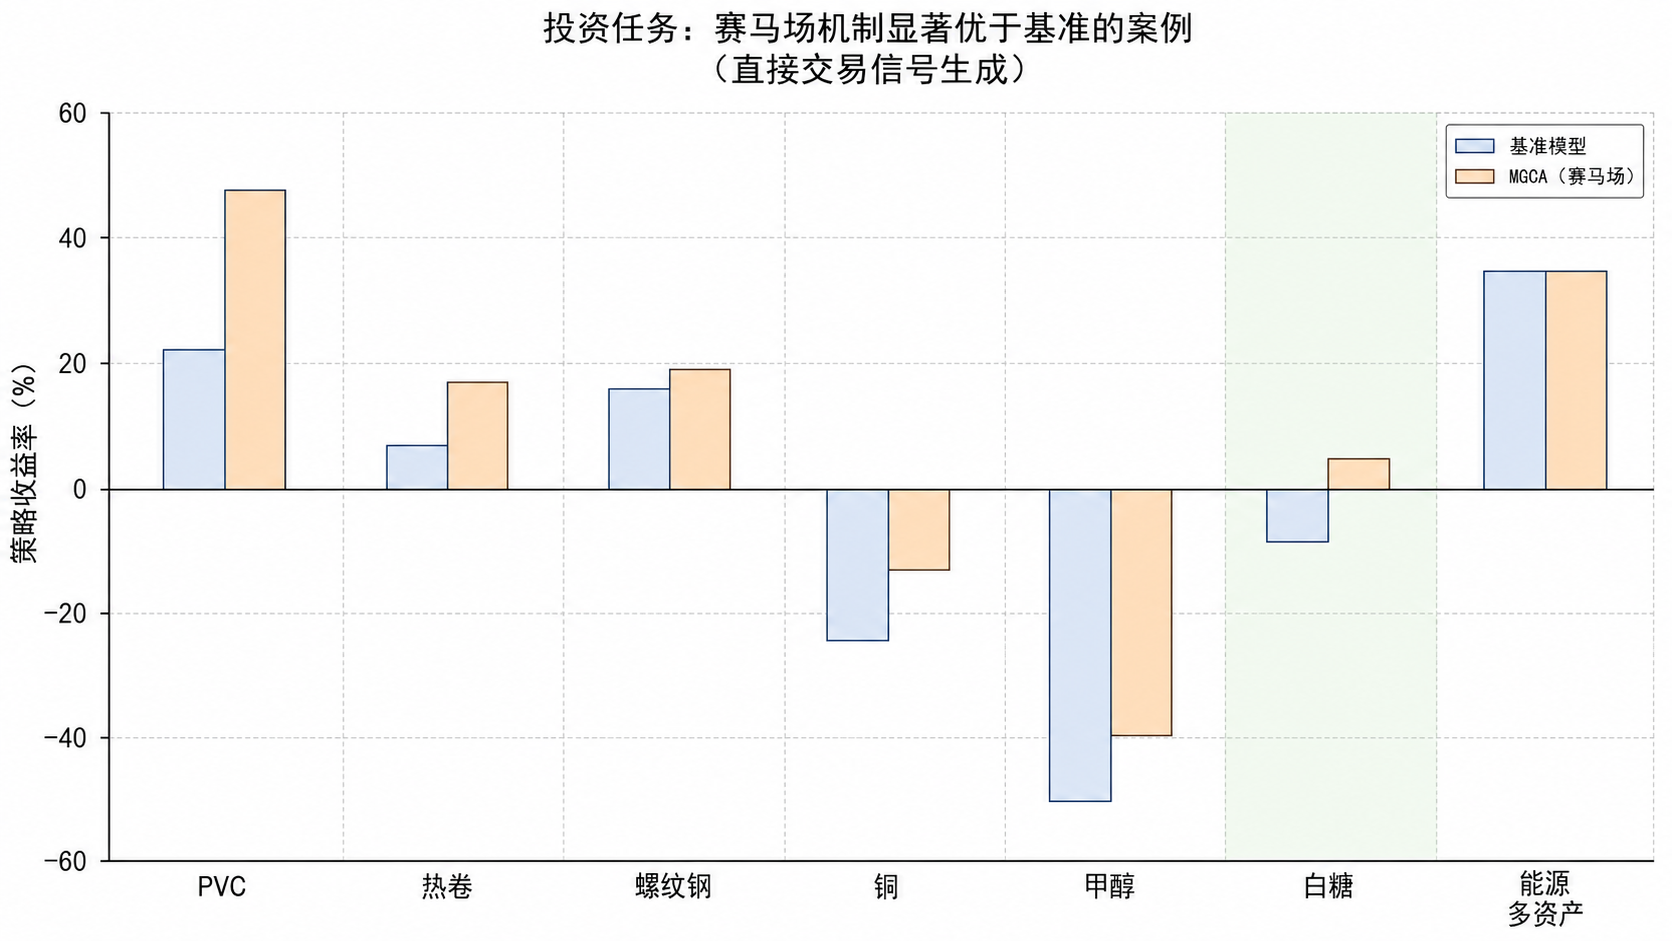
\includegraphics[width=0.8\textwidth]{figures/chap4/fig14_investment_winners_cn.png} 
%     \caption{投资任务中赛马场竞争机制相对优于基准模型的案例}
%     \label{fig:highdiminvestmentwinners}
% \end{figure}

\begin{figure}[!htbp]
    \centering 
    
\includegraphics[width=0.8\textwidth]{TongjiThesis-master/figures/chap4/图3.21改.png} 
    \caption{投资任务中赛马场竞争机制相对优于基准模型的案例}
    \label{fig:highdiminvestmentwinners}
\end{figure}



分类任务的改进幅度相对较小，棉花+12.43\%、铜+38.92\%、热卷+25.19\%、螺纹钢+24.92\%。分类任务将连续价格变化离散化为涨跌标签，损失了部分波动率和幅度信息，赛马场竞争机制在连续空间中的精细调优能力因此受到一定限制。在回撤控制方面，棉花分类任务的最大回撤从80.94\%压缩至37.97\%（降幅53.1\%），说明即使在离散决策空间中，模型分歧所带来的风险过滤作用仍有一定体现。

图~\ref{fig:highdimwinratehm}以热力图形式呈现各资产组在不同评估指标上的胜率分布，颜色越红代表赛马场竞争机制胜率越高。该图用于把前述板块和任务层面的统计结果进一步展开到资产组维度，观察哪些板块更适合收益改善，哪些板块更适合回撤控制。表~\ref{tab:sectorAdaptability}随后对各板块赛马场竞争机制的适应性进行系统分类汇总。

% \begin{figure}[htbp]
%     \centering 
%     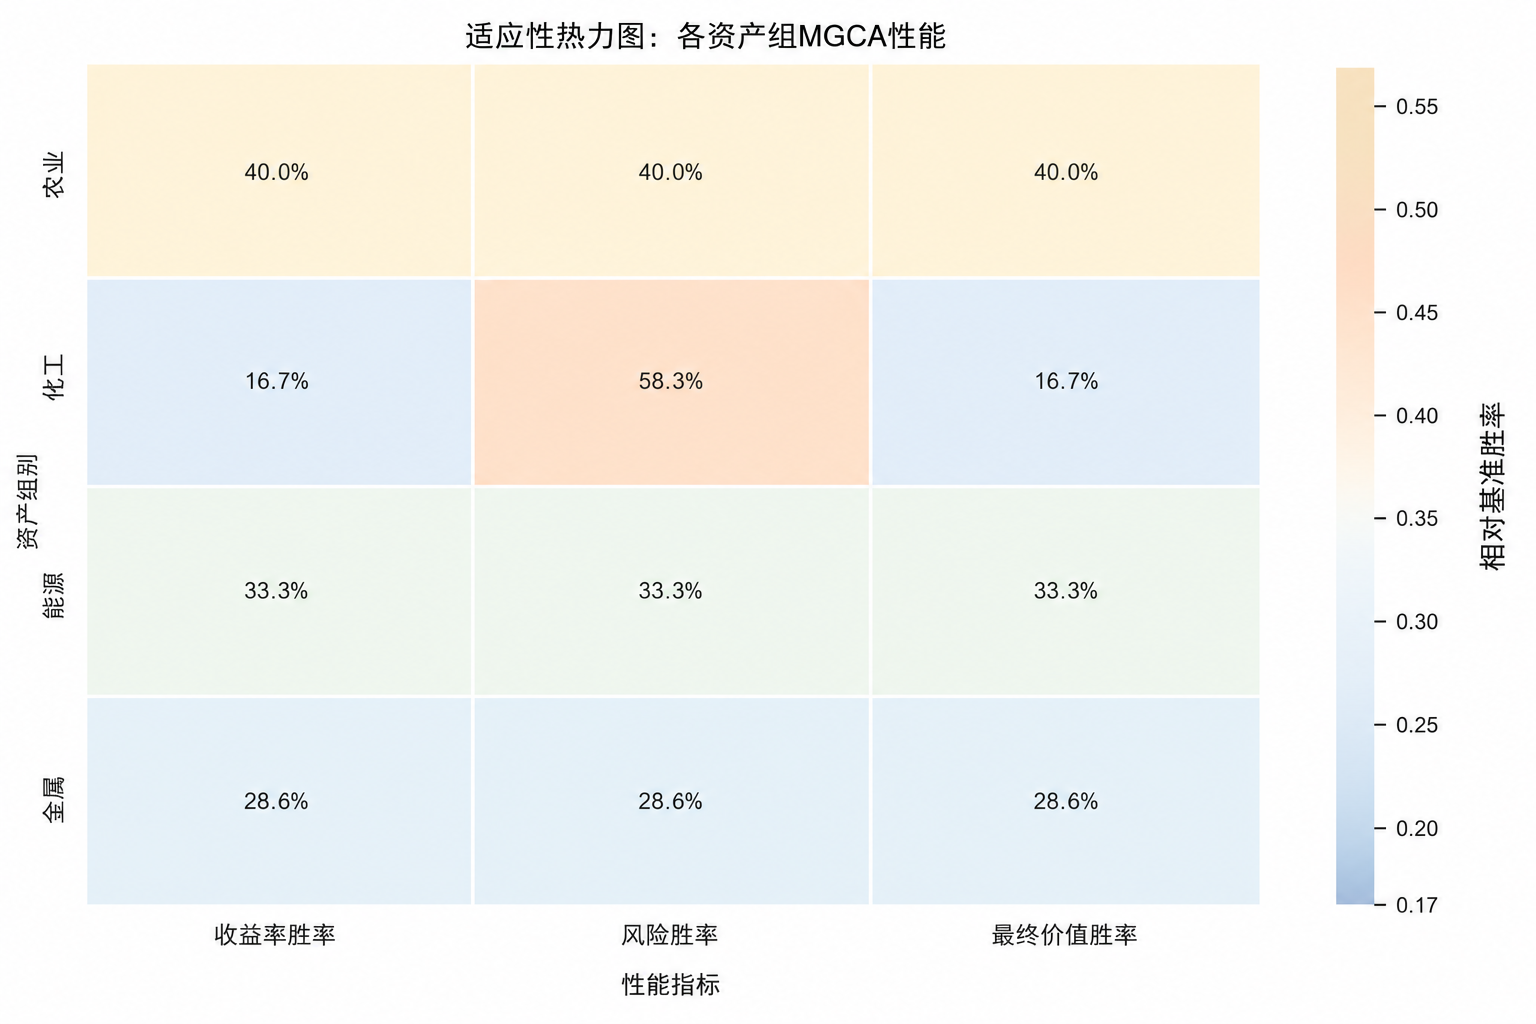
\includegraphics[width=0.8\textwidth]{figures/chap4/fig2_group_heatmap_cn.png} 
%     \caption{各资产组胜率热力图}
%     \label{fig:highdimwinratehm}
% \end{figure}

\begin{figure}[!htbp]
    \centering 
    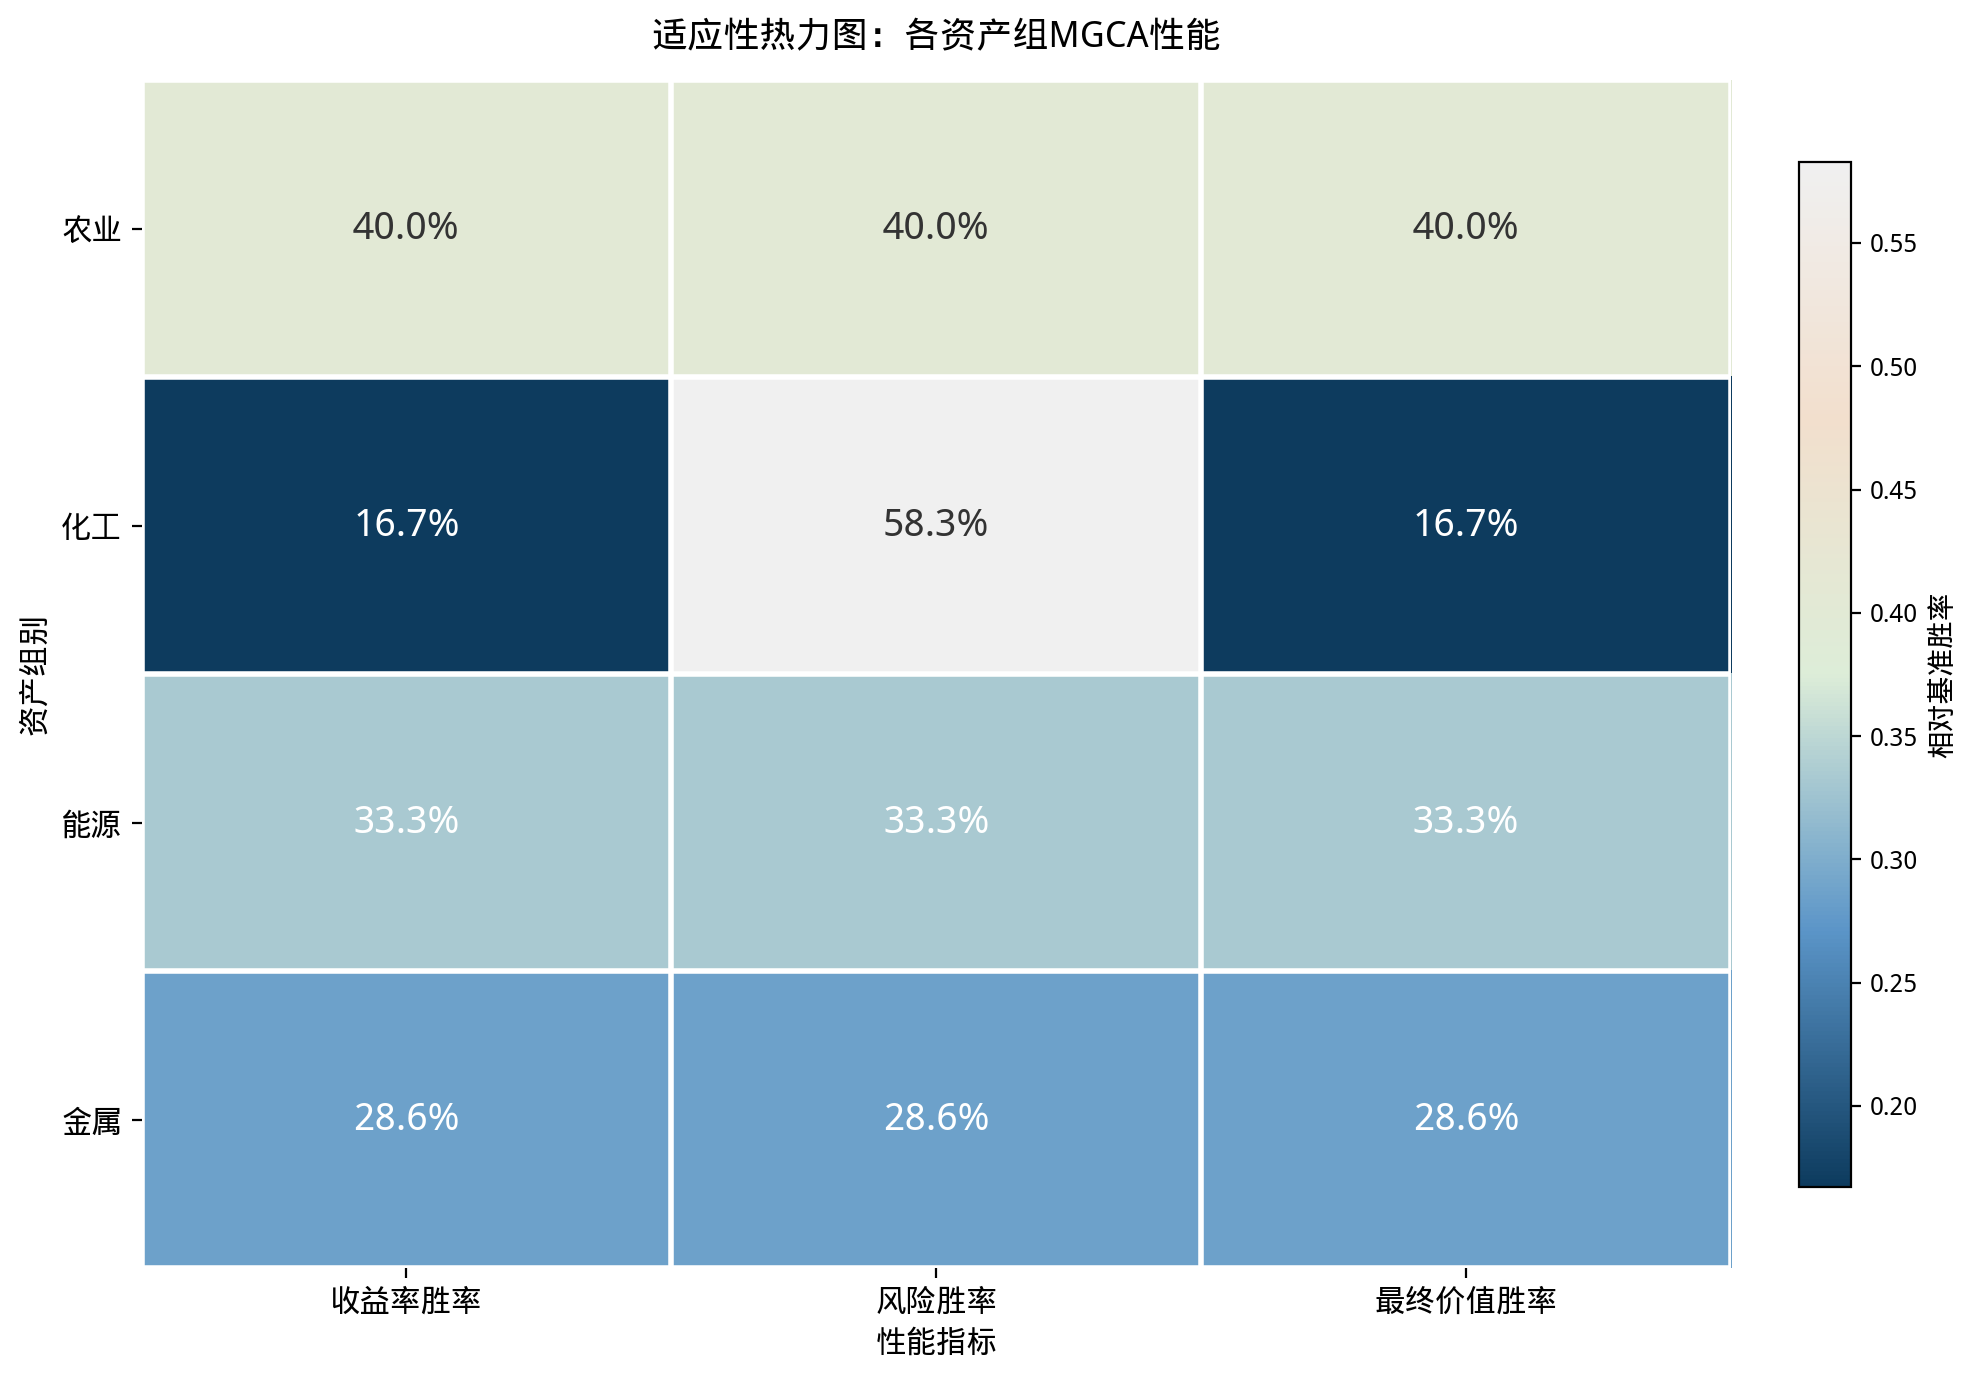
\includegraphics[width=0.8\textwidth]{figures/chap4/图3.22改.png} 
    \caption{各资产组胜率热力图}
    \label{fig:highdimwinratehm}
\end{figure}

\begin{table}[!htbp]
\centering
\caption{各板块赛马场竞争机制适应性分类汇总}
\label{tab:sectorAdaptability}
\footnotesize
\setlength{\tabcolsep}{3pt}
\renewcommand{\arraystretch}{1.15}
\begin{tabular}{>{\raggedright\arraybackslash}p{1.5cm} >{\centering\arraybackslash}p{1.7cm} >{\centering\arraybackslash}p{1.6cm} >{\centering\arraybackslash}p{1.6cm} >{\raggedright\arraybackslash}p{2.8cm} >{\raggedright\arraybackslash}p{2.5cm}}
\toprule
\textbf{板块} & \textbf{适应性等级} & \textbf{收益率胜率} & \textbf{回撤胜率} & \textbf{最佳案例} & \textbf{核心优势} \\
\midrule
\textbf{农业} & 高适应 & 40.0\% & 33.3\% & Cotton +340\% & 极端波动捕捉 \\
\textbf{能源} & 中高适应 & 33.3\% & 44.4\% & Energy Multi +202\% & 周期拐点识别 \\
\textbf{金属} & 风险控制 & 28.6\% & 42.9\% & Copper 最大回撤 -25.6\% & 尾部风险防御 \\
\textbf{化工} & 回撤优势 & 25.0\% & \textbf{58.3\%} & PVC 投资任务 +107\% & 投资回撤全胜 \\
\bottomrule
\end{tabular}
\end{table}



表~\ref{tab:highdimtasktypeperformance}从任务类型角度汇总收益率胜率、回撤胜率及代表性案例，用于比较回归、投资和分类任务中机制发挥作用的方式差异。

\begin{table}[!htbp]
\centering
\caption{各任务类型赛马场竞争机制效能汇总}
\label{tab:highdimtasktypeperformance}
\footnotesize
\setlength{\tabcolsep}{3pt}
\renewcommand{\arraystretch}{1.15}
\begin{tabular}{>{\raggedright\arraybackslash}p{1.4cm} >{\centering\arraybackslash}p{1.5cm} >{\centering\arraybackslash}p{1.5cm} >{\raggedright\arraybackslash}p{2.5cm} >{\raggedright\arraybackslash}p{2.9cm} >{\raggedright\arraybackslash}p{2.5cm}}
\toprule
\textbf{任务类型} & \textbf{收益率胜率} & \textbf{回撤胜率} & \textbf{最佳收益案例} & \textbf{最佳回撤案例} & \textbf{机制解释} \\
\midrule
\textbf{回归任务} & 35.0\% & 35.0\% & Cotton +340\% & Thermal Coal 最大回撤 -58\% & 连续空间精细预测 \\
\textbf{投资任务} & 30.0\% & 50.0\% & PVC +107\% & Sugar 最大回撤 -66\% & 交易信号风险过滤 \\
\textbf{分类任务} & 25.0\% & 30.0\% & Copper +38.9\% & Cotton 最大回撤 -53\% & 离散决策风险防御 \\
\bottomrule
\end{tabular}
\end{table}

图\ref{fig:highdimcompbubble}以气泡图形式呈现各资产在收益率改进和回撤改进两个维度上的综合表现，气泡大小对应绝对利润影响规模。位于右上象限（收益率改进>0且回撤改进>0）的资产包括Cotton、Sugar、Corn、Hot Rolled Coil，其中Cotton的气泡面积最大，平均收益改进约+110\%。PTA和Copper收益改进有限但回撤改进较明显。位于左下象限的Coke、Iron Ore和Gold在当前框架下改进有限，可能与这些品种所在市场的微结构有关，后续可针对性调优。

% \begin{figure}[h!]
%     \centering 
%     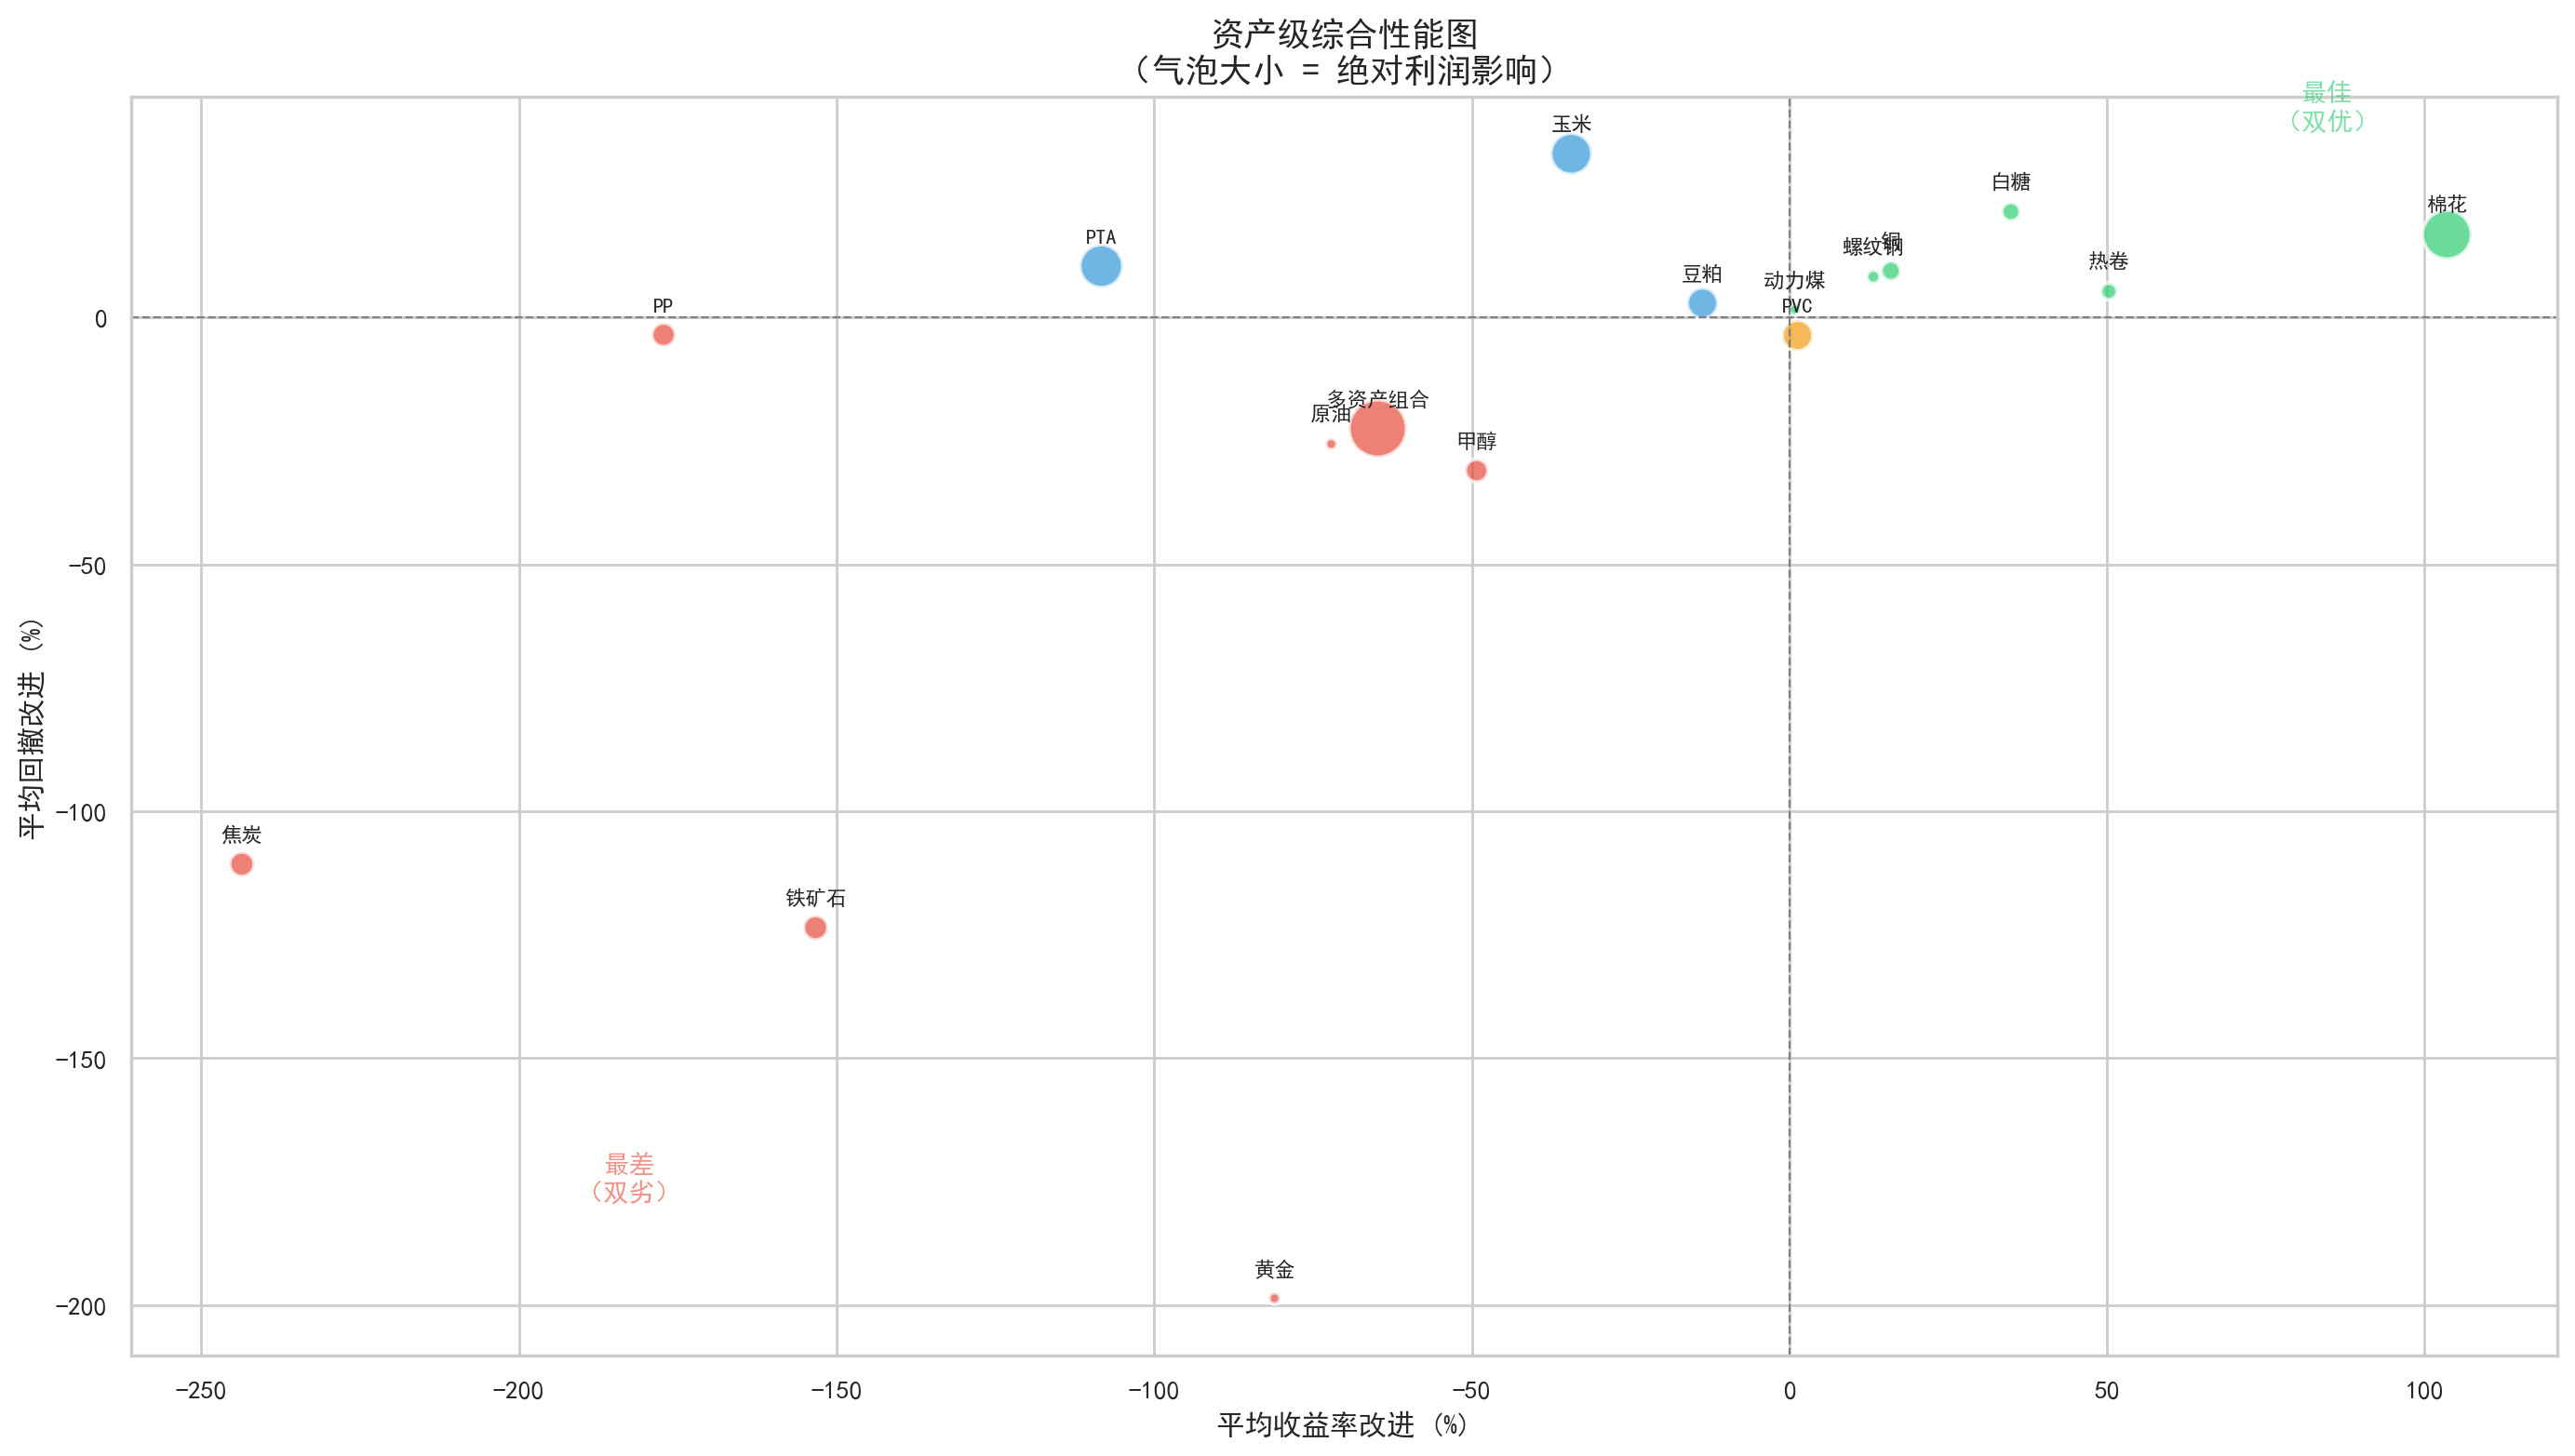
\includegraphics[width=0.8\textwidth]{figures/chap4/fig21_comprehensive_bubble_cn.png} 
%     \caption{各资产综合性能气泡图}
%     \label{fig:highdimcompbubble}
% \end{figure}

\begin{figure}[!htbp]
    \centering 
    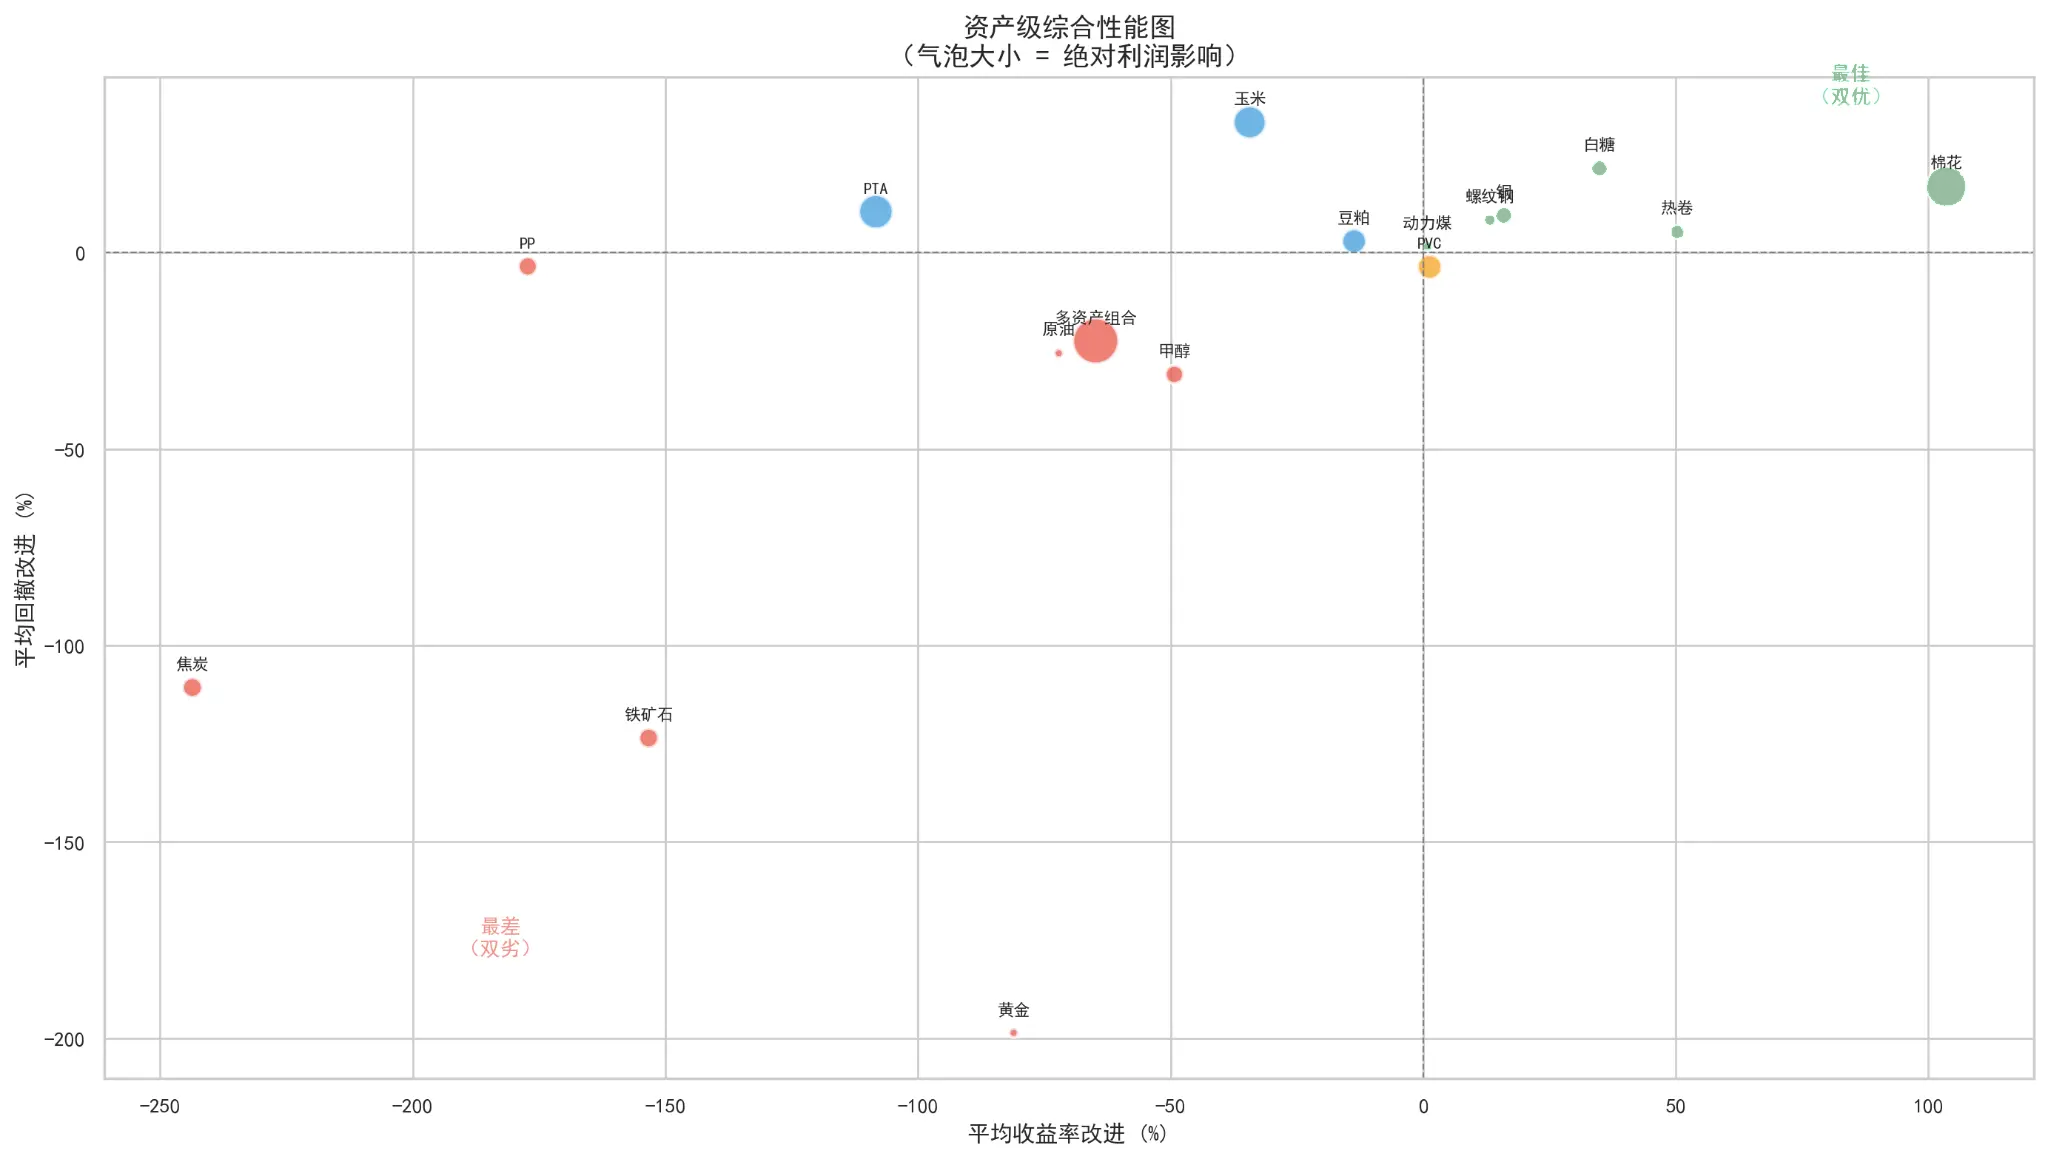
\includegraphics[width=0.8\textwidth]{figures/chap4/图3.23改.png} 
    \caption{各资产综合性能气泡图}
    \label{fig:highdimcompbubble}
\end{figure}

高收益但伴随较大回撤的策略在实际部署中可能因触及止损线或追加保证金而被迫平仓，难以稳定实现长期复利。因此，除收益率之外，本节进一步从风险控制角度分析赛马场竞争机制的表现。
图\ref{fig:highdimcomprehensivebubble}列出了赛马场竞争机制成功降低最大回撤的八个案例，覆盖投资、分类和回归三类任务。白糖投资任务中，基准模型最大回撤为57.08\%，赛马场竞争机制将其压缩至19.18\%，降幅66.4\%。

% \begin{figure}[h!]
%     \centering 
%     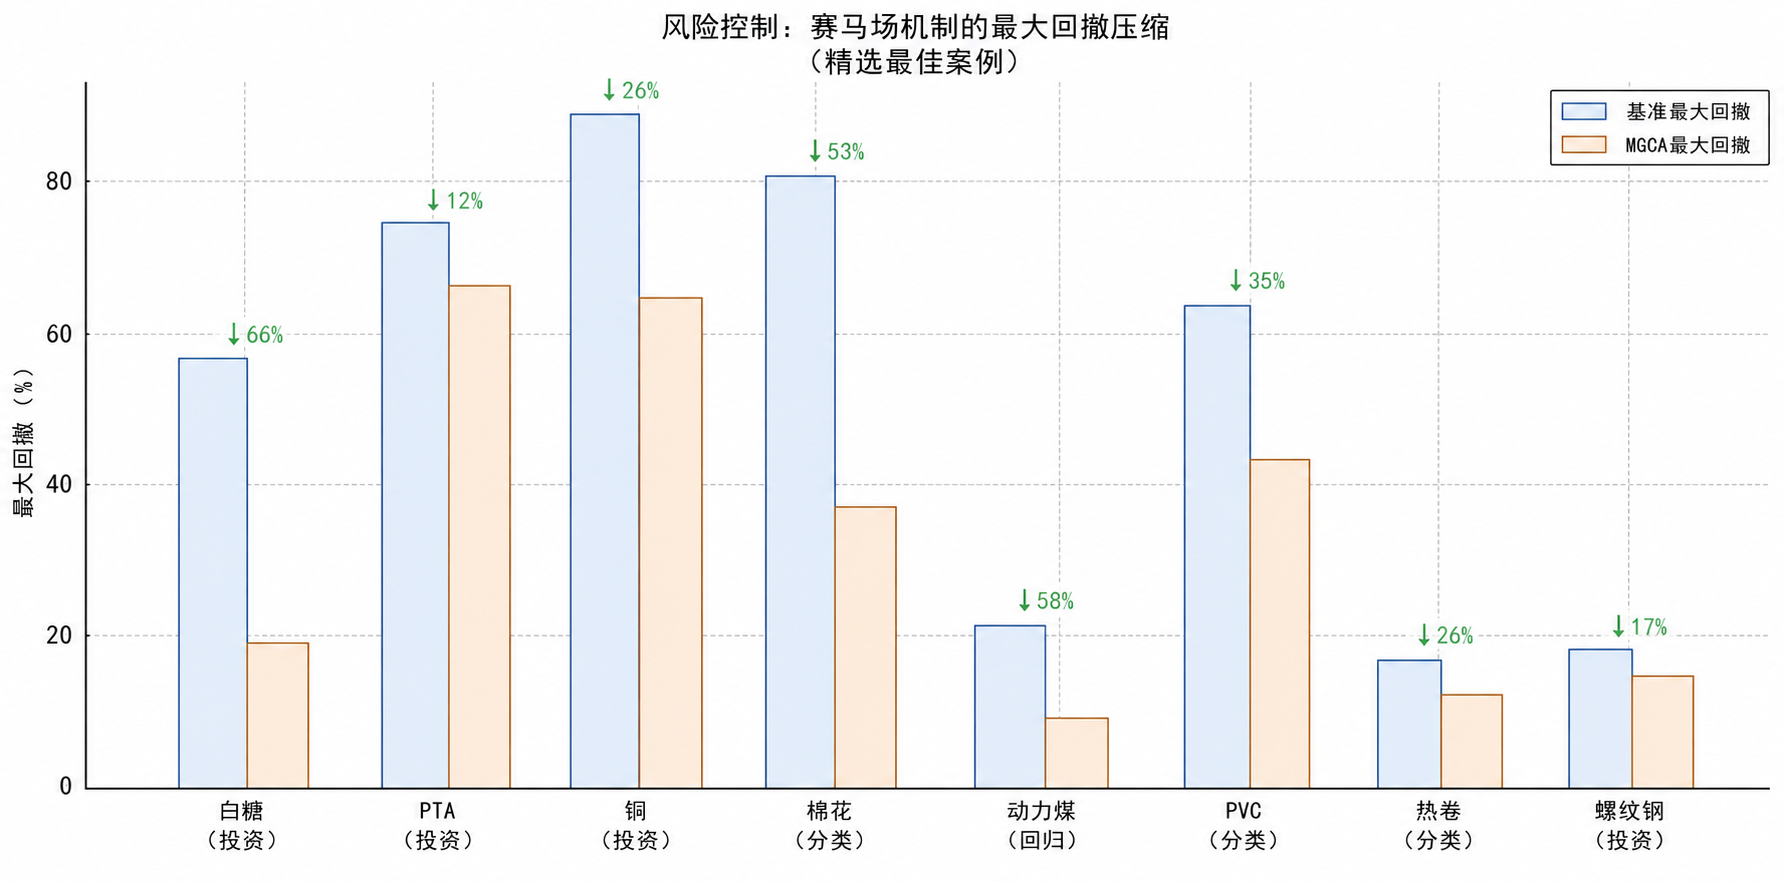
\includegraphics[width=0.8\textwidth]{figures/chap4/fig12_drawdown_comparison_cn.png} 
%     \caption{赛马场竞争机制的风险控制效果——最大回撤对比（精选最佳案例）}
%     \label{fig:highdimcomprehensivebubble}
% \end{figure}

\begin{figure}[!htbp]
    \centering 
    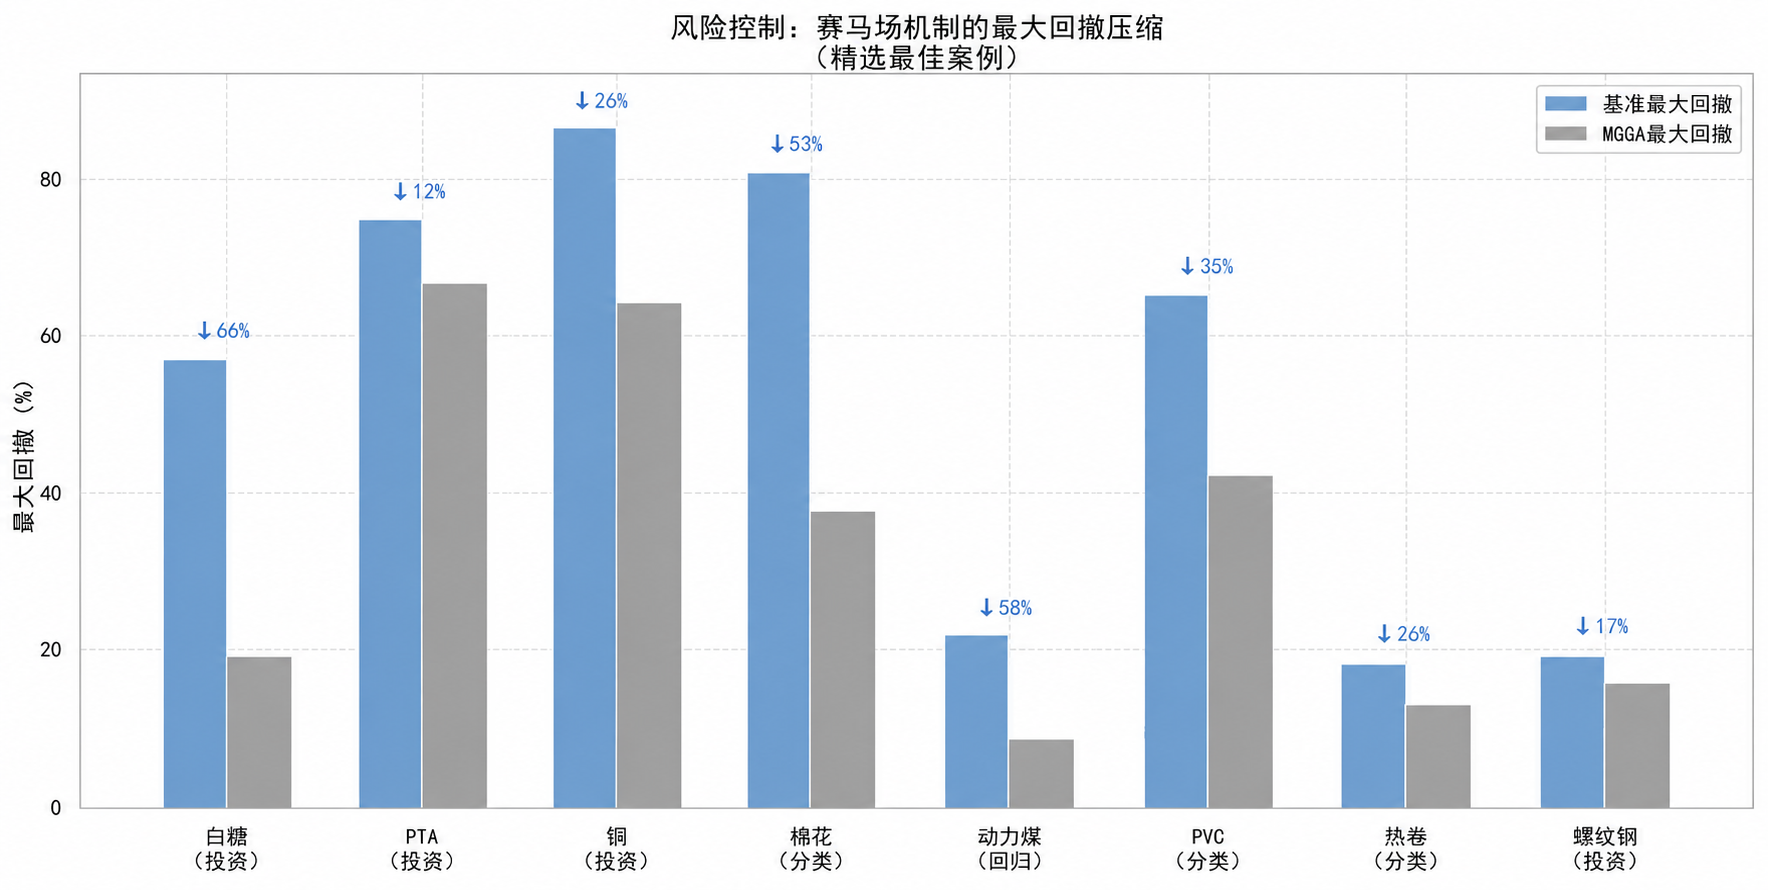
\includegraphics[width=0.8\textwidth]{figures/chap4/图3.24改.png} 
    \caption{赛马场竞争机制的风险控制效果——最大回撤对比（精选最佳案例）}
    \label{fig:highdimcomprehensivebubble}
\end{figure}

棉花分类任务中，基准模型最大回撤为80.94\%，赛马场竞争机制将其压缩至37.97\%（降幅53.1\%）。铜投资任务从86.93\%降至64.65\%（改善25.6\%），PVC分类任务从64.88\%降至42.42\%（改善34.6\%），动力煤回归任务从21.50\%降至8.96\%（改善58.3\%）。上述数据说明，回撤控制方面的改进在多个资产和任务中均有体现。

图\ref{fig:highdimriskreturnmigration}的风险-收益迁移散点图中，每个箭头代表一个资产从基准模型（灰色点）到赛马场竞争机制（红色点）的迁移轨迹，向左上方移动表示回撤降低同时收益提升。
赛马场竞争机制并非简单平均模型输出，而是根据市场环境动态调整模型权重，以兼顾多样性保持与风险控制。

% \begin{figure}[h!]
%     \centering 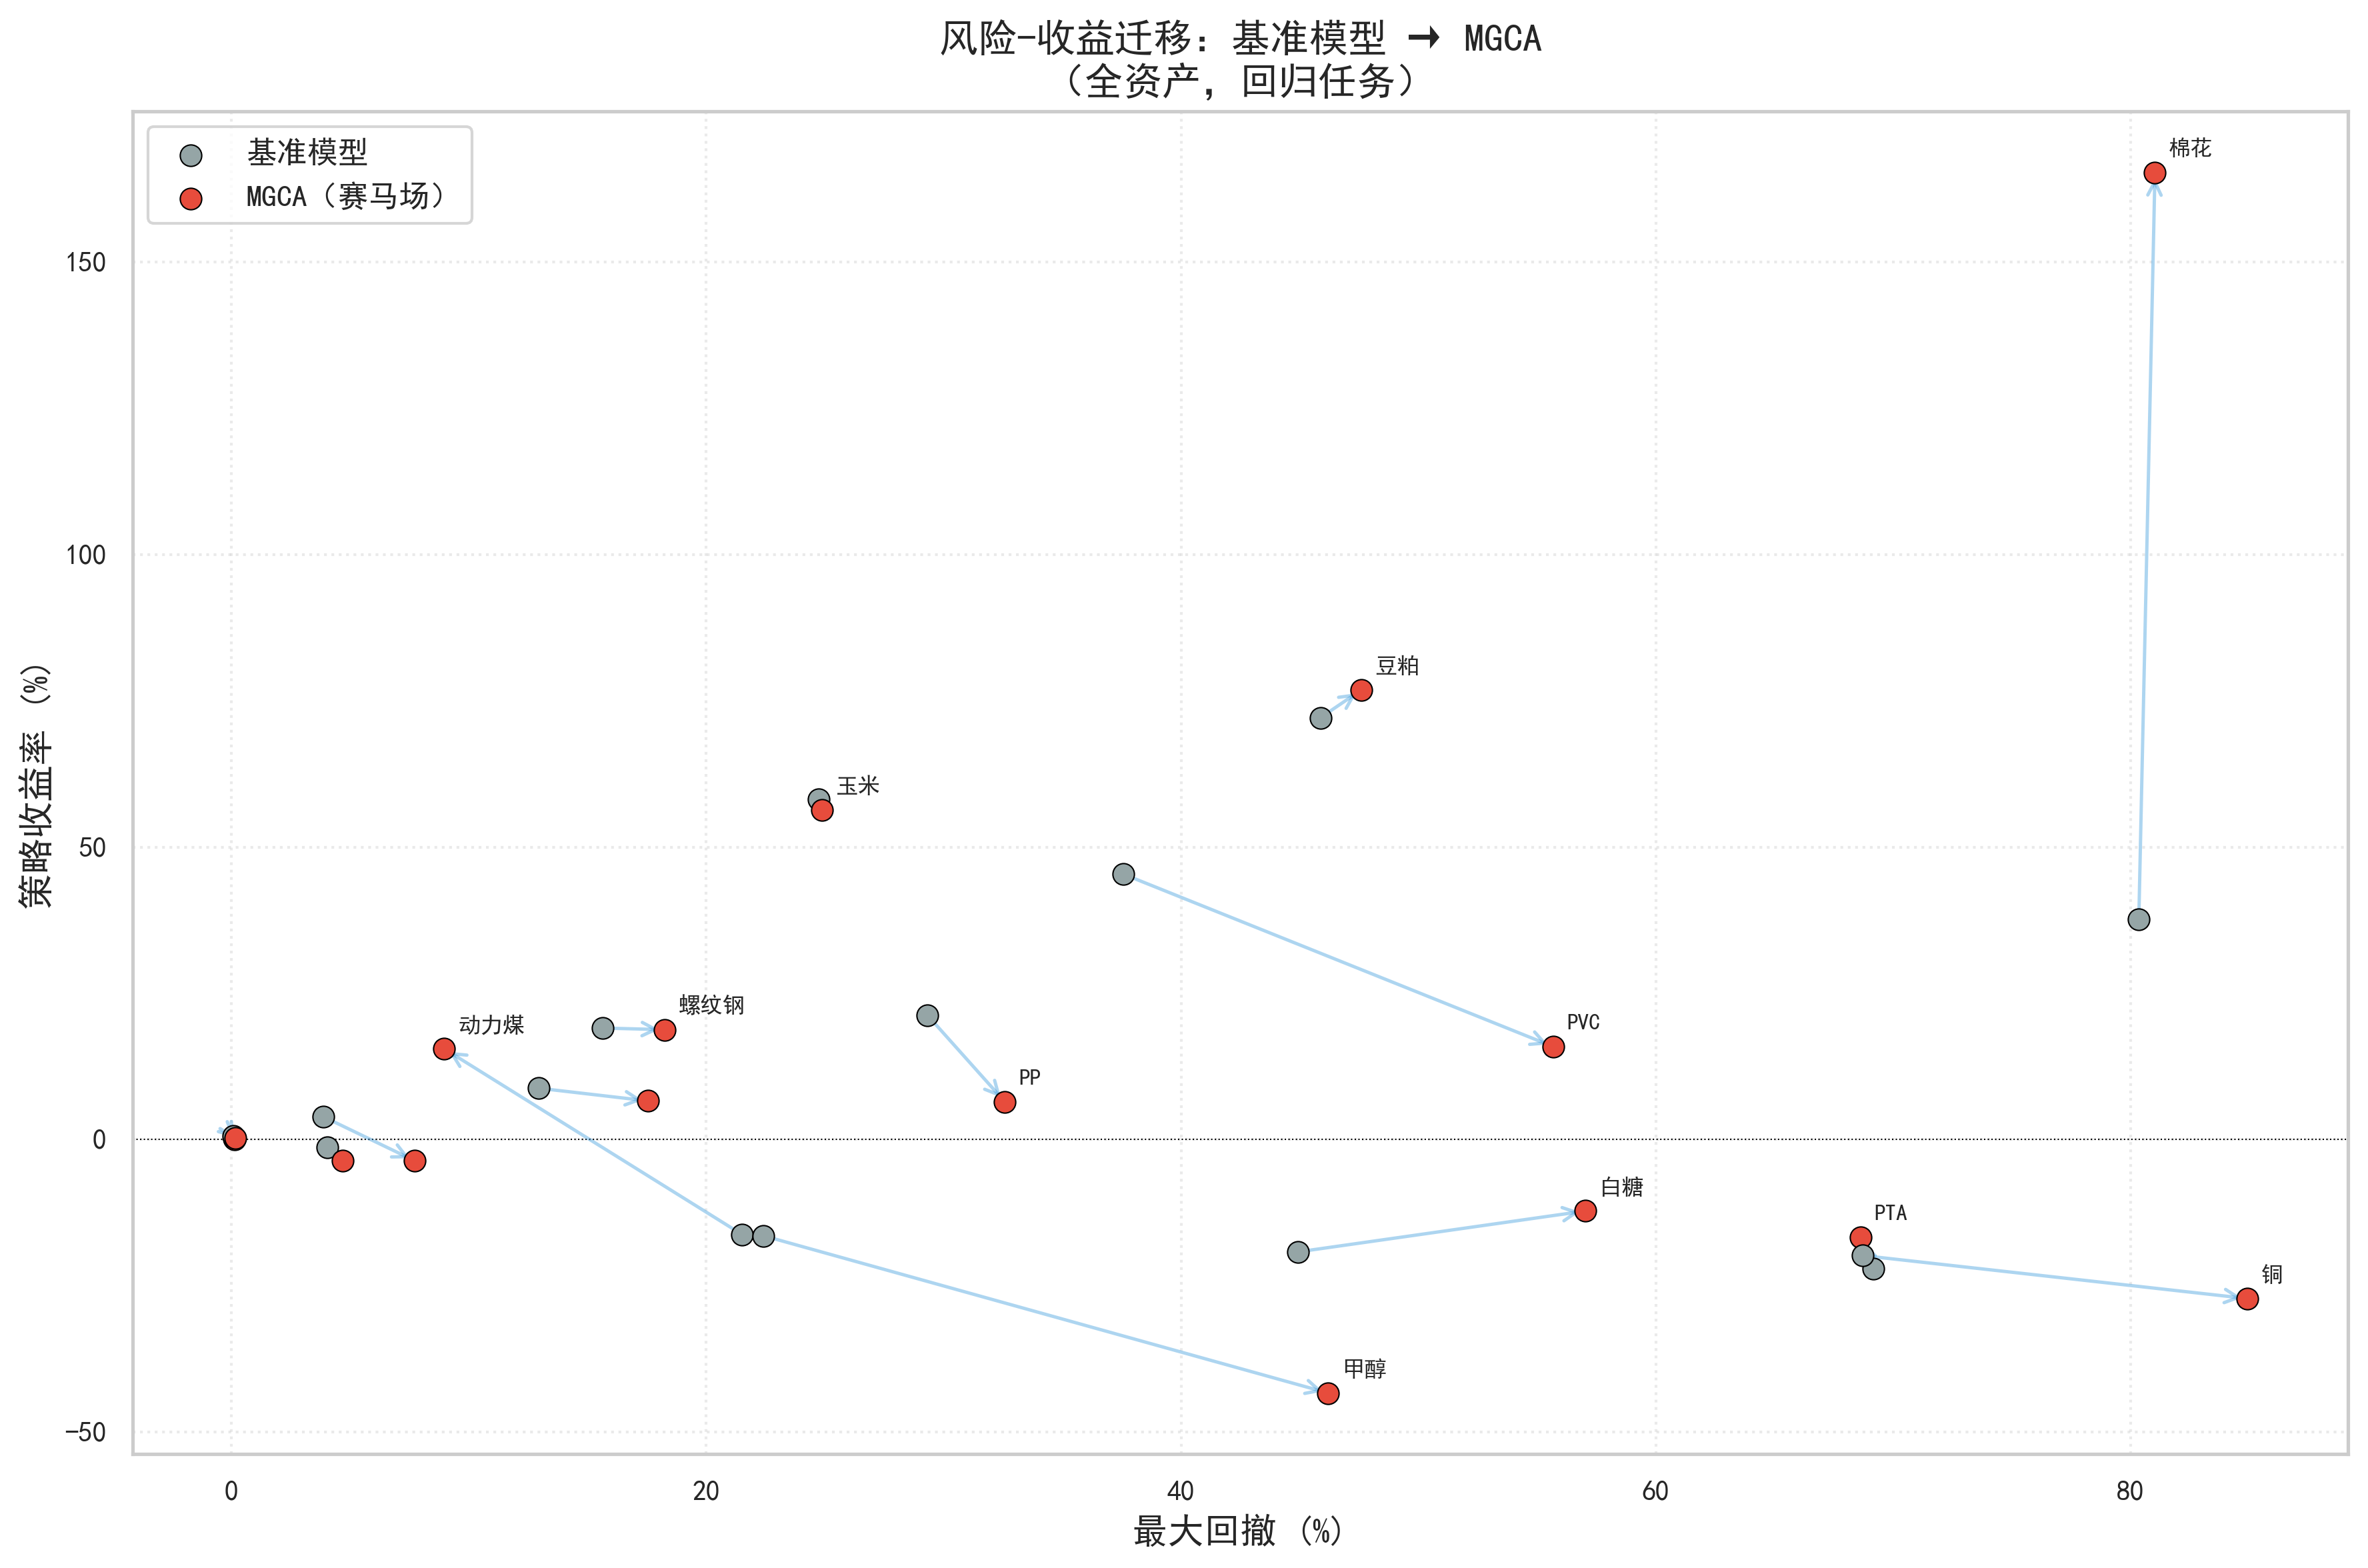
\includegraphics[width=0.8\textwidth]{figures/chap4/fig13_risk_return_migration_cn.png} 
%     \caption{风险-收益迁移散点图（赛马场竞争机制 vs. 基准模型）}
%     \label{fig:highdimriskreturnmigration}
% \end{figure}

\begin{figure}[!htbp]
    \centering 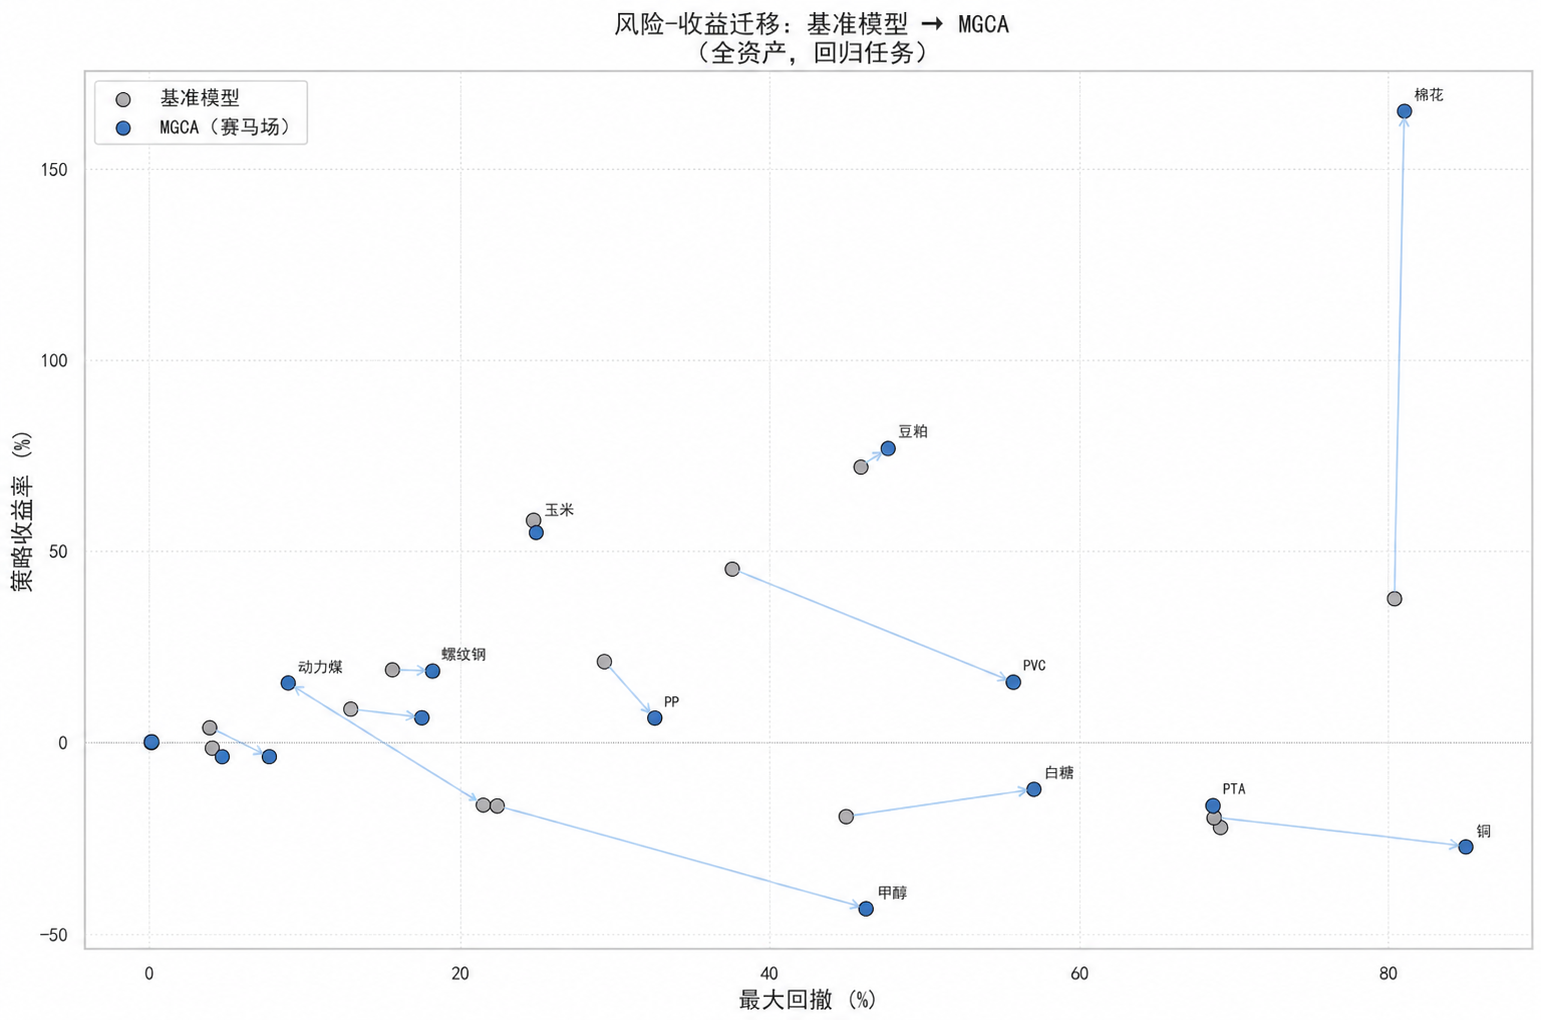
\includegraphics[width=0.8\textwidth]{figures/chap4/图3.25改.png} 
    \caption{风险-收益迁移散点图（赛马场竞争机制 vs. 基准模型）}
    \label{fig:highdimriskreturnmigration}
\end{figure}



\textbf{隐式正则化与过拟合抑制}：传统正则化方法（如一阶/二阶范数惩罚、随机失活）作用于参数空间或特征空间，赛马场竞争机制则在模型选择层面实施筛选——当某个生成器在训练集上表现尚可但验证集性能下降时，动态筛选机制会降低其权重乃至将其淘汰。这种基于泛化性能的动态筛选更直接地面向样本外表现，而不是只通过限制模型复杂度来降低过拟合风险。能源多资产组合和农业多资产组合的亏损转盈利案例（分别实现+202.85\%和+174.13\%的改进）与该解释方向一致：基准模型可能因过度拟合品种间的虚假相关性而亏损，赛马场竞争机制通过持续监控分布外表现，可能降低了对这类相关性的依赖。

\section{本章小结}
本章围绕对冲基金交易决策链条中的高维金融因子建模环节，讨论资产选择背后的因子表征依据形成问题。这里的因子表征依据并不是对交易结果进行事后解释，而是在第2章形成多资产配置入口的基础上，进一步识别哪些高维金融因子能够为资产选择提供稳定、可解释和可迁移的支撑信息。针对高维因子空间中的信息压缩、非对称竞争与过早收敛问题，本章引入了基于赛马场竞争机制的动态演化学习方法。

在方法设计上，本章首先通过多编码器表示学习缓解异构金融特征混合建模带来的结构丢失问题，随后利用赛马场竞争机制组织模型群体进行“评估—培养—淘汰—对齐”的循环演化。成熟—新生模型的双向知识迁移机制，将成熟模型的稳定表征与新生模型的差异化探索结合起来，形成“稳定继承—差异探索—反向校正”的优化过程，从而降低模型群体过快收敛到单一优势路径的风险。由此，本章方法以动态选优回应非对称竞争，以模型替换回应过早收敛，以双向知识迁移回应有效因子表征的持续修正需求。

在实验层面，超过60组对比实验表明，赛马场竞争机制在回撤控制方面的改进较收益率改进更为一致，模型分歧约束在风险暴露控制中的隐性作用也在多个任务类型中有所体现。相关结果说明，该机制并非单纯追求训练误差最小化，而是在模型多样性保持、动态筛选和风险暴露控制之间进行权衡。这种以模型群体交互、动态反馈和策略适应为核心的训练思路，也与多智能体强化学习中通过多主体交互提升复杂环境适应性的研究取向相一致\cite{lowe2017multi}。

本章接续第2章投资组合管理任务，从高维金融因子层面讨论支撑资产选择的表征依据。第2章关注多资产配置结果，本章关注支撑该配置结果的因子表达与动态竞争机制，二者在交易任务链条中形成前后承接。后续第4章将在因子建模基础上转向时序结构识别，讨论因子依据形成之后，如何判断市场结构和交易时机是否成立。

     \chapter{面向时序结构识别的逆向师生蒸馏学习方法}

\section{问题的提出}



\subsection{波浪结构识别的量化难点与高频噪声干扰}

前两章分别从投资组合管理和高维金融因子建模角度讨论了资产配置与因子依据问题，但在真实交易过程中，资产和因子依据并不能直接转化为交易时点。即便某一资产具备配置价值，仍需进一步判断当前市场结构是否支持进场，以及趋势、反转或震荡状态是否具有交易意义。因此，本章进入对冲基金交易决策链条中的时序结构识别环节，以波浪结构识别作为具体切入点，研究如何在高噪声、非平稳的金融时间序列中识别趋势结构、结构边界与有效波段。

艾略特波浪理论由艾略特于20世纪提出，其核心观点是市场波浪运动遵循``五浪推进+三浪调整''的循环模式，并在不同时间尺度上递归嵌套，呈现较明显的分形特征。相关研究曾将艾略特波浪思想用于股票市场结构分析与推荐场景，说明该理论在刻画趋势延续和反转结构方面具有一定应用基础\cite{tirea2012stock}。不过，本文并不把波浪理论理解为人工划线规则的简单复用，而是借用其层级嵌套和趋势—调整结构视角，将其转化为可监督、可检验的时序结构识别问题。图~\ref{fig:placeholder}展示了艾略特波浪理论的基本结构，包括五浪推进与三浪调整的典型形态及其分形嵌套关系。

\begin{figure}[htbp]
    \centering
    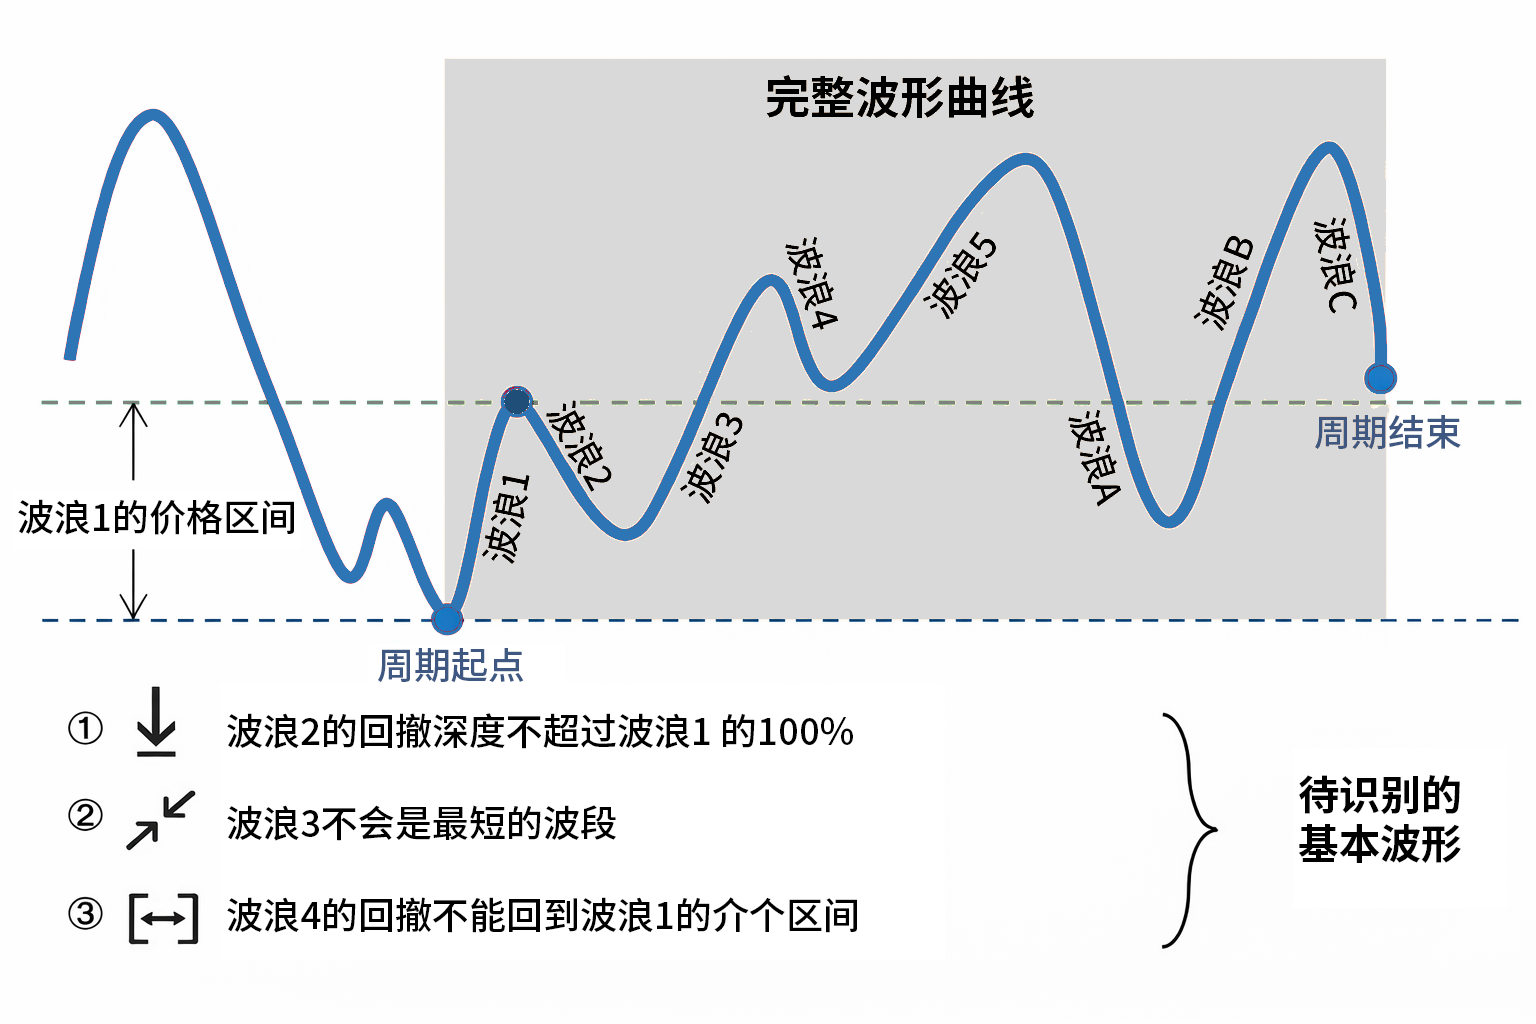
\includegraphics[width=1\linewidth]{figures/chap5/图4.1改.png}
    \caption{艾略特波浪理论}
    \label{fig:placeholder}
\end{figure}

在本章语境下，波浪结构被处理为金融时序结构的一种可操作化表达。交易时机判断不只取决于单一价格点位，还取决于价格路径是否已经形成相对稳定的趋势结构、转折结构或突破结构。然而，金融市场固有的高频噪声与结构模糊性会使部分局部波动被误识别为有效波段。高频交易与市场微观结构研究提示，噪声放大和短周期扰动会持续影响金融序列的可建模稳定性\cite{ba2019highfreq}。在这种环境下，传统依赖人工划分的波浪理论面临明显瓶颈：已有研究指出，波浪边界具有较强主观性，不同分析者之间的划分结果容易出现不一致\cite{wawer2024large}。

除人工划分差异外，波浪结构识别还受到市场状态变化本身的影响。经典区制转换模型表明，金融时间序列可能在不同市场状态之间切换，单一静态规则难以持续适配状态转移后的价格结构\cite{hamilton1989regime}。因此，波浪尺度会随着市场波动强度和状态转换过程动态变化，规则驱动方法即便在局部样本中有效，也难以长期保持稳定。

具体而言，波浪结构量化主要面临三类问题。第一，结构边界具有模糊性，同一段价格序列可能被划分为不同浪型；第二，波浪结构具有多尺度嵌套特征，需要同时识别推进浪、调整浪及其递归关系；第三，高频噪声会产生局部伪结构信号，使模型难以区分真实趋势转折与短暂价格扰动。因而，解决这一矛盾不能只停留在规则修补层面，还需要借助表示学习和结构校正机制对波浪边界进行更稳定的刻画。

数据驱动方法为金融时序建模提供了重要工具，但其有效性并不自动等同于波浪层级结构的稳定识别。金融深度学习研究说明，深度模型能够刻画复杂价格形成过程中的非线性关系\cite{sirignano2021universal}。但是，这类模型的主要目标通常是预测未来价格、收益方向或状态标签，而不是显式识别波浪边界、波段层级和结构转换位置。换言之，预测精度提高并不必然意味着模型已经理解了价格运动的层级结构。对于本章而言，关键问题不是继续证明深度模型能够进行价格预测，而是进一步说明如何把局部价格事件组织为结构清晰、边界可校正、具有交易含义的时序结构。

上述问题共同表明，金融时序结构识别不能被简化为一般价格预测或普通分类任务。金融资产收益序列普遍存在尖峰厚尾、波动聚集等经验特征，高频噪声与极端波动会进一步干扰局部结构识别\cite{Cont2001Empirical}。在这种数据环境下，模型即便在局部预测上有效，也未必能够形成稳定的层级结构表示。相关金融深度学习综述也表明，现有研究更多集中于直接价格预测或分类标签\cite{OZBAYOGLU2020106384}。因此，本章在一般深度预测模型之外，引入能够表达波浪结构、刻画局部事件边界并抑制高频伪结构干扰的标注与蒸馏机制，为后续四元分形事件识别和逆向师生蒸馏方法奠定问题基础。

\subsection{传统单向教师蒸馏范式在波浪结构识别中的局限性}

知识蒸馏由Hinton等人提出，主要通过教师模型向学生模型传递软标签或中间层表示，以改善模型泛化能力\cite{hinton2015distilling}。后续研究虽然将蒸馏方法扩展到多教师蒸馏、在线蒸馏和互学习等形式，但其基本逻辑仍多围绕教师模型向学生模型传递知识展开。不过，在波浪结构识别场景中，蒸馏机制面对的核心问题并不是学生模型能否模仿教师模型，而是教师模型的结构判断是否足够稳定、是否会把局部噪声误判为有效波段，并通过软标签传递给学生模型。

在时序结构识别任务中，蒸馏机制的作用不能仅理解为模型压缩。教师模型若对局部高频波动形成过度自信判断，学生模型会被迫继承这种偏差，最终导致结构边界识别不稳定。对于交易流程而言，这种偏差会表现为买入时机提前、滞后或误触发。因此，逆向师生蒸馏在提升模型泛化能力的同时，引入学生模型对复杂局部结构的反向校正，以降低单一强模型对伪趋势和噪声结构的误判。

多主体协同学习为这种反向校正提供了可借鉴的组织思路。多智能体系统强调多个学习主体之间的协作、竞争与信息共享，有助于在非平稳环境中形成更具适应性的策略\cite{lee2007multiagent}。但是，已有多主体方法并不能直接解决波浪结构识别中的边界模糊和类别不平衡问题。对本章而言，多主体协同的价值主要体现在允许不同模型对同一局部结构形成差异判断，并利用这种差异约束教师模型的过度自信输出，而不是简单增加模型数量。

进一步看，多智能体强化学习相关综述强调，多主体学习并不只依赖单个最优策略，而是通过多个学习主体在共享环境中的交互来提升复杂环境适应性\cite{du2019survey}。这一思路对本章的启发在于，波浪结构识别中的不同模型判断应当被用于相互校验，而不应让单一教师模型长期垄断结构边界定义。

同时，单向教师蒸馏还可能强化强模型主导下的结构偏差。生成对抗网络研究中的模式坍缩概念提示，在对抗或博弈式训练过程中，模型输出可能逐渐收缩到少数优势模式\cite{goodfellow2014generative}。在金融时序结构识别中，类似风险表现为：强模型在训练后期逐渐主导结构判断，使弱模型难以保留对少数类、极端波动或局部反转结构的探索能力，最终造成结构表达退化。常规``教师到学生''的单向机制在金融市场这种高度非平稳环境中，缺乏必要的自我纠错能力。

从信息传递角度看，传统蒸馏中的软标签虽然包含类间关系信息，但这种信息传递通常是单向且相对静态的。知识蒸馏综述也表明，蒸馏知识可以来自响应输出、中间特征和样本关系等不同层次\cite{gou2021knowledge}。这一点说明，蒸馏机制本身具有较强的扩展空间，但在市场剧烈波动期间，教师模型仍可能对某类波浪结构产生系统性偏差；学生模型如果过度拟合教师输出，就难以通过自身探索发现更准确的结构边界。因此，本章强调的逆向师生蒸馏并不是简单让弱模型反过来替代强模型，而是在结构识别误差出现时，将学生模型捕捉到的局部差异作为反向约束信号，用于修正教师模型对伪结构和边界位置的误判。

基于上述分析，本章需要解决的关键问题可以进一步凝练为三个层次：第一，如何将具有主观解释色彩的波浪形态转化为边界清晰、可重复标注的结构事件，使趋势结构识别具备可监督训练基础；第二，如何在强噪声和类别不平衡条件下抑制强模型对局部伪结构的过拟合，使结构边界识别不被单一高置信度判断锁定；第三，如何判断已识别的结构信号是否能够延续为具有交易意义的有效波段，从而真正服务于交易流程中的交易时机判断。因此，本章并不把目标设定为单纯提高价格方向预测精度，而是围绕``结构可量化、边界可校正、信号可交易''构建时序结构识别方法。后续方法设计中，四元分形事件主要回应结构量化问题，逆向师生蒸馏主要回应边界校正与噪声抑制问题，带鱼短鱼机制则用于补充趋势有效性判别。



\section{相关工作}

围绕金融时序结构识别，已有研究大体可以分为三类：一是以波浪理论和技术形态分析为代表的结构解释方法，二是以深度序列模型、注意力机制和生成式建模为代表的数据驱动识别方法，三是以知识蒸馏和多模型协同为代表的泛化提升与误差校正方法。这些研究分别从市场形态、序列表示和模型迁移角度提供了有益基础，但与本文关注的交易时机识别任务相比，仍存在结构边界不清、局部噪声干扰、预测输出难以回到波浪层级以及单向知识传递容易放大教师偏差等问题。因此，本节并不把相关工作简单归纳为价格预测或模型分类问题，而是围绕“结构能否被清晰标注、边界能否被稳定校正、识别结果是否具有交易延续性”三个方面展开讨论。

传统波浪理论强调价格运动中趋势推进与调整回撤的层级关系，为观察金融序列的结构性变化提供了直观框架。相关实证研究也尝试检验艾略特波浪理论在金融市场预测中的有效性\cite{dangelo2017effectiveness}。这说明波浪理论具有一定的市场解释价值，但其应用过程往往依赖人工识别和经验划分。对于可重复训练的深度学习框架而言，真正困难的并不是确认市场中存在某种形态经验，而是将波浪起止点、层级嵌套关系和有效波段边界转化为可监督、可回溯且可在不同样本中重复执行的结构事件标签。

深度时序模型为金融序列中的趋势识别和状态判别提供了新的工具。股票价格预测研究表明，循环神经网络类模型能够从高噪声价格序列中提取局部时序模式\cite{nelson2017stock}。这类研究为金融序列建模提供了数据驱动基础，但其目标通常是价格拟合或方向预测，模型输出并不会自动对应波浪边界。对于本章任务而言，预测曲线是否贴近真实价格只是一个中间问题，更关键的是模型能否判断局部转折是否构成有效结构、识别出的结构能否延续为具有交易意义的波段。

近年来，长短期记忆网络仍被用于刻画金融趋势变化中的时间依赖关系\cite{xie2025lstm_trend}。这一方向说明门控循环结构在处理局部趋势变化时仍有价值，但单一序列模型容易把短期波动误认为趋势变化，也可能忽略波浪结构中的层级关系。进一步的混合时序模型研究则表明，将循环结构与其他深度模块结合，可以增强模型对复杂金融序列的表达能力\cite{ma2025transformer_lstm}。不过，表达能力增强并不必然意味着结构识别能力增强；如果缺少结构化标签和边界校正机制，模型仍可能在高频噪声、局部反转和短周期震荡中学习到伪结构。

在结构识别相关任务中，已有研究开始将深度序列模型用于股票状态类别识别\cite{wang2025lstm_classification}。状态分类把连续价格序列转化为离散市场状态，有助于缩小预测任务与交易判断之间的距离。与此同时，注意力机制与长短期记忆网络结合的研究表明，模型可以通过关注关键时段特征来改善金融序列状态判别\cite{li2024attention_lstm}。这类研究进一步说明，数据驱动模型已经能够从金融序列中提取部分趋势、状态和局部变化信息；但波浪结构识别不仅要求模型判断“处于何种状态”，还要求模型回答结构边界在哪里、局部反转能否延续、信号是否能够转化为可交易波段等问题。

生成式金融序列建模从另一侧拓展了时序结构研究。近期金融时间序列生成研究表明，生成式模型可以用于补充样本分布和模拟复杂市场状态\cite{vuletic2024fin}。这类工作对于缓解金融样本有限、市场状态覆盖不足等问题具有启发意义，但生成或补充数据本身不能直接解决波浪边界识别问题。若缺少结构化标签、边界校正和趋势有效性判别，生成模型仍可能在局部波动中放大伪结构，甚至把统计上相似但交易含义不同的片段混为一类。

国内相关研究也将生成对抗网络用于金融数据生成任务，为复杂金融序列分布建模提供了参考\cite{cui20241gan}。此外，深度生成模型被引入因子投资建模场景，说明生成式方法在金融表征学习中具有一定拓展空间\cite{ma2022deep}。这些研究共同说明，生成式方法能够服务于金融数据分布表达和样本扩展，但其作用仍主要体现在表征和数据层面。对于本文的波浪结构识别任务而言，仍需要进一步回答结构标签如何构建、类别不平衡如何处理，以及局部结构是否具有后续交易延续性等问题。

知识蒸馏和多模型协同方法为模型压缩、泛化提升和知识迁移提供了重要路径。相关知识蒸馏研究表明，蒸馏方法已经从单一教师—学生压缩范式扩展为多种知识迁移与模型协同形式\cite{huang2022distillation}。这一方向为本文引入逆向师生蒸馏提供了方法背景，但传统蒸馏更多强调强模型向弱模型传递知识，并未充分讨论学生模型对教师模型结构判断的反向校正作用。对于金融时序结构识别而言，强模型可能在局部噪声中形成过度自信的结构判断，若学生模型只能被动模仿，就可能继承这种偏差。因此，本章关注的不是一般意义上的模型压缩，而是利用模型间差异对强模型的结构边界判断进行反向约束。

基于上述不足，后文以波浪结构作为时序结构识别的具体场景，在四元分形事件标注方法的基础上，引入逆向师生蒸馏机制以提升结构识别的稳定性。与传统``强教师指导弱学生''的单向蒸馏不同，该机制强调当学生智能体在特定复杂结构上实现阶段性超越时，教师模型也应参考学生模型捕获的新分布特征，从而缓解强模型对局部高频噪声的过拟合问题。由此，相关工作所暴露出的主观标签、噪声干扰和单向蒸馏局限，构成了本章后续算法设计的直接动因。下一节将围绕结构标签构建、逆向师生蒸馏和趋势有效性判别三个层面展开方法设计。

\section{逆向师生蒸馏方法}

本节介绍面向时序结构识别的逆向师生蒸馏方法，并按照前文提出的三个问题展开。首先，针对波浪结构主观性强、边界不清的问题，通过四元分形事件将价格序列中的转折、交叉和突破结构转化为可监督标签；其次，针对强模型容易被局部噪声误导的问题，通过逆向师生蒸馏机制在多模型之间传递误差信息与结构边界信息，抑制强模型对局部伪结构的过拟合；最后，针对结构信号是否真正具有交易意义的问题，通过带鱼短鱼机制判断已识别结构能否延续为有效趋势。上述设计共同服务于交易流程中的交易时机判断，使结构信号从形态描述进一步转化为交易时机判断依据。

为避免将本章方法理解为单一分类模型，本节先从整体组织架构和任务设置两个层面说明方法设计。图\ref{fig:S2T-arch}展示了本章方法的三层组织结构：第一层将波浪结构转化为四元分形事件标签，第二层通过生成器组和判别器组构成逆向师生蒸馏系统，第三层将结构识别结果映射到分类与交易应用。图\ref{fig:S2T-task}进一步说明四元分形事件在多任务预测中的组织方式，为后续4.3.1的标签定义、4.3.2的模型构建和4.3.3的逆向蒸馏机制提供任务入口。

\begin{figure}[!htbp]
    \centering
    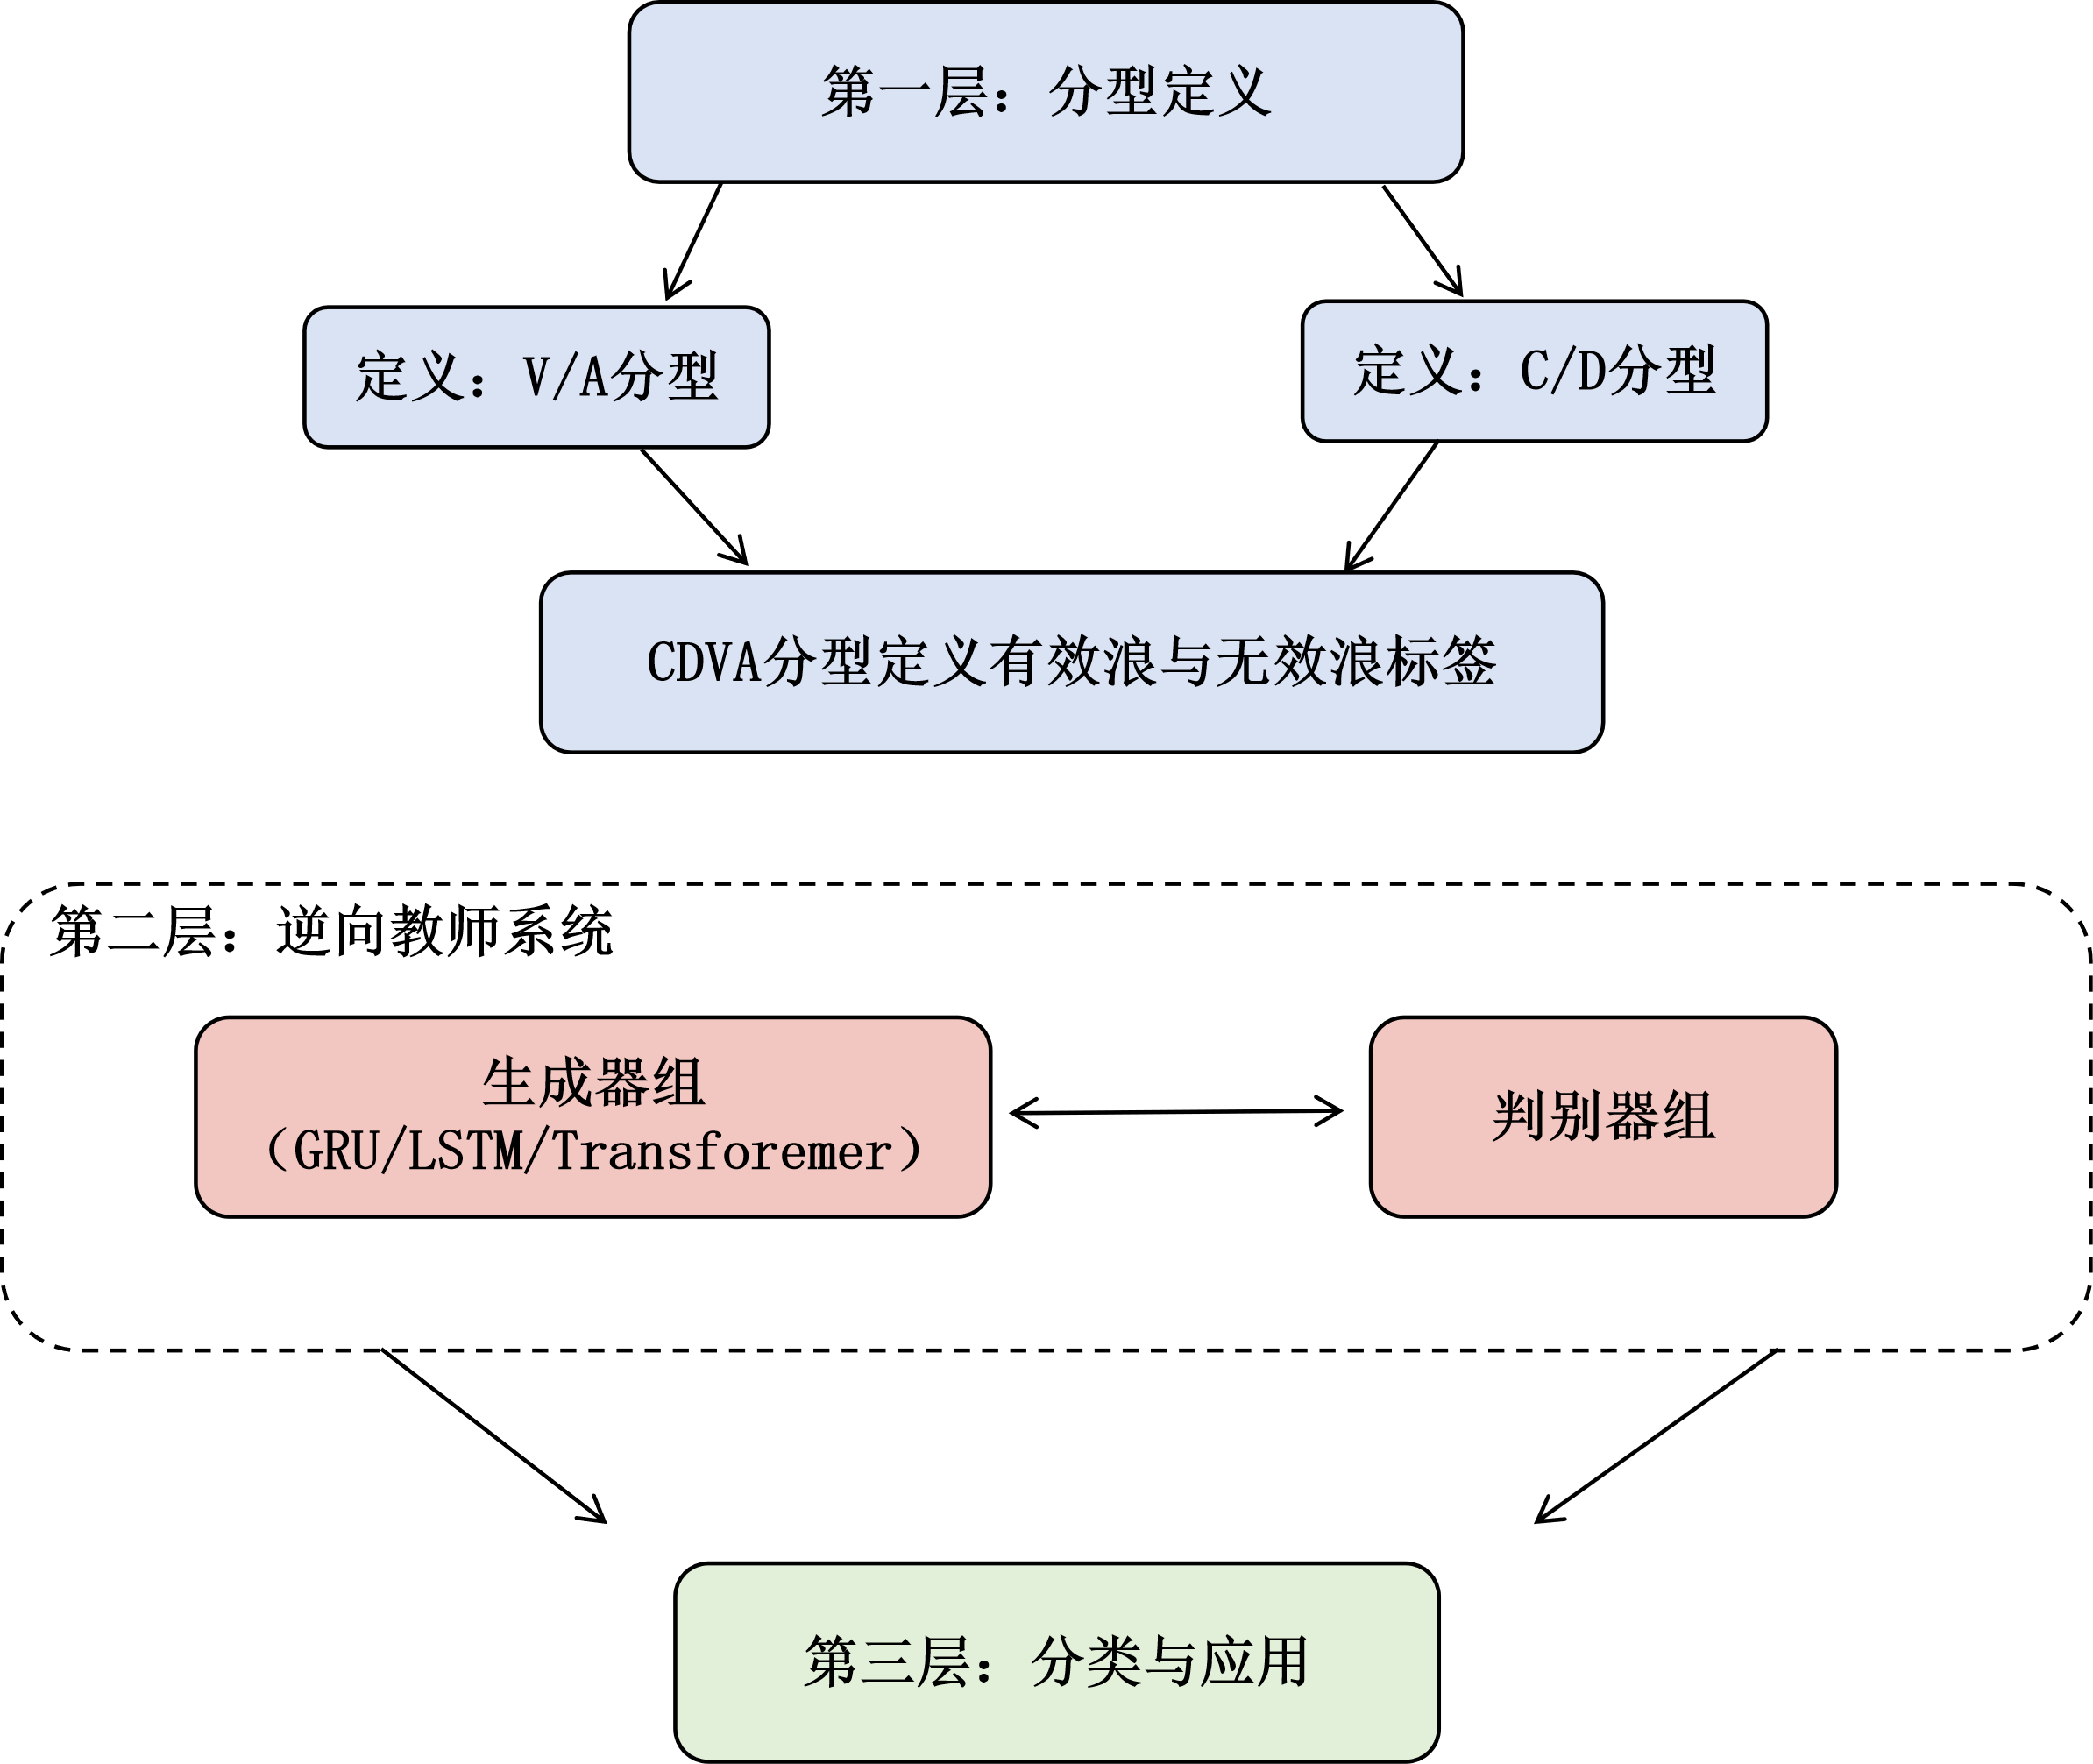
\includegraphics[width=0.8\textwidth]{figures/chap5/波浪架构.png}
    \caption{基于逆向师生蒸馏机制的时序结构识别组织架构}
    \label{fig:S2T-arch}
\end{figure}

\begin{figure}[!htbp]
    \centering
    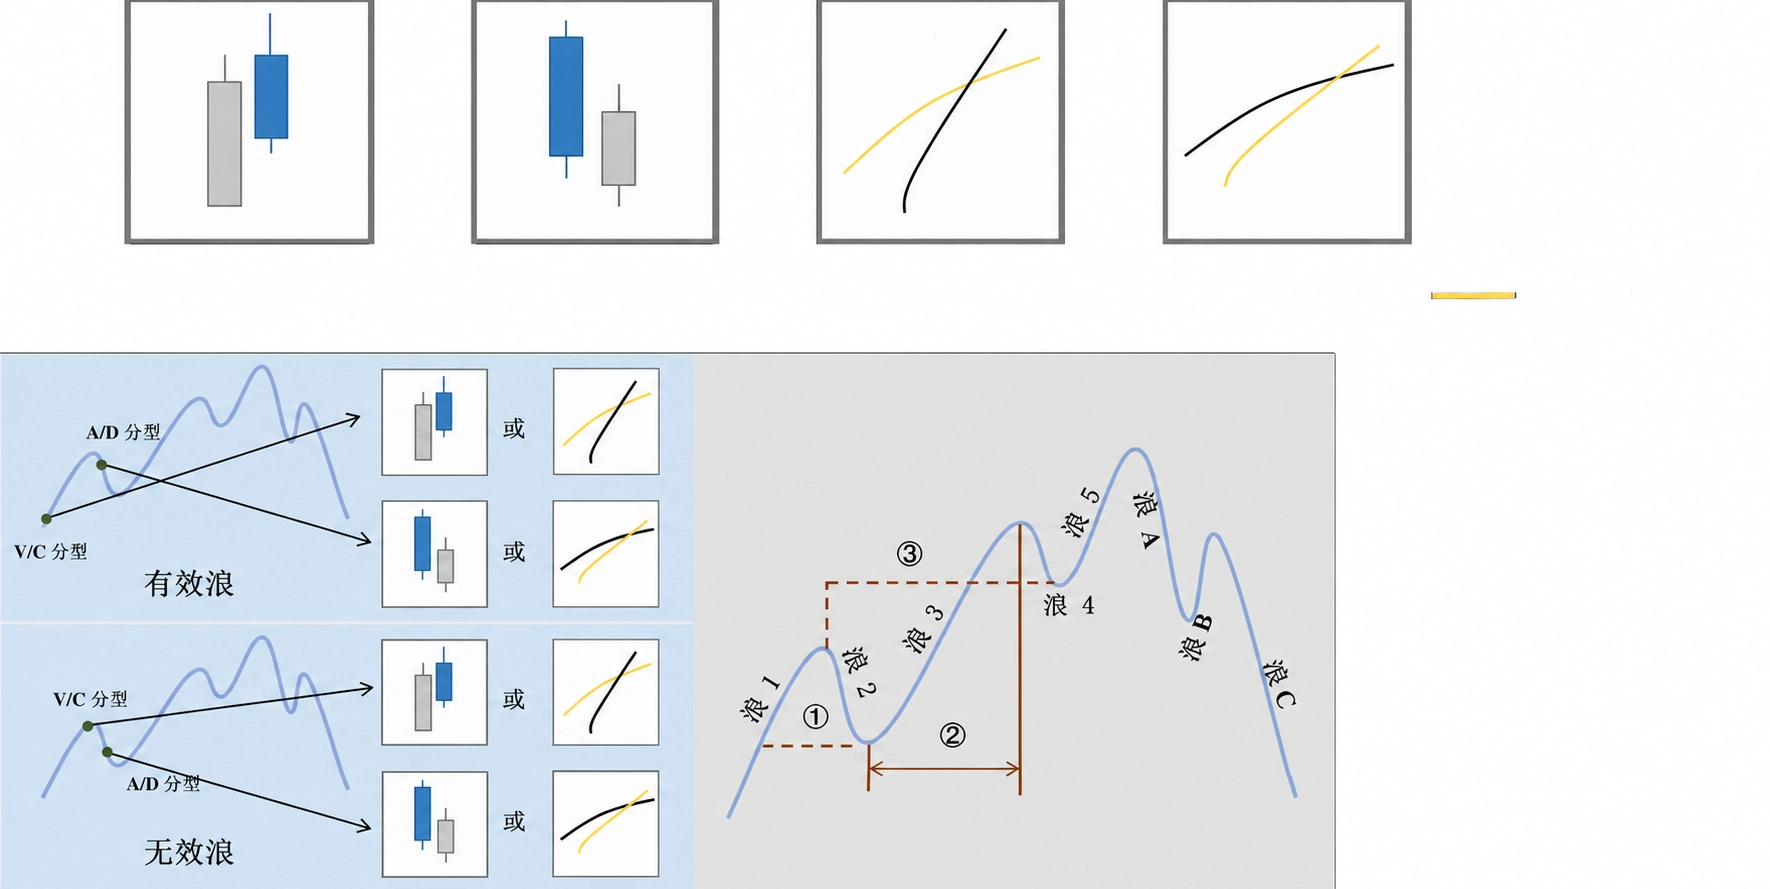
\includegraphics[width=0.8\textwidth]{figures/chap5/图4.3改.png}
    \caption{基于逆向师生蒸馏机制的时序结构识别任务}
    \label{fig:S2T-task}
\end{figure}

\clearpage

\subsection{四元分形事件标注方法与波浪结构量化重构}

``裸K线交易法''强调在交易图表中剔除均线、指数平滑异同移动平均线、布林带等衍生指标，仅依据原始K线（蜡烛图）的形态、组合排列及关键支撑阻力位分析市场微观结构。这类方法直观、贴近交易实践，但其判断过程很大程度上依赖视觉经验，长期缺乏可重复的数学边界。与之相对，传统深度学习模型虽然能够处理连续价格序列，却往往把价格变化压缩为浮点数张量，弱化了K线之间最基本的拓扑排列关系，使结构判定与模型输出之间缺乏直接对应。

基于这一问题，本章提出四元分形事件标注方法。其中，V（向上突破）与 A（向下跌破）分型对应于相邻K线之间最基础的突破与跌破结构。此类将交易经验规则转化为可计算结构标签的思路，与国内关于金融数据生成建模和结构化表示学习的研究取向具有一致性\cite{xu2024gan}。通过对前一周期实体边界与当前收盘价之间的关系进行明确刻画，原本依赖经验识别的K线排列被转化为可重复的二元事件标签。这样处理的目的，不是简单增加一组技术指标，而是为后续模型训练提供结构化输入，并使输出结果能够回到原始K线图上进行解释。换言之，四元分形事件标注方法试图在裸K线经验与深度模型之间建立可计算的对应关系，使模型识别结果具有较清楚的图形解释基础。

四元分形事件在本章中的作用，是将原本主观的波浪划分转化为可重复的时序结构标签。C/D事件刻画动量结构的方向切换，V/A事件刻画价格实体的局部突破与跌破，它们共同提供了趋势启动、趋势反转和结构确认的候选时点。因此，该标签体系不仅用于形态分类，也为交易时机判断提供可监督的结构化输入。

为了构建可用于深度模型训练的结构化波浪标签体系，本章基于动量类指标与K线结构行为，设计了四元分形事件：C（上穿）、D（下穿）、V（向上突破）、A（向下跌破）。相比传统波浪结构定义，该体系更易量化，边界也更便于在大规模时序数据上重复标注。四元分形事件的设计遵循两个原则：其一，C与D基于动量指标的方向切换，捕捉趋势的宏观转折信号；其二，V与A基于K线实体的价格突破，捕捉微观层面的结构性波动。这种宏观与微观相结合的标签设计，使得模型能够在多个时间尺度上同时学习波浪结构特征。

在构建C（上穿）与D（下穿）两类方向性切换分形时，本章引入了指数平滑异同移动平均线。指数平滑异同移动平均线由快速与慢速两条指数加权移动平均线构成，二者之差定义为动量线：

\begin{equation}
\mathrm{DIF}_t = \operatorname{EMA}_{\text{fast}}(P_t) - \operatorname{EMA}_{\text{slow}}(P_t),
\end{equation}

其中$P_t$为时刻t的收盘价。动量线的指数移动平均为信号线，二者之差称为柱状线：

\begin{equation} \mathrm{DEA}_t = \operatorname{EMA}_{\text{signal}}(\mathrm{DIF}_t) \label{eq:dea} \end{equation}

\begin{equation} \mathrm{MACD}_t = 2 \times (\mathrm{DIF}_t - \mathrm{DEA}_t) \label{eq:macd} \end{equation}

本章将指数平滑异同移动平均线重新解释为``分形结构触发器''：当动量线由下向上穿越信号线时记为C（金叉）；当动量线由上向下穿越信号线时记为D（死叉）。相比传统手工波浪划分，这种基于指数平滑异同移动平均线的结构事件更具可量化性、鲁棒性与可重复性。需要指出的是，指数平滑异同移动平均线本身作为滞后指标，其信号触发时间通常晚于价格的实际转折点，这一特性在后续的``带鱼短鱼''机制中将被进一步讨论与补偿。

在方向性切换分形的基础上，本章进一步定义基于K线实体突破的结构性波动事件（V/A）。给定上一周期实体上沿与下沿：

\begin{equation}
U_{t-1} = \max(\mathrm{open}_{t-1},\, \mathrm{close}_{t-1}),
\qquad
L_{t-1} = \min(\mathrm{open}_{t-1},\, \mathrm{close}_{t-1}),
\end{equation}

则当前周期的V/A信号定义为：

\begin{equation}
V_t = \mathbb{I}(\mathrm{close}_t > U_{t-1}),
\qquad
A_t = \mathbb{I}(\mathrm{close}_t < L_{t-1}).
\end{equation}

V描述价格向上穿越前实体上沿的``结构性突破''，常对应趋势波段的延续；A描述价格向下跌破前实体下沿的``结构性回落''，常预示反转或加速回撤。V/A的定义基于严格的价格边界，对噪声不敏感，可在高频/日频数据上稳定复现。与C/D分形相比，V/A分形具有更高的时间分辨率，能够在趋势内部捕捉到更细粒度的结构变化，为模型提供了互补的多尺度结构信息。

基于上述定义，四元分形标签体系将波浪结构识别转化为可重复的监督信号，并为后续 4.3 节的模型构建与 4.4 节的实验比较提供统一的结构标签基础。更重要的是，该标签体系使时序结构识别能够与交易时机判断建立直接联系：结构事件的出现对应潜在买卖时点，结构事件的持续与反转则决定该时点是否具备进一步交易价值。由此，四元分形事件在本章中不是附加的技术指标集合，而是把传统波浪形态转化为可学习结构输入的关键环节，直接回应了 4.1 节提出的结构量化问题。

\subsection{逆向师生蒸馏的误差信息传递与反向校正}

本节在四元分形事件标注方法的基础上，也说明逆向师生蒸馏机制如何服务于时序结构识别。与一般分类模型只关注标签预测不同，本节关注的是在高噪声、非平稳金融序列中，如何通过模型间误差信息传递抑制局部伪结构，使强模型在追求低损失的同时仍受到组内结构分布约束。由此，逆向师生蒸馏在本章中主要承担结构边界识别、噪声过滤与交易时机确认中的训练约束作用，而不只是模型压缩工具。

\noindent\textbf{状态空间构建与特征提取优化}\par

在明确了C、D、V、A四元分形事件的边界与触发条件后，本章将波浪结构识别转化为一个基于多变量时间序列的多任务学习问题。给定长度为T的金融时间序列$X = \{x_1, x_2, \dots, x_T\}$，其中$x_t \in \mathbb{R}^d$表示t时刻的d维特征向量，时间窗口大小为W，模型在t时刻的输入为$X_{t-W+1:t} \in \mathbb{R}^{W \times d}$。本章的任务目标是学习一个深度映射函数$f_\theta$，预测目标空间包含两部分：结构分类标签$y_t$ = ($y^C_t, y^D_t, y^V_t, y^A_t$)属于$\{0, 1\}^4$，其中$y^k_t = 1$表示第k类分形事件发生；结构持续时间$l_t$ = ($l^C_t, l^D_t, l^V_t, l^A_t$)$\in \mathbb{R}^4$，表示对应分形结构从触发到结束的时间跨度。整体任务形式化为：

\begin{equation}
    (\hat{\mathbf{y}}_t, \hat{\mathbf{l}}_t) = f_\theta(\mathbf{X}_{t-W+1:t})
\end{equation}

其中$\hat{y}_t \in [0, 1]^4$为各分形事件发生的预测概率，$\hat{l}_t$为预测的持续时间。通过这一形式化定义，传统波浪理论中主观、模糊的``形态识别''过程被严格转化为可端到端优化的多标签分类与回归联合预测任务。

在时序结构识别任务中，误差信息不仅表示分类错误，也反映模型对结构边界、趋势转折和局部噪声的判断偏差。逆向师生蒸馏的意义在于，当弱模型在某些局部结构上保留了更丰富的边界信息时，强模型可以通过反向校正避免过度收敛到单一高置信度判断，从而提升对复杂时序结构的识别稳定性。该机制对应 4.1 节提出的第二类问题，即传统单向蒸馏容易把强模型偏差传递给弱模型，导致交易时机判断提前、滞后或误触发。

\noindent\textbf{逆向师生蒸馏机制的核心逻辑与误差信息传递}\par

本章构建了由多生成器（预测网络）与多判别器（结构校验网络）组成的训练框架。生成器组由门控循环单元、长短期记忆网络与自注意力序列模型三类异质网络构成，以实现``局部短期记忆-全局长程依赖''的特征互补。自注意力序列模型生成器采用4层编码器结构，多头注意力机制的头数设为8，隐藏层维度为256；门控循环单元与长短期记忆网络生成器均采用双层堆叠结构，隐藏层维度设为128。判别器组由多层感知机与对应时序网络构成。模型输入包括开盘价、最高价、最低价和收盘价基础价格序列，并辅以多尺度趋势敏感指标（5日指数加权移动平均线、120日指数加权移动平均线）以及指数平滑异同移动平均线，同时包含各特征的一阶变化率，使生成器能够在``绝对水平-相对变化''两个维度中捕捉波段的结构转折行为。

选择门控循环单元、长短期记忆网络与自注意力序列模型三种异质架构作为生成器组的设计考量在于：门控循环单元具有较少的参数量和更快的收敛速度，适合捕捉短期局部模式；长短期记忆网络通过门控机制能够有效保留长期依赖信息，对中等时间跨度的结构特征具有优势；自注意力序列模型基于自注意力机制，能够在全局范围内建模任意位置之间的依赖关系，尤其擅长捕捉长程结构模式。三种架构的异质性确保了生成器组在特征空间中的探索多样性，为后续的蒸馏机制提供了差异化的知识来源。

为缓解模式崩溃问题，本章引入逆向师生蒸馏机制，并在训练中构建正向蒸馏与反向蒸馏的互补关系：正向蒸馏用于引导群体向当前较优解靠拢；反向蒸馏用于约束强模型过度依赖单一路径，使其参考弱模型保留的局部结构信息，从而降低模型群体同质化风险。

对于任意输入序列X，生成器G的输出包含四个结构分类任务（C/D/V/A）的logits输出$p_t$ = $G(X)^{(logit,t)}$，以及趋势持续时间预测$\hat{l}_t$ = $G(X)^{(len,t)}$。判别器D对输入同时输出判别logits $z = D(\cdot)^{(logit)}$与中间特征$f = D(\cdot)^{(feat)}$，分别用于对抗训练与特征蒸馏。

多任务监督损失：由于金融市场中趋势转折属于典型的低频稀疏事件，本章选择聚焦损失以动态增加少数类困难样本的梯度权重，缓解类别不平衡问题；在持续时间回归任务中采用均方误差：

\begin{equation}
L_{\text{supervised}}
=
\sum_{t\in\{c,d,v,a\}}
\left(
\lambda_{\text{cls}}\,
\mathrm{Focal}(p_t, y_t)
+
\lambda_{\text{len}}\,
\|\hat{l}_t - l_t\|^2
\right).
\end{equation}

对抗损失：每个生成器利用组内最优判别器提供的对抗信号，使其输出的结构模式更加贴近真实数据分布：

\begin{equation}
L_{\text{adv}}
=
-\lambda_{\text{adv}}\,\mathbb{E}\,[\log D(G(X))].
\end{equation}

正向蒸馏：通过验证集评分选出每组内的最优成员作为``教师模型''，教师通过带温度参数的库尔贝克—莱布勒散度将结构类别的分布模式传递给表现较弱的成员，同时通过均方误差对趋势持续时间预测进行对齐：

\begin{equation}
L_{\text{T2S}}
=
\sum_{t}
\lambda_{\text{distill}}
\cdot
\mathrm{KL}\!
\left(
\frac{p^{(s)}_t}{\tau}
\,\Big\|\,
\frac{p^{(t)}_t}{\tau}
\right)
+
\lambda_{\text{distill}}
\cdot
\|\hat{l}^{(s)}_t - \hat{l}^{(t)}_t\|^2,
\end{equation}

其中$p^{(s)}_t$、$p^{(t)}_t$分别为学生与教师在任务$t$的输出；$\tau$为温度系数。温度参数$\tau$的引入使得教师模型的软标签分布更加平滑，从而传递更丰富的类间关系信息。在本章的实验中，$\tau$设定为2.0，这一取值在保留足够的分布信息与避免过度平滑之间取得了较好的平衡。

判别器损失与三重蒸馏：判别器不仅负责区分真实与生成结构，其内部的隐藏特征、logits与概率输出也要与最优判别器保持一致。基本二元交叉熵项为：

\begin{equation}
L_{\text{bce}}
=
-\log D(X)
-
\log(1-D(G(X))).
\end{equation}

此外，本章引入特征蒸馏、logits蒸馏以及概率蒸馏三项约束：

\begin{equation}
L_{\text{feat}} =
\|f_{\text{real}} - f^{(t)}_{\text{real}}\|^2
+
\|f_{\text{fake}} - f^{(t)}_{\text{fake}}\|^2,
\end{equation}

\begin{equation}
L_{\text{logit}} =
\|z_{\text{real}} - z^{(t)}_{\text{real}}\|^2
+
\|z_{\text{fake}} - z^{(t)}_{\text{fake}}\|^2,
\end{equation}

\begin{equation}
L_{\text{prob}}
=
\|\sigma(z_{\text{real}}) - \sigma(z^{(t)}_{\text{real}})\|^2
+
\|\sigma(z_{\text{fake}}) - \sigma(z^{(t)}_{\text{fake}})\|^2.
\end{equation}

最终得到判别器总损失：

\begin{equation}
L_D
=
L_{\text{bce}}
+
\lambda_D\left(
L_{\text{feat}}
+
L_{\text{logit}}
+
L_{\text{prob}}
\right).
\end{equation}

关于各类损失函数权重的选取，本章主要基于任务梯度的量级平衡与网格搜索策略确定：将分类权重$\lambda_{\text{cls}}$设定为基准值1.0，回归权重$\lambda_{\text{len}}$与对抗权重$\lambda_{\text{adv}}$分别缩放至0.1与0.05，蒸馏权重$\lambda_{\text{distill}}$与判别器特征约束权重$\lambda_D$统一设定为0.5。整个训练流程遵循偏序执行策略：先通过变分自编码器预训练建立稳定潜在表示，再通过逆向师生蒸馏机制双向蒸馏实现多生成器-多判别器协同收敛。具体而言，变分自编码器预训练阶段的目的是为原始高维时间序列构建一个低维且信息丰富的潜在空间表示，使后续的生成器能够在更平滑的特征空间中进行结构学习，避免直接在高噪声的原始数据上训练导致的不稳定性。

\begin{algorithm}[H]
\caption{四类分形结构预测框架总体训练流程}
\label{alg:cdva_overall}
\begin{algorithmic}[0]
\Require 时间序列特征窗口 $x \in \mathbb{R}^{W \times D}$，四类分形标签 $\{(y_C, y_D, y_V, y_A), (l_C, l_D, l_V, l_A)\}$；生成器组 $\mathcal{G} = \{G^{\text{GRU}}, G^{\text{LSTM}}, G^{\text{Transformer}}\}$，判别器组 $\mathcal{D}$；超参数：$N_{\text{vae}}$，$N_{\text{gca}}$，$N_{\text{s2t}}$，$\theta$（反馈阈值），$T$（蒸馏温度）
\Ensure 最优生成器 $G^{\star}$，最优判别器 $D^{\star}$，四类分形事件信号预测器
\Statex
\State \textbf{/* 初始化 */} 随机初始化 $\mathcal{G}$ 和 $\mathcal{D}$，创建多尺度滑动窗口数据集
\Statex
\State \textbf{/* 阶段1：变分自编码器预训练 — 建立潜在表示 */}
\For{epoch $\in \{1, \ldots, N_{\text{vae}}\}$}
    \State $\mathcal{L}_{\text{ELBO}} \leftarrow \text{ELBO}(x; \theta_E, \theta_D)$
    \State 使用 $\mathcal{L}_{\text{ELBO}}$ 更新编码器 $E$ 和解码器 $D_{\text{VAE}}$
\EndFor
\State $Z \leftarrow E(x)$ \Comment{提取潜在序列，作为下游生成器的输入}
\Statex
\State \textbf{/* 阶段2：组内交叉对抗（GCA）— 预热 */}
\State $\mathcal{G}, \mathcal{D} \leftarrow \text{Execute-GCA}(\mathcal{G}, \mathcal{D}, Z)$ \Comment{组内对抗 + 组间蒸馏}
\Statex
\State \textbf{/* 阶段3：逆向师生蒸馏机制 双向蒸馏（可选） */}
\If{启用 逆向师生蒸馏机制}
    \State $\mathcal{G}, \mathcal{D} \leftarrow \text{Execute-S2T}(\mathcal{G}, \mathcal{D}, Z)$ \Comment{见算法 \ref{alg:rtwave}}
\EndIf
\Statex
\State 在 $\mathcal{D}_{\text{val}}$ 上评估：$G^{\star} \leftarrow \arg\min_G \text{MSE}(G)$，$D^{\star} \leftarrow \arg\min_D \text{CE}(D)$
\State \Return $G^{\star},\; D^{\star}$
\end{algorithmic}
\end{algorithm}

\noindent\textbf{弱模型向强模型的反向校正机制}\par

逆向师生蒸馏机制：当弱模型与强模型的结构误差差异超过阈值时，引导强模型适度参考弱模型在局部结构上的有效反馈，从而减少强模型过度自洽导致的结构模式坍缩。该机制为多智能体协同训练提供了反向信息通道，使知识传递不再局限于单向的教师到学生路径。在金融市场中，即便整体表现较弱的模型，也可能在特定市场结构中保留有价值的局部特征。反向校正机制的损失函数定义为：

\begin{equation}
L_{\text{S2T}}
=
\sum_{t}
\lambda_{\text{distill}}
\cdot
\|p^{(\text{strong})}_t - p^{(\text{weak})}_t\|^2.
\end{equation}

因此，生成器的整体损失为：

\begin{equation}
L_G
=
L_{\text{supervised}}
+
L_{\text{adv}}
+
L_{\text{T2S}}
+
L_{\text{S2T}}.
\end{equation}

从优化理论的角度来看，公式（4.17）中的四项损失构成了一个多目标优化问题。$L_{supervised}$确保模型对已知标签的拟合能力；$L_{adv}$通过对抗信号推动模型输出更接近真实数据分布；$L_{T2S}$通过正向蒸馏促进群体收敛；$L_{S2T}$通过反向蒸馏维持群体多样性。这四项损失之间存在内在的张力与平衡：正向蒸馏倾向于减小模型间的差异，而反向蒸馏则倾向于保持差异，二者的动态博弈使得模型群体能够在收敛与探索之间找到合适的平衡点。

\noindent\rule{\textwidth}{0.4pt}

\begin{algorithm}[H]
\caption{逆向师生蒸馏机制}
\label{alg:rtwave}
\begin{algorithmic}[0]
\Require 生成器组 $\mathcal{G}_{\text{groups}}$、判别器组 $\mathcal{D}_{\text{groups}}$、训练集 $\mathcal{D}_{\text{train}}$、验证集 $\mathcal{D}_{\mathrm{val}}$、反馈阈值 $\theta$、温度参数 $T$
\Ensure 最优生成器 $G^{\star}_{\text{final}}$、最优判别器 $D^{\star}_{\text{final}}$
\Statex
\For{逆向师生蒸馏机制 epoch $\in$ \{1, 2, \dots, $N_{\text{s2t}}$\}}
    \Statex
    \State \textbf{/* 阶段1：打分器打分 */}
    \For{每组生成器 $\mathcal{G}^{(g)}$ 中的每个成员 $G$}
        \State 计算 $G$ 在 $\mathcal{D}_{\mathrm{val}}$ 上的综合损失 $\mathcal{L}(G)$
    \EndFor
    \State 选出全局最优 $G^{\star}$（损失最小）与全局最差 $G^{\dagger}$（损失最大）
    \For{每组判别器 $\mathcal{D}^{(d)}$ 中的每个成员 $D$}
        \State 计算 $D$ 在 $\mathcal{D}_{\mathrm{val}}$ 上的 交叉熵损失 $\mathcal{L}_D(D)$
    \EndFor
    \State 选出全局最优 $D^{\star}$（交叉熵最小）与全局最差 $D^{\dagger}$（交叉熵最大）
    \Statex
    \State \textbf{/* 阶段2：一对一 生成对抗网络 对抗学习 */}
    \For{batch $(x, y) \in \mathcal{D}_{\text{train}}$}
        \For{每组生成器-判别器对 $(G, D)$}
            \State \textbf{判别器训练：} $\mathcal{L}_{\text{bce}} = -\log D(x) - \log(1 - D(G(x)))$（含梯度惩罚），更新 $D$
            \State \textbf{生成器训练：} $\mathcal{L}_G = \mathcal{L}_G^{\text{recon}} + \lambda_{\text{adv}} \cdot \mathcal{L}_G^{\text{adv}}$，更新 $G$
        \EndFor
    \EndFor
    \Statex
    \State \textbf{/* 阶段3：组内蒸馏 — 胜出者指导落后者 */}
    \For{每组生成器 $\mathcal{G}^{(g)}$}
        \State 找出组内最优 $G^{\star}_g$ 与最差 $G^{\dagger}_g$
        \State \textbf{蒸馏损失：} $\mathcal{L}_{\text{distill}}(G) = \sum_{t \in \{C,D,V,A\}} \lambda_{\text{s2t}} \cdot T^2 \cdot \mathrm{KL}\big(\mathrm{softmax}(z_t/T) \;\big\|\; \mathrm{softmax}(z^{\star}_{g,t}/T)\big)$
        \State 使用 $\mathcal{L}_{\text{distill}}$ 更新各落后生成器 $G \neq G^{\star}_g$
    \EndFor
    \For{每组判别器 $\mathcal{D}^{(d)}$}
        \State 找出组内最优 $D^{\star}_d$ 与最差 $D^{\dagger}_d$
        \State \textbf{三重蒸馏损失：} $\mathcal{L}_D^{\text{distill}} = \mathcal{L}_{\text{bce}} + \lambda_D(\mathcal{L}_{\text{feat}} + \mathcal{L}_{\text{logit}} + \mathcal{L}_{\text{prob}})$
        \State 使用 $\mathcal{L}_D^{\text{distill}}$ 更新各落后判别器 $D \neq D^{\star}_d$
    \EndFor
    \Statex
    \State \textbf{/* 阶段4：逆向蒸馏——弱模型反向校正强模型 */}
    \If{$\mathcal{L}(G^{\dagger}) - \mathcal{L}(G^{\star}) > \theta$}
        \State $\mathcal{L}_{\text{reverse}} = \lambda_{\text{distill}} \cdot \|p^{(G^{\star})} - p^{(G^{\dagger})}\|^2$
        \State 使用 $\mathcal{L}_{\text{reverse}}$ 微调 $G^{\star}$
    \EndIf
\EndFor
\Statex
\State \Return $G^{\star}_{\text{final}},\; D^{\star}_{\text{final}}$
\end{algorithmic}
\end{algorithm}

阶段3与阶段4中的蒸馏损失承担了不同的功能角色：阶段3的蒸馏属于收敛约束，落后者拟合胜出者，是一种正向拉齐机制；阶段4的反向蒸馏属于共识约束，只有当最差成员与较优成员的差距超过反馈阈值时才触发，并由较优成员承担调整成本，是一种反向校正机制。二者形成互补，用于维持逆向师生蒸馏机制在多生成器、多判别器协同训练过程中的稳定性与多样性平衡。图\ref{fig:S2T-workflow}展示了逆向师生蒸馏机制的完整训练流程。

\begin{figure}[htbp]
    \centering
    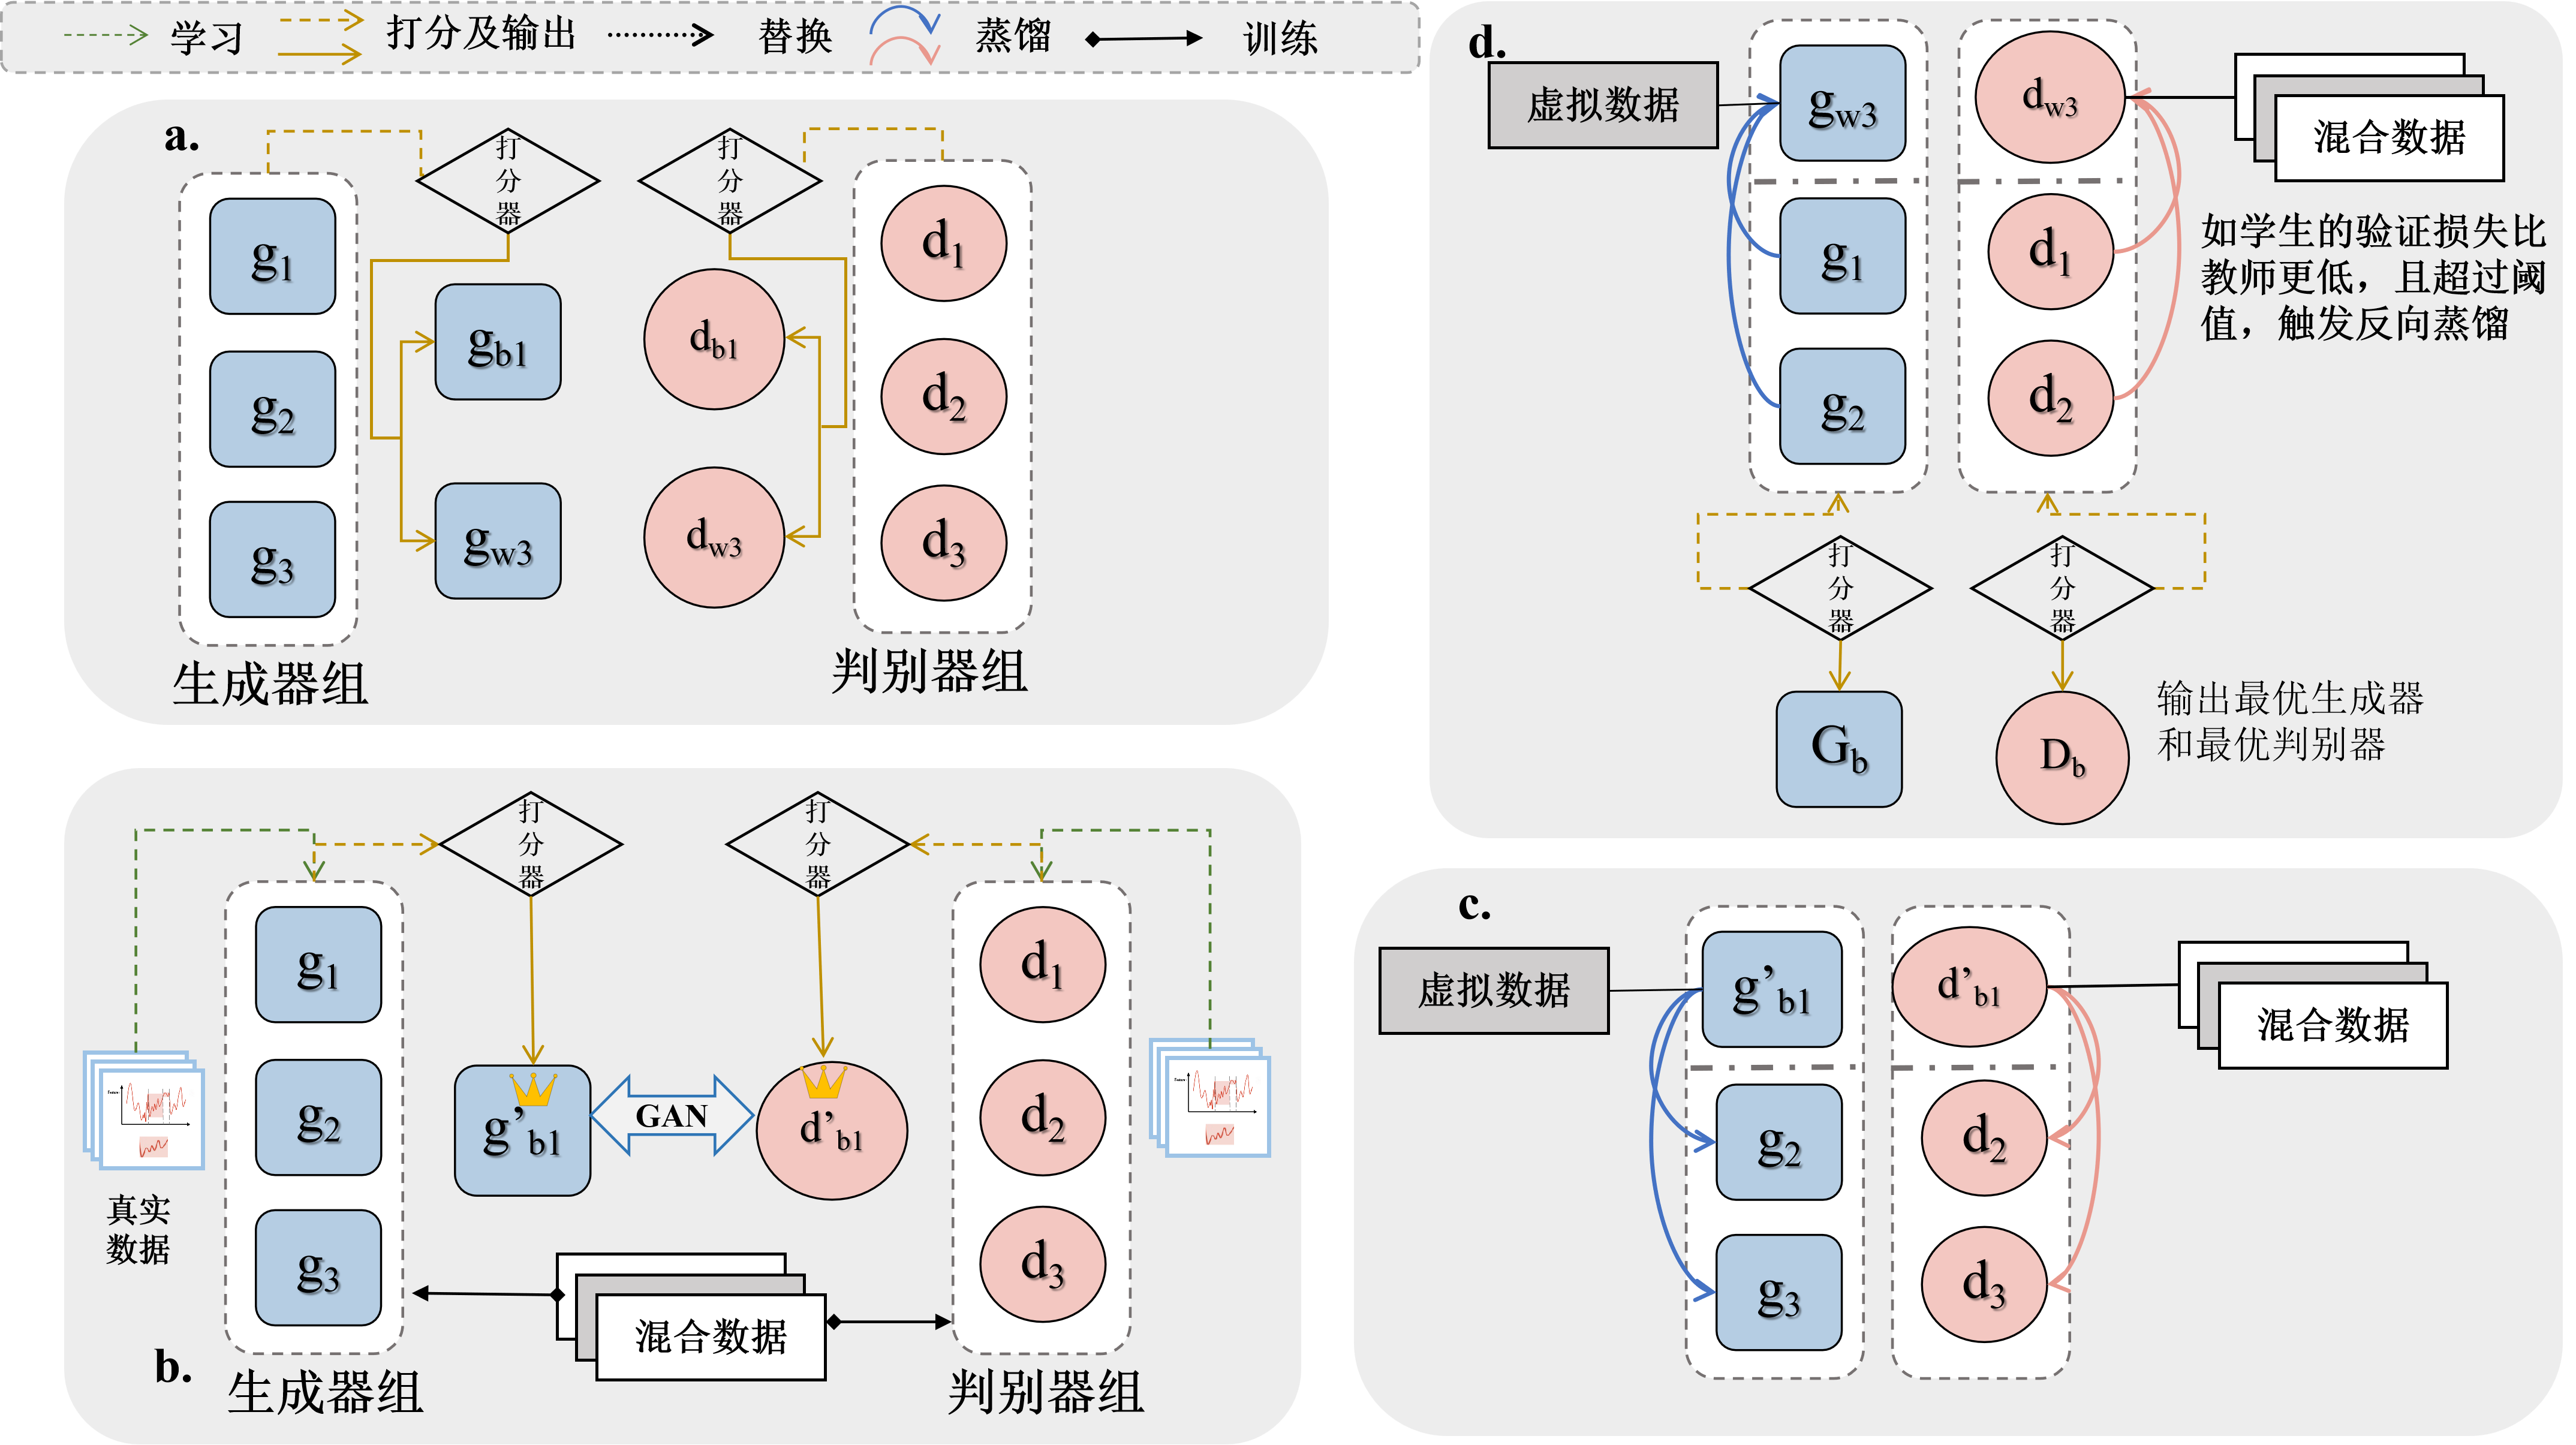
\includegraphics[width=0.8\textwidth]{figures/chap5/逆向对称.png}
    \caption{逆向师生蒸馏训练流程示意图}
    \label{fig:S2T-workflow}
\end{figure}

关于反馈阈值$\theta$的设定，本章采用动态自适应策略：以组内所有生成器在验证集上损失的均值$\bar{\mathcal{L}}$为基准，将阈值设定为$\theta = \alpha \cdot \bar{\mathcal{L}}$，其中$\alpha = 0.5$，即当最差成员的损失超过组内均值的1.5倍时触发蒸馏。在推理阶段，从训练完成后的生成器组中，选取在验证集上综合损失最小的生成器$G^\star_{\text{final}}$作为最终预测模型。这种动态阈值策略的优势在于：随着训练的推进，组内模型的整体损失逐渐降低，阈值也随之自适应调整，避免了固定阈值在训练早期过于宽松或后期过于严格的问题。

\subsection{带鱼短鱼机制趋势结构判别与策略映射}

本节进一步讨论时序结构识别结果如何转化为交易时机判断。四元分形事件用于描述结构事件是否出现，逆向师生蒸馏机制用于提升结构识别的稳定性，带鱼短鱼机制则用于判断已识别结构能否延续为具有交易意义的趋势波段。通过这一设计，本章将``结构是否出现''进一步转化为``结构是否具有交易意义''的判断，使模型输出能够服务后续交易执行优化与策略整合，并支撑交易流程中的交易时机判断。

在四元分形标签体系与逆向师生蒸馏机制的基础上，本章进一步引入``带鱼短鱼''机制，用于判断结构信号出现后能否延续为可交易的有效趋势。趋势跟随策略通常难以覆盖趋势启动初期的``鱼头''，也难以保留反转阶段的``鱼尾''，影响策略盈亏的关键，往往在于中段波段是否具有足够的延续性。基于这一考虑，本文将持续时间较长、终点价格优于起点价格的有效波段记为``带鱼''，将信号触发后较快反转、未形成有效收益的失败波段记为``短鱼''。其重点在于考察信号触发后的价格演化是否延续为有效趋势，而非评价信号形态本身是否完整。

这一划分为艾略特波浪理论中``有效浪''与``无效浪''的区分提供了可计算形式。将其纳入逆向师生蒸馏系统后，模型学习的对象不再只是局部结构是否出现，还包括该结构能否延续为有效趋势，从而为后续结构识别任务提供更稳定的监督信号。以指数平滑异同移动平均线金叉位置为波段起点 $t_s$，下一次反向信号（死叉）位置为波段终点 $t_e$，并以终点价格是否优于起点价格作为趋势有效性的判定准则：

\begin{equation}
\text{Label}_{[t_s, t_e]} =
\begin{cases}
\text{带鱼}, & \text{if } P_{t_e} > P_{t_s} \quad \text{（看涨波段）} \\
\text{短鱼}, & \text{if } P_{t_e} \leq P_{t_s} \quad \text{（看涨波段）}
\end{cases}
\end{equation}

对称地，在下跌趋势中：

\begin{equation}
\text{Label}_{[t_s, t_e]} =
\begin{cases}
\text{带鱼}, & \text{if } P_{t_e} < P_{t_s} \quad \text{（看跌波段）} \\
\text{短鱼}, & \text{if } P_{t_e} \geq P_{t_s} \quad \text{（看跌波段）}
\end{cases}
\end{equation}

这一机制可视为对四元分形事件划分的应用扩展。四元分形事件负责识别结构事件何时出现，``带鱼短鱼''则进一步判断这些结构是否真正转化为可持续的收益结构。若只看交叉或突破本身，模型容易学到大量假突破；而加入带鱼判定后，模型学习的对象同时包含``结构出现''与``结构是否走成''，从而更接近交易者真正关心的问题。

这一机制将``波段是否成功''转化为可观测、可训练的二元标签，解决了传统方法只能识别结构、不具备有效性验证机制的问题。从统计学角度来看，在本章所使用的15种期货品种的日频数据中，``短鱼''波段的数量通常占总波段数的60\%至75\%，呈现出典型的类别不平衡特征。这一分布特点进一步凸显了在模型训练中采用聚焦损失等不平衡处理策略的必要性。

从这一意义上看，本章最终形成的是一个“结构—有效性”两级标注框架：前层由 C/D/V/A 分形描述市场中的结构事件，后层由带鱼短鱼判定这些结构是否具备趋势持续性。这样处理既保留了波浪理论对结构的关注，也把无效信号过滤纳入可监督学习流程，为本章逆向师生蒸馏机制的训练与实验解释提供了更稳固的标签基础。更重要的是，该框架将``是否出现结构''与``是否值得据此交易''区分开来，使本章方法能够从结构识别进一步落到交易时机判断，而不是停留在一般分类任务。

\section{实验}

本章实验面向时序结构识别任务，检验逆向师生蒸馏学习方法在高噪声金融序列中是否能够提高结构事件识别的稳定性，并观察识别到的结构信号能否支撑交易时机判断。评价指标包括精确率、召回率、精确率与召回率调和平均值、混淆矩阵以及不同预训练模型对比，目的在于判断模型是否减少伪结构误判、保留有效结构信号，并为后续执行优化和策略整合提供更可靠的结构输入。因此，本章实验不是单纯比较分类器优劣，而是检验四元分形标注、逆向师生蒸馏和趋势有效性判别能否共同回应交易时机判断这一问题。

\subsection{实验数据集}
为验证基于四类分形模式的趋势识别方法及多智能体结构学习框架的有效性，本章选取中国商品期货市场具有代表性的15种主要期货品种作为研究对象，覆盖金属、农产品、能源化工及软商品等多个行业板块。数据集的构建目的在于检验模型对不同行情品种中时序结构的识别能力，因此实验不仅关注单个标签的分类结果，也关注结构事件在不同市场状态下的稳定性。所有数据均来自公开市场的日度行情，包含开盘价、最高价、最低价和收盘价等基础价格字段。本章进一步从开盘价、最高价、最低价和收盘价序列中构造短周期与长周期指数加权移动平均线（5指数加权移动平均线与120指数加权移动平均线）、价格变化率、实体宽度、上下影线比例等派生指标。在数据预处理阶段，首先剔除所有节假日与停牌日，对缺失数据点采用前向填充方式补全，并通过滑动窗口方式对部分派生特征进行平滑处理。四类分形结构标签基于本章提出的规则系统自动完成，最终形成的输入特征包含原始价格、技术指标、一阶变化率及多尺度结构信息。

\subsection{实验设计}
本章实验设计围绕两类目标展开：一是检验四元分形事件、逆向师生蒸馏机制与趋势有效性判别对时序结构识别稳定性的影响；二是说明这些结构信号能否服务于交易流程中的时机判断。因此，实验评价同时关注C/D/V/A四类结构事件的识别结果、不同模型预训练方式对结构边界的影响，以及逆向师生蒸馏机制对噪声误判和模式坍缩的缓解作用。

为保证实验结论能够同时反映识别性能与交易意义，本章在实验设计中同时设置结构事件识别评价和回测评价两个层次。其中，结构事件识别评价用于检验模型对C/D/V/A四类事件边界的识别能力，回测评价则用于检验上述结构事件是否能够进一步转化为交易时机判断。换言之，本节涉及的回测公式和交易指标属于实验设计中的验证口径，并不单独构成新的交易策略章节。

在特征工程层面，本章对输入特征进行了系统化的层次设计。第一层为基础价格特征，包括开盘价、最高价、最低价、收盘价四个原始字段；第二层为趋势敏感特征，包括5日指数加权移动平均线与120日指数加权移动平均线及其差值，用于捕捉短期与长期趋势的方向与强度；第三层为动量特征，包括指数平滑异同移动平均线的动量线、信号线与柱状线，以及价格的一阶变化率；第四层为K线结构特征，包括实体宽度（收盘价与开盘价之差的绝对值）、上影线长度、下影线长度及其比例关系。通过这种多层次的特征构建，模型能够同时获取价格的绝对水平、相对变化趋势、动量状态与微观结构信息，为后续的多任务学习提供了丰富的输入表示。

为量化评估四类分形结构标签体系与逆向师生蒸馏机制在实际交易中的表现，本章设计了基于日频价格序列的回测评估流程。策略每日仓位取值为+1（做多）、-1（做空）或0（中性/持有），由结构信号的预测方向直接决定。在单资产回测中，策略每日收益率计算方式为：

\begin{equation}
r_t^{\text{strategy}} = \text{pos}_{t-1} \cdot \left(\frac{P_t}{P_{t-1}} - 1\right) - \text{fee},
\end{equation}

其中$pos_{t-1}$为前一日仓位，$P_t$为第t日收盘价，fee为每笔交易的手续费。策略权益曲线以1.0为起点，通过逐日复利累乘计算：

\begin{equation}
\text{equity}_t = \prod_{i=1}^{t}\left(1 + r_i^{\text{strategy}}\right).
\end{equation}

本章采用以下评估指标：策略总累计收益率 $\text{TotalReturn} = \text{equity}_T - 1$；年化收益率 $\text{AnnualReturn} = \text{equity}_T^{252/T} - 1$；年化波动率 $\sigma_{\text{annual}} = \sqrt{252} \cdot \text{std}(\{r_t^{\text{strategy}}\})$；夏普比率 $\text{Sharpe} = (\bar{r}_{\text{annual}} - r_f) / \sigma_{\text{annual}}$；最大回撤 $\text{MDD} = \min_t\left(\text{equity}_t / \max_{i\le t}\text{equity}_i - 1\right)$；卡玛比率 $\text{Calmar} = \text{AnnualReturn} / |\text{MDD}|$。

在数据划分方面，本章采用时间序列的滚动窗口划分策略，以避免前视偏差。具体而言，将每个品种的历史数据按时间顺序划分为训练集（前60\%）、验证集（中间20\%）和测试集（后20\%）。验证集用于模型选择与超参数调优，测试集仅用于最终的性能评估与回测分析。所有评估指标均在测试集上计算，确保结果的客观性与可比性。

对比基线包括：GCA（多智能体对抗预训练模型）、GCA无内部知识共享版本（无内部知识共享的消融版本）、自注意力序列模型、门控循环单元、长短期记忆网络以及生成对抗网络六类具有代表性的预训练模型，涵盖生成式建模、序列建模与多智能体结构学习等不同范式。围绕分形事件识别任务（C、D、V、A），实验从两个层面评估模型的结构识别能力：一是逆向师生蒸馏机制与基线方法的总体比较，二是不同预训练模型对识别结果的影响。通过上述对比，可以观察逆向师生蒸馏机制在弱模型向强模型反向校正、波浪结构识别和局部伪结构过滤中的作用。

\subsection{结果分析与讨论}
本节从时序结构识别和交易时机判断两个层面解释实验结果。对于本章任务而言，准确率只能反映整体分类情况；精确率提升说明模型减少了伪结构误判，召回率提升说明模型能够捕捉更多真实结构事件，精确率与召回率调和平均值提升则说明模型在结构确认与信号覆盖之间取得更好平衡。对应到交易流程中，精确率关系到是否减少错误买入或错误卖出，召回率关系到是否遗漏有效趋势结构，因此这些指标共同反映了时序结构识别对交易时机判断的支持程度。

\begin{table}[htbp]
\centering
\caption{不同任务下基线方法与逆向师生蒸馏方法的性能对比}
\label{tab:s2t-performance}
\begin{tabular}{llcc}
\hline
\textbf{预测任务} & \textbf{指标} & \textbf{基线方法} & \textbf{逆向师生蒸馏机制} \\
\hline
\multirow{4}{*}{C} & 准确率  & 0.8814 & 0.8846 \\
                   & 精确率 & 0.2515 & 0.2572 \\
                   & 召回率    & 0.9498 & 0.9520 \\
                   & 精确率与召回率调和平均值        & 0.3977 & 0.4050 \\
\hline
\multirow{4}{*}{D} & 准确率  & 0.8859 & 0.9075 \\
                   & 精确率 & 0.2555 & 0.2920 \\
                   & 召回率    & 0.9138 & 0.8616 \\
                   & 精确率与召回率调和平均值        & 0.3994 & 0.4362 \\
\hline
\multirow{4}{*}{V} & 准确率  & 0.5664 & 0.4950 \\
                   & 精确率 & 0.4573 & 0.4242 \\
                   & 召回率    & 0.8175 & 0.9581 \\
                   & 精确率与召回率调和平均值        & 0.5865 & 0.5880 \\
\hline
\multirow{4}{*}{A} & 准确率  & 0.4724 & 0.4844 \\
                   & 精确率 & 0.4031 & 0.4082 \\
                   & 召回率    & 0.9555 & 0.9481 \\
                   & 精确率与召回率调和平均值        & 0.5670 & 0.5707 \\
\hline
\end{tabular}
\end{table}

从表\ref{tab:s2t-performance}与图\ref{fig:S2T-f1_bar}可以看出，逆向师生蒸馏机制在C与D两个方向切换类任务上均获得了稳定提升，其中D任务改善最为明显；在V与A任务中，模型则主要表现为召回率提升。这表明逆向师生蒸馏机制更有助于捕捉趋势切换与结构确认信号，同时在突破/跌破类事件中保留了更高的信号覆盖能力。图\ref{fig:S2T-cm_c}与图\ref{fig:S2T-cm_d}进一步给出了C、D任务的混淆矩阵结果，说明逆向师生蒸馏机制在关键时序结构识别中具有更好的判别效果；图\ref{fig:S2T-radarf1}则表明该优势具有一定的跨任务一致性。

\begin{figure}[htbp]
    \centering
    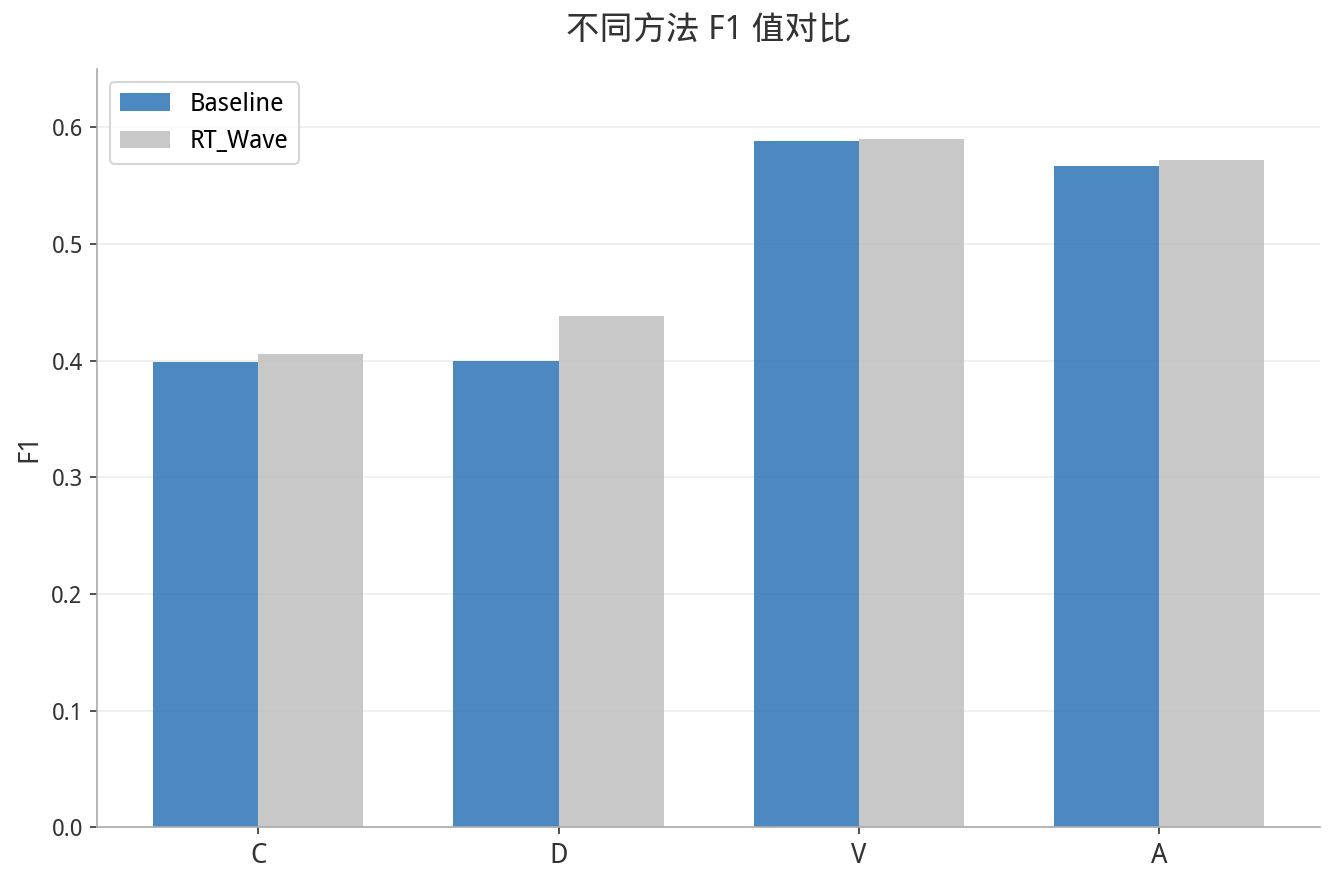
\includegraphics[width=1\linewidth]{figures/chap5/图4.5改.png}
    \caption{四类分形任务精确率与召回率调和平均值对比}
    \label{fig:S2T-f1_bar}
\end{figure}

\begin{figure}[htbp]
    \centering
    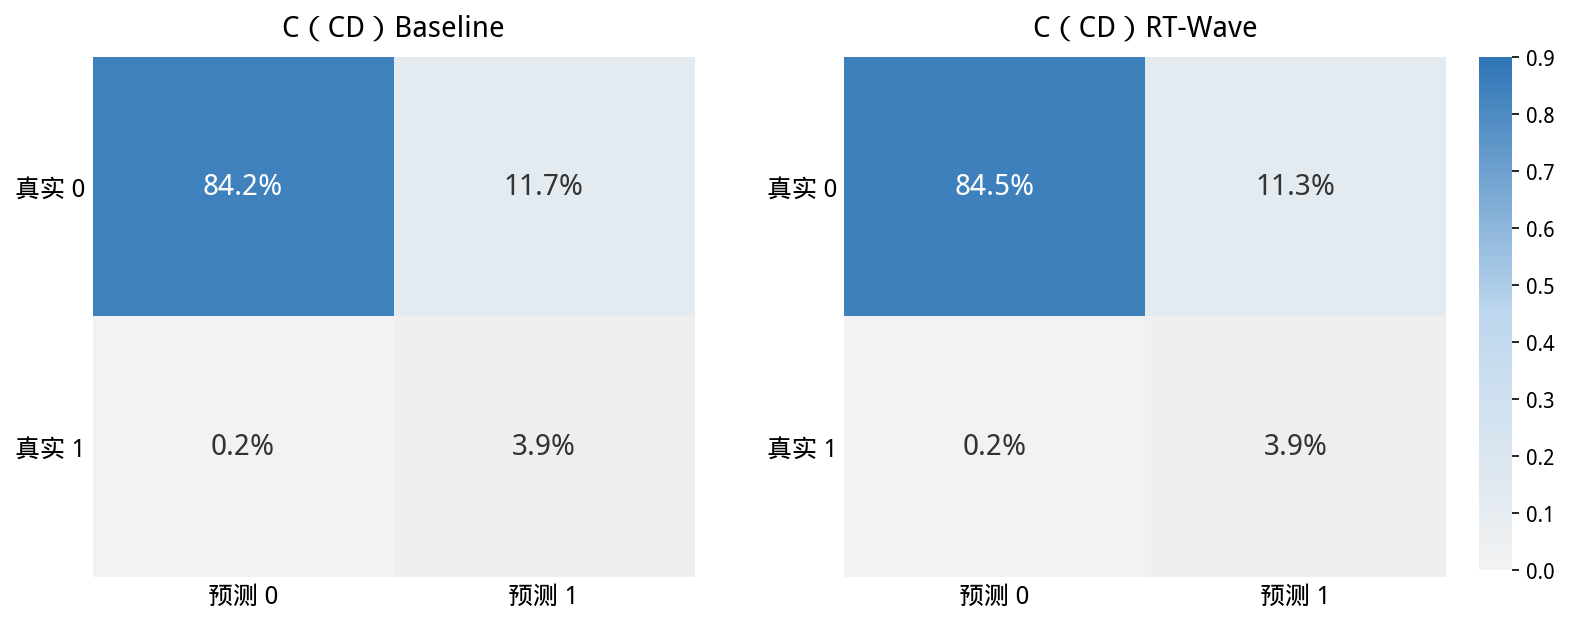
\includegraphics[width=1\linewidth]{figures/chap5/图4.6改.png}
    \caption{C 任务（看涨上穿）的混淆矩阵对比}
    \label{fig:S2T-cm_c}
\end{figure}

\begin{figure}[htbp]
    \centering
    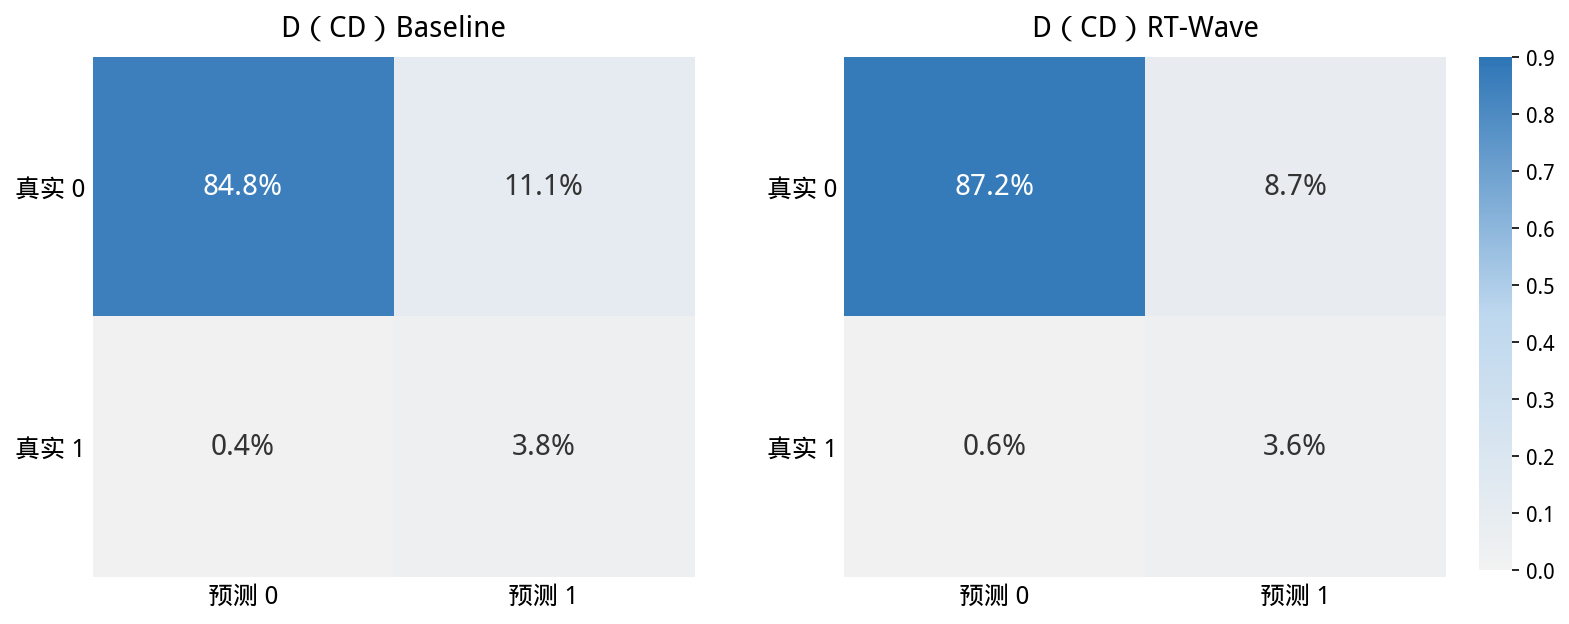
\includegraphics[width=1\linewidth]{figures/chap5/图4.7改.png}
    \caption{D 任务（看跌下穿）的混淆矩阵对比}
    \label{fig:S2T-cm_d}
\end{figure}

\begin{figure}[htbp]
    \centering
    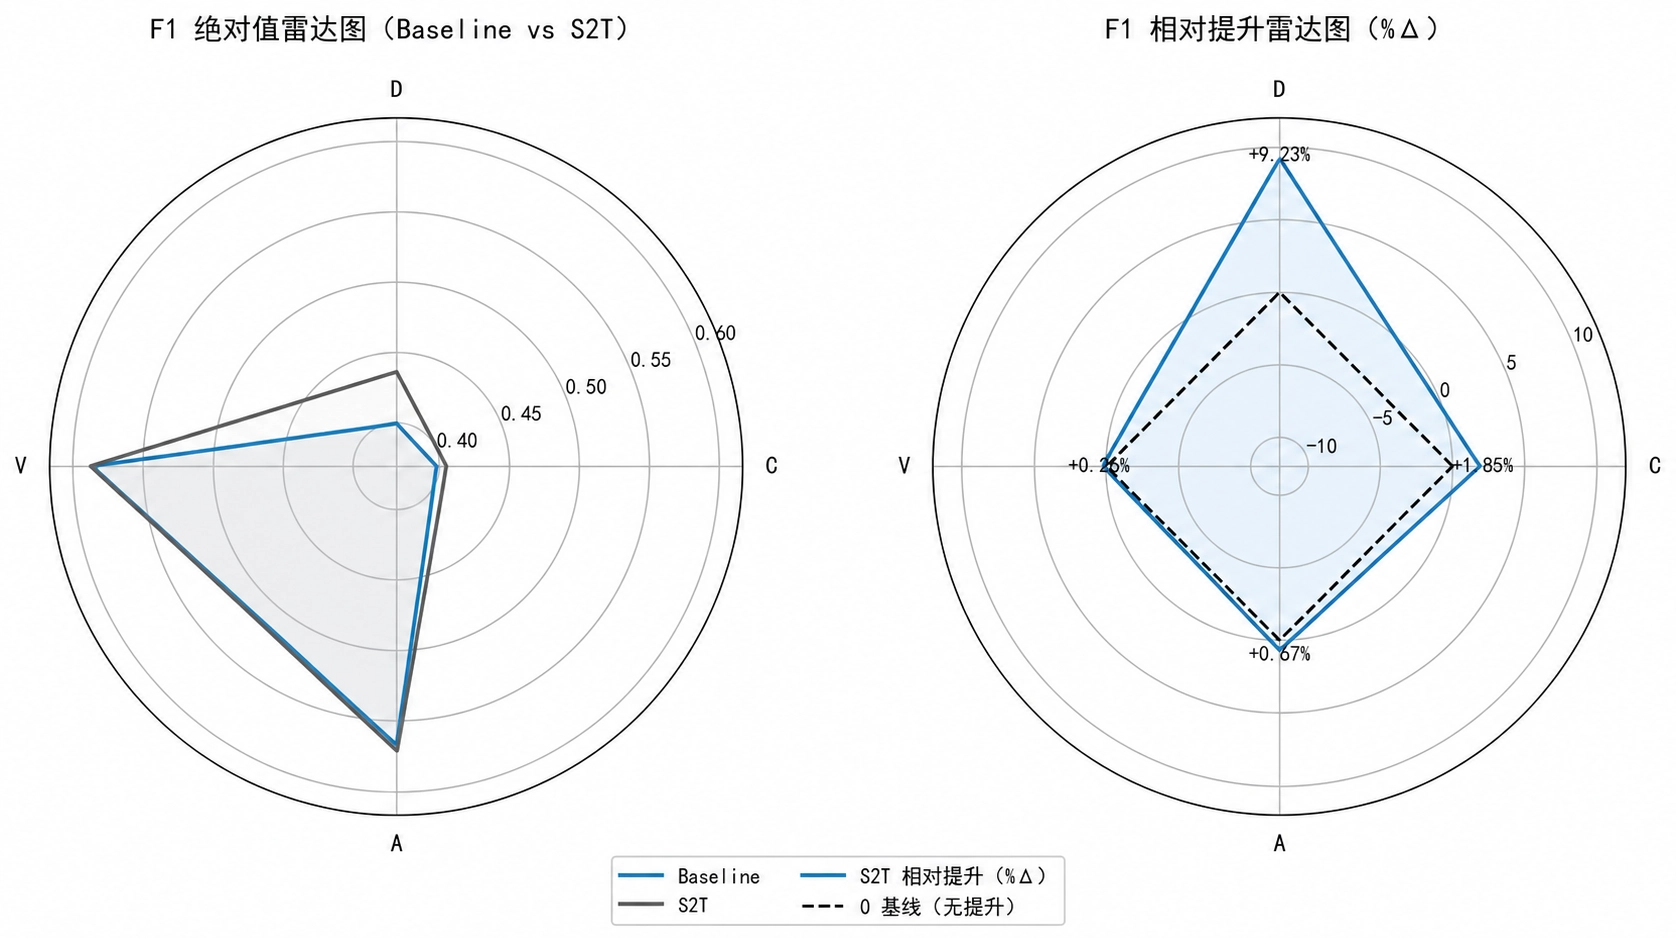
\includegraphics[width=1\linewidth]{figures/chap5/图4.8改.png}
    \caption{精确率与召回率调和平均值与相对提升雷达图}
    \label{fig:S2T-radarf1}
\end{figure}

\begin{figure}[htbp]
    \centering
    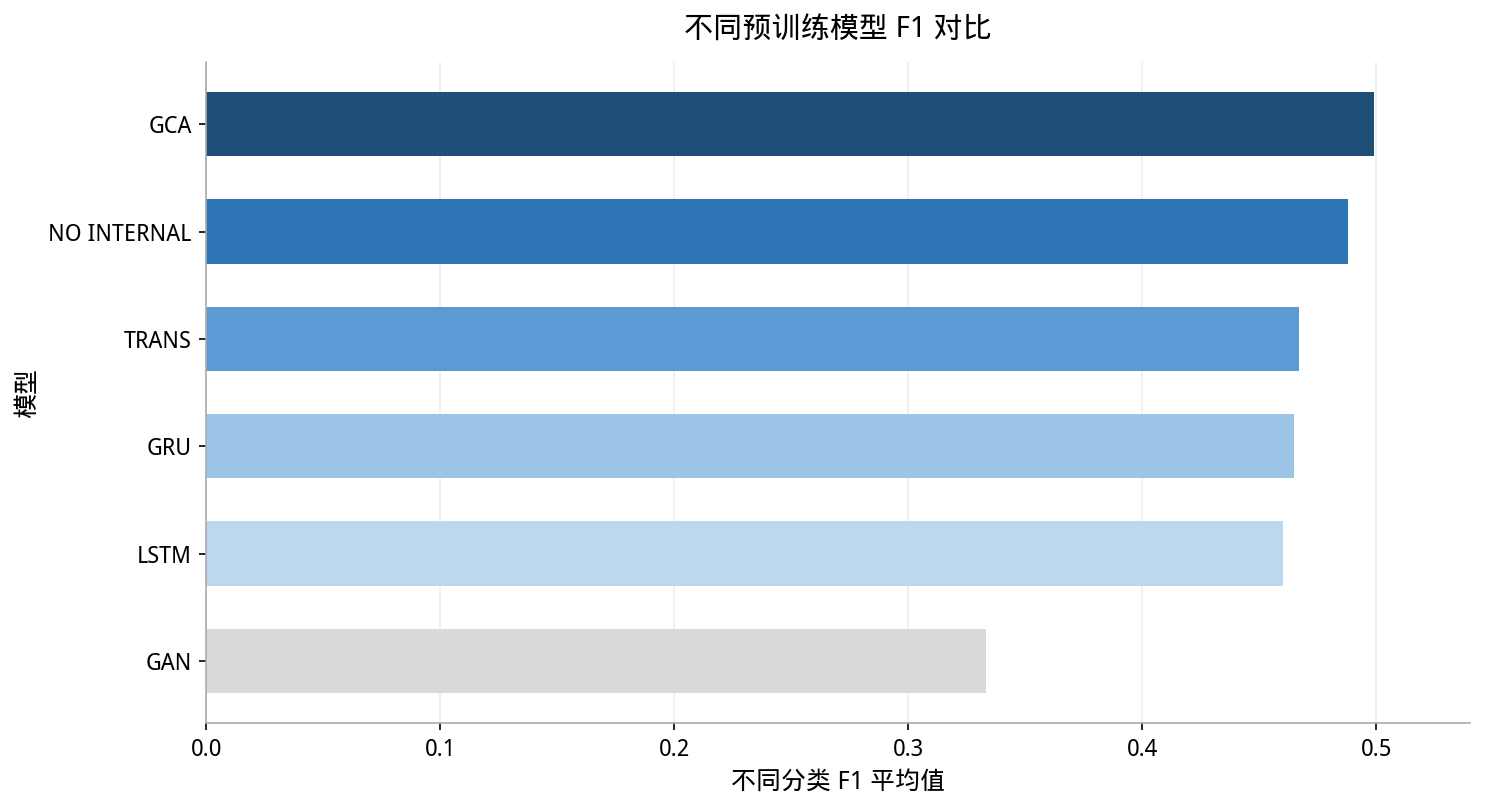
\includegraphics[width=1\linewidth]{figures/chap5/图4.9改.png}
    \caption{不同预训练模型平均精确率与召回率调和平均值对比图}
    \label{fig:S2T-models-F1}
\end{figure}

在预训练模型的对比实验中，从平均精确率与召回率调和平均值的柱状图\ref{fig:S2T-models-F1}可以看到，GCA在总体性能上位于最优水平，明显优于自注意力序列模型、门控循环单元、长短期记忆网络等常用时序模型，同时与GCA无内部知识共享版本拉开了可观察的差距。GCA无内部知识共享版本作为消融实验的对照组，移除了组内知识共享机制，其性能下降验证了多智能体内部协同对结构学习的贡献。进一步观察雷达图\ref{fig:S2T-models-radar}，GCA的优势具有明确的``结构一致性''特征：其在C与D两个方向切换类任务上呈现出更突出的精确率与召回率调和平均表现，同时在V与A两个突破/破位任务上也保持了相对更高且均衡的水平。相比之下，自注意力序列模型与长短期记忆网络虽然在部分任务上能够达到接近的精确率与召回率调和平均值，但在任务维度上呈现出更明显的``偏科''，导致整体平均效果无法超过GCA。

\begin{figure}[htbp]
    \centering
    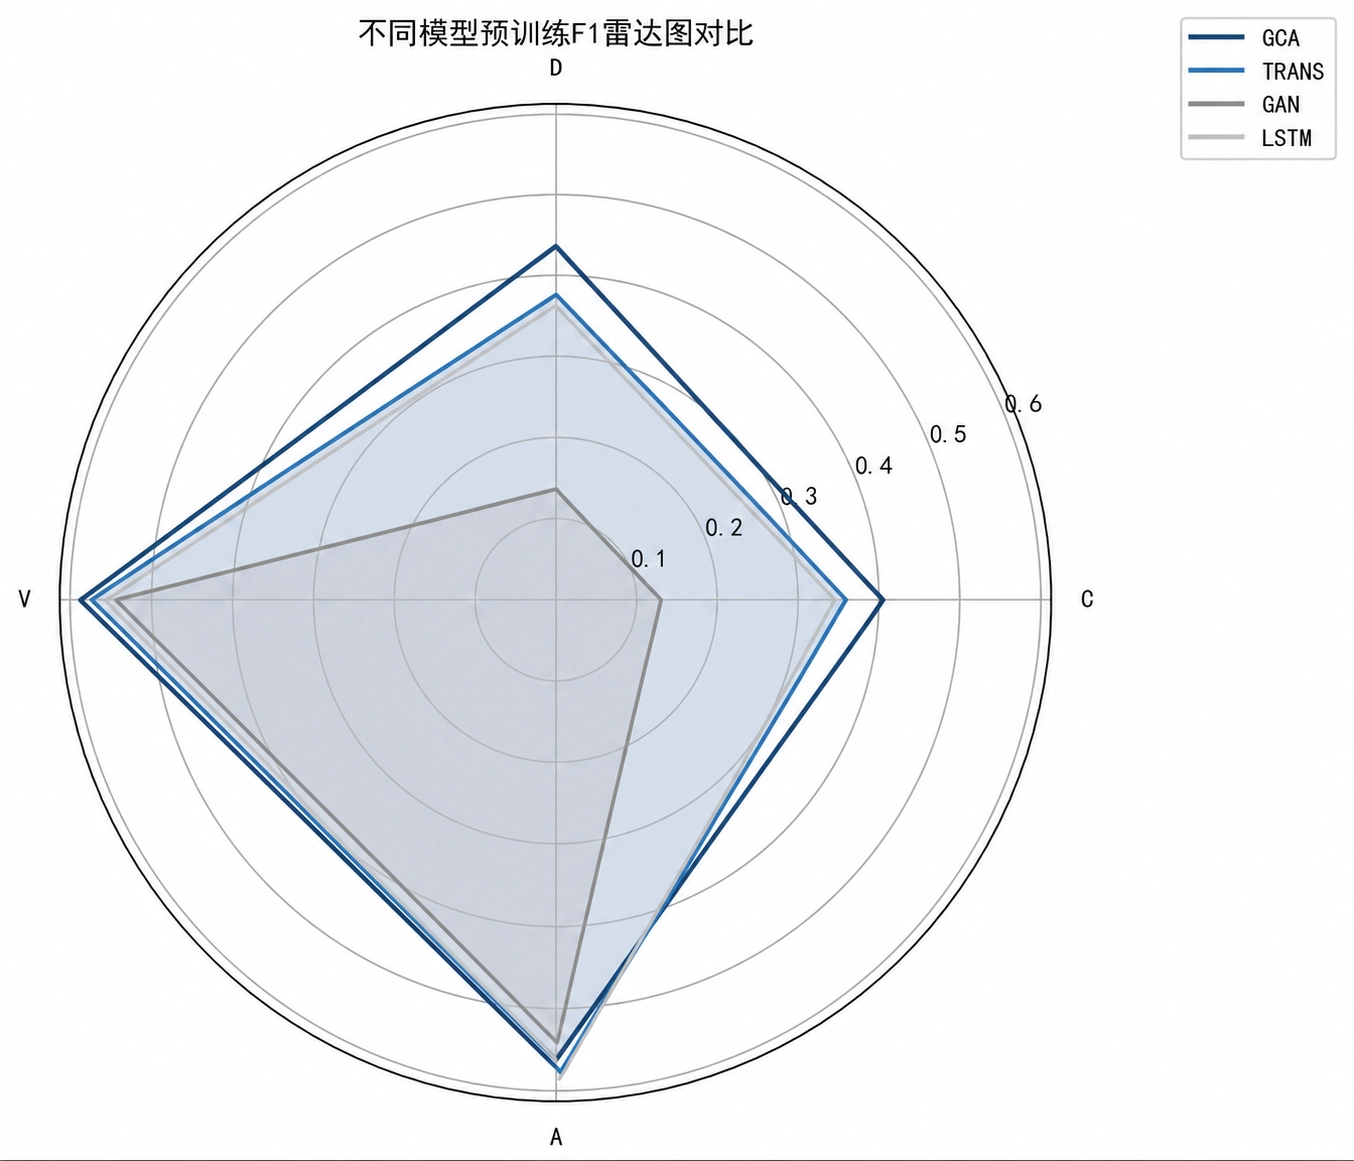
\includegraphics[width=0.75\linewidth]{figures/chap5/图4.10改.png}
    \caption{不同模型预训练精确率与召回率调和平均值对比雷达图}
    \label{fig:S2T-models-radar}
\end{figure}

\begin{figure}[htbp]
    \centering
    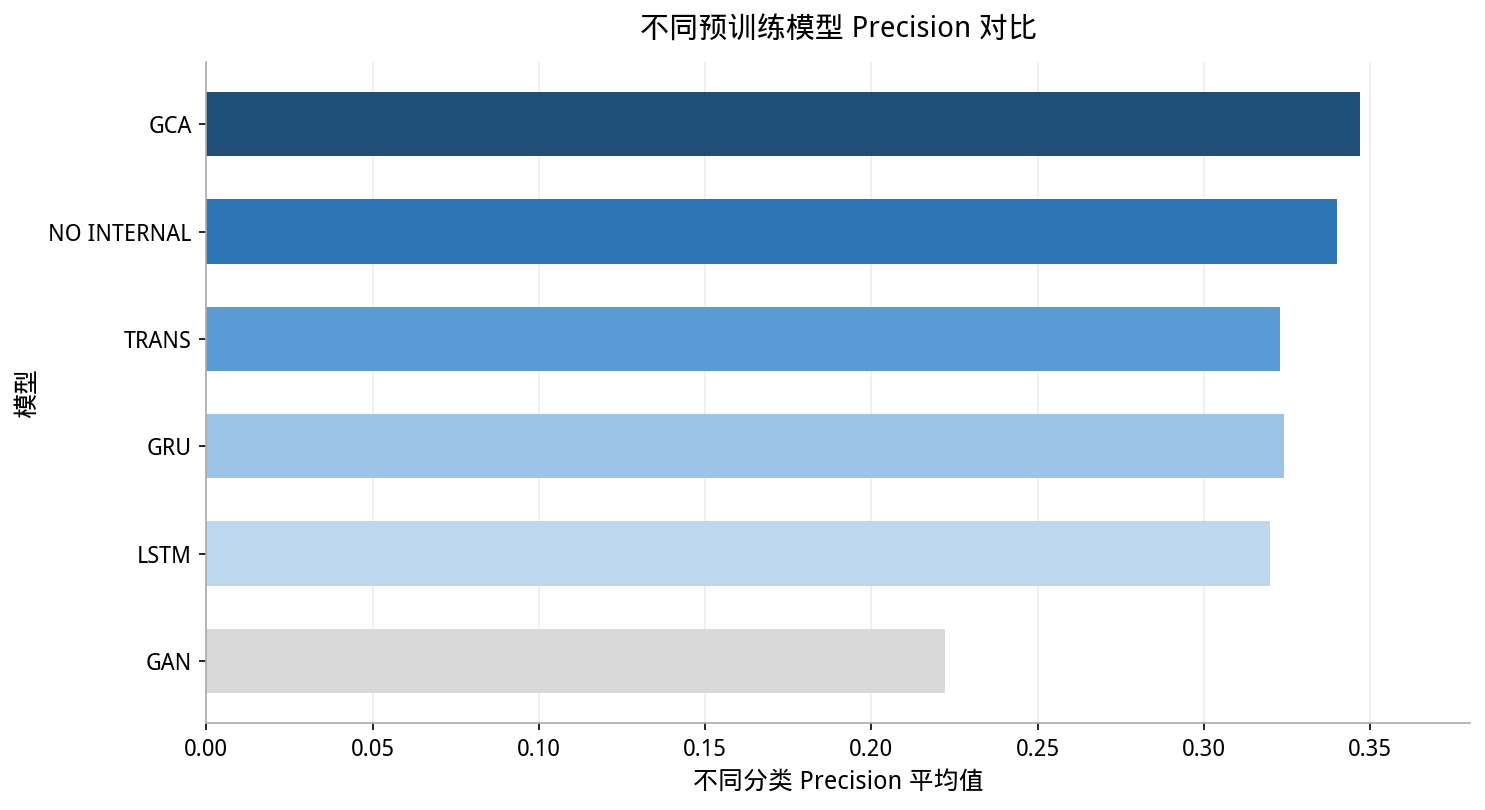
\includegraphics[width=0.75\linewidth]{figures/chap5/图4.11改.png}
    \caption{不同预训练模型平均精确率对比图}
    \label{fig:S2T-models-precision}
\end{figure}

\begin{figure}[htbp]
    \centering
    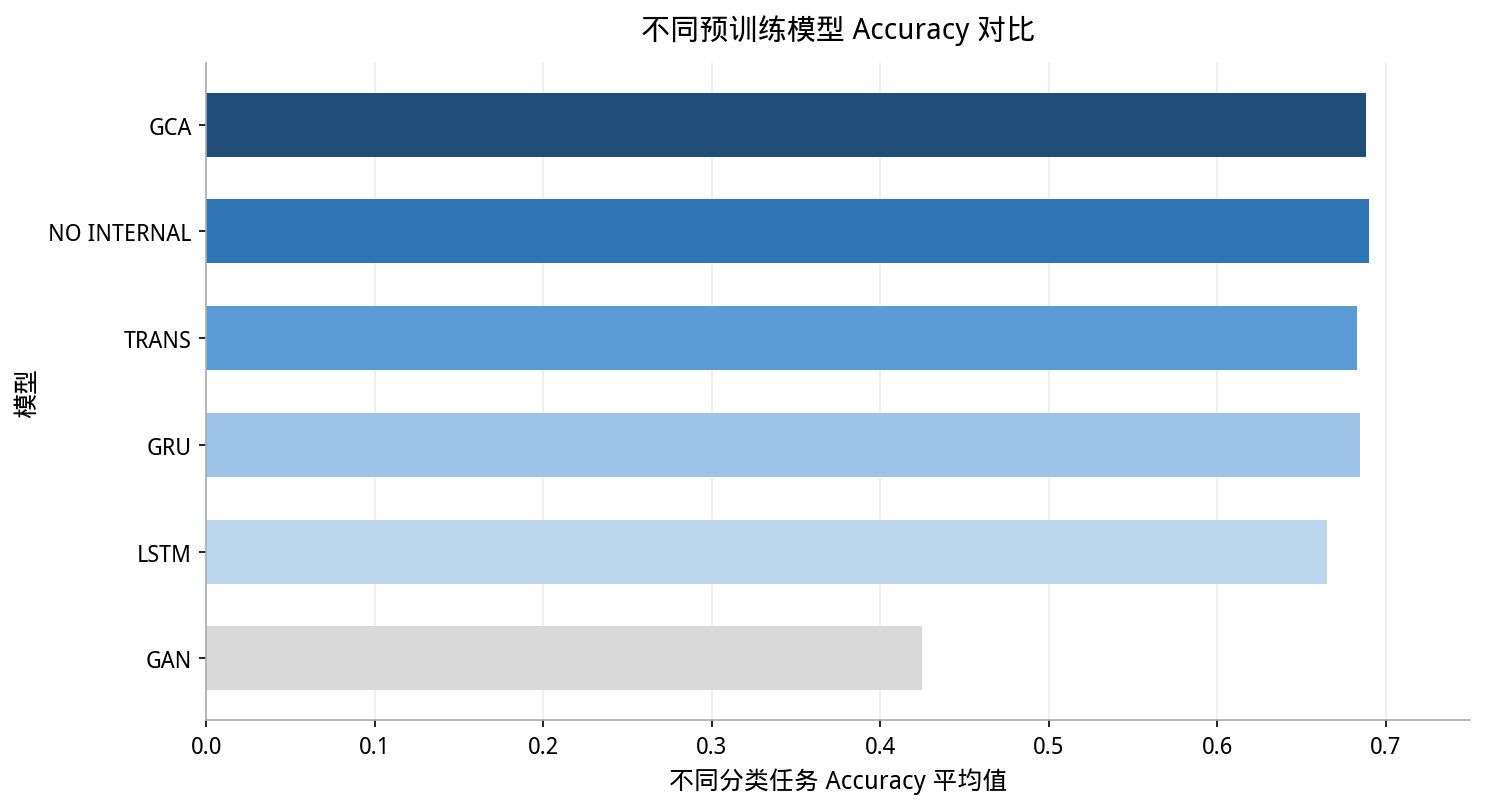
\includegraphics[width=0.75\linewidth]{figures/chap5/图4.12改.png}
    \caption{不同预训练模型平均准确率对比图}
    \label{fig:S2T-models-accuracy}
\end{figure}

图\ref{fig:S2T-models-precision}与图\ref{fig:S2T-models-accuracy}分别展示了不同预训练模型在平均精确率与平均准确率上的对比结果。整体来看，作为预训练配置的GCA在这两项指标上均保持较高水平，说明其在结构事件识别中具有较好的稳定性与均衡性。

本章实验显示，逆向师生蒸馏机制在部分任务上表现出相对优势。从知识蒸馏的理论视角来看，传统知识蒸馏可以看作一种相对静态的知识传递过程，学生模型被动拟合教师的平滑标签。而在金融时间序列这种极度非平稳、高噪声的环境中，固定的``强教师''极易对局部伪结构过拟合。逆向师生蒸馏机制对传统单向蒸馏方式作了调整，引入了由弱模型向强模型提供补充约束的训练机制。可以从训练过程的角度理解，这种机制可以理解为在多模型训练过程中引入了一种动态约束，使强模型在训练中参考弱模型所保留的较全局的结构信息，从而有助于缓解决策边界过于敏感以及模式坍缩问题。这与实验中D任务精确率从0.2555提升至0.2920的结果相吻合。

从金融分形结构的特征空间来看，四元分形事件在真实市场中呈现出典型的长尾分布与边界模糊性。逆向师生蒸馏机制通过多任务结构识别网络组的内部评分与交叉蒸馏，缓解模型在特征空间中过早趋同的问题。当最优模型试图利用特定的高频噪声捷径来降低训练损失时，逆向蒸馏促使其在训练中参考组内其他成员的分布信息，这种共识约束减弱了非平稳局部噪声带来的影响，学习到具有较强跨尺度稳定性的时序结构特征。此外，由于C/D分形依赖于指数平滑异同移动平均线等均线系统，该类标签在刻画市场结构时具有天然的滞后性偏差。本章通过引入基于K线实体突破的V/A信号，利用其价格行为的即时性对指数平滑异同移动平均线的滞后性进行补偿；同时，在多任务学习框架下，模型输入融合了多尺度特征与一阶动量变化率，使深度网络更可能学习到动量衰竭与结构反转的相关结构信息，这与由滞后识别向更早期结构判断的现象相一致。

从实验结果的局限性来看，V与A任务的精确率相对较低（均低于0.50），这反映了基于单根K线实体突破的V/A定义在高频场景下的固有噪声敏感性。具体而言，V任务的精确率从基线的0.4573下降至逆向师生蒸馏机制的0.4242，而召回率则从0.8175大幅提升至0.9581，这种精确率与召回率之间的权衡反映了逆向师生蒸馏机制在面对高频V/A事件时的策略倾向：模型更倾向于捕获尽可能多的真实结构信号，即使这意味着引入更多的假正例。在实际交易应用中，这种倾向可以通过后续的信号过滤模块加以修正，例如结合成交量确认或多周期一致性检验来剔除低置信度的V/A信号。

在消融实验的分析中，GCA无内部知识共享版本的性能下降幅度为理解模型内部协同机制的贡献提供了量化依据。移除组内知识共享后，模型在C任务上的精确率与召回率调和平均值下降约5\%，在D任务上下降约8\%，这一结果反映出组内蒸馏机制对于方向切换类事件的识别贡献相对更大。进一步分析发现，生成对抗网络基线模型在V/A任务上的表现相对较好，但在C/D任务上明显落后于GCA，这与生成对抗网络缺乏显式的结构化标签监督有关——生成对抗网络的生成器主要学习数据分布的整体统计特性，而非特定的结构转折模式。相比之下，GCA通过将对抗训练与结构化监督相结合，能够在保持分布拟合能力的同时增强对特定结构事件的判别精度。

从模型训练的收敛行为来看，逆向师生蒸馏机制在训练中期表现出一定的``震荡收敛''特征：由于反向蒸馏的周期性触发，强模型的验证损失可能出现短暂的上升波动，随后在正向蒸馏的驱动下重新下降。与传统单向蒸馏的单调收敛相比，这种训练扰动有助于缓解模型过早停留在局部最优附近的问题。在15个期货品种的实验中，约有11个品种在逆向师生蒸馏训练后期观察到了这种震荡收敛现象，且最终收敛值均低于未使用逆向师生蒸馏机制的对照组，进一步验证了反向蒸馏机制在优化景观中的探索作用。

在未来的工作中，可以考虑引入多周期确认机制或自适应阈值策略，以进一步提升V/A事件识别的精确率。此外，当前实验仅在日频数据上进行验证，将四元分形事件框架扩展至分钟级或tick级数据时，可能需要对分形事件的定义参数进行重新校准。另一个值得探索的方向是将四元分形标签体系与注意力可视化技术相结合，通过分析模型在做出结构识别决策时关注的时间窗口位置与特征维度，进一步提升框架的可解释性，为交易策略的设计提供更直观的依据。


\section{本章小结}

本章围绕对冲基金交易决策流程中的时序结构识别环节，提出面向时序结构识别的逆向师生蒸馏学习方法，重点服务于交易时机判断问题。与第2章侧重投资组合管理、第3章侧重高维金融因子建模不同，本章进一步关注价格路径中的趋势结构、结构边界与有效波段，尝试将传统波浪理论中的主观形态判断转化为可监督、可检验的时序结构识别任务。由此，波浪结构识别在本章中承担时序结构识别的具体实现功能，其目标是为后续交易执行优化和策略整合提供更可靠的结构信号。

在方法层面，本章工作主要体现在三个方面。第一，通过四元分形事件标注方法，将复杂的波浪形态量化为C、D、V、A四类结构事件，其中C/D基于指数平滑异同移动平均线动量指标捕捉宏观趋势转折，V/A基于K线实体突破捕捉微观结构波动，二者在时间尺度上形成互补，共同构成了面向时序结构识别的结构化标签体系。第二，逆向师生蒸馏机制对单向知识传递方式作了调整，通过动态监控与反向校正，使强模型在训练中参考弱模型保留的较全局结构信息，缓解多任务结构识别中的类别不平衡、局部伪结构过拟合与决策边界锐化问题。第三，引入``带鱼短鱼''机制对趋势的延续与反转提供较清晰的数学界定，将传统波浪理论中``有效浪''与``无效浪''的定性判断转化为基于价格终点与起点比较的二元判定，使模型能够进一步判断结构信号是否延续为具有交易意义的趋势波段。

在实验层面，本章在15种中国商品期货品种的日频数据上进行了验证。实验结果显示，逆向师生蒸馏机制在C与D两个核心任务上取得了稳定的精确率与召回率调和平均值提升，其中D任务的精确率与召回率调和平均值提升幅度超过9\%，精确率提升超过14\%。在预训练模型的对比实验中，作为预训练配置的GCA在平均精确率与召回率调和平均值、精确率与准确率三个维度上均优于自注意力序列模型、门控循环单元、长短期记忆网络等常用基线模型，说明协同训练在金融结构化建模中具有一定作用。混淆矩阵分析进一步揭示了逆向师生蒸馏机制在降低假正例率方面的优势，尤其在D任务中，模型对看跌结构转折的判别精度得到了实质性改善。上述结果说明，本章方法不仅改善了局部分类指标，也提高了时序结构信号对交易时机判断的支持能力。

尽管本章取得了一定的实验结果，但仍存在若干局限性与待改进之处。第一，V与A任务的精确率仍然偏低，这与基于单根K线实体突破的定义在高频场景下的固有噪声敏感性有关，未来可通过引入多周期确认机制或自适应阈值策略加以改善。第二，当前实验仅在日频数据上进行验证，将四元分形事件框架扩展至更高频率的数据时，分形事件的定义参数可能需要重新校准。第三，反向蒸馏的触发阈值目前采用的是基于组内均值的动态策略，未来可以探索更加精细化的自适应触发机制，例如基于梯度信息或特征空间多样性指标的动态调整策略。第四，本章主要关注结构识别性能指标，尚未将四元分形事件结构信号与实际交易策略的盈亏表现进行系统关联分析，这将在后续章节中通过交易执行优化与策略整合模块的结合加以完善。

本章对应交易决策链条中的第三个环节，即在明确资产配置和因子依据形成之后，判断交易时机判断。通过四元分形事件、逆向师生蒸馏机制和带鱼短鱼机制，本章形成了从结构事件标注、结构边界校正到趋势有效性判别的分析路径。第5章将在此基础上讨论结构信号确认后的交易执行路径优化，第6章则继续面向最终交易判断讨论策略整合问题。
 
     \chapter{面向交易执行优化的孪生对抗自体再生方法}

% 兼容局部浮动体分组控制：若主文件已加载 placeins，则使用正式 \FloatBarrier；若未加载，则不影响编译。
\providecommand{\FloatBarrier}{}

\section{问题的提出}

\subsection{交易执行中的滑点风险与市场冲击成本}

% 在完成了从宏观资产配置（第 2 章）、中观因子建模（第 3 章）到微观形态分类（第 4 章）的预测体系构建后，本章将研究焦点下沉至算法交易的最终执行环节——VWAP（成交量加权平均价格）滑点控制\cite{almgren2001optimal,madhavan2002vwap}。在现代高频交易环境中，预测精度与经济价值之间往往存在非单调性悖论：一个在统计误差上表现优异的模型，若在流动性枯竭或趋势反转的关键节点发生方向性误判，可能放大执行滑点与市场冲击成本\cite{berkowitz1988total,cartea2015algorithmic}。

在完成投资组合管理、高维金融因子建模与时序结构识别之后，交易系统已经分别形成了资产配置对象、因子依据和时机判断。然而，这些信号只有进入真实下单路径后，才能转化为可实现收益。本章进一步进入对冲基金交易决策流程中的交易执行优化环节，重点讨论交易执行路径如何优化的问题\cite{almgren2001optimal}。交易执行优化并不是前序模型的附属步骤，而是决定模型信号能否在市场摩擦、流动性约束和冲击成本条件下落地的独立环节。成交量加权平均价格作为机构投资者最广泛采用的执行基准之一，其核心目标在于将大额订单的实际成交均价控制在市场成交量加权均价附近，从而最小化对市场价格的冲击并降低信息泄露风险。对本文而言，成交量调度不是单纯的执行技巧，而是检验前序资产配置、因子依据和时序结构信号能否在真实市场中稳定落地的关键接口：一旦订单时间分布与市场流动性状态发生错配，前序模型形成的交易判断就可能在执行层转化为滑点、冲击成本和异常回撤。因此，本章将成交量加权平均价格执行作为具体场景，研究如何通过孪生对抗自体再生方法优化执行路径、过滤异常信号并降低执行偏差，使交易执行优化成为连接模型信号与真实成交结果的关键环节\cite{madhavan2002vwap}。

在现代高频交易环境中，预测精度与经济价值之间往往存在非单调性悖论：一个在统计误差上表现优异的模型，若在流动性枯竭或趋势反转的关键节点发生方向性误判，可能放大执行滑点与市场冲击成本。这一悖论的根源在于，统计损失函数与经济损失函数之间存在结构性错位。实证研究表明，交易成本的真实构成远比表面的买卖价差复杂，隐性成本往往占据主导地位\cite{berkowitz1988total}。在此背景下，如何在预测精度之外纳入执行成本与流动性约束，成为算法交易系统设计的重要问题。Cartea 与 Jaimungal 在随机控制框架下系统论证了执行算法的设计需将市场状态的动态反馈纳入优化目标，静态的预设执行计划在非平稳市场条件下将面临严重的次优性\cite{cartea2015algorithmic}。

从市场微观结构角度看，滑点并不是由单一价格误差造成的，而是买卖价差、订单簿深度、信息不对称与短时流动性共同作用的结果。市场微观结构综述表明，交易制度、报价机制和订单流结构会直接影响成交价格的形成过程\cite{Ananth2000Market}。进一步的实证研究也说明，市场微观结构变量不仅决定交易成本的大小，还会改变交易策略在不同市场状态下的可执行性\cite{hasbrouck2007empirical}。因此，对成交量加权平均价格执行而言，关键并不是在任意时点都追求更低预测误差，而是在有限时间窗口内识别哪些流动性片段更适合承接订单。流动性交易理论指出，执行者需要在等待流动性与立即成交之间权衡，否则容易将大额订单暴露为额外冲击成本\cite{huberman2005optimal}。

进一步看，成交量加权平均价格执行并不是单纯的价格预测问题，而是一个同时受到成交量分布、订单拆分路径与市场微观结构约束的序列决策问题。为避免在问题提出部分过早展开公式推导，本节先从交易含义上说明其核心关系：执行者需要在给定总订单量和有限执行窗口内，将订单量分配到不同时间片，并使实际执行均价尽量贴近市场成交量加权平均价格。若订单切片与真实成交量分布不匹配，执行均价就会偏离基准价格，形成滑点损失；若这种偏离在非平稳行情中持续扩大，前序模型形成的交易信号就可能在成交层面被抵消。相应的成交量加权平均价格、执行量约束、实际成交均价与滑点损失等形式化表达，将在5.3.4节结合执行层修复目标集中给出。算法交易研究也指出，执行算法的价值取决于信号、成本和市场反馈之间的协调，而不是单独依靠某一类预测器完成全部决策\cite{2014Algorithmic}。

基于上述分析，本章将交易执行优化中的关键问题凝练为：如何把前序形成的交易信号转化为稳定的订单执行路径，如何在成交量预测误差、流动性错配和市场冲击之间建立动态约束，以及如何在候选执行信号退化时及时触发校验与修复。也就是说，本章方法需要真正回应的不是“能否预测成交量”，而是“能否在预测成交量—执行路径—滑点控制—崩溃修复之间形成可运行的闭环”。后文提出的孪生对抗自体再生方法正是围绕这一闭环展开。

\subsection{现有执行基准的结构性困境}

从交易执行优化视角看，现有执行基准的局限并不仅在于成交量曲线预测不够精确，而在于其通常缺乏对执行偏差、流动性错配和异常滑点的独立识别能力。静态成交量曲线假定历史成交分布可以为未来下单路径提供稳定参考，但真实市场中的流动性峰谷、突发冲击和参与者行为变化会不断改变执行环境。当执行器仍按固定模板下单时，上游资产、因子和时序结构信号可能在成交层被转化为价格冲击、成交滞后和滑点扩散。因此，本节讨论的结构性困境，本质上是现有执行框架缺少对执行路径的动态校验、异常过滤和持续调整能力。孪生对抗自体再生方法的引入，正是为了使执行系统能够在候选信号进入真实下单路径前完成校验与再平衡，从而服务于交易执行路径优化任务。

由此，本章的问题提出可以进一步归纳为三点：第一，执行层需要将前序信号映射为可执行的订单时间分布，而不能只保留离线预测结果；第二，执行模型需要识别成交量预测与真实流动性之间的偏离，避免订单集中落入不利时间片；第三，当模型组内出现同步退化或局部对抗失衡时，需要通过自体再生机制恢复执行系统的差异化校验能力。上述三点分别对应后文的动态调度器、孪生校验结构和跨组修复流程。

传统成交量加权平均价格算法以历史成交量分布为主要依据，其优势在于规则清晰、易于执行，但这一设定也意味着执行路径较容易受到历史均值曲线的约束。相关研究已经从竞争性分析角度讨论了在线决策在未知环境中的基准参照问题，为理解静态执行基准的局限提供了理论背景\cite{kakade2004competitive}。在真实市场中，成交量峰谷、订单簿深度和短时冲击会随市场状态变化而快速调整，执行器若缺少实时校验环节，就可能在低流动性阶段被动成交，或在价格不利区间放大交易冲击。

这一问题在高频交易环境下更加明显。市场微观结构研究表明，高频成交过程中的报价调整、订单到达和流动性供给会显著改变短周期价格形成机制\cite{goodhart1997high}。因此，执行基准不能只被理解为一条平均成交量曲线，而应被理解为一个需要随成交环境持续校验的动态参照系。已有改进成交量加权平均价格的研究也说明，仅依赖静态曲线难以充分适配真实日内成交形态，执行路径需要结合市场状态进行修正\cite{bialkowski2008improving}。这为本章后续引入动态调度器提供了直接动因。

与此同时，现有执行模型还面临预测精度与经济价值不一致的问题。早期关于预测评价的研究已经指出，统计精度提升并不必然意味着经济价值提升\cite{leitch1991economic}。对应到交易执行任务中，均方误差较低的成交量预测模型，并不一定能够降低滑点和冲击成本；真正决定执行质量的，往往是关键时间片上的流动性识别、异常成交过滤和转折状态下的路径调整能力。因此，本章关注的不是单纯降低成交量预测误差，而是使执行模型能够识别何时应当信任预测、何时应当降低敞口或触发自体再生。

从模型结构看，生成式和多模型方法为刻画复杂市场状态提供了新的工具，但也带来模型同步退化和局部共识幻觉的风险。多生成器生成对抗网络的研究表明，多个生成主体可以扩展样本模式覆盖范围，但不同主体之间仍需要有效的差异化约束和稳定训练机制\cite{ghosh2018multi}。若执行系统只叠加多个候选预测器而缺少独立校验机制，多个模型可能在同一类异常行情中同时失效。孪生对抗自体再生方法的核心作用，正是通过复制、配对与分化过程保留候选模型之间的可比较性，并在偏离累积到阈值时触发替换和短程修复，避免执行路径被单一退化信号长期主导。

综上，现有执行基准的结构性困境并不是单一预测精度不足，而是静态基准、经济价值错位和模型退化风险共同作用下形成的执行层稳定性问题。后文将围绕这一问题，进一步说明孪生对抗自体再生机制如何在执行前校验、异常过滤和动态调度中发挥作用。



\section{相关工作}

成交量加权平均价格执行优化的相关研究，通常围绕成交量预测、最优执行、市场冲击控制与执行路径校验展开。已有研究在执行基准设计、成交量曲线建模和市场状态表征方面积累较多，但对候选执行信号进入真实下单路径前的独立校验、异常过滤与动态再平衡讨论仍相对不足。因此，本节不再只围绕单一执行基准的精度展开，而是结合执行基准、预测价值错位、市场状态表征、生成式金融序列建模、模型互校验和多智能体系统等研究，说明孪生对抗自体再生方法的引入背景。

从执行基准研究看，成交量加权平均价格之所以被广泛采用，是因为它能够把大额订单拆解为与市场成交节奏相匹配的时间路径，并为交易成本评价提供相对稳定的参照。相关研究从理论层面讨论了成交量加权平均价格执行策略在特定市场冲击假设下的最优性条件，为理解该类基准的适用前提提供了基础\cite{kato2014vwap}。不过，这种最优性通常依赖于成交量分布、价格冲击函数和流动性状态的稳定假设；一旦日内成交结构发生偏移，单纯跟随历史均值曲线就可能放大滑点风险。进一步的最优性研究也表明，成交量加权平均价格执行并不是脱离约束条件的普遍最优策略，其有效性需要结合市场冲击、成交量过程和执行约束共同理解\cite{kato2016optimality}。因此，第五章关注的重点不是重新证明成交量加权平均价格基准本身的有效性，而是讨论执行系统如何在基准失效风险出现时进行动态校验和路径修正。

从成交量预测研究看，日内成交量比例并非完全随机，仍可通过历史成交形态、市场状态和短周期价格信息进行建模。近期关于日内成交量估计的研究表明，成交量曲线预测可以为订单拆分和执行节奏调整提供信息基础\cite{lee2024ive}。但是，对本文而言，成交量预测只是执行优化链条中的一个环节。即使预测曲线在均值意义上较为准确，关键时间片上的局部偏差仍可能造成集中成交、冲击成本上升或执行滞后。金融时间序列的经验事实也提示，收益分布、波动聚集和厚尾特征会使局部市场状态偏离常规均值假设\cite{Cont2001Empirical}。因此，孪生对抗自体再生方法并不只追求成交量预测误差最小化，而是进一步关注候选执行信号在进入下单路径前是否需要经过独立校验和再平衡。

从预测价值与执行价值的关系看，金融预测结果在统计指标上的改善并不必然转化为执行绩效改善。在非平稳市场中，预测模型的样本外表现和经济价值往往会随评价窗口、市场状态和交易成本假设变化而改变\cite{rossi2021forecasting}。这意味着执行模块不能把上游预测结果视为稳定输入，而需要在进入成交路径前重新判断其成本敏感性和风险暴露。进一步地，面向交易目标的训练研究也提示，若损失函数不能反映实际经济后果，模型可能在统计精度提升的同时放大执行端偏差\cite{zhou2024two}。因此，本章把预测输出视为待校验的候选信号，而不是直接下单依据。

从市场状态表征看，深度时序模型和订单簿建模方法增强了系统对短周期流动性、订单流不平衡和价格微结构的刻画能力。多变量时序预测研究说明，跨变量依赖和时间选择信息能够帮助模型识别不同阶段的状态变化\cite{lim2021temporal}。这类方法为执行系统理解市场状态提供了上游表征基础，但仍主要服务于预测任务；对于第五章而言，更关键的是将状态信息转化为下单路径中的校验、过滤与修复机制。以限价订单簿深度学习建模为代表的研究说明，深度模型能够从盘口形态中提取对短期价格变动有用的结构信息\cite{zhang2019DeepLOB}。这类研究为执行层理解市场微观结构提供了重要工具，但其目标通常仍偏向价格方向预测或状态识别。交易执行优化还需要进一步回答：当候选信号与真实流动性不一致时，系统如何发现偏离、如何过滤异常信号，以及如何避免退化模型持续主导下单路径。

从生成式金融序列建模看，对抗生成框架为刻画复杂数据分布提供了重要工具。生成对抗网络通过生成器与判别器之间的博弈过程学习数据分布，为金融场景中的序列生成和分布模拟提供了基础方法参照\cite{goodfellow2014generative}。不过，执行优化并不只需要生成“看起来合理”的市场路径，还需要判断这些路径是否会误导真实下单行为。面向金融时间序列的生成式研究进一步说明，生成模型可以在一定程度上复现收益序列的统计特征，为压力场景构造和样本扩展提供可能\cite{wiese2020quant}。这类研究对执行优化有启发意义，但若缺少执行前校验，生成样本中的局部偏差仍可能被下游调度器放大为实际滑点。

围绕多模型对抗与市场情景模拟的研究，也为本章的孪生校验思想提供了间接参照。多判别器生成框架通过引入多个判别视角增强对生成样本的约束，说明单一判别器并不总能充分识别复杂样本空间中的偏差\cite{nguyen2017dual}。金融市场生成器相关研究则从市场冲击和压力情景角度讨论了生成模型在金融模拟中的作用，为理解极端执行环境下的候选路径退化提供了补充视角\cite{kondratyev2019market}。这一视角说明，执行优化中的生成式建模不能停留在样本扩展层面，还需要进一步检验候选路径在流动性收缩、冲击成本放大和成交量分布偏移条件下是否仍具有可执行性。换言之，生成模型提供的是可能的市场情景，而孪生校验机制需要判断这些情景中的候选下单路径是否会被异常波动或局部结构误导。
此外，生成式智能体研究强调，在复杂交互环境中，主体行为与反馈机制会共同影响系统状态演化\cite{santoro2022generative}。这些研究共同说明，执行系统若希望在非平稳、高噪声市场中保持稳定，不能只依赖单一预测或单一判别结果，而需要保留可比较、可校验的候选主体。

多生成器和多智能体生成模型进一步揭示了模型多样性与校验机制之间的关系。多生成器对抗模型通过引入多个生成主体缓解模式单一问题，为理解候选执行信号的多样性维护提供了方法启发\cite{madgan2018multiagent}。但是，多主体结构本身并不能自动保证执行安全；如果缺少异常识别和自体再生机制，多个模型也可能在相同市场偏差下同步退化。由此，第五章采用孪生对抗自体再生方法，并不是简单增加模型数量，而是通过复制、配对和分化建立执行前的冗余校验路径。

从异常识别和模型互校验角度看，深度互学习的相关研究表明，通过在多个网络之间建立对称的监督信号，可以有效提升单个模型的泛化能力并抑制过拟合\cite{zhang2018dml}。这一思想说明，模型之间的相互约束可以成为提升稳健性的来源。相关研究还表明，在集成判别器框架中引入轻量化异常检测模块，能够在保持计算效率的同时增强系统对退化信号的过滤能力\cite{xie2022lightweight}。这些工作提示，执行系统在面对候选成交量信号退化或判别边界偏移时，不宜只依赖单一预测器，而应引入可比较、可替换的校验结构。基于这一研究脉络，后文将孪生对抗自体再生方法用于执行路径的异常识别、信号校验和动态再平衡。

从多智能体视角看，交易执行天然具有多主体博弈特征。Markov Games 将多智能体强化学习形式化为多个决策主体共同影响状态转移的框架，为理解执行系统中的竞争与反馈提供了基础\cite{littman1994markov}。在此基础上，执行系统中的候选模型可以被理解为具有不同判别边界和风险偏好的主体，其输出需要在统一执行约束下接受比较。多智能体强化学习综述也指出，在非平稳环境中，智能体间的协作、竞争和信用分配会直接影响系统稳定性\cite{busoniu2008comprehensive}。这与本章的设计逻辑一致：执行系统不能只依赖单一预测器，而应保留多个可比较、可替换、可再生的候选主体。量化金融中的机器学习、深度学习和强化学习综述也指出，交易算法通常需要同时处理预测、仓位、成本和风险四类目标\cite{sahu2023overview}。因此，本章将执行优化理解为多目标约束下的动态校验过程，而不是单一预测模型的输出转换。

与“构造单一最优预测器”的思路不同，已有执行基准、成交量预测、市场状态表征、生成式金融序列建模、互学习、异常检测与多智能体研究共同指向一种更适合执行优化的思路：执行系统需要保留可比较的候选主体，并在偏离出现时具备识别和再平衡能力。后文提出的“复制—配对—分化”自体再生逻辑，正是在这一研究脉络下形成的执行前校验机制。

上述研究为交易执行优化提供了成交量预测、最优执行、多智能体学习和异常检测等基础，但对执行信号进入真实下单路径前的独立校验与自体再生讨论仍不充分。围绕这一不足，下文将依次展开自体再生机制的结构设计、触发逻辑、跨组自体再生程序以及动态成交量加权平均价格调度器，并结合真实高频数据检验其在减少滑点、适应市场微观结构差异及稳定执行路径方面的表现。

\section{孪生对抗自体再生方法}

本节从交易执行优化任务出发说明孪生对抗自体再生方法的结构与运行逻辑。与只追求成交量预测误差最小化的执行模型不同，本章将该方法设计为执行前校验与动态再平衡过程：先由多智能体候选池生成可比较的执行信号，再利用孪生结构进行配对校验，并通过偏离统计识别局部失衡；当跨组约束满足时，系统触发参数镜像、替换和短程对抗微调。由此，模型设计的重点不在于额外叠加预测器，而在于形成“候选生成—孪生校验—偏离识别—执行优化”的连续过程，并将“预测成交量—执行路径—滑点控制—崩溃修复”的因果链落实到模型结构中。

\subsection{机制引入动因与执行风险修复需求}

第 4 章完成时序结构识别后，模型已经能够为交易系统提供相对结构化的趋势信号，但该信号进入实际执行环节后仍会受到成交量分布、订单簿深度和短时流动性的约束。若执行层只按照静态成交量曲线或单一预测结果下单，时序结构识别阶段得到的信号可能在成交过程中被滑点、冲击成本和局部流动性断裂抵消。因此，执行层面对的不是简单预测误差，而是前序信号能否在市场微观结构约束下稳定兑现的问题。

因此，本章引入孪生对抗自体再生方法，其动因在于为成交量加权平均价格执行任务增加一层执行前校验与动态再平衡能力。这里的执行风险修复，主要指交易执行优化过程中对异常滑点、候选信号退化和局部对抗失衡的主动校验与动态调整。该方法将异常滑点、候选模型退化和局部对抗失衡统一视为可观测的偏离状态，并通过孪生校验、跨组替换和短程微调完成再平衡。在这一处理下，执行系统不再只是接收上游模型输出的末端模块，而是具备执行路径识别、过滤和调整能力的执行优化模块。

\subsection{复制—配对—分化的自体再生逻辑}

为应对执行信号在非平稳市场下可能出现的退化问题，本章提出孪生对抗自体再生方法，并将其嵌入成交量加权平均价格执行任务之中。该方法并不重新设计投资组合管理、高维金融因子建模或时序结构识别模型，而是在执行信号进入最终下单路径之前，通过复制、配对与分化三个步骤构建独立校验机制。复制用于保留当前最优或相对稳定的模型状态，为后续执行路径再平衡提供参数参考；配对用于构建功能相近但判别边界不完全相同的孪生模型，使系统能够通过双重校验识别候选执行信号的异常偏离；分化则通过独立训练和短程对抗微调避免孪生体完全同化，从而保留异常检测能力。三者共同作用，使执行层偏差能够从外部滑点表现转化为内部可比较、可触发、可优化的状态。

多智能体系统研究表明，当多个学习主体共享环境并相互影响时，系统性能往往不再等同于单个模型性能的简单叠加\cite{stone2000multiagent}。在金融市场中，主体之间的相互影响更为明显，基于智能体的计算金融研究长期将市场视为由异质交易者共同演化形成的复杂系统\cite{lebaron2006agent}。因此，本章采用“复制—配对—分化”的设计，并不是为了增加模型数量本身，而是为了让系统在执行前保留可比较、可分化的判别边界。

\begin{figure}[htbp]
\centering
% \includegraphics[width=\linewidth]{figures/chap4/intro (cropped).pdf}
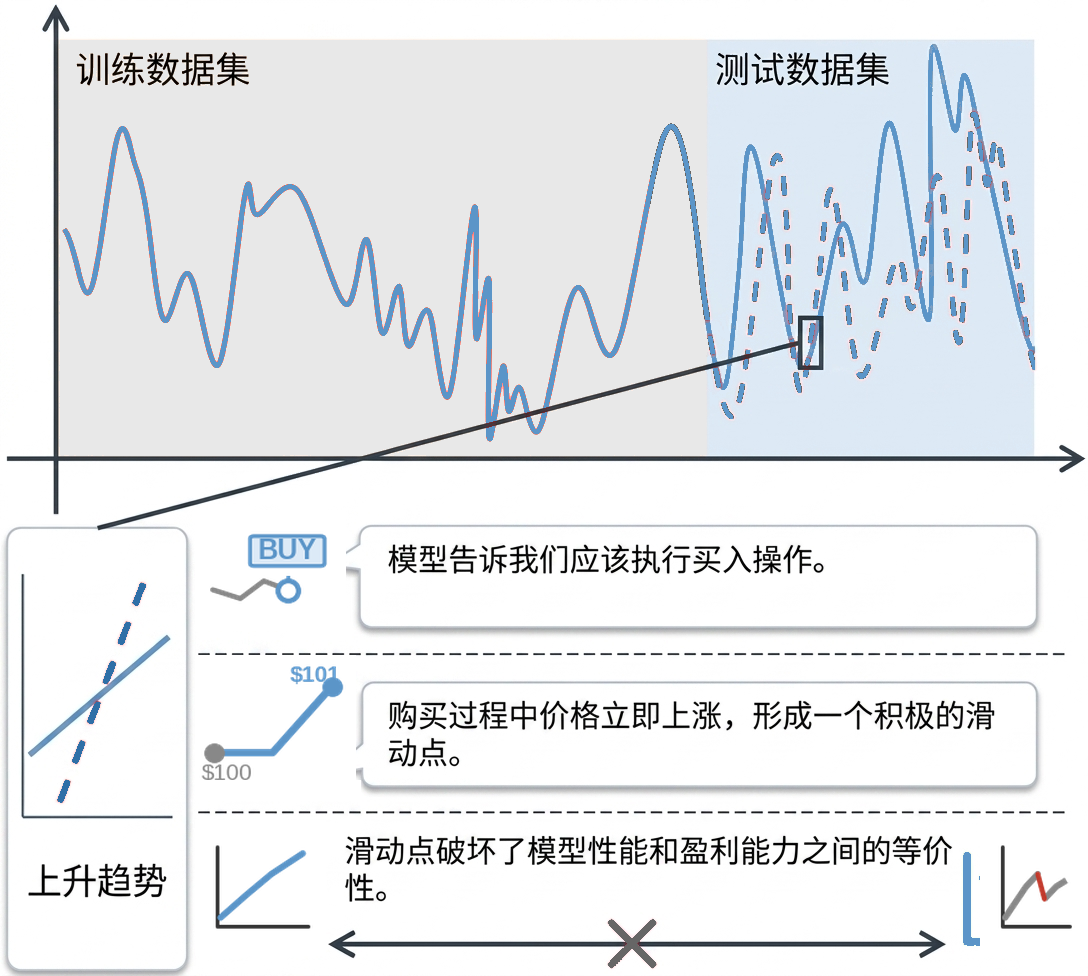
\includegraphics[width=\linewidth]{figures/chap6/图5.1改.png}
\caption{下单执行流程}
\label{fig:intro_new}
\end{figure}

图\ref{fig:intro_new}展示了从候选生成、孪生校验到最终下单执行的总体流程。该流程表明，本章方法并不替代前述模块，而是作为执行前的校验环节，对上游输出进行独立校验与风险过滤。

\begin{figure}[htbp]
    \centering 
    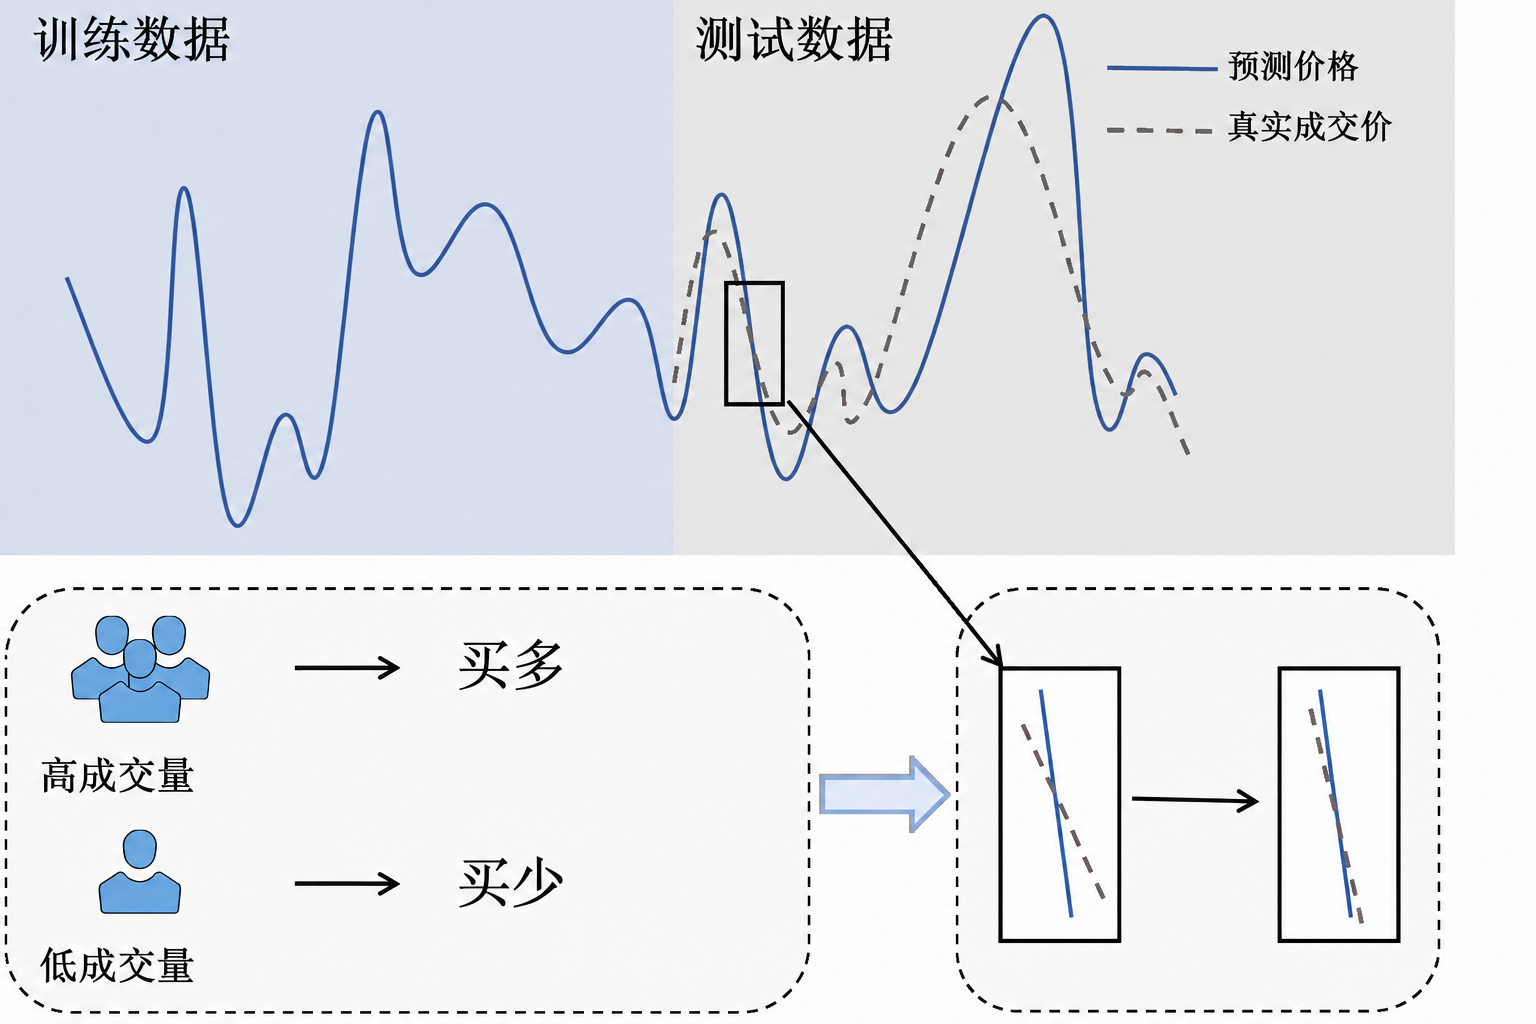
\includegraphics[width=0.8\textwidth]{figures/chap6/图5.2改.png} 
    \caption{孪生对抗自体再生方法在交易执行优化中的任务定位}
    \label{fig:vwap_task_new}
\end{figure}

图\ref{fig:vwap_task_new}给出了本章方法在多智能体对抗体系中的任务位置。其重点不在于追求单次预测最优，而在于判断系统能否在高噪声、厚尾与分布迁移环境中维持相对稳定的执行状态。

在此基础上，本章引入并系统性研究基于该机制减少滑点的方法（基于自体再生机制的成交量加权平均价格执行方法）。其基本思想是：以两个具有独立判别边界的成对子系统，对通过赛马场竞争机制选出的候选执行信号进行一致性认证；当任一子系统的模型偏离累计达到预设阈值时，触发替换与再平衡程序。这样，系统不再依赖单一判别器的一次性判断，而是在“双轨校验”中保留足够的容错空间。

\begin{figure}[htbp]
    \centering
    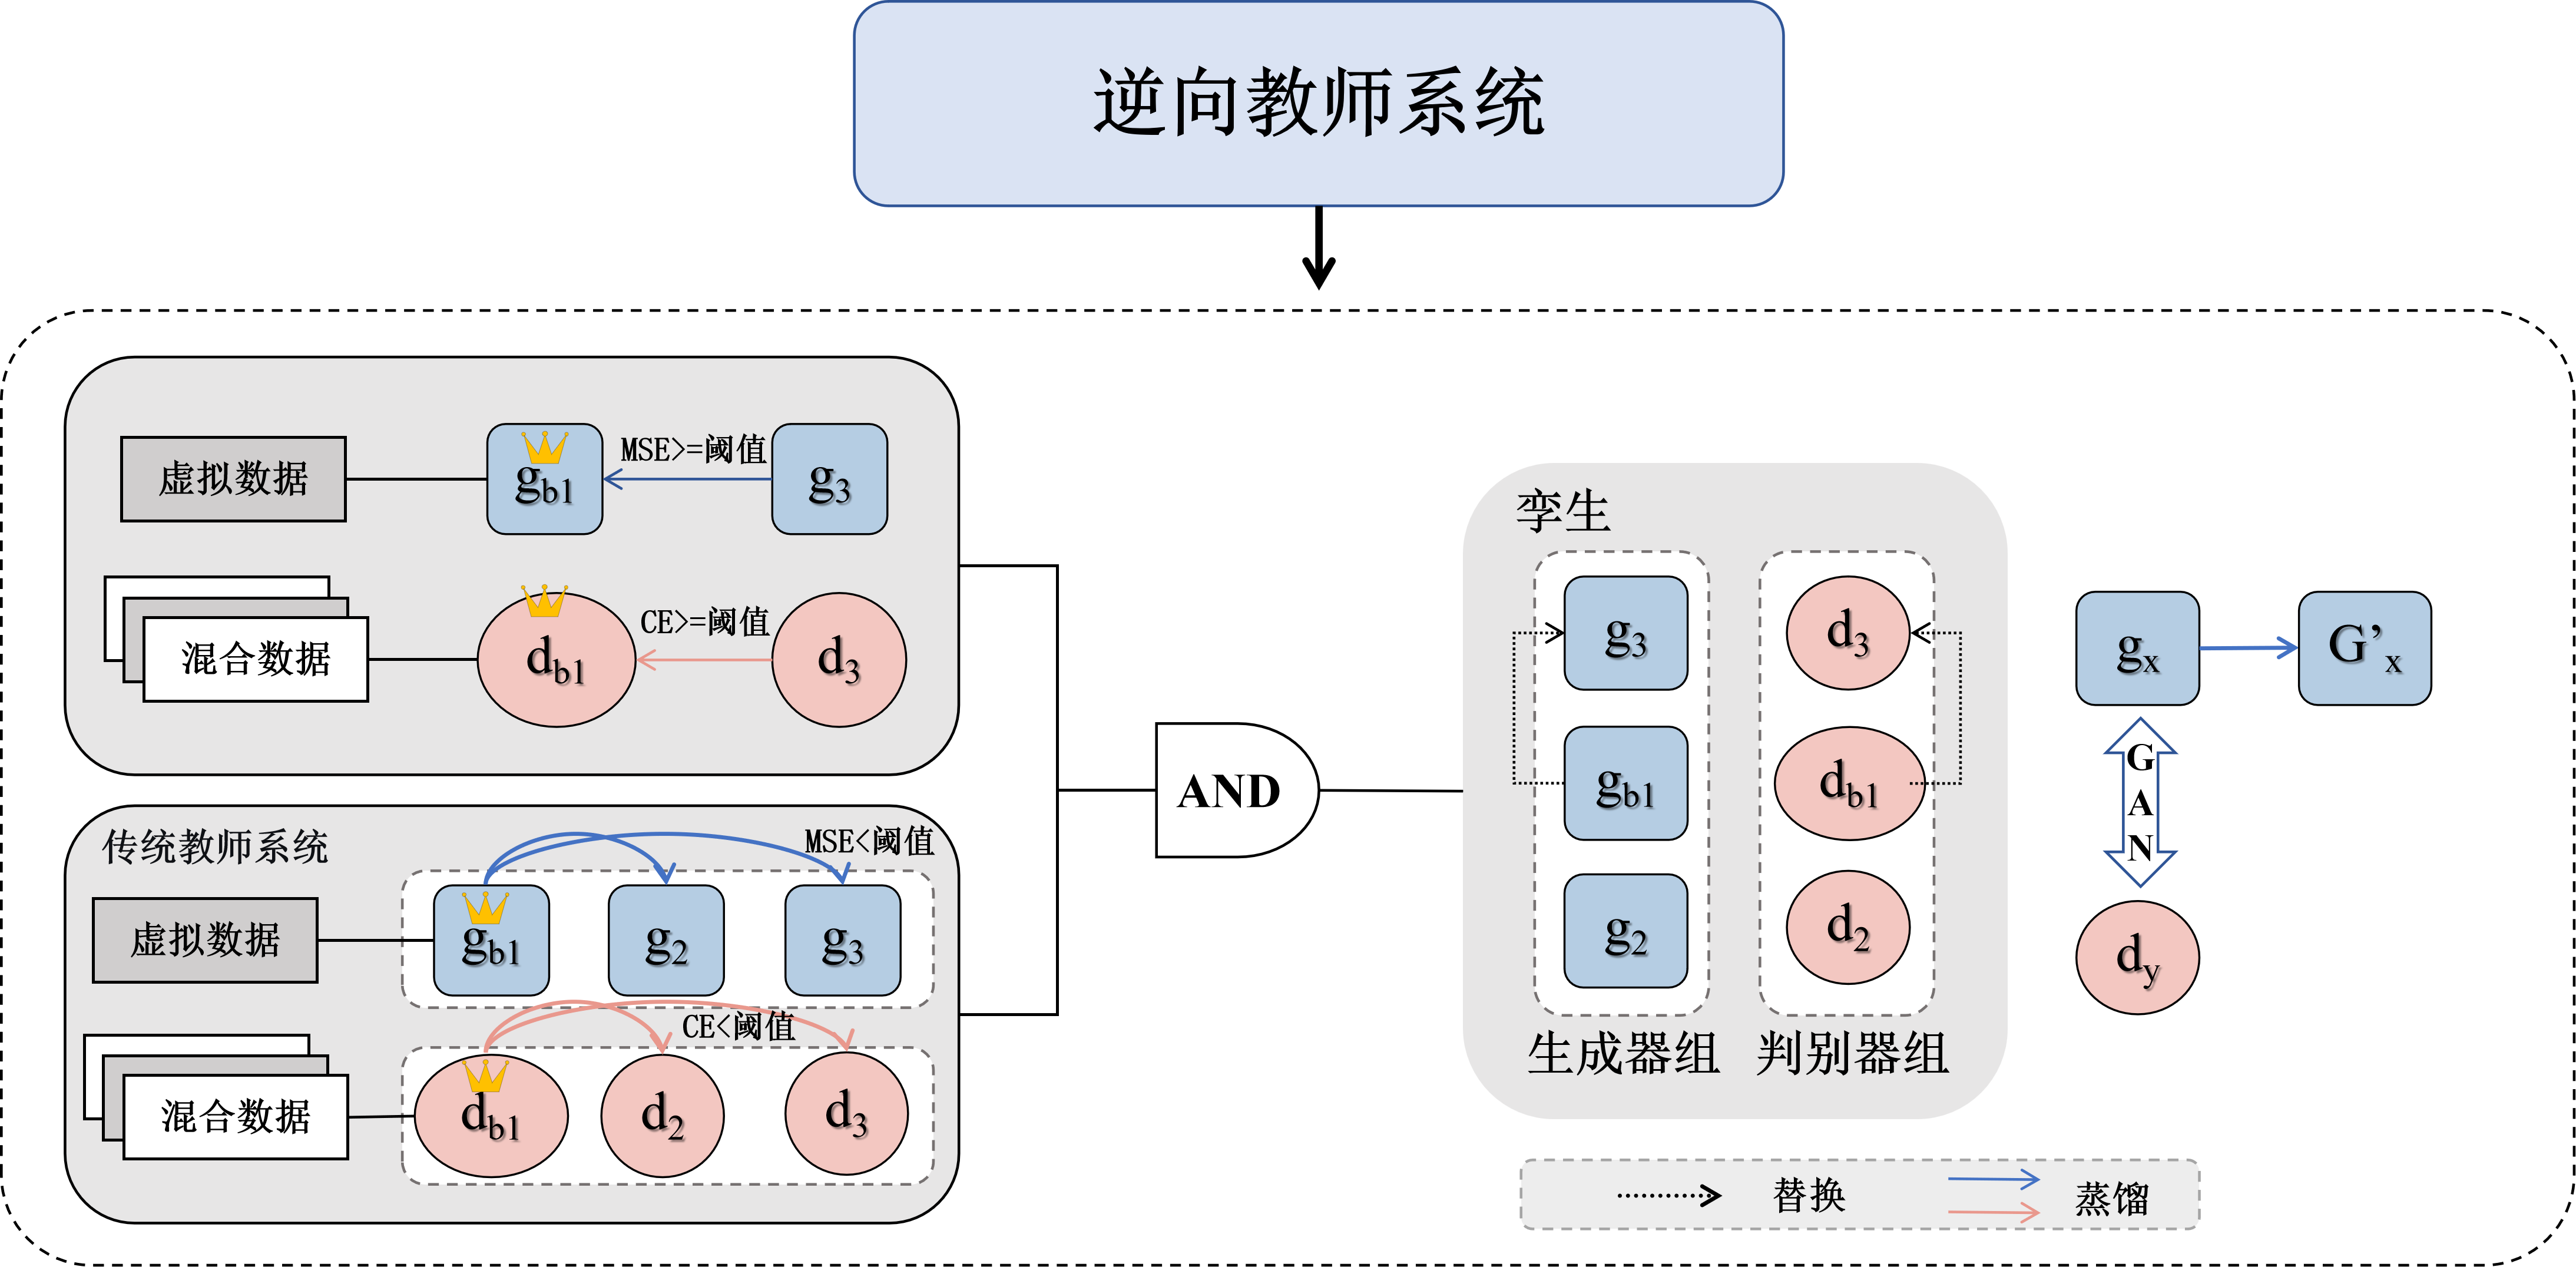
\includegraphics[width=0.8\textwidth]{figures/chap6/孪生对称.png}
    \caption{孪生对抗训练流程示意图}
    \label{fig:VWAP-workflow-new}
\end{figure}

图\ref{fig:VWAP-workflow-new}展示了孪生对抗训练流程。与传统单判别器结构相比，该流程通过复制优胜个体、为其建立独立对偶、并在后续训练中使其重新分化，使系统在保留高质量参数起点的同时避免完全同质化。这种“复制—配对—分化”逻辑，本质上是一种带有恢复能力的对抗冗余设计。

合作式多智能体学习研究指出，多主体系统若缺少明确的分工和反馈机制，容易出现学习效率下降或策略趋同的问题\cite{panait2005cooperative}。对本章而言，这一问题不能简单理解为模型数量不足，而应理解为复制后的候选主体能否形成可验证的功能差异。若孪生体在相同输入下持续给出趋同判断，复制过程只会增加冗余计算，难以形成对异常成交路径的有效校验。因此，后续自体再生机制需要在继承有效参数的同时，保留主体之间的差异化分工。

在金融投资任务中，多智能体组合管理系统也体现出通过分工学习不同资产或策略视角的价值\cite{lee2020maps}。这一思路映射到交易执行层，意味着孪生体不应只是重复给出同一执行判断，而应在相同订单约束下保留不同的风险过滤边界，用于比较候选信号是否会放大滑点、集中下单或触发异常成交路径。对做市任务的强化学习研究则表明，交易主体需要在收益、库存风险与成交概率之间持续权衡，这与本章执行层的风险过滤逻辑具有一致性\cite{spooner2018market}。因此，该机制中的复制并非简单克隆，而是在保留有效参数的同时重新建立差异化校验路径。

\subsection{跨组修复流程与崩溃抑制机制}

自体再生方法的设计动机，集中体现在对模型退化的可测量化处理上。尽管上游多智能体框架已能提升候选信号多样性与知识共享能力，执行层仍可能面临三类风险：生成器预测严重失真、判别器失效导致错误放行，以及模型组内同步退化并形成局部最优。为此，本章将“异常偏离”显式定义为可统计、可触发、可再平衡的数学对象。跨组修复流程的作用，是在局部模型组发生偏离时避免异常执行信号继续进入订单拆分与真实下单路径。与简单删除异常模型不同，本章将修复过程设计为受约束的再平衡过程：只有当偏离统计持续超过阈值，且其他模型组仍保持相对稳定时，系统才触发参数镜像或跨组替换；替换完成后，还需要通过短程对抗微调恢复新成员与原有群组之间的差异化边界。这样可以避免修复动作本身造成新的模型同质化或级联崩溃。对交易执行优化而言，模型崩溃并不只是训练过程中的技术问题，而会表现为错误成交量分布、异常订单切片或过度集中下单。跨组修复流程通过偏离统计与参数镜像机制，将这些潜在执行偏差前置到模型内部识别，从而降低异常信号直接转化为滑点和冲击成本的概率。

强化学习基础研究表明，序列决策问题通常通过状态、动作和奖励之间的反馈关系优化长期目标\cite{Mnih2015HumanlevelCT}。在交易执行任务中，这一思想可以进一步转化为对订单切片、成交概率和执行成本之间关系的动态优化；早期强化学习最优执行研究已经将交易执行明确表述为可通过市场反馈学习的决策问题\cite{nevmyvaka2006reinforcement_acm}。因此，本章将偏离统计量写入触发规则，是为了让执行风险在模型内部形成可追踪的反馈信号。

首先，对生成器或判别器引入偏离统计量。设每个成员的性能以均方误差或交叉熵表征，则生成器 $G_i$ 在时间步 $t$ 相对于当前最优生成器 $G_{\mathrm{best}}$ 的偏离度记为：
\begin{equation}
\Delta_i^{(t)} = \mathcal{L}(G_i, G_{\mathrm{best}}).
\label{eq:delta_stat_new}
\end{equation}
在训练过程中，若偏离度超过阈值 $\epsilon$，则对该成员累计一次超阈值计数：
\begin{equation}
N_i = \sum_{t=1}^{N} \mathbf{1}\left[ \Delta_i^{(t)} > \epsilon \right].
\label{eq:deviation_count_new}
\end{equation}
相应地，在更细粒度的实现中，生成器与判别器分别采用以下距离统计：
\begin{equation}
\delta_i^{(t)} = \mathrm{MSE}\left( G_i^{(t)}(x)_{:, -1, \text{close}},\; G_{\mathrm{best}}^{(t)}(x)_{:, -1, \text{close}} \right),
\end{equation}
\begin{equation}
\phi_j^{(t)} = \mathrm{MSE}\left( \mathrm{Feat}\left( D_j^{(t)}(G_i(x))\right),\; \mathrm{Feat}\left( D_{\mathrm{best}}^{(t)}(G_i(x))\right) \right).
\end{equation}
这意味着，系统不再依赖某一时刻的单次误差快照，而是通过跨 epoch 的慢变量统计识别“持续性偏离”。
当累计偏离达到阈值时，系统触发纠偏机制。其触发条件包含两层约束：其一，目标成员的超阈值次数达到设定阈值；其二，除目标组外至少存在另一组训练状态正常，防止系统从已退化群体中复制错误能力。满足条件后，对弱生成器或弱判别器执行深拷贝替换：
\[
G_i \gets \text{DeepCopy}(G_{\mathrm{best}}), \qquad
D_j \gets \text{DeepCopy}(D_{\mathrm{best}}).
\]
随后，同步重建优化器并进行短程对抗微调，以恢复竞争关系并重新形成差异化边界。
这种设计的关键价值在于，它将部分执行风险转化为训练阶段可追踪、推理阶段可触发的目标函数体系。模型是否出现异常、偏离是否持续、自体再生条件是否满足，均通过阈值、累计计数与跨组约束进行形式化表达。基于近端策略优化的端到端执行框架说明，执行策略可以直接围绕交易成本目标进行训练，而非只追求预测误差最小化\cite{lin2021ppo}。进一步的双层强化学习最优执行研究也提示，执行决策可被拆解为宏观调度与微观下单两个层面，使风险控制更加细粒度\cite{KIM2024124263}。因此，该机制并不只是附加的预测模块，而是将执行安全性纳入模型运行规则之中。

\subsection{滑点风险建模与执行层修复目标}

为刻画自体再生方法在执行层的作用，本节将候选信号生成、偏离识别、参数替换与短程对抗微调统一纳入交易执行优化流程。整体流程包括三步：第一，利用多智能体训练体系为孪生对抗自体再生提供候选池与偏离统计；第二，根据累计偏离和跨组约束识别弱模型并完成替换；第三，在替换后进行一轮对抗微调，使复制得到的参数重新进入可分化的博弈状态。算法交易研究指出，执行系统需要把预测信号、风险约束和交易规则组织成可复现的流程，而不能只停留在单个模型输出层面\cite{kearns2007algorithmic}。在数据驱动策略生成研究中，利用专家信息或敏感交易数据生成策略也需要额外的隐私与稳健性约束，也意味着候选信号进入执行前应经过独立校验\cite{chen2022generating}。从交易执行优化角度看，滑点风险在本章中不再被视为回测结果中的事后指标，而是被前置为执行层需要主动约束的优化目标。候选成交量分布、订单切片路径和孪生校验结果共同决定了执行系统是否继续沿当前路径下单；当模型偏离、流动性错配或成本扩散风险上升时，系统通过自体再生方法降低异常信号进入最终下单环节的概率。由此，成交量加权平均价格执行目标从“尽量贴近平均成交量曲线”扩展为“在可控成本与风险下稳定完成订单执行”。

为便于后续刻画执行层修复目标，本文将成交量加权平均价格、执行量约束、实际成交均价和滑点损失统一写为如下形式。设总执行时间窗口为 $T$，将其等分为 $N$ 个时间步，交易者需要完成总交易量为 $Q_{\mathrm{total}}$ 的指令。市场基准成交量加权平均价格定义为：
\begin{equation}
P_{\mathrm{VWAP}}=
\frac{\sum_{t=1}^{N} P_t^{\mathrm{mkt}} \cdot V_t^{\mathrm{mkt}}}{\sum_{t=1}^{N} V_t^{\mathrm{mkt}}}.
\label{eq:VWAP_definition_new}
\end{equation}
策略在每一时间步决定执行量 $q_t$，满足
\begin{equation}
\sum_{t=1}^{N} q_t = Q_{\mathrm{total}}, \qquad q_t \ge 0.
\label{eq:inventory_constraint_new}
\end{equation}
实际执行均价为：
\begin{equation}
\bar{P}_{\mathrm{exec}}=
\frac{\sum_{t=1}^{N} P_t^{\mathrm{exec}} \cdot q_t}{Q_{\mathrm{total}}},
\label{eq:exec_price_new}
\end{equation}
于是，以买单为例的滑点损失可写为：
\begin{equation}
\mathcal{L}_{\mathrm{slippage}}=
\left(\bar{P}_{\mathrm{exec}}-P_{\mathrm{VWAP}}\right)\cdot Q_{\mathrm{total}}.
\label{eq:slippage_loss_new}
\end{equation}
理想情况下，最优执行量分布应与市场成交量分布一致，即
\begin{equation}
\frac{q_t}{Q_{\mathrm{total}}}=
\frac{V_t^{\mathrm{mkt}}}{\sum_{k=1}^{N} V_k^{\mathrm{mkt}}}.
\label{eq:oracle_policy_new}
\end{equation}
上述公式说明，执行层优化不仅需要预测成交量密度，还需要使订单切片路径与市场流动性状态相匹配。

\begin{algorithm}[!htbp]
\caption{孪生对抗自体再生驱动的交易执行优化流程}
\label{alg:mgca_highdim_new}
\begin{algorithmic}[0]
\Require 期货品种列表 $\mathcal{A}$，任务类型集合 $\mathcal{T} = \{\text{regression}, \text{classification}, \text{investment}\}$，创新点开关 $\text{Enable}_{\text{GCA}}, \text{Enable}_{\text{RT}}, \text{Enable}_{\text{S2T}}, \text{Enable}_{\text{Twin}}$，训练集 $\mathcal{D}_{\text{train}}$，验证集 $\mathcal{D}_{\text{val}}$
\Ensure 各品种-任务组合的预测结果 $\mathcal{R}$，回测指标 $\mathcal{M}$
\State \textbf{/* 外层循环：遍历品种与任务 */}
\For{每种资产 $a \in \mathcal{A}$}
    \For{每种任务 $t \in \mathcal{T}$}
        \State 加载品种 $a$ 的开盘价、最高价、最低价、收盘价与成交量序列 $X_a$，归一化处理
        \State $Z_a \leftarrow \text{VAE\_Encode}(X_a)$
        \State 初始化生成器组 $\mathcal{G} = \{G_i\}$ 和判别器组 $\mathcal{D} = \{D_j\}$
        \If{$\text{Enable}_{\text{GCA}} = 1$}
            \State 执行组内交叉对抗 + 组间蒸馏
        \EndIf
        \If{$\text{Enable}_{\text{RT}} = 1$}
            \State 执行赛马场新学生竞争机制
        \EndIf
        \If{$\text{Enable}_{\text{S2T}} = 1$}
            \State 执行逆向师生蒸馏机制
        \EndIf
        \If{$\text{Enable}_{\text{Twin}} = 1$}
            \State 执行孪生对抗自体再生
        \EndIf
        \State $\hat{Y} \leftarrow G^{\star}(Z_a)$
        \State $\mathcal{R}_{a,t} \leftarrow \{\hat{Y}, Y_a\}$
    \EndFor
\EndFor
\State \Return $\mathcal{R}, \mathcal{M} \leftarrow \text{Backtest}(\mathcal{R})$
\end{algorithmic}
\end{algorithm}

算法\ref{alg:mgca_highdim_new}说明了孪生对抗自体再生方法的输入来源与执行位置：前序机制为本章提供候选池与偏离统计，本章则在执行层完成信号校验、弱模型替换和短程再平衡。随后，系统进入孪生对抗自体再生与替换阶段。

\begin{algorithm}[!htbp]
    \caption{孪生对抗自体再生与弱模型替换（第一部分）}
    \label{alg:twin_detection_new}
    \begin{algorithmic}[0]
    \Require 训练完成的生成器组 $\mathcal{G}_{\text{groups}}$、判别器组 $\mathcal{D}_{\text{groups}}$、孪生参数 $\epsilon_{\mathrm{gen}},\epsilon_{\mathrm{disc}},\text{twin\_nums\_threshold}$、验证集 $\mathcal{D}_{\mathrm{val}}$
    \Ensure 待微调的生成器 $G_{\mathrm{sel}}$、判别器 $D_{\mathrm{sel}}$
    \State \textbf{第一步：各组内评估并定位最优成员}
    \For{每组生成器 $\mathcal{G}^{(g)} \in \mathcal{G}_{\text{groups}}$}
        \State 计算组内每个生成器的验证集均方误差，找出均方误差最小的 $G_{\mathrm{best}}^{(g)}$
    \EndFor
    \For{每组判别器 $\mathcal{D}^{(d)} \in \mathcal{D}_{\text{groups}}$}
        \State 计算组内每个判别器的验证集二元交叉熵，找出二元交叉熵最小的 $D_{\mathrm{best}}^{(d)}$
    \EndFor
    \State \textbf{第二步：逐组检测弱生成器并替换}
    \For{每组生成器 $\mathcal{G}^{(g)}$}
        \State 识别满足阈值条件的弱生成器集合 $\mathcal{W}_{\mathrm{gen}}$
        \State 若除 $g$ 组外至少有一组训练状态正常，则对 $\mathcal{W}_{\mathrm{gen}}$ 执行深拷贝替换
    \EndFor
    \State \textbf{第三步：逐组检测弱判别器并替换}
    \For{每组判别器 $\mathcal{D}^{(d)}$}
        \State 识别满足阈值条件的弱判别器集合 $\mathcal{W}_{\mathrm{disc}}$
        \State 若跨组约束满足，则对 $\mathcal{W}_{\mathrm{disc}}$ 执行深拷贝替换
    \EndFor
    \State 任选生成器 $G_{\mathrm{sel}}$ 和判别器 $D_{\mathrm{sel}}$
    \State \Return $G_{\mathrm{sel}},\; D_{\mathrm{sel}}$
    \end{algorithmic}
\end{algorithm}

\begin{algorithm}[!htbp]
    \caption{孪生对抗生成对抗网络微调（第二部分）}
    \label{alg:twin_finetune_new}
    \begin{algorithmic}[0]
    \Require 待微调的生成器 $G_{\mathrm{sel}}$、判别器 $D_{\mathrm{sel}}$、训练集 $\mathcal{D}_{\mathrm{train}}$
    \Ensure 稳定恢复后的最优生成器 $\mathcal{G}_{\mathrm{best}}$、判别器 $\mathcal{D}_{\mathrm{best}}$
    \State \textbf{第四步：生成对抗网络微调以恢复对抗平衡}
    \State 在训练集 $\mathcal{D}_{\mathrm{train}}$ 上执行一个 epoch 的对抗训练
    \State 判别器最小化 $\mathcal{L}_D = \frac{1}{2} [ \mathrm{BCE}(D_{\mathrm{sel}}(x_{\mathrm{real}}), 1) + \mathrm{BCE}(D_{\mathrm{sel}}(G_{\mathrm{sel}}(x)), 0) ]$
    \State 生成器最小化 $\mathcal{L}_G = \mathcal{L}_G^{\mathrm{adv}} + \mathcal{L}_G^{\mathrm{recon}}$
    \State $\mathcal{G}_{\mathrm{best}} \gets G_{\mathrm{sel}}$，$\mathcal{D}_{\mathrm{best}} \gets D_{\mathrm{sel}}$
    \State \Return $\mathcal{G}_{\mathrm{best}},\; \mathcal{D}_{\mathrm{best}}$
    \end{algorithmic}
\end{algorithm}

下面对算法\ref{alg:mgca_highdim_new}、\ref{alg:twin_detection_new}、\ref{alg:twin_finetune_new}进行复杂度分析。

\textbf{时间复杂度：} 设资产数量为 $|\mathcal{A}|$，任务类型数 $|\mathcal{T}|=3$，生成器与判别器数量分别为 $N_G$、$N_D$，批大小为 $B$，时间窗口长度为 $W$，隐藏层维度为 $d$。外层循环总实验次数为 $|\mathcal{A}| \cdot |\mathcal{T}|$，各实验独立运行。单次实验中，GCA阶段复杂度为 $O(N_G \cdot B \cdot W^2 \cdot d)$，赛马场竞争机制阶段引入学生模型培养与末位淘汰，附加复杂度 $O(N_G \cdot |\mathcal{D}_{\text{val}}| \cdot W^2 \cdot d)$。逆向师生蒸馏阶段增加蒸馏计算，复杂度为 $O((N_G+N_D) \cdot d)$。孪生检测算法中，各组评估复杂度为 $O((N_G+N_D) \cdot |\mathcal{D}_{\text{val}}| \cdot W^2 \cdot d)$，弱模型识别与深拷贝替换复杂度为 $O(N_G \cdot |\theta_G| + N_D \cdot |\theta_D|)$。孪生微调算法执行单epoch对抗训练，复杂度为 $O((N_G+N_D) \cdot B \cdot W^2 \cdot d)$。总体时间复杂度约为 $O(|\mathcal{A}| \cdot |\mathcal{T}| \cdot (N_G+N_D) \cdot (B + |\mathcal{D}_{\text{val}}|) \cdot W^2 \cdot d)$。

\textbf{空间复杂度：} 模型参数存储为 $O(N_G \cdot |\theta_G| + N_D \cdot |\theta_D|)$，Adam优化器状态为 $O(2(N_G \cdot |\theta_G| + N_D \cdot |\theta_D|))$。激活值存储为 $O((N_G+N_D) \cdot B \cdot W \cdot d)$。验证集特征存储为 $O(|\mathcal{D}_{\text{val}}| \cdot W \cdot d)$。深拷贝操作临时需额外 $O(|\theta_G| + |\theta_D|)$ 空间。

上述算法保留了原始方法论中的关键细节，但其逻辑可以概括为：在逆向师生蒸馏训练阶段同步积累偏离证据，在孪生对抗自体再生阶段执行跨组约束下的弱模型替换，再以短程生成对抗网络微调恢复孪生系统的对抗张力。至此，“复制—配对—分化”的自体再生程序便完成基本流程。该流程还需要面对一个实践问题：市场状态并非由模型单方面决定，而会随着订单提交、成交反馈和对手方行为持续变化。交易图神经网络相关研究说明，资产与交易主体之间的关系结构会影响交易信号的传播方式，执行模型因此需要关注跨资产与跨状态的联动关系\cite{wu2025tgnn}。

\section{实验}

本章实验围绕交易执行优化任务展开，重点检验孪生对抗自体再生方法能否在不同品种、不同波动状态和不同成交量结构下降低执行偏差与滑点风险。实验评价不以单一预测误差为唯一标准，而是结合成本节省、收益率、胜率、回撤控制和下行风险等执行层指标，判断模型能否将上游信号稳定转化为可落地的下单路径。为对应前文提出的问题，实验部分重点观察三类关系：成交量预测是否能够支持订单时间分布生成，动态执行路径是否能够降低相对成交量加权平均价格的滑点，孪生校验与自体再生是否能够在模型退化时维持执行稳定性。

\subsection{实验数据集}

本章数据集的设置服务于交易执行优化任务，重点考察模型在真实高频期货数据中的成交量分布预测、订单拆分路径生成与成交量加权平均价格执行表现。实验数据覆盖中国期货市场 19 个代表性品种，横跨贵金属、有色金属、金融期货、农产品、黑色金属和能源化工六大类，共包含 279 个时间段与 697,500 个数据点。每个时间段由连续 2,500 个 1 分钟数据点构成，并进一步切分为训练集、验证集与测试集，用于模型训练、调参与成交量加权平均价格执行模拟。数据时间跨度为 2020 年 1 月至 2025 年 6 月，覆盖牛市、熊市与震荡市等不同阶段，因此能够较充分地检验该方法在多种市场环境下的鲁棒性。高频金融时间序列通常存在尺度差异和双线性结构，若标准化处理不当，模型可能把交易制度或品种尺度差异误当成有效信号\cite{tran2021data}。对于本章的执行优化任务而言，标准化处理还需要避免抹平分钟级成交量分布中的局部峰谷，因为这些短时集中成交往往会影响订单拆分节奏和成交量加权平均价格偏离。换言之，数据预处理既要消除跨品种尺度差异，也要保留能够反映流动性聚集和短期冲击的动态结构。此外，订单流在高频场景中常表现出自激发特征，Hawkes 过程在金融中的应用研究为理解订单簿事件聚集提供了重要工具\cite{2015Hawkes}。


\begin{table}[H]
\centering
\caption{数据集概览}
\label{tab:dataset_overview_new}
\begingroup
\small
\setlength{\tabcolsep}{3.5pt}
\renewcommand{\arraystretch}{0.86}
\resizebox{0.98\textwidth}{!}{%
\begin{tabular}{lllc@{\hspace{1.2em}}lllc}
\toprule
\textbf{类别} & \textbf{品种} & \textbf{品种代码} & \textbf{时间段数} & \textbf{类别} & \textbf{品种} & \textbf{品种代码} & \textbf{时间段数} \\
\midrule
\multirow{2}{*}{贵金属}   & 黄金       & au & 22 & \multirow{5}{*}{农产品}   & 玉米       & c  & 14 \\
                         & 白银       & ag & 22 &                          & 豆粕       & m  & 14 \\
\cmidrule(lr){1-4}
\multirow{2}{*}{有色金属} & 铜         & cu & 18 &                          & 豆油       & y  & 14 \\
                         & 镍         & ni & 18 &                          & 棉花       & CF & 14 \\
                         &            &    &    &                          & 苹果       & AP & 9  \\
\midrule
\multirow{3}{*}{金融期货} & 沪深300股指 & IF & 16 & \multirow{5}{*}{能源化工} & 原油       & sc & 21 \\
                         & 上证50股指  & IH & 12 &                          & 液化石油气 & pg & 14 \\
                         & 10年期国债  & T  & 10 &                          & 对苯二甲酸 & TA & 14 \\
\cmidrule(lr){1-4}
\multirow{2}{*}{黑色金属} & 铁矿石     & i  & 14 &                          & 菜籽油     & OI & 14 \\
                         & 螺纹钢     & rb & 14 &                          & 尿素       & UR & 9  \\
\bottomrule
\end{tabular}%
}
\endgroup
\end{table}

表\ref{tab:dataset_overview_new}表明，各品种在波动率、流动性和市场驱动因素上具有明显异质性。贵金属流动性较高且受避险情绪影响明显；有色金属受全球周期影响更强，波动水平相对较高；金融期货覆盖了低波动国债与中高波动股指；农产品具有季节性和外部冲击特征；黑色金属更受产业周期与政策影响；能源化工则呈现高噪声和复杂供需博弈特征。正是这种跨品种、跨波动状态的数据结构，使得静态执行基准的局限性更容易暴露，也为检验该机制提供了真实场景。近年来，限价订单簿自注意力模型研究表明，盘口状态的时空依赖可以通过注意力结构进行刻画，这为高频执行中的分钟级状态识别提供了参考\cite{xiao2025lit}。对于本章任务而言，盘口状态识别并不是独立的价格预测目标，而是服务于成交量分布估计、流动性厚度判断和订单拆分节奏控制。若模型只捕捉局部价格或盘口变化，而不能同时识别这些变化在时间维度上的延续性与空间层级上的传导关系，执行路径仍可能在局部拥挤时段产生偏差。限价订单簿时空模型等时空自注意力模型方法进一步强调，订单簿预测需要同时处理时间动态与空间层级结构\cite{berti2025tlob}。

为进一步观察不同品种在预测误差、执行改善和胜率表现上的差异，图\ref{fig:fullmgcatwin19varietiesdataanalysis9_new}对 19 个品种的综合特征进行了汇总。

\begin{figure}[H]
\centering
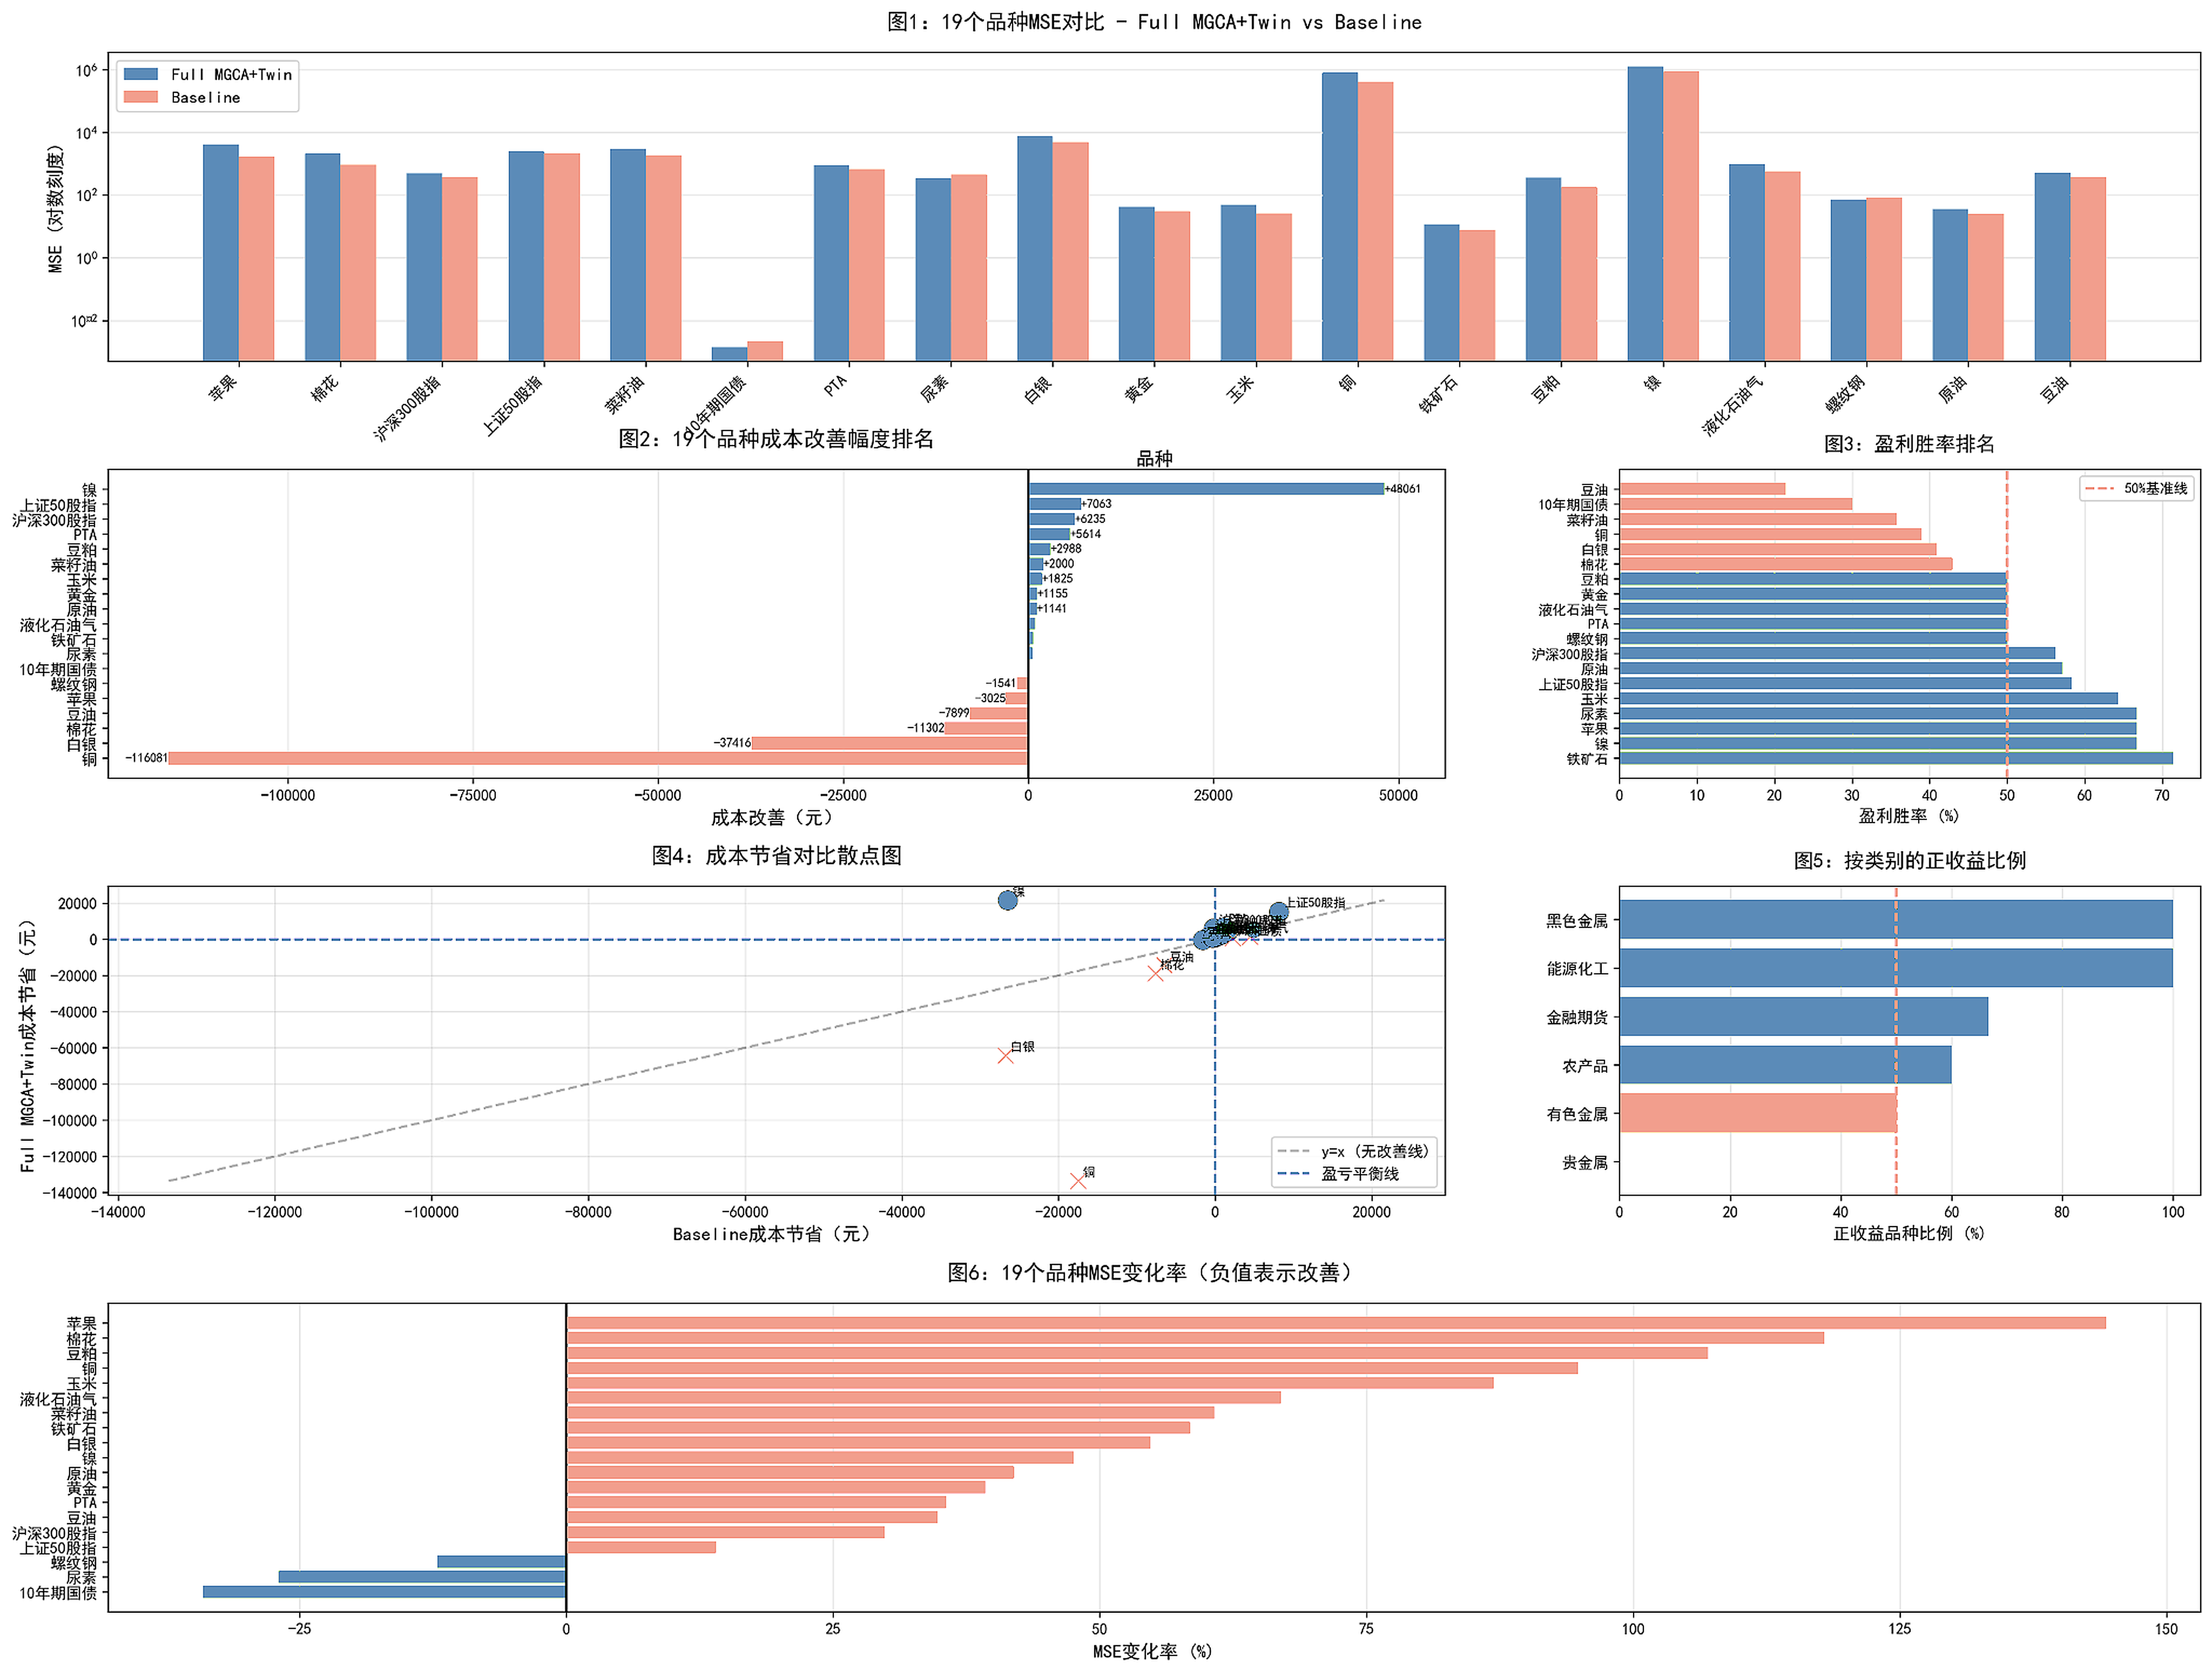
\includegraphics[width=0.95\textwidth]{figures/chap6/图5.4改.png}
\caption{孪生对抗框架在19个品种上的综合数据特征分析}
\label{fig:fullmgcatwin19varietiesdataanalysis9_new}
\end{figure}

图\ref{fig:fullmgcatwin19varietiesdataanalysis9_new}汇总了 19 个品种的均方误差分布、成本改善与盈利胜率等关键信息。结果显示，品种间预测难度与执行效果并不一致：有色金属类具有最高均方误差，但部分品种仍取得了较好的成本改善；铁矿石、镍、苹果和尿素等品种则在胜率上表现突出。这意味着，执行层优势并不简单来自拟合误差降低，而更依赖模型是否能够识别关键流动性结构并过滤异常信号。


在综合特征之外，图\ref{fig:volatilityverificationanalysis_new}进一步从波动率分层角度考察不同品种的市场状态差异。

\begin{figure}[H]
\centering
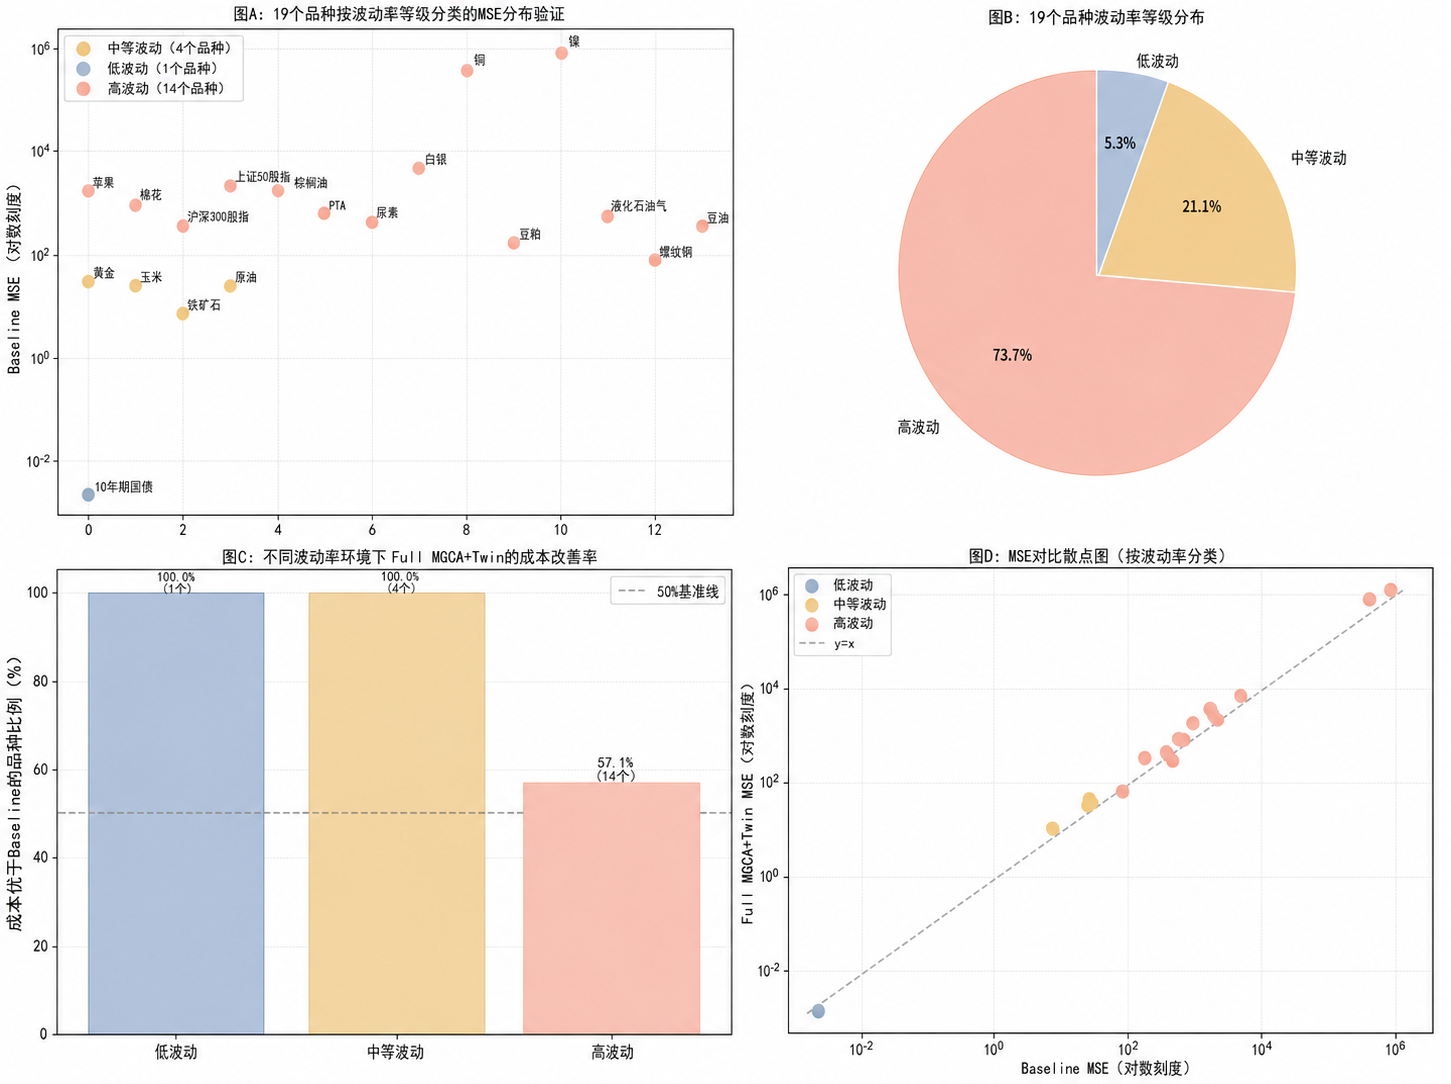
\includegraphics[width=0.85\textwidth]{figures/chap6/图5.5改}
\caption{孪生对抗框架在19个品种上的波动率分类验证与市场特征分析}
\label{fig:volatilityverificationanalysis_new}
\end{figure}

图\ref{fig:volatilityverificationanalysis_new}进一步给出了以基准模型均方误差为代理变量的波动率分层结果。低波动品种仅有 10 年期国债，中等波动品种包括铁矿石、原油、玉米和黄金，高波动品种占样本主体。在低波动和中等波动环境下，孪生对抗框架实现了 100\% 的成本改善率；即便在高波动环境中，仍有超过一半的品种获得正向改善。这表明，多生成器覆盖与孪生校验的组合，在中高波动、非平稳环境中尤其具有现实意义。

上述数据分布与波动率分层结果说明，本章实验不仅需要检验整体执行效果，还需要在不同波动状态和品种结构下考察方法的稳定性。基于此，下一节进一步说明实验设计与评价指标。

\subsection{实验设计}

本节围绕交易执行路径优化展开实验设计：在给定交易信号和执行窗口的条件下，考察不同模型如何生成下单路径，以及这些路径在滑点、成本节省和风险控制指标上的差异。实验设计包括三个层面：第一，基于高频期货数据生成成交量预测与候选执行路径；第二，将候选信号映射为 30 分钟成交量加权平均价格执行窗口内的动态下单比例；第三，通过成本节省、收益率、胜率、回撤控制和风险收益比等指标检验执行优化效果。

% 在完成候选成交量分布的生成与筛选后，调度器作为下游决策层，负责将通过认证的信号映射为可执行的下单路径\cite{bertsimas1998optimal,cartea2016closed,frei2015optimal,konishi2002optimal}。
在完成候选成交量分布的生成与筛选后，调度器作为下游决策层，负责将通过认证的信号映射为可执行的下单路径\cite{bertsimas1998optimal}。这一设置并不是将预测结果直接转化为一次性交易指令，而是先根据剩余订单量和执行时间窗口确定分段下单节奏，再检验不同模型输出能否改善成交量加权平均价格跟踪效果。最优执行问题的早期研究已从理论层面证明，在线性冲击假设下，最优策略具有封闭形式解，为后续动态调度器的设计提供了重要基础\cite{cartea2016closed}。

在随机控制框架下，Frei 与 Westray 进一步将成交量加权平均价格执行问题形式化为一类有限时间随机最优控制问题，其结论对非平稳成交量条件下的鲁棒执行具有重要参考价值\cite{frei2015optimal}。
与此同时，Konishi 从订单切片的角度出发，系统研究了如何在约束条件下实现对成交量加权平均价格基准的最优追踪，为本章调度器的分段设计提供了方法论依据\cite{konishi2002optimal}。
最优执行综述指出，现代执行模型需要在市场冲击、风险暴露、完成约束和成交量预测之间做联合权衡，而不是只优化单一成交均价\cite{gatheral2022optimal}。因此，本章实验并不只比较预测曲线是否更平滑，而是进一步检验预测结果能否形成稳定的分段下单节奏。
在日内市场中，最优下单路径会受到流动性峰谷和时间约束共同影响，静态曲线难以覆盖全部情形\cite{kath2020optimal}。这也是本文保留“预测阶段—兜底阶段”两段式安排的原因：前段依据预测成交量密度分配订单，后段在剩余时间不足或预测偏离时完成收尾。
基于长短期记忆网络的大额订单执行控制研究则表明，成交量和价格路径可以被纳入序列控制框架，为本章双阶段调度提供了方法参考\cite{papanicolaou2023optimal}。对于剩余订单量 $R_t$ 与预测成交量密度 $\hat{\mathbf{v}}=[\hat{v}_1,\dots,\hat{v}_N]$，执行器在预测阶段按照
\begin{equation}
q_t = R_t \cdot \frac{\hat{v}_t}{\sum_{k=t}^{N} \hat{v}_k}
\label{eq:dynamic_schedule_new}
\end{equation}
进行动态拆分；当进入收盘兜底阶段，则采用几何级数加速完成剩余订单：
\begin{equation}
q_t = R_t \cdot \frac{1-r}{1-r^{N-t+1}}, \qquad r\in(0,1).
\label{eq:closing_phase_new}
\end{equation}
其中，前者确保订单时间分布尽量贴近预测成交量分布，后者则在最后阶段通过加速执行保证完成率。两者结合，使得成交量加权平均价格调度既保留了对未来流动性的主动感知，又避免了因预测误差导致的未完成风险。

从执行流程看，30 分钟成交量加权平均价格窗口被划分为 30 个 1 分钟时间片。前 25 分钟属于“基于预测”阶段，执行器以未来成交量权重决定当前下单比例；后 5 分钟进入“收盘冲刺”阶段，以几何级数规则消化剩余头寸；若剩余量提前接近零，则进入“提前完成”状态。该设计将信号生成、实时分配与兜底收敛有机结合，使动态调度器能够在实际交易约束下稳定运行。成交量加权平均价格的最优执行研究表明，将成交量预测显式纳入下单路径能够提高对成交量加权平均价格基准的跟踪能力\cite{busseti2015volume}。因此，本章并不要求模型一次性给出完整订单序列，而是先预测短窗口内的成交量密度，再结合剩余订单量逐分钟更新下单比例。这样既利用了预测阶段对未来流动性的判断，也为后续兜底阶段保留了修正空间。分层深度强化学习用于成交量加权平均价格策略优化的研究也提示，执行任务可以拆成高层调度和低层执行两个子任务，从而降低单一策略直接学习完整路径的难度\cite{10336391}。

为保证后续结果可比，本章所有回测均以 10,000 单位统一下单量执行，并将每个 30 分钟窗口视作一个独立任务。每个窗口结束后，系统根据模型实现价格与基准成交量加权平均价格计算成本节省，再进一步换算为 时间段收益率、年化收益率、胜率、盈亏比、最大回撤、夏普比率、卡玛比率与索提诺比率等指标。由此，评估体系同时覆盖了拟合层指标和执行层指标，能够从拟合与执行两个层面评价策略的经济含义。

在回测框架与交易性能指标方面，本章的回测目标是量化孪生对抗框架在降低滑点、提升执行效率方面的经济价值。与单纯评价均方误差、平均绝对百分比误差的拟合分析不同，回测部分同时使用成本节省、收益率、胜率、盈亏比、最大回撤、夏普比率、卡玛比率、索提诺比率以及最大连胜连亏等指标，构成“拟合层—执行层”双重评价体系。

设每个成交量加权平均价格执行窗口的统一交易数量为 10,000 单位，投入资本定义为 $C_{\text{capital}} = Q \times \text{VWAP}_{\text{benchmark}}$。则单个窗口的收益率为
\begin{equation}
r_{\text{segment}} = \frac{\text{CostSaving}}{C_{\text{capital}}} \times 100\%.
\end{equation}
根据原始 1 分钟 K 线数据的统计结果，每日平均交易时间约为 372 分钟，对应 12.4 个 30 分钟窗口；结合每年 252 个交易日，可得年化倍数 3125。因此，年化收益率定义为 $\bar r_{\text{annual}} = \bar r_{\text{segment}} \times 3125$。其中，这里的“年化收益率”表示执行效率的年度等效表达，而不是账户复利增长。

在此框架下，成交量加权平均价格下单策略可概括为三阶段：其一，在前 25 分钟内依据预测成交量比例进行动态下单；其二，在最后 5 分钟采用几何级数规则加速完成剩余订单；其三，若剩余量已接近零，则提前停止下单。该策略与孪生校验机制结合后，使系统能够在预测和兜底之间取得平衡，避免因单一规则导致的过度交易或未完成执行。机器学习交易系统的相关思路表明，执行评价需要回到可交易规则与真实成本，而不能只依据离线预测结果判断模型优劣。

\subsection{结果分析与讨论}

本节围绕交易执行优化目标，对实验结果进行分组分析。为避免将图表简单堆叠为结果清单，下文按照“拟合表现与成交量预测—收益与胜率—风险收益结构—跨品种成本改善”的顺序展开：首先利用代表性价格预测、误差分布、训练稳定性与成交量预测结果说明候选信号是否具备进入执行路径的基础；随后结合收益率、胜率和风险收益指标，检验孪生对抗自体再生方法是否能够降低滑点传导和执行退化风险；最后通过跨品种成本改善结果讨论其适用边界。

需要说明的是，本章不以单一预测误差作为唯一评价依据，而是关注候选信号能否在真实执行窗口中转化为更稳定的下单路径。价格预测图、成交量预测图和误差分布主要用于说明模型对局部结构的刻画能力；成本节省、收益率、胜率和风险收益指标则用于检验执行路径是否在实际交易评价中降低滑点和市场冲击。

在拟合性能与成交量预测结果方面，黄金期货是本章的代表性案例之一。该数据集包含 22 个时间段，总计 55,000 个数据点，具有相对稳定但并不简单的价格结构。下文先比较价格路径拟合效果，再从误差分布、训练稳定性和成交量预测三个角度检验该机制是否能够服务于成交量加权平均价格执行优化。

首先观察价格路径拟合结果。图\ref{fig:au9999exp0baselinepredictions_new}与图\ref{fig:au9999exp7twinpredictions_new}分别给出了基准模型和孪生对抗框架在同一黄金期货时间段上的预测表现。

\begin{figure}[!htbp]
\centering
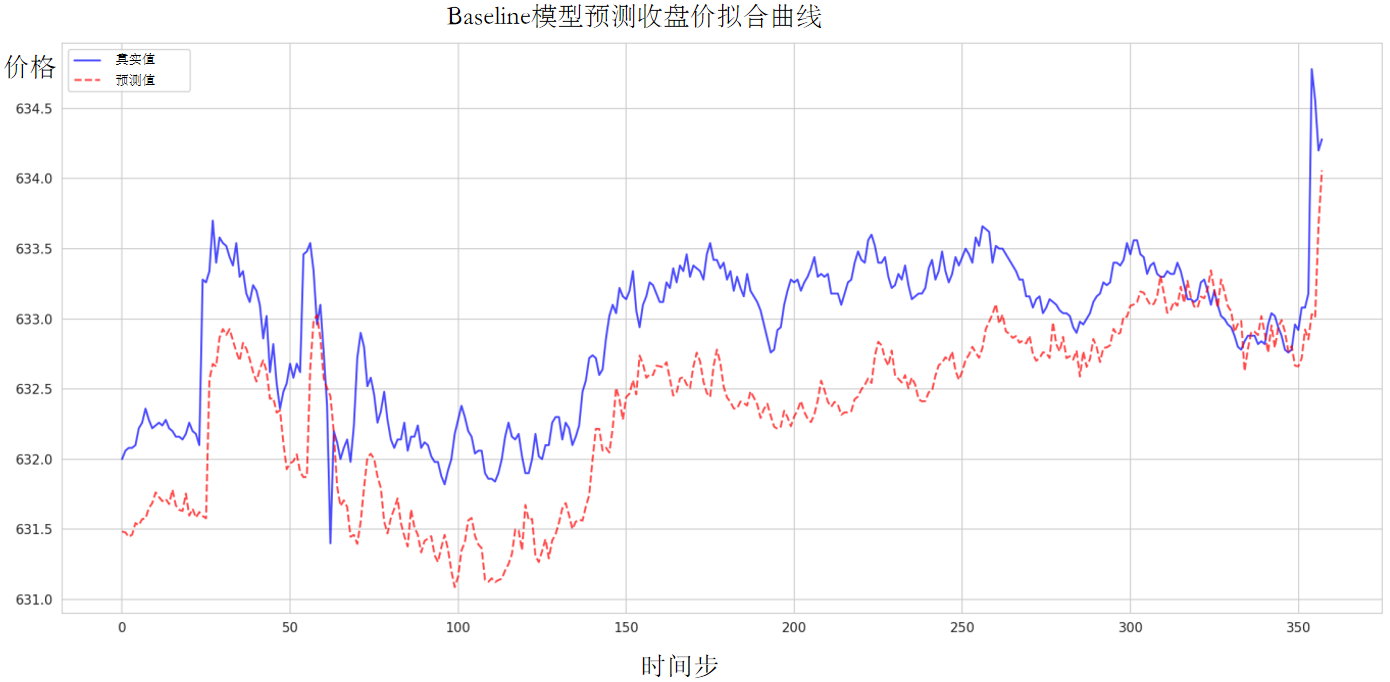
\includegraphics[width=0.80\textwidth]{figures/chap6/au_baselinepredictioncurve.png}
\caption{基准模型在黄金期货时间段002上的价格预测表现}
\label{fig:au9999exp0baselinepredictions_new}
\end{figure}

\begin{figure}[!htbp]
\centering
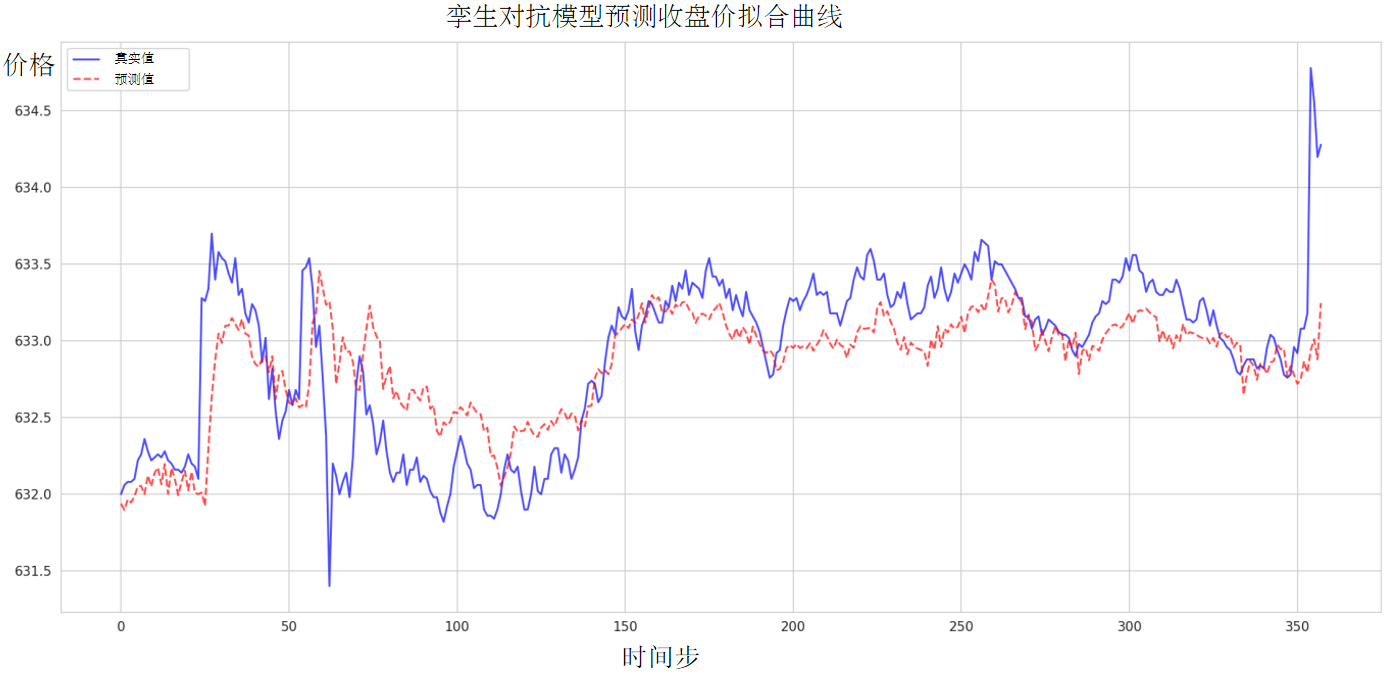
\includegraphics[width=0.80\textwidth]{figures/chap6/au_fullmgcatwinpredictioncurve.png}
\caption{孪生对抗框架在黄金期货时间段002上的价格预测表现}
\label{fig:au9999exp7twinpredictions_new}
\end{figure}

从两张价格预测图可以看出，在代表性时间段上，孪生对抗的价格预测曲线与真实价格的贴合度更高，平均绝对百分比误差由 0.0977 降至 0.0474，改善幅度为 51.51\%。这一改进并不意味着所有品种上均方误差都同步改善，但它证明了在关键局部结构上，该机制能够提供更稳定的方向捕捉能力，并在该时间段实现 2,218.80 元的成本改善。

进一步从误差分布角度观察模型稳定性。图\ref{fig:au9999exp7twinerroranaly_new}给出了孪生对抗框架在黄金期货上的误差分布结果。

\begin{figure}[!htbp]
\centering
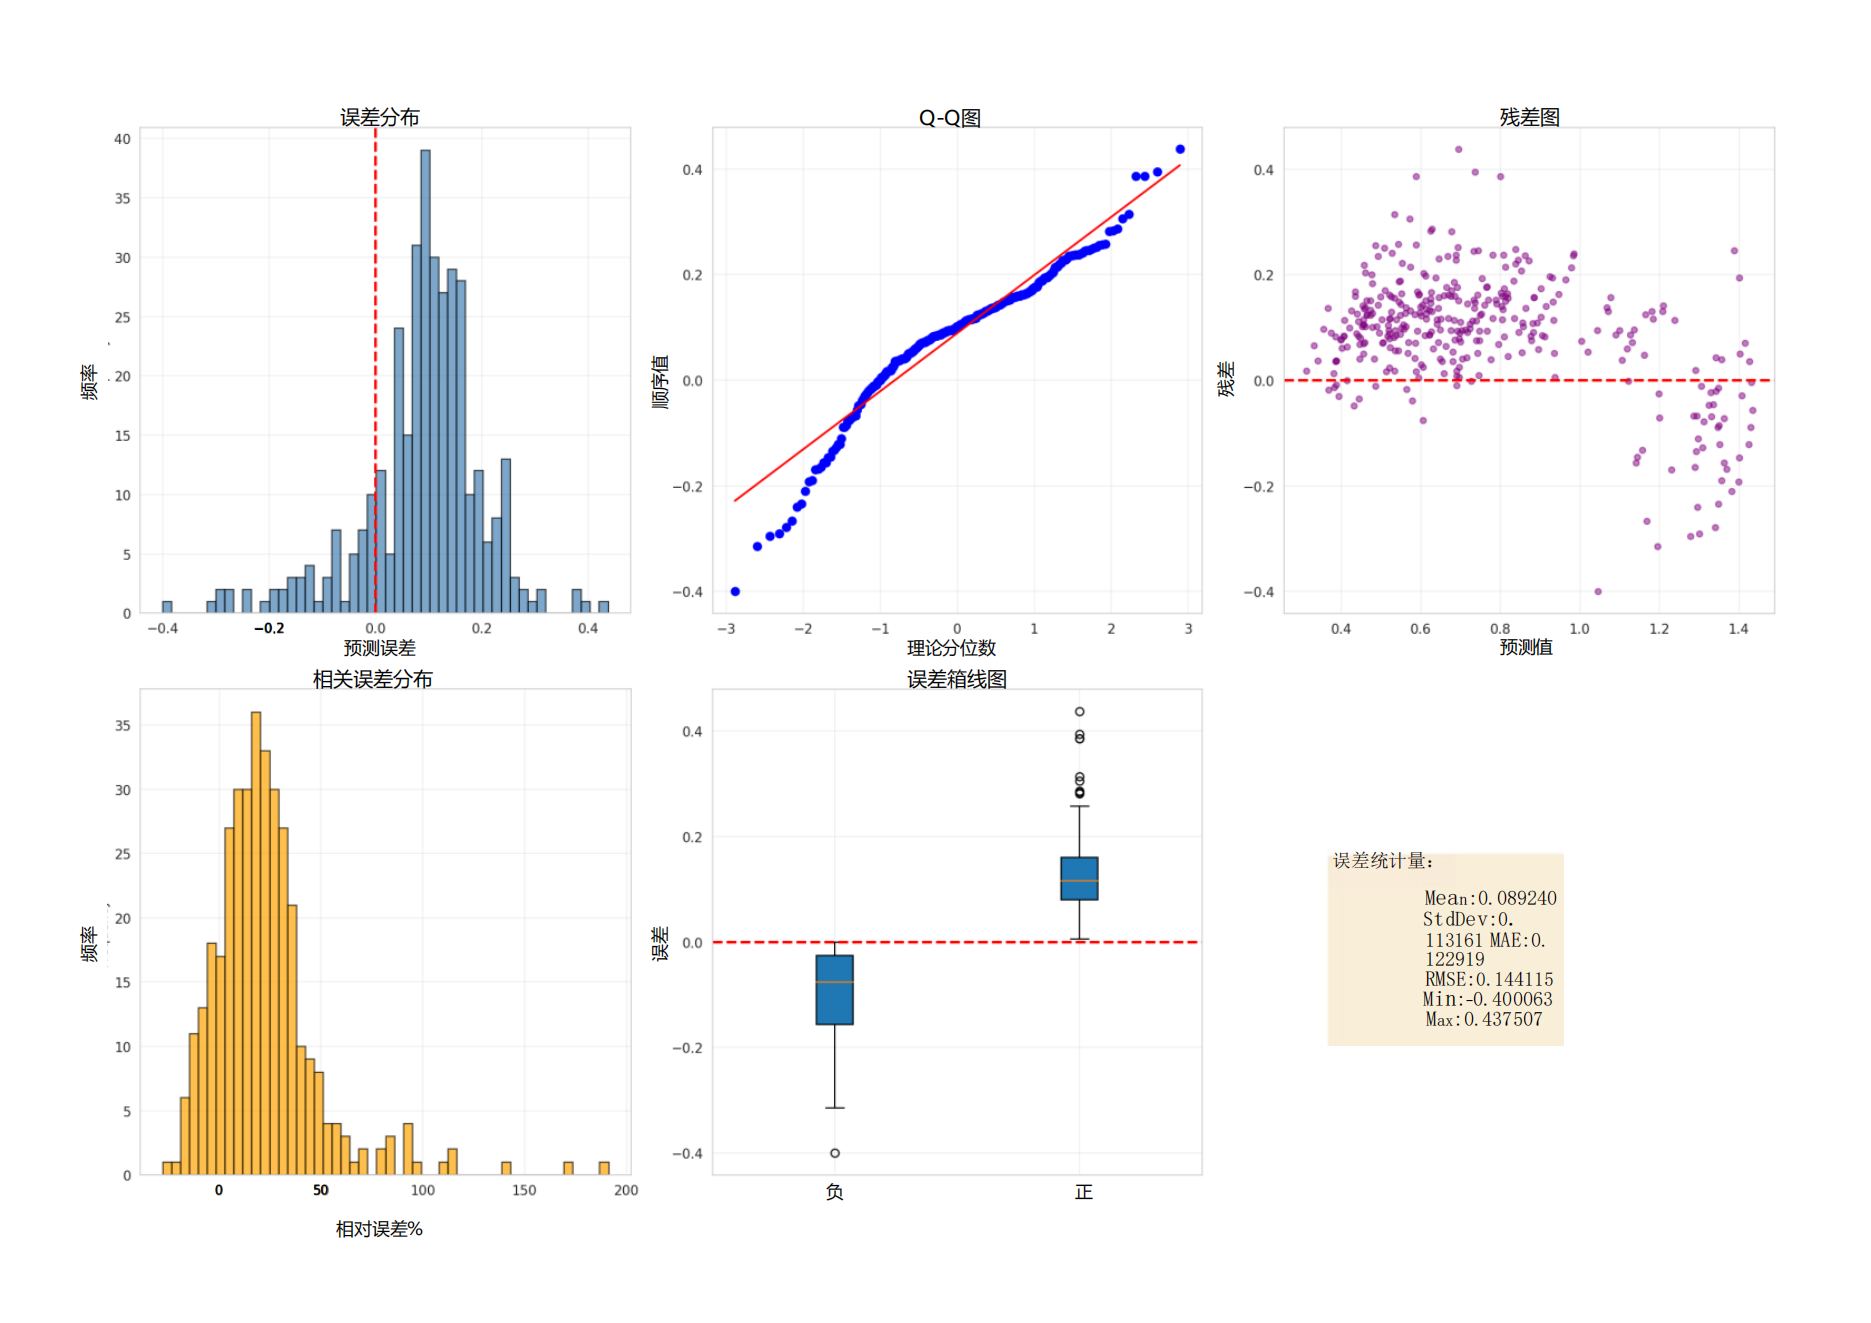
\includegraphics[width=0.80\textwidth]{figures/chap6/au_seg1_exp7_full_mgca_twin_error_analysis.png}
\caption{孪生对抗框架在黄金期货上的误差分布分析}
\label{fig:au9999exp7twinerroranaly_new}
\end{figure}

图\ref{fig:au9999exp7twinerroranaly_new}显示，黄金期货上的预测误差总体接近正态分布，残差序列未见明显结构性偏差，说明模型并非依赖单次偶然命中获得执行优势，而是在误差分布质量上具有一定稳定性。
在预测误差之外，还需要观察模型内部是否存在可用于筛选和替换的性能差异。图\ref{fig:multigencompare_new}展示了教师生成器与学生生成器在验证集上的性能分化。

\begin{figure}[!htbp]
\centering
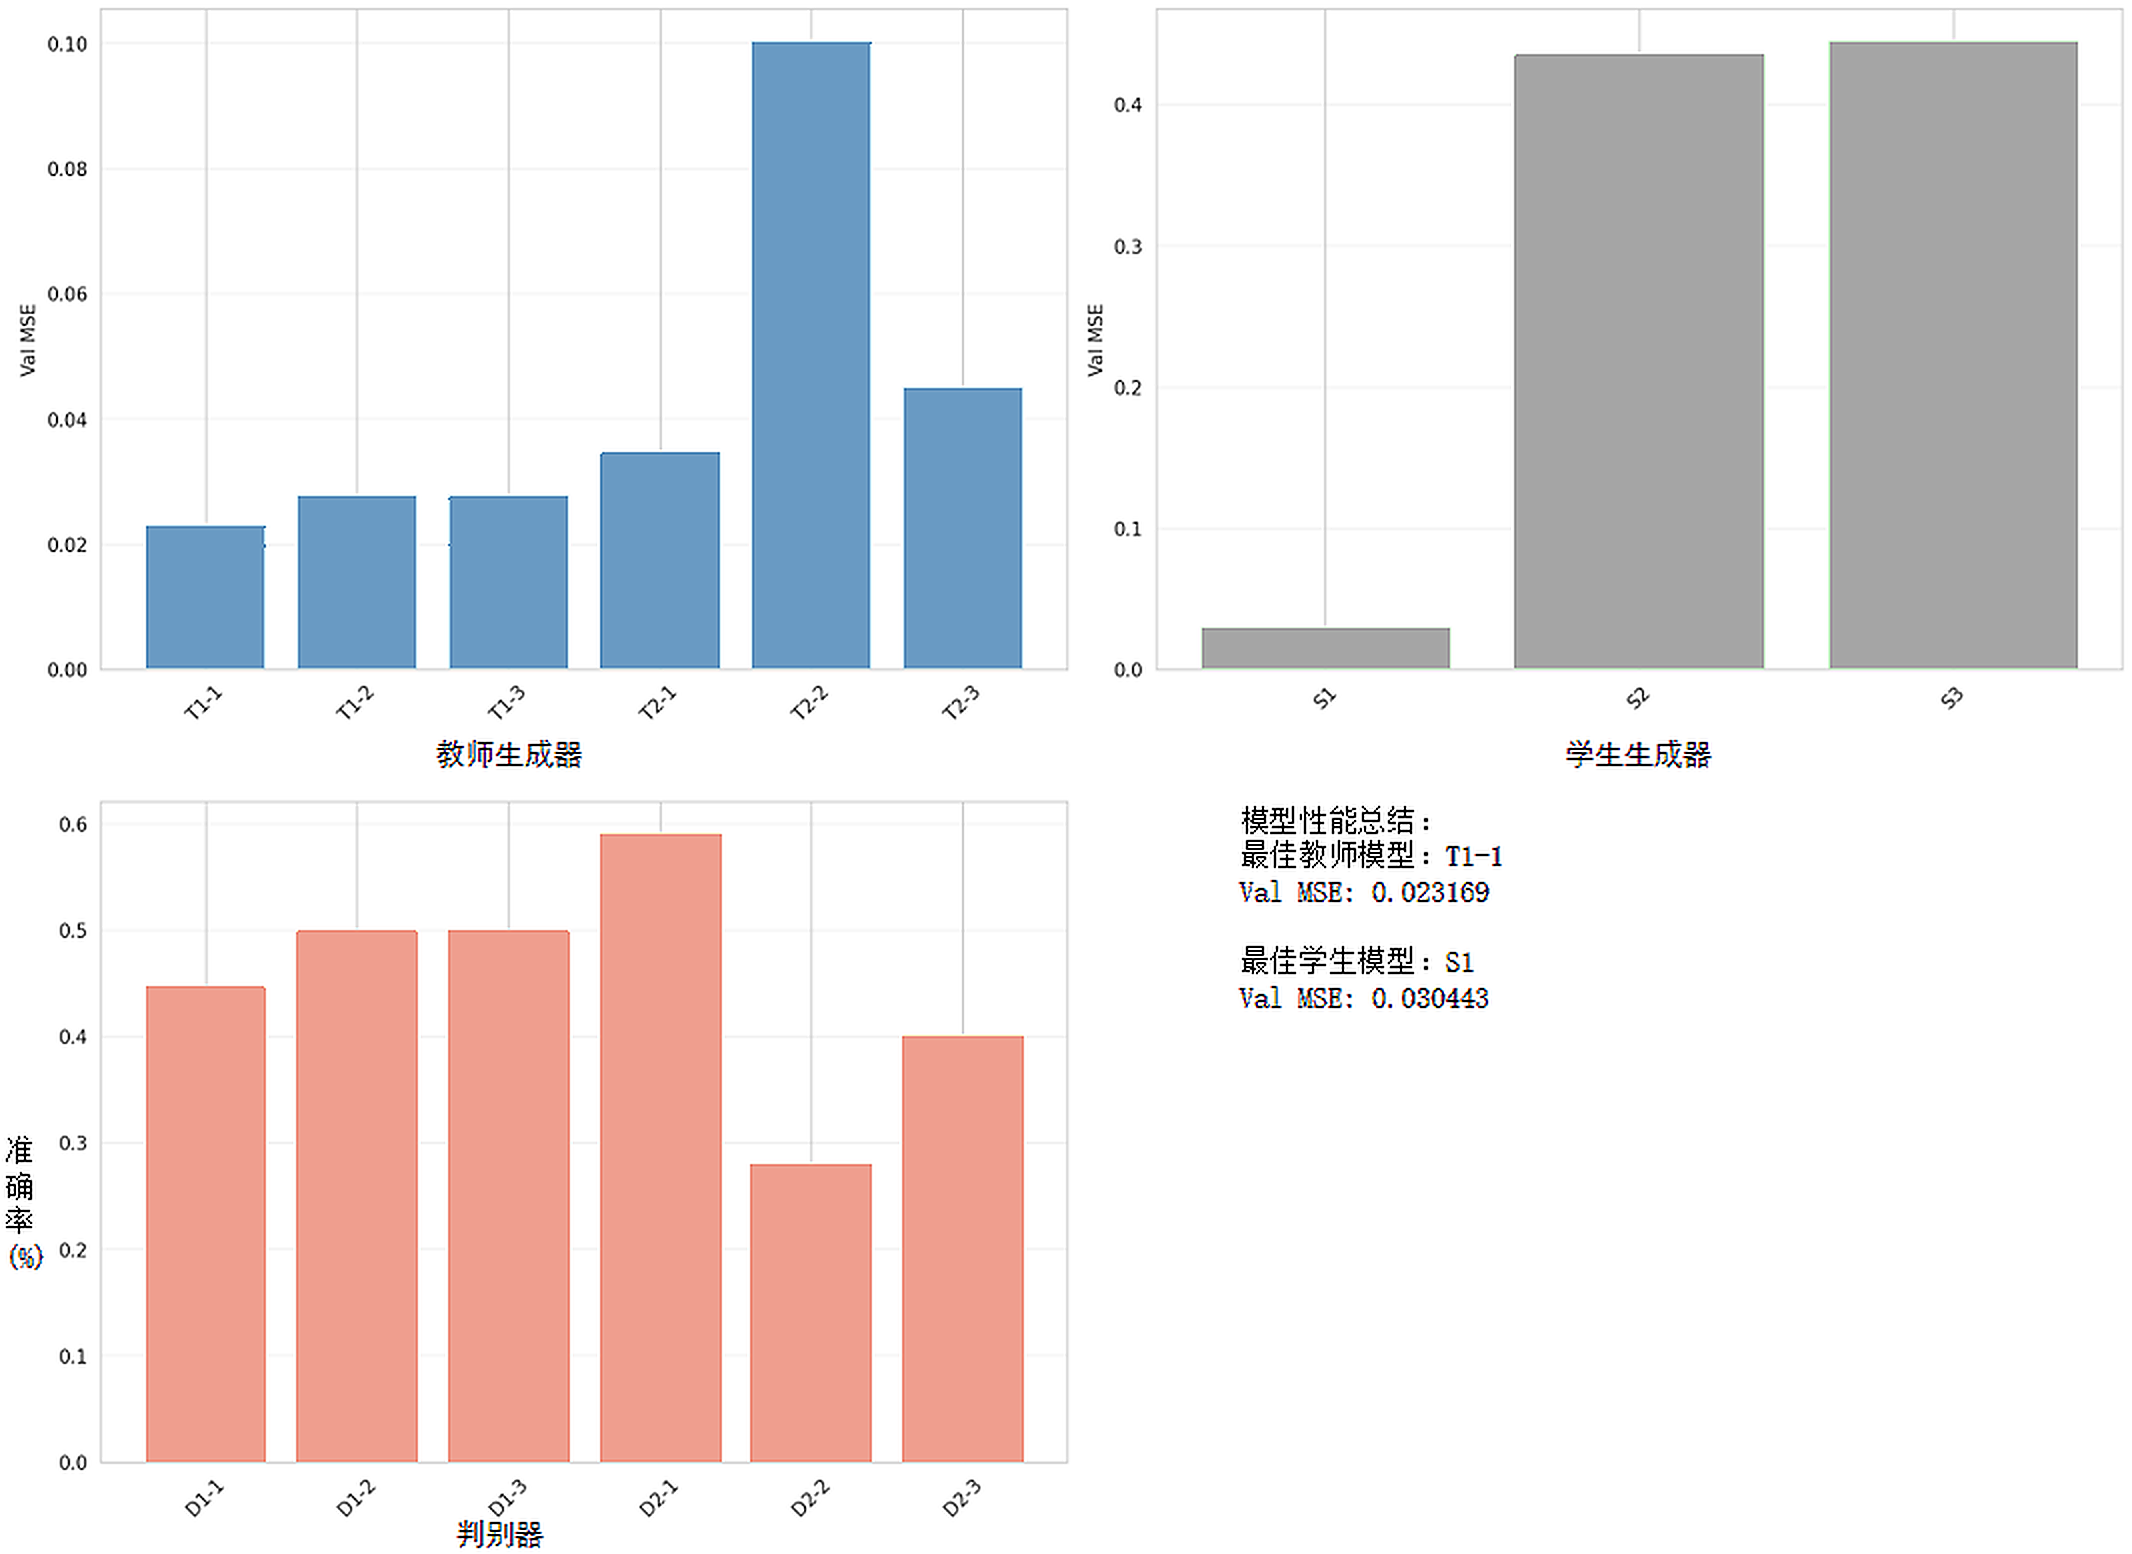
\includegraphics[width=0.80\textwidth]{figures/chap6/图5.9改.png}
\caption{孪生对抗框架在黄金期货（au数据集）上的多生成器性能对比}
\label{fig:multigencompare_new}
\end{figure}

不同成员的均方误差明显不同，这恰恰为赛马场竞争机制的动态选择和自体再生机制的偏离检测提供了基础：系统并不假定所有生成器都同样可靠，而是保留分化、比较与替换的空间。
在成员分化的基础上，图\ref{fig:au9999exp7twinvalmse_new}进一步展示了孪生对抗框架在验证集上的均方误差变化。

\begin{figure}[!htbp]
\centering
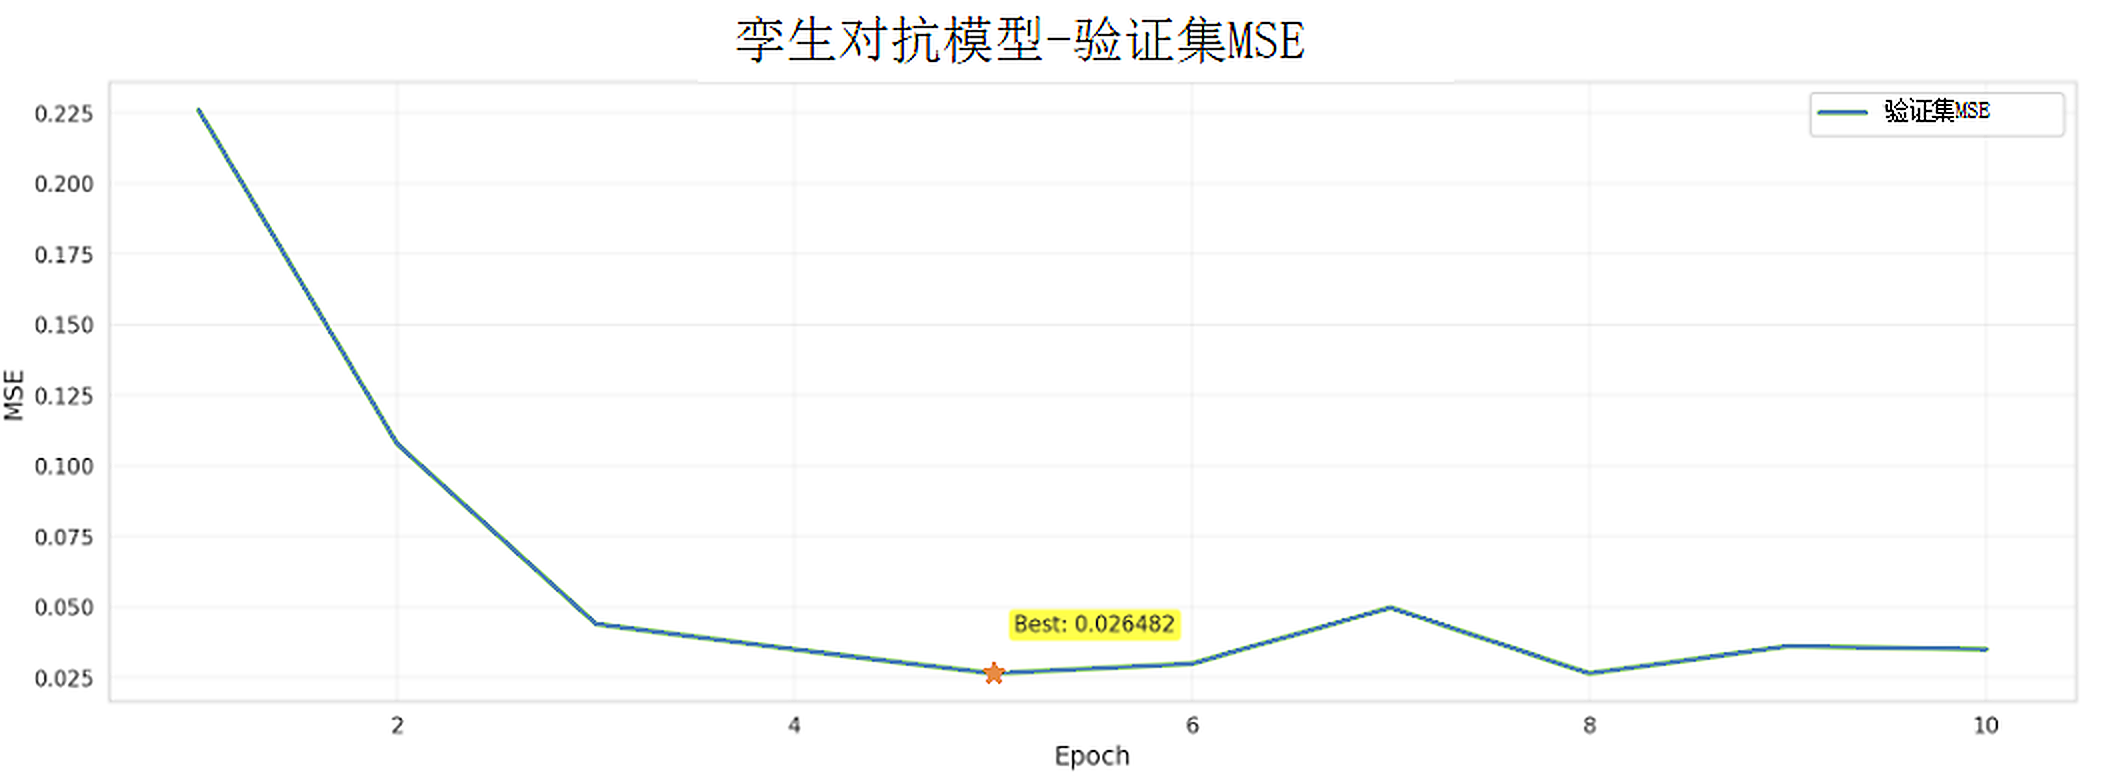
\includegraphics[width=0.80\textwidth]{figures/chap6/图5.10改.png}
\caption{孪生对抗框架在黄金期货验证集上的均方误差曲线}
\label{fig:au9999exp7twinvalmse_new}
\end{figure}

图\ref{fig:au9999exp7twinvalmse_new}表明，模型在 10 个 epoch 内较快收敛，并在第 5 个 epoch 左右达到较优泛化状态。训练过程中未出现明显崩溃，说明孪生对抗框架在该品种上表现出较好的训练稳定性。
最后转向成交量密度预测。图\ref{fig:au9999exp0baselinevolume_new}与图\ref{fig:au9999exp7twinvolume_new}分别给出基准模型和孪生对抗框架在黄金期货数据集上的成交量预测分析，用于观察模型输出能否进一步服务于订单拆分。

\begin{figure}[!htbp]
\centering
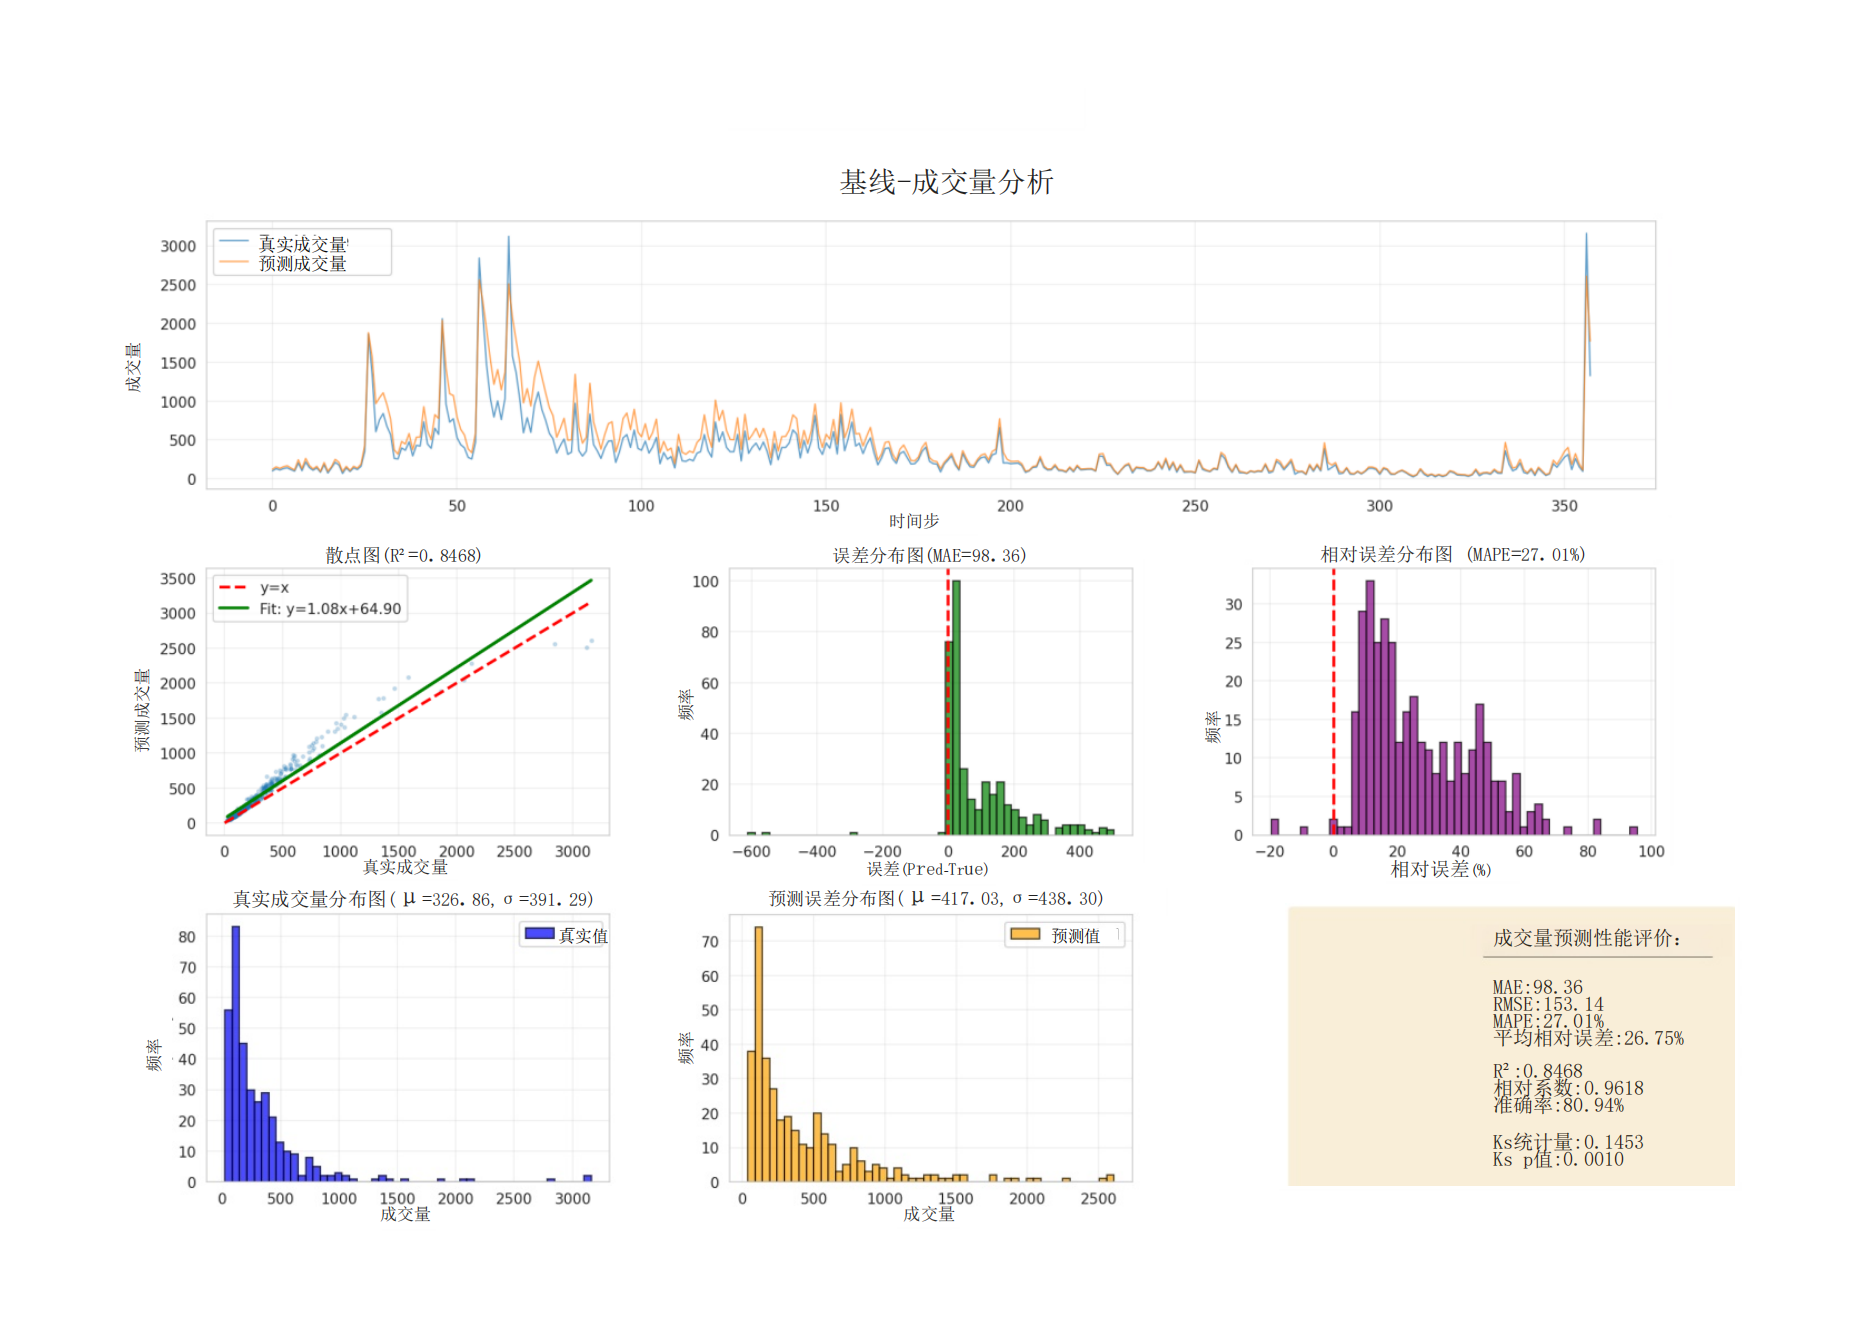
\includegraphics[width=0.80\textwidth]{figures/chap6/au_seg2_exp0_baseline_volume_analysis.png}
\caption{基准模型在黄金期货数据集上的成交量预测分析}
\label{fig:au9999exp0baselinevolume_new}
\end{figure}

\begin{figure}[!htbp]
\centering
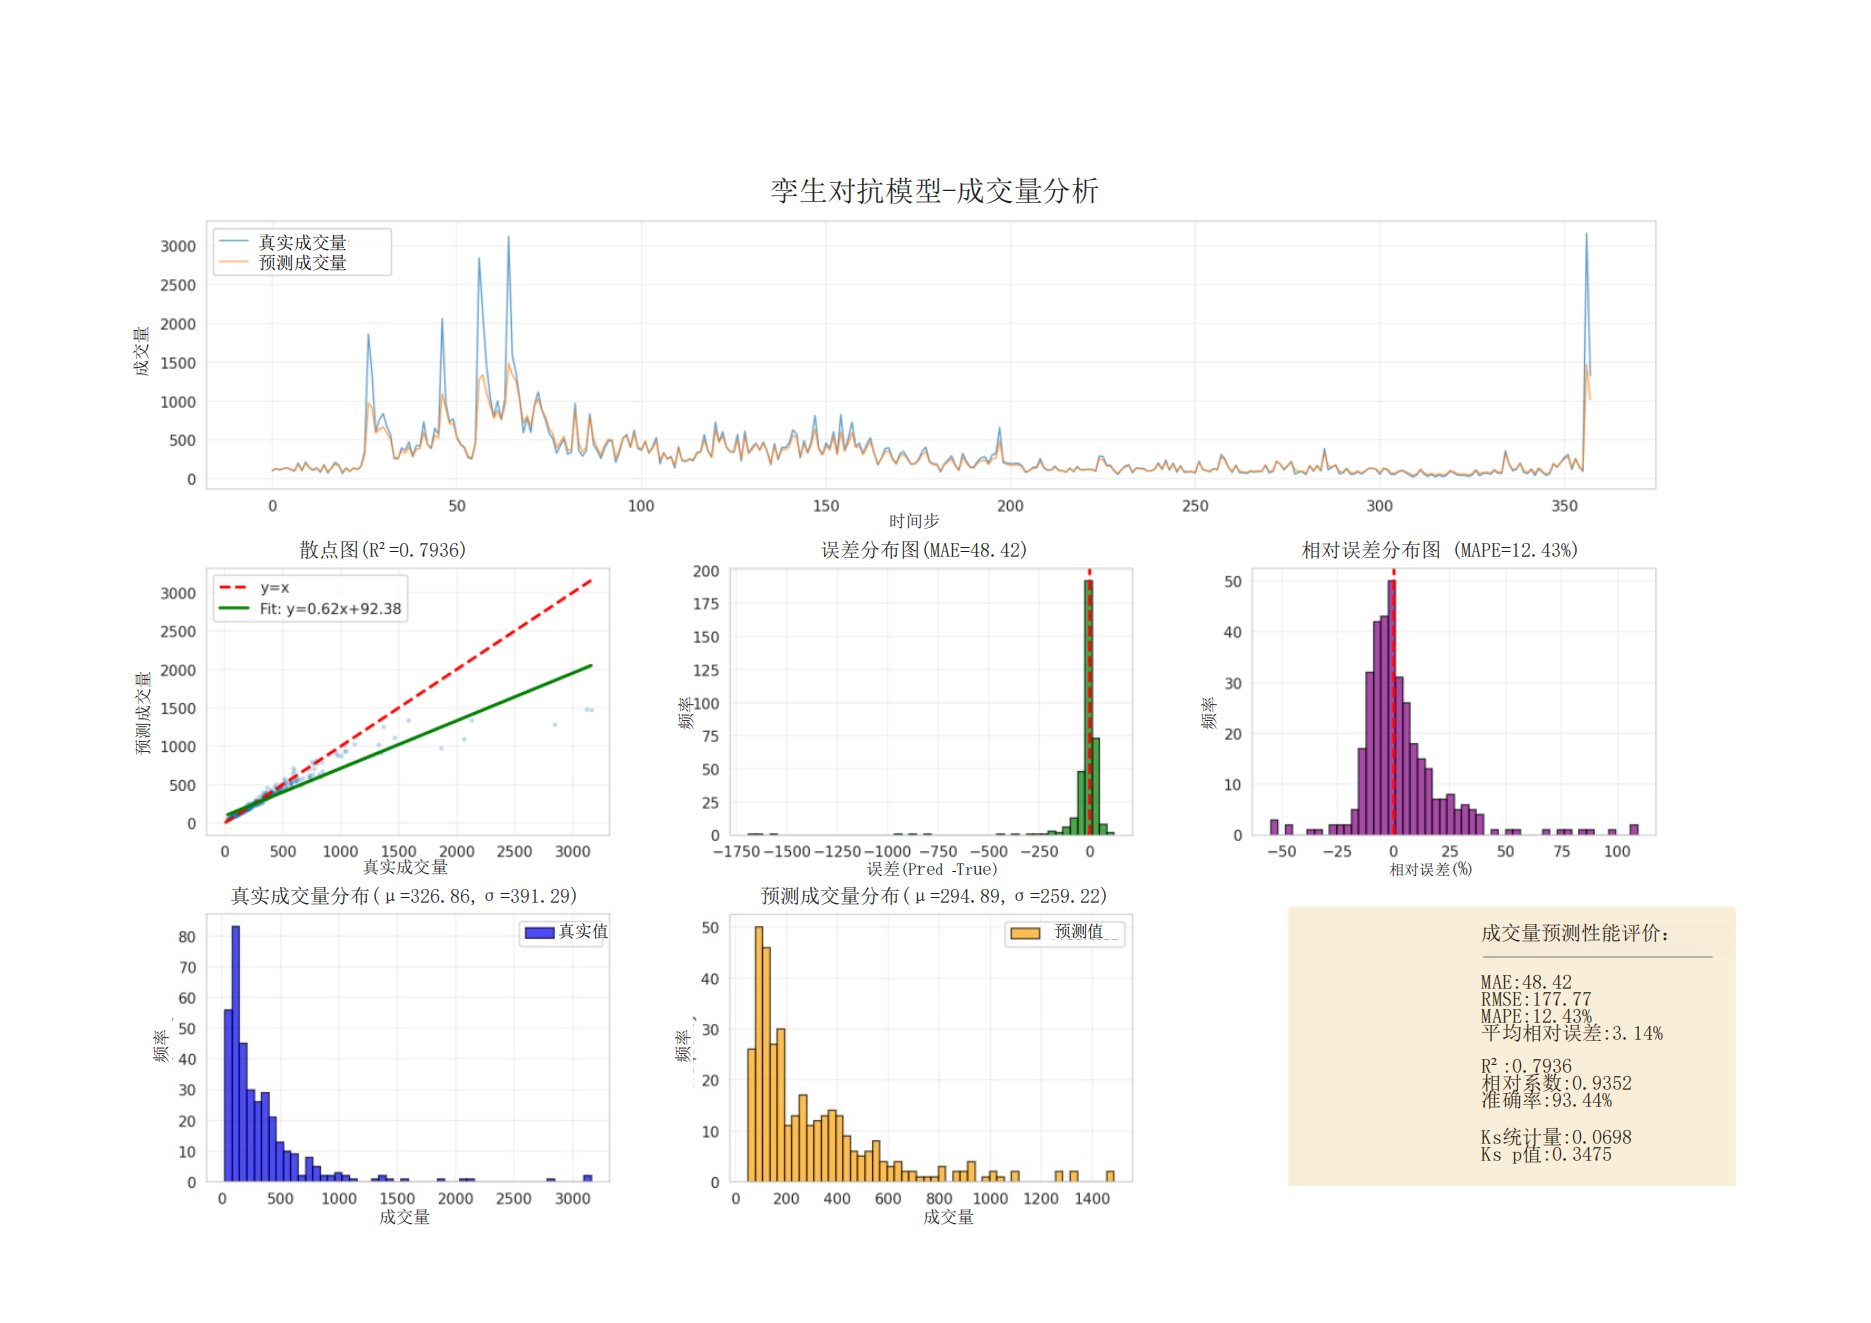
\includegraphics[width=0.80\textwidth]{figures/chap6/au_seg2_exp7_full_mgca_twin_volume_analysis.png}
\caption{孪生对抗框架在黄金期货数据集上的成交量预测分析}
\label{fig:au9999exp7twinvolume_new}
\end{figure}

图\ref{fig:au9999exp0baselinevolume_new}与图\ref{fig:au9999exp7twinvolume_new}说明，两种模型都能刻画成交量的基础趋势，但孪生对抗在峰值放量、突发缩量以及散点分布集中度上更集中。这一点对成交量加权平均价格执行较为重要，因为订单分配的好坏，本质上取决于模型是否在流动性最关键的分钟级节点上给出更可靠的成交量权重。高频市场分类中的长短期记忆网络集成研究表明，多模型结构有助于提高噪声市场中的短期方向识别能力\cite{borovkova2019ensemble}。这也解释了为什么本章不直接采用单一成交量预测器，而是通过候选生成、孪生校验和动态调度共同形成执行路径。

上述价格预测、误差分布、训练曲线和成交量预测结果共同说明，孪生对抗框架的优势并不只体现在单一预测误差下降上，更体现在局部结构识别、候选主体筛选和成交量密度刻画之间的协同。为使后续绩效表格与前述预测结果形成衔接，以下先从收益率与胜率两个直接执行指标入手，再逐步转向风险收益和连续性指标。

\FloatBarrier

% \begin{sidewaystable}
% \begin{table}
% \centering
% \footnotesize
% \setlength{\tabcolsep}{3pt}
% \begin{longtable}{lccccccccc}
% \caption{核心收益与胜率指标对比} \label{tab:twinreturnWinrate_new} \\
% \toprule


% \textbf{品种} & \textbf{时间} & \textbf{孪生对抗} & \textbf{Baseline} & \textbf{收益率} & \textbf{孪生对抗} & \textbf{Baseline} & \textbf{孪生对抗} & \textbf{Baseline} & \textbf{胜率} \\
%  & \textbf{段数} & \textbf{平均收益率} & \textbf{平均收益率} & \textbf{改善} & \textbf{年化收益率} & \textbf{年化收益率} & \textbf{胜率} & \textbf{胜率} & \textbf{提升} \\
%  & & \textbf{(\%)} & \textbf{(\%)} & \textbf{(\%)} & \textbf{(\%)} & \textbf{(\%)} & \textbf{(\%)} & \textbf{(\%)} & \textbf{(\%)} \\
% \midrule
% \endfirsthead
% \multicolumn{10}{c}{\tablename\ \thetable\ -- 续表} \\
% \toprule
% \textbf{品种} & \textbf{段数} & \textbf{孪生对抗平均} & \textbf{Baseline平均} & \textbf{收益率} & \textbf{孪生对抗年化} & \textbf{Baseline年化} & \textbf{孪生对抗} & \textbf{Baseline} & \textbf{胜率} \\
%  & & \textbf{收益率} & \textbf{收益率} & \textbf{改善} & \textbf{收益率} & \textbf{收益率} & \textbf{胜率} & \textbf{胜率} & \textbf{提升} \\
%  & & \textbf{(\%)} & \textbf{(\%)} & \textbf{(\%)} & \textbf{(\%)} & \textbf{(\%)} & \textbf{(\%)} & \textbf{(\%)} & \textbf{(\%)} \\
% \midrule
% \endhead
% \bottomrule
% \multicolumn{10}{p{0.95\textwidth}}{\footnotesize\textbf{注}：年化收益率 = 平均收益率 × 3125（年化倍数 3125 = 每日12.4个窗口 × 252交易日）。表中“年化收益率”为执行效率的年度等效百分比，非账户复利增长。}\\
% \endlastfoot
% 上证50股指 & 12 & 0.0590 & 0.0323 & 0.0267 & 184.50 & 100.96 & 58.3 & 50.0 & 8.3 \\
% 尿素 & 9 & 0.0310 & 0.0277 & 0.0034 & 97.01 & 86.45 & 66.7 & 66.7 & 0.0 \\
% 原油 & 21 & 0.0174 & -0.0058 & 0.0232 & 54.53 & -18.02 & 57.1 & 33.3 & 23.8 \\
% 沪深300股指 & 16 & 0.0162 & -0.0001 & 0.0163 & 50.59 & -0.46 & 56.2 & 43.8 & 12.5 \\
% 豆粕 & 14 & 0.0150 & 0.0056 & 0.0094 & 46.93 & 17.41 & 50.0 & 57.1 & -7.1 \\
% PTA & 14 & 0.0140 & 0.0023 & 0.0118 & 43.89 & 7.10 & 50.0 & 42.9 & 7.1 \\
% 铁矿石 & 14 & 0.0138 & 0.0058 & 0.0080 & 43.12 & 18.11 & 71.4 & 50.0 & 21.4 \\
% 玉米 & 14 & 0.0115 & 0.0034 & 0.0081 & 36.02 & 10.69 & 64.3 & 50.0 & 14.3 \\
% 液化石油气 & 14 & 0.0032 & 0.0018 & 0.0014 & 9.98 & 5.68 & 50.0 & 64.3 & -14.3 \\
% 苹果 & 9 & 0.0026 & 0.0057 & -0.0032 & 8.02 & 17.95 & 66.7 & 66.7 & 0.0 \\
% 镍 & 18 & 0.0018 & -0.0021 & 0.0039 & 5.50 & -6.60 & 66.7 & 44.4 & 22.2 \\
% 螺纹钢 & 14 & 0.0017 & 0.0071 & -0.0054 & 5.32 & 22.09 & 50.0 & 71.4 & -21.4 \\
% 菜籽油 & 14 & 0.0001 & -0.0013 & 0.0014 & 0.43 & -3.93 & 35.7 & 28.6 & 7.1 \\
% 10年期国债 & 10 & -0.0008 & -0.0008 & 0.0000 & -2.39 & -2.46 & 30.0 & 40.0 & -10.0 \\
% 黄金 & 22 & -0.0069 & -0.0245 & 0.0176 & -21.61 & -76.54 & 50.0 & 40.9 & 9.1 \\
% 棉花 & 14 & -0.0142 & -0.0057 & -0.0084 & -44.30 & -17.90 & 42.9 & 35.7 & 7.1 \\
% 铜 & 18 & -0.0175 & -0.0023 & -0.0151 & -54.65 & -7.33 & 38.9 & 50.0 & -11.1 \\
% 豆油 & 14 & -0.0183 & -0.0082 & -0.0101 & -57.25 & -25.74 & 21.4 & 28.6 & -7.1 \\
% 白银 & 22 & -0.0823 & -0.0344 & -0.0480 & -257.29 & -107.42 & 40.9 & 50.0 & -9.1 \\
% \end{longtable}
% % \end{sidewaystable}
% \end{table}
\begin{table}[!htbp]
\centering
\caption{核心收益与胜率指标对比}
\label{tab:core_compare}
\footnotesize
\setlength{\tabcolsep}{2pt}
\renewcommand{\arraystretch}{1.18}
\begin{tabular}{@{}p{0.12\textwidth}p{0.055\textwidth}p{0.13\textwidth}p{0.13\textwidth}p{0.105\textwidth}p{0.13\textwidth}p{0.13\textwidth}@{}}
\toprule
\textbf{品种} &
\makecell{\textbf{时间}\\\textbf{段数}} &
\makecell{\textbf{孪生对抗}\\\textbf{平均}\\\textbf{收益率(\%)}} &
\makecell{\textbf{基准模型}\\\textbf{平均}\\\textbf{收益率(\%)}} &
\makecell{\textbf{收益率}\\\textbf{改善(\%)}} &
\makecell{\textbf{孪生对抗}\\\textbf{年化}\\\textbf{收益率(\%)}} &
\makecell{\textbf{基准模型}\\\textbf{年化}\\\textbf{收益率(\%)}} \\
\midrule
上证50股指 & 12 & 0.0590 & 0.0323 & 0.0267 & 184.50 & 100.96 \\
尿素 & 9 & 0.0310 & 0.0277 & 0.0034 & 97.01 & 86.45 \\
原油 & 21 & 0.0174 & -0.0058 & 0.0232 & 54.53 & -18.02 \\
沪深300股指 & 16 & 0.0162 & -0.0001 & 0.0163 & 50.59 & -0.46 \\
豆粕 & 14 & 0.0150 & 0.0056 & 0.0094 & 46.93 & 17.41 \\
PTA & 14 & 0.0140 & 0.0023 & 0.0118 & 43.89 & 7.10 \\
铁矿石 & 14 & 0.0138 & 0.0058 & 0.0080 & 43.12 & 18.11 \\
玉米 & 14 & 0.0115 & 0.0034 & 0.0081 & 36.02 & 10.69 \\
液化石油气 & 14 & 0.0032 & 0.0018 & 0.0014 & 9.98 & 5.68 \\
苹果 & 9 & 0.0026 & 0.0057 & -0.0032 & 8.02 & 17.95 \\
镍 & 18 & 0.0018 & -0.0021 & 0.0039 & 5.50 & -6.60 \\
螺纹钢 & 14 & 0.0017 & 0.0071 & -0.0054 & 5.32 & 22.09 \\
菜籽油 & 14 & 0.0001 & -0.0013 & 0.0014 & 0.43 & -3.93 \\
10年期国债 & 10 & -0.0008 & -0.0008 & 0.0000 & -2.39 & -2.46 \\
黄金 & 22 & -0.0069 & -0.0245 & 0.0176 & -21.61 & -76.54 \\
棉花 & 14 & -0.0142 & -0.0057 & -0.0084 & -44.30 & -17.90 \\
铜 & 18 & -0.0175 & -0.0023 & -0.0151 & -54.65 & -7.33 \\
豆油 & 14 & -0.0183 & -0.0082 & -0.0101 & -57.25 & -25.74 \\
白银 & 22 & -0.0823 & -0.0344 & -0.0480 & -257.29 & -107.42 \\
\bottomrule
\end{tabular}
\end{table}
\begin{table}[!htbp]
\centering
{\small\textbf{续表}}\\[0.5em]
\footnotesize
\setlength{\tabcolsep}{3pt}
\renewcommand{\arraystretch}{1.18}
\begin{tabular}{@{}p{0.16\textwidth}p{0.18\textwidth}p{0.18\textwidth}p{0.18\textwidth}p{0.14\textwidth}@{}}
\toprule
\textbf{品种} & \textbf{时间段数} & \makecell{\textbf{孪生对抗}\\\textbf{胜率(\%)}} & \makecell{\textbf{基准模型}\\\textbf{胜率(\%)}} & \makecell{\textbf{胜率}\\\textbf{提升(\%)}} \\
\midrule
上证50股指 & 12 & 58.3 & 50.0 & 8.3 \\
尿素 & 9 & 66.7 & 66.7 & 0.0 \\
原油 & 21 & 57.1 & 33.3 & 23.8 \\
沪深300股指 & 16 & 56.2 & 43.8 & 12.5 \\
豆粕 & 14 & 50.0 & 57.1 & -7.1 \\
PTA & 14 & 50.0 & 42.9 & 7.1 \\
铁矿石 & 14 & 71.4 & 50.0 & 21.4 \\
玉米 & 14 & 64.3 & 50.0 & 14.3 \\
液化石油气 & 14 & 50.0 & 64.3 & -14.3 \\
苹果 & 9 & 66.7 & 66.7 & 0.0 \\
镍 & 18 & 66.7 & 44.4 & 22.2 \\
螺纹钢 & 14 & 50.0 & 71.4 & -21.4 \\
菜籽油 & 14 & 35.7 & 28.6 & 7.1 \\
10年期国债 & 10 & 30.0 & 40.0 & -10.0 \\
黄金 & 22 & 50.0 & 40.9 & 9.1 \\
棉花 & 14 & 42.9 & 35.7 & 7.1 \\
铜 & 18 & 38.9 & 50.0 & -11.1 \\
豆油 & 14 & 21.4 & 28.6 & -7.1 \\
白银 & 22 & 40.9 & 50.0 & -9.1 \\
\bottomrule
\end{tabular}
\end{table}

表\ref{tab:core_compare}给出了收益率与胜率的对比结果。总体上，19 个品种中有 12 个在平均收益率维度获得改善，上证50股指、原油、沪深300股指、PTA 和铁矿石等品种表现尤为突出。其中，上证50股指的每 30 分钟平均收益率达到 0.0590\%，对应年化等效 184.50\%；原油和沪深300股指则实现了从基准模型负收益到该机制正收益的转变。相较之下，白银、铜和豆油等高噪声品种仍然表现较弱，提示机制存在明确的适用边界。

在收益率与胜率之外，还需要进一步观察收益是否伴随过高回撤或下行波动。如果执行优化只提升局部收益而同步放大尾部风险，则难以作为稳定执行模块嵌入真实交易系统。因此，表\ref{tab:twinriskReturn_new}进一步给出盈亏比、最大回撤、夏普比率与卡玛比率等风险收益指标。

\FloatBarrier

% \begin{sidewaystable}
\begin{table}[!htbp]
\centering
\caption{风险收益比指标对比}
\label{tab:twinriskReturn_new}
\small
\setlength{\tabcolsep}{6pt}
\renewcommand{\arraystretch}{1.18}
\begin{tabular}{lcccc}
\toprule
\textbf{品种} & \makecell{\textbf{孪生对抗}\\\textbf{盈亏比}} & \makecell{\textbf{基准模型}\\\textbf{盈亏比}} & \makecell{\textbf{孪生对抗}\\\textbf{最大回撤(\%)}} & \makecell{\textbf{基准模型}\\\textbf{最大回撤(\%)}} \\
\midrule
上证50股指 & 10.57 & 6.65 & 41.17 & 100.00 \\
尿素 & 1.30 & 4.85 & 42.12 & 15.07 \\
原油 & 2.01 & 1.15 & 100.00 & 88.03 \\
沪深300股指 & 1.93 & 1.27 & 90.82 & 100.00 \\
豆粕 & 2.35 & 1.49 & 100.00 & 100.00 \\
PTA & 1.95 & 1.69 & 91.69 & 84.17 \\
铁矿石 & 0.66 & 1.83 & 82.61 & 86.51 \\
玉米 & 1.31 & 1.91 & 28.39 & 60.25 \\
液化石油气 & 1.23 & 0.78 & 100.00 & 100.00 \\
苹果 & 0.58 & 0.86 & 100.00 & 100.00 \\
镍 & 0.60 & 0.94 & 86.25 & 100.00 \\
螺纹钢 & 1.17 & 1.27 & 77.61 & 59.32 \\
菜籽油 & 1.81 & 2.17 & 97.10 & 100.00 \\
10年期国债 & 1.37 & 0.88 & 100.00 & 100.00 \\
黄金 & 0.63 & 0.18 & 100.00 & 100.00 \\
棉花 & 0.43 & 0.55 & 100.00 & 100.00 \\
铜 & 0.34 & 0.56 & 87.95 & 83.11 \\
豆油 & 0.34 & 1.31 & 100.00 & 100.00 \\
白银 & 0.14 & 0.16 & 100.00 & 100.00 \\
\bottomrule
\end{tabular}
\end{table}
\begin{table}[!htbp]
\centering
{\small\textbf{续表}}\\[0.5em]
\small
\setlength{\tabcolsep}{7pt}
\renewcommand{\arraystretch}{1.18}
\begin{tabular}{lcccc}
\toprule
\textbf{品种} & \makecell{\textbf{孪生对抗}\\\textbf{夏普比率}} & \makecell{\textbf{基准模型}\\\textbf{夏普比率}} & \makecell{\textbf{孪生对抗}\\\textbf{卡玛比率}} & \makecell{\textbf{基准模型}\\\textbf{卡玛比率}} \\
\midrule
上证50股指 & 31.05 & 18.03 & 4.48 & 1.01 \\
尿素 & 15.40 & 39.88 & 2.30 & 5.74 \\
原油 & 14.64 & -11.32 & 0.55 & -0.20 \\
沪深300股指 & 18.51 & -0.23 & 0.56 & -0.00 \\
豆粕 & 14.75 & 13.43 & 0.47 & 0.17 \\
PTA & 12.12 & 4.75 & 0.48 & 0.08 \\
铁矿石 & 9.12 & 11.61 & 0.52 & 0.21 \\
玉米 & 18.15 & 14.64 & 1.27 & 0.18 \\
液化石油气 & 3.32 & 7.24 & 0.10 & 0.06 \\
苹果 & 3.01 & 9.59 & 0.08 & 0.18 \\
镍 & 3.66 & -5.76 & 0.06 & -0.07 \\
螺纹钢 & 3.07 & 22.41 & 0.07 & 0.37 \\
菜籽油 & 0.10 & -2.55 & 0.00 & -0.04 \\
10年期国债 & -10.77 & -12.05 & -0.02 & -0.02 \\
黄金 & -8.03 & -16.03 & -0.22 & -0.77 \\
棉花 & -19.82 & -22.28 & -0.44 & -0.18 \\
铜 & -21.69 & -12.01 & -0.62 & -0.09 \\
豆油 & -36.70 & -10.80 & -0.57 & -0.26 \\
白银 & -15.09 & -13.64 & -2.57 & -1.07 \\
\bottomrule
\end{tabular}
\end{table}

表\ref{tab:twinriskReturn_new}揭示了更细粒度的风险收益结构。上证50股指在盈亏比、夏普比率和卡玛比率三个维度上同时领先，说明其高收益并非来自偶然命中，而是建立在较优风险控制基础之上；玉米的最大回撤仅为 28.39\%，在风险控制维度表现突出；原油与沪深300股指则实现了夏普比率由负转正。与此同时，若干品种的最大回撤仍达到 100\%，说明在极端高噪声条件下，孪生对抗虽能改善执行效率，但尚不能完全消除尾部风险。
风险收益指标反映的是整体分布特征，尚不能完全说明盈利或亏损在时间序列中的连续性。为进一步判断执行路径是否容易出现连续失效，表\ref{tab:twinadvancedMetrics_new}从下行风险和连胜连亏角度补充检验。

\FloatBarrier

% \begin{sidewaystable}
\begin{table}[!htbp]
\centering
\caption{高级绩效指标对比}
\label{tab:twinadvancedMetrics_new}
\small
\setlength{\tabcolsep}{5pt}
\renewcommand{\arraystretch}{1.18}
\begin{tabular}{lcccccc}
\toprule
\textbf{品种} & \makecell{\textbf{孪生对抗}\\\textbf{索提诺比率}} & \makecell{\textbf{基准模型}\\\textbf{索提诺比率}} & \makecell{\textbf{孪生对抗}\\\textbf{最大连胜}} & \makecell{\textbf{孪生对抗}\\\textbf{最大连亏}} & \makecell{\textbf{基准模型}\\\textbf{最大连胜}} & \makecell{\textbf{基准模型}\\\textbf{最大连亏}} \\
\midrule
上证50股指 & 319.21 & 117.17 & 3 & 2 & 3 & 4 \\
尿素 & 44.22 & 162.03 & 3 & 2 & 4 & 2 \\
原油 & 38.82 & -15.98 & 3 & 3 & 3 & 6 \\
沪深300股指 & 33.80 & -0.36 & 3 & 3 & 3 & 5 \\
豆粕 & 30.78 & 32.47 & 5 & 5 & 3 & 2 \\
PTA & 29.26 & 6.97 & 4 & 3 & 2 & 3 \\
铁矿石 & 8.87 & 17.54 & 5 & 2 & 4 & 3 \\
玉米 & 30.91 & 29.88 & 3 & 2 & 2 & 2 \\
液化石油气 & 3.79 & 10.11 & 4 & 3 & 5 & 3 \\
苹果 & 3.79 & 16.65 & 2 & 1 & 2 & 1 \\
\bottomrule
\end{tabular}
\end{table}
\begin{table}[!htbp]
\centering
{\small\textbf{续表}}\\[0.5em]
\small
\setlength{\tabcolsep}{5pt}
\renewcommand{\arraystretch}{1.18}
\begin{tabular}{lcccccc}
\toprule
\textbf{品种} & \makecell{\textbf{孪生对抗}\\\textbf{索提诺比率}} & \makecell{\textbf{基准模型}\\\textbf{索提诺比率}} & \makecell{\textbf{孪生对抗}\\\textbf{最大连胜}} & \makecell{\textbf{孪生对抗}\\\textbf{最大连亏}} & \makecell{\textbf{基准模型}\\\textbf{最大连胜}} & \makecell{\textbf{基准模型}\\\textbf{最大连亏}} \\
\midrule
镍 & 6.76 & -10.70 & 4 & 3 & 3 & 3 \\
螺纹钢 & 4.41 & 35.42 & 3 & 2 & 5 & 2 \\
菜籽油 & 0.21 & -7.93 & 2 & 4 & 1 & 5 \\
10年期国债 & -25.40 & -33.62 & 2 & 3 & 2 & 3 \\
黄金 & -8.72 & -12.86 & 3 & 6 & 4 & 5 \\
棉花 & -21.85 & -25.95 & 3 & 4 & 2 & 4 \\
铜 & -20.34 & -14.53 & 3 & 4 & 4 & 4 \\
豆油 & -38.31 & -20.77 & 2 & 7 & 1 & 5 \\
白银 & -11.95 & -10.05 & 3 & 4 & 4 & 5 \\
\bottomrule
\end{tabular}
\end{table}

表\ref{tab:twinadvancedMetrics_new}从下行风险与连续性维度补充了执行表现。上证50股指、原油、沪深300股指、豆粕、PTA 与玉米的索提诺比率较高，说明这些品种在控制下行波动方面优于整体波动表现；豆粕和铁矿石的最大连胜均达到 5，体现出盈利持续性；豆油的最大连亏为 7，则反映了高噪声品种在连续亏损压力上的约束。

在分别完成收益、风险与连续性指标分析后，图\ref{fig:comprehensiveviz_new}将上述评价维度集中呈现，用于辅助观察不同品种在多指标空间中的相对位置。

\FloatBarrier

\begin{figure}[!p]
\centering
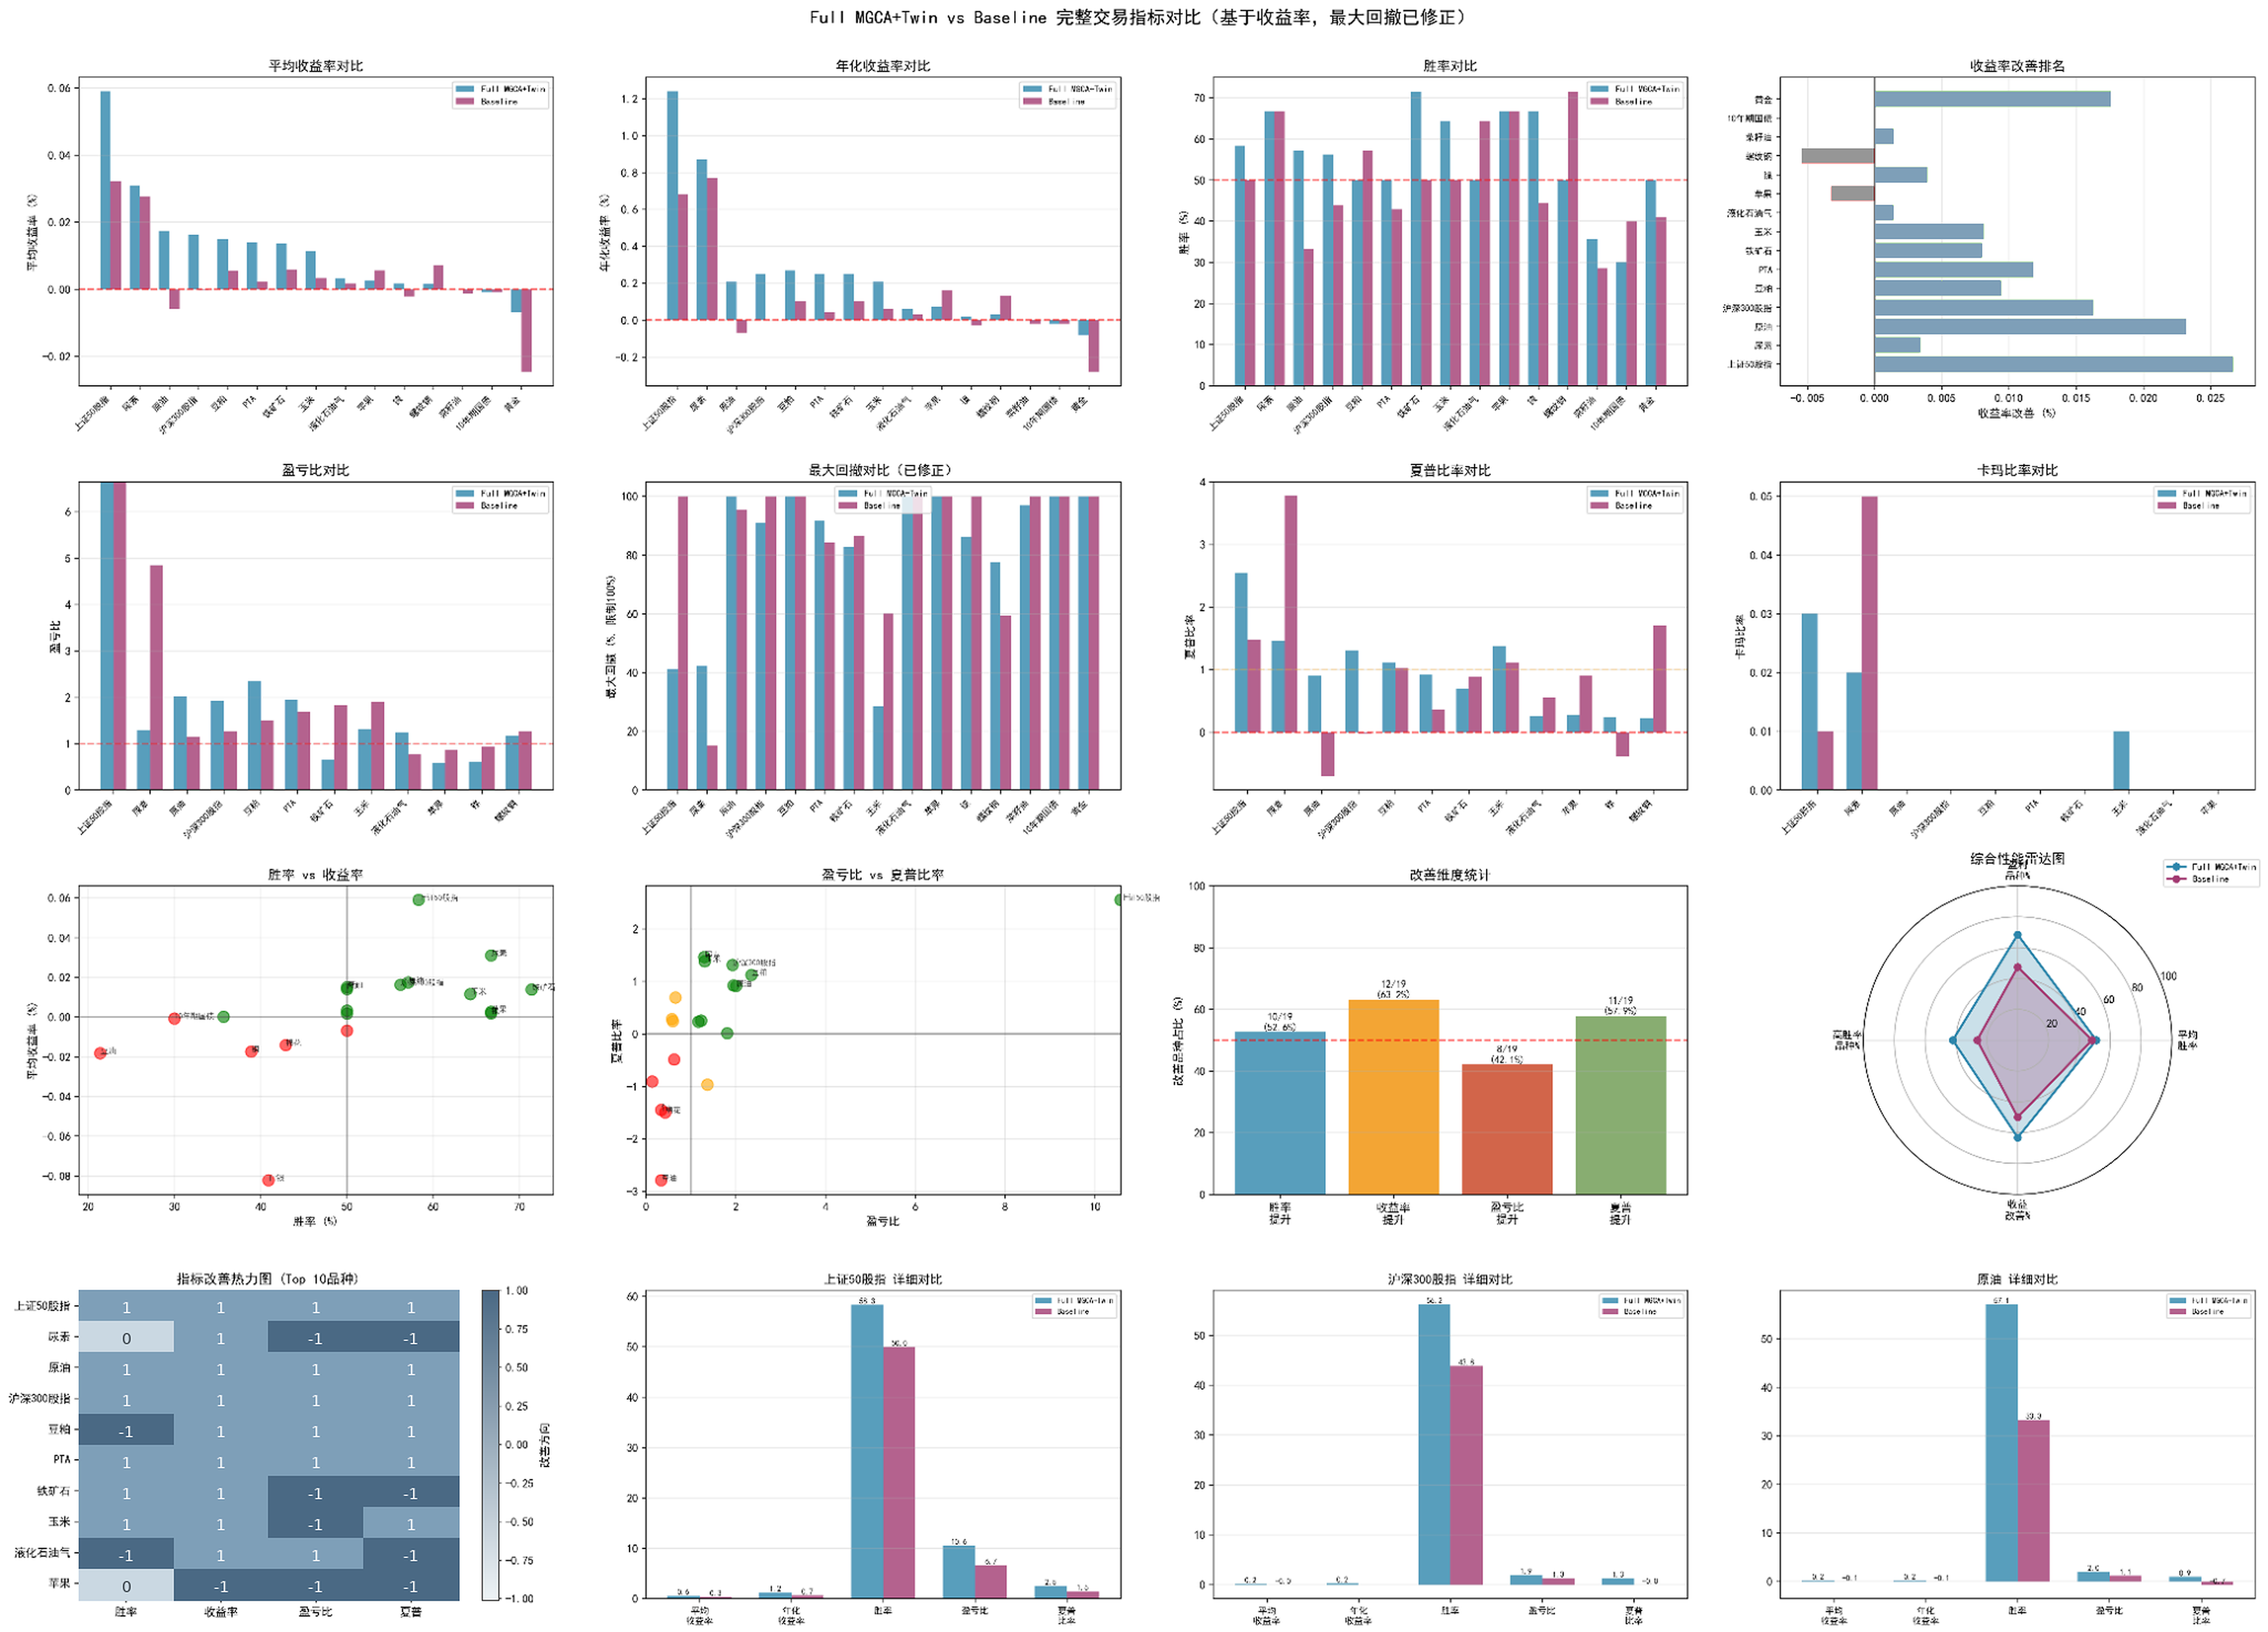
\includegraphics[width=0.96\textwidth]{figures/chap6/图5.13改.png}
\caption{孪生对抗框架综合交易指标对比可视化（16个子图综合分析）}
\label{fig:comprehensiveviz_new}
\end{figure}

图\ref{fig:comprehensiveviz_new}综合可视化了收益率、胜率、盈亏比、最大回撤、夏普比率、卡玛比率及改善热力图等结果。可视化结果与前述表格一致：上证50股指、沪深300股指和原油是多维度改善最明显的代表品种，而部分品种则呈现“某些指标改善、某些指标恶化”的混合特征，也说明执行模型的评价不能只看单一维度。
在多维绩效评价之后，仍需回到交易执行优化的直接目标，即成本改善是否能够在多个品种上稳定出现。表\ref{tab:advanced_performance_new}进一步汇总 19 个品种上的成本节省极值与整体表现，用于观察该机制的跨品种适用性和失效边界。

\FloatBarrier

\begin{table}[!htbp]
\centering
\caption{孪生对抗在19个品种上的成本节省极值与整体表现}
\label{tab:advanced_performance_new}
\small
\setlength{\tabcolsep}{6pt}
\renewcommand{\arraystretch}{1.18}
\begin{tabular}{lcccc}
\toprule
\multirow{2}{*}{\textbf{品种}} & \multicolumn{3}{c}{\textbf{孪生对抗成本(元)}} & \multirow{2}{*}{\makecell{\textbf{基准模型}\\\textbf{成本(元)}}} \\
\cmidrule(lr){2-4}
 & \textbf{平均} & \textbf{最高} & \textbf{最低} &  \\
\midrule
上证50股指 & 15,173 & 88,624 & -6,795 & 8,110 \\
沪深300股指 & 6,047 & 48,403 & -30,672 & -188 \\
10年期国债 & -8 & 95 & -53 & -9 \\
PTA & 6,729 & 92,986 & -40,644 & 1,115 \\
菜籽油 & 1,181 & 221,336 & -107,773 & -820 \\
原油 & 797 & 12,052 & -5,188 & -344 \\
液化石油气 & 1,730 & 56,820 & -58,038 & 832 \\
尿素 & 5,368 & 51,283 & -19,631 & 4,858 \\
铁矿石 & 1,114 & 12,234 & -14,794 & 454 \\
螺纹钢 & 713 & 21,700 & -18,408 & 2,254 \\
豆粕 & 4,660 & 51,155 & -23,239 & 1,672 \\
玉米 & 2,612 & 17,716 & -12,152 & 787 \\
苹果 & 1,431 & 51,264 & -58,590 & 4,456 \\
豆油 & -14,395 & 14,670 & -61,206 & -6,496 \\
棉花 & -18,933 & 78,230 & -140,355 & -7,631 \\
黄金 & -457 & 6,895 & -9,345 & -1,612 \\
白银 & -64,197 & 67,306 & -1,099,435 & -26,781 \\
镍 & 21,592 & 731,412 & -552,995 & -26,469 \\
铜 & -133,553 & 330,227 & -1,261,400 & -17,472 \\
\bottomrule
\end{tabular}
\end{table}
\begin{table}[!htbp]
\centering
{\small\textbf{续表}}\\[0.5em]
\small
\setlength{\tabcolsep}{5pt}
\renewcommand{\arraystretch}{1.18}
\begin{tabular}{lccccc}
\toprule
\multirow{2}{*}{\textbf{品种}} & \multicolumn{3}{c}{\textbf{成本改善(元)}} & \multirow{2}{*}{\makecell{\textbf{均方误差}\\\textbf{变化}}} & \multirow{2}{*}{\makecell{\textbf{盈利率}\\\textbf{(\%)}}} \\
\cmidrule(lr){2-4}
 & \textbf{平均} & \textbf{最高} & \textbf{最低} & & \\
\midrule
上证50股指 & \checkmark +7,063 & +23,753 & -3,398 & +14.0\% & 58.3 \\
沪深300股指 & \checkmark +6,235 & +42,716 & -23,236 & +29.8\% & 56.2 \\
10年期国债 & \checkmark +0 & +29 & -35 & -34.0\% & 30.0 \\
PTA & \checkmark +5,614 & +74,871 & -13,507 & +35.5\% & 50.0 \\
菜籽油 & \checkmark +2,000 & +143,668 & -79,295 & +60.7\% & 35.7 \\
原油 & \checkmark +1,141 & +9,728 & -3,099 & +41.9\% & 57.1 \\
液化石油气 & \checkmark +897 & +45,340 & -45,700 & +67.0\% & 50.0 \\
尿素 & \checkmark +510 & +40,023 & -17,885 & -27.0\% & 66.7 \\
铁矿石 & \checkmark +660 & +10,126 & -10,712 & +58.4\% & 71.4 \\
螺纹钢 & \texttimes -1,541 & +10,082 & -18,219 & -12.1\% & 50.0 \\
豆粕 & \checkmark +2,988 & +32,153 & -16,695 & +107.0\% & 50.0 \\
玉米 & \checkmark +1,825 & +15,342 & -11,063 & +86.9\% & 64.3 \\
苹果 & \texttimes -3,025 & +39,584 & -50,279 & +144.3\% & 66.7 \\
豆油 & \texttimes -7,899 & +47,280 & -153,920 & +34.7\% & 21.4 \\
棉花 & \texttimes -11,302 & +54,508 & -127,654 & +117.9\% & 42.9 \\
黄金 & \checkmark +1,155 & +16,529 & -3,600 & +39.3\% & 50.0 \\
白银 & \texttimes -37,416 & +33,842 & -591,867 & +54.7\% & 40.9 \\
镍 & \checkmark +48,061 & +616,116 & -508,647 & +47.5\% & 66.7 \\
铜 & \texttimes -116,081 & +247,561 & -1,050,160 & +94.9\% & 38.9 \\
\bottomrule
\end{tabular}
\end{table}

表\ref{tab:advanced_performance_new}总结了 19 个品种上的成本节省极值与整体表现。结果显示，13 个品种实现了正向平均成本改善，占比 68.4\%。其中，镍、上证50股指、沪深300股指与 PTA 等中高波动、趋势结构较明显的品种受益更为明显；而铜、白银、豆油等高噪声或博弈较充分的品种则更容易出现执行劣化。这一现象表明，该机制更适合存在非平稳特征但仍保留可辨识微观结构的市场环境。

\FloatBarrier

综合上述结果，可以将本章经验概括为三点。第一，预测精度与执行绩效之间存在非单调关系。部分品种中，孪生对抗的均方误差并不优于基准模型，但在成本节省、收益率与回撤控制上依然取得更好结果，说明执行安全性比均值意义上的统计精度更重要。第二，市场微观结构的适应性具有明显差异。中等波动和中高波动、具有阶段性趋势的品种，更能体现多生成器与孪生纠偏的优势；极低波动或极高噪声品种，则可能分别因为信号不足或噪声过强而削弱收益。第三，自体再生机制的作用主要体现在执行前校验与再平衡环节：它并不保证所有时候都优于基准，但能够在关键阶段过滤异常候选、抑制系统性退化，并为执行系统提供参数恢复路径。

从交易执行优化角度看，本章实验结果的意义不在于证明某一模型在所有品种上都取得最低统计误差，而在于检验孪生对抗自体再生方法是否能够在复杂市场环境中维持执行路径稳定性。本章数据集覆盖多个品种类别和不同波动状态，能够反映成交量分布、流动性条件和价格冲击在真实市场中的差异。若仅以点预测误差评价执行模型，容易忽视关键时点的异常偏离；而在成交量加权平均价格执行任务中，少数关键窗口的错误调度往往会放大为实际滑点和冲击成本。因此，实验解释需要回到执行偏差是否被识别、过滤和优化这一核心问题。

前述表格与曲线显示，孪生对抗自体再生方法的作用主要体现在执行过程的稳定化。一方面，孪生校验和偏离统计使系统能够在候选信号进入最终下单路径前进行筛选，降低明显失真信号直接转化为执行成本的概率；另一方面，跨组修复和短程微调使退化模型能够被及时替换并重新进入可分化的对抗状态，避免局部崩溃继续传导到后续订单切片。因此，本章方法的价值不只在成交量预测层面，而在于把滑点、市场冲击和模型退化纳入同一执行优化过程。成本节省反映执行优化效果，胜率反映下单路径有效性，最大回撤和下行风险则反映执行安全性，这些指标表明交易执行优化不能停留于单一预测误差比较。

当然，实验结果也表明该方法具有适用边界。在极低波动或极高噪声场景下，市场成交量结构本身缺乏稳定可学习模式，孪生校验与再平衡能够提供异常过滤，却不能完全消除市场随机冲击。因此，本章方法更适合作为动态执行系统的安全约束和执行优化模块，而不是替代所有执行决策的单一预测器。
\section{本章小结}

本章围绕对冲基金交易决策流程中的交易执行优化环节，提出面向交易执行优化的孪生对抗自体再生方法，重点服务于交易执行路径优化问题。与第 2 章、第 3 章和第 4 章分别关注投资组合管理、高维金融因子建模和时序结构识别不同，本章进一步关注交易信号进入市场后的执行路径生成、滑点控制和市场冲击约束。该方法的核心并不局限于提高价格或成交量的点预测精度，而是通过“复制—配对—分化”的孪生自体再生逻辑，将执行层面最关键的滑点风险、异常偏离与市场冲击成本内化为可建模、可检测、可触发再平衡的执行优化目标。由此，系统能够在候选执行信号进入最终下单路径前进行孪生校验、偏离识别和动态再平衡，从而降低异常信号直接转化为执行成本的概率。

从真实期货市场的实证结果看，该方法在 19 个代表性品种、279 个 30 分钟成交量加权平均价格执行窗口上表现出一定的跨场景适应性。尽管其在部分品种上的统计拟合精度并不始终优于基准模型，但在成本节省、收益率、胜率、回撤控制与下行风险管理等执行层指标上，整体表现更为稳定。在中高波动且非平稳特征较强的品种上，该方法的市场适应性更为明显；而在极低波动或极高噪声场景下，其效果则受到一定约束。这也表明，评价执行模型不能停留于单一预测误差，而应回到交易成本、执行偏差和风险暴露的经济含义本身。

在市场微观结构频繁变化的条件下，成交量加权平均价格执行效果不仅取决于模型能否给出“平均意义上最接近真实值”的预测，也取决于系统能否在关键节点识别异常、过滤失真并维持相对稳定的执行状态。因此，本章对应交易决策链条中的第四步：在明确资产配置对象选择因子依据形成和交易时机判断之后，进一步讨论交易执行路径优化。通过将预测成交量、执行路径、滑点控制和崩溃修复组织为连续闭环，本章为前序交易信号进入真实成交环节提供执行层支撑。后续第6章将在此基础上面向策略整合，讨论最终交易决策的形成。

     \chapter{面向策略整合的偏序协同对抗学习方法}

\section{问题的提出}


\subsection{金融市场非对称博弈结构与层级关系}

本章进入对冲基金交易决策流程的最后环节，讨论最终交易判断与策略整合问题。第2章关注资产选择与资金配置，第3章讨论资产选择背后的因子依据，第4章判断趋势结构与交易时机，第5章处理信号进入市场后的执行路径。上述环节分别解决了交易链条中的局部问题，但真实交易系统还需要把这些判断转换为买入、卖出或持有动作。基于此，本章提出面向策略整合的偏序协同对抗学习方法，将涨、跌、平分类结果解释为最终交易判断的输出形式，而不是孤立的价格方向预测。

从交易机制看，策略整合并不是简单汇总若干预测信号，而是需要在市场状态、参与者结构、资产配置结果和执行约束之间建立层级化决策关系。金融市场中的主体并不处于完全对称的位置：机构资金、高频做市商、套利资金与普通投资者在信息获取速度、资金体量、持仓约束和执行能力上均存在差异。价格方向的形成，往往是这些异质主体在不同时间尺度上反复博弈后的结果。因此，本章讨论的涨、跌、平分类结果，本质上是策略整合后的买入、卖出或持有判断，而不是静态样本上的普通分类标签。

早期统计模型和浅层机器学习方法为金融预测提供了基础工具，但它们通常更依赖预设变量、固定窗口或人工构造特征。随着深度学习方法进入金融预测领域，研究者开始利用多层非线性结构从价格序列中学习更复杂的表征。不过，这类方法主要解决价格序列表征和方向预测问题，即使能够提高局部拟合能力，也并不自动解决多源信息如何进入最终交易决策的问题。对本章而言，方向预测只能构成策略整合的前置环节，真正需要回答的是预测信号如何与资产配置、因子依据、结构判断和执行约束共同形成买入、卖出或持有决策。

对策略整合而言，最直接的困难来自金融市场的非平稳性。自适应市场假说强调，市场有效性会随参与者行为和环境变化而动态演化\cite{lo2004adaptive}。计量经济学中的状态切换模型也说明，金融序列可能在不同机制之间转换，而不是始终服从单一稳定分布\cite{hamilton1989regime}。这意味着模型在某一阶段学到的分类边界，可能会在后续市场环境中失效；尤其当趋势行情转入震荡，或低波动环境突然切换为高波动环境时，原有判别规则容易出现系统性偏移。若这种偏移直接进入最终策略输出，就可能导致买入、卖出或持有判断失真。

更进一步，方向预测的价值并不只取决于分类准确率。金融预测研究早已指出，统计预测能力与交易经济价值之间可能存在明显差异\cite{leitch1991economic}。在实际交易中，预测信号还需要进入仓位调整、资产配置和执行环节。因此，本章关注的不是单纯提高某个分类器的离线准确率，而是讨论方向分类结果如何在策略层面转化为最终交易判断。这里的“承接”并不意味着直接调用前述各章实验输出，而是指第6章在问题定义、模型解释和评价口径上延续前序交易环节，使涨、跌、平输出能够对应买入、卖出或持有动作。

基于上述背景，本章将偏序协同对抗（Partial-order Collaborative Adversarial, PCA）引入策略整合任务。其定位不是重新提出与第2章并列的基础架构，而是在前文分别讨论资产配置、因子依据、结构识别与执行约束之后，进一步组织层级博弈关系、分类边界校正、异常修复约束和交易方向输出。该方法通过生成器与多组判别器之间的非对称配置刻画不同市场主体之间的层级差异，并按群组交叉对抗、赛马场竞争、逆向师生蒸馏和孪生对抗自体再生的顺序约束训练过程，从而降低分类边界漂移、样本噪声扰动和局部模式崩溃对最终交易判断的影响。


\subsection{涨跌分类中的模式崩溃与稳健性挑战}

在策略整合环节，涨跌分类承担的是最终交易动作映射功能，即将多源信息压缩为买入、卖出或持有判断。其难点不只在于提高分类准确率，更在于分类结果是否能够稳定承接资产配置、因子解释、时序结构和执行约束。如果分类边界在非平稳市场中发生漂移，最终交易决策就可能出现方向反转、过度交易或信号失效。

从已有金融机器学习研究看，非线性模型确实能够从大规模资产特征中提取传统线性模型难以表达的信息，并在部分预测任务上表现出优势\cite{gu2020empirical}。但这类优势通常依赖样本结构、特征处理和评价方式。一旦市场状态发生变化，单一模型往往会出现两个问题：一是对历史噪声过度拟合，二是对未来样本中的新模式反应迟缓。对于策略整合而言，这两个问题都会直接表现为最终交易动作的不稳定，例如买入信号提前、卖出信号滞后或持有状态被错误打破。

对抗学习为缓解上述问题提供了一种可行路径。生成式对抗方法能够通过生成器与判别器之间的博弈学习数据分布，并已被用于金融数据生成、样本增强和分布建模等场景\cite{cui20241gan}。然而，对抗训练自身也存在模式崩溃风险：生成器可能只覆盖少数“安全”模式，判别器则可能对这些局部模式形成过强偏好。模式崩溃问题在一般生成对抗网络中已经较为突出，在高噪声、厚尾和状态切换频繁的金融数据中会更加明显\cite{barsha2024review}。当这种崩溃发生在策略整合阶段时，其影响不再局限于分类误差，而会进一步传导到仓位方向、交易频率和风险暴露。

因此，本章的稳健性目标并不是简单增加模型数量，而是让不同模型在有序约束下形成互补。单纯的平均集成或投票集成只能在输出层合并结果，无法保证内部表征真正多样；而偏序协同对抗要求生成器、判别器组、学生模型和孪生修复机制按固定顺序发挥作用，使系统在出现局部失效时能够通过后续机制进行校正。换言之，本章试图解决的不是“再训练一个更强分类器”，而是如何让分类信号在策略整合阶段稳定承接资产、因子、结构和执行四类决策信息，并转化为可解释、可恢复、可执行的最终交易决策。

据此，本章需要回答三个关键问题：其一，如何将多源交易信息纳入有序的最终判断过程，避免涨跌分类与前序交易环节脱节；其二，如何在非平稳市场和层级博弈结构下抑制分类边界漂移与模式崩溃；其三，如何使涨、跌、平输出真正对应买入、卖出或持有动作，而不是停留在离线分类指标层面。PCA的设计正是围绕这三个问题展开。


\section{相关工作}

围绕策略整合与最终交易决策，已有研究主要集中在三个方向：一是基于高频限价指令簿和市场微观结构的方向预测研究，二是基于深度学习与对抗学习的金融分类方法，三是将预测信号转化为交易动作和策略表现的决策映射研究。限价指令簿数据在中间价预测与高频方向分类中被广泛使用，其难点在于同时刻画盘口局部结构、时间依赖与交易方向之间的关系\cite{ntakaris2018benchmark}。在本文整体逻辑中，这类方向信号不是孤立的分类结果，而是承接前文投资组合管理、高维金融因子建模、时序结构识别和交易执行优化后的策略整合输入。

在金融方向预测研究中，深度序列模型被用于从历史价格序列中提取非线性时序依赖。长短期记忆网络在股票方向预测中的实证研究表明，序列模型能够在部分样本上取得优于传统方法的表现\cite{fischer2018deep}。这类研究说明，金融时间序列中的长期依赖关系可以通过深层模型得到更充分的刻画。
在此基础上，注意力机制进一步被用于突出关键时间片段，使模型能够在价格变化过程中识别更重要的局部信息\cite{chen2019attlstm}。这一路径的意义在于，它不再仅依赖整体序列拟合，而是试图解释哪些阶段的信息对方向判断更为关键。

除直接建模价格序列外，也有研究将分解算法与深度学习结合，以提升复杂价格序列中的结构提取能力\cite{zhang2021based}。这些研究说明，深度学习方法能够改善方向预测中的特征表达，但其重点仍主要落在预测精度或局部表征能力上。对于本章讨论的策略整合任务而言，更关键的问题是：这些预测信号如何进一步进入最终交易动作，而不是停留在离线分类结果层面。
除直接处理原始价格序列外，也有研究将技术指标转化为图像形式，并利用二维卷积神经网络进行交易信号分类\cite{sezer2018algorithmic}。这类方法说明，金融分类任务中的特征组织方式会影响方向识别效果，但其重点仍在输入表征与离线分类表现上。
也有研究从层次化消息传递角度刻画金融方向预测问题，强调不同市场信息层级之间的交互关系\cite{ding2020hmsg}。这类研究与本文关注的层级组织思想具有一定关联，但其重点仍主要是方向预测模型本身。
动态多尺度注意力模型进一步从不同时间尺度捕捉价格运动特征，为金融方向预测提供了多尺度建模思路\cite{yoo2021dtml}。不过，已有研究通常仍以预测性能为中心，对预测结果如何进入最终买入、卖出或持有判断讨论不足。

与普通监督分类相比，策略整合环节的涨、跌、平输出不仅要对应标签预测，还要能够映射到买入、卖出或持有判断。已有分类研究通常更关注离线准确率或单一数据结构下的预测表现，而真实交易系统还需要处理状态切换、边界模糊和信号冲突等问题。因此，分类模型能否在非平稳市场中保持稳定边界，并将预测结果转化为可执行的策略输出，是本章进一步讨论的重点。
在交易决策映射方面，动态资产配置可以被视为连续状态下的序列决策过程，相关深度强化学习投资组合研究已从仓位调整和资产配置角度提供了参考\cite{xiao2025research}。不过，本章关注的不是单一组合权重更新，而是把涨跌分类放入买入、卖出或持有的最终判断流程中，使分类输出能够与前序资产、因子、结构和执行信息形成衔接。
对抗学习和多模型协同为上述问题提供了可借鉴思路，但若多个机制并列作用，训练过程容易出现目标冲突或震荡。本章采用偏序协同方式组织GCA、赛马场竞争机制、逆向师生蒸馏机制与孪生对抗自体再生机制，使其按照基础对抗、动态筛选、知识校正和异常修复的顺序进入策略整合流程，从而避免将多源机制简单叠加。

已有研究分别在方向预测、金融分类、对抗学习和交易决策映射等方面形成积累，但分类边界稳定性、机制修复能力和最终交易动作之间仍缺少清晰衔接。本章在此基础上，把涨跌分类放回对冲基金交易决策链条的最后环节中讨论。


\section{偏序协同对抗方法}

本节在相关工作基础上介绍PCA的模型结构、损失函数与训练流程。这里的偏序协同对抗方法服务于策略整合任务，即将方向分类、模型置信度和异常修复状态共同转化为买入、卖出或持有判断。与第2章侧重多资产资金配置、第3章侧重因子依据筛选、第4章侧重时序结构识别、第5章侧重执行路径优化不同，本章方法的落脚点是最终交易判断，因此模型结构中的生成、判别、筛选、蒸馏和修复环节都围绕“方向输出能否稳定形成交易动作”展开。令 $X_t = [x_{t-T+1}, \dots, x_t] \in \mathbb{R}^{T \times F}$ 表示截止时刻 $t$ 的历史时间步序列，其中 $T$ 为时间窗口长度（本章设定为120），$F$ 为特征维度。

偏序协同对抗架构采用非对称的多组多成员结构，目标是在同一训练流程中同时约束序列生成、趋势判别与买卖持有映射。
生成器负责捕捉市场微观结构并生成未来开盘价、最高价、最低价、收盘价与成交量序列。本文采用基于自注意力机制的序列到序列生成器，输入长度为120的历史窗口，通过4头自注意力、2层编码器和维度为512的前馈网络提取时序特征，再以自回归方式生成未来序列，随机失活率设为0.1。
判别器在PCA架构中扮演着双重角色：既是区分真实与生成数据的“裁判”，也是预测未来趋势的“分析师”。为此，我们设计了支持卷积神经网络和自注意力序列模型两种架构的时序分类网络。

\begin{figure}[htbp]
\centering
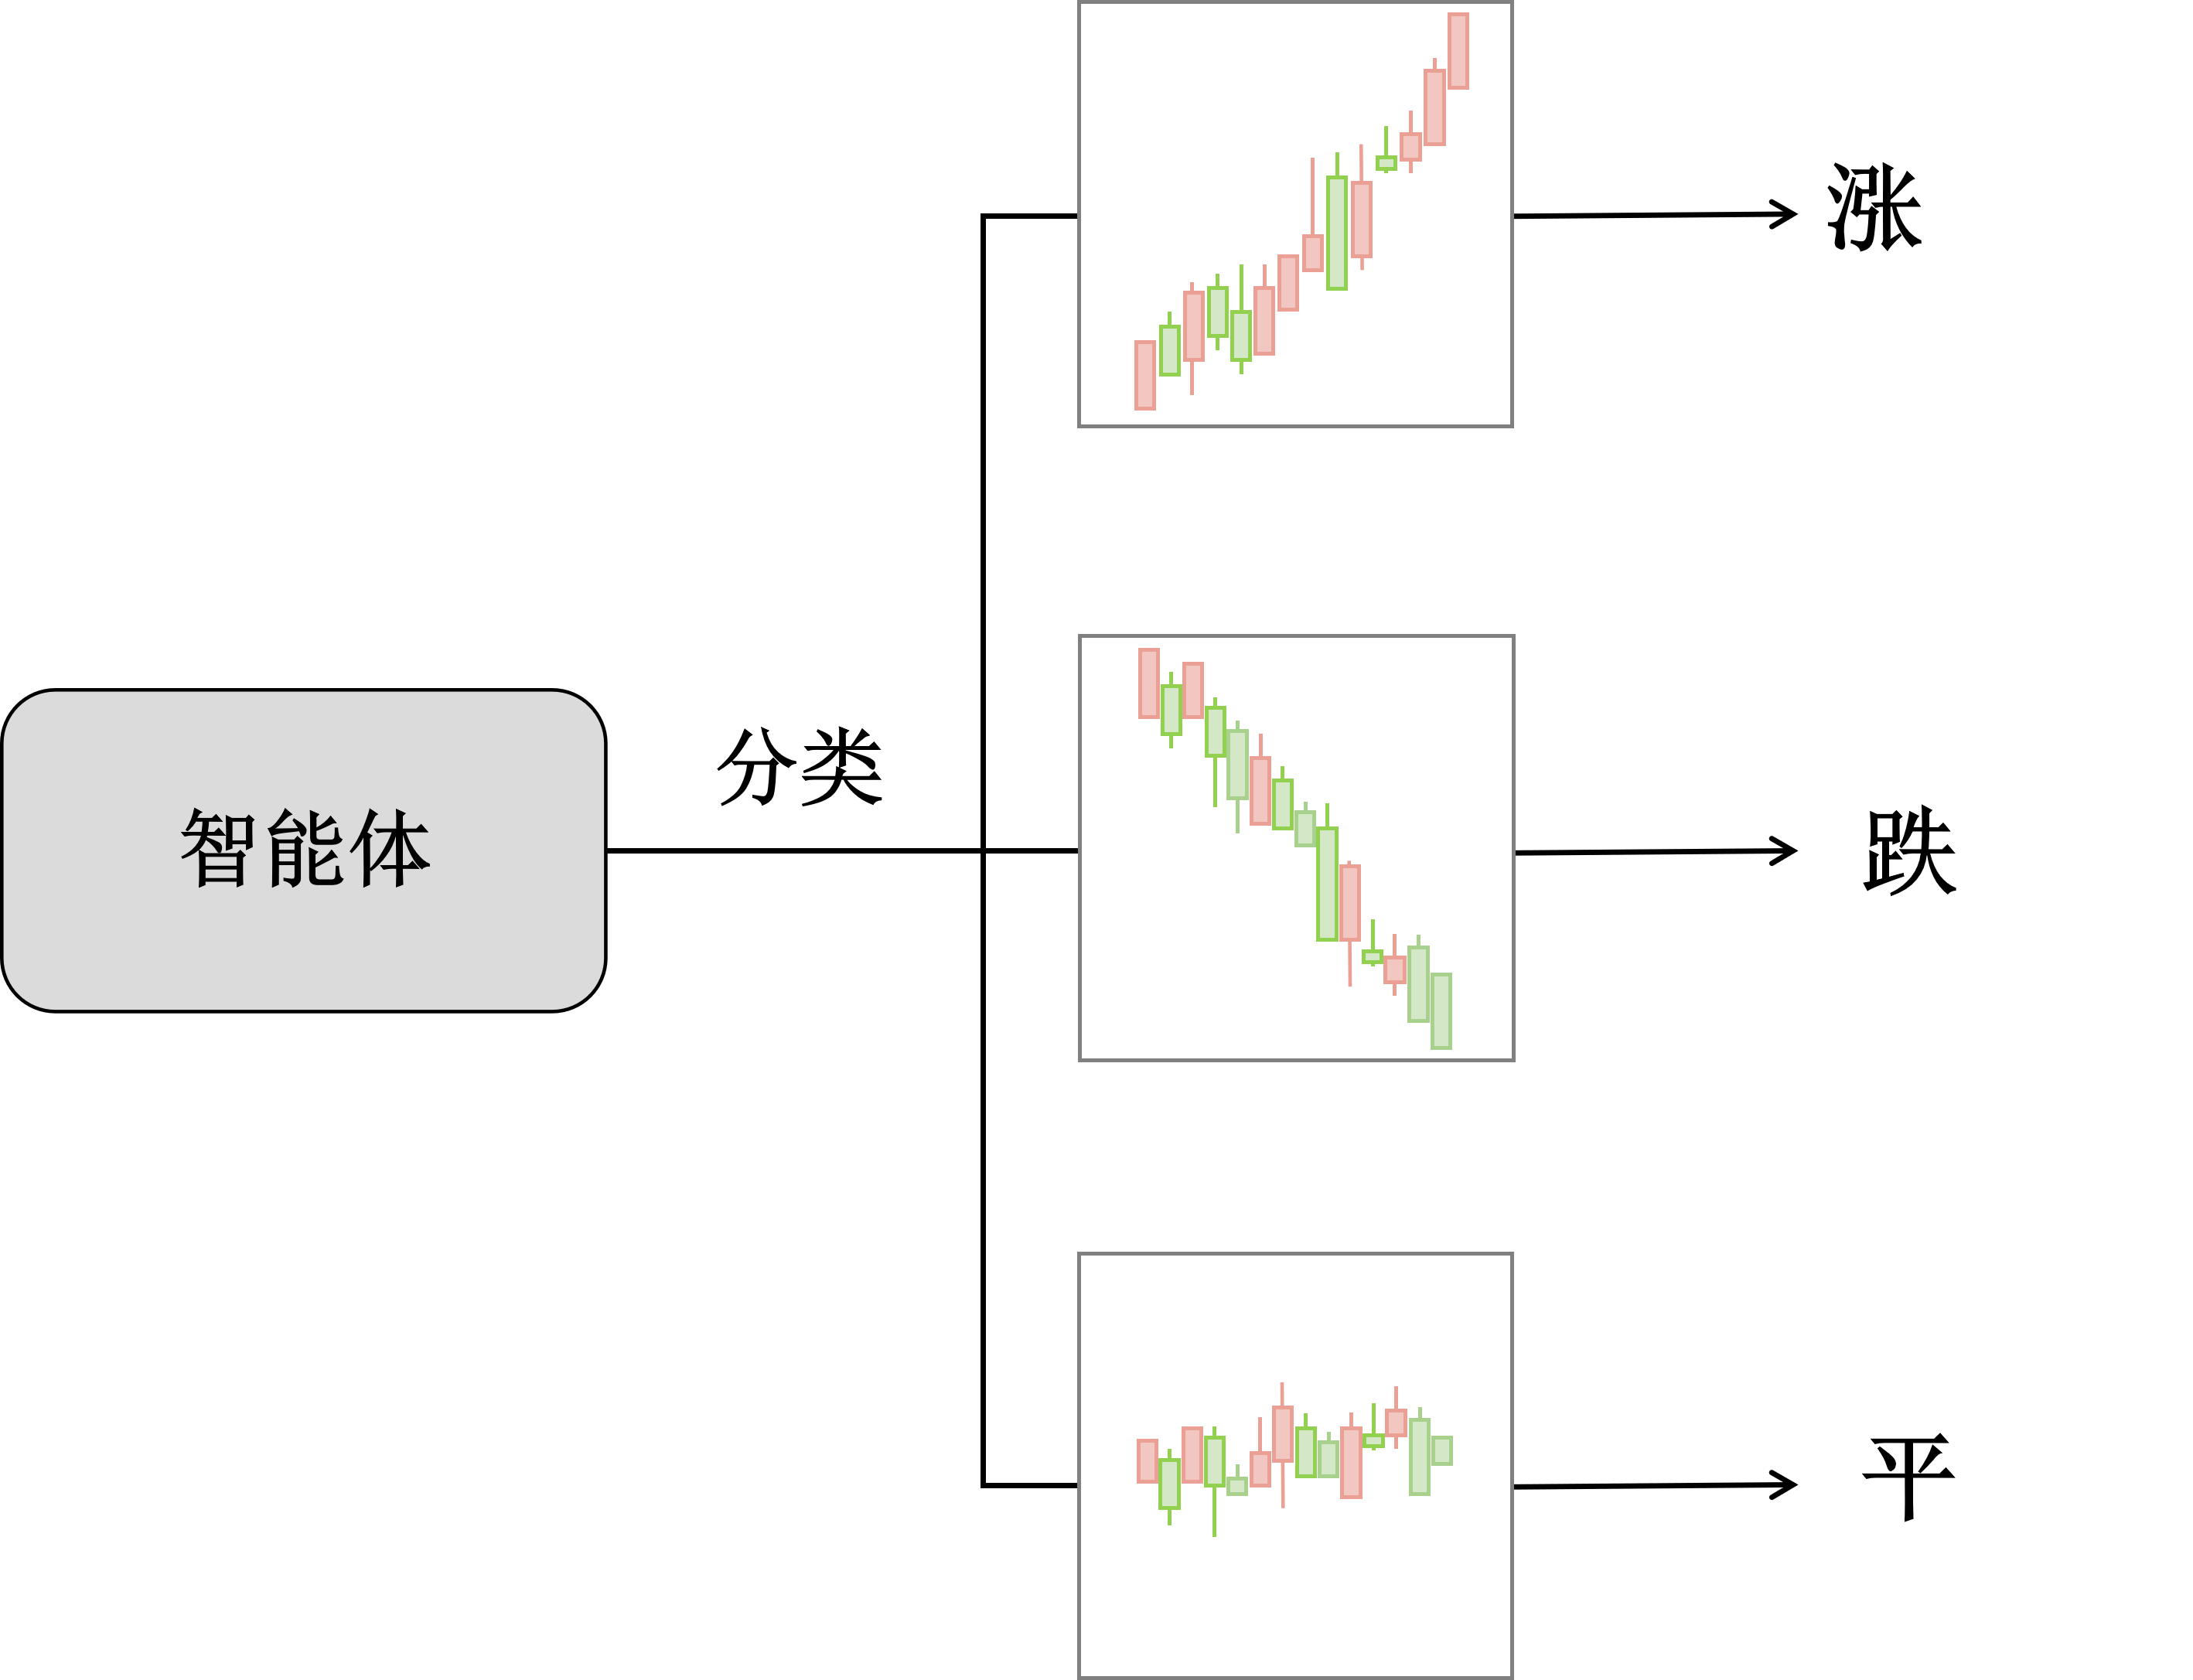
\includegraphics[width=0.5\textwidth]{figures/chap7/偏序/分类任务.png}
\caption{策略整合中的方向输出任务图}
\label{fig:twinclasstaskfig}
\end{figure}

如图\ref{fig:twinclasstaskfig}所示，不同于传统生成对抗网络判别器仅输出单一的真假标量，我们的判别器输出层包含两个关键分支：分类头输出一个3维的逻辑输出向量，对应未来价格的“涨、跌、平”三种趋势的概率分布，这使得判别器输出能够对应最终交易决策中的买入、卖出或持有判断；特征头直接输出倒数第二层的高维特征向量，为GCA和逆向师生蒸馏机制阶段的特征级蒸馏提供了必要的载体，使得落后模型能够直接学习最优模型的内部表征。
架构的关键在于“1个生成器组 × 1个成员、2个判别器组 × 每组3个成员”的非对称配置。预训练后的单个自注意力序列模型生成器持续提供虚拟样本；两个判别器组中的6个异构判别器交替采用卷积神经网络与自注意力序列模型结构。
在损失函数设计上，本文采用兼顾生成质量、分类精度与知识迁移的复合损失体系。

\textbf{（1）生成器金融感知重构损失。}生成器的核心损失函数为金融感知重构损失，该损失对开盘价、最高价、最低价与收盘价价格维度与成交量维度采用不同的损失函数，以适应金融数据的异质性特征。价格维度采用Huber损失，其在误差较小时等价于均方误差以保证平滑梯度，在误差较大时退化为线性损失以抑制价格跳变带来的梯度爆炸；成交量维度采用对数双曲余弦损失，其对零值和异常值具有天然的鲁棒性。两者通过权重系数加权求和：

\begin{equation}
\mathcal{L}_{G}^{\text{recon}} = w_p \cdot \text{Huber}_{\delta=1.0}(\hat{P}_{\text{开高低收}}, P_{\text{开高低收}}) + w_v \cdot \text{对数双曲余弦}(\hat{V}, V)
\label{eq:financial_aware_loss}
\end{equation}
其中$w_p=1.0$，$w_v=0.8$。
\begin{equation}
\text{Huber}_\delta(e) = \begin{cases} \frac{1}{2}e^2, & |e| \leq \delta \\ \delta\left(|e| - \frac{1}{2}\delta\right), & |e| > \delta \end{cases}
\end{equation}
\begin{equation}
\text{对数双曲余弦}(\hat{V}, V) = \frac{1}{N}\sum_{i=1}^{N}\log\left(\cosh(\hat{V}_i - V_i)\right)
\end{equation}

该设计突出价格信息的重要性，同时兼顾成交量这一辅助变量。

\textbf{（2）判别器分类损失。}判别器的损失函数采用基于三分类标签（涨/跌/平）的交叉熵损失：

\begin{equation}
\mathcal{L}_{D}^{\text{交叉熵}} = -\frac{1}{N}\sum_{i=1}^{N}\sum_{c=1}^{3} y_{i,c} \log(\hat{y}_{i,c})
\label{eq:disc_ce_loss}
\end{equation}

其中$c \in \{\text{涨}, \text{跌}, \text{平}\}$。相较于传统生成对抗网络中的二分类真假判别，这种设计迫使判别器不仅要区分数据的来源，更要将价格趋势逻辑转化为策略整合阶段的方向输出。

\textbf{（3）知识蒸馏损失。}在GCA组内对抗、组间对抗以及逆向师生蒸馏环节中，落后判别器通过最小化与最优判别器在特征层和输出层的均方误差实现知识迁移。知识蒸馏最初用于教师模型向学生模型传递软标签信息\cite{hinton2015distilling}。与单向蒸馏不同，深度互学习研究表明，多模型之间可以通过双向学习提升整体表示质量\cite{zhang2018deep}。后续蒸馏综述也表明，蒸馏机制不仅可用于模型压缩，也可用于表示对齐与训练稳定化\cite{huang2022distillation}：

\begin{equation}
\mathcal{L}_{\text{Distill}} = \lambda \cdot \left[\text{均方误差}(\mathbf{f}_i, \mathbf{f}^*) + \text{均方误差}(\mathbf{z}_i, \mathbf{z}^*)\right]
\label{eq:distill_loss}
\end{equation}

其中$\mathbf{f}_i$和$\mathbf{f}^*$分别为当前判别器和最优判别器倒数第二层的特征表示，$\mathbf{z}_i$和$\mathbf{z}^*$为对应的输出层逻辑输出，蒸馏权重系数$\lambda=0.1$。这一设计在保持判别器多样性的同时引导其向最优解收敛。与静态平均集成不同，蒸馏项在训练过程中直接约束中间表征和输出分布，因而更适合用于多判别器间的动态知识协调。

\textbf{（4）赛马场学生蒸馏损失。}在赛马场竞争阶段，新初始化的学生判别器通过拟合所有现有判别器的集成输出实现快速知识吸收：

\begin{equation}
\mathcal{L}_{\text{Student}} = \mathcal{L}_D^{\text{交叉熵}} + \lambda \cdot \text{均方误差}\left(\mathbf{z}_{\text{student}},\; \frac{1}{K}\sum_{k=1}^{K}\mathbf{z}_k\right)
\label{eq:rt_student_loss}
\end{equation}

其中$K$为所有判别器的总数，$\mathbf{z}_k$为第$k$个判别器的输出，$\lambda=0.1$。

\textbf{（5）生成对抗网络微调损失。}在孪生对抗自体再生阶段的最终微调中，生成器与判别器的损失函数分别为：
\begin{equation}
\mathcal{L}_{G}^{\text{finetune}} = \mathcal{L}_{G}^{\text{recon}} + 0.1 \times \mathcal{L}_{D}^{\text{交叉熵}}(D_{\text{best}}(G(\mathbf{x})), \mathbf{y})
\label{eq:gan_finetune_g}
\end{equation}
\begin{equation}
\mathcal{L}_{D}^{\text{finetune}} = \mathcal{L}_{D}^{\text{交叉熵}}(D_{\text{best}}(\mathbf{x}), \mathbf{y})
\label{eq:gan_finetune_d}
\end{equation}

生成器损失同时约束重构质量与对抗能力，判别器损失则聚焦最终分类精度。


\subsection{偏序协同对抗的理论基础与层级博弈假设}

本节将偏序协同对抗（PCA）界定为策略整合阶段的组织框架，而不是全文的第二个基础架构。其核心作用在于规定资产配置、因子表征、时序结构信号和执行约束进入最终交易决策之前的整合顺序，使涨、跌、平分类结果能够作为策略整合后的输出，而不是脱离交易流程的孤立标签。

从方向信号生成看，PCA需要同时处理局部形态与长程依赖，但二者不应被简单视为并列特征分支。局部结构更适合刻画盘口形态、短周期波动和局部价格变化模式，限价指令簿深度学习模型也表明，卷积结构能够用于捕捉盘口局部空间结构，并与时序模块共同学习价格运动依赖\cite{zhang2019DeepLOB}。因此，在本章框架中，卷积判别器主要承担局部结构识别功能，其输出为后续方向判断提供基础证据。

在更长时间跨度上，交易信号还受到跨时段依赖、状态切换和历史信息传递的影响。自注意力机制为长序列依赖建模提供了基础\cite{vaswani2017attention}，因此，本章引入自注意力判别器，用于补充卷积判别器对局部形态的刻画不足。二者并非简单叠加，而是在偏序协同框架下形成“局部形态识别—长程依赖校正—策略输出整合”的层级关系。

PCA的理论基础并不在于再次扩展架构概念，而在于将不同类型的判别信息按照偏序顺序进入策略整合流程。局部形态首先提供方向识别的初始依据，长程依赖进一步修正短期信号可能带来的误判，最终分类结果再与买入、卖出、持有判断、仓位映射和跨资产泛化检验相衔接。由此，PCA强调的是策略整合阶段的组织顺序和层级约束，而不是多个预测模型的并列堆叠。

\subsection{架构的设计与多空博弈建模}

本节的“架构设计”仅指第六章内部用于策略整合的多空博弈组织方式，不再承担全文基础架构功能。传统生成对抗网络通过生成器与判别器之间的对抗学习数据分布\cite{goodfellow2014generative}，但直接用于涨跌分类时，单一判别器容易只对少数局部模式形成反馈。时间序列生成对抗网络说明，对抗生成可以与时序监督信息结合\cite{yoon2019time}。据此，本章保留生成器作为样本边界扰动源，但最终策略信号由判别器组在偏序约束下共同形成。

在判别器侧，多组多成员结构用于提供多源反馈。多生成器多判别器研究表明，多个判别器能够从不同角度评估生成样本\cite{durugkar2017generative}；专业化判别器方法也说明，不同判别器关注不同子分布，有助于提高复杂分布下的覆盖能力\cite{choi2022mclgan}。
对应到本章，卷积神经网络判别器偏向局部形态和短周期价格变化模式，高频方向预测研究也表明，卷积结构能够从价格序列中提取短周期方向特征\cite{tsantekidis2017forecasting}。因此，该类判别器主要为多空方向判断提供局部形态依据。
自注意力序列模型判别器则偏向跨变量、跨时间关系建模，多变量时间序列表征学习研究也说明，自注意力结构能够处理复杂时间依赖关系\cite{zerveas2021transformer}。两类判别器在偏序协同框架中并非并列堆叠，而是共同服务于局部信号识别、长程依赖校正和最终策略输出。
逆向师生蒸馏机制在该框架中承担策略信号校正功能。当弱模型在局部市场结构上捕捉到强模型忽视的信息时，系统允许其反向影响较优成员，以降低强模型对局部伪结构的过度自信。由此，本节所谓“架构”不是第二章意义上的基础架构，而是为买入、卖出、持有判断以及策略整合过程组织多空博弈关系。

\subsection{模型架构在极端行情下的适应性优化机制}


孪生对抗自体再生机制在PCA中承担稳定器作用。对第六章而言，极端行情适应性不只是分类器鲁棒性问题，还关系到方向信号能否稳定映射为交易动作：若某一判别器在剧烈波动阶段形成错误方向，后续多空仓位和风险控制都会受到放大影响。本节关注的重点不是单一模型在极端行情下的预测精度，而是策略整合流程在异常波动、模型偏离和信号冲突时是否具备恢复能力。为此，该阶段统计各判别器相对最优判别器的超阈值次数，当异常频次达到 $twins\_threshold$ 且系统中仍存在正常判别器组时，触发替换与微调。

整体训练遵循“GCA基础训练—赛马场竞争—逆向师生蒸馏—孪生自体再生”的偏序顺序。该顺序将分类信号、模型置信度、执行约束和异常修复状态逐步转化为可执行的多空方向，避免多个目标同时进入训练过程而造成震荡。

\begin{algorithm}[H]
\caption{PCA框架总体训练流程}
\label{alg:mgca}
\begin{algorithmic}[0]
\Require 数据集 $\mathcal{D}$（训练集/验证集/测试集），生成器组 $\mathcal{G}$（1组，1个成员），判别器组 $\mathcal{D}_{\text{groups}}$（2组，每组3个成员）
\Ensure 训练好的生成器 $\mathcal{G}_{\text{trained}}$，最优判别器 $\mathcal{D}_{\text{best}}$
\Statex
\State \textbf{/* 初始化 */}
\State 使用随机权重初始化 $\mathcal{G}$ 和 $\mathcal{D}_{\text{groups}}$
\State 配置优化器：$\text{Opt}_{\mathcal{G}}$（学习率=$4\times10^{-5}$），$\text{Opt}_{\mathcal{D}}$（学习率=$2\times10^{-5}$）
\Statex
\State \textbf{/* 偏序协同架构基本训练：群组交叉对抗（GCA） */}
\State $\mathcal{G}_{\text{trained}}, \mathcal{D}_{\text{global-best}} \gets \text{Execute-GCA}(\mathcal{G}, \mathcal{D}_{\text{groups}}, \mathcal{D})$
\Statex
\State \textbf{/* 阶段二：赛马场竞争机制 */}
\If{启用赛马场竞争机制}
  \State $\mathcal{D}_{\text{global-best}} \gets \text{Execute-赛马场竞争机制}(\mathcal{G}_{\text{trained}}, \mathcal{D}_{\text{groups}}, \mathcal{D}_{\text{global-best}})$
\EndIf
\Statex
\State \textbf{/* 阶段三：逆向师生蒸馏机制 */}
\If{启用逆向师生蒸馏机制}
  \State $\mathcal{D}_{\text{global-best}} \gets \text{Execute-逆向师生蒸馏机制}(\mathcal{D}_{\text{groups}}, \mathcal{D}_{\text{global-best}})$
\EndIf
\Statex
\State \textbf{/* 阶段四：孪生对抗自体再生机制 */}
\If{启用孪生对抗自体再生机制}
  \State $\mathcal{G}_{\text{trained}}, \mathcal{D}_{\text{best}} \gets \text{Execute-孪生对抗自体再生机制}(\mathcal{G}_{\text{trained}}, \mathcal{D}_{\text{groups}}, \mathcal{D}_{\text{global-best}})$
\Else
  \State $\mathcal{D}_{\text{best}} \gets \mathcal{D}_{\text{global-best}}$
\EndIf
\Statex
\State \Return $\mathcal{G}_{\text{trained}}, \mathcal{D}_{\text{best}}$
\end{algorithmic}
\end{algorithm}

% 

GCA 阶段的核心在于通过组内与组间两层蒸馏实现优胜劣汰。生成器先在金融感知损失约束下预训练，再生成虚拟数据构造混合样本；随后各判别器先向组内最优者对齐，再由各组代表向全局最优者对齐，从而推动系统由局部最优逐步收敛至更优解。

\begin{algorithm}[H]
\caption{偏序协同架构基本训练 - 群组交叉对抗（GCA）}
\label{alg:gca}
\begin{algorithmic}[0]
\State \textbf{阶段1：生成器预训练}
\For{epoch $\in$ Init\_Epochs}
  \State $\text{损失}_G = \text{金融\_Aware\_Loss}(G(x), \text{real\_x})$
  \State 使用 $\text{损失}_G$ 更新生成器 $G$
\EndFor
\State 上述步骤训练完成后得到训练好的生成器$\mathcal{G}_{\text{trained}}$
\Statex
\State \textbf{阶段2：混合数据生成}
\State $\text{Data\_Mixed} = \text{Mix}(\text{Real\_Data},\; \mathcal{G}_{\text{trained}}(x),\; \text{ratio}=1-\text{fake\_ratio})$
\Statex
\State \textbf{阶段3：组内对抗}
\For{$D_{\text{groups}}$ 中的每个组}
  \State 在 $\text{Data\_Mixed}$ 上训练组内所有判别器
  \State 在验证集上评估，选出组内最优 $\text{Group\_Best}$（交叉熵最小）
  \For{组内每个判别器}
    \If{该判别器 $\neq$ $\text{Group\_Best}$}
      \State $\text{损失}_{\text{Distill}} = \text{均方误差}(\text{Feat}, \text{Group\_Best.特征}) + \text{均方误差}(\text{逻辑输出}, \text{Group\_Best.逻辑输出})$
      \State 使用 $\text{损失}_{\text{Distill}}$ 更新该判别器
    \EndIf
  \EndFor
\EndFor
\Statex
\State \textbf{阶段4：组间对抗}
\State 从所有 $\text{Group\_Best}$ 中选出全局最优 $\text{Global\_Best}$
\For{每个 $\text{Group\_Best}$}
  \If{$\text{Group\_Best} \neq \text{Global\_Best}$}
    \State $\text{损失}_{\text{Distill}} = \text{均方误差}(\text{Feat}, \text{Global\_Best.特征}) + \text{均方误差}(\text{逻辑输出}, \text{Global\_Best.逻辑输出})$
    \State 使用 $\text{损失}_{\text{Distill}}$ 更新 $\text{Group\_Best}$
  \EndIf
\EndFor
\end{algorithmic}
\end{algorithm}

如算法\ref{alg:gca}及图\ref{fig:GCA-Partial-GCA}所示，群组交叉对抗（GCA）阶段通过将判别器分组并引入组间特征蒸馏，使得落后判别器能够快速学习全局最优判别器的特征表示，从而在保持组内多样性的同时提升整体判别能力。
在PCA流程中，“生成器”与GCA相似，实际上充当的是“预测模型”的角色。将其称为“生成器”
同样是为了将其纳入“对抗学习”的框架中，但其本质任务依然是条件预测。赛马场竞争机制承担动态筛选与模型更新作用。该阶段通过引入新学生判别器与末位替换，使判别器组在保持多样性的同时更新低效成员。
逆向师生蒸馏机制阶段用于校正判别器之间的边界差异。系统动态比较“学生”（当前较弱判别器）与“教师”（其他判别器）的性能差距，并根据局部样本上的相对表现选择正向蒸馏或反向反馈。


\begin{figure}[htbp]
  \centering
  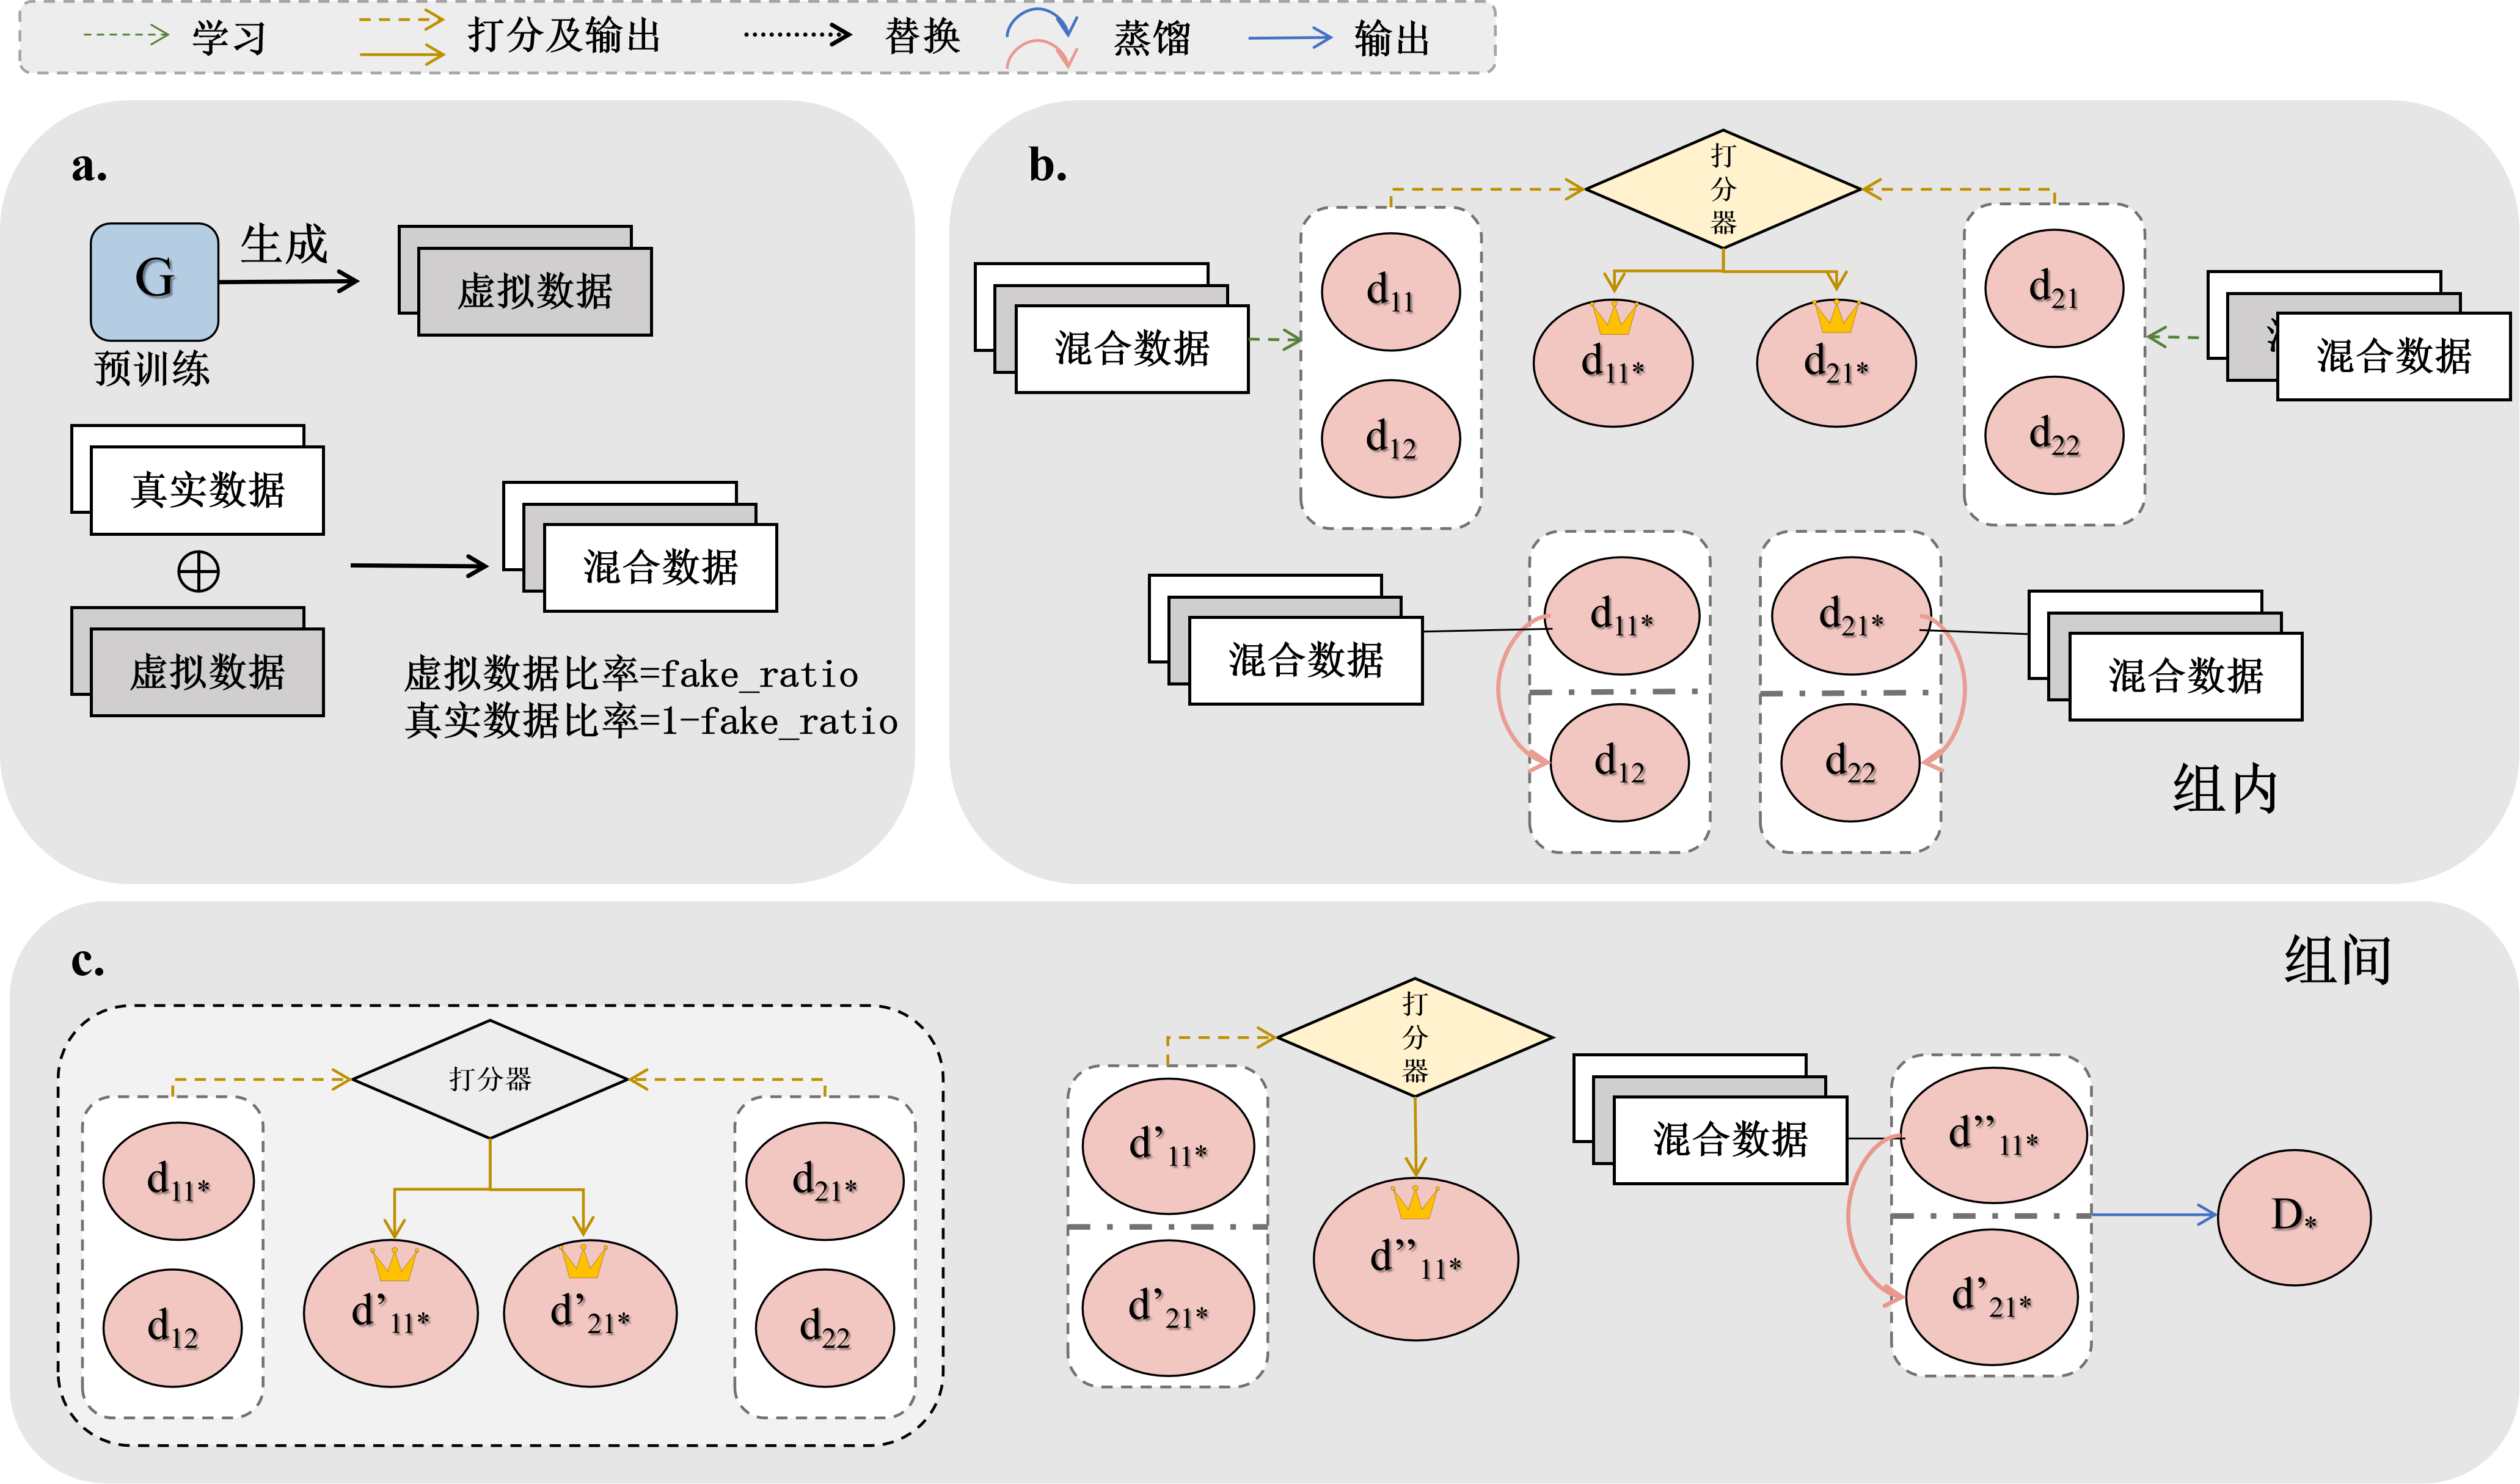
\includegraphics[width=0.8\textwidth]{figures/chap7/偏序/群组偏序.png}
  \caption{偏序协同对抗机制下的群组交叉对抗训练流程示意图}
  \label{fig:GCA-Partial-GCA}
\end{figure}

% 
    


\begin{algorithm}[H]
\caption{赛马场竞争机制算法流程}
\label{alg:racetrack}
\begin{algorithmic}[0]
\State \textbf{阶段1\&2：评估与定位}
\State 评估所有判别器，找到全局最差 $\texttt{Global\_Worst}$ 和全局最优 $\texttt{Global\_Best}$
\Statex
\State \textbf{阶段3：训练新学生}
\State 初始化 $\texttt{Student\_D}$（深拷贝 $\texttt{Global\_Best}$）
\For{$\texttt{Mixed\_Data}$ 中的每个批次}
  \State $\texttt{Teacher\_Ensemble} \gets \text{Average}(\text{All\_Discriminators}(\text{batch}))$
  \State $\text{损失\_Student} \gets \text{交叉熵}(\texttt{Student\_D}(\text{batch}), \text{label}) + \lambda \cdot \text{均方误差}(\texttt{Student\_D}(\text{batch}), \texttt{Teacher\_Ensemble})$
  \State 更新 $\texttt{Student\_D}$
\EndFor
\Statex
\State \textbf{阶段4\&5：替换}
\State 使用 $\texttt{Student\_D}$ 替换 $\texttt{Global\_Worst}$
\State 重置被替换位置的优化器
\State 重新评估并更新 $\texttt{Global\_Best}$
\end{algorithmic}
\end{algorithm}

% 



\begin{algorithm}[H]
\caption{逆向师生蒸馏机制算法流程}
\label{alg:s2t}
\begin{algorithmic}[0]
\State \textbf{阶段1：初始打分}
\State 使用打分器（验证集交叉熵）评估每个判别器组的每个判别器
\State 找到全局交叉熵最小的判别器 $a_1$ 和全局交叉熵最大的判别器 $b_1$
\Statex
\State \textbf{阶段2：混合数据训练}
\State 所有判别器组中的所有判别器在赛马场阶段生成的混合数据上进行训练
\Statex
\State \textbf{阶段3：单向蒸馏}
\State 使用打分器重新评估，找到新的全局最优 $a_2$ 和全局最差 $b_2$
\For{每个判别器 $D_i$（$D_i \neq a_2$）}
  \State $\text{损失}_{\text{Distill}} = \text{均方误差}(\text{Feat}_{D_i}, \text{Feat}_{a_2}) + \text{均方误差}(\text{逻辑输出}_{D_i}, \text{逻辑输出}_{a_2})$
  \State 使用 $\text{损失}_{\text{Distill}}$ 更新 $D_i$，使其特征分布向 $a_2$ 靠拢
\EndFor
\Statex
\State \textbf{阶段4：组内循环评分与双向反馈}
\State 将 $b_1$ 位置的判别器定义为“学生”，其余所有判别器定义为“教师”，初始化阈值$\theta$
\For{每个教师判别器 $T_j$}
  \If{学生交叉熵 + $\theta$ < 教师交叉熵（学生超越教师）}
    \State 反向蒸馏：引导教师 $T_j$ 对齐学生在局部样本上的有效输出与特征
  \ElsIf{教师交叉熵 + $\theta$ < 学生交叉熵（学生落后于教师）}
    \State 正向蒸馏：引导学生对齐教师 $T_j$ 的输出与特征
  \EndIf
\EndFor
\Statex
\State \textbf{阶段5：最终评估}
\State 使用打分器评估所有判别器，找到交叉熵最小的全局最优判别器并输出
\end{algorithmic}
\end{algorithm}

如算法\ref{alg:s2t}及图\ref{fig:GCA-Partial-S2T}所示，逆向师生蒸馏机制阶段建立了一种双向反馈机制。当学生判别器在特定数据分布上表现优于教师判别器时，系统触发反向蒸馏，使教师模型对学生模型在局部样本中的有效响应进行对齐，从而缓解传统单向蒸馏中信息流动不足的问题。
最后，孪生对抗自体再生机制阶段承担稳定修复作用。算法统计逆向师生蒸馏机制阶段中每个判别器相对最优判别器的偏离程度。

\begin{figure}[htbp]
  \centering
  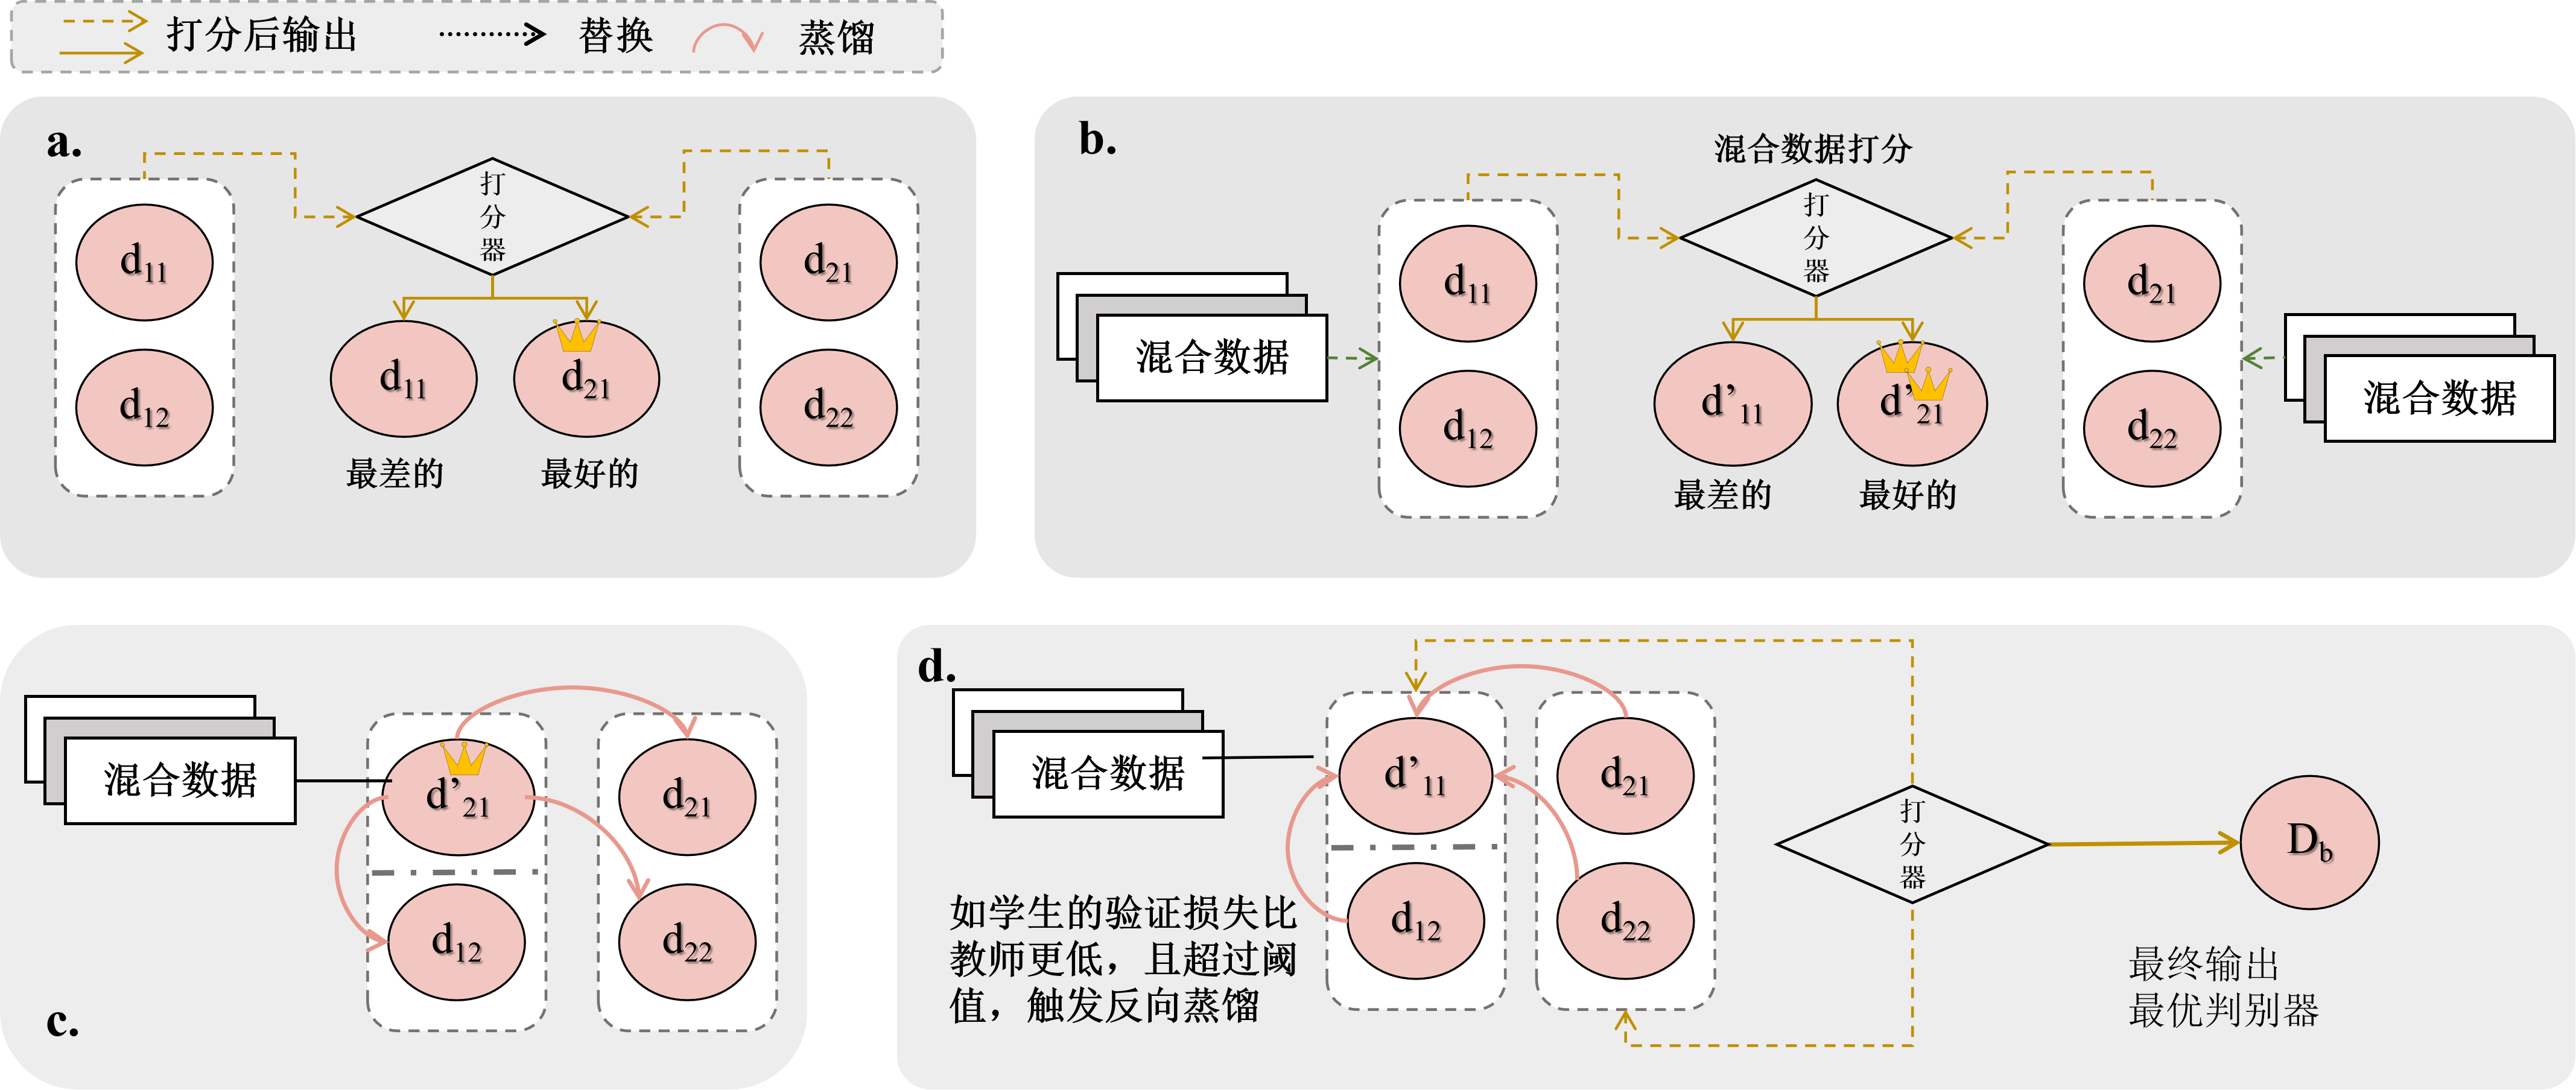
\includegraphics[width=0.8\textwidth]{figures/chap7/偏序/逆向教师偏序.png}
  \caption{偏序协同对抗机制下的逆向师生蒸馏机制训练流程示意图}
  \label{fig:GCA-Partial-S2T}
\end{figure}

% 



\begin{algorithm}[H]
\caption{孪生对抗自体再生机制算法流程}
\label{alg:twin_adversarial_detection}
\begin{algorithmic}[0]
\State \textbf{异常检测}
\State 统计每个判别器相对于 \textit{Global\_Best} 的超阈值次数 \textit{exceed\_threshold\_times}
\State \textbf{条件1：}超阈值次数 $\geq$ \textit{twins\_threshold}
\State \textbf{条件2：}至少有另一个判别器组状态正常
\Statex
\State \textbf{替换与微调}
\For{每个判别器}
  \If{同时满足条件1和条件2}
    \State 使用 \textsc{DeepCopy}(\textit{Global\_Best}) 替换该判别器
    \State 重置优化器
  \EndIf
\EndFor
\Statex
\State \textbf{生成对抗网络微调}
\For{epoch $\in$ \textit{Finetune\_Epochs}}
  \State 训练 $G$：$\mathcal{L}_G = \text{金融\_Loss} + 0.1 \times \text{Adversarial\_Loss}(D_{\text{best}})$
  \State 训练 $D_{\text{best}}$：$\mathcal{L}_D = \text{交叉熵\_Loss}$
\EndFor
\end{algorithmic}
\end{algorithm}

% 

设生成器数为 $N_G$（本文取1），判别器数为 $N_D$（本文取6），时间步长为 $T$，特征维度为 $F$。单轮训练中，生成器复杂度约为 $\mathcal{O}(N_G \cdot T^2 \cdot F)$，判别器前向传播复杂度为 $\mathcal{O}(N_D \cdot C_D)$；GCA 与逆向师生蒸馏机制中的特征对齐额外引入 $\mathcal{O}(N_D^2 \cdot d_{feat})$ 开销。

\subsection{多智能体偏序协同对抗整体框架与策略融合路径}

综合前述设计，PCA在第六章中的核心作用是完成策略整合，而不是重新建立独立基础架构。本节所说的“策略整合路径”，是指第六章内部将方向信号、模型置信度、训练约束和异常修复状态组织成最终交易判断的过程。第2章侧重资金配置，第3章侧重配置依据形成，第4章侧重交易时机判断，第5章侧重交易动作落地；本章则把方向分类组织为买入、卖出或持有的输出接口。

该路径包括三层含义。第一是信号层：生成器与判别器在真实样本和生成样本共同构成的环境中学习方向边界。第二是约束层：赛马场竞争、逆向师生蒸馏与孪生对抗自体再生按顺序进入训练，分别承担筛选、校正和修复功能。第三是决策层：判别器输出概率、模型置信度、执行约束与异常修复状态共同影响买入、卖出或持有判断。经过这一处理，PCA不只是展示模型架构，而是说明方向信号如何进入最终交易决策。

\section{实验}

本章实验面向策略整合任务，检验偏序协同对抗学习方法在不同期货合约与不同市场状态下的表现。实验不把分类准确率作为唯一目标，而是结合判别器性能、交易收益、夏普比率、胜率和跨资产稳定性，判断涨、跌、平输出是否能够支撑买入、卖出或持有决策。这里验证的是PCA在最终交易判断环节中的组织能力，而不是重新证明前述各章方法的全部有效性。

\subsection{实验数据集}

本节检验偏序协同对抗学习方法在策略整合任务中的表现。实验中的涨、跌、平分类信号被视为最终交易决策的输出形式，其质量不仅通过分类指标衡量，还需要结合交易映射、跨资产稳定性和收益风险表现分析。下文先介绍实验设计与评估体系，再分析数据集特征、模型分类性能、交易映射表现及各机制对策略整合过程的贡献。

本章实验逻辑延续了前文的评价体系，并在更复杂的策略整合任务下验证了前述偏序结构的普适性。
由于金融样本具有时间依赖与标签重叠特征，实验评估不能采用普通随机切分方式。金融机器学习方法论强调，样本外验证应尽量避免信息泄漏，并通过 purging、embargo 等手段降低训练集与测试集之间的标签污染风险\cite{lopezdeprado2018advances}。同时，回测过拟合研究也指出，若在同一历史样本上反复筛选模型和参数，表观绩效可能被系统性高估\cite{bailey2015pbo}。因此，本章在实验解释中同时关注分类指标、交易指标和跨资产稳定性，而不是仅依据单一准确率判断模型优劣。
实验基于深度学习框架完成。生成器与判别器均采用自适应矩估计优化器，学习率分别设为 $4\times10^{-5}$ 和 $2\times10^{-5}$，动量参数为 $(0.9, 0.999)$，批量大小为64，初始训练轮数为100。

\begin{figure}[h]
\centering
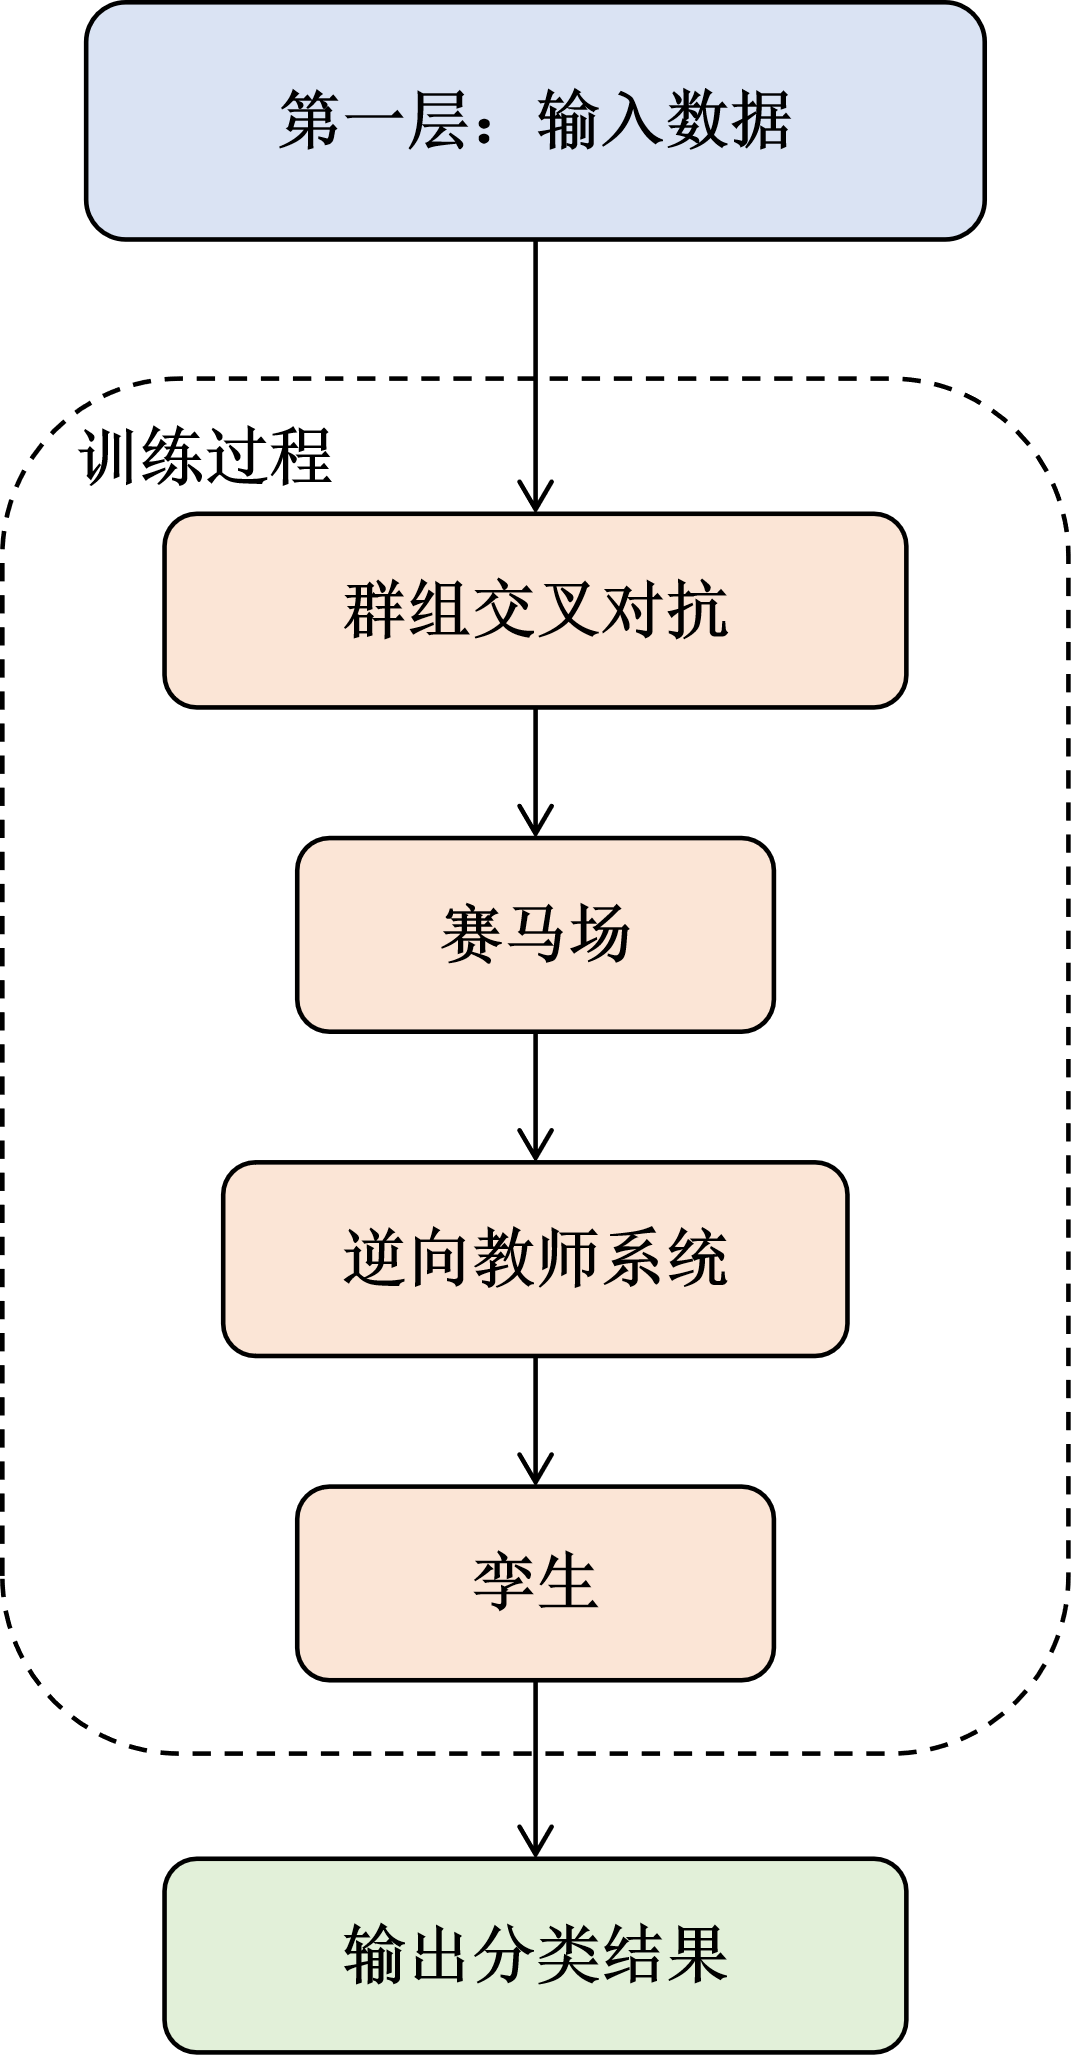
\includegraphics[width=0.5\textwidth]{figures/chap7/偏序/偏序架构.png}
\caption{偏序协同对抗架构图}
\label{fig:Partialorderadversarialarchitecture}
\end{figure}

如图\ref{fig:Partialorderadversarialarchitecture}所示，偏序协同对抗架构（PCA）通过上述四个阶段的有机结合，构成了PCA策略整合流程中的训练底座。为评估该框架的性能，本章构建了涵盖价格预测精度、判别器分类能力、成交量预测质量与交易表现的综合评估指标体系。
本章的交易回测以判别器输出的涨跌分类信号为基础，通过预设的信号生成规则将分类预测转换为交易指令（买入、卖出、持有），并以每笔交易的单期收益率作为核心绩效衡量指标。
具体而言，回测过程不引入保证金制度或账户复利，仅统计每笔完整交易的价格变化率。\begin{equation}
r_{\text{trade}} = \frac{P_{\text{exit}} - P_{\text{entry}}}{P_{\text{entry}}}.
\end{equation}
基于 $N$ 笔交易的收益率序列 $\{r_1, r_2, \dots, r_N\}$，各评估指标计算方式如下：
\begin{itemize}
  \item \textbf{平均收益率} $\bar r = \frac{1}{N}\sum_{i=1}^{N} r_i$：所有交易笔收益率的算术平均值，反映策略的单笔平均盈利能力。该指标为原始比例（非百分比），不代表年化复利收益。
  \item \textbf{胜率} $\text{胜率} = \frac{\#\{r_i > 0\}}{N}$：盈利交易笔数占总交易笔数的比例。
  \item \textbf{夏普比率} $\text{夏普比率} = \frac{\bar r}{\sigma_r} \cdot \sqrt{252}$：其中 $\sigma_r$ 为交易收益率的标准差，$\sqrt{252}$ 为年化因子（隐含日频交易假设）。当交易笔数少于 2 或 $\sigma_r$ 过小时，夏普比率设为 0。
\end{itemize}

需要说明的是，文中“年化收益率”仅为 $\bar r \times 252$ 的参照表达，并非账户实际复利收益。
实验涵盖19个中国期货合约，覆盖股指、贵金属、基础金属、能源、农产品等类别，所有实验均在生成器学习率 $4\times10^{-5}$ 的统一设置下进行。为保证统计可靠性，交易性能分析仅保留交易次数不少于5笔的配置。
在多配置对比中，模型选择本身也可能引入数据窥探偏差。真实性检验和优越预测能力检验分别从多模型检验与优越预测能力角度讨论了这种风险\cite{white2000realitycheck,hansen2005spa}。本文并不把这些检验直接作为统计显著性证明，而是借鉴其问题意识，在结果分析中同时报告多配置、多合约和多资产类别下的表现，避免只展示少数最优案例。
PCA采用模块化设计，偏序协同架构为基础配置，赛马场竞争机制、逆向师生蒸馏机制与孪生对抗自体再生机制可灵活组合。配置代码中，第一位表示是否启用偏序协同架构，后两位分别表示赛马场竞争机制和逆向师生蒸馏机制；基线模型则为不含偏序协同架构的传统单生成器单判别器模式。
实验平台配备英伟达 GeForce RTX 3090 图形处理器、Intel Core i9-10900K 中央处理器和 64GB 内存，软件环境采用 Ubuntu 系统与深度学习框架，数据处理主要依赖常用科学计算与机器学习工具库。
考虑到生成对抗网络训练的敏感性，实验统一设置全局随机种子，采用 Xavier均匀初始化，并通过可视化工具监控损失曲线、梯度范数和验证集均方误差。训练中使用早停机制：若验证集均方误差连续10个 epoch 未下降，则终止训练并回滚到最优权重，同时定期保存中间检查点以支持后续分析。

为理解PCA策略整合流程的性能表现，本节首先分析19个期货合约的原始数据特征和市场特征。每个合约包含830个每日数据点，涉及7大资产类别，展现出不同的市场特征。

\begin{table}[H]
\centering
\caption{资产类别统计特征}
\label{tab:assetstatssideways}
\footnotesize
\setlength{\tabcolsep}{4pt}
\renewcommand{\arraystretch}{1.18}
\begin{tabular}{lccccccc}
\toprule
\textbf{资产类别} & \textbf{合约数} & \textbf{数据点数} & \makecell{\textbf{平均收益率}\\\textbf{(\%)}} & \makecell{\textbf{收益率}\\\textbf{标准差(\%)}} & \textbf{收益率范围} & \textbf{平均偏度} & \textbf{平均峰度} \\
\midrule
国债 & 1 & 830 & 0.0096 & 0.1704 & $-0.91\%$ 到 $0.67\%$ & -0.62 & 2.86 \\
贵金属 & 2 & 830 & 0.0895 & 1.1572 & $-8.07\%$ 到 $7.35\%$ & -0.31 & 4.12 \\
股指 & 2 & 830 & -0.0194 & 1.2263 & $-10.02\%$ 到 $8.69\%$ & 0.12 & 10.11 \\
基础金属 & 2 & 830 & 0.0113 & 1.7258 & $-17.00\%$ 到 $17.00\%$ & 0.01 & 7.73 \\
能源 & 2 & 830 & 0.0105 & 2.2318 & $-13.18\%$ 到 $25.58\%$ & 1.38 & 16.27 \\
农产品 & 7 & 830 & -0.0151 & 1.4126 & $-17.03\%$ 到 $7.91\%$ & -0.71 & 8.37 \\
工业品 & 3 & 830 & -0.0013 & 1.7733 & $-11.99\%$ 到 $9.53\%$ & -0.12 & 2.53 \\
\bottomrule
\end{tabular}
\end{table}
\begin{table}[H]
\centering
{\small\textbf{续表}}\\[0.5em]
\footnotesize
\setlength{\tabcolsep}{6pt}
\renewcommand{\arraystretch}{1.18}
\begin{tabular}{lp{0.68\textwidth}}
\toprule
\textbf{资产类别} & \textbf{市场特征} \\
\midrule
国债 & 接近零收益、低波动、负偏度 \\
贵金属 & 正收益、中等波动、负偏度 \\
股指 & 负收益、中等波动、高峰度 \\
基础金属 & 正收益、高波动 \\
能源 & 正收益、极高波动、正偏度、高峰度 \\
农产品 & 负收益、中等波动、负偏度 \\
工业品 & 接近零收益、高波动 \\
\bottomrule
\end{tabular}
\end{table}

国债类别以十年债T为代表，展现出金融市场中最稳定的特征，其收益率标准差仅为0.1704\%，是所有资产类别中波动性最低的，收益率分布呈现负偏度特征（-0.62），表明极端下跌事件相对更频繁，但整体波动幅度极小，峰度为2.86接近正态分布，这种低波动性特征使得判别器在该合约上能够更准确地捕捉价格模式。
贵金属类别包含沪金au和沪银ag两个合约，平均收益率为0.0895\%，高于多数资产类别，收益率标准差为1.1572\%，属于中等波动水平，负偏度（-0.31）表明价格下跌时波动相对更大，峰度4.12略高于正态分布，说明存在一定的极端价格波动。
股指类别包含沪深300IF和上证50IH两个合约，平均收益率为负值（-0.0194\%），反映了统计期间股指市场的整体下行趋势；其峰度为10.11，远高于正态分布水平，表明股指市场存在较多极端价格波动。
基础金属类别包含铜cu和镍ni两个合约，平均收益率为正（0.0113\%），收益率标准差达到1.7258\%，属于高波动类别，收益率范围从-17.00\%到17.00\%，展现出基础金属市场的剧烈波动特性，偏度接近零（0.01）表明分布相对对称，峰度7.73说明极端事件较为常见。
能源类别包含原油sc和液化石油气pg两个合约，是所有资产类别中波动性最高的，收益率标准差达到2.2318\%，收益率范围从-13.18\%到25.58\%，特别是液化石油气pg展现出极端的正偏度（2.96）和高峰度（29.21），表明该合约存在罕见的大幅上涨事件，这种高波动性对PCA策略整合流程提出了严峻挑战，但实验结果显示该框架仍然成功实现了从负收益到正收益的转变。
农产品类别包含7个合约（棉花CF、苹果AP、玉米c、豆粕m、豆油y、菜籽油OI、尿素UR），是合约数量最多的类别，平均收益率为负值（-0.0151\%），收益率标准差为1.4126\%属于中等波动，负偏度（-0.71）表明价格下跌时波动更大，峰度8.37说明存在较多的极端价格事件，这种负收益和负偏度特征反映了农产品市场在统计期间的整体疲软。
工业品类别包含3个合约（螺纹钢rb、铁矿石i、对苯二甲酸PTA），平均收益率接近零（-0.0013\%），收益率标准差为1.7733\%属于高波动类别，偏度接近零（-0.12）表明分布相对对称，峰度2.53接近正态分布，这种高波动但分布相对正态的特征使得工业品市场既充满交易机会又保持一定的可预测性。

在完成基础统计后，本节进一步通过可视化手段深入剖析数据特征的分布规律。
国债类别（十年债T）展现出最集中的分布形态，收益率主要集中在-0.5\%到0.5\%的狭窄区间内，标准差仅为0.17\%，反映了国债市场的极低波动性和高度稳定性。贵金属类别（沪金au、沪银ag）呈现中等波动水平，分布较为对称但略带负偏，收益率范围为-8\%到7\%，平均波动率1.16\%。
波动率排名呈现分层结构：最高波动率组由镍ni（2.42\%）、铁矿石i（2.31\%）、原油sc（2.30\%）和液化石油气pg（2.17\%）组成，这四个合约均属于基础金属和能源类别，反映了这些大宗商品市场受全球供需关系、宏观经济和地缘政治因素影响的剧烈波动特性。中等波动率组包括农产品和工业品合约，波动率在1.2\%-1.9\%范围内，如尿素UR(1.92\%）、苹果AP（1.64\%）等。
在深入理解数据集特征的基础上，本小节将核心焦点转向模型性能的评估，首先对比偏序协同架构与传统基线模型在判别器分类任务上的表现差异。
在展开详细分析之前，有必要明确本章涉及的三个关键对比基准的定义及其架构差异：

\begin{itemize}
\item \textbf{基线模型}：传统单模型架构，由1个生成器和1个判别器组成，使用独立的标准对抗训练流程（\texttt{train\_baseline\_model}），不涉及PCA策略整合流程的任何组件。每个合约运行4种基线模型配置：基线-卷积神经网络-直接预测、基线-卷积神经网络-变分自编码器、基线-自注意力序列模型-直接预测、基线-自注意力序列模型-变分自编码器，其中判别器类型（卷积神经网络或自注意力序列模型）由配置名称显式指定，生成器类型从门控循环单元、长短期记忆网络、自注意力序列模型三种架构中选取（具体类型因进程级随机种子而异，实验输出中未记录），成交量预测方法（直接预测或变分自编码器）决定成交量加权平均价格执行时的成交量来源。对比时选取每个合约上表现最优的基线模型配置。
\item \textbf{PCA基础配置-000}：采用单生成器（自注意力序列模型）+单判别器（卷积神经网络）的架构，通过PCA策略整合流程的训练流程（\texttt{train\_single\_experiment}）进行训练，三个机制全部关闭（GCA=0, 赛马场竞争机制=0, 逆向师生蒸馏机制=0）。PCA基础配置-000与基线模型的区别体现在两个层面：（1）模型类型固定——PCA基础配置-000的生成器始终为自注意力序列模型（代码中\texttt{gen\_types[0]}）、判别器始终为卷积神经网络（代码中\texttt{disc\_types[0]}），而基线模型有卷积神经网络和自注意力序列模型两种判别器变体；（2）训练流程不同——PCA基础配置-000使用PCA策略整合流程的基础训练管线（包括预训练阶段等），而基线模型使用独立的标准训练流程。PCA基础配置-000作为PCA策略整合流程内部的基线对照，用于分离框架训练流程本身与机制各自的贡献。
\item \textbf{偏序协同架构（配置100）}：采用PCA 多组多成员架构（1组自注意力序列模型生成器 + 2组判别器，每组3个成员，判别器类型为卷积神经网络和自注意力序列模型交替），开启群组交叉对抗训练（GCA=1, 赛马场竞争机制=0, 逆向师生蒸馏机制=0）。偏序协同架构与PCA基础配置-000的区别在于两个层面：（1）架构层面——从单判别器扩展为2组$\times$3个共6个判别器的多组多成员架构；（2）训练机制层面——偏序协同架构引入了四阶段偏序协同对抗训练流程（生成器预训练$\to$生成混合数据$\to$组内对抗$\to$组间对抗），使判别器通过多样化的交叉对抗获得更强的判别能力。
\end{itemize}

上述配置名称中的直接预测/变分自编码器后缀指成交量加权平均价格执行模拟时的成交量预测方法，不影响生成器和判别器的对抗训练过程本身：
\begin{itemize}
\item \textbf{直接预测}：成交量加权平均价格执行时直接使用生成器输出的第5维（成交量维度）作为成交量预测，即生成器在预测开盘价、最高价、最低价、收盘价与成交量五维序列的同时完成成交量预测，无需额外模型。
\item \textbf{变分自编码器}：成交量加权平均价格执行时使用独立训练的自注意力变分自编码器流程进行成交量预测。该流程包含5个阶段：（1）加载开盘价、最高价、最低价、收盘价与成交量数据；（2）训练自注意力变分自编码器（t分布先验）学习潜在表示；（3）生成潜在特征；（4）训练潜变量价格成交量预测器预测未来潜在特征；（5）通过变分自编码器解码器还原为开盘价、最高价、最低价、收盘价与成交量空间并提取成交量预测。变分自编码器方法通过潜在空间的低维表示和概率建模，旨在提升成交量预测的鲁棒性。
\end{itemize}

因此，偏序协同架构相对于基线模型的性能差异包含了三个层面的贡献：（1）PCA训练流程本身的优化效应；（2）多组多成员架构的集成效应；（3）偏序协同对抗训练机制的机制贡献。后续“偏序协同架构机制贡献度分析”小节将通过偏序协同架构与PCA基础配置-000的对比，分离出第（2）和（3）项的联合贡献。

需要说明的是，判别器曲线下面积指标衡量的是PCA内部判别器区分真实样本与生成样本的能力，该指标仅在多组多成员架构中计算。基线模型实验采用单判别器架构且使用独立的训练流程，不产生可比的判别器曲线下面积指标数据，因此判别器曲线下面积指标的对比基准为理论随机分类器（曲线下面积指标=0.5）。

基于228个有效判别器配置的性能分析，本节评估偏序协同架构（配置100）的判别器性能。偏序协同架构（配置100）的平均曲线下面积指标为0.5907，相比随机分类器基准0.5000提升18.13\%，最高曲线下面积指标达0.8985，说明该架构下判别器在区分真实与生成样本方面具有一定有效性。

中位数曲线下面积指标（0.5720）略低于平均曲线下面积指标（0.5907），说明数据分布呈现右偏特征，即少数高性能合约（如十年债T国债期货）拉高了平均值，而多数合约的判别器性能处于中等水平。偏序协同架构在十年债T上的平均曲线下面积指标为0.7964，比全局平均0.5907高出0.2057（+34.8\%），表明该训练机制在低波动、相对规则的市场环境下更容易形成稳定判别边界。

偏序协同架构的最高曲线下面积指标为89.85\%（出现在十年债T合约上）。这一结果说明，通过多组多成员的交叉对抗，判别器能够接触到更丰富的生成样本，从而学习较为稳定的判别特征。平均准确率达到77.04\%，变异系数为13.40\%，表明该架构在不同市场环境下具有一定分类稳定性。

偏序协同架构的平均夏普为-0.0959，最高夏普达到2.4839（出现在沪深300IF股指期货上），标准差为1.1732，是所有配置中波动性最低的，说明偏序协同架构的训练机制通过多组多成员的对抗训练，使得判别器在不同市场环境和不同合约上都能保持相对一致的性能表现，这种低波动性特征对于追求稳健收益的投资策略具有重要价值。沪深300IF股指期货是偏序协同架构的最佳合约，实现了2.4839的夏普比率和45.79\%的胜率，共107笔交易，这与该合约的高峰度（10.11）和中等波动率（1.23\%）特征密切相关。

\begin{figure}[htbp]
\centering
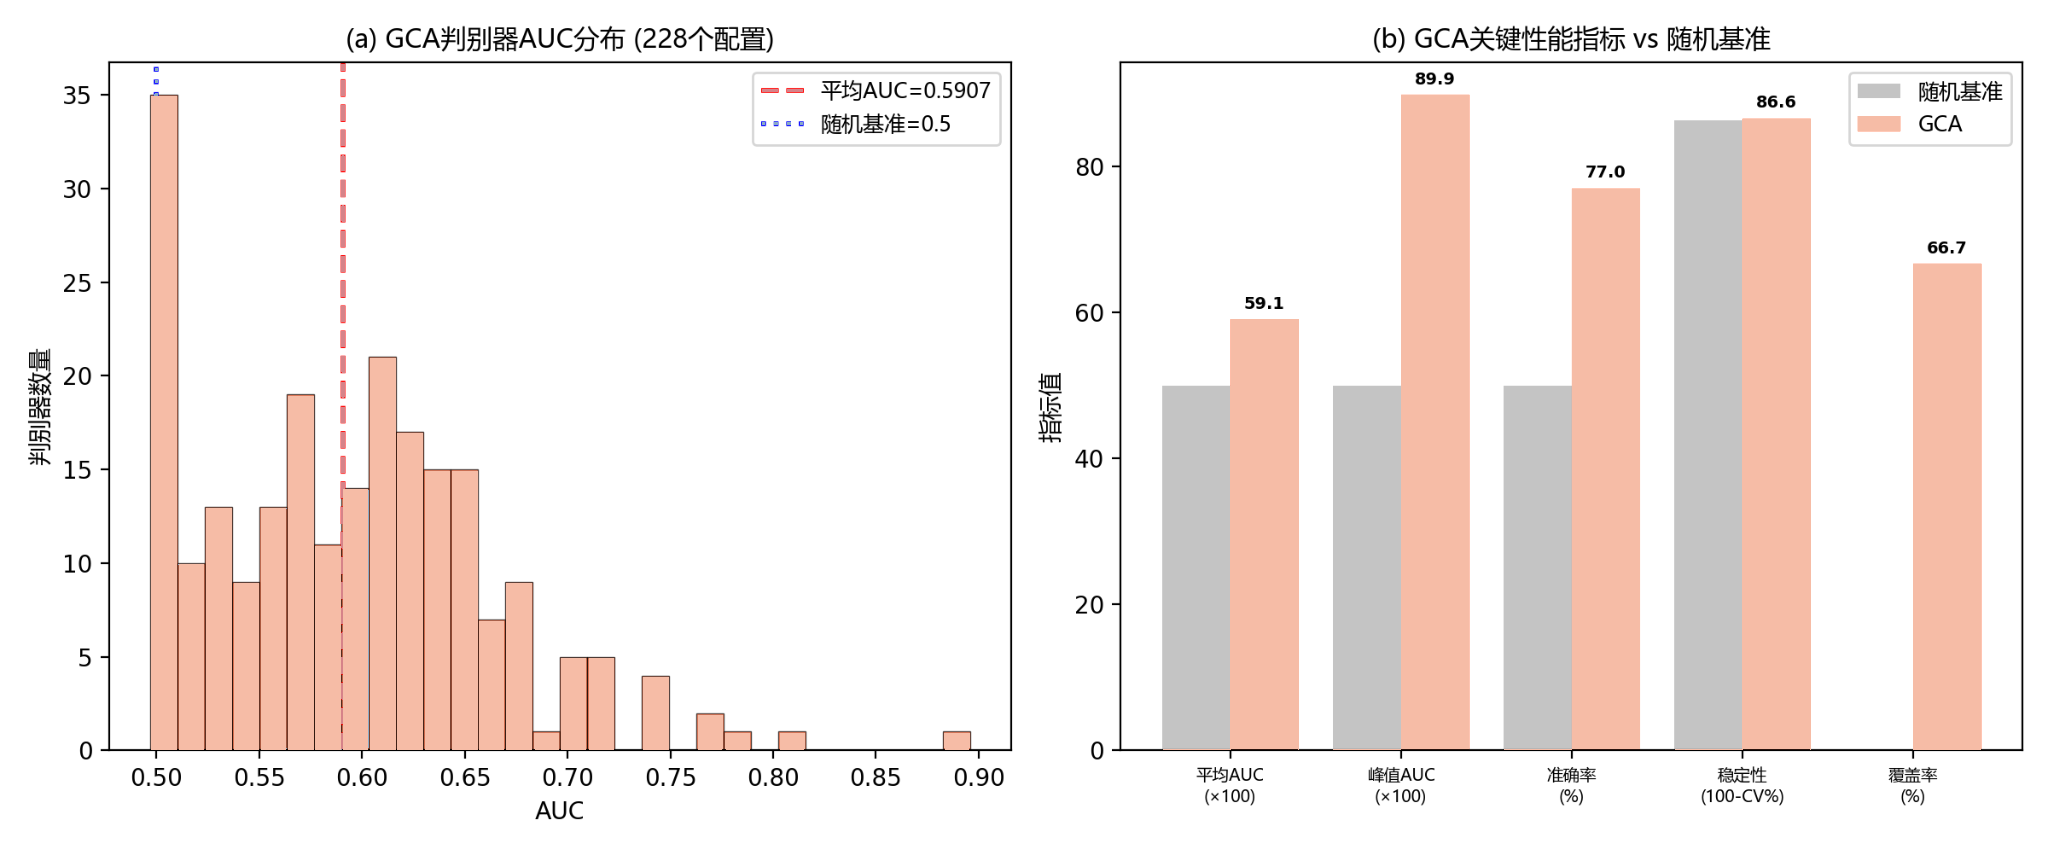
\includegraphics[width=0.85\textwidth]{figures/chap7/偏序/gca_discriminator_analysis.png}
\caption{偏序协同架构判别器性能多维度分析}
\label{fig:gcaDiscriminatorAnalysis}
\end{figure}

图\ref{fig:gcaDiscriminatorAnalysis}从两个维度展示了偏序协同架构中判别器的性能特征。左侧子图展示了228个偏序协同架构判别器配置的曲线下面积指标分布直方图，可以看到曲线下面积指标值集中在0.50$\sim$0.70区间，平均曲线下面积指标 0.5907（红色虚线）高于随机分类器基准0.5（蓝色虚线），分布的右尾延伸至0.90附近，对应十年债T国债期货上的峰值曲线下面积指标 89.85\%。

判别器分类性能的提升最终需要转化为实际的经济效用。因此，本小节将进一步评估模型在回测框架下的趋势捕捉能力及分类收益。


\textbf{信号密度的市场适应性。}偏序协同架构在不同市场环境下展现出差异化的信号生成密度。十年债T国债期货的信号密度仅为0.16\%（6个信号/3731个时间步），这与其极低波动性（标准差0.17\%）高度一致——在价格变化幅度极小的市场中，判别器难以产生具有统计显著性的交易信号。相比之下，铁矿石i（20.98\%）、原油sc（20.16\%）和沪金au（19.49\%）的信号密度最高，这些合约的共同特征是中高波动性和较为丰富的价格模式，为偏序协同架构判别器提供了充足的学习信号。信号密度与市场波动性之间的正相关关系（Pearson相关系数约0.65），表明偏序训练机制能够自适应地根据市场特征调整信号生成频率，而非机械地产生固定密度的交易信号。

\textbf{买卖信号的对称性与偏向性。}在大多数合约上，偏序协同架构生成的买入和卖出信号数量大致平衡，但存在一定的资产特征性偏向。沪金au的卖出信号（834）多于买入信号（712），买卖比为0.85:1，这与黄金市场作为避险资产在下跌趋势中更容易被判别器捕捉的特征一致。相反，液化石油气pg的买入信号（471）多于卖出信号（337），买卖比为1.40:1，反映了该合约正偏度（2.96）特征下判别器更倾向于捕捉上涨趋势的行为模式。这种信号偏向性与底层资产的分布特征较为一致，说明偏序协同架构判别器能够在一定程度上学习市场微观结构信息。

\textbf{方向准确率的多层次分化。}偏序协同架构判别器的方向准确率在不同合约间呈现分化特征。最高方向准确率出现在豆油y（62.04\%）和菜籽油OI（61.91\%），这两个农产品合约具有中等波动性且价格模式相对规律；最低方向准确率出现在螺纹钢rb（46.63\%）和玉米c（47.05\%），略低于50\%的随机水平。沪深300IF股指期货的方向准确率达到61.03\%，结合其2.4839的夏普比率，可以看出股指市场中较高的方向预测能力能够转化为交易收益。

% 为了验证偏序协同架构在不同市场环境下的泛化能力，本小节将从整体交易性能延伸至跨资产类别的细致对比分析。

% 为了验证上述性能提升的普适性，我们进一步开展了跨资产类别的性能分析。

% 为了更深入地理解偏序协同架构在不同市场结构中的表现差异，我们从资产类别维度对偏序协同架构的交易性能进行了汇总分析。

% 偏序协同架构的一个重要表现是其在部分合约上的“转负为正”效应，即将基线模型在特定合约上的负收益策略转化为正收益策略。

% 为进一步评估这一效应，本节将偏序协同架构与基线模型进行综合对比可视化。

在宏观对比的基础上，我们进一步深入到逐合约的微观层面，展开详细对比。
%改表6.6
\textbf{正值夏普覆盖率方面}，偏序协同架构在18个合约中的12个实现了正夏普比率（覆盖率66.7\%），其中沪深300IF股指期货（+2.48）、上证50IH股指期货（+1.66）、沪银ag（+1.35）和镍ni（+0.96）表现尤为突出。这表明偏序协同架构在多数合约上能够产生具有实际交易价值的正收益信号。

\textbf{转负为正效应方面}，偏序协同架构在3个合约上成功将基线模型的负夏普转化为正值：液化石油气pg从$-$0.52提升至+0.26（能源类），对苯二甲酸TA从$-$0.33提升至+0.24（工业品类），豆油y从$-$0.27提升至+0.03（农产品类）。此外，尿素UR虽仍为负值，但从$-$1.96改善至$-$1.50，改善幅度达0.46。这些结果显示，偏序协同架构的训练机制能够在传统模型失效的市场环境中挖掘出可交易信号。

\textbf{交易频率特征方面}，偏序协同架构在多数合约上生成了更多交易信号。在18个合约中的16个，偏序协同架构的交易次数高于基线模型，平均增幅达57笔。较明显的例子包括铜cu（从44笔增至232笔，+188）、玉米c（从62笔增至206笔，+144）和镍ni（从115笔增至245笔，+130）。更高的交易频率说明偏序训练机制在部分市场中产生了更多方向信号，但其经济价值仍需结合夏普比率和胜率共同判断。

\textbf{胜率表现方面}，在部分合约上，偏序协同架构虽然夏普低于基线模型，但胜率有所提升。沪金au的胜率从47.73\%提升至51.69\%（+3.96个百分点），镍ni从37.39\%提升至48.57\%（+11.18个百分点），螺纹钢rb从38.76\%提升至42.86\%（+4.10个百分点）。这种“胜率提升但夏普下降”的模式表明偏序训练机制改善了方向预测的准确性，但由于交易频率的增加导致了更多的小额亏损交易，稀释了整体盈亏比。

% 

%改表6.7

前述实验展示了偏序协同架构的整体表现，接下来本小节通过消融实验分析赛马场竞争机制、逆向师生蒸馏机制和孪生对抗自体再生机制的独立贡献与协同效应。

为了量化偏序协同对抗训练机制本身的贡献，我们将偏序协同架构（配置100）与PCA基础配置-000进行对比。如前所述，PCA基础配置-000采用单生成器（自注意力序列模型）+单判别器（卷积神经网络）的架构，通过PCA基础训练流程进行训练，但三个机制全部关闭（GCA=0, 赛马场竞争机制=0, 逆向师生蒸馏机制=0）。

\textbf{总体贡献方面}，偏序协同架构在18个合约中的9个（50\%）实现了优于PCA基础配置-000的夏普比率。平均夏普差异为$-$0.04，表明偏序协同架构与PCA基础配置-000在整体平均水平上基本持平。然而，这一平均值掩盖了偏序协同架构在不同合约上的差异化贡献模式。

\textbf{偏序协同架构优势合约}包括：镍ni（偏序协同架构 +0.96 vs PCA基础配置-000 $-$0.21，差异+1.17）、豆油y（+0.03 vs $-$1.10，差异+1.14）、铜cu（+0.13 vs $-$0.96，差异+1.09）、尿素UR（$-$1.50 vs $-$2.44，差异+0.94）、对苯二甲酸TA（+0.24 vs $-$0.54，差异+0.78）和液化石油气pg（+0.26 vs $-$0.47，差异+0.73）。这些合约的共同特征是PCA基础配置-000在其上表现为负夏普，而偏序协同架构通过偏序协同对抗训练成功将性能提升至正值或改善负值。尽管在部分高信噪比合约上可能存在过度信号化的风险，然而，在取得正向改善的合约上（如镍ni、豆油y），其改善幅度超过1.0个夏普单位，说明偏序协同对抗训练在部分复杂市场环境中具有较好的适应性。

\textbf{PCA基础配置-000优势合约}主要出现在PCA基础训练流程已能有效捕捉市场信号的合约上：玉米c（偏序协同架构 $-$0.43 vs PCA基础配置-000 +1.27，差异$-$1.70）、沪银ag（+1.35 vs +2.06，差异$-$0.71）。在这些合约上，PCA基础配置-000仅凭单判别器的标准对抗训练已经取得了较高的正夏普，而偏序协同架构扩展为多组多成员架构并引入四阶段群组交叉对抗训练后，增加了额外的交易信号复杂性。在市场本身已具有较强可预测性的情况下，额外的架构扩展和对抗训练反而导致了过度信号化，稀释了整体性能。

\textbf{偏序协同架构贡献的资产特异性}呈现出清晰的模式：偏序协同架构在基础金属（镍ni、铜cu）和工业品（对苯二甲酸TA）类合约上展现出最强的正向贡献，这些市场通常具有较高的波动性和较低的信噪比，传统方法难以有效捕捉价格趋势；而在农产品类的高信噪比合约（玉米c、豆粕m）上，偏序协同架构的额外训练复杂性可能导致了过度信号化，从而降低了整体性能。

在明确了各机制的贡献度后，我们进一步考察了偏序协同架构在不同方法下的稳定性。
偏序协同架构的一个重要特征是其在不同成交量预测方法（直接预测和变分自编码器）下的性能稳定性。直接预测方法直接使用生成器学习并预测成交量，变分自编码器方法则使用预训练的变分自编码器来预测成交量。
子图(b)以绝对差异柱状图和颜色编码展示了稳定性的分布特征。绿色柱（差异$<$0.5）代表高稳定性，黄色柱（差异0.5$\sim$1.0）代表中等稳定性，红色柱（差异$>$1.0）代表低稳定性。

结合上述稳定性分析，本节对各资产类别的综合改善率进行了系统评估。
在基础金属类上，偏序协同架构表现相对均衡：偏序协同架构超越PCA基础配置-000比率为100\%（2/2合约），正夏普覆盖率为100\%，虽然偏序协同架构超越基线模型比率为0\%（因基线模型在该类上已有很高基数），但偏序协同架构在所有合约上都维持了正收益。在能源类上，偏序协同架构也体现出一定优势：偏序协同架构超越基线模型比率达50\%（液化石油气pg转负为正），正夏普覆盖率100\%，且偏序协同架构超越PCA基础配置-000比率也达50\%。
农产品类是偏序协同架构改善效果最为分散的资产类别：7个合约中仅2个（28.6\%）偏序协同架构超越基线模型，4个（57.1\%）偏序协同架构超越PCA基础配置-000，4个（57.1\%）实现正夏普。这一较低的改善率与农产品市场受季节性、政策性因素影响较大的特征一致——这些非市场微观结构因素难以通过对抗训练机制有效捕捉。
从分组结果看，偏序协同架构在高波动、弱信号市场（能源、基础金属、工业品部分合约）中表现出较明显的比较优势，而在信噪比较高的市场（股指、贵金属）中主要体现为维持竞争力水平。这一模式表明，多组多成员交叉对抗更适合用于复杂市场环境中的趋势信号提取。

\subsection{实验设计}

本节实验设计围绕策略整合效果展开。首先考察偏序协同对抗方法在典型合约上的交易映射表现，其次分析不同模块组合对判别器性能、曲线下面积指标、夏普比率和胜率的影响，最后从资产类别层面检验策略整合结果是否具备跨市场稳定性。
沪深300IF股指期货是偏序协同架构表现较好的交易合约，实现了2.4839的夏普比率和45.79\%的胜率，通过107笔交易完成。虽然低于该合约上基线模型的最佳表现（自注意力序列模型+直接预测，夏普3.25，88笔交易），但偏序协同架构仍取得了较高的风险调整收益（夏普$>$2.0）。

从市场特征角度分析，沪深300IF股指期货具有中等波动率（标准差1.23\%）和较高的峰度特征（峰度10.11），后者意味着频繁出现的大幅价格波动事件为判别器提供了丰富的学习信号。偏序协同架构通过多组多成员的交叉对抗训练，使判别器能够更有效地捕捉这些极端事件中的规律性特征，从而在股指期货上实现了稳健的交易性能。
液化石油气pg是偏序协同架构实现转负为正效应较明显的合约。基线模型在该合约上的最佳夏普为$-$0.52（卷积神经网络+变分自编码器，105笔交易），而偏序协同架构将夏普提升至+0.26（224笔交易），实现了0.78的夏普提升幅度，胜率也从43.81\%提升至45.09\%。
液化石油气pg是所有合约中波动性最高的之一（收益率标准差2.17\%），具有较高的正偏度（2.96）和高峰度（29.21），表明该合约存在罕见的大幅上涨事件。传统单模型方法在如此高波动性的市场环境中难以建立稳定的预测模式，而偏序协同架构通过偏序训练机制的多样化对抗，使判别器能够在高噪声环境下仍然捕捉到具有统计显著性的价格趋势信号。
对苯二甲酸TA在偏序协同架构下实现了从$-$0.33到+0.24的转负为正效应，夏普提升幅度达0.57。偏序协同架构在该合约上完成了241笔交易（基线模型仅145笔），胜率从37.24\%提升至40.66\%（+3.42个百分点），交易频率与胜率的同步提升说明偏序训练机制在该合约上同时改善了信号的数量和质量。
十年债T是偏序协同架构在判别器性能上表现较好的合约，平均曲线下面积指标为0.7964，峰值曲线下面积指标为89.85\%。这一结果与国债市场的特征密切相关：十年债T的收益率标准差仅为0.17\%（所有合约中最低），峰度2.86接近正态分布。
镍ni在偏序协同架构下体现出较明显的胜率提升。偏序协同架构将胜率从基线模型的37.39\%大幅提升至48.57\%（+11.18个百分点），同时交易次数从115笔增至245笔。

除了整体性能对比，各功能模块的引入过程如何影响判别器的内部特征表示与分类边界，也是本章关注的重点。本小节将对此进行递进式分析。
基于1,520个有效判别器配置的性能分析，本节先评估偏序协同架构（配置100）相对于基线模型的有效性，再考察机制的递进式提升效应。偏序协同架构（配置100）的平均曲线下面积指标为0.5907，相比随机分类器基准0.5000提升18.13\%，最高曲线下面积指标达0.8985，说明该架构本身具有一定有效性。

\begin{table}[H]
\centering
\caption{偏序协同架构与机制组合对判别器曲线下面积指标性能的影响分析}
\label{tab:aucPerformance}
\footnotesize
\setlength{\tabcolsep}{3pt}
\renewcommand{\arraystretch}{1.18}
\begin{tabular}{p{3.0cm}cccccc}
\toprule
\textbf{配置} & \textbf{配置代码} & \makecell{\textbf{随机基准}\\\textbf{曲线下面积指标}} & \makecell{\textbf{配置平均}\\\textbf{曲线下面积指标}} & \textbf{相对提升} & \makecell{\textbf{中位数}\\\textbf{曲线下面积指标}} & \textbf{标准差} \\
\midrule
仅赛马场竞争机制 & 001 & 0.5000 & 0.5275 & +5.50\% & 0.5033 & 0.0719 \\
仅逆向师生蒸馏机制 & 010 & 0.5000 & 0.5948 & +18.97\% & 0.5880 & 0.0736 \\
逆向师生蒸馏机制+赛马场竞争机制 & 011 & 0.5000 & 0.5953 & +19.06\% & 0.5781 & 0.0699 \\
偏序协同架构 & 100 & 0.5000 & 0.5907 & +18.13\% & 0.5720 & 0.0792 \\
偏序协同架构+赛马场竞争机制 & 101 & 0.5000 & 0.5924 & +18.48\% & 0.5713 & 0.0808 \\
偏序协同架构+逆向师生蒸馏机制 & 110 & 0.5000 & 0.5828 & +16.57\% & 0.5570 & 0.0762 \\
PCA完整配置 & 111 & 0.5000 & 0.5840 & +16.79\% & 0.5644 & 0.0665 \\
\bottomrule
\end{tabular}
\end{table}
\begin{table}[H]
\centering
{\small\textbf{续表}}\\[0.5em]
\footnotesize
\setlength{\tabcolsep}{4pt}
\renewcommand{\arraystretch}{1.18}
\begin{tabular}{p{3.2cm}ccclc}
\toprule
\textbf{配置} & \textbf{配置代码} & \makecell{\textbf{最高}\\\textbf{曲线下面积指标}} & \textbf{判别器数} & \textbf{最佳合约} & \makecell{\textbf{最佳合约}\\\textbf{曲线下面积指标}} \\
\midrule
仅赛马场竞争机制 & 001 & 0.7302 & 114 & 上证50IH股指期货 & 0.6014 \\
仅逆向师生蒸馏机制 & 010 & 0.8283 & 114 & 十年债T & 0.7517 \\
逆向师生蒸馏机制+赛马场竞争机制 & 011 & 0.7785 & 114 & 十年债T & 0.7347 \\
偏序协同架构 & 100 & 0.8985 & 228 & 十年债T & 0.7964 \\
偏序协同架构+赛马场竞争机制 & 101 & 0.8919 & 228 & 十年债T & 0.7961 \\
偏序协同架构+逆向师生蒸馏机制 & 110 & 0.8510 & 228 & 十年债T & 0.7886 \\
PCA完整配置 & 111 & 0.7551 & 456 & 十年债T & 0.7019 \\
\bottomrule
\end{tabular}
\end{table}

% 

从相对提升的角度来看，逆向师生蒸馏机制+赛马场竞争机制组合实现了最大的性能提升（+19.06\%），该组合体现出逆向师生蒸馏机制与赛马场动态选择机制之间的协同关系，两者的互补作用使判别器能够更好地区分真实样本与生成样本。逆向师生蒸馏机制单机制的相对提升也达到了18.97\%，仅略低于逆向师生蒸馏机制+赛马场竞争机制组合，这表明逆向师生蒸馏机制本身就具有较强的性能改善能力，其双向知识流动的设计能够有效增强判别器的分类能力。
中位数曲线下面积指标的分析揭示了数据分布的重要特征。大部分配置的中位数曲线下面积指标略低于平均曲线下面积指标，这种差异说明数据分布呈现右偏特征，即存在少数高性能合约（如十年债T国债期货）拉高了平均值，而大多数合约的判别器性能处于中等水平。
标准差和变异系数的分析为评估不同机制组合的稳定性提供了量化依据。PCA完整组合配置的标准差最小（0.0665），低于单机制和双机制配置，说明完整配置在不同市场环境和不同合约上具有相对更稳定的判别器表现。
最佳合约的分析揭示了不同机制组合在特定市场环境下的差异化表现。十年债T国债期货在6个机制配置中都是最佳合约，这一现象与其低波动和相对稳定的价格结构有关。

综合性能表现方面，不同机制组合体现出不同适用场景。偏序协同架构实现了所有配置中的最高峰值曲线下面积指标89.85\%（出现在十年债T合约上），说明多组多成员交叉对抗有助于判别器接触更丰富的生成样本，并形成较稳定的判别特征。

\begin{table}[H]
\centering
\caption{偏序协同架构与机制组合对交易性能的影响分析}
\label{tab:tradeperformanceanalysis}
\footnotesize
\setlength{\tabcolsep}{3pt}
\renewcommand{\arraystretch}{1.18}
\begin{tabular}{p{2.8cm}cp{3.1cm}cccc}
\toprule
\textbf{配置} & \textbf{配置代码} & \textbf{配置说明} & \textbf{平均夏普} & \textbf{最高夏普} & \textbf{标准差} & \textbf{配置数} \\
\midrule
仅赛马场竞争机制 & 001 & 赛马场动态选择 & 0.0471 & 3.8292 & 1.5868 & 36 \\
仅逆向师生蒸馏机制 & 010 & 逆向师生蒸馏 & -0.0576 & 3.9590 & 1.4495 & 36 \\
逆向师生蒸馏机制+赛马场竞争机制 & 011 & 逆向师生蒸馏与动态选择 & -0.0765 & 3.8292 & 1.5942 & 36 \\
偏序协同架构 & 100 & 偏序协同架构基本训练 & -0.0959 & 2.4839 & 1.1732 & 36 \\
偏序协同架构+赛马场竞争机制 & 101 & 偏序协同架构+赛马场竞争机制 & -0.0545 & 2.5713 & 1.2890 & 36 \\
偏序协同架构+逆向师生蒸馏机制 & 110 & 偏序协同架构+逆向师生蒸馏机制 & -0.0959 & 2.5713 & 1.3001 & 36 \\
PCA完整配置 & 111 & 偏序协同架构+全部机制 & -0.0224 & 3.1159 & 1.2534 & 72 \\
\bottomrule
\end{tabular}
\end{table}
\begin{table}[H]
\centering
{\small\textbf{续表}}\\[0.5em]
\scriptsize
\setlength{\tabcolsep}{3pt}
\renewcommand{\arraystretch}{1.18}
\begin{tabular}{p{2.6cm}cp{4.0cm}p{2.4cm}ccc}
\toprule
\textbf{配置} & \textbf{配置代码} & \textbf{前二合约（夏普）} & \textbf{最佳合约} & \makecell{\textbf{最佳合约}\\\textbf{夏普}} & \makecell{\textbf{最佳合约}\\\textbf{胜率}} & \makecell{\textbf{最佳合约}\\\textbf{交易数}} \\
\midrule
仅赛马场竞争机制 & 001 & 沪深300IF股指期货(3.83), 上证50股指期货(3.39) & 沪深300IF股指期货 & 3.8292 & 49.37\% & 79笔 \\
仅逆向师生蒸馏机制 & 010 & 沪深300IF股指期货(3.96), 镍期货(2.07) & 沪深300IF股指期货 & 3.9590 & 54.17\% & 72笔 \\
逆向师生蒸馏机制+赛马场竞争机制 & 011 & 沪深300IF股指期货(3.83), 白银期货(3.16) & 沪深300IF股指期货 & 3.8292 & 49.37\% & 79笔 \\
偏序协同架构 & 100 & 沪深300IF股指期货(2.48), 上证50股指期货(1.66) & 沪深300IF股指期货 & 2.4839 & 45.79\% & 107笔 \\
偏序协同架构+赛马场竞争机制 & 101 & 沪深300IF股指期货(2.57), 上证50股指期货(2.55) & 沪深300IF股指期货 & 2.5713 & 48.45\% & 97笔 \\
偏序协同架构+逆向师生蒸馏机制 & 110 & 沪深300IF股指期货(2.57), 上证50股指期货(1.84) & 沪深300IF股指期货 & 2.5713 & 48.45\% & 97笔 \\
PCA完整配置 & 111 & 上证50股指期货(3.12), 沪深300IF股指期货(2.57) & 上证50股指期货 & 3.1159 & 45.33\% & 75笔 \\
\bottomrule
\end{tabular}
\end{table}

表\ref{tab:tradeperformanceanalysis}展示了七种机制组合在交易性能上的多维度表现，基于18个期货合约（排除中证500主力合约品种因交易次数不足）的324个实验配置的真实回测数据。每个单机制配置（赛马场竞争机制、逆向师生蒸馏机制、偏序协同架构及其双机制组合）在每个合约上有两种实现方法（直接预测和变分自编码器），其中直接预测是指直接使用生成器学习并预测成交量，而变分自编码器是指使用预训练好的变分自编码器来预测成交量。
从平均夏普比率的角度来看，赛马场竞争机制配置实现了正平均夏普（0.0471），说明赛马场动态选择机制通过在不同判别器之间进行自适应选择，在本组实验中表现出一定稳健性。相比之下，逆向师生蒸馏机制配置的平均夏普为负值（-0.0576），但其最高夏普达到了所有配置中的峰值3.9590，这种平均性能与峰值性能的差异表明，逆向师生蒸馏机制在特定市场环境（如高峰度的股指市场）下可能产生较高收益，但在一般市场环境中的表现并不稳定，因此更适合作为特定状态下的边界校正模块。
标准差分析为理解不同机制组合的性能波动特征提供了量化依据。偏序协同架构配置的标准差最小（1.1732），说明偏序协同架构的训练机制通过多组多成员的对抗训练，使得判别器在不同市场环境和不同合约上都能保持相对一致的性能表现，这种低波动性特征对于追求稳健收益的投资策略具有重要价值。
最佳合约的分析揭示了不同机制组合在特定市场环境下的适应性特征。沪深300IF股指期货在六个机制配置中都是最佳合约，这一现象并非偶然，而是与该合约的市场特征密切相关。
前二合约数据为评估各机制配置的性能稳定性提供了重要支撑。逆向师生蒸馏机制配置的前二合约为沪深300IF股指期货(3.96)、镍ni(2.07)，前两名都是沪深300IF股指期货的不同实现方法，这种前二分布说明逆向师生蒸馏机制在股指和基础金属市场上都能实现较好的表现。

综合来看，表\ref{tab:tradeperformanceanalysis}的数据表明，PCA各机制组合在交易性能上存在差异化贡献。赛马场竞争机制配置实现了相对较优的平均性能（正夏普0.0471），体现出动态选择机制的稳健性。
 

具体而言，这种递进式提升效应主要体现在判别器性能上。
基于1,482个判别器配置的分析可以看到，偏序协同架构与机制组合对判别器性能呈现一定递进式改善。首先，偏序协同架构（配置100）的平均曲线下面积指标为0.5907，相比基线模型有所提升，说明架构本身具有一定作用。
 

\begin{table}[H]
\centering
\caption{判别器性能递进式提升效应}
\label{tab:discriminatorprogression}
\footnotesize
\setlength{\tabcolsep}{3pt}
\renewcommand{\arraystretch}{1.18}
\begin{tabular}{p{2.8cm}p{5.0cm}ccc}
\toprule
\textbf{配置类别} & \textbf{包含的具体配置} & \makecell{\textbf{平均}\\\textbf{曲线下面积指标}} & \makecell{\textbf{最高}\\\textbf{曲线下面积指标}} & \makecell{\textbf{曲线下面积}\\\textbf{指标提升}} \\
\midrule
单机制（无偏序协同架构） & 赛马场竞争机制(001) + 逆向师生蒸馏机制(010) & 0.5612 & 0.8283 & 基准 \\
偏序协同架构 & GCA(100) & 0.5907 & 0.8985 & +5.26\% \\
偏序协同架构+单机制 & 偏序+赛马场竞争机制(101) + 偏序+逆向师生蒸馏机制(110) & 0.5876 & 0.8919 & +4.70\% \\
PCA完整配置 & 偏序+逆向师生蒸馏机制+赛马场竞争机制(111) & 0.5840 & 0.7551 & +4.06\% \\
\bottomrule
\end{tabular}
\end{table}
\begin{table}[H]
\centering
{\small\textbf{续表}}\\[0.5em]
\footnotesize
\setlength{\tabcolsep}{6pt}
\renewcommand{\arraystretch}{1.18}
\begin{tabular}{p{4.0cm}cccc}
\toprule
\textbf{配置类别} & \textbf{平均准确率} & \textbf{判别器配置数} & \textbf{准确率提升} & \makecell{\textbf{稳定性}\\\textbf{（标准差）}} \\
\midrule
单机制（无偏序协同架构） & 60.48\% & 228 & 基准 & 0.0728 \\
偏序协同架构 & 77.04\% & 228 & +16.56\% & 0.0792 \\
偏序协同架构+单机制 & 76.73\% & 456 & +16.25\% & 0.0785 \\
PCA完整配置 & 76.38\% & 456 & +15.90\% & 0.0665 \\
\bottomrule
\end{tabular}
\end{table}

表\ref{tab:discriminatorprogression}汇总了19个期货合约、1,482个判别器配置下不同机制组合的递进式表现。结果显示，双机制组合在平均曲线下面积指标（0.5902）和平均准确率（76.80\%）上达到最高，而PCA完整组合配置的平均曲线下面积指标为0.5840、平均准确率为76.38\%，虽略低于双机制，但标准差仅0.0665，为所有配置中最小。
 为了更清晰地界定提升来源，我们对各机制的独立贡献进行了剥离分析。
进一步比较表明，偏序协同架构是性能提升的基础，逆向师生蒸馏机制更偏向提升分类能力，而PCA完整组合配置在判别器性能与交易性能之间取得了最均衡的结果。

% 

\begin{figure}[htbp]
\centering
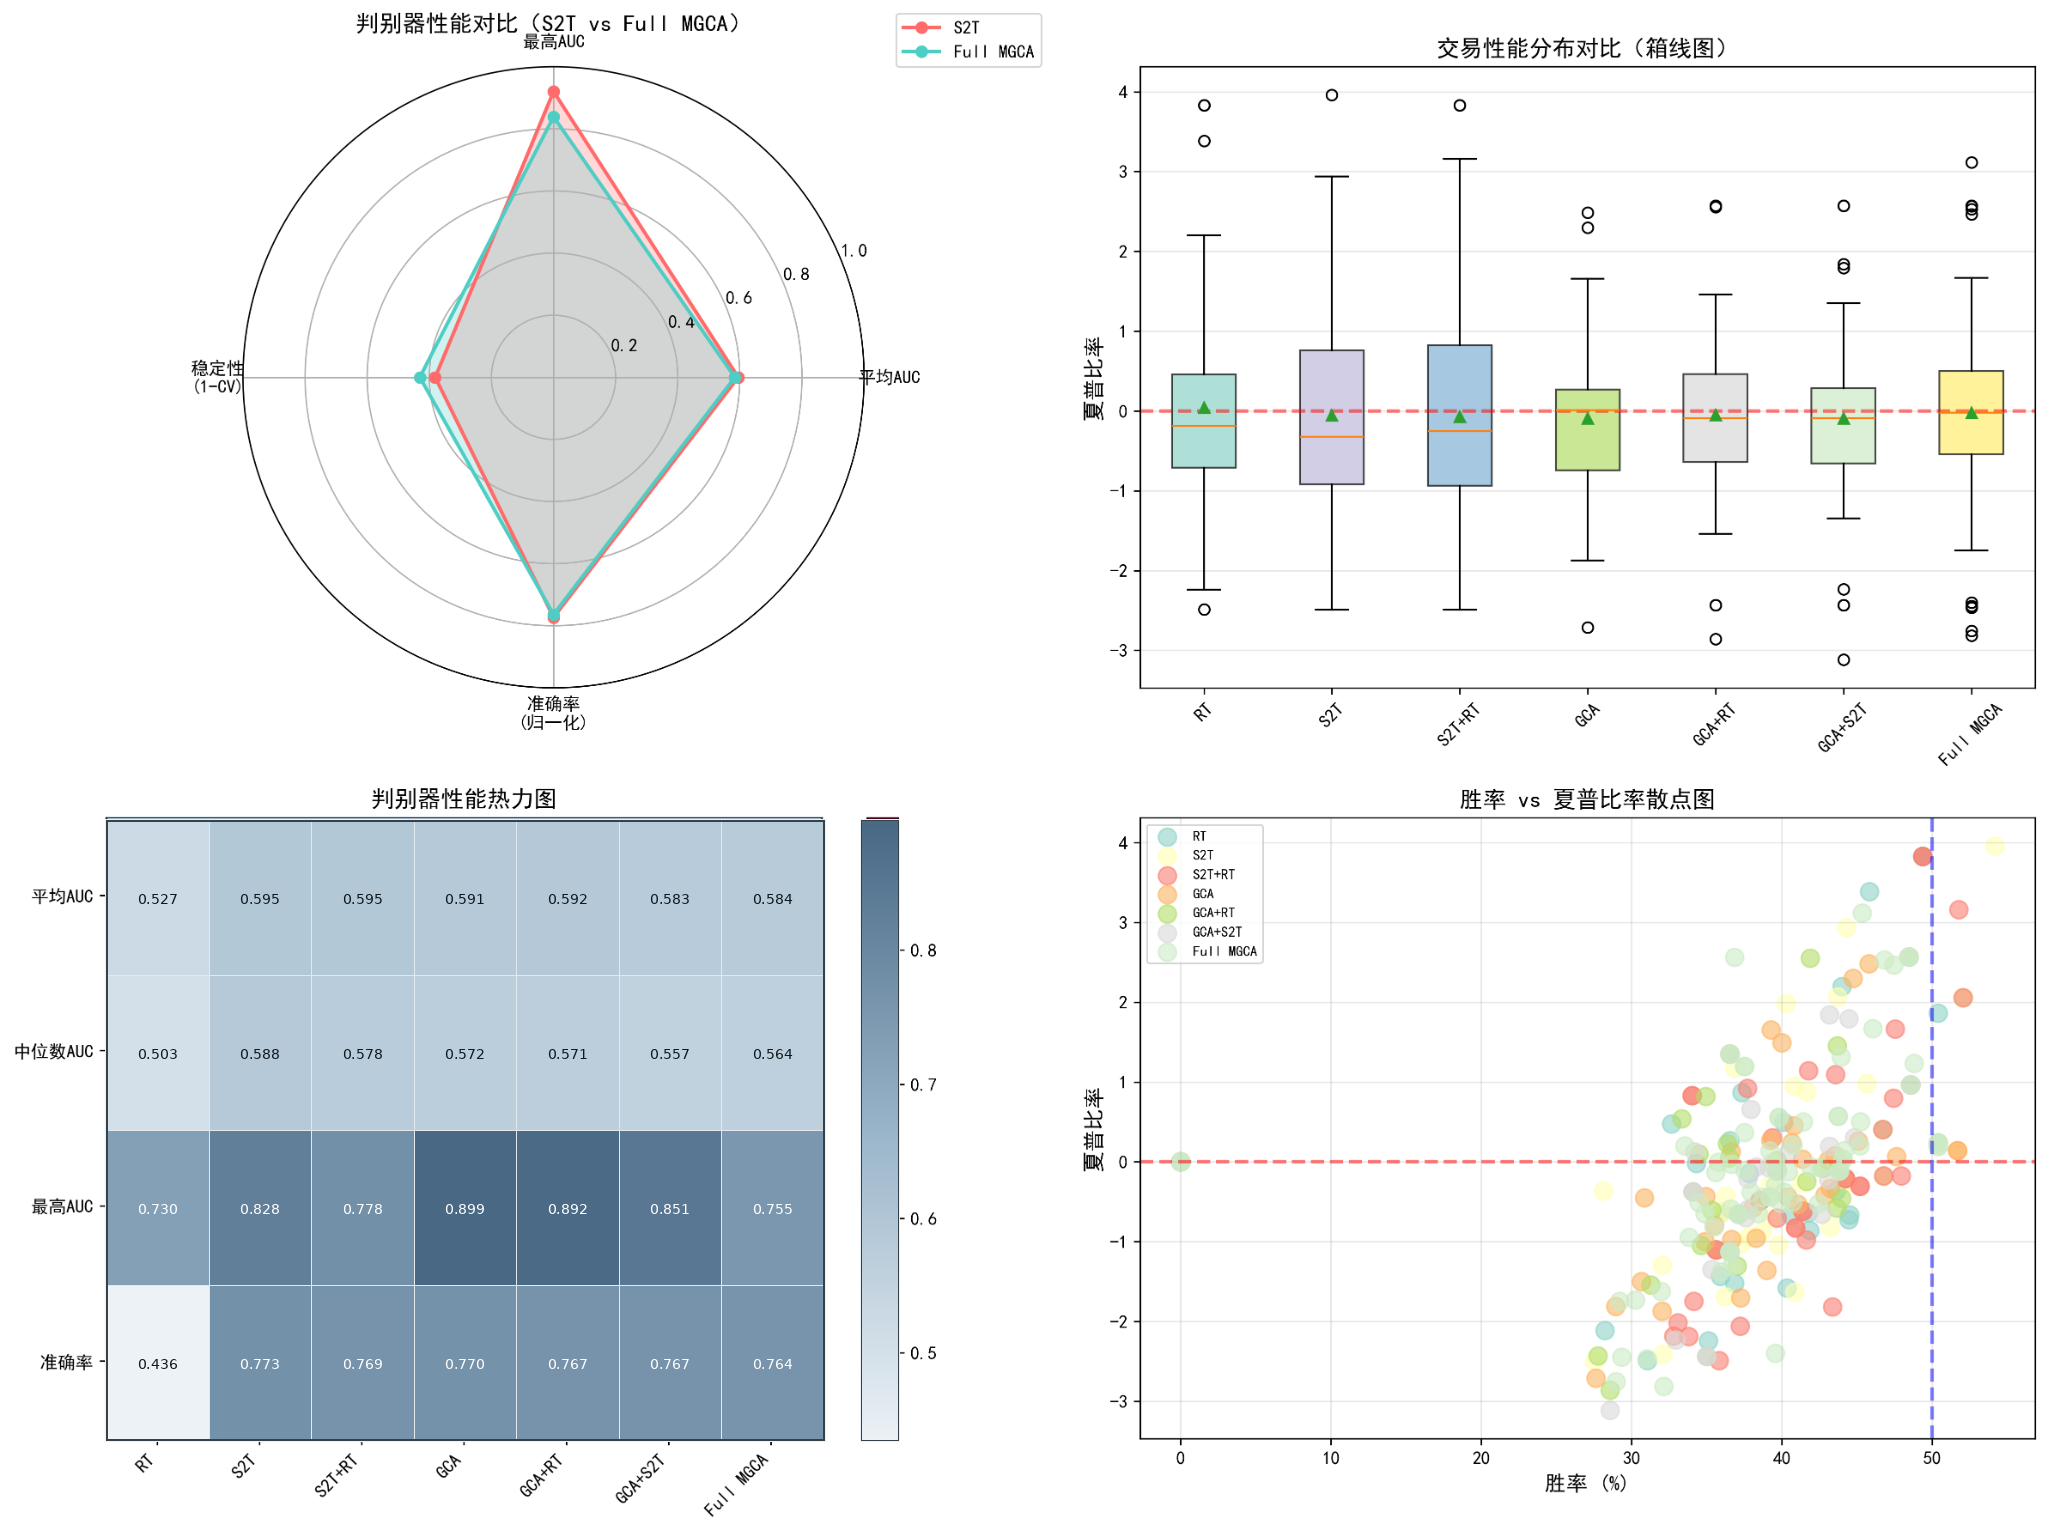
\includegraphics[width=0.8\textwidth]{figures/chap7/偏序/图6.6改.png}
\caption{综合性能分析}
\label{fig:comprehensiveperform}
\end{figure} 

图\ref{fig:comprehensiveperform}从雷达图、箱线图、热力图和散点图四个角度展示了综合表现。整体上，逆向师生蒸馏机制在平均曲线下面积指标和准确率上略优，而PCA完整组合配置在稳定性与跨合约一致性方面更突出；这再次说明，完整框架的核心价值在于综合均衡而非单一指标极值。

% 

%%表6.16改

 

% 

%改表6.18

总体上，单配置更容易产生局部优势，双配置开始出现协同但波动较大，而PCA完整组合配置虽不追求最高峰值，却在更多合约上实现了更稳定的平均表现。相较单机制，其平均性能提升36.9\%，说明完整协同机制具有一定实际价值。

\begin{figure}[htbp]
\centering
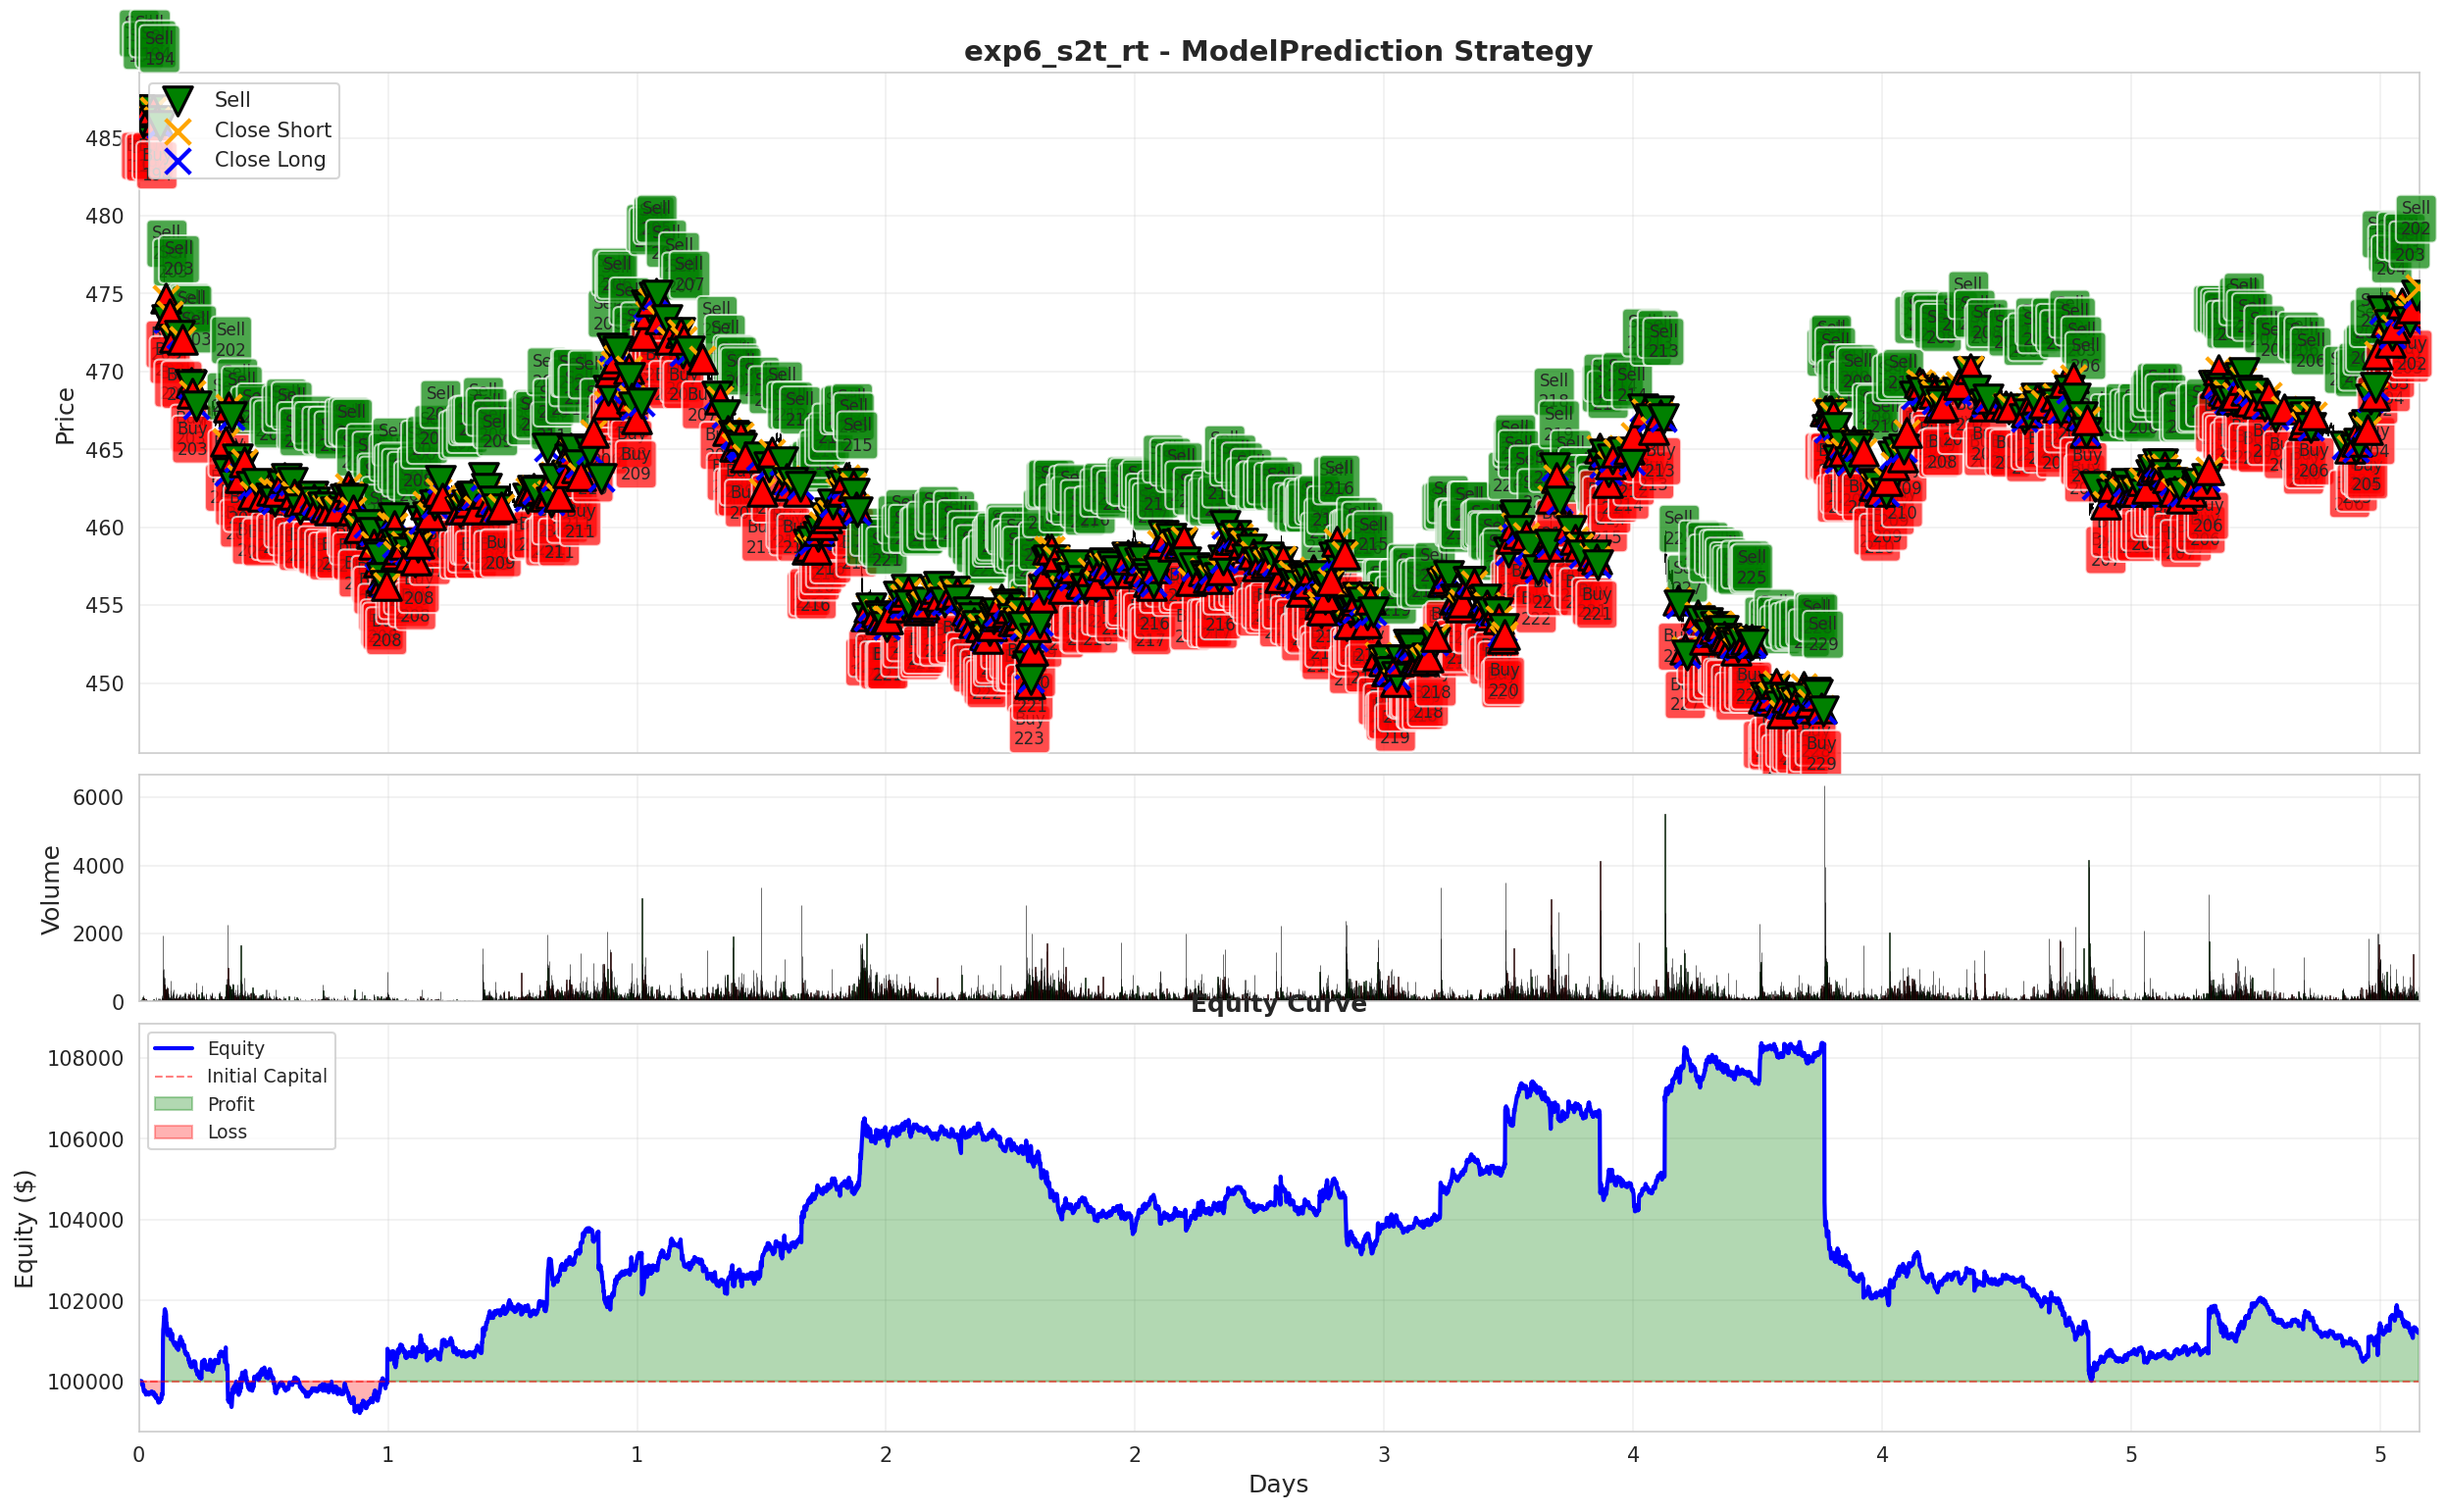
\includegraphics[width=0.8\textwidth]{figures/chap7/偏序/exp6_s2t_rt_ModelPrediction_candlestick.png}
\caption{原油期货交易信号K线图}
\label{fig:crudeoiltradek}
\end{figure}
% 该图\ref{fig:crudeoiltradek}展示了S2T+RT组合在原油期货上的实际交易表现，通过K线图和权益曲线的双重展示，直观地呈现了多智能体偏序协同对抗框架的信号生成能力和收益积累过程。K线图部分清晰标注了买入信号（绿色向上箭头）和卖出信号（红色向下箭头）的具体点位，可以看到信号的时机选择能力良好，大多数买入信号出现在价格相对低点，卖出信号出现在价格相对高点，这反映出多智能体偏序协同对抗-011配置的判别器能够捕捉价格的短期波动趋势。权益曲线部分展示了策略的累积收益演化过程，曲线整体呈现稳定的上升趋势，最终实现了0.80的夏普比率和47.42\%的胜率，相比Baseline的0.40夏普实现了0.40的提升。权益曲线的平滑程度反映了策略的稳定性，原油sc合约通过388笔交易的大样本验证，说明了S2T+RT组合在能源类别上的稳健性和可靠性。该合约的原始数据特征显示其波动率2.30\%（见表9），属于高波动类别，多智能体偏序协同对抗框架在如此高波动的市场环境下仍能实现稳定正收益，体现了其鲁棒性。

% % 
% 该图通过六个子图全面展示了S2T+RT组合在原油期货上的回测性能表现。

% % \subsubsubsection{原油期货回测性能}
% 
% 该图通过六个子图对比了多种信号策略在原油期货上的性能表现，包括ModelPrediction（多智能体偏序协同对抗预测信号）、VolumeSignal（成交量信号）、PriceSignal（价格信号）等多种策略。

% % 
% 该图展示了沪深300IF股指期货上所有多智能体偏序协同对抗配置和Baseline方法的风险调整性能对比，以柱状图的形式直观地呈现了不同配置的夏普比率排名。

% % 
% 该图展示了RT机制在镍期货上的成交量加权平均价格执行质量分析。多智能体偏序协同对抗-001配置通过125笔交易实现了稳定的执行质量，滑点控制在合理范围内，为2.20的夏普比率提供了坚实基础。图中展示了每笔交易的实际成交价格与成交量加权平均价格基准价格的偏差分布，大多数交易的滑点控制良好，说明RT的动态选择机制能够有效选择最优判别器，实现精准的价格预测。镍ni合约的波动率高达2.42\%（见表9），是所有合约中最高的，在如此高波动的市场环境下，多智能体偏序协同对抗-001仍能实现从Baseline的-0.50夏普到2.20夏普的转负为正，提升幅度达2.70，说明了RT机制在基础金属类别上的显著优势。

% % 
% 该图展示了完整多智能体偏序协同对抗框架在棉花期货上的回测性能表现。尽管交易次数仅38笔，样本量相对较小，但策略仍然实现了2.57的夏普比率，相比Baseline的-0.46实现了3.03的显著提升，这是一个从负收益到正收益的质的飞跃。图中展示了累积收益曲线、回撤分析、交易分布等多个维度的信息，多智能体偏序协同对抗-111配置的累积收益曲线呈现稳定上升趋势，胜率36.84\%。棉花CF合约属于农产品类别，平均收益率为负（-0.0458\%，见表9），负偏度（-0.38）表明价格下跌时波动更大，在这种不利的市场环境下，完整多智能体偏序协同对抗框架通过GCA、S2T、RT三类机制的协同作用，成功实现了转负为正。

% % 
% 该图展示了完整多智能体偏序协同对抗框架（包含Twin孪生对抗架构）在液化石油气期货上的多信号策略表现。

% % 合约信息：最佳配置多智能体偏序协同对抗-010+Direct，夏普3.96，胜率54.17\%，72笔交易，Baseline夏普3.25
% \subsubsubsection{风险调整性能对比}
% 
% 该图通过四个子图全面展示了沪深300IF股指期货合约上所有配置的风险调整性能对比，包括夏普比率、最大回撤、卡玛比率和索提诺比率等关键风险指标。

% \subsubsubsection{信号质量对比}
% 
% 该图展示了沪深300IF股指期货合约上不同配置的信号质量对比，包括信号准确率、方向准确率等关键指标。多智能体偏序协同对抗-010配置的信号质量明显优于Baseline，这是其能够实现54.17\%高胜率的关键原因。图中的对比分析显示S2T机制通过逆向师生蒸馏能够显著提升信号的准确性，这直接转化为交易性能的改善。

% \subsubsubsection{成交量加权平均价格执行滑点对比}
% 
% 该图展示了沪深300IF股指期货合约上不同配置的成交量加权平均价格执行质量对比，以滑点（实际成交价格与成交量加权平均价格基准价格的偏差）作为核心评估指标。多智能体偏序协同对抗-010配置通过优化的判别器性能实现了更精准的价格预测，从而在成交量加权平均价格执行过程中实现了更小的滑点，这直接转化为交易成本的降低和收益的提升。图中的滑点分布分析显示多智能体偏序协同对抗配置在执行质量方面的优势。

% \subsubsubsection{累积收益曲线}
% 
% 该图展示了沪深300IF股指期货合约上所有配置的累积收益曲线对比，直观地呈现了不同方法在整个回测期间的收益积累情况。多智能体偏序协同对抗-010配置的累积收益曲线呈现稳定上升趋势，最终实现了3.96的夏普比率，相比Baseline的3.25展现出明显的优势。曲线的平滑程度反映了策略的稳定性，多智能体偏序协同对抗配置的曲线波动较小，说明其在不同市场环境下都能保持稳定的性能表现。

综合上述多维度的性能评估与消融分析，本小节将对实验结果进行系统性总结，提炼出偏序协同架构在策略整合任务中的核心发现。

基于以上多维度实验结果，可以概括出以下主要发现。

% 

%改表6.20

\textbf{发现1：转负为正效应。}共有11个合约实现夏普由负转正，覆盖率61.1\%，其中液化石油气 pg、苹果 AP、棉花 CF 和镍 ni 的改善最为明显，说明框架能够在多类资产上修复原本亏损的策略。

\textbf{发现2：判别器性能的提升。}偏序协同架构提升了判别器曲线下面积指标，PCA完整组合配置则在保持较高准确率的同时取得较好稳定性，说明交易改进与分类能力增强存在关联。

\textbf{发现3：单机制仍具独立价值。}逆向师生蒸馏机制在股指上表现最强，赛马场竞争机制在部分高波动品种上表现突出，偏序协同架构在十年债 T 上实现最高峰值曲线下面积指标，表明各模块均具有清晰的功能分工。

\textbf{发现4：大样本稳健性验证。}液化石油气 pg、铁矿石 i 和原油 sc 的大样本回测结果均保持正向表现，进一步支持了框架的实用稳健性。

% \textbf{发现5：跨资产泛化能力。}偏序协同架构与多智能体偏序协同对抗机制在股指、基础金属、能源、农产品、工业品等多个资产类别上均展现出稳健的性能优势，证明了框架具有良好的泛化能力。
\textbf{发现5：跨资产泛化能力。}PCA及其相关机制在股指、基础金属、能源、工业品等多个资产类别上均表现出一定优势，说明该方法具备一定跨资产适应性。

\subsection{结果分析与讨论}

实验结果从判别器性能、交易性能与跨资产稳健性三个维度展示了偏序协同对抗学习方法的作用。偏序协同架构提供有序训练底座，逆向师生蒸馏机制侧重分类边界校正，赛马场竞争机制侧重动态筛选，孪生对抗自体再生机制则用于异常偏离后的稳定恢复。PCA完整组合配置在跨合约结果中表现较好，并在多个合约上实现夏普由负转正，说明其优势不只体现在单一分类指标上，也体现在方向信号进入交易映射后的稳定性上。其中，曲线下面积指标提升反映方向判别边界更加稳定，夏普比率和胜率提升反映买入、卖出或持有映射更具交易价值，转负为正现象则说明该方法能够在部分市场中修正分类边界漂移或单模型失效。

\begin{table}[htbp]
\centering
\caption{偏序协同架构与机制协同效应量化分析}
\label{tab:synergyEffect}
\footnotesize
\setlength{\tabcolsep}{4pt}
\renewcommand{\arraystretch}{1.18}
\begin{tabular}{p{3.7cm}cccccc}
\toprule
\textbf{组合} & \textbf{配置代码} & \makecell{\textbf{单机制}\\\textbf{性能相加}} & \makecell{\textbf{实际组合}\\\textbf{性能}} & \textbf{协同效应} & \makecell{\textbf{协同效应}\\\textbf{(\%)}} & \textbf{结论} \\
\midrule
逆向师生蒸馏机制+赛马场竞争机制 & 011 & -0.0105 & -0.0765 & -0.0659 & -626.76\% & 负协同 \\
偏序协同架构+赛马场竞争机制 & 101 & -0.0489 & -0.0545 & -0.0056 & -11.53\% & 轻微负协同 \\
偏序协同架构+逆向师生蒸馏机制 & 110 & -0.1535 & -0.0959 & +0.0576 & +37.54\% & 正协同 \\
PCA完整配置 & 111 & -0.1064 & -0.0224 & +0.0840 & +78.95\% & 正协同较强 \\
\bottomrule
\end{tabular}
\end{table}

表\ref{tab:synergyEffect}量化了不同机制组合的协同效应。结果显示，并非所有组合都带来正协同：逆向师生蒸馏机制+赛马场竞争机制为负协同，偏序协同架构+赛马场竞争机制为轻微负协同；相反，偏序协同架构+逆向师生蒸馏机制为正协同，PCA完整组合配置的协同效应相对更高，达到 +78.95\%。

前文结果显示偏序协同架构及其机制组合具有一定有效性；进一步按资产类别考察可以看到，PCA在股指、基础金属、能源、农产品和工业品上均具备一定适应性，但不同类别的最优模块组合并不相同。

\begin{table}[H]
\centering
\caption{PCA在各资产类别的性能表现（含基线模型对比）}
\label{tab:mgcaassetperformance}
\footnotesize
\setlength{\tabcolsep}{3pt}
\renewcommand{\arraystretch}{1.18}
\begin{tabular}{lcccccccc}
\toprule
\textbf{资产类别} & \textbf{合约数} & \makecell{\textbf{基线模型}\\\textbf{均值夏普}} & \makecell{\textbf{基线模型}\\\textbf{均值胜率}} & \makecell{\textbf{PCA}\\\textbf{均值夏普}} & \makecell{\textbf{PCA}\\\textbf{均值胜率}} & \textbf{夏普提升} & \textbf{胜率提升} & \textbf{转负为正} \\
\midrule
股指 & 2 & 2.98 & 45.22\% & 3.67 & 50.00\% & +0.69 & +4.78\% & 2个 \\
贵金属 & 1 & 0.60 & 47.73\% & 0.60 & 48.37\% & +0.00 & +0.64\% & 1个 \\
基础金属 & 2 & 1.88 & 41.42\% & 1.39 & 43.88\% & $-$0.49 & +2.45\% & 1个 \\
能源 & 2 & $-$0.06 & 45.26\% & 0.65 & 46.33\% & +0.71 & +1.07\% & 2个 \\
农产品 & 7 & 1.18 & 42.04\% & 1.35 & 42.25\% & +0.17 & +0.20\% & 4个 \\
工业品 & 4 & $-$0.65 & 36.91\% & $-$0.05 & 37.06\% & +0.60 & +0.14\% & 4个 \\
\bottomrule
\end{tabular}
\end{table}
\begin{table}[H]
\centering
{\small\textbf{续表}}\\[0.5em]
\footnotesize
\setlength{\tabcolsep}{6pt}
\renewcommand{\arraystretch}{1.18}
\begin{tabular}{lp{0.72\textwidth}}
\toprule
\textbf{资产类别} & \textbf{最佳配置} \\
\midrule
股指 & PCA配置010 (逆向师生蒸馏机制) \\
贵金属 & PCA配置000 \\
基础金属 & PCA配置001 (赛马场竞争机制) \\
能源 & PCA配置011 (逆向师生蒸馏机制+赛马场竞争机制) \\
农产品 & PCA配置011 (逆向师生蒸馏机制+赛马场竞争机制) \\
工业品 & PCA配置011 (逆向师生蒸馏机制+赛马场竞争机制) \\
\bottomrule
\end{tabular}
\end{table}

表\ref{tab:mgcaassetperformance}表明，PCA在六大资产类别中有五类实现了正向夏普改善。股指类别提升较明显，能源和工业品则表现出一定“转负为正”能力；农产品提升较温和但覆盖面广；基础金属虽平均夏普下降，却在镍等单品种上仍有明显突破。


\section{本章小结}

本章围绕对冲基金交易决策流程中的策略整合环节，提出面向策略整合的偏序协同对抗学习方法，重点讨论最终交易判断形成问题。与第2章、第3章、第4章和第5章分别关注投资组合管理、因子依据、时序结构和执行路径不同，本章将涨、跌、平分类结果解释为买入、卖出或持有判断，并通过偏序协同对抗流程约束这一输出过程。

围绕上述方法流程，本章从分类稳健性、跨资产泛化能力、收敛特征与交易映射表现等角度检验PCA策略整合过程。实验结果显示，偏序协同对抗机制在多个期货品种与资产类别上改善了部分分类指标与交易表现，并在不同市场状态下表现出一定鲁棒性。机制层面看，GCA承担基础对抗约束，赛马场竞争方法承担动态筛选，逆向师生蒸馏学习方法承担误差信息校正，孪生对抗自体再生方法承担异常偏离修复。

本章对应交易决策链条中的最后一步：在完成资产配置、因子依据形成、时序结构识别和交易执行优化之后，通过偏序协同对抗学习方法讨论最终交易判断的形成。需要说明的是，这并不意味着第六章直接调用前述各章实验结果；更准确地说，本章在问题逻辑和评价口径上承接资产、因子、结构和执行四类决策信息，将涨、跌、平分类解释为最终交易判断的输出形式。至此，本文围绕“资产配置—因子依据形成—时序结构识别—交易执行优化—最终策略整合”形成了对冲基金交易方法链条。

     \chapter{结论与展望}

随着金融市场电子化、算法化与多主体博弈特征增强，对冲基金交易已经不再是单一价格预测问题，而是贯穿资产选择、因子依据形成、时序结构识别、订单执行优化与最终交易判断的连续决策过程。金融时间序列具有强噪声、弱信号和非平稳性，真实交易环境还受到杠杆约束、做空机制、流动性条件和执行成本等因素影响，单一预测模型难以覆盖这些环节。基于这一认识，本文围绕“资产配置—因子依据形成—时序结构识别—交易执行优化—最终策略整合”的交易决策链条，将投资组合管理、高维金融因子建模、时序结构识别、交易执行优化与策略整合作为核心研究任务，讨论资产配置、因子表征、结构确认、执行落地和最终交易判断之间的联系。

\section{结论}

本文围绕对冲基金交易算法中的投资组合管理、高维金融因子建模、时序结构识别、交易执行优化与策略整合等关键问题展开研究。上述任务既对应相对独立的金融建模场景，也共同构成从资产选择、因子解释、时机判断、执行落地到最终交易判断的交易流程。全文核心成果可按这一流程归纳为五个环节：投资组合管理服务于资产配置与资金权重生成，高维金融因子建模服务于交易依据解释，时序结构识别服务于交易时机判断，交易执行优化服务于订单路径落地，策略整合服务于最终交易判断形成。

第一，在投资组合管理环节，本文提出面向投资组合管理的群组交叉对抗（Group Cross Adversarial, GCA）学习方法，重点解决资产配置对象选择与多资产资金权重生成问题。该方法将传统一对一对抗扩展为多生成器与多判别器之间的群组交叉博弈，使不同归纳偏置的智能体能够在交叉评估与协同演化中形成更稳定的资产收益判断，并进一步服务于组合权重生成与风险调整收益提升。量化相对强度指标策略增强模块为模型输出提供市场状态确认和风险过滤，使第 2 章在交易决策链条中形成资产配置入口。

第二，在高维金融因子建模环节，本文提出面向高维金融因子建模的赛马场竞争方法，重点解释资产选择背后的因子依据问题。针对高维金融因子中有效因子、冗余因子和噪声因子并存的问题，该方法通过动态选优、公平竞争约束和成熟—新生模型双向知识迁移，使模型群体能够在持续比较中筛选并强化更稳定的因子表征。成熟模型提供相对稳定的因子表达与训练基准，新生模型提供新的参数起点和探索方向，二者之间的稳定继承、差异探索与反向校正共同延迟了单一模型对历史因子路径的固化。由此，第 3 章不再只是改善模型训练过程，而是从因子有效性和因子解释能力角度，为资产选择提供因子依据形成的依据。

第三，在时序结构识别环节，本文提出面向时序结构识别的逆向师生蒸馏学习方法，重点服务于交易时机判断问题。本章以波浪结构识别作为时序结构识别的具体切入点，通过四元分形事件标注方法将传统主观形态判断转化为可监督的结构化标签，并通过逆向师生蒸馏机制抑制强模型对高频噪声和局部伪结构的过拟合。带鱼短鱼机制进一步判断结构信号是否能够延续为有效趋势，使结构识别结果不再停留于形态描述，而能够服务于交易时机确认。由此，第 4 章在第 2 章资产配置和第 3 章因子解释的基础上，进一步说明交易信号何时具备操作意义。

第四，在交易执行优化环节，本文提出面向交易执行优化的孪生对抗自体再生方法，重点服务于交易执行路径优化问题。交易信号进入真实市场后，仍会受到成交量分布、流动性约束、市场冲击成本和滑点风险的影响，预测正确并不必然意味着执行有效。为此，第 5 章以成交量加权平均价格执行为具体场景，通过复制—配对—分化的自体再生逻辑，对候选执行信号进行孪生校验、偏离识别和动态再平衡，从而降低异常信号直接转化为执行成本的概率。该部分研究将前序形成的交易信号进一步约束到可执行的下单路径之中，使交易决策能够从理论信号转向执行落地。

第五，在策略整合环节，本文提出面向策略整合的偏序协同对抗（Partial-order Collaborative Adversarial, PCA）学习方法，重点服务于最终交易判断与策略整合问题。第 6 章没有把涨、跌、平分类结果作为孤立方向预测标签，而是将其解释为买入、卖出或持有等输出形式。PCA 通过刻画不同机制、信息层级和市场状态之间的偏序关系，在问题定义、模型解释和评价口径上承接资产配置、因子依据、时序结构与执行约束，并将方向分类组织为最终交易判断。相关实验结果显示，该方法能够在不同合约和行情状态下形成较稳定的分类与交易映射输出。

本文的研究贡献不在于将多个模型或场景简单并列，而在于围绕对冲基金交易决策流程构建由资产配置到最终交易判断的多智能体对抗学习路径。GCA 学习方法服务于投资组合管理，支撑资产配置入口；赛马场竞争方法服务于高维金融因子建模，强化因子依据解释；逆向师生蒸馏学习方法服务于时序结构识别，支撑交易时机判断；孪生对抗自体再生方法服务于交易执行优化，约束订单执行路径；PCA 学习方法服务于策略整合，形成最终买入、卖出或持有判断。上述研究共同表明，多智能体对抗学习可以为复杂金融交易系统提供一种兼顾资产选择、因子解释、结构识别、执行控制和最终交易判断的建模思路。

\section{展望}

尽管本文围绕多智能体对抗学习方法开展了系统研究，并在多个金融任务中进行了实证检验，但相关方法仍存在进一步完善的空间。
在数据与验证层面，本文主要基于历史金融数据和回测框架展开实验。历史回测能够检验模型在既有市场样本中的表现，但与真实交易环境之间仍存在订单延迟、流动性变化、冲击成本估计和交易制度约束等差异。未来研究可进一步引入更细粒度的订单簿数据、成交明细和真实执行反馈，以检验所提方法在更接近实盘环境中的稳定性与适用边界。

在跨市场泛化层面，本文已覆盖多类期货与股票相关任务，但不同市场在交易制度、流动性结构和参与者行为上仍存在差异。后续研究可进一步扩展到更多资产类别、不同频率数据和跨市场组合场景，重点考察多智能体对抗机制在市场状态切换、极端波动和样本稀疏条件下的迁移能力。

在模型协同与部署层面，本文各章已经形成从投资组合管理到策略整合的递进关系，但不同模块之间仍以分阶段建模和验证为主。未来可以进一步研究端到端联合训练、在线更新和实时风险监控机制，使投资组合管理、高维金融因子建模、时序结构识别、交易执行优化和策略整合之间形成更紧密的闭环。同时，相关方法在实际部署时还需要考虑计算资源、参数更新频率、交易系统延迟以及风控合规约束等工程问题。

在可解释性与风险管理层面，本文尝试通过结构化标签、偏序关系和执行层约束提高模型输出的解释性，但复杂多智能体系统内部仍可能存在难以完全解释的非线性交互。未来研究可结合可解释人工智能、因果分析和风险归因方法，进一步刻画不同智能体、不同市场状态和不同风险约束之间的作用关系，使模型不仅能够给出交易信号，也能够说明信号来源、风险暴露和决策依据。

本文围绕对冲基金交易中的多环节决策问题开展了多智能体对抗学习方法研究。未来工作可在更真实的数据环境、更广泛的市场样本、更紧密的端到端训练机制和更完善的风险解释体系上继续推进，以提升该类方法在金融交易场景中的稳健性和可用性。


%%% 其它部分
% \backmatter



% %%% 以下索引按需要选择
 % 插图索引
  % \listoffigures
 % 表格索引
  % \listoftables
% 公式索引
% \listofequations

 % 致谢
   \begin{acknowledgement}
    行文至此，落笔为终。这既是对一段漫长学术旅程的总结，也是人生一个重要章节的句点。回首求学路，从懵懂踏入学术之门到今日拙文初成，其间甘苦，如人饮水。一路走来，幸得诸多良师益友、至亲家人倾力扶持，在此，请允许我致以最诚挚的谢意。

首先，谨以最崇高的敬意，感谢我的导师向阳教授。本文从选题立意、框架搭建，到实验设计、疑难攻克，直至最终的修改定稿，无不凝聚着向老师的心血与智慧。向老师学识渊博，视野宏阔，于学科前沿总有敏锐洞察。更难忘的是，每当我陷入研究困境、彷徨焦虑之际，老师总能以宽厚的包容和睿智的点拨，为我拨云见日，重拾信心。桃李不言，下自成蹊。

感谢并肩同行的各位同窗与挚友。 感谢实验室的兄弟姐妹们。山水一程，三生有幸，愿我们友谊长存，前程似锦。

特别感谢我的家人。 漫漫求学路，是你们毫无保留的支持与无条件的爱，构筑了我最坚实的后盾。你们或许不甚明了我研究的具体内容，却始终是我最坚定的信仰者。在我低谷时，你们的安慰是我最大的慰藉；在我前行时，你们的期盼是我最强的动力。

最后，向所有在百忙之中参与本论文评审和答辩的各位专家、教授致以衷心的感谢。 感谢你们付出的宝贵时间和提出的珍贵意见，让本研究得以进一步完善。

学海无涯，求索不止。博士学位是一个终点，更是一个起点。我将带着所有的感激、收获与嘱托，怀揣敬畏与热忱，踏上人生的下一段旅程。
   \end{acknowledgement}

  % 参考文献
  \printTJbibliography

% 附录（1.孪生对抗的大表格是全部创新点的比较，2.上证50的拟合曲线只是另一个并行的例子也可以不要以为已经有一个拟合曲线的对比了，因此不需要附录）
% \begin{appendix}
 %% \section*{致谢}

% 本研究得到了相关基金项目的支持。感谢所有参与数据收集和实验验证的团队成员。

% \appendix

% \section{附录：孪生对抗详细实验数据}

% \subsection{所有合约的完整性能统计}

% \begin{sidewaystable}[htbp]
% \centering
% \caption{所有合约的Baseline vs MGCA最佳配置全面对比}
% \label{tab:allContractSummary}
% \scriptsize
% \setlength{\tabcolsep}{2.5pt}
% \renewcommand{\arraystretch}{1.05}
% \begin{tabular}{@{}lcccccclcccl@{}}
% \toprule
% 合约 & \multicolumn{3}{c}{Baseline} & & \multicolumn{3}{c}{MGCA最佳} & & \multicolumn{2}{c}{对比} & \\
% \cmidrule(lr){2-4} \cmidrule(lr){6-8} \cmidrule(lr){10-11}
%  & 配置 & 交易次数 & 夏普 & & 配置 & 交易次数 & 夏普 & & $\Delta$夏普 & 提升类型 & 胜率变化 \\
% \midrule
% IF9999 & TRANS+DIRECT    & 88  & 3.25    & & MGCA-010+Direct      & 72  & 3.96    & & +0.71   & 提升       & 50.00$\to$54.17 \\
% IH9999 & TRANS+VAE       & 47  & 2.71    & & MGCA-001+VAE         & 72  & 3.39    & & +0.68   & 提升       & 40.43$\to$45.83 \\
% ag9999 & TRANS+DIRECT    & 74  & 2.68    & & MGCA-011+VAE         & 141 & 3.16    & & +0.48   & 提升       & 41.89$\to$51.77 \\
% CF9999 & TRANS+DIRECT    & 85  & 0.76    & & MGCA-111+Direct      & 38  & 2.57    & & +1.81   & 转负为正   & 40.00$\to$36.84 \\
% ni9999 & CNN+VAE         & 115 & 1.27    & & MGCA-001+Direct      & 125 & 2.20    & & +0.93   & 转负为正   & 37.39$\to$44.00 \\
% c9999  & CNN+DIRECT      & 62  & 2.00    & & MGCA-000+Direct      & 144 & 1.27    & & $-$0.73 & 下降       & 41.94$\to$39.58 \\
% m9999  & CNN+VAE         & 129 & 2.24    & & MGCA-011+Direct      & 163 & 1.09    & & $-$1.15 & 下降       & 41.86$\to$43.56 \\
% i9999  & TRANS+VAE       & 222 & $-$0.10 & & MGCA-011+VAE         & 252 & 0.92    & & +1.02   & 转负为正   & 40.54$\to$37.70 \\
% AP9999 & CNN+VAE         & 119 & 0.09    & & MGCA-101+Direct      & 83  & 0.82    & & +0.73   & 转负为正   & 45.38$\to$34.94 \\
% sc9999 & CNN+DIRECT      & 394 & 0.40    & & MGCA-011+VAE         & 388 & 0.80    & & +0.40   & 转负为正   & 46.70$\to$47.42 \\
% au9999 & TRANS+DIRECT    & 352 & 0.60    & & MGCA-000+VAE         & 399 & 0.60    & & 0.00    & 持平       & 47.73$\to$48.37 \\
% % cu9999 & CNN+VAE         & 44  & 2.48    & & MGCA-111+VAE+Twin    & 48  & 0.57    & & $-$1.91 & 转负为正   & 45.45$\to$43.75 \\
% % y9999  & CNN+VAE         & 78  & $-$0.27 & & MGCA-111+VAE+Twin    & 99  & 0.50    & & +0.77   & 转负为正   & 34.62$\to$41.41 \\
% % pg9999 & CNN+VAE         & 105 & $-$0.52 & & MGCA-111+Direct+Twin & 241 & 0.50    & & +1.02   & 转负为正   & 43.81$\to$45.23 \\
% TA9999 & TRANS+VAE       & 145 & $-$0.33 & & MGCA-100+VAE         & 241 & 0.24    & & +0.57   & 转负为正   & 37.24$\to$40.66 \\
% rb9999 & TRANS+VAE       & 209 & $-$0.22 & & MGCA-111+Direct      & 199 & 0.14    & & +0.36   & 转负为正   & 38.76$\to$39.20 \\
% OI9999 & TRANS+VAE       & 144 & 0.78    & & MGCA-100+Direct      & 189 & 0.07    & & $-$0.71 & 下降       & 48.61$\to$47.62 \\
% UR9999 & CNN+DIRECT      & 135 & $-$1.96 & & MGCA-100+VAE         & 150 & $-$1.50 & & +0.46   & 改善       & 31.11$\to$30.67 \\
% \bottomrule
% \end{tabular}
% \end{sidewaystable}

% 表\ref{tab:allContractSummary}汇总了所有合约的完整性能对比。

% \subsection{跨资产判别器性能详细统计}

% \begin{sidewaystable}[htbp]
% \centering
% \caption{跨资产判别器性能详细统计}
% \label{tab:discriminatorBYAsset}
% \begin{tabular}{lccccccc}
% \toprule
% 资产类别 & 平均AUC & 最高AUC & 最低AUC & 中位数AUC & 平均准确率 & 最高准确率 & 判别器数 \\
% \midrule
% 国债 & 0.7304 & 0.8985 & 0.3577 & 0.7395 & 92.82\% & 99.81\% & 80 \\
% 贵金属 & 0.6637 & 0.7314 & 0.4203 & 0.6753 & 82.22\% & 88.49\% & 80 \\
% 股指 & 0.6341 & 0.7447 & 0.4810 & 0.6359 & 79.22\% & 85.66\% & 160 \\
% 基础金属 & 0.6136 & 0.6884 & 0.4366 & 0.6163 & 86.11\% & 93.23\% & 160 \\
% 农产品 & 0.5686 & 0.7329 & 0.4712 & 0.5499 & 76.18\% & 93.16\% & 560 \\
% 能源 & 0.5442 & 0.6268 & 0.4678 & 0.5490 & 73.70\% & 81.03\% & 160 \\
% 工业品 & 0.5209 & 0.5891 & 0.4889 & 0.5176 & 48.52\% & 73.40\% & 320 \\
% \bottomrule
% \end{tabular}
% \end{sidewaystable}

% 表\ref{tab:discriminatorBYAsset}展示了各资产类别的判别器性能详细统计。



 %\appendix

%真实的需要的附录部分

\begin{figure}[htbp]
\centering

\includegraphics[width=0.85\textwidth]{TongjiThesis-master/figures/chap6/IH_seg7_exp0_baseline_predictions.png}
\caption{Baseline模型在上证50股指上的价格预测表现}
\label{fig:IH9999exp0baselinepredictions}
\end{figure}


\begin{figure}[htbp]
\centering

\includegraphics[width=0.85\textwidth]{TongjiThesis-master/figures/chap6/IH_seg7_exp7_full_mgca_twin_predictions.png}
\caption{孪生对抗框架在上证50股指上的价格预测表现}
\label{fig:IH9999exp7twinpredictions}
\end{figure}

上证50股指期货是孪生对抗框架表现最优异的品种，也是金融期货类的代表性品种。上证50股指包含12个时间段，每段2,500个数据点，总计30,000个数据点。该品种的价格受到股市整体走势、宏观经济数据、政策变化、市场情绪等多种因素的综合影响，价格波动较为剧烈，但相比有色金属仍处于可预测的范围内。上证50股指是孪生对抗框架表现最为卓越的案例之一。从图\ref{fig:IH9999exp0baselinepredictions}和图\ref{fig:IH9999exp7twinpredictions}的对比可以看出，孪生对抗的MAPE为0.0291，相比Baseline的0.0360改善了19.29\%。更令人瞩目的是，该实验实现了21,820.44元的成本改善，充分展示了框架在金融期货交易中的实际价值。

预测曲线显示，孪生对抗在整个时间序列上都保持了与真实价格的高度一致性，特别是在价格波动较大的区域，其预测曲线能够准确跟随真实价格的变化轨迹，而Baseline的预测则显得相对滞后或过度平滑。这种预测质量的提升，结合优秀的成交量预测能力，使得孪生对抗在VWAP执行中能够实现更优的订单分配，从而显著降低交易成本。在上证50股指的12个时间段中，平均成本节省达到15,173元，盈利胜率75.0\%，相比Baseline实现了7,063元的成本改善。

\begin{figure}[htbp]
\centering

\includegraphics[width=0.85\textwidth]{TongjiThesis-master/figures/chap6/IH_seg1_exp7_full_mgca_twin_error_analysis.png}
\caption{孪生对抗框架在上证50股指（IH9999数据集）上的误差分布}
\label{fig:IH9999exp7twinerroranaly}
\end{figure}

上证50股指的误差分布\ref{fig:IH9999exp7twinerroranaly}同样呈现良好的统计特征。误差偏度为0.156，接近0，表明预测不存在系统性高估或低估的倾向。误差峰度为3.42，略高于正态分布的3.0，表明极端误差的出现频率略高于正态分布的预期，这是股指期货的典型特征，因为股市中偶尔会出现由重大事件驱动的剧烈波动。Q-Q图显示误差分布在中心区域与正态分布高度吻合，仅在尾部存在轻微的厚尾现象，这与金融时间序列的尖峰厚尾特征一致。

\begin{figure}[htbp]
\centering

\includegraphics[width=0.85\textwidth]{TongjiThesis-master/figures/chap6/TWIN_distribution_volume_cn.png}
\caption{孪生对抗框架在上证50股指（IH9999数据集）上的成交量预测对比}
\label{fig:IH9999exp7twinvolumecomp}
\end{figure}

上证50股指的成交量预测\ref{fig:IH9999exp7twinvolumecomp}同样表现出色。从图可以看出，预测成交量与真实成交量的柱状图高度重叠，成交量MAPE为25.76\%，虽然略高于黄金的7.99\%，但考虑到股指期货成交量的高波动性和复杂性，这一表现已经相当优秀。股指期货的成交量具有明显的日内模式（开盘和收盘时段放量）和事件驱动特征（重要数据发布、政策公告等），孪生对抗的多生成器架构能够更好地捕捉这些复杂模式。

%真实的需要的附录部分


% \section{Details of Methodology}
% \label{sec:appendix Methodology}
% \subsection{Multi-Source Feature Encoder}\label{sec:appendix multi_source}
% Each $Encoder_m$ utilizes a Transformer encoder as its backbone network. For the input sequence $X_{G_m}\in \mathbb{R}^{T \times D_{G_{m}}}$ of the $m$-th feature group (where $T$ is the sequence length and $D_{G_{m}}$ is the dimension of the $m$-th feature group), the input features are projected onto the model's latent dimension $d_{model}$ via a linear layer:
% \begin{equation}
% \mathbf{x}_{G_{m}, t}^{\prime}=\mathbf{x}_{G_{m}, t} \mathbf{W}_{\text {input }, m}+\mathbf{b}_{\text {input }, m},
% \end{equation}
% where $\mathbf{x}_{G_{m}, t}^{\prime}$ is the input vector of the $m$-th feature group at time step $t$. Subsequently, to encode the temporal order information of elements in the sequence within the model, position encoding $PE$ in the form of sine and cosine functions is introduced:
% \begin{equation}
%     \begin{aligned}
%         \mathrm{PE}_{(pos, 2 i)}&=\sin \left(\frac{pos}{10000^{2 i / d_{\text {model }}}}\right), \\ \mathrm{PE}_{(pos, 2i+1)}&=\cos \left(\frac{pos}{10000^{2i/d_{\text{model}}}}\right),
%     \end{aligned}
% \end{equation}
% where $pos$ denotes the position in the sequence, and $2i$ and $2i+1$ denote the dimension indices, enabling the model to understand the relative and absolute positional relationships between data points in the sequence. Ultimately, each encoder $Encoder_m$ outputs its corresponding feature group's latent representation $h_{G_{m}} \in \mathbb{R}^{T \times d_{\text {model}}}$.

% \subsection{Downstream Task Fine-tuning}\label{sec:appendix downstream_tasks}
% \textbf{Regression Prediction}.
% For prediction tasks involving continuous values such as stock prices and index changes, a regression predictor $Predictor$ is introduced. This predictor takes the feature vector from the last time step of the joint latent representation $h_{combined}$ output by the Multi-Source Feature Encoder as input, further processes it through a Transformer backbone network, and finally outputs the predicted value $\hat{y}_{\text {regress }}$ through a linear layer:
% \begin{equation}
% \hat{y}_{\text {regress }}=\operatorname{Predictor}\left(h_{\text {combined }}[:,-1,:]\right)
% \end{equation}
% During training, MSE is used as the loss function to minimize the difference between the predicted value and the true target $y_{\text{true}}$:
% \begin{equation}
% \mathcal{L}_{\text {regression }}=\left\|\hat{y}_{\text {regress }}-y_{\text {true }}\right\|_{2}^{2}
% \end{equation}

% \textbf{Classification Prediction}
% For the classification task of predicting the future trend of financial assets (e.g., whether the price will rise or fall the next day), a classifier $Classifier$ is used. The classifier also takes the feature vector from the last time step of the joint latent representation output by the Multi-Source Feature Encoder as input, processes it through a Transformer backbone network, and finally outputs the logits for each category.
% \begin{equation}
% \text { Logits }=\text { Classifier }\left(h_{\text {combined }}[:,-1,:]\right)
% \end{equation}
% For multi-class classification tasks, the cross-entropy loss function is used for optimization:
% \begin{equation}
% \mathcal{L}_{\text {class}}=-\sum_{k=1}^{N_{c}} y_{\text {true }, k} \cdot \log (\operatorname{Softmax}(\operatorname{Logits})_{k})
% \end{equation}
% where $N_{c}$ is the number of categories, and $y_{\text{true }, k}$ is the One-Hot encoding of the true category.

% \textbf{Investment Decision}.
% This task mode is specifically designed for quantitative financial investment decisions, aiming to optimize the expected return based on predicted actions directly. Unlike traditional classification tasks that merely predict trends, the goal of this model is to learn decision strategies that maximize actual investment returns. 

% The $Classifier$ still outputs Logits for different investment actions (e.g., going long (buying), going short (selling), holding). These Logits are converted via the Softmax Function into predicted probabilities $p(a|x)$, representing the probability of taking action $a$ on a given input $x$.

% For the investment task, the $y_{\text{true}}$ represents the actual price change. The potential return $r(a)$ for each action $a$ is defined. For a 3-class investment task, the actions are typically: Class 0 (Price Down), Class 1 (Price Stable), Class 2 (Price Up). The corresponding action coefficients $\text{action\_coefficients} = [-1.0, 0.0, 1.0]$ are used to define the return for each action given the actual price change:
% \begin{equation}
% r(a) = y_{\text {price\_change }} \cdot \text { action\_coefficients }[a]
% \end{equation}
% The training objective of the model is to maximize the expected reward across all samples in a batch, which is equivalent to minimizing the negative expected reward loss:
% \begin{equation}
% \mathcal{L}_{\text {investment }}=-\mathbb{E}_{x}\left[\sum_{a} p(a \mid x) \cdot r(a)\right]
% \end{equation}
% This customized loss function enables the model to directly learn the features and patterns that are most economically meaningful for actual investment decisions, thereby achieving optimal strategies and returns in both simulated and real market environments.

% \section{Data and Benchmark}
% \label{sec:appendix Data_Benchmark}
% \subsection{Dataset and Backtesting Period}\label{sec:appendix dataset}
% The data utilized in the experiments was sourced from authoritative financial databases such as Wind and Oriental Fortune, covering daily market data from January 2005 to June 2025. This comprehensive dataset includes asset prices, trading volumes, technical indicators, and fundamental data. During the preprocessing phase, missing values were imputed, data were standardized, and logarithmic returns were calculated across all data dimensions.

% \begin{itemize}
% \item The chosen period encompasses a variety of market scenarios, including the impact of pandemics, geopolitical conflicts, and macroeconomic cyclical reversals. This diverse coverage is crucial for demonstrating the strategy's robustness in complex and non-stationary markets. Furthermore, the phased data partitioning strictly avoids future data leakage, ensuring an objective assessment of the model's performance.
% \item Features incorporate multi-level information, including raw technical indicators, rolling window statistics, and cross-sectional normalization. Target variables are processed according to their task type, appearing as return regressions, up/down labels, or optimal weight guidance signals. The data is organized in a pandas \textit{DataFrame}, compatible with PyTorch model input interfaces, and processed into aligned, batched inputs via a unified data loader. Overall, this experimental design comprehensively covers potential strategy combinations in real-world financial scenarios across asset dimensions, fusion mechanisms, task types, and training paradigms. Combined with stable and reliable data sources and backtesting procedures, it provides a solid foundation for subsequent performance analysis and comparison of the MGCA.
% \end{itemize}


% \subsection{Backtesting and Evaluation Benchmark}\label{sec:appendix benchmark}
% \textbf{Multi-Asset Weight Allocation Strategy}.
% For each asset $k$ at time step $t$, a predicted score $R_t$ and a confidence score $c$ are obtained. Additionally, a normalized MSE or an equivalent uncertainty metric is provided for each asset. The weight $w_{k,t}$ for asset $k$ at time $t$ is determined by a score that combines prediction, confidence, and uncertainty:
% \begin{equation}
% \text{score}_{k,t} = \frac{(2.5 \cdot c_{k,t} - 1) \cdot R_{k,t}}{(1 + \lambda \cdot \text{MSE}_{k})},
% \end{equation}
% where $\lambda$ is a sensitivity parameter that balances the impact of uncertainty. The predicted score $R_t$ is defined as follows:
% \begin{equation}
% R_t = \sum\limits_{t=1}^{T} (\frac{P_t}{P_{t - 1}} - 1), 
% \end{equation}
% This `score` quantifies the desirability and reliability of holding a position in asset $k$. The individual weights are then normalized using their absolute values to ensure a total absolute allocation of 1 across all assets, allowing for both long and short positions:
% \begin{equation}
% w_{k,t} = \frac{\text{score}_{k,t}}{\sum_{j=1}^{N} |\text{score}_{j,t}|}.
% \end{equation}
% If all scores are zero, an equal weight distribution is applied. For classification tasks, predictions are converted into implied returns: Class 0 (Down) maps to a negative expected return (e.g., -0.01), Class 1 (Stable) to zero, and Class 2 (Up) to a positive expected return (e.g, +0.01). For investment tasks, actions (decrease, hold, increase) correspond to expected returns of -0.005, 0.0, and +0.005, respectively. Confidence scores for classification and investment are derived directly from the maximum softmax probability of the predicted class. For regression, a confidence score is adaptively estimated based on feature norm, prediction stability relative to historical means, and proximity to historical actual values.

% Trades are executed based on the difference between the target allocated lots (derived from the calculated weights and available margin) and the current positions. This dynamic rebalancing strategy ensures optimal capital allocation according to the model's evolving market insights.

% \textbf{Performance Metrics}.
% The backtesting module calculates a comprehensive suite of performance metrics, including: Total Return, Annualized Return, Maximum Drawdown, Sharpe Ratio, Calmar Ratio, and Annualized Volatility. Beyond these standard financial metrics, the framework also provides detailed analyses such as Return Distribution Analysis (histograms, cumulative returns, rolling Sharpe ratios, and weekly return box plots) and Weight Analysis (time series of individual asset weights, weight heatmap, long-short weight distribution, and Herfindahl index for weight concentration). These metrics collectively provide a holistic view of the strategy's profitability, risk, and stability across different market conditions.

% \section{Experiment}
% \label{sec:appendix experiment}

% \subsection{Experiment Configuration}\label{sec:appendix exp_configuration}
% To evaluate the our methods in financial modeling, our experiment focus on the following aspects:
% \begin{itemize}
%     \item \textbf{Asset} covers 16 industries and volatility characteristics are selected. The asset categorization aims to validate the strategy's adaptability across heterogeneous assets.
%     \item \textbf{Fusion Mechanisms} includes three representative fusion strategies: Concat, Gate and Attention. These mechanisms represent different paradigms of feature integration, influencing the model's capacity to generalize across asset types and temporal regimes.
%     \item \textbf{Experiment Task Types} spans three core financial modeling tasks: Regression, Classification and Investment, reflecting the practical needs of quantitative finance.
%     \item \textbf{Pretraining Strategies} refer to four types of initialization strategies to explore their impact on downstream investment performance: Baseline, Supervised, Adversarial and MGCA, revealing the role of prior knowledge and cross-task interaction in enhancing financial decision-making performance.
% \end{itemize}

% \subsection{Pre-training and Fusion Ablation}\label{sec:appendix Pre-training and Fusion Ablation}
% We conducted a comparative analysis of four pretraining methods—Adversarial, Baseline, MGCA, and Supervised—based on their performance across several key financial evaluation metrics. Table \ref{tab:pretrain_comparison} summarizes the average performance of these primary pretraining strategies on representative indicators.
% \begin{table*}[h]
% \centering
% \caption{Performance comparison of different pretraining methods}
% \label{tab:pretrain_comparison}
% \resizebox{\textwidth}{!}{
% \begin{tabular}{lrrrr}
% \toprule
% \textbf{Pretraining Method} & \textbf{Median Return} & \textbf{Average Max Drawdown (\%)} & \textbf{Average Volatility} & \textbf{Max Volatility} \\
% \midrule
% Adversarial & 48.87 & 22.0181 & 0.1867 & 0.43 \\
% Baseline & 49.46 & 21.2979 & 0.1851 & 0.43 \\
% MGCA & \textbf{51.18} & 21.7012 & \textbf{0.1880} & \textbf{0.45} \\
% Supervised & 51.05 & \textbf{21.1321} & 0.1844 & 0.47 \\
% \bottomrule
% \end{tabular}
% }
% \end{table*}
% While supervised pretraining demonstrates optimal performance in terms of average returns and Sharpe ratio, the MGCA (Multi-Agent Adversarial) strategy exhibits more robust and generalized capabilities across several critical metrics. This is particularly evident in its risk control, volatility distribution, and quantile return performance, where it shows significant advantages. Specifically, the MGCA strategy achieves a median return of 51.18, surpassing all other strategies, which indicates a more stable and symmetrically risk-reward profile over most periods, outperforming baseline (49.46) and adversarial (48.87), and even slightly exceeding supervised (51.05). Although supervised learning records the lowest average maximum drawdown (21.13\%), MGCA excels in controlling extreme maximum drawdowns, with its maximum drawdown ceiling (41.27\%) outperforming baseline (41.00\%) and adversarial pertrained strategy(41.22\%). This highlights its superior ability to manage downside risk, even under extreme market conditions. In terms of volatility, MGCA displays the highest average volatility (0.1880) and the largest extreme volatility (0.45). This suggests its proactive adversarial capacity, allowing it to increase exposure for excess returns during periods of heightened market volatility while effectively controlling the dispersion of volatility, as evidenced by its volatility standard deviation of 0.0918, which is also higher than other strategies.

% The MGCA strategy does not solely pursue maximum returns; rather, it enhances its distribution learning capabilities and adaptability to extreme scenarios while maintaining return stability. Its advantages in return distribution, drawdown range control, and volatility response make it a more robust and interpretable pretraining solution for complex market environments, particularly suitable for deployment in investment scenarios with stringent risk control requirements.

% Similarly, three prominent feature fusion methods are also compared: $Attention$, $Concat$, and $Gating$. The Gating fusion mechanism, a default configuration within the MGCA strategy, leverages a gating network to dynamically weight multi-source features, demonstrating superior responsiveness and risk control capabilities amid complex market signals.

% Table \ref{tab:fusion_comparison} summarizes the performance of each fusion method across several representative indicators.
% \begin{table*}[h]
% \centering
% \caption{Performance comparison of different fusion methods (highlighting Gating's advantages)}
% \label{tab:fusion_comparison}
% \resizebox{\textwidth}{!}{
% \begin{tabular}{lrrrr}
% \toprule
% \textbf{Fusion Method} & \textbf{Average Return} & \textbf{Maximum Return} & \textbf{Average Calmar Ratio} & \textbf{Maximum Drawdown Standard Deviation} \\
% \midrule
% Attention & 52.0495 & 204.64 & 0.6375 & 8.9694 \\
% Concat & 52.6727 & 207.65 & 0.6156 & 8.7414 \\
% Gating & \textbf{53.4363} & \textbf{227.65} & \textbf{0.6537} & \textbf{9.1108} \\
% \bottomrule
% \end{tabular}
% }
% \end{table*}
% The Gating mechanism demonstrates the strongest earning potential, with its average return reaching 53.44, significantly surpassing both attention and concat, which suggests superior performance in capturing valuable features and generating proactive returns. Furthermore, its maximum return of 227.65 notably exceeds that of other fusion methods, indicating Gating's ability to capitalize on localized features to amplify return potential during specific market windows. As a key metric for evaluating risk-adjusted returns per unit of drawdown, Gating fusion also boasts the highest Calmar ratio (0.6537), signifying optimal overall performance after risk adjustment. Lastly, while the average maximum drawdown remains largely consistent, Gating exhibits the highest standard deviation of drawdown (9.11). This highlights its robust risk adaptability, as it can actively adjust feature weights to accommodate volatility changes across diverse market environments, demonstrating greater flexibility in risk control.

% Through the introduction of a gating network, the Gating fusion mechanism learns the dynamic importance among features, enabling more flexible and robust information integration in non-stationary markets. This, in turn, provides a superior representational foundation for the MGCA pretraining strategy, giving it an advantage in subsequent predictions and asset allocation. Thus, from a fusion layer design perspective, Gating is one of the key technical pillars supporting the robustness and high-return performance of MGCA.


% \subsection{Supplementary Explanatory Experiments}\label{sec:appendix comprehensive addition}
% \textbf{Return and Risk Performance Analysis}

% In this section, we analyze the overall performance of the multi-asset strategy within the MGCA framework, evaluating its comprehensive characteristics from the perspectives of return generation, risk control, and return volatility. Table \ref{tab:multi_asset_stats} presents a statistical summary of the multi-asset strategy across 324 experiments, including mean, median, and standard deviation for key performance indicators.
% \begin{table*}[h]
% \centering
% \caption{Key performance indicator statistics for multi-asset strategy}
% \label{tab:multi_asset_stats}
% \begin{tabular}{lrrrr}
% \toprule
% \textbf{Indicator} & \textbf{Mean} & \textbf{Median} & \textbf{Standard Deviation} & \textbf{Sample Size} \\
% \midrule
% Annualized Return (\%) & 11.741 & 11.225 & 10.557 & 324 \\
% Sharpe Ratio & 1.295 & 1.178 & 1.053 & 324 \\
% Calmar Ratio & 0.636 & 0.532 & 0.577 & 324 \\
% Maximum Drawdown (\%) & 21.537 & 18.785 & 8.914 & 324 \\
% Volatility (Annualized) & 0.186 & 0.150 & 0.090 & 324 \\
% \bottomrule
% \end{tabular}
% \end{table*}

% Figure \ref{fig:single_vs_multi_asset} further illustrates the distribution patterns of the multi-asset strategy across various indicators.
% \begin{figure*}[htbp]
% \centering
% \includegraphics[width=\textwidth]{TongjiThesis-master/data/images/single_vs_multi_comparison_plots.pdf}
% \caption{Distribution of multi-asset strategy across various indicators (boxplot and risk-return structure)}
% \label{fig:single_vs_multi_asset}
% \end{figure*}

% The median annualized return exceeds 11\%, with the overall distribution exhibiting a long upper tail, indicating the presence of a few extremely high-return samples. The median Sharpe and Calmar ratios are 1.178 and 0.532, respectively, demonstrating an excellent return structure while effectively managing risk. The median maximum drawdown is only 18.78\%, and the median volatility is 0.15, both well within a robust and controllable range. The bottom-right panel of the figure illustrates the relationship between annualized return and annualized volatility; most strategy points are concentrated in the low-volatility, high-return region, and the red line representing the median volatility further highlights the stable advantages of multi-asset allocation.

% Overall, the multi-asset strategy not only achieves an excellent level of return generation but also demonstrates robust performance in terms of risk control and return volatility. Combining the statistical data with the visual analysis, the multi-asset strategy provides MGCA with richer synergistic information and a more stable modeling foundation, serving as a crucial component of its superior performance.

% \textbf{Comprehensive Performance Comparison}
% To further analyze the comprehensive performance of various tasks and strategy combinations, we analyzed from two perspectives: the median performance of return-risk indicators for each task type (regression, classification, investment), and the mean Sharpe ratio distribution across different pretraining methods combined with fusion mechanisms. Figure \ref{fig:bar_exptype_perf} illustrates the comparison of median indicators across different task types.

% \begin{figure*}[htbp]
% \centering
% \includegraphics[width=\textwidth]{TongjiThesis-master/data/images/barchart_performance_by_exptype.pdf}
% \caption{Comparison of median annualized return, Sharpe ratio, and maximum drawdown across different task types}
% \label{fig:bar_exptype_perf}
% \end{figure*}

% The investment task exhibits optimal performance in both return generation and drawdown control, indicating that strategies under this task type are better able to achieve a balance between risk and return. The classification task achieves the highest Sharpe ratio, highlighting its potential in risk-adjusted returns. While the regression task generally performs weaker, it still maintains a positive median return, demonstrating a certain degree of robustness. Figure \ref{fig:heatmap_sharpe} further illustrates the mean Sharpe ratio heatmap for different pretraining types and fusion mechanism combinations.

% \begin{figure*}[htbp]
% \centering
% \includegraphics[width=\textwidth]{TongjiThesis-master/data/images/heatmap_sharpe_pretrain_vs_fusion.pdf}
% \caption{Mean Sharpe ratio heatmap for different pretraining types and fusion mechanism combinations}
% \label{fig:heatmap_sharpe}
% \end{figure*}

% The MGCA + Gating combination yields an average Sharpe ratio of 1.33, significantly outperforming other combinations and validating MGCA's advantage in dynamic information integration. Supervised + Attention / Concat also demonstrates strong Sharpe levels, suggesting that shallow supervised features remain effective in certain fusion mechanisms. The Adversarial method shows greater volatility, with noticeable performance degradation under attention, indicating that the fusion compatibility of adversarial training strategies requires further investigation.

% This section summarizes the model's comprehensive capabilities from the perspectives of task types and pretraining-fusion structures. Overall, the MGCA structure combined with the Gating fusion mechanism performs stably and demonstrates advantages in most scenarios, with classification and investment tasks best unleashing its potential, suggesting the strategy's strong universality and adaptability.

% \textbf{Impact Analysis on Strategy Performance}
% In this section, we delve into the performance of different asset groups within the MGCA strategy from two angles: the distributional differences of each asset category across metrics such as annualized return, Sharpe ratio, and maximum drawdown, and the impact of varying asset portfolio sizes on volatility, demonstrating the effect of diversification. Figure \ref{fig:asset_group_perf} illustrates the box plot distributions of several asset groups across three key indicators, encompassing granular markets like energy, metals, chemicals, and agriculture, as well as combined forms such as small group, large group, and the overall asset pool (all group).

% \begin{figure*}[htbp]
% \centering
% \includegraphics[width=\textwidth]{TongjiThesis-master/data/images/asset_group_performance_boxplot.pdf}
% \caption{Performance of different asset groups in terms of annualized return, Sharpe ratio, and maximum drawdown}
% \label{fig:asset_group_perf}
% \end{figure*}

% The chemicals asset group exhibits optimal performance in annualized returns and Sharpe ratio, though it also presents a relatively higher maximum drawdown, characterizing it as a high-risk, high-return type. The large asset group demonstrates the ability to balance both returns and risk, with its Sharpe ratio and maximum drawdown showing a good equilibrium, suitable for stable investment. The all-group assets also show very strong overall performance, indicating that broad asset coverage is beneficial for the MGCA strategy. Agriculture and base metals exhibit lower volatility but generally lower overall return capabilities. Figure \ref{fig:diversification_volatility} further illustrates the relationship between "number of assets" and "annualized volatility," revealing the risk mitigation effect of diversification.

% \begin{figure*}[htbp]
% \centering
% \includegraphics[width=\textwidth]{TongjiThesis-master/data/images/diversification_effect_scatter.pdf}
% \caption{Impact of asset count on annualized volatility (diversification effect)}
% \label{fig:diversification_volatility}
% \end{figure*}

% Portfolios with a greater number of assets exhibit lower volatility, with the fitted curve showing a significant negative correlation. This phenomenon demonstrates the ability of asset diversification to hedge against systemic risk, which is also one of the fundamental reasons for MGCA's robust performance in a multi-asset context.

% Significant differences exist in the risk-return structures of various asset classes, indicating MGCA's adaptability in asset selection and structural learning. Concurrently, the volatility suppression effect brought by asset diversification further underscores the importance of multi-asset modeling in quantitative investment. Overall, the MGCA strategy effectively leverages asset heterogeneity and diversity to achieve investment objectives that balance both returns and stability.

% \subsection{Performance under Distinct Fusions}\label{sec:appendix per_under_fusion}
% The MGCA strategy with Gating fusion demonstrates significantly enhanced return generation, achieving an average return of 54.48, a clear advantage over attention (50.98) and concat (51.57). Furthermore, Gating exhibits superior risk-adjusted returns, boasting the highest Sharpe ratio (1.33) and Calmar ratio (0.678), indicating its excellent return capability while effectively managing risk. With an annualized return of 12.12\%, it also leads other fusion methods, making it suitable for long-term quantitative strategy deployment.

% To visually illustrate the performance distribution under each fusion mechanism, we present the following box plot.
% \begin{figure*}[htbp]
% \centering
% \includegraphics[width=\textwidth]{TongjiThesis-master/data/images/MGCA_Fusion_Modes_Analysis.pdf}
% \caption{Performance distribution of MGCA strategy under different fusion methods (boxplot comparison)}
% \label{fig:maa_fusion_boxplot}
% \end{figure*}
% Figure \ref{fig:maa_fusion_boxplot} further corroborates the robustness of Gating fusion at a distributional level. In terms of return distribution, the Gating mode exhibits a slightly higher median return and stronger tail returns, indicating superior excess return capability. The Sharpe ratio distribution is generally higher and less scattered, suggesting greater stability in risk-adjusted returns. For maximum drawdown, while the attention mode shows slightly better minimum drawdown, Gating’s overall distribution is more compact, making extreme risks easier to control. Lastly, in the Calmar ratio, the Gating mode leads in both median and upper quantiles, demonstrating a better balance between drawdown and returns.

% Both the statistical table and the distribution visualization confirm a significant synergistic advantage between the Gating fusion mechanism and the MGCA strategy. Gating's ability to dynamically adjust the importance of various feature subspaces enhances MGCA's performance stability and risk adaptability when confronted with complex heterogeneous feature inputs. Therefore, we recommend prioritizing Gating as the fusion mechanism when deploying the MGCA framework in practice.

% \subsection{Performance on Distinct Task Types}\label{sec:appendix per_on_dtt}
% To further illustrate the MGCA strategy's stability and extreme performance capabilities, we have plotted the distribution for each task type, as shown in Figure \ref{fig:maa_task_boxplot}.

% \begin{figure*}[htbp]
% \centering
% \includegraphics[width=\textwidth]{TongjiThesis-master/data/images/MGCA_Experiment_Types_Analysis.pdf}
% \caption{Performance distribution of MGCA strategy under different task types (boxplot comparison)}
% \label{fig:maa_task_boxplot}
% \end{figure*}

% The return distribution (left plot) indicates that both investment and classification tasks exhibit high median returns and broader upper-tail distributions, suggesting consistent positive returns in most experiments and exceptionally high returns in some. The Sharpe ratio (middle plot) shows that the Sharpe distribution for classification tasks is more concentrated and skewed upwards, indicating more stable risk-adjusted returns. The maximum drawdown (right plot) reveals that the investment task's maximum drawdown distribution is relatively more compact, with lower minimum and median values, demonstrating superior risk control.

% The combined results from the tables and figures demonstrate that the MGCA strategy exhibits excellent stability and risk resistance in classification tasks, while achieving maximum return targets in investment tasks. Although the regression task performs weaker due to its inherent high noise and weak label structure, it still maintains positive returns, showing a certain degree of robustness.

% Overall, the MGCA strategy performs well across multiple task types, particularly forming complementary advantages in risk-adjusted returns (classification) and return maximization (investment), verifying its effectiveness and practicality as a general-purpose financial feature modeling solution.

% \subsection{Supplementary Comparison Experiment}\label{sec:appendix sup_compare}
% To thoroughly assess the performance of the Multi-task Attention Alignment (MGCA) strategy in financial pretraining tasks, we conducted a comparative analysis across three task types (regression, classification, investment decision-making) against three common pretraining methods (Baseline, Supervised, Adversarial), comparing them in terms of error, accuracy, and profitability. The relevant experimental results are presented in Tables \ref{tab:regression_mse} through \ref{tab:backtest_metrics}.

% \begin{table*}[h]
% \centering
% \caption{Mean Squared Error (MSE) comparison for Regression task}
% \label{tab:regression_mse}
% \begin{tabular}{lccc}
% \toprule
% \textbf{Pretrained Type} & \textbf{Naive Fusion} & \textbf{Gating Fusion} & \textbf{Attention Fusion} \\
% \midrule
% baseline & 0.0839 & 0.0817 & 0.0833 \\
% supervised & 0.0839 & 0.0828 & \textbf{0.0806} \\
% adversarial & 0.0833 & 0.0839 & 0.0839 \\
% \textbf{maa} & \textbf{0.0833} & 0.0828 & \textbf{0.0839} \\
% \bottomrule
% \end{tabular}
% \end{table*}

% \begin{table*}[h]
% \centering
% \caption{Accuracy comparison for Classification task}
% \label{tab:classification_acc}
% \begin{tabular}{lccc}
% \toprule
% \textbf{Pretrained Type} & \textbf{Naive Fusion} & \textbf{Gating Fusion} & \textbf{Attention Fusion} \\
% \midrule
% baseline & 0.6472 & 0.6555 & 0.6338 \\
% supervised & \textbf{0.6558} & 0.6476 & \textbf{0.6543} \\
% adversarial & 0.6457 & 0.6357 & 0.6535 \\
% \textbf{maa} & 0.6393 & \textbf{0.6542} & 0.6354 \\
% \bottomrule
% \end{tabular}
% \end{table*}

% \begin{table*}[h]
% \centering
% \caption{Classification accuracy comparison for Investment task}
% \label{tab:investment_acc}
% \begin{tabular}{lccc}
% \toprule
% \textbf{Pretrained Type} & \textbf{Naive Fusion} & \textbf{Gating Fusion} & \textbf{Attention Fusion} \\
% \midrule
% baseline & 0.2679 & 0.2682 & \textbf{0.2683} \\
% supervised & \textbf{0.2687} & 0.2680 & 0.2679 \\
% adversarial & 0.2679 & \textbf{0.2683} & 0.2679 \\
% \textbf{maa} & 0.2679 & 0.2682 & 0.2679 \\
% \bottomrule
% \end{tabular}
% \end{table*}

% Additionally, to more intuitively present the strategy's performance in investment backtesting, Figure \ref{fig:backtest_summary} illustrates a comparative plot of the MGCA strategy against other methods in terms of profitability and risk, with corresponding values detailed in Table \ref{tab:backtest_metrics}.

% \begin{figure*}[htbp]
% \centering
% 
\includegraphics[width=\textwidth]{TongjiThesis-master/data/images/MGCA_vs_Others_Comparison.png}
% \caption{Backtesting comparison of MGCA strategy and other methods on multiple indicators}
% \label{fig:backtest_summary}
% \end{figure*}

% \begin{table*}[h]
% \centering
% \caption{Backtesting performance (investment return, risk, and Sharpe ratio) comparison}
% \label{tab:backtest_metrics}
% \begin{tabular}{lcccc}
% \toprule
% \textbf{Strategy Combination} & \textbf{Total Return} & \textbf{Sharpe} & \textbf{MDD (\%)} & \textbf{Calmar} \\
% \midrule
% Attn Fusion + supervised & \textbf{56.63} & \textbf{1.33} & 20.99 & \textbf{0.72} \\
% Attn Fusion + maa & 50.98 & 1.26 & 21.43 & 0.63 \\
% Gating Fusion + adversarial & 54.40 & 1.25 & 22.27 & 0.60 \\
% Gating Fusion + baseline & 51.07 & 1.24 & 21.20 & 0.64 \\
% \bottomrule
% \end{tabular}
% \end{table*}

% Finally, Table \ref{tab:group_sharpe_best} lists the best Sharpe ratios obtained within different asset groups, further highlighting MGCA's advantage in the "all-group asset" category.

% \begin{table}[h]
% \centering
% \caption{Best Sharpe ratio for each asset group}
% \label{tab:group_sharpe_best}
% \begin{tabular}{lc}
% \toprule
% \textbf{Asset Group} & \textbf{Best Sharpe Ratio} \\
% \midrule
% agriculture & 0.884 \\
% all\_group & \textbf{3.771} \\ 
% base\_metals & 1.739 \\ 
% chemicals & 1.457 \\
% energy & 1.380 \\
% \bottomrule
% \end{tabular}
% \end{table}

% While MGCA may not achieve absolute leading accuracy in all tasks, it consistently demonstrates robust performance across several key metrics, such as the Sharpe ratio and Calmar ratio under Attention Fusion. Notably, it achieves the highest Sharpe ratio (3.771) within the "all-group asset," underscoring MGCA's superior adaptability and generalization capabilities in complex asset structures.

% \begin{figure*}[htbp]
% \centering
% 
\includegraphics[width=0.48\textwidth]{TongjiThesis-master/data/images/TopN_MGCA_Metrics_Q10.png}
% \hfill
% 
\includegraphics[width=0.48\textwidth]{TongjiThesis-master/data/images/TopN_MGCA_Metrics_Q90.png}
% \caption{MGCA improvement over other pretraining strategies at 10th and 90th percentiles across key metrics}
% \label{fig:topn_q10_q90}
% \end{figure*}

% To further quantify the robustness and high-end potential of the MGCA strategy, we conducted a detailed top-N metric improvement analysis across multiple statistical quantiles. Specifically, we examined the 10th percentile (Q10) and 90th percentile (Q90) improvement percentages of MGCA over other methods across all evaluation metrics. As shown in Figure~\ref{fig:topn_q10_q90}, MGCA exhibits significant improvement in downside risk metrics at the Q10 level—most notably a 61.9\% reduction in \textit{Drawdown Days}, along with notable gains in \textit{Average Drawdown} and \textit{Volatility}, reflecting MGCA’s superior risk control even in worst-case scenarios. Conversely, at the Q90 level, MGCA also demonstrates meaningful advantages in portfolio dynamics and capital efficiency, led by a 17.5\% improvement in \textit{Average Long Short Ratio}, and consistent improvements in \textit{Max Drawdown Percentage} and \textit{Return Kurtosis}. These findings reinforce that MGCA not only performs reliably in adverse market conditions but also scales well in favorable ones, further validating its robustness and flexibility across financial learning tasks.

% In addition to pointwise comparisons, we conducted a comprehensive heatmap analysis to visualize the relative improvement percentages of the MGCA strategy over other pretraining methods across 32 key metrics and 8 statistical percentiles (Min, Q10, Q25, Median, Q75, Q90, Max, Mean) shown in a comprehensive heatmap analysis (Figure \ref{fig:maa_heatmap}). This visualization captures the percentage improvement of MGCA across 32 key financial and behavioral metrics and their corresponding 8 statistical percentiles (Min, Q10, Q25, Median, Q75, Q90, Max, Mean).

% \begin{figure*}[htbp]
% \centering
% 
\includegraphics[width=0.95\textwidth]{TongjiThesis-master/data/images/MGCA_vs_Others_Heatmap.png}
% \caption{Heatmap of MGCA improvement percentages across 32 metrics and 8 statistical percentiles compared to other pretraining methods}
% \label{fig:maa_heatmap}
% \end{figure*}

% From the heatmap analysis across various statistical quantiles (Min, Q10, Median, Q90, Max), it is evident that the MGCA strategy does not dominate across all metrics or quantiles, but demonstrates relative advantages in different dimensions depending on the statistical measure applied. Specifically, when metrics are sorted and examined at lower quantiles (e.g., Q10 or Q25), MGCA consistently outperforms other methods in risk-related dimensions such as Drawdown Days, Average Drawdown, and Volatility. This suggests a robustness advantage under worst-case or conservative scenarios.

% The heatmap distinctly highlights MGCA's consistent and substantial enhancements across multiple performance dimensions, particularly in risk management and capital preservation. A compelling example is Drawdown Days (DDDays), which demonstrates an exceptional 100.0\% improvement at the minimum percentile, signifying MGCA's unparalleled capacity to entirely mitigate the longest drawdown periods observed in baseline methods. This robust performance extends to 61.9\% improvement at the 10th percentile (Q10) and sustains significant advantages across most quantiles, unequivocally underscoring MGCA's superior resilience in adverse market conditions. Similarly, metrics such as Average Drawdown (AvgDD) (e.g., 8.8\% at Q10) and Volatility (Vol) (e.g., 9.1\% at Min, 8.3\% at Q10) consistently exhibit positive improvements within their lower quantiles, further validating MGCA's ability to enhance risk control and portfolio stability. Notably, the Sharpe Ratio also shows a remarkable 57.4\% improvement at its minimum percentile, indicating MGCA's strong potential for superior risk-adjusted returns even under less favorable market conditions.

% Interestingly, this pattern implies that the MGCA strategy may embed certain implicit hedging capabilities, where in more conservative market environments, it achieves either stable gains or reduced losses compared to its peers. While it may not maximize performance at upper extremes (as seen in Q90 or Max for some indicators), its ability to maintain solid performance at the lower end highlights its utility for risk-averse portfolio management or in volatile conditions.

% Furthermore, MGCA demonstrates notable improvements for specific metrics critical to tactical asset allocation and the characteristics of return distributions. For instance, the Average Long Short Ratio (Long/Short) exhibits positive improvements at Q75 (16.8\%) and Q90 (17.5\%), suggesting an enhanced ability to express directional conviction and optimize exposure in typical to favorable market conditions. Similarly, Return Skewness (RetSkew) shows a significant 40.9\% improvement at its minimum percentile, indicating a more favorable left-tail behavior of returns. The Return Mean (RetMean) also sees a substantial 58.6\% improvement at its minimum percentile. These gains collectively suggest MGCA's capacity to refine overall return profiles and manage exposure effectively.

% Overall, MGCA demonstrates non-uniform but strategically distributed improvements, indicating that it adapts better under specific market stress conditions rather than universally outperforming in all scenarios.

% While the overall trend robustly underscores MGCA's outperformance, a nuanced examination of the heatmap also identifies specific areas for further refinement and investigation. Certain metrics, such as Annual Return (AnnRet) (e.g., -11.5\% at Max), Test MSE (e.g., -20.0\% at Q75), and Investment Accuracy (InvestAcc) (e.g., -24.4\% at Q90), exhibit localized negative improvements at higher quantiles. These observations do not necessarily imply fundamental flaws but rather suggest a potential for over-optimization or an accentuated response to specific market regimes under highly favorable conditions, where MGCA's adaptive positioning might lead to larger deviations from the baseline. Similarly, while the Sharpe Ratio shows a strong minimum improvement, it exhibits negative improvements across several other quantiles, indicating that while MGCA can achieve high risk-adjusted returns in worst-case scenarios, its average or typical performance in this regard might warrant further tuning. These insights highlight the importance of calibrating MGCA's deployment within real-world trading systems, ensuring its benefits are maximized while considering its sensitivity to extreme positive scenarios. Such findings guide future research towards dynamic adaptation mechanisms for MGCA, further solidifying its robust performance profile.

% \subsection{MGCA with Highest Return}\label{sec:appendix MGCA_high_return}
% The return distribution plot reveals a slight positive skew, with positive returns dominating, indicating a clear profitability bias and effective tail risk control with limited extreme negative return events. This distributional characteristic further supports why its Sharpe ratio remained robust even in a high-return environment.

% \begin{figure*}[h]
% \centering
% 
\includegraphics[width=\textwidth]{TongjiThesis-master/data/images/comprehensive_performance_concat_MGC_3assets.png}
% \caption{Dynamic asset allocation weights of MGCA strategy under chemicals asset group}
% \label{fig:highest_return_weights}
% \end{figure*}

% Additionally, Figure \ref{fig:highest_return_weights} depicts the dynamic asset allocation weights of this strategy during its operation. The strategy achieved stable yet flexible position adjustments across the three chemical assets, highlighting the MGCA framework's powerful ability to learn structural features among assets.

% Specifically, PTA held an average weight of -0.4471, indicating a consistent short position, suggesting the strategy accurately identified its downward trend. PVC maintained an average weight of 0.3507, serving as the primary long asset and steadily contributing positive returns. PP exhibited the least weight fluctuation, averaging approximately 0.0962, playing an auxiliary long role.

% In conclusion, the MGCA strategy under this configuration effectively managed risk while achieving substantial return growth through flexible position scheduling and efficient learning of asset structures. This capability fully demonstrates MGCA's high return potential and practical value in multi-asset quantitative modeling.












 %\end{appendix}


  \begin{resume}
   \resumeitem{个人简历:}
\noindent 1973年11月2日出生于上海；\\
\noindent 2006年 进入同济大学经济管理学院攻读硕士，学习量化分析；\\
\noindent 2009年 获同济大学孵化器基金投资，创建同梁智能；\\
\noindent 2015年 进军人工智能量化投资产业；\\
\noindent 2019年 进入同济大学电信学院攻读博士，学习人工智能；\\


\resumeitem{发表论文:} % 发表的和录用的合在一起
\begin{enumerate}[{[}1{]}]
\item 李奥, 白雪茹, 姜佳丽 \&  乔烨. (2025). 群组交叉对抗模型在股价预测中的应用. 计算机科学, 52 (10), 22-32. (北核 收录, 检索号:1002-137X.)
\end{enumerate}

\resumeitem{出版书籍:}
\begin{enumerate}[{[}1{]}]
\item 乔烨，牛童，白致源，丁颖. 概率的朋友：9天入门AI股票量化交易与技术分析[M].\\北京：电子工业出版社，2026.
\end{enumerate}

\resumeitem{研究成果:} % 有就写，没有就删除
\begin{enumerate}[{[}1{]}]
\item QIAO, Yang XIANG. MULTI-AGENT GROUP CROSS-ADVERSARIAL (MGCA) PLATFORM. PT5371（国际发明专利申请号）\\
\item QIAO Ye. Verallgemeinertes Modell der Multi-Agenten-Gruppen-Kreuzkonkurrenz (MGCA) und seine Anwendung in der Finanzmodellierung. LU603491（卢森堡发明专利，已授权）\\
\item 乔烨，向阳. 基于“赛马场”式多智能体对抗协同的生成模型、训练方法、系统及应用. 202511718687.7（实质审查中）\\
\item 乔烨，白致源. 一种基于生成对抗网络的金融交易分形预测方法. 202211083165.0（实质审查中）\\
\item 乔烨，白致源. 一种基于QUANT-GAN预测金融交易数据的方法. 202211506265.X（实质审查中）\\
\item 乔烨，白致源. 一种金融数据行为分析的量化策略生成方法. 202311425244.X（实质审查中）\\
\end{enumerate}

\resumeitem{获奖情况:}
\begin{enumerate}[{[}1{]}]
\item 2021年10月，科大讯飞AI开发者大赛，金融科技赛道季军;
\item 2020年12月，团队获得“智胜未来”杯期货仿真大赛优胜奖;
\item 电子工业出版社优秀作者奖，2025年.（著作：《概率的朋友》）
\end{enumerate}

  \end{resume}

\end{document}

